\documentclass[11pt]{report}

% ============================================================
% Page layout
% ============================================================
\usepackage[margin=1in]{geometry}

% ============================================================
% Fonts and encoding
% ============================================================
\usepackage[T1]{fontenc}

% ============================================================
% AMS mathematics
% ============================================================
\usepackage{amsmath, amssymb, amsthm}
\usepackage{mathtools}
\usepackage{stmaryrd}

% ============================================================
% Lists and tables
% ============================================================
\usepackage{array}
\usepackage{booktabs}
\usepackage{enumitem}
\usepackage{longtable}
\usepackage{makecell}
\usepackage{tabularx}

% ============================================================
% Colours, boxes, and links
% ============================================================
\usepackage{xcolor}
\usepackage{mdframed}
\usepackage{tcolorbox}
\tcbuselibrary{skins}
% ============================================================
%  Blueprint shared macros — % ============================================================
%  Blueprint shared macros — % ============================================================
%  Blueprint shared macros — \input{blueprint-macros} once
%  after \begin{document} before any blueprint \input calls.
%
%  Required in main.tex preamble:
%    \usepackage{tcolorbox}
%    \tcbuselibrary{skins}
%    \usepackage{amsthm,amsmath,amssymb,xcolor}
%    all \definecolor{cSet}...{cVS} definitions
%    \newtheorem{definition}{Definition}[chapter]  (or similar)
%    \newtheorem{remark}{Remark}[chapter]
% ============================================================

% ── Section boxes ─────────────────────────────────────────────
% NEW: strong frame in structure colour
\newtcolorbox{bpnew}[2]{
  enhanced,
  colback   = #1!14!white,
  colframe  = #1!80!black,
  coltitle  = white,
  fonttitle = \bfseries\scshape\small,
  title     = #2,
  boxrule   = 1.0pt, arc=2pt,
  left=7pt, right=7pt, top=4pt, bottom=5pt,
  toptitle=3pt, bottomtitle=3pt,
  before skip=0pt, after skip=7pt,
}

% INHERITED: faded frame in ancestor colour
\newtcolorbox{bpinh}[2]{
  enhanced,
  colback   = #1!7!white,
  colframe  = #1!38!white,
  coltitle  = #1!70!black,
  fonttitle = \bfseries\scshape\small,
  title     = #2,
  boxrule   = 0.6pt, arc=2pt,
  left=7pt, right=7pt, top=4pt, bottom=5pt,
  toptitle=3pt, bottomtitle=3pt,
  before skip=0pt, after skip=7pt,
}

% ── Entry line ────────────────────────────────────────────────
% \bpitem{symbol}{math}{gloss}   (gloss may be empty)
\newcommand{\bpitem}[3]{%
  \noindent
  {\small\bfseries #1}\hspace{6pt}%
  $\displaystyle #2$%
  \ifx\relax#3\relax\else
    \hfill{\small\rmfamily\itshape\color{lbltext!75}\,[#3]}%
  \fi
  \par\vspace{3pt}%
}

% ── Page header ───────────────────────────────────────────────
% \bpheader{colour}{Name}{signature}
\newcommand{\bpheader}[3]{%
  \noindent\vbox{\offinterlineskip
    \hbox{\colorbox{#1!85!black}{%
      \parbox[c][2.4em]{\dimexpr\linewidth-2\fboxsep\relax}{%
        \color{nodetext}%
        \hspace{8pt}{\large\bfseries #2}%
        \enspace{\normalsize\ttfamily\color{sigtext} #3}%
        \hfill{\footnotesize\scshape\bfseries Structure Blueprint\hspace{8pt}}%
      }%
    }}%
  }\par\vspace{8pt}%
}

% ── Footer ────────────────────────────────────────────────────
% \bpfooter{left}{right}
\newcommand{\bpfooter}[2]{%
  \vfill
  \noindent\hrule\vspace{4pt}%
  \noindent
  \begin{minipage}[t]{0.49\linewidth}\scriptsize #1\end{minipage}%
  \hfill
  \begin{minipage}[t]{0.49\linewidth}\scriptsize #2\end{minipage}%
} once
%  after \begin{document} before any blueprint \input calls.
%
%  Required in main.tex preamble:
%    \usepackage{tcolorbox}
%    \tcbuselibrary{skins}
%    \usepackage{amsthm,amsmath,amssymb,xcolor}
%    all \definecolor{cSet}...{cVS} definitions
%    \newtheorem{definition}{Definition}[chapter]  (or similar)
%    \newtheorem{remark}{Remark}[chapter]
% ============================================================

% ── Section boxes ─────────────────────────────────────────────
% NEW: strong frame in structure colour
\newtcolorbox{bpnew}[2]{
  enhanced,
  colback   = #1!14!white,
  colframe  = #1!80!black,
  coltitle  = white,
  fonttitle = \bfseries\scshape\small,
  title     = #2,
  boxrule   = 1.0pt, arc=2pt,
  left=7pt, right=7pt, top=4pt, bottom=5pt,
  toptitle=3pt, bottomtitle=3pt,
  before skip=0pt, after skip=7pt,
}

% INHERITED: faded frame in ancestor colour
\newtcolorbox{bpinh}[2]{
  enhanced,
  colback   = #1!7!white,
  colframe  = #1!38!white,
  coltitle  = #1!70!black,
  fonttitle = \bfseries\scshape\small,
  title     = #2,
  boxrule   = 0.6pt, arc=2pt,
  left=7pt, right=7pt, top=4pt, bottom=5pt,
  toptitle=3pt, bottomtitle=3pt,
  before skip=0pt, after skip=7pt,
}

% ── Entry line ────────────────────────────────────────────────
% \bpitem{symbol}{math}{gloss}   (gloss may be empty)
\newcommand{\bpitem}[3]{%
  \noindent
  {\small\bfseries #1}\hspace{6pt}%
  $\displaystyle #2$%
  \ifx\relax#3\relax\else
    \hfill{\small\rmfamily\itshape\color{lbltext!75}\,[#3]}%
  \fi
  \par\vspace{3pt}%
}

% ── Page header ───────────────────────────────────────────────
% \bpheader{colour}{Name}{signature}
\newcommand{\bpheader}[3]{%
  \noindent\vbox{\offinterlineskip
    \hbox{\colorbox{#1!85!black}{%
      \parbox[c][2.4em]{\dimexpr\linewidth-2\fboxsep\relax}{%
        \color{nodetext}%
        \hspace{8pt}{\large\bfseries #2}%
        \enspace{\normalsize\ttfamily\color{sigtext} #3}%
        \hfill{\footnotesize\scshape\bfseries Structure Blueprint\hspace{8pt}}%
      }%
    }}%
  }\par\vspace{8pt}%
}

% ── Footer ────────────────────────────────────────────────────
% \bpfooter{left}{right}
\newcommand{\bpfooter}[2]{%
  \vfill
  \noindent\hrule\vspace{4pt}%
  \noindent
  \begin{minipage}[t]{0.49\linewidth}\scriptsize #1\end{minipage}%
  \hfill
  \begin{minipage}[t]{0.49\linewidth}\scriptsize #2\end{minipage}%
} once
%  after \begin{document} before any blueprint \input calls.
%
%  Required in main.tex preamble:
%    \usepackage{tcolorbox}
%    \tcbuselibrary{skins}
%    \usepackage{amsthm,amsmath,amssymb,xcolor}
%    all \definecolor{cSet}...{cVS} definitions
%    \newtheorem{definition}{Definition}[chapter]  (or similar)
%    \newtheorem{remark}{Remark}[chapter]
% ============================================================

% ── Section boxes ─────────────────────────────────────────────
% NEW: strong frame in structure colour
\newtcolorbox{bpnew}[2]{
  enhanced,
  colback   = #1!14!white,
  colframe  = #1!80!black,
  coltitle  = white,
  fonttitle = \bfseries\scshape\small,
  title     = #2,
  boxrule   = 1.0pt, arc=2pt,
  left=7pt, right=7pt, top=4pt, bottom=5pt,
  toptitle=3pt, bottomtitle=3pt,
  before skip=0pt, after skip=7pt,
}

% INHERITED: faded frame in ancestor colour
\newtcolorbox{bpinh}[2]{
  enhanced,
  colback   = #1!7!white,
  colframe  = #1!38!white,
  coltitle  = #1!70!black,
  fonttitle = \bfseries\scshape\small,
  title     = #2,
  boxrule   = 0.6pt, arc=2pt,
  left=7pt, right=7pt, top=4pt, bottom=5pt,
  toptitle=3pt, bottomtitle=3pt,
  before skip=0pt, after skip=7pt,
}

% ── Entry line ────────────────────────────────────────────────
% \bpitem{symbol}{math}{gloss}   (gloss may be empty)
\newcommand{\bpitem}[3]{%
  \noindent
  {\small\bfseries #1}\hspace{6pt}%
  $\displaystyle #2$%
  \ifx\relax#3\relax\else
    \hfill{\small\rmfamily\itshape\color{lbltext!75}\,[#3]}%
  \fi
  \par\vspace{3pt}%
}

% ── Page header ───────────────────────────────────────────────
% \bpheader{colour}{Name}{signature}
\newcommand{\bpheader}[3]{%
  \noindent\vbox{\offinterlineskip
    \hbox{\colorbox{#1!85!black}{%
      \parbox[c][2.4em]{\dimexpr\linewidth-2\fboxsep\relax}{%
        \color{nodetext}%
        \hspace{8pt}{\large\bfseries #2}%
        \enspace{\normalsize\ttfamily\color{sigtext} #3}%
        \hfill{\footnotesize\scshape\bfseries Structure Blueprint\hspace{8pt}}%
      }%
    }}%
  }\par\vspace{8pt}%
}

% ── Footer ────────────────────────────────────────────────────
% \bpfooter{left}{right}
\newcommand{\bpfooter}[2]{%
  \vfill
  \noindent\hrule\vspace{4pt}%
  \noindent
  \begin{minipage}[t]{0.49\linewidth}\scriptsize #1\end{minipage}%
  \hfill
  \begin{minipage}[t]{0.49\linewidth}\scriptsize #2\end{minipage}%
}
\usepackage{hyperref}
\usepackage{bookmark}

% ============================================================
% TikZ
% ============================================================
\usepackage{tikz}
\usetikzlibrary{
  arrows.meta,
  backgrounds,
  calc,
  decorations.pathreplacing,
  decorations.markings,
  fit,
  patterns,
  positioning,
  shapes.geometric
}

% ============================================================
% Miscellaneous
% ============================================================
\usepackage{etoolbox}
\usepackage{expl3}
\usepackage{float}
\usepackage{microtype}
\usepackage{multicol}
\usepackage{placeins}
\usepackage{xparse}

% ============================================================
% Bibliography
% ============================================================
\usepackage[authoryear]{natbib}

% ============================================================
% Three-column proof table column types
% ============================================================
\newcolumntype{T}{p{0.06\textwidth}}
\newcolumntype{S}{>{\everymath{\displaystyle}$\displaystyle}p{0.44\textwidth}<{$}}
\newcolumntype{J}{p{0.40\textwidth}}

% ============================================================
% Colours — mathematical content
% ============================================================
\definecolor{indexblue}  {HTML}{1a3a6b}
\definecolor{natblue}    {HTML}{2e6db4}
\definecolor{realorange} {HTML}{c45c13}
\definecolor{sigmagreen} {HTML}{1a6b3a}
\definecolor{lightblue}  {HTML}{dce8f7}
\definecolor{lightorange}{HTML}{fde8d8}
\definecolor{propbox}    {HTML}{f0f4ff}
\definecolor{propborder} {HTML}{7a9fd4}

% ============================================================
% Colours — algebraic structures diagram (algebraic-dag.tex)
% ============================================================
\definecolor{cSet}    {HTML}{4a4a6a}
\definecolor{cBinop}  {HTML}{5a5a7a}
\definecolor{cMagma}  {HTML}{5a4a7a}
\definecolor{cSemi}   {HTML}{6a5a8a}
\definecolor{cMonoid} {HTML}{7a6a9a}
\definecolor{cGroup}  {HTML}{3a52a4}
\definecolor{cAbelian}{HTML}{2a7a9c}
\definecolor{cRing}   {HTML}{a44a2a}
\definecolor{cField}  {HTML}{a4882a}
\definecolor{cVS}     {HTML}{2a7a4b}
\definecolor{arrISA}  {HTML}{3a5a9a}
\definecolor{arrHASA} {HTML}{8a5a20}
\definecolor{arrUSES} {HTML}{2a7a4a}
\definecolor{nodetext}{HTML}{ffffff}
\definecolor{sigtext} {HTML}{ccccdd}
\definecolor{bodytext}{HTML}{eeeeee}
\definecolor{lbltext} {HTML}{3a3a5a}

% ============================================================
% Theorem environments
% ============================================================
\theoremstyle{plain}
\newtheorem{theorem}{Theorem}[chapter]
\newtheorem{lemma}[theorem]{Lemma}
\newtheorem{proposition}[theorem]{Proposition}
\newtheorem{corollary}[theorem]{Corollary}

\theoremstyle{definition}
\newtheorem{definition}[theorem]{Definition}
\newtheorem{axiom}[theorem]{Axiom}
\newtheorem{assumption}[theorem]{Assumption}

\theoremstyle{remark}
\newtheorem{remark}[theorem]{Remark}
\newtheorem{example}[theorem]{Example}
\newtheorem{principle}[theorem]{Principle}

% Unnumbered variants
\theoremstyle{plain}
\newtheorem*{theorem*}{Theorem}
\newtheorem*{lemma*}{Lemma}
\newtheorem*{proposition*}{Proposition}
\newtheorem*{corollary*}{Corollary}

\theoremstyle{definition}
\newtheorem*{definition*}{Definition}
\newtheorem*{axiom*}{Axiom}
\newtheorem*{assumption*}{Assumption}

\theoremstyle{remark}
\newtheorem*{remark*}{Remark}
\newtheorem*{example*}{Example}
\newtheorem*{principle*}{Principle}

\newtheorem{consequence}[theorem]{Consequence}
\newtheorem*{consequence*}{Consequence}

% ============================================================
% Proof-writing macros
% ============================================================
\newcommand{\Given}     {\textbf{Given.}\ }
\newcommand{\Goal}      {\textbf{Goal.}\ }
\newcommand{\Strategy}  {\textbf{Strategy.}\ }
\newcommand{\ProofPlan} {\textbf{Plan.}\ }
\newcommand{\Recall}    {\textbf{Recall.}\ }
\newcommand{\Claim}     {\textbf{Claim.}\ }
\newcommand{\Wlog}      {\textit{Without loss of generality}}
\newcommand{\Fix}       {\textbf{Fix.}\ }
\newcommand{\Let}       {\textbf{Let.}\ }
\newcommand{\Choose}    {\textbf{Choose.}\ }
\newcommand{\Take}      {\textbf{Take.}\ }
\newcommand{\Note}      {\textbf{Note.}\ }
\newcommand{\ByDef}     {\textbf{By definition,}\ }
\newcommand{\ByAss}     {\textbf{By assumption,}\ }
\newcommand{\ByThm}[1]  {\textbf{By #1,}\ }
\newcommand{\Thus}      {\textbf{Thus,}\ }
\newcommand{\Hence}     {\textbf{Hence,}\ }
\newcommand{\Therefore} {\textbf{Therefore,}\ }
\newcommand{\AsReq}     {\textbf{as required.}}
\newcommand{\checkbox}  {$\square$\ }
\newcommand{\pp}        {\texttt{++}}

% ============================================================
% Proof annotation tags
% ============================================================
\newcommand{\tagDU}{\textbf{\textcolor{blue!70!black}{DU}}}
\newcommand{\tagTA}{\textbf{\textcolor{green!50!black}{TA}}}
\newcommand{\tagAM}{\textbf{\textcolor{orange!80!black}{AM}}}
\newcommand{\tagIH}{\textbf{\textcolor{purple!70!black}{IH}}}
\newcommand{\tagBC}{\textbf{\textcolor{teal!70!black}{BC}}}
\newcommand{\tagIS}{\textbf{\textcolor{teal!50!black}{IS}}}
\newcommand{\tagCS}{\textbf{\textcolor{red!60!black}{CS}}}
\newcommand{\tagEX}{\textbf{\textcolor{magenta!60!black}{EX}}}
\newcommand{\tagUW}{\textbf{\textcolor{cyan!60!black}{UW}}}
% ============================================================
% Math operators
% ============================================================
\DeclareMathOperator{\id}{id}
\DeclareMathOperator{\dom}{dom}
\DeclareMathOperator{\cod}{cod}
\DeclareMathOperator{\im}{im}

% ============================================================
% Citation macros
% ============================================================
\newcommand{\srccite}[1]{%
  \textsc{\citeauthor{#1}}%
}
\newcommand{\srcciteauthor}[1]{%
  \textsc{\citeauthor{#1}}%
}
\newcommand{\srccitesection}[2]{%
  \textsc{\citeauthor{#1}}, \textit{#2} [\citeyear{#1}]%
}

% ============================================================
% Layout
% ============================================================
\setlength{\parskip}{0.75\baselineskip}
\setlength{\parindent}{0pt}
\setlist[itemize]{leftmargin=*}

\hypersetup{
  colorlinks = true,
  linkcolor  = blue!60!black,
  citecolor  = blue!60!black,
  urlcolor   = blue!60!black,
}



% ============================================================
% Numbering and TOC depth
% ============================================================
\setcounter{secnumdepth}{3}
\setcounter{tocdepth}{3}

% ============================================================
% Document
% ============================================================
\begin{document}
\ExplSyntaxOff

% ── Cover page ────────────────────────────────────────────────────────────────
\begin{titlepage}
  \centering
  \vspace*{2.5cm}
  {\Huge\bfseries Learning Abstract Mathematics\par}
  \vspace{1.5cm}
  {\Large A Structured Journey Through Logic, Sets, Algebra, and Analysis\par}
  \vspace{2.5cm}
  {\Large William E. Sollers III\par}
  \vspace{1cm}
  {\large \today\par}
  \vfill
  {\large ``Proof is the price of admission.''\par}
\end{titlepage}

% ── Front matter ──────────────────────────────────────────────────────────────
\tableofcontents
\clearpage

% ── Chapters ──────────────────────────────────────────────────────────────────
\begin{figure}[ht]
\centering
\begin{tikzpicture}[
  node distance=2.2cm and 0.8cm,
  every node/.style={draw, rectangle, rounded corners, align=center, minimum width=3.5cm, minimum height=0.9cm},
  arrow/.style={->, thick}
]

% Nodes
\node (logic) {Mathematical Logic};
\node (set) [below=of logic] {Set Theory};
\node (proofs) [below=of set] {Proofs \&\\ Mathematical Structures};

\node (ra1) [below left=of proofs] {Real Analysis I};
\node (aa1) [below right=of proofs] {Abstract Algebra I};

\node (ra2) [below=of ra1] {Real Analysis II};
\node (aa2) [below=of aa1] {Abstract Algebra II};

\node (ra3) [below left=of ra2] {Real Analysis III};
\node (top) [below right=of ra2] {Topology};

\node (measure) [below=of ra3] {Measure Theory};
\node (galois) [below=of aa2] {Galois Theory};

\node (fa) [below=of measure] {Functional Analysis};
\node (dg) [below=of top] {Differential Geometry};

% Arrows
\draw[arrow] (logic) -- (set);
\draw[arrow] (set) -- (proofs);

\draw[arrow] (proofs) -- (ra1);
\draw[arrow] (proofs) -- (aa1);

\draw[arrow] (ra1) -- (ra2);
\draw[arrow] (aa1) -- (aa2);

\draw[arrow] (ra2) -- (ra3);
\draw[arrow] (ra2) -- (top);

\draw[arrow] (ra3) -- (measure);
\draw[arrow] (measure) -- (fa);

\draw[arrow] (top) -- (dg);
\draw[arrow] (aa2) -- (galois);

\end{tikzpicture}
\caption{Standard dependency graph for undergraduate abstract mathematics}
\end{figure}

% ==================================
% 00 — Propositional Logic (Index)
% ==================================

\chapter{Propositional Logic}

\section{Reading List}
% ======================================
% Chapter 1: Propositional Logic
% Reading List (Mastery Plan)
% ======================================



\noindent
\textbf{Goal.} Master propositional logic as a formal system: languages and formation rules,
truth valuations, truth tables, semantic validity and consequence, logical equivalence,
and propositional proof systems (natural deduction). This chapter excludes quantifiers
and predicate logic.

\vspace{1em}

\begin{longtable}{|p{4.2cm}|p{10.8cm}|}
\hline
\textbf{Source} & \textbf{Required Reading for Mastery} \\
\hline
\endfirsthead
\hline
\textbf{Source} & \textbf{Required Reading for Mastery} \\
\hline
\endhead
\hline
\endfoot
\hline
\endlastfoot

% ============================================================
Open Logic Project — \textit{forall x: Calgary} &
\begin{itemize}
  \item Chapter 1 — \textit{Arguments}
  \item Chapter 2 — \textit{The Scope of Logic}
  \item Chapter 3 — \textit{Other Logical Notions}
  \item Chapter 4 — \textit{First Steps to Symbolization}
  \item Chapter 5 — \textit{Connectives}
  \item Chapter 6 — \textit{Sentences of TFL}
  \item Chapter 7 — \textit{Ambiguity}
  \item Chapter 8 — \textit{Use and Mention}
  \item Chapter 9 — \textit{Characteristic Truth Tables}
  \item Chapter 10 — \textit{Truth-Functional Connectives}
  \item Chapter 11 — \textit{Complete Truth Tables}
  \item Chapter 12 — \textit{Semantic Concepts}
  \item Chapter 14 — \textit{Truth Table Shortcuts}
  \item Chapter 15 — \textit{Partial Truth Tables}
  \item Chapter 16 — \textit{The Very Idea of Natural Deduction}
  \item Chapter 17 — \textit{Basic Rules for TFL}
  \item Chapter 18 — \textit{Constructing Proofs}
  \item Chapter 19 — \textit{Additional Rules for TFL}
  \item Chapter 21 — \textit{Derived Rules}
  \item Chapter 22 — \textit{Soundness and Completeness}
\end{itemize}
\\ \hline

% ============================================================
Hurley — \textit{A Concise Introduction to Logic} &
\begin{itemize}
  \item Chapter 6 — \textit{Propositional Logic}
  \begin{itemize}
    \item 6.1 Symbols and Translation
    \item 6.2 Truth Functions
    \item 6.3 Truth Tables for Propositions
    \item 6.4 Truth Tables for Arguments
    \item 6.5 Indirect Truth Tables
    \item 6.6 Argument Forms and Fallacies
  \end{itemize}
  \item Chapter 7 — \textit{Natural Deduction in Propositional Logic}
  \begin{itemize}
    \item 7.1 Rules of Implication I
    \item 7.2 Rules of Implication II
    \item 7.3 Rules of Replacement I
    \item 7.4 Rules of Replacement II
    \item 7.5 Conditional Proof
    \item 7.6 Indirect Proof
    \item 7.7 Proving Logical Truths
  \end{itemize}
\end{itemize}
\\ \hline

% ============================================================
Gerstein — \textit{Introduction to Mathematical Structures and Proofs} &
\begin{itemize}
  \item Section 1.1 — Statements, Propositions, and Theorems
  \item Section 1.2 — Logical Connectives and Truth Tables
  \item Section 1.3 — Conditional Statements
  \item Section 1.5 — Logical Equivalence
  \item Section 1.4 — Proofs: Structures and Strategies (style only)
\end{itemize}
\\ \hline

% ============================================================
Tao — \textit{Analysis I} &
\begin{itemize}
  \item Appendix A.1 — Mathematical Statements
  \item Appendix A.2 — Implication
  \item Appendix A.3 — The Structure of Proofs
\end{itemize}
\\ \hline


% ============================================================
Goldrei — \textit{Propositional and Predicate Calculus} &
\begin{itemize}
  \item Chapter 1 — \textit{Introduction}
  \begin{itemize}
    \item 1.1 Outline of the book
    \item 1.2 Assumed knowledge
  \end{itemize}

  \item Chapter 2 — \textit{Propositions and Truth Assignments}
  \begin{itemize}
    \item 2.1 Introduction
    \item 2.2 The construction of propositional formulas
    \item 2.3 The interpretation of propositional formulas
    \item 2.4 Logical equivalence
    \item 2.5 The expressive power of connectives
    \item 2.6 Logical consequence
  \end{itemize}

  \item Chapter 3 — \textit{Formal Propositional Calculus}
  \begin{itemize}
    \item 3.1 Introduction
    \item 3.2 A formal system for propositional calculus
    \item 3.3 Soundness and completeness
    \item 3.4 Independence of axioms and alternative systems
  \end{itemize}

  \item \textbf{Stop here.} Chapters 4–6 (Predicates, Models, Compactness)
  are deferred to later chapters.
\end{itemize}
\\ \hline


% ============================================================
Stoll — \textit{Set Theory and Logic} &
\begin{itemize}
  \item Propositional calculus
  \item Deduction patterns for propositional logic
\end{itemize}
\\ \hline

% ============================================================
Suppes — \textit{Axiomatic Set Theory} &
\begin{itemize}
  \item Logical preliminaries: propositional schemata and inference
\end{itemize}
\\ \hline

% ============================================================
Halmos — \textit{Naive Set Theory} &
\begin{itemize}
  \item Informal propositional logic embedded in mathematical prose
\end{itemize}
\\ \hline

% ============================================================
Johar — \textit{The Big Book of Real Analysis} &
\begin{itemize}
  \item Chapter 1 — \textit{Logic and Proof Foundations}
  \begin{itemize}
    \item Statements and truth values
    \item Logical connectives ($\neg,\land,\lor,\rightarrow,\leftrightarrow$)
    \item Conditional statements and logical equivalence
    \item Propositional reasoning in mathematical proofs
  \end{itemize}
  \item \textbf{Stop here.} Defer quantifiers, sets, and analysis content to later chapters.
\end{itemize}
\\ \hline


% ============================================================
Chiossi — \textit{Essential Mathematics for Undergraduates} &
\begin{itemize}
  \item Part I — \textit{Round-Up of Elementary Logic}
  \begin{itemize}
    \item 1.1 First-Order Languages (setup only)
    \item 1.2 Propositional Calculus
    \item 1.4 Deduction
    \item 1.5 Soundness and Completeness
  \end{itemize}
  \item \textbf{Stop here.} Skip 1.3 Predicative Calculus (quantifiers) and all later parts for this chapter.
\end{itemize}
\\ \hline

% ============================================================
Rosen — \textit{Discrete Mathematics and Its Applications} &
\begin{itemize}
  \item Chapter 1 — \textit{The Foundations}
  \begin{itemize}
    \item 1.1 Propositions and Logical Connectives
    \item 1.2 Applications of Propositional Logic
    \item 1.3 Propositional Equivalences
    \item 1.4 Predicates and Quantifiers (overview only)
    \item 1.5 Nested Quantifiers (skip formal semantics)
    \item 1.6 Rules of Inference
  \end{itemize}
  \item \textbf{Emphasis:}
  \begin{itemize}
    \item Truth tables and equivalence manipulation
    \item Translation between English and symbolic logic
    \item Concrete inference patterns
  \end{itemize}
  \item \textbf{Stop here.} Predicate logic formalism deferred to Chapter 2.
\end{itemize}
\\ \hline

% ============================================================
Bjørndahl — \textit{An Introduction to Classical and Modal Logics} &
\begin{itemize}
  \item Chapter 1 — \textit{Classical Logic}
  \begin{itemize}
    \item 1.1 Propositions and truth values
    \item 1.2 Truth-functional connectives
    \item 1.3 Truth tables and semantic consequence
    \item 1.4 Logical equivalence
  \end{itemize}

  \item Chapter 2 — \textit{Proof Systems for Propositional Logic}
  \begin{itemize}
    \item Natural deduction for propositional logic
    \item Soundness and completeness (conceptual level)
  \end{itemize}

  \item \textbf{Stop here.}  
  Defer modal operators ($\Box,\Diamond$), possible worlds semantics,
  and all non-classical logics to later chapters.
\end{itemize}
\\ \hline


\end{longtable}

\vspace{1em}

\noindent
\textbf{Mastery Criteria.}
You have mastered propositional logic when you can:
\begin{itemize}
  \item Define the syntax of a propositional language.
  \item Define semantics using truth valuations.
  \item Distinguish truth, validity, and semantic consequence.
  \item Prove logical equivalences formally.
  \item Construct propositional proofs using natural deduction.
  \item Translate complex English arguments into symbolic logic.
\end{itemize}

\noindent
\textbf{Boundary.} Predicate logic and quantifiers begin in Chapter 2.


\clearpage
\section{Notes}
% notes.tex









\noindent\textbf{Source.} \srccite{Gerstein}{Chapter~1, \S1.2}





\noindent
The basic logical connectives in propositional logic are:
\emph{and}, \emph{or}, \emph{not}, and \emph{implication}.
They are denoted symbolically by
\[
\land \quad \lor \quad \neg \quad \rightarrow
\]
respectively.

\vspace{1em}

\noindent
Their meanings are defined by the following truth tables.

\vspace{1em}

\subsubsection*{Truth Tables for the Basic Logical Connectives}

\begin{center}
\renewcommand{\arraystretch}{1.2}
\begin{tabular}{|c|c||c|c|c|c|}
\hline
$p$ & $q$ & $\neg p$ & $p \land q$ & $p \lor q$ & $p \rightarrow q$ \\
\hline
T & T & F & T & T & T \\
T & F & F & F & T & F \\
F & T & T & F & T & T \\
F & F & T & F & F & T \\
\hline
\end{tabular}
\end{center}





\subsubsection*{Rules of Inference}

\noindent\textbf{Source.} \srccite{SuppesHillFirstCourseLogic}{Chapter~2, \S2}

$\textbf{The Law of Detachment} $
(Modus Ponens) is a form of syllogism. It states that if a conditional statement and its hypothesis are accepted as true, its conclusion will also be true. Three basic elements are at the core of the Law (or Rule) of Detachment. These can be expressed in a simple formulation:

\textbf{Modus Ponens} is a rule of inference stating that from a conditional proposition
$P \rightarrow Q$ and its antecedent $P$, one may validly infer the consequent $Q$.
Symbolically:
\[
\begin{array}{ll}
\text{Premise 1.} & P \rightarrow Q \\
\text{Premise 2.} & P \\
\hline
\text{Conclusion.} & Q
\end{array}
\]


\[
\text{If } P \rightarrow Q \text{ is true and } P \text{ is true, then } Q \text{ must be true.}
\]

\noindent\textbf{Remark (Contrapositive Form).}
The conditional proposition $P \rightarrow Q$ is logically equivalent to its
contrapositive $\neg Q \rightarrow \neg P$. Consequently, modus ponens may be
applied to the contrapositive form: from $\neg Q \rightarrow \neg P$ and $\neg Q$,
one may validly infer $\neg P$. This use is justified by logical equivalence and
does not introduce a new rule of inference.


\textbf{Modus Tollens} is a rule of inference stating that from a conditional proposition
$P \rightarrow Q$ and the negation of its consequent $\neg Q$, one may validly infer
the negation of the antecedent $\neg P$.
Symbolically:
\[
\begin{array}{c}
P \rightarrow Q \\
\neg Q \\
\hline
\neg P
\end{array}
\]

\[
\text{If } P \rightarrow Q \text{ is true and } \neg Q \text{ is true, then } \neg P \text{ must be true.}
\]


$\textbf{Law of Detachment}$
The Law of Detachment is a rule of inference stating that if a conditional
proposition $P \rightarrow Q$ is true and its antecedent $P$ is true, then the
consequent $Q$ may be validly inferred. The law of detachment is equivalent to
modus ponens.

$\textbf{Law of Premises}$
The Law of Premises is the principle that any statement explicitly assumed
as a premise in a proof may be asserted as true at any subsequent step of that proof,
provided it has not been discharged. Premises serve as the foundational assumptions
from which conclusions are derived.

\noindent\textbf{Double Negation.}
The \textbf{Rule of Double Negation} permits the elimination or introduction of
two successive negations without changing the truth value of a proposition.

\vspace{0.5em}

\noindent
\textbf{(Elimination Form).}
From the negation of a negation of a proposition, one may validly infer the
proposition itself:
\[
\begin{array}{ll}
\text{Premise.} & \neg\neg P \\
\hline
\text{Conclusion.} & P
\end{array}
\]

\vspace{0.75em}

\noindent
\textbf{(Introduction Form).}
From a proposition, one may validly infer its double negation:
\[
\begin{array}{ll}
\text{Premise.} & P \\
\hline
\text{Conclusion.} & \neg\neg P
\end{array}
\]

\vspace{0.75em}


























\clearpage
\section{Worksheets}
% ======================================
% Chapter 1: Propositional Logic
% Worksheets
% ======================================



\noindent
This section lists all propositional-logic proof tasks, organized by author.
Each worksheet references exact-source problems (to be confirmed over time).
Each proof is written in a separate file under \texttt{proofs/}.

\vspace{1em}

\subsection{Gerstein}

\noindent
\textbf{Source.}
Larry J. Gerstein,
\textit{Introduction to Mathematical Structures and Proofs},
Chapter 1.

\vspace{1em}

\begin{center}
\begin{tabular}{|p{4cm}|p{9cm}|}
\hline
\textbf{Problem ID} & \textbf{Exercise (descriptor)} \\
\hline

\hypertarget{PL-GER-C01-S1.1-E01}{%
\hyperlink{proof-PL-GER-C01-S1.1-E01}{\texttt{PL-GER-C01-S1.1-E01}}}
&
Implication and conjunction imply conclusion
(placeholder for Gerstein Ch.\ 1 \S1.1, Ex.\ 1).
\\ \hline

\end{tabular}
\end{center}

\subsection{ForAllX (Open Logic Project)}

\noindent
\textbf{Source.} \textit{forall x: Calgary}, Propositional Logic chapters.

\vspace{0.5em}

\begin{longtable}{|p{4.5cm}|p{8.5cm}|}
\hline
\textbf{Problem ID} & \textbf{Exercise (descriptor)} \\
\hline
\endfirsthead
\hline
\textbf{Problem ID} & \textbf{Exercise (descriptor)} \\
\hline
\endhead
\hline
\endfoot
\hline
\endlastfoot

PL-FAX-C01-1.1 &
Basic truth-functional implication (placeholder).
\\ \hline

\end{longtable}

\subsection{Goldrei}
\noindent \textbf{Source.} \cite{GoldreiPredicateCalculus}

\vspace{0.75em}
\begin{center}
\begin{tabular}{|p{5.0cm}|p{9.0cm}|}
\hline
\textbf{Problem ID} & \textbf{Exercise (descriptor)} \\
\hline
\phantomsection
\hypertarget{ws-PC-GOL-C04-4.1}{}
\hyperlink{proof-PC-GOL-C04-4.1}{\texttt{PC-GOL-C04-4.1}}
&
Goldrei Ch.\ 4, §4.1 (placeholder).
\\ \hline
\end{tabular}
\end{center}

\subsection{Hurley}

\noindent\textbf{Source.} Hurley, \textit{A Concise Introduction to Logic}.

\vspace{0.75em}
\begin{center}
\begin{tabular}{|p{5.0cm}|p{9.0cm}|}
\hline
\textbf{Problem ID} & \textbf{Exercise (descriptor)} \\
\hline
\phantomsection
\hypertarget{ws-PC-HUR-C08-8.1}{}
\hyperlink{proof-PC-HUR-C08-8.1}{\texttt{PC-HUR-C08-8.1}}
&
Hurley Chapter 8, §8.1 — Symbols and translation (placeholder).
\\ \hline
\end{tabular}
\end{center}

\subsection{Chiossi}

\noindent
\textbf{Source.} Simon G. Chiossi,
\textit{Essential Mathematics for Undergraduates}, Part I.

\vspace{0.5em}

\begin{longtable}{|p{4.5cm}|p{8.5cm}|}
\hline
\textbf{Problem ID} & \textbf{Exercise (descriptor)} \\
\hline
\endfirsthead
\hline
\textbf{Problem ID} & \textbf{Exercise (descriptor)} \\
\hline
\endhead
\hline
\endfoot
\hline
\endlastfoot

PL-CHI-C01-1.1 &
Deduction in propositional calculus (placeholder).
\\ \hline

\end{longtable}

% =========================================================
% Worksheet: Johar — Sequences and Limits (Exercise 5.1)
% File: 05-real-line-foundations/worksheets/johar.tex
% =========================================================

\subsection{Johar}

\noindent\textbf{Source.} Syafiq Johar, \textit{The Big Book of Real Analysis}.

\vspace{0.75em}
\begin{center}
\begin{tabular}{|p{5.0cm}|p{9.0cm}|}
\hline
\textbf{Problem ID} & \textbf{Exercise (descriptor)} \\
\hline

% -------------------------
% Chapter 5, Exercise 5.1 — $\varepsilon$--$N$ proofs that $a_n \to 0$
% -------------------------

\phantomsection
\hypertarget{ws-RA-JOH-C05-S5.1-E01A}{}
\hyperlink{proof-RA-JOH-C05-S5.1-E01A}{\texttt{RA-JOH-C05-S5.1-E01A}}
&
Johar, Chapter~5, Ex.~5.1(a) — Show $a_n\to 0$ for $a_n=\dfrac{1}{n^2+3}$ (find $N(\varepsilon)$).
\\ \hline

\phantomsection
\hypertarget{ws-RA-JOH-C05-S5.1-E01B}{}
\hyperlink{proof-RA-JOH-C05-S5.1-E01B}{\texttt{RA-JOH-C05-S5.1-E01B}}
&
Johar, Chapter~5, Ex.~5.1(b) — Show $a_n\to 0$ for $a_n=\dfrac{1}{n-\frac{5}{2}}$ (find $N(\varepsilon)$).
\\ \hline

\phantomsection
\hypertarget{ws-RA-JOH-C05-S5.1-E01C}{}
\hyperlink{proof-RA-JOH-C05-S5.1-E01C}{\texttt{RA-JOH-C05-S5.1-E01C}}
&
Johar, Chapter~5, Ex.~5.1(c) — Show $a_n\to 0$ for $a_n=\dfrac{1}{n\left(n-\frac{1}{2}\right)}$ (find $N(\varepsilon)$).
\\ \hline

\phantomsection
\hypertarget{ws-RA-JOH-C05-S5.1-E01D}{}
\hyperlink{proof-RA-JOH-C05-S5.1-E01D}{\texttt{RA-JOH-C05-S5.1-E01D}}
&
Johar, Chapter~5, Ex.~5.1(d) — Show $a_n\to 0$ for $a_n=\dfrac{1}{\sqrt{5n}-1}$ (find $N(\varepsilon)$).
\\ \hline

\phantomsection
\hypertarget{ws-RA-JOH-C05-S5.1-E01E}{}
\hyperlink{proof-RA-JOH-C05-S5.1-E01E}{\texttt{RA-JOH-C05-S5.1-E01E}}
&
Johar, Chapter~5, Ex.~5.1(e) — Show $a_n\to 0$ for $a_n=\dfrac{\sin(n)}{n}$ (find $N(\varepsilon)$).
\\ \hline

\phantomsection
\hypertarget{ws-RA-JOH-C05-S5.1-E01F}{}
\hyperlink{proof-RA-JOH-C05-S5.1-E01F}{\texttt{RA-JOH-C05-S5.1-E01F}}
&
Johar, Chapter~5, Ex.~5.1(f) — Show $a_n\to 0$ for
$
a_n=
\begin{cases}
\dfrac{1}{2^n}, & \text{if $n$ is prime or $n=1$,}\\
\dfrac{1}{3^n}, & \text{if $n$ is not prime.}
\end{cases}
$
(find $N(\varepsilon)$).
\\ \hline

\phantomsection
\hypertarget{ws-RA-JOH-C05-S5.1-E01G}{}
\hyperlink{proof-RA-JOH-C05-S5.1-E01G}{\texttt{RA-JOH-C05-S5.1-E01G}}
&
Johar, Chapter~5, Ex.~5.1(g) — Show $a_n\to 0$ for $a_n=\sqrt{n+1}-\sqrt{n}$ (find $N(\varepsilon)$).
\\ \hline

\phantomsection
\hypertarget{ws-RA-JOH-C05-S5.1-E01H}{}
\hyperlink{proof-RA-JOH-C05-S5.1-E01H}{\texttt{RA-JOH-C05-S5.1-E01H}}
&
Johar, Chapter~5, Ex.~5.1(h) — Show $a_n\to 0$ for $a_n=n-\sqrt{n^2+\sqrt{n}}$ (find $N(\varepsilon)$).
\\ \hline

\end{tabular}
\end{center}

\subsection{Rosen}

\noindent
\textbf{Source.} Kenneth H. Rosen,
\textit{Discrete Mathematics and Its Applications}, Chapter 1.

\vspace{0.5em}

\begin{longtable}{|p{4.5cm}|p{8.5cm}|}
\hline
\textbf{Problem ID} & \textbf{Exercise (descriptor)} \\
\hline
\endfirsthead
\hline
\textbf{Problem ID} & \textbf{Exercise (descriptor)} \\
\hline
\endhead
\hline
\endfoot
\hline
\endlastfoot

\hypertarget{PL-ROS-C01-001}{%
\hyperlink{proof-PL-ROS-C01-001}{\texttt{PL-ROS-C01-001}}}
&
Propositional implication and logical equivalence via truth tables
(placeholder for Rosen Ch.\ 1).
\\ \hline

\end{longtable}

\subsection{Bjørndahl}

\noindent
\textbf{Source.}
Adam Bjørndahl,
\textit{An Introduction to Classical and Modal Logics: The Outlines of Knowledge},
Chapter 1 (selected exercises).

\vspace{0.5em}

\begin{longtable}{|p{4.5cm}|p{8.5cm}|}
\hline
\textbf{Problem ID} & \textbf{Exercise (descriptor)} \\
\hline
\endfirsthead
\hline
\textbf{Problem ID} & \textbf{Exercise (descriptor)} \\
\hline
\endhead
\hline
\endfoot
\hline
\endlastfoot

% ------------------------------------------------------------
\hypertarget{PL-BJO-C01-E02a}{%
\hyperlink{proof-PL-BJO-C01-E02a}{\texttt{PL-BJO-C01-E02a}}}
&
Exercise 2(a): Recursive definition of $\mathrm{conn}(\varphi)$.
\\ \hline

% ------------------------------------------------------------
\hypertarget{PL-BJO-C01-RD01}{%
\hyperlink{proof-PL-BJO-C01-RD01}{\texttt{PL-BJO-C01-RD01}}}
&
Recursive definition: $\mathrm{atoms}(\varphi)$ = number of atomic formulas occurring in $\varphi$ (counting duplicates).
\\ \hline

\hypertarget{PL-BJO-C01-RD01}{%
\hyperlink{proof-PL-BJO-C01-RD01}{\texttt{PL-BJO-C01-RD01}}}
&
Recursive definition problem:
Recursively define a function $\mathrm{atoms}(\varphi)$ that returns the number
of atomic formulas occurring in $\varphi$ (counting duplicates).
\\ \hline

\hypertarget{PL-BJO-C01-RD02}{%
\hyperlink{proof-PL-BJO-C01-RD02}{\texttt{PL-BJO-C01-RD02}}}
&
Recursive definition problem:
Recursively define a function $\mathrm{neg}(\varphi)$ that returns the number
of occurrences of the negation connective $\neg$ in $\varphi$.
\\ \hline

\hypertarget{PL-BJO-C01-RD03}{%
\hyperlink{proof-PL-BJO-C01-RD03}{\texttt{PL-BJO-C01-RD03}}}
&
Recursive definition problem:
Recursively define a function $\mathrm{bin}(\varphi)$ that returns the number
of binary connectives occurring in $\varphi$
(i.e.\ occurrences of $\wedge$, $\vee$, and $\to$).
\\ \hline







\hypertarget{PL-BJO-C01-E02b}{%
\hyperlink{proof-PL-BJO-C01-E02b}{\texttt{PL-BJO-C01-E02b}}}
&
Exercise 2(b): Recursive definition of $\mathrm{sub}(\varphi)$ (subformulas).
\\ \hline

\hypertarget{PL-BJO-C01-E03}{%
\hyperlink{proof-PL-BJO-C01-E03}{\texttt{PL-BJO-C01-E03}}}
&
Exercise 3: Is $\mathrm{length}(\varphi)>\mathrm{rank}(\varphi)$? (induction or counterexample).
\\ \hline

\hypertarget{PL-BJO-C01-E04}{%
\hyperlink{proof-PL-BJO-C01-E04}{\texttt{PL-BJO-C01-E04}}}
&
Exercise 4: Is $\mathrm{rank}(\varphi)\ge\mathrm{conn}(\varphi)$? (induction or counterexample).
\\ \hline

\hypertarget{PL-BJO-C01-E05b}{%
\hyperlink{proof-PL-BJO-C01-E05b}{\texttt{PL-BJO-C01-E05b}}}
&
Exercise 5(b): Prove $\forall\varphi,\ f(\varphi) > g(\varphi)$.
\\ \hline

\hypertarget{PL-BJO-C01-E06}{%
\hyperlink{proof-PL-BJO-C01-E06}{\texttt{PL-BJO-C01-E06}}}
&
Exercise 6: A formula with $n$ connectives has at most $2n+1$ subformulas.
\\ \hline

\hypertarget{PL-BJO-C01-E07}{%
\hyperlink{proof-PL-BJO-C01-E07}{\texttt{PL-BJO-C01-E07}}}
&
Exercise 7: Prove $|\mathrm{sub}(\varphi)| \le 2^{\mathrm{rank}(\varphi)+1}-1$.
\\ \hline

\hypertarget{PL-BJO-C01-E10}{%
\hyperlink{proof-PL-BJO-C01-E10}{\texttt{PL-BJO-C01-E10}}}
&
Exercise 10: Show each listed formula scheme is a tautology.
\\ \hline

\hypertarget{PL-BJO-C01-E11}{%
\hyperlink{proof-PL-BJO-C01-E11}{\texttt{PL-BJO-C01-E11}}}
&
Exercise 11: Prove logical equivalence $\approx$ is an equivalence relation.
\\ \hline

\hypertarget{PL-BJO-C01-E12}{%
\hyperlink{proof-PL-BJO-C01-E12}{\texttt{PL-BJO-C01-E12}}}
&
Exercise 12: Substitution and the Substitution Theorem (propositional logic).
\\ \hline

\end{longtable}


\subsection{Suppes}

\noindent
\textbf{Source.}
Patrick Suppes and Shirley Hill
\textit{First Course in Mathematical Logic},
Chapter 1 (selected exercises).

\vspace{0.5em}

\begin{longtable}{|p{4.5cm}|p{8.5cm}|}
\hline
\textbf{Problem ID} & \textbf{Exercise (descriptor)} \\
\hline
\endfirsthead
\hline
\textbf{Problem ID} & \textbf{Exercise (descriptor)} \\
\hline
\endhead
\hline
\endfoot
\hline
\endlastfoot

\hline
\hypertarget{ws-PL-SUP-C02-S2.2-P03}{%
\hyperlink{proof-PL-SUP-C02-S2.2-P03}{\texttt{PL-SUP-C02-S2.2-P03}}}
&
Prove $C$ from $A \rightarrow (B \wedge D)$, $(B \wedge D) \rightarrow C$, and $A$
(Suppes \& Hill, Ch.~2, \S2.2, Problem~3).
\\ \hline

\hypertarget{ws-PL-SUP-C02-S2.2-P04}{%
\hyperlink{proof-PL-SUP-C02-S2.2-P04}{\texttt{PL-SUP-C02-S2.2-P04}}}
&
Prove $M \vee N$ from $\neg J \rightarrow (M \vee N)$, $(F \vee G) \rightarrow \neg J$,
and $F \vee G$
(Suppes \& Hill, Ch.~2, \S2.2, Problem~4).
\\ \hline

\hypertarget{ws-PL-SUP-C02-S2.2-P05}{%
\hyperlink{proof-PL-SUP-C02-S2.2-P05}{\texttt{PL-SUP-C02-S2.2-P05}}}
&
Prove $\neg S$ from $T$, $T \rightarrow \neg Q$, and $\neg Q \rightarrow \neg S$
(Suppes \& Hill, Ch.~2, \S2.2, Problem~5).
\\ \hline

\hypertarget{ws-PL-SUP-C02-S2.3-P02}{%
\hyperlink{proof-PL-SUP-C02-S2.3-P02}{\texttt{PL-SUP-C02-S2.3-P02}}}
&
Prove $B$ from $\neg A$ and $\neg A \rightarrow \neg\neg B$
(Suppes \& Hill, Ch.~2, \S2.3, Problem~2).
\\ \hline

\hypertarget{ws-PL-SUP-C02-S2.3-P03}{%
\hyperlink{proof-PL-SUP-C02-S2.3-P03}{\texttt{PL-SUP-C02-S2.3-P03}}}
&
Prove $G$ from $H \rightarrow \neg\neg G$ and $H$
(Suppes \& Hill, Ch.~2, \S2.3, Problem~3).
\\ \hline

\hypertarget{ws-PL-SUP-C02-S2.3-P04}{%
\hyperlink{proof-PL-SUP-C02-S2.3-P04}{\texttt{PL-SUP-C02-S2.3-P04}}}
&
Prove $P \vee Q$ from $R \rightarrow \neg\neg(P \vee Q)$ and $R$
(Suppes \& Hill, Ch.~2, \S2.3, Problem~4).
\\ \hline

\hypertarget{ws-PL-SUP-C02-S2.3-P06}{%
\hyperlink{proof-PL-SUP-C02-S2.3-P06}{\texttt{PL-SUP-C02-S2.3-P06}}}
&
Prove $Q$ from $J \rightarrow (K \wedge M)$, $J$, and $(K \wedge M) \rightarrow \neg\neg Q$
(Suppes \& Hill, Ch.~2, \S2.3, Problem~6).
\\ \hline


\end{longtable}



\section{Proofs}
% ======================================
% Propositional Logic — Proof Index
% ======================================

% ------------------------------------------------------------
% Gerstein proofs
% ------------------------------------------------------------
% ======================================
% Proof: PL-GER-C01-S1.1-E01
% ======================================
\clearpage
\phantomsection
\hypertarget{proof-PL-GER-C01-S1.1-E01}{}

\section*{Proof — PL-GER-C01-S1.1-E01}

}

\noindent
\textbf{Source.}
Larry J. Gerstein,
\textit{Introduction to Mathematical Structures and Proofs},
Chapter 1, \S1.1, Exercise 1.

\vspace{0.5em}

\noindent
\textbf{Statement.}
(Placeholder statement — exact wording to be inserted.)

\vspace{1em}

\noindent
\textbf{Proof.}
\begin{proof}
This is a placeholder proof.
Formal proof will be written once the exact exercise text is confirmed.
\end{proof}

\vspace{1em}

\noindent
\textbf{Remarks.}
\begin{itemize}
  \item Proof strategy:
  \item Logical form:
  \item Mistakes to avoid:
\end{itemize}

\vspace{1em}

}


% ------------------------------------------------------------
% Bjørndahl proofs
% ------------------------------------------------------------
% ======================================
% Proof: PL-BJO-C01-E02a
% ======================================
\clearpage
\phantomsection
\hypertarget{proof-PL-BJO-C01-E02a}{}

\section*{Proof — PL-BJO-C01-E02(a)}

}

\noindent
\textbf{Source.}
Adam Bjørndahl,
\textit{An Introduction to Classical and Modal Logics: The Outlines of Knowledge},
Chapter 1, Exercise 2(a).

\vspace{0.5em}

\noindent
\textbf{Statement.}
Provide a recursive definition of the function $\mathrm{conn}(\varphi)$ returning the
number of connectives occurring in $\varphi$ (counting duplicates).

\vspace{1em}

\noindent



\begin{definition}
Let $\mathcal{L}(\neg,\wedge,\vee,\to)$ be the set of all well-formed propositional
formulas over the connectives $\neg$, $\wedge$, $\vee$, and $\to$. Atomic formulas
are propositional variables.

Define a function
\[
\mathrm{conn} \colon \mathcal{L}(\neg,\wedge,\vee,\to) \to \mathbb{N}
\]
recursively as follows:
\begin{align*}
\text{If } \varphi \text{ is an atomic formula,}
&\quad \mathrm{conn}(\varphi)=0. \\[0.75em]
\text{If } \varphi = \neg \psi,
&\quad \mathrm{conn}(\varphi)=1+\mathrm{conn}(\psi). \\[0.75em]
\text{If } \varphi = (\psi \circ \chi) \text{ where } \circ \in \{\wedge,\vee,\to\},
&\quad \mathrm{conn}(\varphi)=1+\mathrm{conn}(\psi)+\mathrm{conn}(\chi).
\end{align*}
\end{definition}





\vspace{1em}

\noindent
\textbf{Remarks.}
\begin{itemize}
  \item conn is a recursively defined function that counts the number of logical operators.
  \item Proof strategy:
  \item Logical form:
  \item Mistakes to avoid:
\end{itemize}

\vspace{1em}

}

% ======================================
% Proof: PL-BJO-C01-E02b
% ======================================
\clearpage
\phantomsection
\hypertarget{proof-PL-BJO-C01-E02b}{}

\section*{Proof — PL-BJO-C01-E02(b)}

}

\noindent
\textbf{Source.}
Adam Bjørndahl,
\textit{An Introduction to Classical and Modal Logics: The Outlines of Knowledge},
Chapter 1, Exercise 2(b).

\vspace{0.5em}

\noindent
\textbf{Statement.}
Provide a recursive definition of the function $\mathrm{sub}(\varphi)$ returning the
set of all formulas occurring in the parse tree for $\varphi$ (the set of subformulas of $\varphi$).

\vspace{1em}

\noindent
\textbf{Proof.}
\begin{proof}
This is a placeholder proof.
Formal proof will be written once the exact exercise text is confirmed.
\end{proof}

\vspace{1em}

\noindent
\textbf{Remarks.}
\begin{itemize}
  \item Proof strategy:
  \item Logical form:
  \item Mistakes to avoid:
\end{itemize}

\vspace{1em}

}

% ======================================
% Proof: PL-BJO-C01-E03
% ======================================
\clearpage
\phantomsection
\hypertarget{proof-PL-BJO-C01-E03}{}

\section*{Proof — PL-BJO-C01-E03}

}

\noindent
\textbf{Source.}
Adam Bjørndahl,
\textit{An Introduction to Classical and Modal Logics: The Outlines of Knowledge},
Chapter 1, Exercise 3.

\vspace{0.5em}

\noindent
\textbf{Statement.}
Is it true that for all $\varphi \in \mathcal{L}(\neg,\land,\lor,\to)$,
$\mathrm{length}(\varphi) > \mathrm{rank}(\varphi)$?
Justify your answer with an inductive proof or a counterexample.

\vspace{1em}

\noindent
\textbf{Proof.}
\begin{proof}
This is a placeholder proof.
Formal proof will be written once the exact exercise text is confirmed.
\end{proof}

\vspace{1em}

\noindent
\textbf{Remarks.}
\begin{itemize}
  \item Proof strategy:
  \item Logical form:
  \item Mistakes to avoid:
\end{itemize}

\vspace{1em}

}

% ======================================
% Proof: PL-BJO-C01-E04
% ======================================
\clearpage
\phantomsection
\hypertarget{proof-PL-BJO-C01-E04}{}

\section*{Proof — PL-BJO-C01-E04}

\noindent
\hyperlink{ws-PL-BJO-C01-E04}{\textbf{← Back to worksheet}}

\noindent
\textbf{Source.}
Adam Bjørndahl,
\textit{An Introduction to Classical and Modal Logics: The Outlines of Knowledge},
Chapter 1, Exercise 4.

\vspace{0.5em}

\noindent
\textbf{Statement.}
Is it true that for all $\varphi \in \mathcal{L}(\neg,\land,\lor,\to)$,
$\mathrm{rank}(\varphi) \ge \mathrm{conn}(\varphi)$?
Justify your answer with an inductive proof or a counterexample.

\vspace{1em}

\noindent
\textbf{Proof.}
\begin{proof}
This is a placeholder proof.
Formal proof will be written once the exact exercise text is confirmed.
\end{proof}

\vspace{1em}

\noindent
\textbf{Remarks.}
\begin{itemize}
  \item Proof strategy:
  \item Logical form:
  \item Mistakes to avoid:
\end{itemize}

\vspace{1em}

\noindent
\hyperlink{PL-BJO-C01-E04}{\textbf{← Back to worksheet}}

% ======================================
% Proof: PL-BJO-C01-E05b
% ======================================
\clearpage
\phantomsection
\hypertarget{proof-PL-BJO-C01-E05b}{}

\section*{Proof — PL-BJO-C01-E05(b)}

}

\noindent
\textbf{Source.}
Adam Bjørndahl,
\textit{An Introduction to Classical and Modal Logics: The Outlines of Knowledge},
Chapter 1, Exercise 5(b).

\vspace{0.5em}

\noindent
\textbf{Statement.}
For all $\varphi \in \mathcal{L}(\neg,\land,\lor,\to)$, prove that $f(\varphi) > g(\varphi)$.

\vspace{1em}

\noindent
\textbf{Proof.}
\begin{proof}
This is a placeholder proof.
Formal proof will be written once the exact exercise text is confirmed.
\end{proof}

\vspace{1em}

\noindent
\textbf{Remarks.}
\begin{itemize}
  \item Proof strategy:
  \item Logical form:
  \item Mistakes to avoid:
\end{itemize}

\vspace{1em}

}

% ======================================
% Proof: PL-BJO-C01-E06
% ======================================
\clearpage
\phantomsection
\hypertarget{proof-PL-BJO-C01-E06}{}

\section*{Proof — PL-BJO-C01-E06}

\noindent
\hyperlink{ws-PL-BJO-C01-E06}{\textbf{← Back to worksheet}}

\noindent
\textbf{Source.}
Adam Bjørndahl,
\textit{An Introduction to Classical and Modal Logics: The Outlines of Knowledge},
Chapter 1, Exercise 6.

\vspace{0.5em}

\noindent
\textbf{Statement.}
Show that a formula with $n$ connectives has at most $2n+1$ subformulas.

\vspace{1em}

\noindent
\textbf{Proof.}
\begin{proof}
This is a placeholder proof.
Formal proof will be written once the exact exercise text is confirmed.
\end{proof}

\vspace{1em}

\noindent
\textbf{Remarks.}
\begin{itemize}
  \item Proof strategy:
  \item Logical form:
  \item Mistakes to avoid:
\end{itemize}

\vspace{1em}

\noindent
\hyperlink{PL-BJO-C01-E06}{\textbf{← Back to worksheet}}

% ======================================
% Proof: PL-BJO-C01-E07
% ======================================
\clearpage
\phantomsection
\hypertarget{proof-PL-BJO-C01-E07}{}

\section*{Proof — PL-BJO-C01-E07}

}

\noindent
\textbf{Source.}
Adam Bjørndahl,
\textit{An Introduction to Classical and Modal Logics: The Outlines of Knowledge},
Chapter 1, Exercise 7.

\vspace{0.5em}

\noindent
\textbf{Statement.}
Prove that $|\mathrm{sub}(\varphi)| \le 2^{\mathrm{rank}(\varphi)+1} - 1$.

\vspace{1em}

\noindent
\textbf{Proof.}
\begin{proof}
This is a placeholder proof.
Formal proof will be written once the exact exercise text is confirmed.
\end{proof}

\vspace{1em}

\noindent
\textbf{Remarks.}
\begin{itemize}
  \item Proof strategy:
  \item Logical form:
  \item Mistakes to avoid:
\end{itemize}

\vspace{1em}

}

% ======================================
% Proof: PL-BJO-C01-E10
% ======================================
\clearpage
\phantomsection
\hypertarget{proof-PL-BJO-C01-E10}{}

\section*{Proof — PL-BJO-C01-E10}

\noindent
\hyperlink{ws-PL-BJO-C01-E10}{\textbf{← Back to worksheet}}

\noindent
\textbf{Source.}
Adam Bjørndahl,
\textit{An Introduction to Classical and Modal Logics: The Outlines of Knowledge},
Chapter 1, Exercise 10.

\vspace{0.5em}

\noindent
\textbf{Statement.}
Show that every instance of each of the listed formula schemes is a tautology.

\vspace{1em}

\noindent
\textbf{Proof.}
\begin{proof}
This is a placeholder proof.
Formal proof will be written once the exact exercise text is confirmed.
\end{proof}

\vspace{1em}

\noindent
\textbf{Remarks.}
\begin{itemize}
  \item Proof strategy:
  \item Logical form:
  \item Mistakes to avoid:
\end{itemize}

\vspace{1em}

\noindent
\hyperlink{PL-BJO-C01-E10}{\textbf{← Back to worksheet}}

% ======================================
% Proof: PL-BJO-C01-E11
% ======================================
\clearpage
\phantomsection
\hypertarget{proof-PL-BJO-C01-E11}{}

\section*{Proof — PL-BJO-C01-E11}

\noindent
\hyperlink{ws-PL-BJO-C01-E11}{\textbf{← Back to worksheet}}

\noindent
\textbf{Source.}
Adam Bjørndahl,
\textit{An Introduction to Classical and Modal Logics: The Outlines of Knowledge},
Chapter 1, Exercise 11.

\vspace{0.5em}

\noindent
\textbf{Statement.}
Prove that $\approx$ is an equivalence relation on $\mathcal{L}(\neg,\land,\lor,\to)$.

\vspace{1em}

\noindent
\textbf{Proof.}
\begin{proof}
This is a placeholder proof.
Formal proof will be written once the exact exercise text is confirmed.
\end{proof}

\vspace{1em}

\noindent
\textbf{Remarks.}
\begin{itemize}
  \item Proof strategy:
  \item Logical form:
  \item Mistakes to avoid:
\end{itemize}

\vspace{1em}

\noindent
\hyperlink{PL-BJO-C01-E11}{\textbf{← Back to worksheet}}

% ======================================
% Proof: PL-BJO-C01-E12
% ======================================
\clearpage
\phantomsection
\hypertarget{proof-PL-BJO-C01-E12}{}

\section*{Proof — PL-BJO-C01-E12}

\noindent
\hyperlink{ws-PL-BJO-C01-E12}{\textbf{← Back to worksheet}}

\noindent
\textbf{Source.}
Adam Bjørndahl,
\textit{An Introduction to Classical and Modal Logics: The Outlines of Knowledge},
Chapter 1, Exercise 12.

\vspace{0.5em}

\noindent
\textbf{Statement.}
(Placeholder statement — exact wording to be inserted.)

\vspace{1em}

\noindent
\textbf{Proof.}
\begin{proof}
This is a placeholder proof.
Formal proof will be written once the exact exercise text is confirmed.
\end{proof}

\vspace{1em}

\noindent
\textbf{Remarks.}
\begin{itemize}
  \item Proof strategy:
  \item Logical form:
  \item Mistakes to avoid:
\end{itemize}

\vspace{1em}

\noindent
\hyperlink{PL-BJO-C01-E12}{\textbf{← Back to worksheet}}

% ======================================
% Proof: PL-BJO-C01-RD01
% ======================================
\clearpage
\phantomsection
\hypertarget{proof-PL-BJO-C01-RD01}{}

\section*{Proof — PL-BJO-C01-RD01}

\noindent
\hyperlink{ws-PL-BJO-C01-RD01}{\textbf{← Back to worksheet}}

\noindent
\textbf{Source.}
Custom recursive-definition exercise (Bjørndahl style).

\vspace{0.5em}

\noindent
\textbf{Statement.}
Recursive definition problem:
Recursively define a function $\mathrm{atoms}(\varphi)$ that returns the number
of atomic formulas occurring in $\varphi$ (counting duplicates).

\vspace{1em}

\noindent
\begin{definition}
Let $\mathcal{L}(\neg,\wedge,\vee,\to)$ be the set of all well-formed propositional
formulas over the connectives $\neg$, $\wedge$, $\vee$, and $\to$. Atomic formulas
are propositional variables.

Define a function
\[
\mathrm{atoms} \colon \mathcal{L}(\neg,\wedge,\vee,\to) \to \mathbb{N}
\]
recursively as follows:
\begin{align*}
\text{If } \varphi \text{ is an atomic formula,}
&\quad \mathrm{atoms}(\varphi)=1. \\[0.75em]
\text{If } \varphi = \neg \psi,
&\quad \mathrm{atoms}(\varphi)=\mathrm{atoms}(\psi). \\[0.75em]
\text{If } \varphi = (\psi \circ \chi) \text{ where } \circ \in \{\wedge,\vee,\to\},
&\quad \mathrm{atoms}(\varphi)=\mathrm{atoms}(\psi)+\mathrm{atoms}(\chi).
\end{align*}
\end{definition}


\vspace{1em}

\noindent
\textbf{Remarks.}
\begin{itemize}
  \item Proof strategy:
  \item Logical form:
  \item Mistakes to avoid:
\end{itemize}

\vspace{1em}

\noindent
\hyperlink{PL-BJO-C01-RD01}{\textbf{← Back to worksheet}}

% ======================================
% Proof: PL-BJO-C01-RD02
% ======================================
\clearpage
\phantomsection
\hypertarget{proof-PL-BJO-C01-RD02}{}

\section*{Proof — PL-BJO-C01-RD02}

}

\noindent
\textbf{Source.}
Custom recursive-definition exercise (Bjørndahl style).

\vspace{0.5em}

\noindent
\textbf{Statement.}
Recursive definition problem:
Recursively define a function $\mathrm{neg}(\varphi)$ that returns the number
of occurrences of the negation connective $\neg$ in $\varphi$.

\vspace{1em}

\noindent
\begin{definition}
Let $\mathcal{L}(\neg,\wedge,\vee,\to)$ be the set of all well-formed propositional
formulas over the connectives $\neg$, $\wedge$, $\vee$, and $\to$. Atomic formulas
are propositional variables.

Define a function
\[
\mathrm{neg} \colon \mathcal{L}(\neg,\wedge,\vee,\to) \to \mathbb{N}
\]
recursively as follows:
\begin{align*}
\text{If } \varphi \text{ is an atomic formula,}
&\quad \mathrm{neg}(\varphi)=0. \\[0.75em]
\text{If } \varphi = \neg \psi,
&\quad \mathrm{neg}(\varphi)= 1 + \mathrm{neg}(\psi). \\[0.75em]
\text{If } \varphi = (\psi \circ \chi) \text{ where } \circ \in \{\wedge,\vee,\to\},
&\quad \mathrm{neg}(\varphi)=\mathrm{neg}(\psi)+\mathrm{neg}(\chi).
\end{align*}
\end{definition}





\vspace{1em}

\noindent
\textbf{Remarks.}
\begin{itemize}
  \item Proof strategy:
  \item Logical form:
  \item Mistakes to avoid:
\end{itemize}

\vspace{1em}

}

% ======================================
% Proof: PL-BJO-C01-RD03
% ======================================
\clearpage
\phantomsection
\hypertarget{proof-PL-BJO-C01-RD03}{}

\section*{Proof — PL-BJO-C01-RD03}

}

\noindent
\textbf{Source.}
Custom recursive-definition exercise (Bjørndahl style).

\vspace{0.5em}

\noindent
\textbf{Statement.}
Recursive definition problem:
Define a function $\mathrm{bin}(\varphi)$ that returns the number
of binary connectives occurring in $\varphi$
(i.e.\ occurrences of $\wedge$, $\vee$, and $\to$).

\vspace{1em}

\noindent
\begin{definition}

Let $\mathcal{L}(\neg,\wedge,\vee,\to)$ be the set of all well-formed propositional
formulas over the connectives $\neg$, $\wedge$, $\vee$, and $\to$. Atomic formulas
are propositional variables.

Define a function
\[
\mathrm{bin} \colon \mathcal{L}(\neg,\wedge,\vee,\to) \to \mathbb{N}
\]
recursively as follows:
\begin{align*}
\text{If } \varphi \text{ is an atomic formula,}
&\quad \mathrm{bin}(\varphi)=0. \\[0.75em]
\text{If } \varphi = \neg \psi,
&\quad \mathrm{bin}(\varphi)= \mathrm{bin}(\psi). \\[0.75em]
\text{If } \varphi = (\psi \circ \chi) \text{ where } \circ \in \{\wedge,\vee,\to\},
&\quad \mathrm{bin}(\varphi)= 1 + \mathrm{bin}(\psi)+\mathrm{bin}(\chi).
\end{align*}


\end{definition}

\vspace{1em}

\noindent
\textbf{Remarks.}
\begin{itemize}
  \item Proof strategy:
  \item Logical form:
  \item Mistakes to avoid:
\end{itemize}

\vspace{1em}

}



% =========================
% Suppes
% =========================
% ======================================
% Proof: PL-SUP-C02-S2.2-P03
% ======================================
\clearpage
\phantomsection
\hypertarget{proof-PL-SUP-C02-S2.2-P03}{}

\section*{Proof — PL-SUP-C02-S2.2-P03}

}

\noindent
\textbf{Source.}
\srccite{SuppesHillFirstCourseLogic}{Chapter~2, \S2}.

\vspace{0.75em}

\noindent
\textbf{Goal.} Prove $C$.

\vspace{0.75em}

\noindent
\textbf{Given (Premises).}
\[
\begin{array}{r l l}
(1) & A \rightarrow (B \wedge D) & \text{P} \\
(2) & (B \wedge D) \rightarrow C & \text{P} \\
(3) & A & \text{P} \\
\end{array}
\]

\vspace{0.75em}

\noindent
\textbf{Proof (stub).}
\[
\begin{array}{r l l}
(1) & A \rightarrow (B \wedge D) & \text{P} \\
(2) & (B \wedge D) \rightarrow C & \text{P} \\
(3) & A & \text{P} \\
(4) & (B \wedge D) & \text{MP} \\
(5) & C & \text{MP} \\
\end{array}
\]

\vspace{0.75em}

\noindent
\textbf{Remarks.}
\begin{itemize}
  \item Target: $C$.
  \item Keep each derived line justified by a named rule (e.g., detachment, etc.).
\end{itemize}

\vspace{1em}

}
% ======================================
% Proof: PL-SUP-C02-S2.2-P04
% ======================================
\clearpage
\phantomsection
\hypertarget{proof-PL-SUP-C02-S2.2-P04}{}

\section*{Proof — PL-SUP-C02-S2.2-P04}

}

\noindent
\textbf{Source.}
\srccite{SuppesHillFirstCourseLogic}{Chapter~2, \S2}.

\vspace{0.75em}

\noindent
\textbf{Goal.} Prove $M \vee N$.

\vspace{0.75em}

\noindent
\textbf{Given (Premises).}
\[
\begin{array}{r l l}
(1) & \neg J \rightarrow (M \vee N) & \text{P} \\
(2) & (F \vee G) \rightarrow \neg J & \text{P} \\
(3) & F \vee G & \text{P} \\
\end{array}
\]

\vspace{0.75em}

\noindent
\textbf{Proof (stub).}

\[\begin{array}
{r l l}
(1) & \neg J \rightarrow (M \vee N) & \text{P} \\
(2) & (F \vee G) \rightarrow \neg J & \text{P} \\
(3) & F \vee G & \text{P} \\
(4) & \neg J & \text{MP} \\
(5) & (M \vee N) & \text{MP} \\

\end{array}
\]

\vspace{0.75em}

\noindent
\textbf{Remarks.}
\begin{itemize}
  \item Target: $M \vee N$.
  \item Look for an intermediate statement that triggers detachment into the goal.
\end{itemize}

\vspace{1em}

}
% ======================================
% Proof: PL-SUP-C02-S2.2-P05
% ======================================
\clearpage
\phantomsection
\hypertarget{proof-PL-SUP-C02-S2.2-P05}{}

\section*{Proof — PL-SUP-C02-S2.2-P05}

}

\noindent
\textbf{Source.}
\srccite{SuppesHillFirstCourseLogic}{Chapter~2, \S2}.

\vspace{0.75em}

\noindent
\textbf{Goal.} Prove $\neg S$.

\vspace{0.75em}

\noindent
\textbf{Given (Premises).}
\[
\begin{array}{r l l}
(1) & T & \text{P} \\
(2) & T \rightarrow \neg Q & \text{P} \\
(3) & \neg Q \rightarrow \neg S & \text{P} \\
\end{array}
\]

\vspace{0.75em}

\noindent
\textbf{Proof (stub).}
\[
\begin{array}{r l l}
(1) & T & \text{P} \\
(2) & T \rightarrow \neg Q & \text{P} \\
(3) & \neg Q \rightarrow \neg S & \text{P} \\
(4) & \neg Q & \text{MP} \\
(5) & \neg S & \text{MP} \\
\end{array}
\]

\vspace{0.75em}

\noindent
\textbf{Remarks.}
\begin{itemize}
  \item Target: $\neg S$.
  \item Expect a short chain of detachments.
\end{itemize}

\vspace{1em}

}

% ======================================
% Proof: PL-SUP-C02-S2.3-P02
% ======================================
\clearpage
\phantomsection
\hypertarget{proof-PL-SUP-C02-S2.3-P02}{}

\section*{Proof — PL-SUP-C02-S2.3-P02}

\noindent
\hyperlink{ws-PL-SUP-C02-S2.3-P02}{\textbf{← Back to worksheet}}

\noindent
\textbf{Source.}
\srccite{SuppesHillFirstCourseLogic}{Chapter~2, \S3}.

\vspace{0.75em}

\noindent
\textbf{Goal.} Prove $B$.

\vspace{0.75em}

\noindent
\textbf{Given (Premises).}
\[
\begin{array}{r l l}
(1) & \neg A & \text{P} \\
(2) & \neg A \rightarrow \neg\neg B & \text{P} \\
\end{array}
\]

\vspace{0.75em}

\noindent
\textbf{Proof (stub).}
\[
\begin{array}{r l l}
(1) & \neg A & \text{P} \\
(2) & \neg A \rightarrow \neg\neg B & \text{P} \\
(3) & \neg\neg B & \text{MP} \\
(4) & B & \text{DN} \\
\end{array}
\]

\vspace{1em}

\noindent
\hyperlink{ws-PL-SUP-C02-S2.3-P02}{\textbf{← Back to worksheet}}

% ======================================
% Proof: PL-SUP-C02-S2.3-P03
% ======================================
\clearpage
\phantomsection
\hypertarget{proof-PL-SUP-C02-S2.3-P03}{}

\section*{Proof — PL-SUP-C02-S2.3-P03}

}

\noindent
\textbf{Source.}
\srccite{SuppesHillFirstCourseLogic}{Chapter~2, \S3}.

\vspace{0.75em}

\noindent
\textbf{Goal.} Prove $G$.

\vspace{0.75em}

\noindent
\textbf{Given (Premises).}
\[
\begin{array}{r l l}
(1) & H \rightarrow \neg\neg G & \text{P} \\
(2) & H & \text{P} \\
\end{array}
\]

\vspace{0.75em}

\noindent
\textbf{Proof (stub).}
\[
\begin{array}{r l l}
(1) & H \rightarrow \neg\neg G & \text{P} \\
(2) & H & \text{P} \\
(3) & \neg\neg G & \text{MP} \\
(4) &  G & \text{DN} \\
\end{array}
\]

\vspace{1em}

}

% ======================================
% Proof: PL-SUP-C02-S2.3-P04
% ======================================
\clearpage
\phantomsection
\hypertarget{proof-PL-SUP-C02-S2.3-P04}{}

\section*{Proof — PL-SUP-C02-S2.3-P04}

\noindent
\hyperlink{ws-PL-SUP-C02-S2.3-P04}{\textbf{← Back to worksheet}}

\noindent
\textbf{Source.}
\srccite{SuppesHillFirstCourseLogic}{Chapter~2, \S3}.

\vspace{0.75em}

\noindent
\textbf{Goal.} Prove $P \vee Q$.

\vspace{0.75em}

\noindent
\textbf{Given (Premises).}
\[
\begin{array}{r l l}
(1) & R \rightarrow \neg\neg (P \vee Q) & \text{P} \\
(2) & R & \text{P} \\
\end{array}
\]

\vspace{0.75em}

\noindent
\textbf{Proof (stub).}
\[
\begin{array}{r l l}
(1) & R \rightarrow \neg\neg (P \vee Q) & \text{P} \\
(2) & R & \text{P} \\
(3) & \neg\neg (P \vee Q) & \text{MP} \\
(4) & P \vee Q & \text{DN} \\
\end{array}
\]

\vspace{1em}

\noindent
\hyperlink{ws-PL-SUP-C02-S2.3-P04}{\textbf{← Back to worksheet}}
% ======================================
% Proof: PL-SUP-C02-S2.3-P06
% ======================================
\clearpage
\phantomsection
\hypertarget{proof-PL-SUP-C02-S2.3-P06}{}

\section*{Proof — PL-SUP-C02-S2.3-P06}

\noindent
\hyperlink{ws-PL-SUP-C02-S2.3-P06}{\textbf{← Back to worksheet}}

\noindent
\textbf{Source.}
\srccite{SuppesHillFirstCourseLogic}{Chapter~2, \S3}.

\vspace{0.75em}

\noindent
\textbf{Goal.} Prove $Q$.

\vspace{0.75em}

\noindent
\textbf{Given (Premises).}
\[
\begin{array}{r l l}
(1) & J \rightarrow (K \wedge M) & \text{P} \\
(2) & J & \text{P} \\
(3) & (K \wedge M) \rightarrow \neg\neg Q & \text{P} \\
\end{array}
\]

\vspace{0.75em}

\noindent
\textbf{Proof (stub).}
\[
\begin{array}{r l l}
(1) & J \rightarrow (K \wedge M) & \text{P} \\
(2) & J & \text{P} \\
(3) & (K \wedge M) \rightarrow \neg\neg Q & \text{P} \\
(4) & (K \wedge M) & \text{MP} \\
(5) & \neg\neg Q & \text{MP} \\
(6) & Q & \text{DN} \\
\end{array}
\]

\vspace{1em}

\noindent
\hyperlink{ws-PL-SUP-C02-S2.3-P06}{\textbf{← Back to worksheet}}


% ======================================
% Proof: PL-SUP-C02-S2.5-E01
% ======================================
\clearpage
\phantomsection
\hypertarget{proof-PL-SUP-C02-S2.5-E01}{}

\section*{Proof — PL-SUP-C02-S2.5-E01}

}

\noindent
\textbf{Source.}
\srccite{SuppesHillFirstCourseLogic}{Chapter~2, \S2.5}.

\vspace{0.75em}

\noindent
\textbf{Goal.} Prove $\neg T$.

\vspace{0.75em}

\noindent
\textbf{Given (Premises).}
\[
\begin{array}{r l l}
(1) & (Q \rightarrow R) \wedge P & \text{P} \\
(2) & R \rightarrow T & \text{P} \\
(3) & (Q \rightarrow R) \rightarrow \neg T & \text{P} \\
\end{array}
\]

\vspace{0.75em}

\noindent
\textbf{Proof (stub).}
\[
\begin{array}{r l l}
(1) & (Q \rightarrow R) \wedge P & \text{P} \\
(2) & R \rightarrow T & \text{P} \\
(3) & (Q \rightarrow R) \rightarrow \neg T & \text{P} \\
(4) & (Q \rightarrow R) & \text{RS} \\
(5) & P  & \text{RS} \\
(6) &  \neg T  & \text{MP} \\
\end{array}
\]

\vspace{1em}

}
% ======================================
% Proof: PL-SUP-C02-S2.5-E02
% ======================================
\clearpage
\phantomsection
\hypertarget{proof-PL-SUP-C02-S2.5-E02}{}

\section*{Proof — PL-SUP-C02-S2.5-E02}

\noindent
\hyperlink{ws-PL-SUP-C02-S2.5-E02}{\textbf{← Back to worksheet}}

\noindent
\textbf{Source.}
\srccite{SuppesHillFirstCourseLogic}{Chapter~2, \S2.5}.

\vspace{0.75em}

\noindent
\textbf{Goal.} Prove $P$.

\vspace{0.75em}

\noindent
\textbf{Given (Premises).}
\[
\begin{array}{r l l}
(1) & \neg R & \text{P} \\
(2) & \neg P \rightarrow Q & \text{P} \\
(3) & Q \rightarrow R & \text{P} \\
\end{array}
\]

\vspace{0.75em}

\noindent
\textbf{Proof (stub).}
\[
\begin{array}{r l l}
(1) & \neg R & \text{P} \\
(2) & \neg P \rightarrow Q & \text{P} \\
(3) & Q \rightarrow R & \text{P} \\
(4) & \neg Q & \text{MT} \\
(5) & \neg \neg P & \text{MT} \\
(6) & P & \text{DN} \\

\end{array}
\]

\vspace{1em}

\noindent
\hyperlink{ws-PL-SUP-C02-S2.5-E02}{\textbf{← Back to worksheet}}

% ======================================
% Proof: PL-SUP-C02-S2.5-E03
% ======================================
\clearpage
\phantomsection
\hypertarget{proof-PL-SUP-C02-S2.5-E03}{}

\section*{Proof — PL-SUP-C02-S2.5-E03}

}

\noindent
\textbf{Source.}
\srccite{SuppesHillFirstCourseLogic}{Chapter~2, \S2.5}.

\vspace{0.75em}

\noindent
\textbf{Goal.} Prove $Q$.

\vspace{0.75em}

\noindent
\textbf{Given (Premises).}
\[
\begin{array}{r l l}
(1) & \neg R \rightarrow S & \text{P} \\
(2) & S \rightarrow (P \wedge Q) & \text{P} \\
(3) & R \rightarrow T & \text{P} \\
(4) & \neg T & \text{P} \\
\end{array}
\]

\vspace{0.75em}

\noindent
\textbf{Proof (stub).}
\[
\begin{array}{r l l}
(1) & \neg R \rightarrow S & \text{P} \\
(2) & S \rightarrow (P \wedge Q) & \text{P} \\
(3) & R \rightarrow T & \text{P} \\
(4) & \neg T & \text{P} \\
(5) & \neg R & \text{MT} \\
(6) & S & \text{MP} \\
(7) & (P \wedge Q) & \text{MP} \\
(8) & Q & \text{Rule of Simplification} \\

\end{array}
\]

\vspace{1em}

}

% ======================================
% Proof: PL-SUP-C02-S2.5-E06
% ======================================
\clearpage
\phantomsection
\hypertarget{proof-PL-SUP-C02-S2.5-E06}{}

\section*{Proof — PL-SUP-C02-S2.5-E06}

\noindent
\hyperlink{ws-PL-SUP-C02-S2.5-E06}{\textbf{← Back to worksheet}}

\noindent
\textbf{Source.}
\srccite{SuppesHillFirstCourseLogic}{Chapter~2, \S2.5}.

\vspace{0.75em}

\noindent
\textbf{Goal.} Prove $\neg T$.

\vspace{0.75em}

\noindent
\textbf{Given (Premises).}
\[
\begin{array}{r l l}
(1) & T \rightarrow (P \wedge S) & \text{P} \\
(2) & Q \rightarrow \neg P & \text{P} \\
(3) & R \rightarrow \neg S & \text{P} \\
(4) & R \vee Q & \text{P}
\end{array}
\]

\vspace{0.75em}

\noindent
\textbf{Proof (stub).}
\[
\begin{array}{r l l}
(1) & T \rightarrow (P \wedge S) & \text{P} \\
(2) & Q \rightarrow \neg P & \text{P} \\
(3) & R \rightarrow \neg S & \text{P} \\
(4) & R \vee Q & \text{P} \\
(5) &  &  \\
(6) &  & 
\end{array}
\]

\vspace{1em}

\noindent
\hyperlink{ws-PL-SUP-C02-S2.5-E06}{\textbf{← Back to worksheet}}

% ======================================
% Proof: PL-SUP-C02-S2.5-E07
% ======================================
\clearpage
\phantomsection
\hypertarget{proof-PL-SUP-C02-S2.5-E07}{}

\section*{Proof — PL-SUP-C02-S2.5-E07}

}

\noindent
\textbf{Source.}
\srccite{SuppesHillFirstCourseLogic}{Chapter~2, \S2.5}.

\vspace{0.75em}

\noindent
\textbf{Goal.} Prove $\neg P$.

\vspace{0.75em}

\noindent
\textbf{Given (Premises).}
\[
\begin{array}{r l l}
(1) & R \rightarrow \neg P & \text{P} \\
(2) & (R \wedge S) \vee T & \text{P} \\
(3) & T \rightarrow (Q \vee U) & \text{P} \\
(4) & \neg Q \wedge \neg U & \text{P}
\end{array}
\]

\vspace{0.75em}

\noindent
\textbf{Proof (stub).}
\[
\begin{array}{r l l}
(1) & R \rightarrow \neg P & \text{P} \\
(2) & (R \wedge S) \vee T & \text{P} \\
(3) & T \rightarrow (Q \vee U) & \text{P} \\
(4) & \neg Q \wedge \neg U & \text{P} \\
(5) & (\neg Q \wedge \neg U) \rightarrow \neg T & \text{Contrapositive (3)} \\
(6) & \neg T &  \text{Modus Ponens (4,5)} \\
(7) & (R \wedge S) & \text{Disjunctive Syllogism (2,6)} \\ 
(8) & R & \text{Conjunction Elimination (7)} \\ 
(9) & \neg P & \text{Modus Ponens (1,7)} \\  
\end{array}
\]

\vspace{1em}

}

% ======================================
% Proof: PL-SUP-C02-S2.5-E08
% ======================================
\clearpage
\phantomsection
\hypertarget{proof-PL-SUP-C02-S2.5-E08}{}

\section*{Proof — PL-SUP-C02-S2.5-E08}

\noindent
\hyperlink{ws-PL-SUP-C02-S2.5-E08}{\textbf{← Back to worksheet}}

\noindent
\textbf{Source.}
\srccite{SuppesHillFirstCourseLogic}{Chapter~2, \S2.5}.

\vspace{0.75em}

\noindent
\textbf{Goal.} Prove $R \wedge Q$.

\vspace{0.75em}

\noindent
\textbf{Given (Premises).}
\[
\begin{array}{r l l}
(1) & P \vee Q & \text{P} \\
(2) & S \rightarrow (Q \wedge R) & \text{P} \\
(3) & P \rightarrow S & \text{P} \\
(4) & Q \rightarrow S & \text{P}
\end{array}
\]

\vspace{0.75em}

\noindent
\textbf{Proof (stub).}
\[
\begin{array}{r l l}
(1) & P \vee Q & \text{P} \\
(2) & S \rightarrow (Q \wedge R) & \text{P} \\
(3) & P \rightarrow S & \text{P} \\
(4) & Q \rightarrow S & \text{P} \\
(5) &  &  \\
(6) &  & 
\end{array}
\]

\vspace{1em}

\noindent
\hyperlink{ws-PL-SUP-C02-S2.5-E08}{\textbf{← Back to worksheet}}

% ======================================
% Proof: PL-SUP-C02-S2.5-E09
% ======================================
\clearpage
\phantomsection
\hypertarget{proof-PL-SUP-C02-S2.5-E09}{}

\section*{Proof — PL-SUP-C02-S2.5-E09}

}

\noindent
\textbf{Source.}
\srccite{SuppesHillFirstCourseLogic}{Chapter~2, \S2.5}.

\vspace{0.75em}

\noindent
\textbf{Goal.} Prove $G \vee \neg H$.

\vspace{0.75em}

\noindent
\textbf{Given (Premises).}
\[
\begin{array}{r l l}
(1) & E \vee F \rightarrow \neg H & \text{P} \\
(2) & J \rightarrow E & \text{P} \\
(3) & K \rightarrow F & \text{P} \\
(4) & J \vee K & \text{P}
\end{array}
\]

\vspace{0.75em}

\noindent
\textbf{Proof (stub).}
\[
\begin{array}{r l l}
(1) & E \vee F \rightarrow \neg H & \text{P} \\
(2) & J \rightarrow E & \text{P} \\
(3) & K \rightarrow F & \text{P} \\
(4) & J \vee K & \text{P} \\
(5) &  &  \\
(6) &  & 
\end{array}
\]

\vspace{1em}

}

% ======================================
% Proof: PL-SUP-C02-S2.5-E10
% ======================================
\clearpage
\phantomsection
\hypertarget{proof-PL-SUP-C02-S2.5-E10}{}

\section*{Proof — PL-SUP-C02-S2.5-E10}

\noindent
\hyperlink{ws-PL-SUP-C02-S2.5-E10}{\textbf{← Back to worksheet}}

\noindent
\textbf{Source.}
\srccite{SuppesHillFirstCourseLogic}{Chapter~2, \S2.5}.

\vspace{0.75em}

\noindent
\textbf{Goal.} Prove $S \wedge T$.

\vspace{0.75em}

\noindent
\textbf{Given (Premises).}
\[
\begin{array}{r l l}
(1) & \neg (P \vee \neg R) & \text{P} \\
(2) & Q \vee P & \text{P} \\
(3) & R \rightarrow S & \text{P} \\
(4) & (Q \wedge S) \rightarrow (T \wedge S) & \text{P}
\end{array}
\]

\vspace{0.75em}

\noindent
\textbf{Proof (stub).}
\[
\begin{array}{r l l}
(1) & \neg (P \vee \neg R) & \text{P} \\
(2) & Q \vee P & \text{P} \\
(3) & R \rightarrow S & \text{P} \\
(4) & (Q \wedge S) \rightarrow (T \wedge S) & \text{P} \\
(5) &  &  \\
(6) &  & 
\end{array}
\]

\vspace{1em}

\noindent
\hyperlink{ws-PL-SUP-C02-S2.5-E10}{\textbf{← Back to worksheet}}


% ============================================================
% Suppes — Chapter 3, §3.6 — Exercise 10 (Inconsistency)
% ============================================================

% ======================================
% Proof: PL-SUP-C03-S3.6-E10-01
% ======================================
\clearpage
\phantomsection
\hypertarget{proof-PL-SUP-C03-S3.6-E10-01}{}

\section*{Proof — PL-SUP-C03-S3.6-E10-01}

\noindent
\hyperlink{ws-PL-SUP-C03-S3.6-E10-01}{\textbf{← Back to worksheet}}

\noindent
\textbf{Source.}
\srccite{SuppesHillFirstCourseLogic}{Chapter~3, \S3.6}.

\vspace{0.75em}

\noindent
\textbf{Goal.} Derive a contradiction ($\bot$) from the premises (show the set is inconsistent).

\vspace{0.75em}

\noindent
\textbf{Given (Premises).}
\[
\begin{array}{r l l}
(1) & \neg Q \rightarrow R & \text{P} \\
(2) & \neg R \vee S & \text{P} \\
(3) & \neg (P \vee Q) & \text{P} \\
(4) & \neg P \rightarrow \neg S & \text{P}
\end{array}
\]

\vspace{0.75em}

\noindent
\textbf{Proof (stub).}
\[
\begin{array}{r l l}
(1) & \neg Q \rightarrow R & \text{P} \\
(2) & \neg R \vee S & \text{P} \\
(3) & \neg (P \vee Q) & \text{P} \\
(4) & \neg P \rightarrow \neg S & \text{P} \\
(5) &  &  \\
(6) &  &  \\
(7) &  &  \\
(8) &  & 
\end{array}
\]

\vspace{1em}

\noindent
\hyperlink{ws-PL-SUP-C03-S3.6-E10-01}{\textbf{← Back to worksheet}}

% ======================================
% Proof: PL-SUP-C03-S3.6-E10-02
% ======================================
\clearpage
\phantomsection
\hypertarget{proof-PL-SUP-C03-S3.6-E10-02}{}

\section*{Proof — PL-SUP-C03-S3.6-E10-02}

}

\noindent
\textbf{Source.}
\srccite{SuppesHillFirstCourseLogic}{Chapter~3, \S3.6}.

\vspace{0.75em}

\noindent
\textbf{Goal.} Derive a contradiction ($\bot$) from the premises (show the set is inconsistent).

\vspace{0.75em}

\noindent
\textbf{Given (Premises).}
\[
\begin{array}{r l l}
(1) & T \rightarrow P & \text{P} \\
(2) & T \wedge R & \text{P} \\
(3) & Q \rightarrow \neg R & \text{P} \\
(4) & P \vee S \rightarrow Q & \text{P}
\end{array}
\]

\vspace{0.75em}

\noindent
\textbf{Proof (stub).}
\[
\begin{array}{r l l}
(1) & T \rightarrow P & \text{P} \\
(2) & T \wedge R & \text{P} \\
(3) & Q \rightarrow \neg R & \text{P} \\
(4) & P \vee S \rightarrow Q & \text{P} \\
(5) &  &  \\
(6) &  &  \\
(7) &  &  \\
(8) &  & 
\end{array}
\]

\vspace{1em}

}

% ======================================
% Proof: PL-SUP-C03-S3.6-E10-03
% ======================================
\clearpage
\phantomsection
\hypertarget{proof-PL-SUP-C03-S3.6-E10-03}{}

\section*{Proof — PL-SUP-C03-S3.6-E10-03}

}

\noindent
\textbf{Source.}
\srccite{SuppesHillFirstCourseLogic}{Chapter~3, \S3.6}.

\vspace{0.75em}

\noindent
\textbf{Goal.} Derive a contradiction ($\bot$) from the premises (show the set is inconsistent).

\vspace{0.75em}

\noindent
\textbf{Given (Premises).}
\[
\begin{array}{r l l}
(1) & R \rightarrow (R \wedge Q) & \text{P} \\
(2) & \neg S \vee R & \text{P} \\
(3) & \neg T \vee \neg Q & \text{P} \\
(4) & S \wedge T & \text{P}
\end{array}
\]

\vspace{0.75em}

\noindent
\textbf{Proof (stub).}
\[
\begin{array}{r l l}
(1) & R \rightarrow (R \wedge Q) & \text{P} \\
(2) & \neg S \vee R & \text{P} \\
(3) & \neg T \vee \neg Q & \text{P} \\
(4) & S \wedge T & \text{P} \\
(5) &  &  \\
(6) &  &  \\
(7) &  &  \\
(8) &  & 
\end{array}
\]

\vspace{1em}

}

% ======================================
% Proof: PL-SUP-C03-S3.6-E10-04
% ======================================
\clearpage
\phantomsection
\hypertarget{proof-PL-SUP-C03-S3.6-E10-04}{}

\section*{Proof — PL-SUP-C03-S3.6-E10-04}

}

\noindent
\textbf{Source.}
\srccite{SuppesHillFirstCourseLogic}{Chapter~3, \S3.6}.

\vspace{0.75em}

\noindent
\textbf{Goal.} Derive a contradiction ($\bot$) from the premises (show the set is inconsistent).

\vspace{0.75em}

\noindent
\textbf{Given (Premises).}
\[
\begin{array}{r l l}
(1) & T \vee \neg R & \text{P} \\
(2) & \neg (R \rightarrow S) & \text{P} \\
(3) & T \rightarrow S & \text{P}
\end{array}
\]

\vspace{0.75em}

\noindent
\textbf{Proof (stub).}
\[
\begin{array}{r l l}
(1) & T \vee \neg R & \text{P} \\
(2) & \neg (R \rightarrow S) & \text{P} \\
(3) & T \rightarrow S & \text{P} \\
(4) &  &  \\
(5) &  &  \\
(6) &  &  \\
(7) &  & 
\end{array}
\]

\vspace{1em}

}

% ======================================
% Proof: PL-SUP-C03-S3.6-E10-05
% ======================================
\clearpage
\phantomsection
\hypertarget{proof-PL-SUP-C03-S3.6-E10-05}{}

\section*{Proof — PL-SUP-C03-S3.6-E10-05}

\noindent
\hyperlink{ws-PL-SUP-C03-S3.6-E10-05}{\textbf{← Back to worksheet}}

\noindent
\textbf{Source.}
\srccite{SuppesHillFirstCourseLogic}{Chapter~3, \S3.6}.

\vspace{0.75em}

\noindent
\textbf{Goal.} Derive a contradiction ($\bot$) from the premises (show the set is inconsistent).

\vspace{0.75em}

\noindent
\textbf{Given (Premises).}
\[
\begin{array}{r l l}
(1) & Q \rightarrow P & \text{P} \\
(2) & \neg (P \vee R) & \text{P} \\
(3) & Q \vee R & \text{P}
\end{array}
\]

\vspace{0.75em}

\noindent
\textbf{Proof (stub).}
\[
\begin{array}{r l l}
(1) & Q \rightarrow P & \text{P} \\
(2) & \neg (P \vee R) & \text{P} \\
(3) & Q \vee R & \text{P} \\
(4) &  &  \\
(5) &  &  \\
(6) &  &  \\
(7) &  & 
\end{array}
\]

\vspace{1em}

\noindent
\hyperlink{ws-PL-SUP-C03-S3.6-E10-05}{\textbf{← Back to worksheet}}

% ======================================
% Proof: PL-SUP-C03-S3.6-E10-06
% ======================================
\clearpage
\phantomsection
\hypertarget{proof-PL-SUP-C03-S3.6-E10-06}{}

\section*{Proof — PL-SUP-C03-S3.6-E10-06}

}

\noindent
\textbf{Source.}
\srccite{SuppesHillFirstCourseLogic}{Chapter~3, \S3.6}.

\vspace{0.75em}

\noindent
\textbf{Goal.} Derive a contradiction ($\bot$) from the premises (show the set is inconsistent).

\vspace{0.75em}

\noindent
\textbf{Given (Premises).}
\[
\begin{array}{r l l}
(1) & x = 1 \rightarrow y < x & \text{P} \\
(2) & y < x \rightarrow y = 0 & \text{P} \\
(3) & \neg (y = 0 \vee x \neq 1) & \text{P}
\end{array}
\]

\vspace{0.75em}

\noindent
\textbf{Proof (stub).}
\[
\begin{array}{r l l}
(1) & x = 1 \rightarrow y < x & \text{P} \\
(2) & y < x \rightarrow y = 0 & \text{P} \\
(3) & \neg (y = 0 \vee x \neq 1) & \text{P} \\
(4) &  &  \\
(5) &  &  \\
(6) &  &  \\
(7) &  & 
\end{array}
\]

\vspace{1em}

}










\section{Capstone}
% ======================================
% Capstone Assessment — Propositional Logic
% ======================================

\section{Capstone Assessment: Propositional Logic}

\noindent
\textbf{Purpose.}
This capstone assesses mastery of propositional logic as a formal system.
All problems must be solved using only propositional reasoning:
logical connectives, equivalence, implication, and formal proof techniques.
No quantifiers or set-theoretic arguments are permitted.

\vspace{1em}

\noindent
\textbf{Instructions.}
For each problem, write a complete and rigorous proof.
You may use truth tables, equivalence transformations, or natural deduction,
but your method must be explicit and logically justified.

\vspace{1.5em}

% --------------------------------------------------
\subsection*{Problem 1 — Nontrivial Implication Structure}

Prove that the following implication is logically valid:
\[
\bigl[(p \rightarrow q) \land (r \rightarrow s) \land (p \lor r)\bigr]
\;\rightarrow\;
(q \lor s).
\]

Your proof must make explicit where each assumption is used.

\vspace{1.5em}

% --------------------------------------------------
\subsection*{Problem 2 — Hidden Equivalence}

Prove that the following two formulas are logically equivalent:
\[
(p \rightarrow q) \lor (q \rightarrow p)
\quad\text{and}\quad
(p \leftrightarrow q) \lor (\neg p \land \neg q).
\]

You may not appeal to intuition; your argument must rely on formal equivalence
rules or semantic reasoning.

\vspace{1.5em}

% --------------------------------------------------
\subsection*{Problem 3 — Disguised Contradiction}

Show that the formula
\[
(p \land (p \rightarrow q)) \land \neg q
\]
is a contradiction.

Your proof must explicitly identify the source of inconsistency.

\vspace{1.5em}

% --------------------------------------------------
\subsection*{Problem 4 — Implication Elimination Challenge}

Prove that the formula
\[
(p \rightarrow (q \rightarrow r))
\]
is logically equivalent to
\[
(p \land q) \rightarrow r.
\]

Your proof must use only propositional equivalences
and must not rely on informal reasoning.

\vspace{1.5em}

% --------------------------------------------------
\subsection*{Problem 5 — Semantic Consequence}

Prove that the set of formulas
\[
\{\, p \rightarrow q,\; q \rightarrow r,\; \neg r \,\}
\]
logically implies \(\neg p\).

That is, show that every valuation that makes all three premises true
must also make \(\neg p\) true.

\vspace{1em}

\noindent
\textbf{Completion Criterion.}
You pass the Propositional Logic capstone if all five proofs are:
\begin{itemize}
  \item logically correct,
  \item explicitly justified at each step, and
  \item written without appeal to informal semantic intuition.
\end{itemize}

\noindent
Successful completion certifies readiness to proceed to Predicate Calculus.

\chapter{Predicate Calculus}

\section{Reading List}
% ======================================
% Chapter 1: Propositional Logic
% Reading List (Mastery Plan)
% ======================================



\noindent
\textbf{Goal.} Master propositional logic as a formal system: languages and formation rules,
truth valuations, truth tables, semantic validity and consequence, logical equivalence,
and propositional proof systems (natural deduction). This chapter excludes quantifiers
and predicate logic.

\vspace{1em}

\begin{longtable}{|p{4.2cm}|p{10.8cm}|}
\hline
\textbf{Source} & \textbf{Required Reading for Mastery} \\
\hline
\endfirsthead
\hline
\textbf{Source} & \textbf{Required Reading for Mastery} \\
\hline
\endhead
\hline
\endfoot
\hline
\endlastfoot

% ============================================================
Open Logic Project — \textit{forall x: Calgary} &
\begin{itemize}
  \item Chapter 1 — \textit{Arguments}
  \item Chapter 2 — \textit{The Scope of Logic}
  \item Chapter 3 — \textit{Other Logical Notions}
  \item Chapter 4 — \textit{First Steps to Symbolization}
  \item Chapter 5 — \textit{Connectives}
  \item Chapter 6 — \textit{Sentences of TFL}
  \item Chapter 7 — \textit{Ambiguity}
  \item Chapter 8 — \textit{Use and Mention}
  \item Chapter 9 — \textit{Characteristic Truth Tables}
  \item Chapter 10 — \textit{Truth-Functional Connectives}
  \item Chapter 11 — \textit{Complete Truth Tables}
  \item Chapter 12 — \textit{Semantic Concepts}
  \item Chapter 14 — \textit{Truth Table Shortcuts}
  \item Chapter 15 — \textit{Partial Truth Tables}
  \item Chapter 16 — \textit{The Very Idea of Natural Deduction}
  \item Chapter 17 — \textit{Basic Rules for TFL}
  \item Chapter 18 — \textit{Constructing Proofs}
  \item Chapter 19 — \textit{Additional Rules for TFL}
  \item Chapter 21 — \textit{Derived Rules}
  \item Chapter 22 — \textit{Soundness and Completeness}
\end{itemize}
\\ \hline

% ============================================================
Hurley — \textit{A Concise Introduction to Logic} &
\begin{itemize}
  \item Chapter 6 — \textit{Propositional Logic}
  \begin{itemize}
    \item 6.1 Symbols and Translation
    \item 6.2 Truth Functions
    \item 6.3 Truth Tables for Propositions
    \item 6.4 Truth Tables for Arguments
    \item 6.5 Indirect Truth Tables
    \item 6.6 Argument Forms and Fallacies
  \end{itemize}
  \item Chapter 7 — \textit{Natural Deduction in Propositional Logic}
  \begin{itemize}
    \item 7.1 Rules of Implication I
    \item 7.2 Rules of Implication II
    \item 7.3 Rules of Replacement I
    \item 7.4 Rules of Replacement II
    \item 7.5 Conditional Proof
    \item 7.6 Indirect Proof
    \item 7.7 Proving Logical Truths
  \end{itemize}
\end{itemize}
\\ \hline

% ============================================================
Gerstein — \textit{Introduction to Mathematical Structures and Proofs} &
\begin{itemize}
  \item Section 1.1 — Statements, Propositions, and Theorems
  \item Section 1.2 — Logical Connectives and Truth Tables
  \item Section 1.3 — Conditional Statements
  \item Section 1.5 — Logical Equivalence
  \item Section 1.4 — Proofs: Structures and Strategies (style only)
\end{itemize}
\\ \hline

% ============================================================
Tao — \textit{Analysis I} &
\begin{itemize}
  \item Appendix A.1 — Mathematical Statements
  \item Appendix A.2 — Implication
  \item Appendix A.3 — The Structure of Proofs
\end{itemize}
\\ \hline


% ============================================================
Goldrei — \textit{Propositional and Predicate Calculus} &
\begin{itemize}
  \item Chapter 1 — \textit{Introduction}
  \begin{itemize}
    \item 1.1 Outline of the book
    \item 1.2 Assumed knowledge
  \end{itemize}

  \item Chapter 2 — \textit{Propositions and Truth Assignments}
  \begin{itemize}
    \item 2.1 Introduction
    \item 2.2 The construction of propositional formulas
    \item 2.3 The interpretation of propositional formulas
    \item 2.4 Logical equivalence
    \item 2.5 The expressive power of connectives
    \item 2.6 Logical consequence
  \end{itemize}

  \item Chapter 3 — \textit{Formal Propositional Calculus}
  \begin{itemize}
    \item 3.1 Introduction
    \item 3.2 A formal system for propositional calculus
    \item 3.3 Soundness and completeness
    \item 3.4 Independence of axioms and alternative systems
  \end{itemize}

  \item \textbf{Stop here.} Chapters 4–6 (Predicates, Models, Compactness)
  are deferred to later chapters.
\end{itemize}
\\ \hline


% ============================================================
Stoll — \textit{Set Theory and Logic} &
\begin{itemize}
  \item Propositional calculus
  \item Deduction patterns for propositional logic
\end{itemize}
\\ \hline

% ============================================================
Suppes — \textit{Axiomatic Set Theory} &
\begin{itemize}
  \item Logical preliminaries: propositional schemata and inference
\end{itemize}
\\ \hline

% ============================================================
Halmos — \textit{Naive Set Theory} &
\begin{itemize}
  \item Informal propositional logic embedded in mathematical prose
\end{itemize}
\\ \hline

% ============================================================
Johar — \textit{The Big Book of Real Analysis} &
\begin{itemize}
  \item Chapter 1 — \textit{Logic and Proof Foundations}
  \begin{itemize}
    \item Statements and truth values
    \item Logical connectives ($\neg,\land,\lor,\rightarrow,\leftrightarrow$)
    \item Conditional statements and logical equivalence
    \item Propositional reasoning in mathematical proofs
  \end{itemize}
  \item \textbf{Stop here.} Defer quantifiers, sets, and analysis content to later chapters.
\end{itemize}
\\ \hline


% ============================================================
Chiossi — \textit{Essential Mathematics for Undergraduates} &
\begin{itemize}
  \item Part I — \textit{Round-Up of Elementary Logic}
  \begin{itemize}
    \item 1.1 First-Order Languages (setup only)
    \item 1.2 Propositional Calculus
    \item 1.4 Deduction
    \item 1.5 Soundness and Completeness
  \end{itemize}
  \item \textbf{Stop here.} Skip 1.3 Predicative Calculus (quantifiers) and all later parts for this chapter.
\end{itemize}
\\ \hline

% ============================================================
Rosen — \textit{Discrete Mathematics and Its Applications} &
\begin{itemize}
  \item Chapter 1 — \textit{The Foundations}
  \begin{itemize}
    \item 1.1 Propositions and Logical Connectives
    \item 1.2 Applications of Propositional Logic
    \item 1.3 Propositional Equivalences
    \item 1.4 Predicates and Quantifiers (overview only)
    \item 1.5 Nested Quantifiers (skip formal semantics)
    \item 1.6 Rules of Inference
  \end{itemize}
  \item \textbf{Emphasis:}
  \begin{itemize}
    \item Truth tables and equivalence manipulation
    \item Translation between English and symbolic logic
    \item Concrete inference patterns
  \end{itemize}
  \item \textbf{Stop here.} Predicate logic formalism deferred to Chapter 2.
\end{itemize}
\\ \hline

% ============================================================
Bjørndahl — \textit{An Introduction to Classical and Modal Logics} &
\begin{itemize}
  \item Chapter 1 — \textit{Classical Logic}
  \begin{itemize}
    \item 1.1 Propositions and truth values
    \item 1.2 Truth-functional connectives
    \item 1.3 Truth tables and semantic consequence
    \item 1.4 Logical equivalence
  \end{itemize}

  \item Chapter 2 — \textit{Proof Systems for Propositional Logic}
  \begin{itemize}
    \item Natural deduction for propositional logic
    \item Soundness and completeness (conceptual level)
  \end{itemize}

  \item \textbf{Stop here.}  
  Defer modal operators ($\Box,\Diamond$), possible worlds semantics,
  and all non-classical logics to later chapters.
\end{itemize}
\\ \hline


\end{longtable}

\vspace{1em}

\noindent
\textbf{Mastery Criteria.}
You have mastered propositional logic when you can:
\begin{itemize}
  \item Define the syntax of a propositional language.
  \item Define semantics using truth valuations.
  \item Distinguish truth, validity, and semantic consequence.
  \item Prove logical equivalences formally.
  \item Construct propositional proofs using natural deduction.
  \item Translate complex English arguments into symbolic logic.
\end{itemize}

\noindent
\textbf{Boundary.} Predicate logic and quantifiers begin in Chapter 2.


\clearpage
\section{Notes}
% notes.tex









\noindent\textbf{Source.} \srccite{Gerstein}{Chapter~1, \S1.2}





\noindent
The basic logical connectives in propositional logic are:
\emph{and}, \emph{or}, \emph{not}, and \emph{implication}.
They are denoted symbolically by
\[
\land \quad \lor \quad \neg \quad \rightarrow
\]
respectively.

\vspace{1em}

\noindent
Their meanings are defined by the following truth tables.

\vspace{1em}

\subsubsection*{Truth Tables for the Basic Logical Connectives}

\begin{center}
\renewcommand{\arraystretch}{1.2}
\begin{tabular}{|c|c||c|c|c|c|}
\hline
$p$ & $q$ & $\neg p$ & $p \land q$ & $p \lor q$ & $p \rightarrow q$ \\
\hline
T & T & F & T & T & T \\
T & F & F & F & T & F \\
F & T & T & F & T & T \\
F & F & T & F & F & T \\
\hline
\end{tabular}
\end{center}





\subsubsection*{Rules of Inference}

\noindent\textbf{Source.} \srccite{SuppesHillFirstCourseLogic}{Chapter~2, \S2}

$\textbf{The Law of Detachment} $
(Modus Ponens) is a form of syllogism. It states that if a conditional statement and its hypothesis are accepted as true, its conclusion will also be true. Three basic elements are at the core of the Law (or Rule) of Detachment. These can be expressed in a simple formulation:

\textbf{Modus Ponens} is a rule of inference stating that from a conditional proposition
$P \rightarrow Q$ and its antecedent $P$, one may validly infer the consequent $Q$.
Symbolically:
\[
\begin{array}{ll}
\text{Premise 1.} & P \rightarrow Q \\
\text{Premise 2.} & P \\
\hline
\text{Conclusion.} & Q
\end{array}
\]


\[
\text{If } P \rightarrow Q \text{ is true and } P \text{ is true, then } Q \text{ must be true.}
\]

\noindent\textbf{Remark (Contrapositive Form).}
The conditional proposition $P \rightarrow Q$ is logically equivalent to its
contrapositive $\neg Q \rightarrow \neg P$. Consequently, modus ponens may be
applied to the contrapositive form: from $\neg Q \rightarrow \neg P$ and $\neg Q$,
one may validly infer $\neg P$. This use is justified by logical equivalence and
does not introduce a new rule of inference.


\textbf{Modus Tollens} is a rule of inference stating that from a conditional proposition
$P \rightarrow Q$ and the negation of its consequent $\neg Q$, one may validly infer
the negation of the antecedent $\neg P$.
Symbolically:
\[
\begin{array}{c}
P \rightarrow Q \\
\neg Q \\
\hline
\neg P
\end{array}
\]

\[
\text{If } P \rightarrow Q \text{ is true and } \neg Q \text{ is true, then } \neg P \text{ must be true.}
\]


$\textbf{Law of Detachment}$
The Law of Detachment is a rule of inference stating that if a conditional
proposition $P \rightarrow Q$ is true and its antecedent $P$ is true, then the
consequent $Q$ may be validly inferred. The law of detachment is equivalent to
modus ponens.

$\textbf{Law of Premises}$
The Law of Premises is the principle that any statement explicitly assumed
as a premise in a proof may be asserted as true at any subsequent step of that proof,
provided it has not been discharged. Premises serve as the foundational assumptions
from which conclusions are derived.

\noindent\textbf{Double Negation.}
The \textbf{Rule of Double Negation} permits the elimination or introduction of
two successive negations without changing the truth value of a proposition.

\vspace{0.5em}

\noindent
\textbf{(Elimination Form).}
From the negation of a negation of a proposition, one may validly infer the
proposition itself:
\[
\begin{array}{ll}
\text{Premise.} & \neg\neg P \\
\hline
\text{Conclusion.} & P
\end{array}
\]

\vspace{0.75em}

\noindent
\textbf{(Introduction Form).}
From a proposition, one may validly infer its double negation:
\[
\begin{array}{ll}
\text{Premise.} & P \\
\hline
\text{Conclusion.} & \neg\neg P
\end{array}
\]

\vspace{0.75em}


























\clearpage
\section{Worksheets}
% worksheets.tex

\subsection{ForAllX (Open Logic Project)}

\noindent
\textbf{Source.} \textit{forall x: Calgary}, Propositional Logic chapters.

\vspace{0.5em}

\begin{longtable}{|p{4.5cm}|p{8.5cm}|}
\hline
\textbf{Problem ID} & \textbf{Exercise (descriptor)} \\
\hline
\endfirsthead
\hline
\textbf{Problem ID} & \textbf{Exercise (descriptor)} \\
\hline
\endhead
\hline
\endfoot
\hline
\endlastfoot

PL-FAX-C01-1.1 &
Basic truth-functional implication (placeholder).
\\ \hline

\end{longtable}

\subsection{Goldrei}
\noindent \textbf{Source.} \cite{GoldreiPredicateCalculus}

\vspace{0.75em}
\begin{center}
\begin{tabular}{|p{5.0cm}|p{9.0cm}|}
\hline
\textbf{Problem ID} & \textbf{Exercise (descriptor)} \\
\hline
\phantomsection
\hypertarget{ws-PC-GOL-C04-4.1}{}
\hyperlink{proof-PC-GOL-C04-4.1}{\texttt{PC-GOL-C04-4.1}}
&
Goldrei Ch.\ 4, §4.1 (placeholder).
\\ \hline
\end{tabular}
\end{center}

\subsection{Hurley}

\noindent\textbf{Source.} Hurley, \textit{A Concise Introduction to Logic}.

\vspace{0.75em}
\begin{center}
\begin{tabular}{|p{5.0cm}|p{9.0cm}|}
\hline
\textbf{Problem ID} & \textbf{Exercise (descriptor)} \\
\hline
\phantomsection
\hypertarget{ws-PC-HUR-C08-8.1}{}
\hyperlink{proof-PC-HUR-C08-8.1}{\texttt{PC-HUR-C08-8.1}}
&
Hurley Chapter 8, §8.1 — Symbols and translation (placeholder).
\\ \hline
\end{tabular}
\end{center}

\subsection{Chiossi}

\noindent
\textbf{Source.} Simon G. Chiossi,
\textit{Essential Mathematics for Undergraduates}, Part I.

\vspace{0.5em}

\begin{longtable}{|p{4.5cm}|p{8.5cm}|}
\hline
\textbf{Problem ID} & \textbf{Exercise (descriptor)} \\
\hline
\endfirsthead
\hline
\textbf{Problem ID} & \textbf{Exercise (descriptor)} \\
\hline
\endhead
\hline
\endfoot
\hline
\endlastfoot

PL-CHI-C01-1.1 &
Deduction in propositional calculus (placeholder).
\\ \hline

\end{longtable}

\subsection{Tao}

\noindent\textbf{Source.} \cite{TaoAnalysis1}

\vspace{0.75em}
\begin{center}
\begin{tabular}{|p{5.0cm}|p{9.0cm}|}
\hline
\textbf{Problem ID} & \textbf{Exercise (descriptor)} \\
\hline
\phantomsection
\hypertarget{ws-PC-TAO-A.4}{}
\hyperlink{proof-PC-TAO-A.4}{\texttt{PC-TAO-A.4}}
&
Tao Appendix A.4–A.6 — Quantifiers and nested quantifiers (placeholder).
\\ \hline
\end{tabular}
\end{center}

\subsection{Stoll}

\noindent\textbf{Source.} \cite{StollSetTheoryLogic}

\vspace{0.75em}
\begin{center}
\begin{tabular}{|p{5.0cm}|p{9.0cm}|}
\hline
\textbf{Problem ID} & \textbf{Exercise (descriptor)} \\
\hline
\phantomsection
\hypertarget{ws-SRF-STO-CH01-1.1}{}
\hyperlink{proof-SRF-STO-CH01-1.1}{\texttt{SRF-STO-CH01-1.1}}
&
Stoll — Sets/relations/functions (placeholder).
\\ \hline
\end{tabular}
\end{center}

\subsection{Suppes}

\noindent
\textbf{Source.}
Patrick Suppes and Shirley Hill
\textit{First Course in Mathematical Logic},
Chapter 1 (selected exercises).

\vspace{0.5em}

\begin{longtable}{|p{4.5cm}|p{8.5cm}|}
\hline
\textbf{Problem ID} & \textbf{Exercise (descriptor)} \\
\hline
\endfirsthead
\hline
\textbf{Problem ID} & \textbf{Exercise (descriptor)} \\
\hline
\endhead
\hline
\endfoot
\hline
\endlastfoot

\hline
\hypertarget{ws-PL-SUP-C02-S2.2-P03}{%
\hyperlink{proof-PL-SUP-C02-S2.2-P03}{\texttt{PL-SUP-C02-S2.2-P03}}}
&
Prove $C$ from $A \rightarrow (B \wedge D)$, $(B \wedge D) \rightarrow C$, and $A$
(Suppes \& Hill, Ch.~2, \S2.2, Problem~3).
\\ \hline

\hypertarget{ws-PL-SUP-C02-S2.2-P04}{%
\hyperlink{proof-PL-SUP-C02-S2.2-P04}{\texttt{PL-SUP-C02-S2.2-P04}}}
&
Prove $M \vee N$ from $\neg J \rightarrow (M \vee N)$, $(F \vee G) \rightarrow \neg J$,
and $F \vee G$
(Suppes \& Hill, Ch.~2, \S2.2, Problem~4).
\\ \hline

\hypertarget{ws-PL-SUP-C02-S2.2-P05}{%
\hyperlink{proof-PL-SUP-C02-S2.2-P05}{\texttt{PL-SUP-C02-S2.2-P05}}}
&
Prove $\neg S$ from $T$, $T \rightarrow \neg Q$, and $\neg Q \rightarrow \neg S$
(Suppes \& Hill, Ch.~2, \S2.2, Problem~5).
\\ \hline

\hypertarget{ws-PL-SUP-C02-S2.3-P02}{%
\hyperlink{proof-PL-SUP-C02-S2.3-P02}{\texttt{PL-SUP-C02-S2.3-P02}}}
&
Prove $B$ from $\neg A$ and $\neg A \rightarrow \neg\neg B$
(Suppes \& Hill, Ch.~2, \S2.3, Problem~2).
\\ \hline

\hypertarget{ws-PL-SUP-C02-S2.3-P03}{%
\hyperlink{proof-PL-SUP-C02-S2.3-P03}{\texttt{PL-SUP-C02-S2.3-P03}}}
&
Prove $G$ from $H \rightarrow \neg\neg G$ and $H$
(Suppes \& Hill, Ch.~2, \S2.3, Problem~3).
\\ \hline

\hypertarget{ws-PL-SUP-C02-S2.3-P04}{%
\hyperlink{proof-PL-SUP-C02-S2.3-P04}{\texttt{PL-SUP-C02-S2.3-P04}}}
&
Prove $P \vee Q$ from $R \rightarrow \neg\neg(P \vee Q)$ and $R$
(Suppes \& Hill, Ch.~2, \S2.3, Problem~4).
\\ \hline

\hypertarget{ws-PL-SUP-C02-S2.3-P06}{%
\hyperlink{proof-PL-SUP-C02-S2.3-P06}{\texttt{PL-SUP-C02-S2.3-P06}}}
&
Prove $Q$ from $J \rightarrow (K \wedge M)$, $J$, and $(K \wedge M) \rightarrow \neg\neg Q$
(Suppes \& Hill, Ch.~2, \S2.3, Problem~6).
\\ \hline


\end{longtable}



\section{Proofs}
% =========================================================
% Integers — Notes
% =========================================================

% =========================================================
% The Integers — Chapter Header
% (Drop this at the top of integers/notes/index.tex,
%  before \subsubsection{Tao Construction})
% =========================================================

% ---------------------------------------------------------
% "Where You Are in the Journey" breadcrumb box
% ---------------------------------------------------------
\begin{tcolorbox}[colback=gray!6, colframe=gray!50, arc=2pt,
  left=6pt, right=6pt, top=4pt, bottom=4pt,
  title={\small\textbf{Where You Are in the Journey}},
  fonttitle=\small\bfseries]
\small
Propositional Logic $\to$ Predicate Calculus $\to$ Sets \& Functions $\to$
Proof Techniques $\to$ Axiom Systems \& Natural Numbers $\to$
\textbf{The Integers} $\to$ Rationals \& Ordered Fields
$\to$ Real Line Foundations $\to$ \(\cdots\)

\medskip
\textbf{How we got here.}
The natural numbers gave us addition, multiplication, and a well-founded
order, but subtraction is not available: for $a < b$ in $\mathbb{N}$,
the expression $a - b$ is meaningless.
Every subsequent number system depends on fixing this, so we pause here
to do it rigorously.

\medskip
\textbf{What this chapter builds.}
We follow two complementary sources.
Tao's \textit{Analysis~I}, Chapter~4 constructs $\mathbb{Z}$ from
$\mathbb{N}\times\mathbb{N}$ via formal pairs and proves all arithmetic
properties directly.
Mendelson's \textit{Number Systems and the Foundations of Analysis},
Chapters~3--4 performs the same construction but frames the result in
the language of abstract algebra: rings, integral domains, and ordered
integral domains.
Together they give both the computational fluency and the structural
vocabulary that real analysis and abstract algebra require.

\medskip
\textbf{Where this leads.}
The ring and integral-domain structure established here is not special
to $\mathbb{Z}$: the same axioms, the same order properties, and the
same absolute-value toolkit reappear verbatim for $\mathbb{Q}$ and
$\mathbb{R}$.
Everything algebraic built later inherits the patterns established here.
\end{tcolorbox}

\bigskip

% ---------------------------------------------------------
% Structural Roadmap
% ---------------------------------------------------------
\noindent\textbf{Structural Roadmap}

\medskip
\noindent
Both sources follow the same logical spine:

\begin{center}
\textbf{Equivalence Relation}
$\longrightarrow$ \textbf{Definitions}
$\longrightarrow$ \textbf{Well-Definedness}
$\longrightarrow$ \textbf{Ring Laws}
$\longrightarrow$ \textbf{Order}
$\longrightarrow$ \textbf{Absolute Value}
\end{center}

\noindent
Nothing is assumed beyond what has been proved for $\mathbb{N}$.
The available toolkit at each step is exactly what precedes it ---
most critically, the cancellation law for natural-number addition, which
carries the entire construction forward.

\medskip
\noindent The global progression is:

\begin{enumerate}
  \item \textbf{The equivalence relation.}
        Integers are equivalence classes of pairs $(a,b)\in\mathbb{N}
        \times\mathbb{N}$ under $(a,b)\sim(c,d)\iff a+d=c+b$.
        Transitivity requires cancellation in $\mathbb{N}$.

  \item \textbf{Addition and multiplication.}
        Defined on representatives; well-definedness verified separately
        for each operation (Tao L4.1.3; Mendelson Lemmas 2.1, 2.3).

  \item \textbf{Ring laws.}
        The nine identities of Tao's P4.1.6 (= Mendelson Thms 2.2,~2.4)
        are exactly the axioms of a commutative ring with unit.
        All proofs expand pairs and reduce to arithmetic in $\mathbb{N}$.

  \item \textbf{Integral domain.}
        No zero divisors (P4.1.8 / Thm~2.4(v)) and the cancellation law
        (C4.1.9 / Thm~3.3) elevate $\mathbb{Z}$ from a ring to an
        integral domain.
        Mendelson's \S3.3 names and defines these structures abstractly.

  \item \textbf{Order.}
        Tao defines order directly via $\mathbb{N}$-differences
        (Def~4.1.10).
        Mendelson axiomatises an ordered integral domain (Def~4.1,
        axioms O1--O5) and instantiates it for $\mathbb{Z}$ via a
        positivity set (Thm~4.3, Cor~4.6).
        The same five axioms recur unchanged for $\mathbb{R}$.

  \item \textbf{Absolute value.}
        Mendelson's Theorem~4.8 (11~parts, for any ordered integral
        domain) provides a permanent toolkit ---
        triangle inequality, reverse triangle inequality, multiplicativity
        --- that requires no re-proof when we reach $\mathbb{Q}$ and
        $\mathbb{R}$.
        Tao defers absolute value to the rational chapter.

  \item \textbf{Induction boundary.}
        Induction fails for $\mathbb{Z}$ (Tao Ex~4.1.8): there is no
        smallest element to anchor a descent below $0$.
        Strong induction on $\mathbb{N}$ remains available for the
        positive integers inside $\mathbb{Z}$; Mendelson Thm~4.7 recovers
        a Peano system from $\mathcal{P}_{\mathbb{Z}}$ to make this
        precise.
\end{enumerate}

\subsubsection{Tao Construction}
% =========================================================
% The Integers — Tao Construction (Analysis I, §4.1)
% =========================================================

% ---------------------------------------------------------
% Motivation
% ---------------------------------------------------------
\begin{remark}[Why the integers are needed]
The natural number system $\mathbb{N}$ with addition and multiplication
has reached its limits: subtraction is not available.
Given $a, b \in \mathbb{N}$ with $a < b$, the expression $a - b$ has
no value in $\mathbb{N}$. To fix this, we pass to a larger system $\mathbb{Z}$
in which every natural number has an additive inverse.
\end{remark}

\begin{remark}[The circularity problem]
The naive approach — define an integer as a difference $a - b$ of two
natural numbers — is circular, because the symbol $-$ is exactly what we
are trying to construct.
Tao resolves this by introducing a \textbf{placeholder symbol} $--$
with no arithmetic meaning, using $a {-\!\!-} b$ purely as notation for a
formal pair $(a, b)$.
Once subtraction is defined at the end of the construction, we verify that
$a {-\!\!-} b$ coincides with $a - b$ and discard the scaffolding.
\end{remark}

\begin{remark}[Why not define integers as signed naturals?]
One might define an integer as either a positive natural number, zero,
or the negation of a positive natural number.
Lemma~4.1.5 (trichotomy) shows this classification is correct, but
\emph{using it as the definition} forces case-splits for every arithmetic
operation: negative $\times$ negative, positive $+$ negative of different
sizes, etc. The verification of the ring laws becomes enormously messy.
The equivalence-class construction pays one upfront cost and avoids
all subsequent case-explosion.
\end{remark}

% ---------------------------------------------------------
% Definition 4.1.1 — Integers
% ---------------------------------------------------------
\begin{tcolorbox}[colback=propbox, colframe=propborder, arc=2pt,
  left=6pt, right=6pt, top=4pt, bottom=4pt,
  title={\small\textbf{Definition 4.1.1 (Integers)}},
  fonttitle=\small\bfseries]
An \textbf{integer} is an expression of the form $a {-\!\!-} b$, where
$a$ and $b$ are natural numbers.

Two integers are \textbf{equal}:
\[
a {-\!\!-} b \;=\; c {-\!\!-} d
\quad\iff\quad
a + d \;=\; c + b.
\]
The set of all integers is denoted $\mathbb{Z}$.
\end{tcolorbox}

\begin{remark}[Reading the equality condition]
The condition $a + d = c + b$ is the cross-addition criterion that would
hold for genuine differences: $a - b = c - d \iff a + d = c + b$.
It uses only addition in $\mathbb{N}$, which is already available,
and avoids any reference to subtraction.
\end{remark}

\begin{remark}[Equality must be verified as a legitimate equivalence relation]
Four axioms must be checked: reflexivity, symmetry, transitivity,
and substitution.
Reflexivity and symmetry are immediate from the definition.
Transitivity requires the cancellation law for natural numbers
(Proposition~2.2.6): the key load-bearing result from Chapter~2.
Substitution cannot be verified until operations on $\mathbb{Z}$ are
defined, and must be re-checked for each operation.
\end{remark}

% ---------------------------------------------------------
% Definition 4.1.2 — Addition and Multiplication
% ---------------------------------------------------------
\begin{tcolorbox}[colback=propbox, colframe=propborder, arc=2pt,
  left=6pt, right=6pt, top=4pt, bottom=4pt,
  title={\small\textbf{Definition 4.1.2 (Addition and Multiplication)}},
  fonttitle=\small\bfseries]
\[
(a {-\!\!-} b) + (c {-\!\!-} d) \;:=\; (a+c) {-\!\!-} (b+d)
\]
\[
(a {-\!\!-} b) \times (c {-\!\!-} d) \;:=\; (ac+bd) {-\!\!-} (ad+bc)
\]
\end{tcolorbox}

\begin{remark}[Motivation for the multiplication formula]
Expanding the product of genuine differences:
$(a-b)(c-d) = ac - ad - bc + bd = (ac+bd) - (ad+bc)$.
The formula is forced by this foreknowledge.
\end{remark}

% ---------------------------------------------------------
% Lemma 4.1.3 — Well-definedness
% ---------------------------------------------------------
\begin{lemma}[Tao 4.1.3 --- Addition and multiplication are well-defined]
\label{lem:int-well-defined}
Let $a, b, a', b', c, d \in \mathbb{N}$.
If $(a {-\!\!-} b) = (a' {-\!\!-} b')$, then:
\begin{align*}
(a {-\!\!-} b) + (c {-\!\!-} d) &= (a' {-\!\!-} b') + (c {-\!\!-} d), \\
(a {-\!\!-} b) \times (c {-\!\!-} d) &= (a' {-\!\!-} b') \times (c {-\!\!-} d),
\end{align*}
and similarly when replacing $(c {-\!\!-} d)$ by an equal integer.
\end{lemma}

\begin{remark}[Proof]
See \hyperref[prf:int-well-defined]{Proof $\to$ INT-TAO-L4.1.3 (Well-Definedness of Integer Arithmetic)}.
\end{remark}

\begin{remark}[Why well-definedness must be checked]
The operations are defined in terms of representatives $(a, b)$ of an
equivalence class.
If equal inputs (i.e., equal integers with different representatives)
gave different outputs, the operation would not be a function on
$\mathbb{Z}$ — it would be a function on representations, which is
meaningless.
This check is the substitution axiom for each operation.
\end{remark}

% ---------------------------------------------------------
% Embedding N in Z
% ---------------------------------------------------------
\begin{remark}[Embedding $\mathbb{N}$ in $\mathbb{Z}$]
The integers of the form $n {-\!\!-} 0$ behave identically to the
natural numbers:
\[
(n {-\!\!-} 0) + (m {-\!\!-} 0) = (n+m) {-\!\!-} 0,
\qquad
(n {-\!\!-} 0) \times (m {-\!\!-} 0) = nm {-\!\!-} 0.
\]
Furthermore $(n {-\!\!-} 0) = (m {-\!\!-} 0)$ if and only if $n = m$.
We therefore identify $n \equiv n {-\!\!-} 0$, embedding $\mathbb{N}$
into $\mathbb{Z}$.
In particular $0 = 0 {-\!\!-} 0$ and $1 = 1 {-\!\!-} 0$.
\end{remark}

% ---------------------------------------------------------
% Definition 4.1.4 — Negation
% ---------------------------------------------------------
\begin{tcolorbox}[colback=propbox, colframe=propborder, arc=2pt,
  left=6pt, right=6pt, top=4pt, bottom=4pt,
  title={\small\textbf{Definition 4.1.4 (Negation)}},
  fonttitle=\small\bfseries]
$-(a {-\!\!-} b) \;:=\; b {-\!\!-} a$.

In particular, for a positive natural number $n = n {-\!\!-} 0$:
\[
-n \;:=\; 0 {-\!\!-} n.
\]
\end{tcolorbox}

\begin{remark}[Well-definedness of negation]
Negation must also be checked as well-defined: if
$(a {-\!\!-} b) = (a' {-\!\!-} b')$ then $-(a {-\!\!-} b) = -(a' {-\!\!-} b')$.
This is Exercise~4.1.2.
\end{remark}

% ---------------------------------------------------------
% Lemma 4.1.5 --- Trichotomy of integers
% ---------------------------------------------------------
\begin{lemma}[Tao 4.1.5 --- Trichotomy of integers]
\label{lem:int-trichotomy}
Let $x$ be an integer. Then exactly one of the following holds:
\begin{enumerate}
  \item[(a)] $x = 0$.
  \item[(b)] $x = n$ for some positive natural number $n$.
  \item[(c)] $x = -n$ for some positive natural number $n$.
\end{enumerate}
If (b) holds we call $x$ a \textbf{positive integer};
if (c) holds we call $x$ a \textbf{negative integer}.
\end{lemma}

\begin{remark}[Proof]
See \hyperref[prf:int-trichotomy]{Proof $\to$ INT-TAO-L4.1.5 (Trichotomy of Integers)}.
\end{remark}

\begin{remark}[Proof sketch]
Existence of one case: $x = a {-\!\!-} b$.
By trichotomy of $\mathbb{N}$ (P2.2.13), either $a > b$, $a = b$,
or $a < b$.
Each case yields (b), (a), or (c) respectively.
Mutual exclusion uses P2.2.8 and Proposition~2.2.6.
\end{remark}

% ---------------------------------------------------------
% Proposition 4.1.6 — Laws of algebra
% ---------------------------------------------------------
\begin{tcolorbox}[colback=propbox, colframe=propborder, arc=2pt,
  left=6pt, right=6pt, top=4pt, bottom=4pt,
  title={\small\textbf{Proposition 4.1.6 (Laws of Algebra for $\mathbb{Z}$)}},
  fonttitle=\small\bfseries]
Let $x, y, z \in \mathbb{Z}$. Then:
\begin{align*}
&x + y = y + x &\quad& \text{(commutativity of addition)}\\
&(x+y)+z = x+(y+z) &\quad& \text{(associativity of addition)}\\
&x + 0 = 0 + x = x &\quad& \text{(additive identity)}\\
&x + (-x) = (-x) + x = 0 &\quad& \text{(additive inverse)}\\
&xy = yx &\quad& \text{(commutativity of multiplication)}\\
&(xy)z = x(yz) &\quad& \text{(associativity of multiplication)}\\
&x \cdot 1 = 1 \cdot x = x &\quad& \text{(multiplicative identity)}\\
&x(y+z) = xy + xz &\quad& \text{(left distributive law)}\\
&(y+z)x = yx + zx &\quad& \text{(right distributive law)}
\end{align*}
\end{tcolorbox}

\begin{remark}[This is the commutative ring axioms]
These nine identities are exactly the definition of a
\textbf{commutative ring}.
Without the identity $xy = yx$ the remaining eight would give a ring.
Note: these properties were proved for $\mathbb{N}$, but
$\mathbb{Z} \supsetneq \mathbb{N}$, so the proofs must be redone.
\end{remark}

\begin{remark}[Proof strategy]
Write $x = (a {-\!\!-} b)$, $y = (c {-\!\!-} d)$, $z = (e {-\!\!-} f)$
and expand both sides in terms of natural number arithmetic.
This is far cleaner than case-splitting on sign via Lemma~4.1.5.
Tao demonstrates the method on associativity of multiplication.
\end{remark}

% ---------------------------------------------------------
% Subtraction
% ---------------------------------------------------------
\begin{definition}[Subtraction]
\label{def:int-subtraction}
For integers $x, y$:
\[
x - y \;:=\; x + (-y).
\]
\end{definition}

\begin{remark}[Recovering the $--$ notation]
Once subtraction is defined, one checks that for natural numbers
$a, b$:
\[
a - b = (a {-\!\!-} 0) + (0 {-\!\!-} b) = a {-\!\!-} b.
\]
The placeholder $--$ is now equal to genuine subtraction; the
scaffolding is removed and $--$ is discarded.
\end{remark}

% ---------------------------------------------------------
% Proposition 4.1.8 — No zero divisors
% ---------------------------------------------------------
\begin{proposition}[Tao 4.1.8 — No zero divisors]
\label{prop:int-no-zero-div}
Let $a, b \in \mathbb{Z}$ with $ab = 0$. Then $a = 0$ or $b = 0$ (or both).
\end{proposition}

% ---------------------------------------------------------
% Corollary 4.1.9 — Cancellation law
% ---------------------------------------------------------
\begin{corollary}[Tao 4.1.9 — Cancellation law for $\mathbb{Z}$]
\label{cor:int-cancel}
Let $a, b, c \in \mathbb{Z}$ with $ac = bc$ and $c \neq 0$. Then $a = b$.
\end{corollary}

% ---------------------------------------------------------
% Definition 4.1.10 — Order
% ---------------------------------------------------------
\begin{tcolorbox}[colback=propbox, colframe=propborder, arc=2pt,
  left=6pt, right=6pt, top=4pt, bottom=4pt,
  title={\small\textbf{Definition 4.1.10 (Ordering of $\mathbb{Z}$)}},
  fonttitle=\small\bfseries]
Let $n, m \in \mathbb{Z}$.
\[
n \geq m \quad\iff\quad n = m + a \text{ for some } a \in \mathbb{N}.
\]
\[
n > m \quad\iff\quad n \geq m \text{ and } n \neq m.
\]
\end{tcolorbox}

\begin{remark}[Consistency with $\mathbb{N}$]
This definition is verbatim the same as Definition~2.2.11 for $\mathbb{N}$.
Since the embedding $n \equiv n {-\!\!-} 0$ is consistent with addition,
the two orderings agree on natural numbers.
\end{remark}

% ---------------------------------------------------------
% Lemma 4.1.11 — Properties of order
% ---------------------------------------------------------
\begin{lemma}[Tao 4.1.11 — Properties of order on $\mathbb{Z}$]
\label{lem:int-order}
Let $a, b, c \in \mathbb{Z}$. Then:
\begin{enumerate}
  \item[(a)] $a > b$ if and only if $a - b$ is a positive natural number.
  \item[(b)] \textbf{(Addition preserves order.)} If $a > b$, then $a + c > b + c$.
  \item[(c)] \textbf{(Positive multiplication preserves order.)}
    If $a > b$ and $c$ is a positive integer, then $ac > bc$.
  \item[(d)] \textbf{(Negation reverses order.)} If $a > b$, then $-a < -b$.
  \item[(e)] \textbf{(Transitivity.)} If $a > b$ and $b > c$, then $a > c$.
  \item[(f)] \textbf{(Trichotomy.)} Exactly one of $a > b$,\ $a < b$,\ $a = b$ holds.
\end{enumerate}
\end{lemma}

\begin{remark}[Strategy: derive from part (a)]
Part (a) reformulates $>$ in terms of positivity.
Parts (b)--(f) all follow from (a) by translating into statements about
positive natural numbers, where the analogous results are already known.
\end{remark}

% ---------------------------------------------------------
% Exercise 4.1.8 — Induction fails for Z
% ---------------------------------------------------------
\begin{remark}[Exercise 4.1.8 — Induction does not apply to $\mathbb{Z}$]
Axiom P5 (induction) does not carry over to the integers.
Specifically: there exists a property $P(n)$ of integers such that
$P(0)$ is true and $P(n) \Rightarrow P(n\pp)$ for all $n \in \mathbb{Z}$,
yet $P(n)$ fails for some $n \in \mathbb{Z}$.
This is because $\mathbb{Z}$ has no smallest element — there is nothing
to anchor a descent below $0$.
The situation becomes worse for $\mathbb{Q}$ and $\mathbb{R}$.
\end{remark}

% ---------------------------------------------------------
% Toolkit reference table
% ---------------------------------------------------------
\begin{tcolorbox}[colback=gray!6, colframe=gray!40, arc=2pt,
  left=6pt, right=6pt, top=4pt, bottom=4pt,
  title={\small\textbf{Integer Toolkit — Tao §4.1 Quick Reference}},
  fonttitle=\small\bfseries]
\small
\begin{tabular}{l l l}
\toprule
\textbf{Label} & \textbf{Statement} & \textbf{Proof method} \\
\midrule
Def~4.1.1   & $a{-\!\!-}b = c{-\!\!-}d \iff a+d=c+b$ & Definition \\
Def~4.1.2   & Addition and multiplication formulas & Definition \\
L4.1.3      & Operations are well-defined & Expand; use $a+b'=a'+b$ \\
Def~4.1.4   & $-(a{-\!\!-}b) := b{-\!\!-}a$ & Definition \\
L4.1.5      & Trichotomy of $\mathbb{Z}$ & Cases $a>b$, $a=b$, $a<b$ \\
P4.1.6      & Nine ring laws & Expand via representatives \\
Def~4.1.7   & $x - y := x + (-y)$ & Definition \\
P4.1.8      & No zero divisors & Uses L2.3.3 \\
C4.1.9      & Cancellation: $ac=bc, c\neq 0 \Rightarrow a=b$ & Uses P4.1.8 or C2.3.7+L4.1.5 \\
Def~4.1.10  & Order: $n \geq m \iff n = m+a$, $a \in \mathbb{N}$ & Definition \\
L4.1.11     & Six order properties & Use part (a) as bridge \\
\bottomrule
\end{tabular}
\end{tcolorbox}


\subsubsection{Mendelson Construction}
% =========================================================
% The Integers — Mendelson Construction
% Source: Mendelson, \textit{Number Systems and the
%   Foundations of Analysis}, Chapters 3--4 (core);
%   Chapters 5--9 (extended theory).
% =========================================================

% ---------------------------------------------------------
% §3.1  The equivalence relation on P × P
% ---------------------------------------------------------
\subsubsection*{§3.1 \quad The Equivalence Relation on $P \times P$}

\begin{remark}[Starting point]
Mendelson begins from $P \times P$, the set of all ordered pairs of
positive integers (his notation for $\mathbb{N} \setminus \{0\}$).
Tao uses $\mathbb{N} \times \mathbb{N}$ (including zero).
The idea is identical: a pair $(n,j)$ represents the
``formal difference'' $n - j$.
\end{remark}

\begin{tcolorbox}[colback=propbox, colframe=propborder, arc=2pt,
  left=6pt, right=6pt, top=4pt, bottom=4pt,
  title={\small\textbf{Definition 3.1 (Equivalence relation on $P \times P$)}},
  fonttitle=\small\bfseries]
For natural numbers $n, k, j, i$, define a relation $\sim$ on
ordered pairs by
\[
(n,j) \sim (k,i)
\quad\Longleftrightarrow\quad
n + i = k + j.
\]
\end{tcolorbox}

\begin{theorem}[Mendelson 1.1 --- $\sim$ is an equivalence relation]
\label{thm:men-equiv}
For all natural numbers $h,i,j,k,m,n$:
\begin{enumerate}
  \item[\normalfont(R)] $(h,i) \sim (h,i)$ \hfill\textit{(Reflexivity)}
  \item[\normalfont(S)] $(h,i) \sim (j,k) \Rightarrow (j,k) \sim (h,i)$
    \hfill\textit{(Symmetry)}
  \item[\normalfont(T)] $\bigl[(h,i)\sim(j,k)\wedge(j,k)\sim(m,n)\bigr]
    \Rightarrow (h,i)\sim(m,n)$ \hfill\textit{(Transitivity)}
\end{enumerate}
\end{theorem}

\begin{remark}[Transitivity uses cancellation]
As in Tao, transitivity of $\sim$ requires the cancellation law for
addition in $\mathbb{N}$.
This is the same load-bearing step in both constructions.
\end{remark}

\begin{tcolorbox}[colback=propbox, colframe=propborder, arc=2pt,
  left=6pt, right=6pt, top=4pt, bottom=4pt,
  title={\small\textbf{Definition 3.2 (The integers $\mathbb{Z}$)}},
  fonttitle=\small\bfseries]
$\mathbb{Z}$ is the set of all equivalence classes of $P \times P$
under $\sim$.  Elements of $\mathbb{Z}$ are called \textbf{integers}.

Distinguished elements:
$0_{\mathbb{Z}} = [(1,1)]$, \quad $1_{\mathbb{Z}} = [(2,1)]$.
\end{tcolorbox}

\begin{remark}[Notation comparison]
Mendelson writes $[(n,j)]$ for an equivalence class;
Tao writes $a {-\!\!-} b$ for the same object.
Mendelson's notation makes the set-theoretic content explicit.
Tao's notation is cleaner for computation.
\end{remark}

% ---------------------------------------------------------
% §3.2  Addition and Multiplication
% ---------------------------------------------------------
\subsubsection*{§3.2 \quad Addition and Multiplication}

\begin{lemma}[Mendelson 2.1 --- Addition well-defined]
\label{lem:men-add-welld}
If $(n,j) \sim (n_1,j_1)$ and $(k,i) \sim (k_1,i_1)$, then
$(n+k,\; j+i) \sim (n_1+k_1,\; j_1+i_1)$.
\end{lemma}

\begin{tcolorbox}[colback=propbox, colframe=propborder, arc=2pt,
  left=6pt, right=6pt, top=4pt, bottom=4pt,
  title={\small\textbf{Definition 3.3 (Addition)}},
  fonttitle=\small\bfseries]
For $\alpha, \beta \in \mathbb{Z}$ with representatives
$(n,j) \in \alpha$ and $(k,i) \in \beta$:
\[
\alpha +_{\mathbb{Z}} \beta = [(n+k,\; j+i)].
\]
Lemma~2.1 guarantees independence of representatives.
\end{tcolorbox}

\begin{theorem}[Mendelson 2.2 --- Properties of addition]
\label{thm:men-add}
For all $\alpha, \beta, \gamma \in \mathbb{Z}$:
\begin{enumerate}
  \item[(i)] Commutativity: $\alpha +_{\mathbb{Z}} \beta
    = \beta +_{\mathbb{Z}} \alpha$.
  \item[(ii)] Associativity: $\alpha +_{\mathbb{Z}}
    (\beta +_{\mathbb{Z}} \gamma)
    = (\alpha +_{\mathbb{Z}} \beta) +_{\mathbb{Z}} \gamma$.
  \item[(iii)] Additive identity: $\alpha +_{\mathbb{Z}} 0_{\mathbb{Z}}
    = \alpha$.
  \item[(iv)] Unique additive inverse: $\exists!\,\delta \in \mathbb{Z}$
    such that $\alpha +_{\mathbb{Z}} \delta = 0_{\mathbb{Z}}$.
\end{enumerate}
\end{theorem}

\begin{remark}[Uniqueness of the inverse]
Part (iv) asserts both existence \emph{and} uniqueness of $-\alpha$.
Tao's P4.1.6 asserts existence only; uniqueness follows later from
C4.1.9.  Mendelson builds uniqueness into the statement.
\end{remark}

\begin{lemma}[Mendelson 2.3 --- Multiplication well-defined]
\label{lem:men-mul-welld}
If $(n,j) \sim (n_1,j_1)$ and $(k,i) \sim (k_1,i_1)$, then
$(nk+ji,\; jk+ni) \sim (n_1k_1+j_1i_1,\; j_1k_1+n_1i_1)$.
\end{lemma}

\begin{tcolorbox}[colback=propbox, colframe=propborder, arc=2pt,
  left=6pt, right=6pt, top=4pt, bottom=4pt,
  title={\small\textbf{Definition 3.4 (Multiplication)}},
  fonttitle=\small\bfseries]
For $\alpha, \beta \in \mathbb{Z}$ with representatives
$(n,j) \in \alpha$ and $(k,i) \in \beta$:
\[
\alpha \times_{\mathbb{Z}} \beta = [(nk+ji,\; jk+ni)].
\]
Lemma~2.3 guarantees well-definedness.
\end{tcolorbox}

\begin{theorem}[Mendelson 2.4 --- Properties of multiplication]
\label{thm:men-mul}
For all $\alpha, \beta, \gamma \in \mathbb{Z}$:
\begin{enumerate}
  \item[(i)] Commutativity: $\alpha \times_{\mathbb{Z}} \beta
    = \beta \times_{\mathbb{Z}} \alpha$.
  \item[(ii)] Associativity: $\alpha \times_{\mathbb{Z}}
    (\beta \times_{\mathbb{Z}} \gamma)
    = (\alpha \times_{\mathbb{Z}} \beta) \times_{\mathbb{Z}} \gamma$.
  \item[(iii)] Distributivity: $\alpha \times_{\mathbb{Z}}
    (\beta +_{\mathbb{Z}} \gamma)
    = (\alpha \times_{\mathbb{Z}} \beta)
    +_{\mathbb{Z}} (\alpha \times_{\mathbb{Z}} \gamma)$.
  \item[(iv)] Multiplicative identity: $\alpha \times_{\mathbb{Z}}
    1_{\mathbb{Z}} = \alpha$.
  \item[(v)] No zero divisors: $\alpha \neq 0_{\mathbb{Z}} \wedge
    \beta \neq 0_{\mathbb{Z}} \Rightarrow
    \alpha \times_{\mathbb{Z}} \beta \neq 0_{\mathbb{Z}}$.
\end{enumerate}
\end{theorem}

\begin{remark}[Structural consequence]
Theorems 2.2 and 2.4 establish that
$(\mathbb{Z}, +_\mathbb{Z}, \times_\mathbb{Z})$ is an
\textbf{integral domain}: a commutative ring with unit and no zero divisors.
Mendelson makes this explicit in \S3.3 via abstract definitions.
\end{remark}

% ---------------------------------------------------------
% §3.3  Rings and Integral Domains (abstract)
% ---------------------------------------------------------
\subsubsection*{§3.3 \quad Rings and Integral Domains (Abstract Theory)}

\begin{remark}[Abstract vs concrete]
Mendelson develops ring theory abstractly before applying it to $\mathbb{Z}$.
Tao works concretely throughout, naming the ring structure only in
Remark 4.1.7.
\end{remark}

\begin{tcolorbox}[colback=propbox, colframe=propborder, arc=2pt,
  left=6pt, right=6pt, top=4pt, bottom=4pt,
  title={\small\textbf{Definition 3.5 (Ring; integral domain)}},
  fonttitle=\small\bfseries]
A \textbf{ring} $(R,+,\times)$: $(R,+)$ is an abelian group;
$\times$ is associative; $\times$ distributes over $+$ on both sides.
A ring is \textbf{commutative} if $xy=yx$;
has a \textbf{unit} if $\exists\,1$ with $x\cdot 1=1\cdot x=x$.
A nonzero $x$ is a \textbf{zero divisor} if $\exists$ nonzero $y$
with $xy=0$.
An \textbf{integral domain} is a commutative ring with unit,
$0 \neq 1$, and no zero divisors.
\end{tcolorbox}

\begin{theorem}[Mendelson 3.3 --- Cancellation $\Leftrightarrow$ no zero divisors]
\label{thm:men-cancel-equiv}
In a commutative ring with unit:
\[
(\forall x,y,z:\; xy=xz \wedge x\neq 0 \Rightarrow y=z)
\;\Longleftrightarrow\;
\text{no zero divisors.}
\]
\end{theorem}

\begin{theorem}[Mendelson 3.4 --- Trivial ring]
\label{thm:men-trivial}
In a ring with unit: $0=1 \Longleftrightarrow R$ is a singleton.
\end{theorem}

% ---------------------------------------------------------
% §4  Order
% ---------------------------------------------------------
\subsubsection*{§4 \quad Ordered Integral Domains and Order on $\mathbb{Z}$}

\begin{remark}[Strategy]
Mendelson proves order theory for any integral domain first, then
instantiates it for $\mathbb{Z}$.
This gives order on $\mathbb{Q}$ and $\mathbb{R}$ for free later.
\end{remark}

\begin{tcolorbox}[colback=propbox, colframe=propborder, arc=2pt,
  left=6pt, right=6pt, top=4pt, bottom=4pt,
  title={\small\textbf{Definition 4.1 (Ordered integral domain)}},
  fonttitle=\small\bfseries]
$(R,+,\times,<)$ is an \textbf{ordered integral domain} if
$(R,+,\times)$ is an integral domain ($0\neq 1$) and $<$ satisfies:
\begin{enumerate}
  \item[(O1)] $x \not< x$ \hfill\textit{Irreflexivity}
  \item[(O2)] $x<y \wedge y<z \Rightarrow x<z$ \hfill\textit{Transitivity}
  \item[(O3)] $x<y \vee x=y \vee y<x$ \hfill\textit{Trichotomy}
  \item[(O4)] $x<y \Rightarrow x+z<y+z$ \hfill\textit{Addition-monotone}
  \item[(O5)] $x<y \wedge 0<z \Rightarrow xz<yz$ \hfill\textit{Positive-mult-monotone}
\end{enumerate}
$x$ is \textbf{positive} if $0<x$; \textbf{negative} if $x<0$.
\end{tcolorbox}

\begin{theorem}[Mendelson 4.1 --- Consequences of order axioms]
In any ordered integral domain:
(i)~exactly one of $x<y$, $x=y$, $y<x$ holds;
(ii)~$x<y \wedge u<v \Rightarrow x+u<y+v$;
(iii)~$0<z \wedge xz<yz \Rightarrow x<y$.
\end{theorem}

\begin{theorem}[Mendelson 4.2 --- Order and positivity]
In any ordered integral domain:
(i)~$x<y \iff y-x$ positive;
(ii)~$x<y \iff x-y$ negative;
(iii)~$x<y \iff -y<-x$;
(iv)~sum and product of positives are positive;
(v)~product of two negatives is positive.
\end{theorem}

\begin{theorem}[Mendelson 4.3 --- Positivity set construction]
\label{thm:men-pos-set}
Let $(R,+,\times)$ be an integral domain, $0\neq 1$.
If $\mathcal{P}\subseteq R$ satisfies:
$0\notin\mathcal{P}$;
$\forall x:\; x\in\mathcal{P} \vee x=0 \vee {-x}\in\mathcal{P}$;
$\mathcal{P}$ closed under $+$ and $\times$;
then $(R,+,\times,<)$ with $x<y \iff y-x\in\mathcal{P}$ is an
ordered integral domain and $\mathcal{P}$ is its positive set.
\end{theorem}

\begin{remark}[Why this matters]
Theorem 4.3 reduces verifying five order axioms to four positivity
conditions.  Mendelson uses it to order $\mathbb{Z}$ via
$\mathcal{P}_\mathbb{Z}$ without checking (O1)--(O5) directly.
\end{remark}

\begin{lemma}[Mendelson 4.4 --- Positivity is class-invariant]
For $\alpha\in\mathbb{Z}$ and any two representatives
$(n,j),(k,i)\in\alpha$: $j<n \iff i<k$.
\end{lemma}

\begin{tcolorbox}[colback=propbox, colframe=propborder, arc=2pt,
  left=6pt, right=6pt, top=4pt, bottom=4pt,
  title={\small\textbf{Definition 4.5 (Positivity set $\mathcal{P}_\mathbb{Z}$)}},
  fonttitle=\small\bfseries]
\[
\mathcal{P}_{\mathbb{Z}}
= \bigl\{\alpha\in\mathbb{Z}
: \forall(n,j)\in\alpha,\; j<n \bigr\}.
\]
Lemma 4.4 ensures this is well-defined.
Intuitively: $\alpha$ is positive iff its representative has
second coordinate strictly less than first, i.e.\ $n-j > 0$.
\end{tcolorbox}

\begin{lemma}[Mendelson 4.5]
$\mathcal{P}_\mathbb{Z}$ satisfies the four conditions of Theorem~4.3.
\end{lemma}

\begin{corollary}[Mendelson 4.6]
$(\mathbb{Z},+_\mathbb{Z},\times_\mathbb{Z},<_\mathbb{Z})$ is an
ordered integral domain with positive set $\mathcal{P}_\mathbb{Z}$.
\end{corollary}

\begin{theorem}[Mendelson 4.7 --- Recovery of Peano system]
Let $T(x)=x+_\mathbb{Z}1_\mathbb{Z}$ for $x\in\mathcal{P}_\mathbb{Z}$.
Then $(\mathcal{P}_\mathbb{Z},T,1_\mathbb{Z})$ is a Peano system.
\end{theorem}

\begin{remark}[Significance]
Starting from a Peano system for $\mathbb{N}$, we construct $\mathbb{Z}$,
and then prove the positive integers \emph{inside} $\mathbb{Z}$ form a
new Peano system consistent with the original.
Tao does not prove this explicitly.
\end{remark}

% ---------------------------------------------------------
% §4  Absolute Value
% ---------------------------------------------------------
\subsubsection*{§4 \quad Absolute Value}

\begin{tcolorbox}[colback=propbox, colframe=propborder, arc=2pt,
  left=6pt, right=6pt, top=4pt, bottom=4pt,
  title={\small\textbf{Definition 4.6 (Absolute value)}},
  fonttitle=\small\bfseries]
In any ordered integral domain:
$|x| = x$ if $0\leq x$; $|x|=-x$ if $x<0$.
\end{tcolorbox}

\begin{theorem}[Mendelson 4.8 --- Properties of absolute value]
In any ordered integral domain, $|{\cdot}|$ satisfies:
(1)~$|x|\geq 0$;
(2)~$|x|=0\iff x=0$;
(3)~$|-x|=|x|$;
(4)~$|x-y|=|y-x|$;
(5)~$|xy|=|x||y|$;
(6)~$-|x|\leq x\leq|x|$;
(7)~$|z|<u\iff -u<z<u$;
(8)~$|z|\leq u\iff -u\leq z\leq u$;
(9)~$u\geq v \wedge u\geq -v \Rightarrow u\geq|v|$;
(10)~$|x+y|\leq|x|+|y|$ \textit{(triangle inequality)};
(11)~$|x-y|\geq\bigl||x|-|y|\bigr|$ \textit{(reverse triangle inequality)}.
\end{theorem}

% ---------------------------------------------------------
% §5  Number theory
% ---------------------------------------------------------
\subsubsection*{§5 \quad Division, Divisibility, Primes}

\begin{remark}[Scope]
This material is not in Tao Ch~4 and is not a prerequisite for real
analysis.  It is valuable background for number theory and abstract algebra.
See the comparison table for coverage decisions.
\end{remark}

\begin{theorem}[Mendelson 5.1 --- Euclidean division]
For any integer $\alpha>1$ and any integer $\beta$, there exist unique
integers $q,r$ with $\beta=q\alpha+r$ and $0\leq r<\alpha$.
\end{theorem}

\begin{definition}[Divisibility]
$\alpha\mid\beta \iff \exists\,\gamma\in\mathbb{Z}:\;\beta=\alpha\gamma$.
\end{definition}

\begin{theorem}[Mendelson 5.2--5.9]
Standard divisibility properties, existence and Bézout form of gcd,
characterisation of relative primeness, infinitude of primes
(Euclid), Euclid's lemma ($\rho\mid\alpha\beta\Rightarrow\rho\mid\alpha$
or $\rho\mid\beta$), and the fundamental theorem of arithmetic
(unique prime factorisation up to order and sign).
\end{theorem}

% ---------------------------------------------------------
% §6  Modular arithmetic
% ---------------------------------------------------------
\subsubsection*{§6 \quad Integers Modulo $n$ (Optional)}

\begin{remark}[Scope]
Congruence mod $n$ as an equivalence relation, $\mathbb{Z}_n$ as a
commutative ring with unit; integral domain iff $n$ is prime.
Not required for the real analysis track.
\end{remark}

% ---------------------------------------------------------
% §7--9  Structural theory
% ---------------------------------------------------------
\subsubsection*{§7--9 \quad Integer Action, Embedding Theory,
  Uniqueness of $\mathbb{Z}$}

\begin{remark}[Scope]
Chapters 7--9 are graduate-level algebra.
Key results:
\textbf{Thm~8.8}: every characteristic-$0$ integral domain contains
a copy of $\mathbb{Z}$.
\textbf{Thm~9.5}: $\mathcal{D}\cong\mathbb{Z}$ iff characteristic~$0$
and no proper subdomains.
\textbf{Thm~9.8}: any two well-ordered integral domains are isomorphic
--- $\mathbb{Z}$ is unique up to isomorphism.
These results are beyond what is needed for real analysis but are
worth knowing as statements.
\end{remark}

\begin{definition}[Well-ordered integral domain]
An ordered integral domain is \textbf{well-ordered} if every nonempty
subset of its positive elements contains a least element.
\end{definition}

\begin{theorem}[Mendelson 9.8 --- Uniqueness of $\mathbb{Z}$]
Any two well-ordered integral domains are isomorphic.
In particular, $\mathbb{Z}$ is, up to isomorphism, the unique
well-ordered integral domain.
\end{theorem}


\subsubsection{Tao vs.\ Mendelson: Comparison Table}
% =========================================================
% Tao vs. Mendelson — Integer Theory Comparison Table
% For use in planning coverage decisions.
% =========================================================

\clearpage
\section*{Tao vs.\ Mendelson: Integer Theory — Statement-by-Statement Comparison}

\begin{remark*}[How to read this table]
Each row is one mathematical concept.
\textbf{Coverage} recommendations: \textbf{Core} = do both;
\textbf{Tao only} = Tao suffices, Mendelson adds abstraction only;
\textbf{Men. only} = Mendelson covers this, Tao does not;
\textbf{Skip} = beyond real analysis scope for now.
\end{remark*}

\bigskip

% ------------------------------------------------------------------
% Block 1: The construction
% ------------------------------------------------------------------
\noindent\textbf{Block 1: The Construction of $\mathbb{Z}$}

\smallskip
\begin{tabular}{p{0.22\textwidth} p{0.21\textwidth} p{0.21\textwidth} p{0.10\textwidth} p{0.14\textwidth}}
\toprule
\textbf{Concept} & \textbf{Tao} & \textbf{Mendelson} & \textbf{Same idea?} & \textbf{Coverage} \\
\midrule

Formal pairs as integers
& Def 4.1.1: $a{-\!\!-}b$, $a{-\!\!-}b=c{-\!\!-}d\iff a+d=c+b$
& Def 3.1--3.2: $(n,j)\sim(k,i)\iff n+i=k+j$; $\mathbb{Z}=$ equiv.\ classes
& Yes — identical relation, different notation
& \textbf{Core}
\\[6pt]

Equality is an equivalence relation
& Ex 4.1.1 (reflexivity, symmetry); transitivity proved in text
& Thm 1.1 (all three parts)
& Yes
& \textbf{Core}
\\[6pt]

Distinguished elements $0,1$
& $0=0{-\!\!-}0$, $1=1{-\!\!-}0$ (implicit in Def 4.1.1)
& $0_\mathbb{Z}=[(1,1)]$, $1_\mathbb{Z}=[(2,1)]$ (explicit definition)
& Yes — same objects
& \textbf{Core}
\\[6pt]

Embedding $\mathbb{N}\hookrightarrow\mathbb{Z}$
& Remark after Def 4.1.2: $n\equiv n{-\!\!-}0$
& Thm 4.7 + Cor 9.7 (recovered as Peano system)
& Tao informal; Mendelson proves formally
& \textbf{Core}
\\

\bottomrule
\end{tabular}

\bigskip

% ------------------------------------------------------------------
% Block 2: Addition
% ------------------------------------------------------------------
\noindent\textbf{Block 2: Addition}

\smallskip
\begin{tabular}{p{0.22\textwidth} p{0.21\textwidth} p{0.21\textwidth} p{0.10\textwidth} p{0.14\textwidth}}
\toprule
\textbf{Concept} & \textbf{Tao} & \textbf{Mendelson} & \textbf{Same?} & \textbf{Coverage} \\
\midrule

Addition formula
& Def 4.1.2: $(a{-\!\!-}b)+(c{-\!\!-}d):=(a+c){-\!\!-}(b+d)$
& Def 3.3 (after Lem 2.1): $\alpha+_\mathbb{Z}\beta=[(n+k,j+i)]$
& Yes
& \textbf{Core}
\\[6pt]

Well-definedness of addition
& L4.1.3 (combines add.\ and mult.)
& Lem 2.1 (addition separately)
& Yes — Mendelson separates the two
& \textbf{Core}
\\[6pt]

Commutativity
& P4.1.6 (i)
& Thm 2.2 (i)
& Yes
& \textbf{Core}
\\[6pt]

Associativity
& P4.1.6 (ii)
& Thm 2.2 (ii)
& Yes
& \textbf{Core}
\\[6pt]

Additive identity
& P4.1.6 (iii): $x+0=0+x=x$
& Thm 2.2 (iii): $\alpha+0_\mathbb{Z}=\alpha$
& Yes
& \textbf{Core}
\\[6pt]

Additive inverse (negation)
& Def 4.1.4: $-(a{-\!\!-}b):=b{-\!\!-}a$; P4.1.6 (iv) existence
& Thm 2.2 (iv): unique $\delta$ with $\alpha+\delta=0$
& Tao: existence; Men.: existence + uniqueness in one statement
& \textbf{Core}
\\[6pt]

Negation well-defined
& Ex 4.1.2
& (Implicit in Lem 2.1 / Thm 2.2)
& Yes — Tao makes it an explicit exercise
& \textbf{Core}
\\

\bottomrule
\end{tabular}

\bigskip

% ------------------------------------------------------------------
% Block 3: Multiplication
% ------------------------------------------------------------------
\noindent\textbf{Block 3: Multiplication}

\smallskip
\begin{tabular}{p{0.22\textwidth} p{0.21\textwidth} p{0.21\textwidth} p{0.10\textwidth} p{0.14\textwidth}}
\toprule
\textbf{Concept} & \textbf{Tao} & \textbf{Mendelson} & \textbf{Same?} & \textbf{Coverage} \\
\midrule

Multiplication formula
& Def 4.1.2: $(a{-\!\!-}b)(c{-\!\!-}d):=(ac+bd){-\!\!-}(ad+bc)$
& Def 3.4 (after Lem 2.3): $\alpha\times_\mathbb{Z}\beta=[(nk+ji,jk+ni)]$
& Yes
& \textbf{Core}
\\[6pt]

Well-definedness of multiplication
& L4.1.3
& Lem 2.3
& Yes
& \textbf{Core}
\\[6pt]

Commutativity
& P4.1.6 (v)
& Thm 2.4 (i)
& Yes
& \textbf{Core}
\\[6pt]

Associativity
& P4.1.6 (vi); proved in text as model calculation
& Thm 2.4 (ii)
& Yes
& \textbf{Core}
\\[6pt]

Multiplicative identity
& P4.1.6 (vii)
& Thm 2.4 (iv)
& Yes
& \textbf{Core}
\\[6pt]

Distributive law
& P4.1.6 (viii, ix)
& Thm 2.4 (iii)
& Yes
& \textbf{Core}
\\[6pt]

$(-1)\times a = -a$
& Ex 4.1.3
& Not stated separately (follows from ring axioms)
& Tao only as exercise
& \textbf{Core (Tao)}
\\[6pt]

No zero divisors
& P4.1.8
& Thm 2.4 (v)
& Yes
& \textbf{Core}
\\[6pt]

Cancellation law
& C4.1.9
& Thm 3.3 (as equivalence, in any comm.\ ring with unit)
& Mendelson more general
& \textbf{Core}
\\[6pt]

$\mathbb{Z}$ is a commutative ring / integral domain
& Rem 4.1.7 (named but not defined abstractly)
& Def 3.5 + Thms 2.2, 2.4 (built up formally)
& Mendelson makes it explicit
& \textbf{Core}
\\

\bottomrule
\end{tabular}

\bigskip

% ------------------------------------------------------------------
% Block 4: Order
% ------------------------------------------------------------------
\noindent\textbf{Block 4: Order}

\smallskip
\begin{tabular}{p{0.22\textwidth} p{0.21\textwidth} p{0.21\textwidth} p{0.10\textwidth} p{0.14\textwidth}}
\toprule
\textbf{Concept} & \textbf{Tao} & \textbf{Mendelson} & \textbf{Same?} & \textbf{Coverage} \\
\midrule

Order definition
& Def 4.1.10: $n\geq m\iff n=m+a$, $a\in\mathbb{N}$
& Def 4.1 (abstract OID axioms) + $<_\mathbb{Z}$ via $\mathcal{P}_\mathbb{Z}$ (Cor 4.6)
& Same result; Mendelson builds via positivity set
& \textbf{Core}
\\[6pt]

Order irreflexivity
& (Implicit in Def 4.1.10 and L4.1.11(f))
& Explicitly O1 in Def 4.1
& Men.\ more explicit
& \textbf{Core}
\\[6pt]

Trichotomy of integers
& L4.1.5: every integer is positive, zero, or negative (one only)
& Thm 4.1(i) + Def 4.1 O3
& Yes
& \textbf{Core}
\\[6pt]

$a>b \iff a-b$ positive
& L4.1.11(a)
& Thm 4.2(i)
& Yes
& \textbf{Core}
\\[6pt]

Addition preserves order
& L4.1.11(b)
& Def 4.1 O4 (axiom); Thm 4.1(ii) (addition of inequalities)
& Yes
& \textbf{Core}
\\[6pt]

Positive mult.\ preserves order
& L4.1.11(c)
& Def 4.1 O5 (axiom)
& Yes
& \textbf{Core}
\\[6pt]

Negation reverses order
& L4.1.11(d)
& Thm 4.2(iii)
& Yes
& \textbf{Core}
\\[6pt]

Transitivity
& L4.1.11(e)
& Def 4.1 O2 (axiom)
& Yes
& \textbf{Core}
\\[6pt]

Order trichotomy (strict)
& L4.1.11(f)
& Thm 4.1(i)
& Yes
& \textbf{Core}
\\[6pt]

Positivity set construction (Thm 4.3)
& ---
& Thm 4.3: $\mathcal{P}$ satisfying 4 conditions $\Rightarrow$ OID
& Men.\ only
& \textbf{Men.\ only} (worth knowing)
\\[6pt]

Product of negatives is positive
& (Derivable from P4.1.6 + L4.1.11)
& Thm 4.2(v) (stated explicitly)
& Tao implicit; Men.\ explicit
& \textbf{Core}
\\[6pt]

Recovery of Peano system in $\mathbb{Z}$
& ---
& Thm 4.7: $(\mathcal{P}_\mathbb{Z},T,1_\mathbb{Z})$ is a Peano system
& Men.\ only
& \textbf{Men.\ only} (important conceptually)
\\

\bottomrule
\end{tabular}

\bigskip

% ------------------------------------------------------------------
% Block 5: Absolute value
% ------------------------------------------------------------------
\noindent\textbf{Block 5: Absolute Value}

\smallskip
\begin{tabular}{p{0.22\textwidth} p{0.21\textwidth} p{0.21\textwidth} p{0.10\textwidth} p{0.14\textwidth}}
\toprule
\textbf{Concept} & \textbf{Tao} & \textbf{Mendelson} & \textbf{Same?} & \textbf{Coverage} \\
\midrule

Definition of $|x|$
& (Defined for rationals in Def 4.3.1, not integers separately)
& Def 4.6 (for any ordered integral domain)
& Men.\ gives it for $\mathbb{Z}$ directly; Tao defers to $\mathbb{Q}$
& \textbf{Men.\ only} (do it here)
\\[6pt]

Triangle inequality $|x+y|\leq|x|+|y|$
& P4.3.3(b) (for rationals)
& Thm 4.8(10)
& Yes — Mendelson proves it for $\mathbb{Z}$
& \textbf{Core}
\\[6pt]

Multiplicativity $|xy|=|x||y|$
& P4.3.3(d) (for rationals)
& Thm 4.8(5)
& Yes
& \textbf{Core}
\\[6pt]

Reverse triangle inequality
& (Implicit)
& Thm 4.8(11) explicitly
& Men.\ explicit
& \textbf{Core}
\\[6pt]

Full 11-part absolute value theorem
& Spread across P4.3.3 (for $\mathbb{Q}$)
& Thm 4.8 (complete, for any OID)
& Men.\ more systematic
& \textbf{Men.\ only} (do once, use forever)
\\

\bottomrule
\end{tabular}

\bigskip

% ------------------------------------------------------------------
% Block 6: Induction failure / structural notes
% ------------------------------------------------------------------
\noindent\textbf{Block 6: Induction and Structural Observations}

\smallskip
\begin{tabular}{p{0.22\textwidth} p{0.21\textwidth} p{0.21\textwidth} p{0.10\textwidth} p{0.14\textwidth}}
\toprule
\textbf{Concept} & \textbf{Tao} & \textbf{Mendelson} & \textbf{Same?} & \textbf{Coverage} \\
\midrule

Induction fails for $\mathbb{Z}$
& Ex 4.1.8: explicit counterexample
& Implied by lack of least element; Thm 9.6 addresses positives only
& Tao makes it an explicit exercise
& \textbf{Core (Tao)}
\\[6pt]

Subtraction definition
& $x-y:=x+(-y)$ (after Def 4.1.4)
& Standard (follows from additive inverse)
& Yes
& \textbf{Core}
\\[6pt]

$0\neq 1$ in $\mathbb{Z}$
& Implicit (P2.2.8 + L4.1.5)
& Thm 3.4 (explicit: $0=1\iff$ trivial ring)
& Men.\ explicit
& \textbf{Core}
\\

\bottomrule
\end{tabular}

\bigskip

% ------------------------------------------------------------------
% Block 7: Beyond Tao (Mendelson only)
% ------------------------------------------------------------------
\noindent\textbf{Block 7: Material in Mendelson Only --- Coverage Decision Required}

\smallskip
\begin{tabular}{p{0.22\textwidth} p{0.29\textwidth} p{0.10\textwidth} p{0.28\textwidth}}
\toprule
\textbf{Concept} & \textbf{Mendelson ref.} & \textbf{Prereq for RA?} & \textbf{Recommendation} \\
\midrule

Abstract ring and integral domain definitions
& §3.3, Def 3.5
& No (but clarifying)
& Include notes; no proof sheets needed
\\[6pt]

Cancellation $\Leftrightarrow$ no zero divisors (abstract)
& Thm 3.3
& No
& Notes only; proof optional
\\[6pt]

Trivial ring theorem ($0=1\Rightarrow$ singleton)
& Thm 3.4
& No
& Skip proof; note the statement
\\[6pt]

Abstract ordered integral domain axioms
& Def 4.1
& Indirectly (same axioms used for $\mathbb{R}$)
& \textbf{Include} — these axioms recur throughout real analysis
\\[6pt]

Positivity set construction (Thm 4.3)
& Thm 4.3
& No (used internally)
& Notes only — elegant but not exercised directly
\\[6pt]

Peano recovery (Thm 4.7)
& Thm 4.7
& No
& Notes only; important for logical completeness
\\[6pt]

Euclidean division (§5, Thm 5.1)
& Thm 5.1
& No
& \textbf{Proof sheet} — classical and useful
\\[6pt]

Divisibility properties (§5, Thm 5.2)
& Thm 5.2 (11 parts)
& No
& \textbf{Proof sheet} — good algebraic practice
\\[6pt]

GCD existence and Bézout (Thm 5.3)
& Thm 5.3
& No
& \textbf{Proof sheet} — important
\\[6pt]

Infinitude of primes (Thm 5.6)
& Thm 5.6
& No
& \textbf{Proof sheet} — Euclid's classic argument
\\[6pt]

Fundamental theorem of arithmetic (Thm 5.9)
& Thm 5.9
& No
& \textbf{Proof sheet} — core number theory
\\[6pt]

Modular arithmetic (§6)
& Thms 6.1--6.6
& No
& \textbf{Skip} for now; revisit in algebra track
\\[6pt]

Integer action on domains (§7, Thms 7.1--7.4)
& Thms 7.1--7.4
& No
& \textbf{Skip} — graduate algebra
\\[6pt]

$N_\mathcal{D}$, $Z_\mathcal{D}$ embedding theory (§8)
& Thms 8.1--8.9
& No
& \textbf{Skip} — graduate algebra
\\[6pt]

Subdomain theory (§9, Thms 9.1--9.4)
& Thms 9.1--9.4
& No
& \textbf{Skip} — graduate algebra
\\[6pt]

Characterisation of $\mathbb{Z}$ (Thm 9.5)
& Thm 9.5
& No
& Notes only — worth knowing as a statement
\\[6pt]

Well-ordered integral domain (Def, Cor 9.7)
& Def + Cor 9.7
& No
& Notes only
\\[6pt]

Uniqueness of $\mathbb{Z}$ up to isomorphism (Thm 9.8)
& Thm 9.8
& No
& \textbf{Note the statement} — philosophically important
\\

\bottomrule
\end{tabular}

\bigskip

% ------------------------------------------------------------------
% Summary
% ------------------------------------------------------------------
\begin{tcolorbox}[colback=gray!6, colframe=gray!40, arc=2pt,
  left=6pt, right=6pt, top=4pt, bottom=4pt,
  title={\small\textbf{Summary: Recommended Coverage}},
  fonttitle=\small\bfseries]
\small
\textbf{Core (both sources):}
Equality, addition, multiplication, well-definedness, ring laws,
no zero divisors, cancellation, order, trichotomy, six order properties.

\medskip
\textbf{Mendelson adds (do notes, consider proof sheets):}
Abstract ring/integral domain definitions (\S3.3);
abstract OID axioms (Def~4.1) --- these recur in real analysis;
absolute value on $\mathbb{Z}$ (Thm~4.8) --- Tao defers to $\mathbb{Q}$;
positivity set construction (Thm~4.3) --- elegant technique;
Peano recovery (Thm~4.7) --- logical closure;
number theory: Euclidean division, divisibility, GCD, primes (§5).

\medskip
\textbf{Skip for now (graduate algebra):}
Modular arithmetic (§6), integer action on domains (§7),
$N_\mathcal{D}$/$Z_\mathcal{D}$ embedding theory (§8--9).
Know the statements of Thms~9.5 and~9.8 (uniqueness of $\mathbb{Z}$).
\end{tcolorbox}



\section{Capstone}
% ======================================================
% Capstone Assessment — Sets, Relations, and Functions
% ======================================================

\section{Capstone Assessment: Sets, Relations, and Functions}

\noindent
\textbf{Purpose.}
This capstone assesses mastery of elementary set theory,
relations, and functions as used in analysis and abstract mathematics.
All proofs must be written using precise definitions and logical reasoning.

\vspace{1em}

\noindent
\textbf{Instructions.}
Each problem requires a complete proof.
You must explicitly invoke definitions (e.g.\ function, equivalence relation)
when they are used.
No appeal to diagrams or intuition is permitted.

\vspace{1.5em}

% --------------------------------------------------
\subsection*{Problem 1 — Equivalence Relations}

Let $\sim$ be a relation on a set $A$.
Prove that $\sim$ is an equivalence relation if and only if
its equivalence classes form a partition of $A$.

Your proof must establish both directions.

\vspace{1.5em}

% --------------------------------------------------
\subsection*{Problem 2 — Images and Preimages}

Let $f : A \to B$ be a function and let $S \subseteq A$.
Prove that
\[
S \subseteq f^{-1}(f(S)).
\]

Give an example where equality does not hold.

\vspace{1.5em}

% --------------------------------------------------
\subsection*{Problem 3 — Injectivity and Left Inverses}

Prove that a function $f : A \to B$ is injective
if and only if there exists a function $g : B \to A$
such that
\[
g \circ f = \mathrm{id}_A.
\]

Your proof must clearly indicate where injectivity is used.

\vspace{1.5em}

% --------------------------------------------------
\subsection*{Problem 4 — Composition of Relations}

Let $R \subseteq A \times B$ and $S \subseteq B \times C$
be relations.
Prove that if both $R$ and $S$ are transitive relations
(on their respective domains), then their composition
need not be transitive.

Your proof must include a concrete counterexample.

\vspace{1.5em}

% --------------------------------------------------
\subsection*{Problem 5 — Order Relations}

Let $(A,\le)$ be a partially ordered set.
Prove that $\le$ is antisymmetric if and only if
\[
(x \le y \;\land\; y \le x) \;\rightarrow\; x = y
\]
holds for all $x,y \in A$.

Your proof must explicitly use the definition of antisymmetry.

\vspace{1em}

\noindent
\textbf{Completion Criterion.}
You have mastered sets, relations, and functions if all five proofs:
\begin{itemize}
  \item correctly invoke definitions,
  \item handle element-wise reasoning rigorously,
  \item distinguish relations from functions,
  \item and avoid implicit assumptions.
\end{itemize}

\noindent
Successful completion certifies readiness to proceed to
foundations of the real line and completeness.





\chapter{Sets, Relations, and Functions}

\section{Reading List}
% ======================================
% Chapter 1: Propositional Logic
% Reading List (Mastery Plan)
% ======================================



\noindent
\textbf{Goal.} Master propositional logic as a formal system: languages and formation rules,
truth valuations, truth tables, semantic validity and consequence, logical equivalence,
and propositional proof systems (natural deduction). This chapter excludes quantifiers
and predicate logic.

\vspace{1em}

\begin{longtable}{|p{4.2cm}|p{10.8cm}|}
\hline
\textbf{Source} & \textbf{Required Reading for Mastery} \\
\hline
\endfirsthead
\hline
\textbf{Source} & \textbf{Required Reading for Mastery} \\
\hline
\endhead
\hline
\endfoot
\hline
\endlastfoot

% ============================================================
Open Logic Project — \textit{forall x: Calgary} &
\begin{itemize}
  \item Chapter 1 — \textit{Arguments}
  \item Chapter 2 — \textit{The Scope of Logic}
  \item Chapter 3 — \textit{Other Logical Notions}
  \item Chapter 4 — \textit{First Steps to Symbolization}
  \item Chapter 5 — \textit{Connectives}
  \item Chapter 6 — \textit{Sentences of TFL}
  \item Chapter 7 — \textit{Ambiguity}
  \item Chapter 8 — \textit{Use and Mention}
  \item Chapter 9 — \textit{Characteristic Truth Tables}
  \item Chapter 10 — \textit{Truth-Functional Connectives}
  \item Chapter 11 — \textit{Complete Truth Tables}
  \item Chapter 12 — \textit{Semantic Concepts}
  \item Chapter 14 — \textit{Truth Table Shortcuts}
  \item Chapter 15 — \textit{Partial Truth Tables}
  \item Chapter 16 — \textit{The Very Idea of Natural Deduction}
  \item Chapter 17 — \textit{Basic Rules for TFL}
  \item Chapter 18 — \textit{Constructing Proofs}
  \item Chapter 19 — \textit{Additional Rules for TFL}
  \item Chapter 21 — \textit{Derived Rules}
  \item Chapter 22 — \textit{Soundness and Completeness}
\end{itemize}
\\ \hline

% ============================================================
Hurley — \textit{A Concise Introduction to Logic} &
\begin{itemize}
  \item Chapter 6 — \textit{Propositional Logic}
  \begin{itemize}
    \item 6.1 Symbols and Translation
    \item 6.2 Truth Functions
    \item 6.3 Truth Tables for Propositions
    \item 6.4 Truth Tables for Arguments
    \item 6.5 Indirect Truth Tables
    \item 6.6 Argument Forms and Fallacies
  \end{itemize}
  \item Chapter 7 — \textit{Natural Deduction in Propositional Logic}
  \begin{itemize}
    \item 7.1 Rules of Implication I
    \item 7.2 Rules of Implication II
    \item 7.3 Rules of Replacement I
    \item 7.4 Rules of Replacement II
    \item 7.5 Conditional Proof
    \item 7.6 Indirect Proof
    \item 7.7 Proving Logical Truths
  \end{itemize}
\end{itemize}
\\ \hline

% ============================================================
Gerstein — \textit{Introduction to Mathematical Structures and Proofs} &
\begin{itemize}
  \item Section 1.1 — Statements, Propositions, and Theorems
  \item Section 1.2 — Logical Connectives and Truth Tables
  \item Section 1.3 — Conditional Statements
  \item Section 1.5 — Logical Equivalence
  \item Section 1.4 — Proofs: Structures and Strategies (style only)
\end{itemize}
\\ \hline

% ============================================================
Tao — \textit{Analysis I} &
\begin{itemize}
  \item Appendix A.1 — Mathematical Statements
  \item Appendix A.2 — Implication
  \item Appendix A.3 — The Structure of Proofs
\end{itemize}
\\ \hline


% ============================================================
Goldrei — \textit{Propositional and Predicate Calculus} &
\begin{itemize}
  \item Chapter 1 — \textit{Introduction}
  \begin{itemize}
    \item 1.1 Outline of the book
    \item 1.2 Assumed knowledge
  \end{itemize}

  \item Chapter 2 — \textit{Propositions and Truth Assignments}
  \begin{itemize}
    \item 2.1 Introduction
    \item 2.2 The construction of propositional formulas
    \item 2.3 The interpretation of propositional formulas
    \item 2.4 Logical equivalence
    \item 2.5 The expressive power of connectives
    \item 2.6 Logical consequence
  \end{itemize}

  \item Chapter 3 — \textit{Formal Propositional Calculus}
  \begin{itemize}
    \item 3.1 Introduction
    \item 3.2 A formal system for propositional calculus
    \item 3.3 Soundness and completeness
    \item 3.4 Independence of axioms and alternative systems
  \end{itemize}

  \item \textbf{Stop here.} Chapters 4–6 (Predicates, Models, Compactness)
  are deferred to later chapters.
\end{itemize}
\\ \hline


% ============================================================
Stoll — \textit{Set Theory and Logic} &
\begin{itemize}
  \item Propositional calculus
  \item Deduction patterns for propositional logic
\end{itemize}
\\ \hline

% ============================================================
Suppes — \textit{Axiomatic Set Theory} &
\begin{itemize}
  \item Logical preliminaries: propositional schemata and inference
\end{itemize}
\\ \hline

% ============================================================
Halmos — \textit{Naive Set Theory} &
\begin{itemize}
  \item Informal propositional logic embedded in mathematical prose
\end{itemize}
\\ \hline

% ============================================================
Johar — \textit{The Big Book of Real Analysis} &
\begin{itemize}
  \item Chapter 1 — \textit{Logic and Proof Foundations}
  \begin{itemize}
    \item Statements and truth values
    \item Logical connectives ($\neg,\land,\lor,\rightarrow,\leftrightarrow$)
    \item Conditional statements and logical equivalence
    \item Propositional reasoning in mathematical proofs
  \end{itemize}
  \item \textbf{Stop here.} Defer quantifiers, sets, and analysis content to later chapters.
\end{itemize}
\\ \hline


% ============================================================
Chiossi — \textit{Essential Mathematics for Undergraduates} &
\begin{itemize}
  \item Part I — \textit{Round-Up of Elementary Logic}
  \begin{itemize}
    \item 1.1 First-Order Languages (setup only)
    \item 1.2 Propositional Calculus
    \item 1.4 Deduction
    \item 1.5 Soundness and Completeness
  \end{itemize}
  \item \textbf{Stop here.} Skip 1.3 Predicative Calculus (quantifiers) and all later parts for this chapter.
\end{itemize}
\\ \hline

% ============================================================
Rosen — \textit{Discrete Mathematics and Its Applications} &
\begin{itemize}
  \item Chapter 1 — \textit{The Foundations}
  \begin{itemize}
    \item 1.1 Propositions and Logical Connectives
    \item 1.2 Applications of Propositional Logic
    \item 1.3 Propositional Equivalences
    \item 1.4 Predicates and Quantifiers (overview only)
    \item 1.5 Nested Quantifiers (skip formal semantics)
    \item 1.6 Rules of Inference
  \end{itemize}
  \item \textbf{Emphasis:}
  \begin{itemize}
    \item Truth tables and equivalence manipulation
    \item Translation between English and symbolic logic
    \item Concrete inference patterns
  \end{itemize}
  \item \textbf{Stop here.} Predicate logic formalism deferred to Chapter 2.
\end{itemize}
\\ \hline

% ============================================================
Bjørndahl — \textit{An Introduction to Classical and Modal Logics} &
\begin{itemize}
  \item Chapter 1 — \textit{Classical Logic}
  \begin{itemize}
    \item 1.1 Propositions and truth values
    \item 1.2 Truth-functional connectives
    \item 1.3 Truth tables and semantic consequence
    \item 1.4 Logical equivalence
  \end{itemize}

  \item Chapter 2 — \textit{Proof Systems for Propositional Logic}
  \begin{itemize}
    \item Natural deduction for propositional logic
    \item Soundness and completeness (conceptual level)
  \end{itemize}

  \item \textbf{Stop here.}  
  Defer modal operators ($\Box,\Diamond$), possible worlds semantics,
  and all non-classical logics to later chapters.
\end{itemize}
\\ \hline


\end{longtable}

\vspace{1em}

\noindent
\textbf{Mastery Criteria.}
You have mastered propositional logic when you can:
\begin{itemize}
  \item Define the syntax of a propositional language.
  \item Define semantics using truth valuations.
  \item Distinguish truth, validity, and semantic consequence.
  \item Prove logical equivalences formally.
  \item Construct propositional proofs using natural deduction.
  \item Translate complex English arguments into symbolic logic.
\end{itemize}

\noindent
\textbf{Boundary.} Predicate logic and quantifiers begin in Chapter 2.


\section{Notes}
% notes.tex

\subsection{Sets and Membership}

\begin{definition}[Primitive Notions]
In axiomatic set theory, the notions of \emph{set} and \emph{membership} are
\emph{primitive}.

\begin{itemize}
  \item A \emph{set} is an object.
  \item \emph{Membership} is a binary relation, denoted by $\in$, between objects.
\end{itemize}

If $x$ is an object and $A$ is a set, the statement
\[
x \in A
\]
is read as ``$x$ is an element of $A$.''

No definition of ``set'' or ``$\in$'' is given in more basic terms.
Their meaning is determined entirely by the axioms governing them.
\end{definition}

\subsection{Zermelo--Fraenkel Axioms with Choice (ZFC)}

\begin{axiom}[Axiom of Extensionality]
Two sets are equal if and only if they have the same elements.

Formally,
\[
\forall A \, \forall B \,
\Bigl( A = B \iff \forall x \, (x \in A \leftrightarrow x \in B) \Bigr).
\]
\end{axiom}

\begin{axiom}[Axiom of Empty Set]
There exists a set with no elements.

Formally,
\[
\exists A \, \forall x \, (x \notin A).
\]
\end{axiom}

\begin{axiom}[Axiom of Pairing]
For any two sets, there exists a set containing exactly those two sets.

Formally,
\[
\forall A \, \forall B \, \exists C \,
\forall x \, (x \in C \leftrightarrow (x = A \lor x = B)).
\]
\end{axiom}

\begin{axiom}[Axiom of Union]
For any set of sets, there exists a set containing exactly the elements of those sets.

Formally,
\[
\forall A \, \exists U \,
\forall x \,
\bigl( x \in U \leftrightarrow \exists B \, (B \in A \land x \in B) \bigr).
\]
\end{axiom}

\begin{axiom}[Axiom of Power Set]
For any set, there exists a set of all its subsets.

Formally,
\[
\forall A \, \exists P \,
\forall x \, (x \in P \leftrightarrow x \subseteq A).
\]
\end{axiom}

\begin{axiom}[Axiom of Infinity]
There exists an infinite set.

Formally,
\[
\exists A \,
\Bigl( \varnothing \in A \land
\forall x \, (x \in A \rightarrow x \cup \{x\} \in A) \Bigr).
\]
\end{axiom}

\begin{axiom}[Axiom Schema of Separation]
Given a set and a property, there exists a subset containing exactly the elements
satisfying that property.

Formally, for any formula $\varphi(x)$,
\[
\forall A \, \exists B \,
\forall x \, (x \in B \leftrightarrow (x \in A \land \varphi(x))).
\]
\end{axiom}

\begin{axiom}[Axiom Schema of Replacement]
For any formula $\varphi(x,y)$, if $\varphi$ defines a functional relation on a set $A$,
then the image of $A$ under $\varphi$ is a set.

Formally, for any formula $\varphi(x,y)$,
\[
\forall A\,
\Bigl(
\bigl(\forall x \in A\, \exists! y\, \varphi(x,y)\bigr)
\rightarrow
\exists B\, \forall y\,
\bigl(y \in B \leftrightarrow \exists x \in A\, \varphi(x,y)\bigr)
\Bigr).
\]
\end{axiom}


\begin{axiom}[Axiom of Foundation]
Every nonempty set has an $\in$-minimal element.

Formally,
\[
\forall A \,
\Bigl( A \neq \varnothing \rightarrow
\exists x \in A \, (x \cap A = \varnothing) \Bigr).
\]
\end{axiom}

\begin{axiom}[Axiom of Choice]
For any family of nonempty sets, there exists a function selecting one element
from each set.

Formally,
\[
\forall A \,
\Bigl(
(\forall B \in A \, (B \neq \varnothing))
\rightarrow
\exists f \,
\forall B \in A \, (f(B) \in B)
\Bigr).
\]
\end{axiom}

\begin{remark}[Role of the Axioms]
The axioms listed above constitute the foundational assumptions of formal set theory.
They are not statements to be proved, but rules that specify how the membership
relation $\in$ behaves and which sets are permitted to exist.

All subsequent notions—such as subsets, ordered pairs, relations, functions,
number systems, and topological or metric structures—are \emph{definitions}
introduced within this axiomatic framework. Every result proved later is a
\emph{theorem} derived logically from these axioms together with the rules of
inference.

From this point onward, set theory functions as the underlying language of
mathematics: we will no longer appeal to the axioms explicitly, but all reasoning
about mathematical objects is ultimately grounded in them.
\end{remark}




\subsection{Derived Set-Theoretic Constructions}

\begin{definition}[Empty Set]
The unique set with no elements is called the \emph{empty set} and is denoted
by $\varnothing$.
\end{definition}


\begin{remark}[The Empty Set and Vacuous Truth]
Statements involving universal quantification over the empty set are
\emph{vacuously true}.

In particular, if $A = \varnothing$, then any statement of the form
\[
\forall x \in A \, P(x)
\]
is true, since there exists no element $x \in A$ for which the statement $P(x)$
could fail.

This convention is not a logical curiosity but a necessary feature of the formal
system: it ensures that general definitions and theorems apply uniformly to all
sets, including the empty set, without requiring exceptional cases.
\end{remark}


\begin{definition}[Subset]
Let $A$ and $B$ be sets.
We say that $A$ is a \emph{subset} of $B$, and write $A \subseteq B$, if every
element of $A$ is also an element of $B$.

Formally,
\[
A \subseteq B \;\;\Longleftrightarrow\;\; \forall x \, (x \in A \rightarrow x \in B).
\]
\end{definition}

\begin{definition}[Proper Subset]
Let $A$ and $B$ be sets.
We say that $A$ is a \emph{proper subset} of $B$, and write $A \subsetneq B$, if
$A$ is a subset of $B$ but $A$ is not equal to $B$.

Formally,
\[
A \subsetneq B \;\;\Longleftrightarrow\;\; (A \subseteq B \land A \neq B).
\]
\end{definition}

\begin{remark}
Some authors write $A \subset B$ to denote a proper subset, while others use
$A \subset B$ to mean $A \subseteq B$.
In this text, we reserve $\subseteq$ for subsets and $\subsetneq$ for proper subsets.
\end{remark}




\begin{definition}[Set Equality]
Let $A$ and $B$ be sets.
We say that $A$ and $B$ are \emph{equal}, and write $A = B$, if they have the same
elements.

Formally,
\[
A = B
\;\;\Longleftrightarrow\;\;
\forall x \, (x \in A \leftrightarrow x \in B).
\]

Equivalently, two sets are equal if and only if each is a subset of the other:
\[
A = B
\;\;\Longleftrightarrow\;\;
(A \subseteq B \;\land\; B \subseteq A).
\]
\end{definition}

\subsection{Basic Set Operations}

\begin{definition}[Union]
Let $A$ and $B$ be sets.
The \emph{union} of $A$ and $B$, denoted by $A \cup B$, is the set of all elements
that belong to at least one of the sets.

Formally,
\[
A \cup B \;=\; \{\, x \mid x \in A \lor x \in B \,\}.
\]
\end{definition}


\begin{center}
\begin{tikzpicture}[scale=1]
  \draw (-1,0) circle (1.5);
  \draw ( 1,0) circle (1.5);

  \fill[pattern=north east lines] (-1,0) circle (1.5);
  \fill[pattern=north east lines] ( 1,0) circle (1.5);

  \node at (-2.2,-1.6) {$A$};
  \node at ( 2.2,-1.6) {$B$};
\end{tikzpicture}
\end{center}













\begin{definition}[Intersection]
Let $A$ and $B$ be sets.
The \emph{intersection} of $A$ and $B$, denoted by $A \cap B$, is the set of all
elements common to both sets.

Formally,
\[
A \cap B \;=\; \{\, x \mid x \in A \land x \in B \,\}.
\]
\end{definition}

\begin{center}
\begin{tikzpicture}[scale=1]
  \begin{scope}
    \clip (-1,0) circle (1.5);
    \fill[pattern=north east lines] (1,0) circle (1.5);
  \end{scope}

  \draw (-1,0) circle (1.5);
  \draw ( 1,0) circle (1.5);

  \node at (-2.2,-1.6) {$A$};
  \node at ( 2.2,-1.6) {$B$};
\end{tikzpicture}
\end{center}


\begin{definition}[Set Difference]
Let $A$ and $B$ be sets.
The \emph{difference} of $A$ and $B$, denoted by $A \setminus B$, is the set of
elements that belong to $A$ but not to $B$.

Formally,
\[
A \setminus B \;=\; \{\, x \mid x \in A \land x \notin B \,\}.
\]
\end{definition}

\begin{center}
\begin{tikzpicture}[scale=1]
  % Shade all of A
  \fill[pattern=north east lines] (-1,0) circle (1.5);

  % Remove (unshade) the overlap A ∩ B
  \begin{scope}
    \clip (1,0) circle (1.5);    % restrict to B
    \fill[white] (-1,0) circle (1.5); % whiten the part of A inside B
  \end{scope}

  % Draw outlines last for crisp printing
  \draw (-1,0) circle (1.5);
  \draw ( 1,0) circle (1.5);

  \node at (-2.2,-1.6) {$A$};
  \node at ( 2.2,-1.6) {$B$};
\end{tikzpicture}
\end{center}


\begin{definition}[Symmetric Difference]
Let $A$ and $B$ be sets.
The \emph{symmetric difference} of $A$ and $B$, denoted by $A \triangle B$, is the
set of elements that belong to exactly one of the sets.

Formally,
\[
A \triangle B
\;=\;
(A \setminus B) \cup (B \setminus A)
\;=\;
\{\, x \mid (x \in A \lor x \in B) \land x \notin A \cap B \,\}.
\]
\end{definition}

\begin{center}
\begin{tikzpicture}[scale=1]
  \fill[pattern=north east lines] (-1,0) circle (1.5);
  \fill[pattern=north east lines] ( 1,0) circle (1.5);

  \begin{scope}
    \clip (-1,0) circle (1.5);
    \fill[white] (1,0) circle (1.5);
  \end{scope}

  \draw (-1,0) circle (1.5);
  \draw ( 1,0) circle (1.5);

  \node at (-2.2,-1.6) {$A$};
  \node at ( 2.2,-1.6) {$B$};
\end{tikzpicture}
\end{center}

\begin{remark}
The operations $\cup$, $\cap$, and $\setminus$ correspond respectively to the
logical connectives ``or,'' ``and,'' and ``and not'' at the level of membership
statements.
\end{remark}

\begin{definition}[Complement]
Let $U$ be a set and let $A \subseteq U$.
The \emph{complement} of $A$ (relative to $U$), denoted $A^c$, is the set of
elements of $U$ not in $A$.

Formally,
\[
A^c = U \setminus A.
\]
\end{definition}

\begin{definition}[Cartesian Product]
Let $A$ and $B$ be sets.
The \emph{Cartesian product} of $A$ and $B$ is the set
\[
A \times B = \{\, (a,b) \mid a \in A \text{ and } b \in B \,\}.
\]
\end{definition}

\begin{remark}
Ordered pairs will be defined explicitly in the next section.
For now, $(a,b)$ is treated as a formal symbol representing an ordered pair.
\end{remark}

\begin{definition}[Set Duality]
Let $U$ be a fixed universe and let $\mathcal{P}(U)$ denote its power set.
Two set-theoretic expressions are said to be \emph{dual} if one is obtained from the
other by simultaneously replacing
\[
\cup \longleftrightarrow \cap
\quad\text{and}\quad
\varnothing \longleftrightarrow U,
\]
while leaving complements unchanged.

The resulting expression is called the \emph{dual} of the original expression.
\end{definition}

\begin{theorem}[De Morgan's Laws]
Let $U$ be a universe and let $A,B \subseteq U$.
Then
\[
(A \cup B)^c = A^c \cap B^c
\quad\text{and}\quad
(A \cap B)^c = A^c \cup B^c.
\]
\end{theorem}

\begin{proof}
We prove the first identity; the second follows by symmetry.

Let $x \in U$. Then
\[
\begin{aligned}
x \in (A \cup B)^c
&\iff x \notin A \cup B \\
&\iff (x \notin A \land x \notin B) \\
&\iff (x \in A^c \land x \in B^c) \\
&\iff x \in A^c \cap B^c.
\end{aligned}
\]
Since membership is equivalent for all $x \in U$, the sets are equal.
\end{proof}

\begin{corollary}[Principle of Set Duality]
Any identity involving the operations $\cup$, $\cap$, $\varnothing$, and $U$ that
holds for all subsets of a universe remains valid when each operation and constant
is replaced by its dual.
\end{corollary}

\begin{remark}
Set duality reflects the logical duality between conjunction and disjunction.
Under the correspondence
\[
\cap \leftrightarrow \land,
\qquad
\cup \leftrightarrow \lor,
\qquad
A^c \leftrightarrow \neg A,
\]
De Morgan's laws are the set-theoretic analogues of logical negation rules.
\end{remark}

\begin{example}[Using Set Duality]
Let $U$ be a universe and let $A,B,C \subseteq U$.
We prove the distributive law
\[
A \cap (B \cup C) = (A \cap B) \cup (A \cap C).
\]
\end{example}

\begin{proof}
Let $x \in U$. Then
\[
\begin{aligned}
x \in A \cap (B \cup C)
&\iff (x \in A \land (x \in B \lor x \in C)) \\
&\iff ((x \in A \land x \in B) \lor (x \in A \land x \in C)) \\
&\iff x \in (A \cap B) \cup (A \cap C).
\end{aligned}
\]
Since this holds for all $x \in U$, the sets are equal.
\end{proof}

\begin{corollary}[Dual Distributive Law]
For all $A,B,C \subseteq U$,
\[
A \cup (B \cap C) = (A \cup B) \cap (A \cup C).
\]
\end{corollary}

\begin{proof}
This identity is the dual of the previous distributive law.
It follows immediately from the principle of set duality by interchanging
$\cap$ and $\cup$.
\end{proof}


\begin{remark}[Using Duality in Proofs]
To prove a statement involving unions and intersections, it often suffices to
prove only one version. The dual statement follows automatically by replacing
$\cup$ with $\cap$ and vice versa.
\end{remark}

\begin{remark}[Transition to Relations]
The constructions introduced above allow us to form new sets from existing ones.
In particular, the Cartesian product provides a way to encode ordered information.

Relations and functions will be defined as special subsets of Cartesian products.
Thus, relations are not new foundational objects, but structured sets built using
the operations developed in this section.
\end{remark}

\subsection{Algebraic Laws of Set Operations}

\begin{remark}[Algebraic Structure of Set Operations]
The basic set operations $\cup$, $\cap$, and $\setminus$ satisfy algebraic laws
analogous to those of logical connectives and arithmetic operations.
These laws allow set expressions to be rearranged and simplified without changing
their meaning and will be used implicitly throughout later proofs.
\end{remark}

\begin{theorem}[Associativity of Union and Intersection]
Let $A,B,C$ be sets. Then
\[
(A \cup B) \cup C = A \cup (B \cup C)
\quad\text{and}\quad
(A \cap B) \cap C = A \cap (B \cap C).
\]
\end{theorem}

\begin{proof}
We prove associativity of union; the proof for intersection is analogous.

Let $x$ be arbitrary. Then
\[
\begin{aligned}
x \in (A \cup B) \cup C
&\iff (x \in A \cup B) \lor (x \in C) \\
&\iff (x \in A \lor x \in B) \lor x \in C \\
&\iff x \in A \lor (x \in B \lor x \in C) \\
&\iff x \in A \cup (B \cup C).
\end{aligned}
\]
Thus the sets are equal.
\end{proof}

\begin{theorem}[Commutativity of Union and Intersection]
Let $A,B$ be sets. Then
\[
A \cup B = B \cup A
\quad\text{and}\quad
A \cap B = B \cap A.
\]
\end{theorem}

\begin{proof}
We prove commutativity of union; intersection is analogous.

Let $x$ be arbitrary. Then
\[
x \in A \cup B \iff (x \in A \lor x \in B)
\iff (x \in B \lor x \in A)
\iff x \in B \cup A.
\]
\end{proof}

\begin{theorem}[Distributive Laws]
Let $A,B,C$ be sets. Then
\[
A \cap (B \cup C) = (A \cap B) \cup (A \cap C),
\]
\[
A \cup (B \cap C) = (A \cup B) \cap (A \cup C).
\]
\end{theorem}

\begin{theorem}[Identity and Absorption Laws]
Let $A,B$ be sets. Then
\[
A \cup \varnothing = A,
\qquad
A \cap \varnothing = \varnothing,
\]
\[
A \cup (A \cap B) = A,
\qquad
A \cap (A \cup B) = A.
\]
\end{theorem}


\begin{remark}[Non-Commutative and Non-Associative Operations]
The set difference operation $\setminus$ is neither commutative nor associative.
In general,
\[
A \setminus B \neq B \setminus A,
\qquad
(A \setminus B) \setminus C \neq A \setminus (B \setminus C).
\]
Thus, expressions involving set difference must be handled with care.
\end{remark}


\paragraph{Set Difference $\setminus$.}
The set difference operation is neither commutative nor associative:
\[
A \setminus B \neq B \setminus A,
\qquad
(A \setminus B) \setminus C \neq A \setminus (B \setminus C).
\]
It does not satisfy a simple distributive law, but it interacts with union and
intersection via the identities
\[
A \setminus (B \cup C) = (A \setminus B) \cap (A \setminus C),
\qquad
A \setminus (B \cap C) = (A \setminus B) \cup (A \setminus C),
\]
and
\[
(A \cup B) \setminus C = (A \setminus C) \cup (B \setminus C),
\qquad
(A \cap B) \setminus C = (A \setminus C) \cap (B \setminus C).
\]
These identities follow from the relation $A \setminus B = A \cap B^c$ together
with De Morgan’s laws.

\paragraph{Symmetric Difference $\triangle$.}
The symmetric difference is commutative and associative:
\[
A \triangle B = B \triangle A,
\qquad
(A \triangle B) \triangle C = A \triangle (B \triangle C).
\]
It satisfies
\[
A \triangle \varnothing = A,
\qquad
A \triangle A = \varnothing.
\]
Under $\triangle$, the power set $\mathcal{P}(U)$ forms an abelian group.

\paragraph{Complement $(\cdot)^c$.}
Complementation is a unary operation and therefore neither commutative nor
associative.
It satisfies the involution property
\[
(A^c)^c = A,
\]
and interacts with union and intersection through De Morgan’s laws:
\[
(A \cup B)^c = A^c \cap B^c,
\qquad
(A \cap B)^c = A^c \cup B^c.
\]

\paragraph{Cartesian Product $\times$.}
The Cartesian product is not commutative:
\[
A \times B \neq B \times A
\quad\text{in general}.
\]
It is associative up to canonical isomorphism:
\[
(A \times B) \times C \cong A \times (B \times C).
\]
It distributes over union in each coordinate:
\[
A \times (B \cup C) = (A \times B) \cup (A \times C),
\qquad
(A \cup B) \times C = (A \times C) \cup (B \times C).
\]

\begin{remark}
Among the basic set operations, only $\cup$ and $\cap$ exhibit full commutative,
associative, and distributive behavior.
The failure of these laws for $\setminus$ and $\times$ explains why expressions
involving these operations must be handled with explicit attention to order and
grouping.
\end{remark}









\begin{remark}
Together, the operations $\cup$, $\cap$, and complement endow $\mathcal{P}(U)$
with the structure of a Boolean algebra.
These algebraic laws justify the manipulation of set expressions in later sections,
particularly in proofs involving equivalence classes, partitions, and functions.
\end{remark}











\subsection{Relations on Sets}

\begin{definition}[Ordered Pair]
Let $a$ and $b$ be sets.
The \emph{ordered pair} $(a,b)$ is defined by
\[
(a,b) \;:=\; \{\{a\}, \{a,b\}\}.
\]
\end{definition}

\begin{theorem}[Uniqueness of Ordered Pairs]
For any sets $a,b,c,d$,
\[
(a,b) = (c,d)
\;\;\Longleftrightarrow\;\;
(a = c \land b = d).
\]
\end{theorem}

\begin{proof}
Suppose $(a,b) = (c,d)$.
Then $\{a\} \in (a,b)$, so $\{a\} \in (c,d)$.
Hence $\{a\} = \{c\}$ or $\{a\} = \{c,d\}$.

If $\{a\} = \{c\}$, then $a = c$.
If $\{a\} = \{c,d\}$, then $c = d = a$.
In either case, $a = c$.

Similarly, $\{a,b\} \in (a,b)$ implies $\{a,b\} \in (c,d)$, which forces $b = d$.
Thus $a = c$ and $b = d$.

The converse direction is immediate.
\end{proof}

\begin{definition}[Cartesian Product]
Let $A$ and $B$ be sets.
The \emph{Cartesian product} of $A$ and $B$ is the set
\[
A \times B
\;:=\;
\{\, (a,b) \mid a \in A \text{ and } b \in B \,\}.
\]
\end{definition}

\begin{definition}[Relation]
Let $A$ and $B$ be sets.
A \emph{relation} from $A$ to $B$ is any subset of the Cartesian product
$A \times B$.

That is, a relation $R$ from $A$ to $B$ satisfies
\[
R \subseteq A \times B.
\]
\end{definition}

\begin{remark}
If $(a,b) \in R$, we often write $a \, R \, b$ and say that
``$a$ is related to $b$ by $R$.''

When $A = B$, we say that $R$ is a \emph{relation on $A$}.
\end{remark}

\begin{remark}[Relations as Structured Sets]
Relations introduce no new foundational objects.
They are simply sets of ordered pairs, constructed using the axioms and
operations developed earlier.

This perspective allows properties of relations to be studied using ordinary
set-theoretic reasoning.
\end{remark}

\subsection{Properties of Relations on Sets}

\begin{definition}[Reflexive Relation]
The relation $R$ is said to be \emph{reflexive} if every element of $A$ is related
to itself.

Formally,
\[
\forall a \in A, \; (a,a) \in R.
\]
\end{definition}

\begin{definition}[Irreflexive Relation]
The relation $R$ is said to be \emph{irreflexive} if no element of $A$ is related
to itself.

Formally,
\[
\forall a \in A, \; (a,a) \notin R.
\]
\end{definition}

\begin{definition}[Symmetric Relation]
The relation $R$ is said to be \emph{symmetric} if whenever an element $a$ is
related to $b$, then $b$ is related to $a$.

Formally,
\[
\forall a,b \in A, \; (a,b) \in R \rightarrow (b,a) \in R.
\]
\end{definition}

\begin{definition}[Antisymmetric Relation]
The relation $R$ is said to be \emph{antisymmetric} if the only way two elements
can be mutually related is for them to be equal.

Formally,
\[
\forall a,b \in A, \;
\bigl( (a,b) \in R \land (b,a) \in R \bigr) \rightarrow a = b.
\]
\end{definition}

\begin{definition}[Asymmetric Relation]
The relation $R$ is said to be \emph{asymmetric} if whenever $a$ is related to $b$,
then $b$ is not related to $a$.

Formally,
\[
\forall a,b \in A, \;
(a,b) \in R \rightarrow (b,a) \notin R.
\]
\end{definition}

\begin{definition}[Transitive Relation]
The relation $R$ is said to be \emph{transitive} if whenever $a$ is related to $b$
and $b$ is related to $c$, then $a$ is related to $c$.

Formally,
\[
\forall a,b,c \in A, \;
\bigl( (a,b) \in R \land (b,c) \in R \bigr) \rightarrow (a,c) \in R.
\]
\end{definition}







\begin{definition}[Total (Connex) Relation]
The relation $R$ is said to be \emph{total} (or \emph{connex}) if every pair of
elements of $A$ is comparable under $R$.

Formally,
\[
\forall a,b \in A, \;
(a,b) \in R \lor (b,a) \in R.
\]
\end{definition}

\begin{center}
\renewcommand{\arraystretch}{1.3}
\begin{tabular}{|l|l|l|}
\hline
\textbf{Relational Property}
& \textbf{Formal Definition}
& \textbf{Canonical Example} \\
\hline
Reflexive
& $\forall a \in A,\; (a,a) \in R$
& Equality $(=)$ on any set \\
\hline
Irreflexive
& $\forall a \in A,\; (a,a) \notin R$
& $<$ on $\mathbb{N}$ \\
\hline
Symmetric
& $(a,b) \in R \Rightarrow (b,a) \in R$
& “Has the same age as” \\
\hline
Antisymmetric
& $(a,b),(b,a) \in R \Rightarrow a=b$
& $\leq$ on $\mathbb{N}$ \\
\hline
Asymmetric
& $(a,b) \in R \Rightarrow (b,a) \notin R$
& $<$ on $\mathbb{N}$ \\
\hline
Transitive
& $(a,b),(b,c) \in R \Rightarrow (a,c) \in R$
& $\leq$ on $\mathbb{N}$ \\
\hline
Total (Connex)
& $(a,b)\in R \lor (b,a)\in R$
& $\leq$ on $\mathbb{R}$ \\
\hline
\end{tabular}
\end{center}


\begin{definition}[Equivalence Relation]
The relation $R$ is an \emph{equivalence relation} if it is
reflexive, symmetric, and transitive.
\end{definition}

\begin{definition}[Preorder]
The relation $R$ is a \emph{preorder} if it is reflexive and transitive.
\end{definition}

\begin{definition}[Partial Order]
The relation $R$ is a \emph{partial order} if it is reflexive, antisymmetric,
and transitive.
\end{definition}

\begin{definition}[Total Order]
The relation $R$ is a \emph{total order} if it is a partial order and is total.
\end{definition}

\begin{remark}
The properties listed above are logically independent unless otherwise stated.
For example, a relation may be transitive without being reflexive, or symmetric
without being transitive.

Certain combinations of properties give rise to important mathematical structures,
such as equivalence relations and order relations, which will be studied in detail
in subsequent sections.
\end{remark}

\begin{center}
\renewcommand{\arraystretch}{1.3}
\begin{tabular}{|l|l|l|}
\hline
\textbf{Structural Class}
& \textbf{Defining Properties}
& \textbf{Canonical Example} \\
\hline
Equivalence Relation
& Reflexive, Symmetric, Transitive
& Equality $(=)$ on any set \\
\hline
Preorder
& Reflexive, Transitive
& $\leq$ on $\mathbb{N}$ (ignoring antisymmetry) \\
\hline
Partial Order
& Reflexive, Antisymmetric, Transitive
& $\subseteq$ on $\mathcal{P}(A)$ \\
\hline
Total Order
& Partial Order, Total (Connex)
& $\leq$ on $\mathbb{R}$ \\
\hline
Strict Partial Order
& Irreflexive, Transitive
& $<$ on $\mathbb{N}$ \\
\hline
Strict Total Order
& Strict Partial Order, Total (Connex)
& $<$ on $\mathbb{R}$ \\
\hline
\end{tabular}
\end{center}

\begin{remark}
Structural classes of relations are defined by logical conjunctions of basic
relational properties.
Each statement of the form ``$R$ is a \emph{[structural class]}'' is shorthand for
a conjunction of predicates imposed on $R$.

\end{remark}



\begin{remark}[Using Structural Properties in Proofs]
When a relation is said to have a structural property—such as being an equivalence
relation or a partial order—this assertion serves as shorthand for a conjunction
of basic relational properties.
In proofs, it is common to \emph{expand} such a statement inline by invoking only
the specific component property that is needed at that moment.

For example, rather than restating all defining properties of a structural class,
one may write ``since $R$ is a partial order, antisymmetry implies \dots'' or
``since $R$ is an equivalence relation, transitivity yields \dots''.
This practice keeps proofs concise while preserving logical precision.
\end{remark}

\begin{example}[Using a Structural Property in a Proof]
Let $A$ be a set and let $R$ be an equivalence relation on $A$.
Show that for all $a,b \in A$,
\[
(a,b) \in R \;\Longrightarrow\; [a] = [b],
\]
where $[a] = \{\, x \in A \mid (a,x) \in R \,\}$ denotes the equivalence class of $a$.
\end{example}

\begin{proof}
Assume $(a,b) \in R$.

Since $R$ is an equivalence relation, it is reflexive, symmetric, and transitive.
In particular, symmetry implies $(b,a) \in R$, and transitivity implies that
whenever $(a,x) \in R$, we have $(b,x) \in R$.

First, let $x \in [a]$. Then $(a,x) \in R$.
Since $(b,a) \in R$ and $R$ is transitive, it follows that $(b,x) \in R$.
Hence $x \in [b]$, so $[a] \subseteq [b]$.

Conversely, let $x \in [b]$. Then $(b,x) \in R$.
Since $(a,b) \in R$ and $R$ is transitive, it follows that $(a,x) \in R$.
Hence $x \in [a]$, so $[b] \subseteq [a]$.

Therefore $[a] = [b]$.
\end{proof}

\begin{remark}
Using a structural property in a proof always begins by expanding it into its
defining relational properties and applying only those required for the argument.
\end{remark}


\subsection{Indexed Families of Sets}

Many constructions in set theory involve collections of sets indexed by elements
of another set, rather than finite lists.

\begin{definition}[Indexed Family of Sets]
Let $I$ be a set, called the \emph{index set}.
An \emph{indexed family of sets} is a function
\[
F : I \to \mathcal{P}(U),
\]
where $U$ is some universe.

For each $i \in I$, the value $F(i)$ is a set, often denoted by
\[
F(i) = A_i.
\]

Thus an indexed family is commonly written as
\[
\{A_i\}_{i \in I}.
\]
\end{definition}

\begin{remark}
An indexed family is formally a function, not a set of sets.
Different indices may correspond to the same set:
\[
i \neq j \quad\text{does not imply}\quad A_i \neq A_j.
\]
This distinction becomes important in constructions involving equivalence classes
and quotient sets.
\end{remark}

\begin{definition}[Union of an Indexed Family]
Let $\{A_i\}_{i \in I}$ be an indexed family of sets.
The \emph{union} of the family is defined by
\[
\bigcup_{i \in I} A_i
\;:=\;
\{\, x \mid \exists i \in I \text{ such that } x \in A_i \,\}.
\]
\end{definition}

\begin{definition}[Intersection of an Indexed Family]
Let $\{A_i\}_{i \in I}$ be an indexed family of sets, with $I \neq \varnothing$.
The \emph{intersection} of the family is defined by
\[
\bigcap_{i \in I} A_i
\;:=\;
\{\, x \mid \forall i \in I,\; x \in A_i \,\}.
\]
\end{definition}

\begin{remark}
The requirement $I \neq \varnothing$ ensures that intersections are not defined
vacuously without further convention.
In particular,
\[
\bigcap_{i \in \varnothing} A_i
\]
is usually left undefined unless a universal set is specified.
\end{remark}

\begin{definition}[Disjoint Indexed Family]
An indexed family $\{A_i\}_{i \in I}$ is said to be \emph{pairwise disjoint} if
\[
\forall i,j \in I,\;
(i \neq j \rightarrow A_i \cap A_j = \varnothing).
\]
\end{definition}

\begin{remark}[Purpose of Indexed Families]
Indexed families provide the formal language for describing constructions such as:
\begin{itemize}
\item partitions of a set,
\item collections of equivalence classes,
\item unions and intersections over infinitely many sets.
\end{itemize}

In the next section, equivalence classes will naturally form an indexed family
whose union recovers the original set.
\end{remark}

\subsection{Arbitrary Cartesian Products}

Finite Cartesian products generalize naturally to products indexed by an arbitrary
set.

\begin{definition}[Arbitrary Cartesian Product]
Let $I$ be a set and let $\{A_i\}_{i \in I}$ be an indexed family of sets.
The \emph{Cartesian product} of the family is defined by
\[
\prod_{i \in I} A_i
\;:=\;
\Bigl\{
f : I \to \bigcup_{i \in I} A_i
\;\Bigm|\;
\forall i \in I,\; f(i) \in A_i
\Bigr\}.
\]
\end{definition}

\begin{remark}
An element of $\prod_{i \in I} A_i$ is a \emph{choice function} that assigns to each
index $i \in I$ an element of the corresponding set $A_i$.

Thus, an element of the product is not a tuple in the finite sense, but a function
whose domain is the index set $I$.
\end{remark}

\begin{remark}[Connection with Finite Products]
If $I = \{1,2,\dots,n\}$, then an element of $\prod_{i=1}^n A_i$ may be identified
with an $n$-tuple
\[
(a_1,a_2,\dots,a_n),
\quad\text{where } a_i \in A_i.
\]
For infinite index sets, this tuple notation is no longer adequate, and the
functional definition is essential.
\end{remark}

\begin{remark}[Nonemptiness and the Axiom of Choice]
The Cartesian product $\prod_{i \in I} A_i$ is nonempty if and only if there exists
a function $f$ such that $f(i) \in A_i$ for all $i \in I$.

When $I$ is infinite, the existence of such a function is not guaranteed by the
other axioms of set theory and is equivalent to the Axiom of Choice.
\end{remark}

























\subsection{Equivalence Classes and Partitions}



\begin{definition}[Set Cover]
Let $A$ be a set and let $\mathcal{C}$ be a collection of subsets of $A$
(that is, $\mathcal{C} \subseteq \mathcal{P}(A)$).

We say that $\mathcal{C}$ is a \emph{cover} of $A$ if every element of $A$
belongs to at least one set in $\mathcal{C}$.

Formally,
\[
\mathcal{C} \text{ is a cover of } A
\;\;\Longleftrightarrow\;\;
\forall x \in A,\; \exists C \in \mathcal{C} \text{ such that } x \in C.
\]

Equivalently,
\[
\bigcup_{C \in \mathcal{C}} C = A.
\]
\end{definition}





\begin{definition}[Equivalence Class]
Let $A$ be a set and let $R$ be an equivalence relation on $A$.
For $a \in A$, the \emph{equivalence class} of $a$ (with respect to $R$) is the set
\[
[a]_R \;:=\; \{\, x \in A \mid (a,x) \in R \,\}.
\]
When the relation $R$ is clear from context, we write $[a]$ instead of $[a]_R$.
\end{definition}

\begin{definition}[Index of an Equivalence Relation]
Let $A$ be a set and let $R$ be an equivalence relation on $A$.
The \emph{index} of $R$ (or of $A$ modulo $R$) is the cardinality of the quotient
set $A/R$ and is denoted by
\[
|A/R|.
\]
Equivalently, the index of $R$ is the number of equivalence classes of $R$.
\end{definition}

\begin{remark}
The index $|A/R|$ may be finite or infinite.
In particular, even when $A$ is infinite, the quotient $A/R$ may have finite index,
countably infinite index, or uncountable index, depending on the structure of $R$.
\end{remark}

\begin{definition}[Quotient Set]
Let $A$ be a set and let $R$ be an equivalence relation on $A$.
The \emph{quotient set} of $A$ by $R$, denoted $A / R$, is the set of all
equivalence classes of $R$:
\[
A / R \;:=\; \{\, [a]_R \mid a \in A \,\}.
\]
\end{definition}

\begin{definition}[Canonical Surjection]
Let $A$ be a set and let $R$ be an equivalence relation on $A$.
The function
\[
\pi : A \to A/R,
\qquad
\pi(a) := [a],
\]
is called the \emph{canonical surjection} (or \emph{quotient map}) associated with $R$.
\end{definition}

\begin{remark}
Quotient sets and canonical surjections reappear throughout mathematics,
notably in quotient groups, quotient rings, and quotient topological spaces.
\end{remark}








\begin{remark}
The map $\pi$ is surjective by construction, since every equivalence class
$[a] \in A/R$ is the image of any of its elements.
Elements $a,b \in A$ satisfy $\pi(a) = \pi(b)$ if and only if $(a,b) \in R$.
\end{remark}

\begin{remark}[Universality of the Canonical Surjection]
The canonical surjection $\pi : A \to A/R$ is the prototype for all quotient
constructions.
In later contexts, it appears as the quotient homomorphism in algebra and the
quotient map in topology.
\end{remark}


\begin{definition}[Partition]
Let $A$ be a set.
A \emph{partition} of $A$ is a collection $\mathcal{P}$ of subsets of $A$ such that:
\begin{enumerate}[label=(\roman*)]
\item every block is nonempty: $\forall P \in \mathcal{P},\; P \neq \varnothing$;
\item distinct blocks are disjoint:
\[
\forall P,Q \in \mathcal{P},\; (P \neq Q \rightarrow P \cap Q = \varnothing);
\]
\item the blocks cover $A$:
\[
\bigcup_{P \in \mathcal{P}} P \;=\; A.
\]
\end{enumerate}
The sets $P \in \mathcal{P}$ are called the \emph{blocks} (or \emph{parts}) of the partition.
\end{definition}



\begin{remark}[Equivalence Relations and Partitions]
Equivalence relations and partitions encode the same structural information in
two different forms.
An equivalence relation on a set $A$ \emph{induces} a partition of $A$ by grouping
elements into their equivalence classes.
Conversely, a partition of $A$ \emph{induces} an equivalence relation by declaring
two elements equivalent precisely when they belong to the same block of the
partition.

Thus, passing from an equivalence relation to its induced partition of
equivalence classes, and passing from a partition to its induced equivalence
relation, are inverse constructions.
The correspondence between equivalence relations and partitions will be made
precise and proved in the following theorem.
\end{remark}




\begin{theorem}[Equivalence Relations and Partitions]
Let $A$ be a set.
\begin{enumerate}[label=(\roman*)]
\item If $R$ is an equivalence relation on $A$, then the family of equivalence classes
\[
A/R \;:=\; \{\, [a]_R \mid a \in A \,\}
\]
is a partition of $A$.

\item If $\mathcal{P}$ is a partition of $A$, define a relation $R_{\mathcal{P}}$ on $A$ by
\[
(a,b)\in R_{\mathcal{P}}
\;\;\Longleftrightarrow\;\;
\exists P\in \mathcal{P}\ \text{such that}\ a\in P\ \text{and}\ b\in P.
\]
Then $R_{\mathcal{P}}$ is an equivalence relation on $A$.

\item These constructions are inverse to each other: starting from $R$, forming the
induced partition $A/R$, and then forming the induced equivalence relation
$R_{A/R}$ yields $R$; starting from $\mathcal{P}$, forming $R_{\mathcal{P}}$, and then
forming the induced partition $A/R_{\mathcal{P}}$ yields $\mathcal{P}$.
\end{enumerate}
\end{theorem}

\begin{proof}
\textbf{(i)} Assume $R$ is an equivalence relation on $A$.

We show that $A/R$ is a partition of $A$.

\emph{Nonempty blocks.}
Let $a\in A$. Since $R$ is reflexive, $(a,a)\in R$, hence $a\in [a]_R$.
Therefore $[a]_R\neq \varnothing$.

\emph{Covering.}
Let $x\in A$. By reflexivity, $(x,x)\in R$, so $x\in [x]_R$.
Thus $x \in \bigcup_{a\in A} [a]_R$, and hence
\[
\bigcup_{C\in A/R} C \;=\; A.
\]

\emph{Pairwise disjointness.}
Let $[a]_R,[b]_R \in A/R$ and assume $[a]_R \cap [b]_R \neq \varnothing$.
Choose $x \in [a]_R \cap [b]_R$. Then $(a,x)\in R$ and $(b,x)\in R$.
Since $R$ is symmetric, $(x,b)\in R$. By transitivity, from $(a,x)\in R$ and
$(x,b)\in R$ we obtain $(a,b)\in R$.

We claim $[a]_R = [b]_R$. Let $y\in [a]_R$. Then $(a,y)\in R$.
From $(b,a)\in R$ (by symmetry of $(a,b)\in R$) and $(a,y)\in R$, transitivity
gives $(b,y)\in R$, hence $y\in [b]_R$. So $[a]_R \subseteq [b]_R$.
By symmetry of the argument, $[b]_R \subseteq [a]_R$, and thus $[a]_R=[b]_R$.

Therefore, if $[a]_R\neq [b]_R$, we must have $[a]_R\cap [b]_R=\varnothing$.
So $A/R$ is a partition of $A$.

\medskip
\textbf{(ii)} Let $\mathcal{P}$ be a partition of $A$, and define $R_{\mathcal{P}}$ as above.

We prove that $R_{\mathcal{P}}$ is reflexive, symmetric, and transitive.

\emph{Reflexive.}
Let $a\in A$. Since $\mathcal{P}$ covers $A$, there exists $P\in \mathcal{P}$ with $a\in P$.
Then $a$ and $a$ belong to the same block $P$, so $(a,a)\in R_{\mathcal{P}}$.

\emph{Symmetric.}
Assume $(a,b)\in R_{\mathcal{P}}$. Then there exists $P\in \mathcal{P}$ with $a\in P$ and $b\in P$.
The same $P$ witnesses that $(b,a)\in R_{\mathcal{P}}$.

\emph{Transitive.}
Assume $(a,b)\in R_{\mathcal{P}}$ and $(b,c)\in R_{\mathcal{P}}$.
Then there exist $P,Q\in \mathcal{P}$ such that $a,b\in P$ and $b,c\in Q$.
Hence $b\in P\cap Q$. Since $\mathcal{P}$ is a partition, distinct blocks are disjoint,
so $P\cap Q\neq\varnothing$ implies $P=Q$. Therefore $a,c\in P$, and thus $(a,c)\in R_{\mathcal{P}}$.

So $R_{\mathcal{P}}$ is an equivalence relation.

\medskip
\textbf{(iii)} We show the constructions are inverse.

\emph{From $R$ to $A/R$ to $R_{A/R}$.}
Let $R$ be an equivalence relation on $A$ and consider the induced partition $A/R$.
For $a,b\in A$,
\[
(a,b)\in R_{A/R}
\iff \exists C\in A/R\ \text{with}\ a\in C\ \text{and}\ b\in C.
\]
But $C\in A/R$ means $C=[x]_R$ for some $x\in A$.
Then $a\in [x]_R$ and $b\in [x]_R$ imply $(x,a)\in R$ and $(x,b)\in R$.
By symmetry, $(a,x)\in R$, and by transitivity, from $(a,x)\in R$ and $(x,b)\in R$
we get $(a,b)\in R$. Hence $R_{A/R}\subseteq R$.

Conversely, if $(a,b)\in R$, then $b\in [a]_R$, so $a\in [a]_R$ and $b\in [a]_R$,
which shows $(a,b)\in R_{A/R}$. Thus $R\subseteq R_{A/R}$, and therefore
$R_{A/R}=R$.

\emph{From $\mathcal{P}$ to $R_{\mathcal{P}}$ to $A/R_{\mathcal{P}}$.}
Let $\mathcal{P}$ be a partition of $A$ and form $R_{\mathcal{P}}$.
Fix $a\in A$ and let $P_a$ be the unique block of $\mathcal{P}$ containing $a$
(existence by covering; uniqueness by disjointness).
We claim
\[
[a]_{R_{\mathcal{P}}} = P_a.
\]
If $x\in [a]_{R_{\mathcal{P}}}$, then $(a,x)\in R_{\mathcal{P}}$, so $a$ and $x$
lie in a common block $P\in \mathcal{P}$. Since $a\in P_a$ and also $a\in P$,
we have $P\cap P_a\neq\varnothing$, hence $P=P_a$, so $x\in P_a$.
Thus $[a]_{R_{\mathcal{P}}}\subseteq P_a$.

Conversely, if $x\in P_a$, then $a\in P_a$ and $x\in P_a$, so by definition
$(a,x)\in R_{\mathcal{P}}$, hence $x\in [a]_{R_{\mathcal{P}}}$.
Thus $P_a\subseteq [a]_{R_{\mathcal{P}}}$, proving equality.

Therefore the collection of equivalence classes $A/R_{\mathcal{P}}$ is exactly the
collection of blocks of $\mathcal{P}$, i.e.\ $A/R_{\mathcal{P}}=\mathcal{P}$.

This completes the proof.
\end{proof}


\begin{remark}[Covers, Partitions, and Equivalence Classes]
Let $A$ be a set.

Every partition of $A$ is a cover of $A$ whose members are nonempty and pairwise
disjoint.
Equivalently, partitions are precisely those covers that satisfy a disjointness
condition.

An equivalence relation on $A$ induces a partition of $A$ via its equivalence
classes, and this partition is therefore a special kind of cover.
Conversely, a partition of $A$ induces an equivalence relation by declaring two
elements equivalent exactly when they lie in the same block of the partition.

Thus, equivalence relations correspond bijectively to partitions of $A$, and
partitions form a distinguished subclass of covers characterized by disjointness.
\end{remark}





\begin{example}[Extremal Equivalence Relations]
Let $A$ be a set.

\begin{enumerate}
\item \textbf{Equality relation.}
Let $R$ be equality on $A$, that is,
\[
(a,b) \in R \;\Longleftrightarrow\; a=b.
\]
Then every equivalence class is a singleton:
\[
[a] = \{a\}.
\]
Thus the quotient set $A/R$ may be identified with $A$ itself, and the induced
partition is the \emph{finest partition} of $A$, consisting of all singletons.

\item \textbf{Universal relation.}
Let $R = A \times A$, so that every pair of elements of $A$ is related.
Then there is exactly one equivalence class:
\[
[a] = A \quad \text{for all } a \in A.
\]
Thus the quotient set $A/R$ has a single element, and the induced partition is
the \emph{coarsest partition} of $A$, consisting of one block.
\end{enumerate}
\end{example}

\begin{remark}
These two examples represent the extremes of equivalence relations on a set:
equality yields the finest possible partition, while $A \times A$ yields the
coarsest.
All other equivalence relations lie between these extremes.
\end{remark}


\begin{lemma}[Representative Independence Lemma]
Let $A$ be a set and let $R$ be an equivalence relation on $A$.
For any $a,b \in A$,
\[
[a] = [b]
\;\;\Longleftrightarrow\;\;
(a,b) \in R.
\]
\end{lemma}

\begin{proof}
($\Rightarrow$)
Assume $[a] = [b]$.
Since $a \in [a]$, we have $a \in [b]$.
By definition of equivalence class, this means $(b,a) \in R$.
Since $R$ is symmetric, $(a,b) \in R$.

($\Leftarrow$)
Assume $(a,b) \in R$.
We show $[a] = [b]$ by mutual inclusion.

Let $x \in [a]$. Then $(a,x) \in R$.
Since $(a,b) \in R$, symmetry gives $(b,a) \in R$.
By transitivity, $(b,x) \in R$, hence $x \in [b]$.
Thus $[a] \subseteq [b]$.

The reverse inclusion follows by symmetry of the argument.
Therefore $[a] = [b]$.
\end{proof}

\begin{remark}
This lemma shows that equivalence classes do not depend on the choice of
representative.
It is the key fact underlying the well-definedness of functions defined on
quotient sets.
\end{remark}


















\subsection{Functions}

\begin{definition}[Function]
Let $A$ and $B$ be sets.
A \emph{function} from $A$ to $B$ is a relation $f \subseteq A \times B$ such that:
\begin{enumerate}[label=(\roman*)]
\item (\emph{Existence}) for every $a \in A$, there exists $b \in B$ with $(a,b) \in f$;
\item (\emph{Uniqueness}) for all $a \in A$ and $b_1,b_2 \in B$,
\[
(a,b_1)\in f \;\land\; (a,b_2)\in f \;\Longrightarrow\; b_1=b_2.
\]
\end{enumerate}
If $(a,b)\in f$, we write $f(a)=b$.
\end{definition}

\begin{remark}
A function is a special kind of relation: it is a relation that is
\emph{left-total} (every element of the domain appears) and
\emph{right-unique} (each element of the domain is related to exactly one element
of the codomain).

Thus, every function is a relation, but not every relation is a function.
\end{remark}

\begin{definition}[Domain and Codomain]
If $f$ is a function from $A$ to $B$, we write
\[
f : A \to B,
\]
where $A$ is called the \emph{domain} of $f$, denoted $\dom(f)$, and $B$ the
\emph{codomain}, denoted $\cod(f)$.
\end{definition}

\begin{definition}[Image of a Function]
Let $f : A \to B$ be a function.
The \emph{image} (or \emph{range}) of $f$ is the set
\[
\im(f) \;:=\; \{\, b \in B \mid \exists a \in A,\ f(a)=b \,\}.
\]
The image may be a proper subset of the codomain.
\end{definition}

\begin{definition}[Image of a Set]
Let $f : A \to B$ be a function, and let $S \subseteq A$.
The \emph{image} of $S$ under $f$ is the set
\[
f(S) \;:=\; \{\, f(a) \mid a \in S \,\} \;=\; \{\, b \in B \mid \exists a \in S,\ f(a)=b \,\}.
\]
\end{definition}

\begin{remark}
The image of the entire domain equals the image of the function:
$f(A) = \im(f)$.
\end{remark}

\begin{definition}[Preimage]
Let $f : A \to B$ be a function, and let $T \subseteq B$.
The \emph{preimage} (or \emph{inverse image}) of $T$ under $f$ is the set
\[
f^{-1}(T) \;:=\; \{\, a \in A \mid f(a) \in T \,\}.
\]
\end{definition}

\begin{remark}
The notation $f^{-1}(T)$ does \emph{not} denote an inverse function.
It is defined for every function $f$, regardless of whether $f$ is injective or
bijective.
\end{remark}

\begin{definition}[Fiber]
Let $f : A \to B$ be a function, and let $b \in B$.
The \emph{fiber} of $f$ over $b$ is the preimage of the singleton $\{b\}$:
\[
f^{-1}(\{b\}) \;=\; \{\, a \in A \mid f(a) = b \,\}.
\]
\end{definition}

\begin{remark}
The fibers of a function $f : A \to B$ partition the domain $A$.
More precisely, the collection
\[
\{\, f^{-1}(\{b\}) \mid b \in \im(f) \,\}
\]
is a partition of $A$, and two elements $a_1, a_2 \in A$ lie in the same fiber
if and only if $f(a_1) = f(a_2)$.

Thus, every function induces an equivalence relation on its domain:
\[
a_1 \sim_f a_2 \;\Longleftrightarrow\; f(a_1) = f(a_2),
\]
and the equivalence classes are precisely the fibers of $f$.
\end{remark}

\begin{theorem}[Preimages Preserve Set Operations]
Let $f : A \to B$ be a function.
For any subsets $S, T \subseteq B$,
\begin{enumerate}[label=(\roman*)]
\item $f^{-1}(S \cup T) = f^{-1}(S) \cup f^{-1}(T)$,
\item $f^{-1}(S \cap T) = f^{-1}(S) \cap f^{-1}(T)$,
\item $f^{-1}(S \setminus T) = f^{-1}(S) \setminus f^{-1}(T)$,
\item $f^{-1}(S^c) = (f^{-1}(S))^c$.
\end{enumerate}
\end{theorem}

\begin{remark}
Preimages preserve all set-theoretic operations.
This property makes preimages central in topology, measure theory, and analysis.
\end{remark}

\begin{theorem}[Images and Set Operations]
Let $f : A \to B$ be a function.
For any subsets $S, T \subseteq A$,
\begin{enumerate}[label=(\roman*)]
\item $f(S \cup T) = f(S) \cup f(T)$,
\item $f(S \cap T) \subseteq f(S) \cap f(T)$,
\item $f(S \setminus T) \supseteq f(S) \setminus f(T)$.
\end{enumerate}
Equality holds in (ii) and (iii) for all $S, T$ if and only if $f$ is injective.
\end{theorem}

\begin{remark}
Forward images preserve unions but generally do not preserve intersections or
complements.
This asymmetry between images and preimages is fundamental.
\end{remark}

\begin{definition}[Graph of a Function]
Let $f : A \to B$ be a function.
The \emph{graph} of $f$ is the subset of the Cartesian product $A \times B$ defined by
\[
\operatorname{Graph}(f)
\;:=\;
\{\, (a,b) \in A \times B \mid b = f(a) \,\}.
\]
\end{definition}

\begin{remark}
The graph of a function is a relation that uniquely determines the function.
Conversely, a relation $G \subseteq A \times B$ is the graph of a function
$f : A \to B$ if and only if $G$ is left-total and right-unique.

Thus, functions may be identified with their graphs, and a function is nothing
more than a special kind of relation.
\end{remark}

\begin{definition}[Injective Function]
Let $f : A \to B$ be a function.
We say that $f$ is \emph{injective} (or \emph{one-to-one}) if distinct elements of
the domain have distinct images.

Formally,
\[
\forall a_1,a_2 \in A,\;
f(a_1)=f(a_2) \;\Longrightarrow\; a_1=a_2.
\]
\end{definition}

\begin{definition}[Surjective Function]
Let $f : A \to B$ be a function.
We say that $f$ is \emph{surjective} (or \emph{onto}) if every element of the
codomain is the image of some element of the domain.

Formally,
\[
\forall b \in B,\; \exists a \in A \text{ such that } f(a)=b.
\]
Equivalently, $\im(f)=B$.
\end{definition}

\begin{definition}[Bijective Function]
Let $f : A \to B$ be a function.
We say that $f$ is \emph{bijective} if it is both injective and surjective.
\end{definition}

\begin{remark}
Injectivity concerns uniqueness of preimages: each fiber has at most one element.
Surjectivity concerns completeness of images: every fiber is nonempty.
Bijectivity combines both: every fiber has exactly one element.
\end{remark}

\begin{definition}[Identity Function]
Let $A$ be a set.
The \emph{identity function} on $A$ is the function
\[
\id_A : A \to A,
\qquad
\id_A(a)=a \text{ for all } a \in A.
\]
\end{definition}

\begin{definition}[Inclusion Map]
Let $A \subseteq B$ be sets.
The \emph{inclusion map} (or \emph{canonical injection}) from $A$ to $B$ is the function
\[
\iota : A \hookrightarrow B,
\qquad
\iota(a) = a \text{ for all } a \in A.
\]
\end{definition}

\begin{remark}
The inclusion map is injective.
It differs from the identity function in that the codomain may be strictly larger
than the domain.
\end{remark}

\begin{definition}[Composition of Functions]
Let
\[
f : A \to B
\quad\text{and}\quad
g : B \to C
\]
be functions.
The \emph{composition} of $g$ with $f$ is the function
\[
g \circ f : A \to C
\]
defined by
\[
(g \circ f)(a) := g\bigl(f(a)\bigr)
\quad\text{for all } a \in A.
\]
\end{definition}

\begin{theorem}[Associativity of Composition]
Let $f : A \to B$, $g : B \to C$, and $h : C \to D$ be functions.
Then
\[
h \circ (g \circ f) = (h \circ g) \circ f.
\]
\end{theorem}

\begin{remark}
Composition is generally not commutative: $g \circ f \neq f \circ g$ in general,
even when both compositions are defined.
\end{remark}

\begin{theorem}[Identity and Composition]
For any function $f : A \to B$,
\[
f \circ \id_A = f
\quad\text{and}\quad
\id_B \circ f = f.
\]
Thus, identity functions act as neutral elements for composition.
\end{theorem}

\begin{theorem}[Injectivity and Surjectivity Under Composition]
Let $f : A \to B$ and $g : B \to C$ be functions.
\begin{enumerate}[label=(\roman*)]
\item If $f$ and $g$ are injective, then $g \circ f$ is injective.
\item If $f$ and $g$ are surjective, then $g \circ f$ is surjective.
\item If $g \circ f$ is injective, then $f$ is injective.
\item If $g \circ f$ is surjective, then $g$ is surjective.
\end{enumerate}
\end{theorem}

\begin{remark}
In (iii), the function $g$ need not be injective.
In (iv), the function $f$ need not be surjective.
\end{remark}

\begin{definition}[Inverse Function]
Let $f : A \to B$ be a bijective function.
The \emph{inverse function} of $f$ is the function
\[
f^{-1} : B \to A
\]
defined by the rule
\[
f^{-1}(b) = a \quad\text{if and only if}\quad f(a)=b.
\]
\end{definition}

\begin{theorem}[Characterization of Inverse Functions]
Let $f : A \to B$ be a bijective function.
Then
\[
f^{-1} \circ f = \id_A
\quad\text{and}\quad
f \circ f^{-1} = \id_B.
\]
Conversely, a function admits an inverse if and only if it is bijective.
\end{theorem}

\begin{theorem}[Inverse of a Composition]
Let $f : A \to B$ and $g : B \to C$ be bijective functions.
Then $g \circ f$ is bijective and
\[
(g \circ f)^{-1} = f^{-1} \circ g^{-1}.
\]
\end{theorem}

\begin{definition}[Left Inverse]
Let $f : A \to B$ be a function.
A function $g : B \to A$ is called a \emph{left inverse} of $f$ if
\[
g \circ f = \id_A,
\]
that is, $g(f(a)) = a$ for all $a \in A$.
\end{definition}

\begin{definition}[Right Inverse]
Let $f : A \to B$ be a function.
A function $h : B \to A$ is called a \emph{right inverse} (or \emph{section}) of $f$ if
\[
f \circ h = \id_B,
\]
that is, $f(h(b)) = b$ for all $b \in B$.
\end{definition}

\begin{theorem}[One-Sided Inverses and Function Properties]
Let $f : A \to B$ be a function.
\begin{enumerate}[label=(\roman*)]
\item $f$ has a left inverse if and only if $f$ is injective (and $A$ is nonempty
or $A = B = \varnothing$).
\item $f$ has a right inverse if and only if $f$ is surjective.
\item If $f$ has both a left inverse $g$ and a right inverse $h$, then $g = h$,
and $f$ is bijective.
\end{enumerate}
\end{theorem}

\begin{remark}
The existence of a right inverse for every surjective function is equivalent to
the Axiom of Choice.
\end{remark}

\begin{definition}[Constant Function]
Let $f : A \to B$ be a function.
We say that $f$ is \emph{constant} if there exists $b_0 \in B$ such that
\[
\forall a \in A,\; f(a)=b_0.
\]
\end{definition}

\begin{definition}[Restriction of a Function]
Let $f : A \to B$ be a function and let $C \subseteq A$.
The \emph{restriction} of $f$ to $C$ is the function
\[
f|_C : C \to B
\]
defined by
\[
f|_C(a)=f(a) \quad \text{for all } a \in C.
\]
\end{definition}

\begin{definition}[Extension of a Function]
Let $A \subseteq A'$, and let $f : A \to B$ and $g : A' \to B$ be functions.
We say that $g$ is an \emph{extension} of $f$ (and that $f$ is a \emph{restriction}
of $g$) if
\[
g|_A = f,
\]
that is, $g(a) = f(a)$ for all $a \in A$.
\end{definition}

\begin{remark}
An extension of a function agrees with the original function on its entire domain
but may be defined on a larger set.
Extensions are generally not unique unless additional constraints are imposed.
\end{remark}

\begin{remark}
Questions about extending functions under additional conditions
(such as continuity, linearity, or boundedness)
lead to important results such as the Tietze Extension Theorem
and the Hahn–Banach Theorem.
\end{remark}


\subsection{Ordered Sets}

\begin{definition}[Ordered Set]
An \emph{ordered set} is a pair $(A,\leq)$ consisting of a set $A$ together with
a binary relation $\leq$ on $A$ that is a partial order.

That is, $\leq$ satisfies:
\begin{enumerate}[label=(\roman*)]
\item \emph{Reflexivity:} $\forall a \in A,\; a \leq a$;
\item \emph{Antisymmetry:} $\forall a,b \in A,\;
(a \leq b \land b \leq a) \Rightarrow a=b$;
\item \emph{Transitivity:} $\forall a,b,c \in A,\;
(a \leq b \land b \leq c) \Rightarrow a \leq c$.
\end{enumerate}
\end{definition}

\begin{remark}
An ordered set is therefore a set equipped with a specified partial order.
Different orders on the same underlying set generally produce different ordered
sets.
\end{remark}

\begin{definition}[Strict Order]
Let $(A,\leq)$ be an ordered set.
The associated \emph{strict order} $<$ on $A$ is defined by
\[
a < b
\;\;\Longleftrightarrow\;\;
(a \leq b \land a \neq b).
\]
\end{definition}

\begin{remark}
The relation $<$ is irreflexive and transitive.
Conversely, given a strict partial order $<$ on $A$, one may define a non-strict
order $\leq$ by
\[
a \leq b \;\Longleftrightarrow\; (a < b \lor a=b).
\]
Thus strict and non-strict orders carry the same information.
\end{remark}

\begin{definition}[Comparable Elements]
Let $(A,\leq)$ be an ordered set.
Two elements $a,b \in A$ are said to be \emph{comparable} if either
\[
a \leq b \quad\text{or}\quad b \leq a.
\]
\end{definition}

\begin{definition}[Noncomparable Elements]
Let $(A,\leq)$ be an ordered set.
Two elements $a,b \in A$ are said to be \emph{noncomparable} (or \emph{incomparable})
if neither precedes the other under the order.

Formally,
\[
a \nleq b \;\;\text{and}\;\; b \nleq a.
\]
Equivalently,
\[
\neg(a \leq b) \land \neg(b \leq a).
\]
\end{definition}

\begin{remark}
Noncomparable elements can occur only in partially ordered sets.
In a totally ordered set, every pair of elements is comparable, so
noncomparable elements do not exist.
\end{remark}


\begin{definition}[Total (Linear) Order]
An ordered set $(A,\leq)$ is called a \emph{total order} (or \emph{linear order})
if every pair of elements is comparable:
\[
\forall a,b \in A,\; a \leq b \lor b \leq a.
\]
\end{definition}

\begin{remark}
Total orders generalize the familiar ordering of the real numbers.
Partial orders allow incomparable elements and arise naturally in algebra,
topology, and logic.
\end{remark}

\begin{definition}[Upper and Lower Bounds]
Let $(A,\leq)$ be an ordered set and let $S \subseteq A$.

\begin{itemize}
\item An element $u \in A$ is an \emph{upper bound} of $S$ if
\[
\forall s \in S,\; s \leq u.
\]
\item An element $\ell \in A$ is a \emph{lower bound} of $S$ if
\[
\forall s \in S,\; \ell \leq s.
\]
\end{itemize}
\end{definition}

\begin{remark}
The notions of upper and lower bounds depend on the chosen order.
They will play a central role in the study of completeness, supremum and infimum,
and ordered topological and metric structures.
\end{remark}

\begin{definition}[Minimal and Maximal Elements]
Let $(A,\leq)$ be an ordered set and let $S \subseteq A$.

\begin{itemize}
\item An element $m \in S$ is a \emph{minimal element} of $S$ if there is no
$s \in S$ such that $s < m$.
\item An element $M \in S$ is a \emph{maximal element} of $S$ if there is no
$s \in S$ such that $M < s$.
\end{itemize}
\end{definition}

\begin{remark}
Minimal and maximal elements need not be unique, and need not exist.
They should not be confused with least or greatest elements, which are stronger
notions.
\end{remark}

\begin{definition}[Least and Greatest Elements]
Let $(A,\leq)$ be an ordered set and let $S \subseteq A$.

\begin{itemize}
\item An element $\ell \in S$ is the \emph{least element} of $S$ if
\[
\forall s \in S,\; \ell \leq s.
\]
\item An element $g \in S$ is the \emph{greatest element} of $S$ if
\[
\forall s \in S,\; s \leq g.
\]
\end{itemize}
\end{definition}

\begin{remark}
If a least or greatest element exists, it is unique.
Every least element is minimal, and every greatest element is maximal, but the
converses need not hold.
\end{remark}

\begin{remark}[Transition]
Ordered sets provide the abstract framework for order structures on the real
numbers, function spaces, and metric spaces.
In later sections, order will interact with topology and analysis through
intervals, monotone functions, and completeness properties.
\end{remark}

\begin{definition}[Order-Preserving Mapping]
Let $(M,\leq)$ and $(M',\leq')$ be partially ordered sets, and let
\[
f : M \to M'
\]
be a function.
We say that $f$ is \emph{order-preserving} (or \emph{monotone}) if
\[
\forall a,b \in M,\quad a \leq b \;\Longrightarrow\; f(a) \leq' f(b).
\]
\end{definition}

\begin{definition}[Order Isomorphism]
Let $(M,\leq)$ and $(M',\leq')$ be partially ordered sets.
A function
\[
f : M \to M'
\]
is called an \emph{order isomorphism} if it is bijective and satisfies
\[
\forall a,b \in M,\quad
a \leq b \;\Longleftrightarrow\; f(a) \leq' f(b).
\]
\end{definition}

\begin{remark}
An order isomorphism preserves and reflects the order structure exactly.
In particular, it preserves all order-theoretic properties such as
comparability, minimal and maximal elements, bounds, and chains.

Two partially ordered sets are said to be \emph{order-isomorphic} if there
exists an order isomorphism between them.
In this case, the two ordered sets are considered structurally identical
from the standpoint of order theory.
\end{remark}


\begin{definition}[Well-Ordered Set]
An ordered set $(A,<)$ is said to be \emph{well-ordered} if every nonempty subset
$S \subseteq A$ has a least element.

That is,
\[
\forall S \subseteq A,\;
\bigl(S \neq \varnothing \;\Rightarrow\; \exists m \in S \text{ such that }
m \leq s \text{ for all } s \in S \bigr).
\]
\end{definition}

\begin{remark}
Every well-ordered set is a totally ordered set.
In particular, any two elements of a well-ordered set are comparable.

The defining property is stronger than totality: it requires the existence of
a least element in \emph{every} nonempty subset, not just the whole set.
\end{remark}

\begin{example}
\begin{enumerate}
\item $(\mathbb{N}, \leq)$ is well-ordered.
\item $(\mathbb{Z}, \leq)$ is \emph{not} well-ordered, since the subset
$\{\dots,-3,-2,-1\}$ has no least element.
\item $(\mathbb{R}, \leq)$ is not well-ordered; for example, the interval $(0,1)$
has no least element.
\end{enumerate}
\end{example}

\begin{remark}[Connection to Ordinal Numbers]
Well-ordered sets admit a powerful classification.
Two well-ordered sets are said to be \emph{order-isomorphic} if there exists an
order-preserving bijection between them.

An \emph{ordinal number} is defined (in set theory) as an equivalence class of
well-ordered sets under order isomorphism.
Thus, ordinal numbers measure the \emph{order type} of well-ordered sets rather
than their size.

Ordinal theory will be developed later; at this stage, well-ordering is the
fundamental structural concept.
\end{remark}


\begin{definition}[Chain]
A subset $C \subseteq A$ of a partially ordered set $(A,\le)$ is called a
\emph{chain} if every pair of elements in $C$ is comparable.
\end{definition}

\begin{definition}[Antichain]
A subset $S \subseteq A$ is called an \emph{antichain} if no two distinct elements
of $S$ are comparable.
\end{definition}

\begin{definition}[Initial Segment]
Let $(A,\le)$ be an ordered set.
A subset $I \subseteq A$ is an \emph{initial segment} if
\[
a \in I \text{ and } b \le a \;\Rightarrow\; b \in I.
\]
\end{definition}






























\section{Worksheets}
% worksheets.tex

\subsection{Gerstein}

\noindent
\textbf{Source.}
Larry J. Gerstein,
\textit{Introduction to Mathematical Structures and Proofs},
Chapter 1.

\vspace{1em}

\begin{center}
\begin{tabular}{|p{4cm}|p{9cm}|}
\hline
\textbf{Problem ID} & \textbf{Exercise (descriptor)} \\
\hline

\hypertarget{PL-GER-C01-S1.1-E01}{%
\hyperlink{proof-PL-GER-C01-S1.1-E01}{\texttt{PL-GER-C01-S1.1-E01}}}
&
Implication and conjunction imply conclusion
(placeholder for Gerstein Ch.\ 1 \S1.1, Ex.\ 1).
\\ \hline

\end{tabular}
\end{center}

\subsection{Halmos}

\noindent\textbf{Source.} \cite{HalmosNaiveSetTheory}

\vspace{0.75em}
\begin{center}
\begin{tabular}{|p{5.0cm}|p{9.0cm}|}
\hline
\textbf{Problem ID} & \textbf{Exercise (descriptor)} \\
\hline
\phantomsection
\hypertarget{ws-SRF-HAL-CH01-1.1}{}
\hyperlink{proof-SRF-HAL-CH01-1.1}{\texttt{SRF-HAL-CH01-1.1}}
&
Halmos — Sets/relations/functions (placeholder).
\\ \hline
\end{tabular}
\end{center}

\subsection{Chiossi}

\noindent\textbf{Source.} Chiossi, \textit{Essential Mathematics for Undergraduates}.

\vspace{0.75em}
\begin{center}
\begin{tabular}{|p{5.0cm}|p{9.0cm}|}
\hline
\textbf{Problem ID} & \textbf{Exercise (descriptor)} \\
\hline
\phantomsection
\hypertarget{ws-SRF-CHI-CH02-2.1}{}
\hyperlink{proof-SRF-CHI-CH02-2.1}{\texttt{SRF-CHI-CH02-2.1}}
&
Chiossi Chapter 2 — Naive Set Theory (placeholder).
\\ \hline
\end{tabular}
\end{center}

\subsection{Stoll}

\noindent\textbf{Source.} \cite{StollSetTheoryLogic}

\vspace{0.75em}
\begin{center}
\begin{tabular}{|p{5.0cm}|p{9.0cm}|}
\hline
\textbf{Problem ID} & \textbf{Exercise (descriptor)} \\
\hline
\phantomsection
\hypertarget{ws-SRF-STO-CH01-1.1}{}
\hyperlink{proof-SRF-STO-CH01-1.1}{\texttt{SRF-STO-CH01-1.1}}
&
Stoll — Sets/relations/functions (placeholder).
\\ \hline
\end{tabular}
\end{center}

\subsection{Kolmogorov \& Fomin}

\noindent\textbf{Source.} \cite{KolmogorovFominIntroAnalysis}

\vspace{0.75em}
\begin{center}
\begin{tabular}{|p{5.0cm}|p{9.0cm}|}
\hline
\textbf{Problem ID} & \textbf{Exercise (descriptor)} \\
\hline
\phantomsection
\hypertarget{ws-SRF-KF-CH01-1.1}{}
\hyperlink{proof-SRF-KF-CH01-1.1}{\texttt{SRF-KF-CH01-1.1}}
&
Kolmogorov–Fomin Chapter 1 — Sets and functions (placeholder).
\\ \hline
\end{tabular}
\end{center}

\subsection{Suppes}

\noindent
\textbf{Source.}
Patrick Suppes and Shirley Hill
\textit{First Course in Mathematical Logic},
Chapter 1 (selected exercises).

\vspace{0.5em}

\begin{longtable}{|p{4.5cm}|p{8.5cm}|}
\hline
\textbf{Problem ID} & \textbf{Exercise (descriptor)} \\
\hline
\endfirsthead
\hline
\textbf{Problem ID} & \textbf{Exercise (descriptor)} \\
\hline
\endhead
\hline
\endfoot
\hline
\endlastfoot

\hline
\hypertarget{ws-PL-SUP-C02-S2.2-P03}{%
\hyperlink{proof-PL-SUP-C02-S2.2-P03}{\texttt{PL-SUP-C02-S2.2-P03}}}
&
Prove $C$ from $A \rightarrow (B \wedge D)$, $(B \wedge D) \rightarrow C$, and $A$
(Suppes \& Hill, Ch.~2, \S2.2, Problem~3).
\\ \hline

\hypertarget{ws-PL-SUP-C02-S2.2-P04}{%
\hyperlink{proof-PL-SUP-C02-S2.2-P04}{\texttt{PL-SUP-C02-S2.2-P04}}}
&
Prove $M \vee N$ from $\neg J \rightarrow (M \vee N)$, $(F \vee G) \rightarrow \neg J$,
and $F \vee G$
(Suppes \& Hill, Ch.~2, \S2.2, Problem~4).
\\ \hline

\hypertarget{ws-PL-SUP-C02-S2.2-P05}{%
\hyperlink{proof-PL-SUP-C02-S2.2-P05}{\texttt{PL-SUP-C02-S2.2-P05}}}
&
Prove $\neg S$ from $T$, $T \rightarrow \neg Q$, and $\neg Q \rightarrow \neg S$
(Suppes \& Hill, Ch.~2, \S2.2, Problem~5).
\\ \hline

\hypertarget{ws-PL-SUP-C02-S2.3-P02}{%
\hyperlink{proof-PL-SUP-C02-S2.3-P02}{\texttt{PL-SUP-C02-S2.3-P02}}}
&
Prove $B$ from $\neg A$ and $\neg A \rightarrow \neg\neg B$
(Suppes \& Hill, Ch.~2, \S2.3, Problem~2).
\\ \hline

\hypertarget{ws-PL-SUP-C02-S2.3-P03}{%
\hyperlink{proof-PL-SUP-C02-S2.3-P03}{\texttt{PL-SUP-C02-S2.3-P03}}}
&
Prove $G$ from $H \rightarrow \neg\neg G$ and $H$
(Suppes \& Hill, Ch.~2, \S2.3, Problem~3).
\\ \hline

\hypertarget{ws-PL-SUP-C02-S2.3-P04}{%
\hyperlink{proof-PL-SUP-C02-S2.3-P04}{\texttt{PL-SUP-C02-S2.3-P04}}}
&
Prove $P \vee Q$ from $R \rightarrow \neg\neg(P \vee Q)$ and $R$
(Suppes \& Hill, Ch.~2, \S2.3, Problem~4).
\\ \hline

\hypertarget{ws-PL-SUP-C02-S2.3-P06}{%
\hyperlink{proof-PL-SUP-C02-S2.3-P06}{\texttt{PL-SUP-C02-S2.3-P06}}}
&
Prove $Q$ from $J \rightarrow (K \wedge M)$, $J$, and $(K \wedge M) \rightarrow \neg\neg Q$
(Suppes \& Hill, Ch.~2, \S2.3, Problem~6).
\\ \hline


\end{longtable}



\section{Proofs}
\clearpage
\phantomsection
\hypertarget{proof-SRF-GER-C02-E16}{}

\section*{Proof — SRF-GER-C02-E16}

\noindent
\textbf{Source.} Gerstein \cite{GersteinMathStructures}, Chapter 2, Exercise 2.16.

\medskip
\noindent
\hyperlink{ws-SRF-GER-C02-E16}{\textbf{← Back to worksheet}}

\medskip

\noindent
\textbf{Assignment (verbatim).}
An ordering $R$ on a set $S$ (see Exercise 15) is a \emph{linear ordering} (or \emph{total ordering})
if every two elements of $S$ are comparable; that is, for $a,b \in S$ either $aRb$ or $bRa$.
\begin{enumerate}[label=(\alph*), leftmargin=*]
  \item Show that neither ordering in Exercise 15 is a total ordering. (Assume that $A$ has at least two elements.)
  \item Let $W$ be the set of English words. To use a dictionary one must know the alphabetical (or lexicographic)
  ordering of $W$, which we denote here by $L$. Define $L$ precisely. (That is, carefully state the conditions
  under which one word precedes another in the dictionary.)
\end{enumerate}

\medskip
\noindent
\textbf{Proof.}
% Write proof here.

\qed

\medskip
\noindent
\textbf{Remarks.}
\begin{itemize}
  \item
\end{itemize}

\clearpage
\phantomsection
\hypertarget{proof-SRF-GER-C02-E16}{}

\section*{Proof — SRF-GER-C02-E16}

\noindent
\textbf{Source.} Gerstein \cite{GersteinMathStructures}, Chapter 2, Exercise 2.16.

\medskip
\noindent
\hyperlink{ws-SRF-GER-C02-E16}{\textbf{← Back to worksheet}}

\medskip

\noindent
\textbf{Assignment (verbatim).}
An ordering $R$ on a set $S$ (see Exercise 15) is a \emph{linear ordering} (or \emph{total ordering})
if every two elements of $S$ are comparable; that is, for $a,b \in S$ either $aRb$ or $bRa$.
\begin{enumerate}[label=(\alph*), leftmargin=*]
  \item Show that neither ordering in Exercise 15 is a total ordering. (Assume that $A$ has at least two elements.)
  \item Let $W$ be the set of English words. To use a dictionary one must know the alphabetical (or lexicographic)
  ordering of $W$, which we denote here by $L$. Define $L$ precisely. (That is, carefully state the conditions
  under which one word precedes another in the dictionary.)
\end{enumerate}

\medskip
\noindent
\textbf{Proof.}
% Write proof here.

\qed

\medskip
\noindent
\textbf{Remarks.}
\begin{itemize}
  \item
\end{itemize}

\clearpage
\phantomsection
\hypertarget{proof-SRF-GER-C02-E18}{}

\section*{Proof — SRF-GER-C02-E18}

\noindent
\textbf{Source.} Gerstein \cite{GersteinMathStructures}, Chapter 2, Exercise 2.18.

\medskip
\noindent
\hyperlink{ws-SRF-GER-C02-E18}{\textbf{← Back to worksheet}}

\medskip
\noindent
\textbf{Assignment.}
Let $S$ be a nonempty set. Verify that the empty relation $\varnothing$ is a symmetric
and transitive relation on $S$, but not a reflexive relation.

\medskip
\noindent
\textbf{Proof.}
\begin{proof}
% Write proof here.
\end{proof}

\medskip
\noindent
\textbf{Remarks.}
\begin{itemize}\item\end{itemize}

\clearpage
\phantomsection
\hypertarget{proof-SRF-GER-C02-E19}{}

\section*{Proof — SRF-GER-C02-E19}

\noindent
\textbf{Source.} Gerstein \cite{GersteinMathStructures}, Chapter 2, Exercise 2.19.

\medskip
\noindent
\hyperlink{ws-SRF-GER-C02-E19}{\textbf{← Back to worksheet}}

\medskip

\noindent
\textbf{Assignment (verbatim).}
Let $A$ and $B$ be sets. Many books define a relation $R$ from $A$ to $B$ to be a subset
$R \subseteq A \times B$. Show that such an $R$ is a relation on $A \cup B$ according to
Definition 2.50.

\medskip
\noindent
\textbf{Proof.}
% Write proof here.

\qed

\medskip
\noindent
\textbf{Remarks.}
\begin{itemize}
  \item
\end{itemize}

\clearpage
\phantomsection
\hypertarget{proof-SRF-HAL-CH01-1.1}{}

\section*{Proof — SRF-HAL-CH01-1.1}

\noindent\textbf{Source.} Halmos \cite{HalmosNaiveSetTheory} (placeholder).

\medskip
\noindent\hyperlink{ws-SRF-HAL-CH01-1.1}{\textbf{← Back to worksheet}}

\medskip
\noindent\textbf{Proof.}
\begin{proof}
% Write proof here.
\end{proof}

\medskip
\noindent\textbf{Remarks.}
\begin{itemize}\item\end{itemize}

\clearpage
\phantomsection
\hypertarget{proof-SRF-CHI-CH02-2.1}{}

\section*{Proof — SRF-CHI-CH02-2.1}

\noindent\textbf{Source.} Chiossi Chapter 2 (placeholder).

\medskip
\noindent\hyperlink{ws-SRF-CHI-CH02-2.1}{\textbf{← Back to worksheet}}

\medskip
\noindent\textbf{Proof.}
\begin{proof}
% Write proof here.
\end{proof}

\medskip
\noindent\textbf{Remarks.}
\begin{itemize}\item\end{itemize}

\input{sets-relations-functions/proofs/stoll/SRF-STO-CH01-1.1}
\clearpage
\phantomsection
\hypertarget{proof-SRF-KF-CH01-1.1}{}

\section*{Proof — SRF-KF-CH01-1.1}

\noindent\textbf{Source.} Kolmogorov \& Fomin \cite{KolmogorovFominIntroAnalysis} (placeholder).

\medskip
\noindent\hyperlink{ws-SRF-KF-CH01-1.1}{\textbf{← Back to worksheet}}

\medskip
\noindent\textbf{Proof.}
\begin{proof}
% Write proof here.
\end{proof}

\medskip
\noindent\textbf{Remarks.}
\begin{itemize}\item\end{itemize}

\clearpage
\phantomsection
\hypertarget{proof-SRF-SUP-SET-1.1}{}

\section*{Proof — SRF-SUP-SET-1.1}

\noindent\textbf{Source.} Suppes \cite{SuppesAxiomaticSetTheory} (placeholder).

\medskip
\noindent\hyperlink{ws-SRF-SUP-SET-1.1}{\textbf{← Back to worksheet}}

\medskip
\noindent\textbf{Proof.}
\begin{proof}
% Write proof here.
\end{proof}

\medskip
\noindent\textbf{Remarks.}
\begin{itemize}\item\end{itemize}



\section{Capstone}
% ======================================================
% Capstone Assessment — Sets, Relations, and Functions
% ======================================================

\section{Capstone Assessment: Sets, Relations, and Functions}

\noindent
\textbf{Purpose.}
This capstone assesses mastery of elementary set theory,
relations, and functions as used in analysis and abstract mathematics.
All proofs must be written using precise definitions and logical reasoning.

\vspace{1em}

\noindent
\textbf{Instructions.}
Each problem requires a complete proof.
You must explicitly invoke definitions (e.g.\ function, equivalence relation)
when they are used.
No appeal to diagrams or intuition is permitted.

\vspace{1.5em}

% --------------------------------------------------
\subsection*{Problem 1 — Equivalence Relations}

Let $\sim$ be a relation on a set $A$.
Prove that $\sim$ is an equivalence relation if and only if
its equivalence classes form a partition of $A$.

Your proof must establish both directions.

\vspace{1.5em}

% --------------------------------------------------
\subsection*{Problem 2 — Images and Preimages}

Let $f : A \to B$ be a function and let $S \subseteq A$.
Prove that
\[
S \subseteq f^{-1}(f(S)).
\]

Give an example where equality does not hold.

\vspace{1.5em}

% --------------------------------------------------
\subsection*{Problem 3 — Injectivity and Left Inverses}

Prove that a function $f : A \to B$ is injective
if and only if there exists a function $g : B \to A$
such that
\[
g \circ f = \mathrm{id}_A.
\]

Your proof must clearly indicate where injectivity is used.

\vspace{1.5em}

% --------------------------------------------------
\subsection*{Problem 4 — Composition of Relations}

Let $R \subseteq A \times B$ and $S \subseteq B \times C$
be relations.
Prove that if both $R$ and $S$ are transitive relations
(on their respective domains), then their composition
need not be transitive.

Your proof must include a concrete counterexample.

\vspace{1.5em}

% --------------------------------------------------
\subsection*{Problem 5 — Order Relations}

Let $(A,\le)$ be a partially ordered set.
Prove that $\le$ is antisymmetric if and only if
\[
(x \le y \;\land\; y \le x) \;\rightarrow\; x = y
\]
holds for all $x,y \in A$.

Your proof must explicitly use the definition of antisymmetry.

\vspace{1em}

\noindent
\textbf{Completion Criterion.}
You have mastered sets, relations, and functions if all five proofs:
\begin{itemize}
  \item correctly invoke definitions,
  \item handle element-wise reasoning rigorously,
  \item distinguish relations from functions,
  \item and avoid implicit assumptions.
\end{itemize}

\noindent
Successful completion certifies readiness to proceed to
foundations of the real line and completeness.


\chapter{Proof Techniques}

\section{Reading List}
% ======================================
% Chapter 1: Propositional Logic
% Reading List (Mastery Plan)
% ======================================



\noindent
\textbf{Goal.} Master propositional logic as a formal system: languages and formation rules,
truth valuations, truth tables, semantic validity and consequence, logical equivalence,
and propositional proof systems (natural deduction). This chapter excludes quantifiers
and predicate logic.

\vspace{1em}

\begin{longtable}{|p{4.2cm}|p{10.8cm}|}
\hline
\textbf{Source} & \textbf{Required Reading for Mastery} \\
\hline
\endfirsthead
\hline
\textbf{Source} & \textbf{Required Reading for Mastery} \\
\hline
\endhead
\hline
\endfoot
\hline
\endlastfoot

% ============================================================
Open Logic Project — \textit{forall x: Calgary} &
\begin{itemize}
  \item Chapter 1 — \textit{Arguments}
  \item Chapter 2 — \textit{The Scope of Logic}
  \item Chapter 3 — \textit{Other Logical Notions}
  \item Chapter 4 — \textit{First Steps to Symbolization}
  \item Chapter 5 — \textit{Connectives}
  \item Chapter 6 — \textit{Sentences of TFL}
  \item Chapter 7 — \textit{Ambiguity}
  \item Chapter 8 — \textit{Use and Mention}
  \item Chapter 9 — \textit{Characteristic Truth Tables}
  \item Chapter 10 — \textit{Truth-Functional Connectives}
  \item Chapter 11 — \textit{Complete Truth Tables}
  \item Chapter 12 — \textit{Semantic Concepts}
  \item Chapter 14 — \textit{Truth Table Shortcuts}
  \item Chapter 15 — \textit{Partial Truth Tables}
  \item Chapter 16 — \textit{The Very Idea of Natural Deduction}
  \item Chapter 17 — \textit{Basic Rules for TFL}
  \item Chapter 18 — \textit{Constructing Proofs}
  \item Chapter 19 — \textit{Additional Rules for TFL}
  \item Chapter 21 — \textit{Derived Rules}
  \item Chapter 22 — \textit{Soundness and Completeness}
\end{itemize}
\\ \hline

% ============================================================
Hurley — \textit{A Concise Introduction to Logic} &
\begin{itemize}
  \item Chapter 6 — \textit{Propositional Logic}
  \begin{itemize}
    \item 6.1 Symbols and Translation
    \item 6.2 Truth Functions
    \item 6.3 Truth Tables for Propositions
    \item 6.4 Truth Tables for Arguments
    \item 6.5 Indirect Truth Tables
    \item 6.6 Argument Forms and Fallacies
  \end{itemize}
  \item Chapter 7 — \textit{Natural Deduction in Propositional Logic}
  \begin{itemize}
    \item 7.1 Rules of Implication I
    \item 7.2 Rules of Implication II
    \item 7.3 Rules of Replacement I
    \item 7.4 Rules of Replacement II
    \item 7.5 Conditional Proof
    \item 7.6 Indirect Proof
    \item 7.7 Proving Logical Truths
  \end{itemize}
\end{itemize}
\\ \hline

% ============================================================
Gerstein — \textit{Introduction to Mathematical Structures and Proofs} &
\begin{itemize}
  \item Section 1.1 — Statements, Propositions, and Theorems
  \item Section 1.2 — Logical Connectives and Truth Tables
  \item Section 1.3 — Conditional Statements
  \item Section 1.5 — Logical Equivalence
  \item Section 1.4 — Proofs: Structures and Strategies (style only)
\end{itemize}
\\ \hline

% ============================================================
Tao — \textit{Analysis I} &
\begin{itemize}
  \item Appendix A.1 — Mathematical Statements
  \item Appendix A.2 — Implication
  \item Appendix A.3 — The Structure of Proofs
\end{itemize}
\\ \hline


% ============================================================
Goldrei — \textit{Propositional and Predicate Calculus} &
\begin{itemize}
  \item Chapter 1 — \textit{Introduction}
  \begin{itemize}
    \item 1.1 Outline of the book
    \item 1.2 Assumed knowledge
  \end{itemize}

  \item Chapter 2 — \textit{Propositions and Truth Assignments}
  \begin{itemize}
    \item 2.1 Introduction
    \item 2.2 The construction of propositional formulas
    \item 2.3 The interpretation of propositional formulas
    \item 2.4 Logical equivalence
    \item 2.5 The expressive power of connectives
    \item 2.6 Logical consequence
  \end{itemize}

  \item Chapter 3 — \textit{Formal Propositional Calculus}
  \begin{itemize}
    \item 3.1 Introduction
    \item 3.2 A formal system for propositional calculus
    \item 3.3 Soundness and completeness
    \item 3.4 Independence of axioms and alternative systems
  \end{itemize}

  \item \textbf{Stop here.} Chapters 4–6 (Predicates, Models, Compactness)
  are deferred to later chapters.
\end{itemize}
\\ \hline


% ============================================================
Stoll — \textit{Set Theory and Logic} &
\begin{itemize}
  \item Propositional calculus
  \item Deduction patterns for propositional logic
\end{itemize}
\\ \hline

% ============================================================
Suppes — \textit{Axiomatic Set Theory} &
\begin{itemize}
  \item Logical preliminaries: propositional schemata and inference
\end{itemize}
\\ \hline

% ============================================================
Halmos — \textit{Naive Set Theory} &
\begin{itemize}
  \item Informal propositional logic embedded in mathematical prose
\end{itemize}
\\ \hline

% ============================================================
Johar — \textit{The Big Book of Real Analysis} &
\begin{itemize}
  \item Chapter 1 — \textit{Logic and Proof Foundations}
  \begin{itemize}
    \item Statements and truth values
    \item Logical connectives ($\neg,\land,\lor,\rightarrow,\leftrightarrow$)
    \item Conditional statements and logical equivalence
    \item Propositional reasoning in mathematical proofs
  \end{itemize}
  \item \textbf{Stop here.} Defer quantifiers, sets, and analysis content to later chapters.
\end{itemize}
\\ \hline


% ============================================================
Chiossi — \textit{Essential Mathematics for Undergraduates} &
\begin{itemize}
  \item Part I — \textit{Round-Up of Elementary Logic}
  \begin{itemize}
    \item 1.1 First-Order Languages (setup only)
    \item 1.2 Propositional Calculus
    \item 1.4 Deduction
    \item 1.5 Soundness and Completeness
  \end{itemize}
  \item \textbf{Stop here.} Skip 1.3 Predicative Calculus (quantifiers) and all later parts for this chapter.
\end{itemize}
\\ \hline

% ============================================================
Rosen — \textit{Discrete Mathematics and Its Applications} &
\begin{itemize}
  \item Chapter 1 — \textit{The Foundations}
  \begin{itemize}
    \item 1.1 Propositions and Logical Connectives
    \item 1.2 Applications of Propositional Logic
    \item 1.3 Propositional Equivalences
    \item 1.4 Predicates and Quantifiers (overview only)
    \item 1.5 Nested Quantifiers (skip formal semantics)
    \item 1.6 Rules of Inference
  \end{itemize}
  \item \textbf{Emphasis:}
  \begin{itemize}
    \item Truth tables and equivalence manipulation
    \item Translation between English and symbolic logic
    \item Concrete inference patterns
  \end{itemize}
  \item \textbf{Stop here.} Predicate logic formalism deferred to Chapter 2.
\end{itemize}
\\ \hline

% ============================================================
Bjørndahl — \textit{An Introduction to Classical and Modal Logics} &
\begin{itemize}
  \item Chapter 1 — \textit{Classical Logic}
  \begin{itemize}
    \item 1.1 Propositions and truth values
    \item 1.2 Truth-functional connectives
    \item 1.3 Truth tables and semantic consequence
    \item 1.4 Logical equivalence
  \end{itemize}

  \item Chapter 2 — \textit{Proof Systems for Propositional Logic}
  \begin{itemize}
    \item Natural deduction for propositional logic
    \item Soundness and completeness (conceptual level)
  \end{itemize}

  \item \textbf{Stop here.}  
  Defer modal operators ($\Box,\Diamond$), possible worlds semantics,
  and all non-classical logics to later chapters.
\end{itemize}
\\ \hline


\end{longtable}

\vspace{1em}

\noindent
\textbf{Mastery Criteria.}
You have mastered propositional logic when you can:
\begin{itemize}
  \item Define the syntax of a propositional language.
  \item Define semantics using truth valuations.
  \item Distinguish truth, validity, and semantic consequence.
  \item Prove logical equivalences formally.
  \item Construct propositional proofs using natural deduction.
  \item Translate complex English arguments into symbolic logic.
\end{itemize}

\noindent
\textbf{Boundary.} Predicate logic and quantifiers begin in Chapter 2.


\clearpage
\section{Notes}
% notes.tex









\noindent\textbf{Source.} \srccite{Gerstein}{Chapter~1, \S1.2}





\noindent
The basic logical connectives in propositional logic are:
\emph{and}, \emph{or}, \emph{not}, and \emph{implication}.
They are denoted symbolically by
\[
\land \quad \lor \quad \neg \quad \rightarrow
\]
respectively.

\vspace{1em}

\noindent
Their meanings are defined by the following truth tables.

\vspace{1em}

\subsubsection*{Truth Tables for the Basic Logical Connectives}

\begin{center}
\renewcommand{\arraystretch}{1.2}
\begin{tabular}{|c|c||c|c|c|c|}
\hline
$p$ & $q$ & $\neg p$ & $p \land q$ & $p \lor q$ & $p \rightarrow q$ \\
\hline
T & T & F & T & T & T \\
T & F & F & F & T & F \\
F & T & T & F & T & T \\
F & F & T & F & F & T \\
\hline
\end{tabular}
\end{center}





\subsubsection*{Rules of Inference}

\noindent\textbf{Source.} \srccite{SuppesHillFirstCourseLogic}{Chapter~2, \S2}

$\textbf{The Law of Detachment} $
(Modus Ponens) is a form of syllogism. It states that if a conditional statement and its hypothesis are accepted as true, its conclusion will also be true. Three basic elements are at the core of the Law (or Rule) of Detachment. These can be expressed in a simple formulation:

\textbf{Modus Ponens} is a rule of inference stating that from a conditional proposition
$P \rightarrow Q$ and its antecedent $P$, one may validly infer the consequent $Q$.
Symbolically:
\[
\begin{array}{ll}
\text{Premise 1.} & P \rightarrow Q \\
\text{Premise 2.} & P \\
\hline
\text{Conclusion.} & Q
\end{array}
\]


\[
\text{If } P \rightarrow Q \text{ is true and } P \text{ is true, then } Q \text{ must be true.}
\]

\noindent\textbf{Remark (Contrapositive Form).}
The conditional proposition $P \rightarrow Q$ is logically equivalent to its
contrapositive $\neg Q \rightarrow \neg P$. Consequently, modus ponens may be
applied to the contrapositive form: from $\neg Q \rightarrow \neg P$ and $\neg Q$,
one may validly infer $\neg P$. This use is justified by logical equivalence and
does not introduce a new rule of inference.


\textbf{Modus Tollens} is a rule of inference stating that from a conditional proposition
$P \rightarrow Q$ and the negation of its consequent $\neg Q$, one may validly infer
the negation of the antecedent $\neg P$.
Symbolically:
\[
\begin{array}{c}
P \rightarrow Q \\
\neg Q \\
\hline
\neg P
\end{array}
\]

\[
\text{If } P \rightarrow Q \text{ is true and } \neg Q \text{ is true, then } \neg P \text{ must be true.}
\]


$\textbf{Law of Detachment}$
The Law of Detachment is a rule of inference stating that if a conditional
proposition $P \rightarrow Q$ is true and its antecedent $P$ is true, then the
consequent $Q$ may be validly inferred. The law of detachment is equivalent to
modus ponens.

$\textbf{Law of Premises}$
The Law of Premises is the principle that any statement explicitly assumed
as a premise in a proof may be asserted as true at any subsequent step of that proof,
provided it has not been discharged. Premises serve as the foundational assumptions
from which conclusions are derived.

\noindent\textbf{Double Negation.}
The \textbf{Rule of Double Negation} permits the elimination or introduction of
two successive negations without changing the truth value of a proposition.

\vspace{0.5em}

\noindent
\textbf{(Elimination Form).}
From the negation of a negation of a proposition, one may validly infer the
proposition itself:
\[
\begin{array}{ll}
\text{Premise.} & \neg\neg P \\
\hline
\text{Conclusion.} & P
\end{array}
\]

\vspace{0.75em}

\noindent
\textbf{(Introduction Form).}
From a proposition, one may validly infer its double negation:
\[
\begin{array}{ll}
\text{Premise.} & P \\
\hline
\text{Conclusion.} & \neg\neg P
\end{array}
\]

\vspace{0.75em}


























\clearpage
\section{Worksheets}
% worksheets.tex

% worksheets.tex

% =========================================================
% Worksheet: Abbott — Axiom of Completeness (Bounds / Sup / Inf)
% File: 01-real-analysis/worksheets/abbott.tex
% =========================================================

\subsection{Abbott}

\noindent\textbf{Source.} Stephen Abbott, \textit{Understanding Analysis} (2nd ed.).

\vspace{0.75em}
\begin{center}
\begin{tabular}{|p{5.0cm}|p{9.0cm}|}
\hline
\textbf{Problem ID} & \textbf{Exercise (descriptor)} \\
\hline

% -------------------------
% Chapter 1, §1.3 — The Axiom of Completeness
% -------------------------

\phantomsection
\hypertarget{ws-RA-ABB-C01-S1-3-E02A}{}
\hyperlink{proof-RA-ABB-C01-S1-3-E02A}{\texttt{RA-ABB-C01-S1-3-E02A}}
&
Abbott, Chapter 1, \S1-3, Ex.~1.3.2(a) — Example of $B$ with $\inf B \ge \sup B$ (or impossible).
\\ \hline

\phantomsection
\hypertarget{ws-RA-ABB-C01-S1-3-E02B}{}
\hyperlink{proof-RA-ABB-C01-S1-3-E02B}{\texttt{RA-ABB-C01-S1-3-E02B}}
&
Abbott, Chapter 1, \S1-3, Ex.~1.3.2(b) — Finite set containing $\inf$ but not $\sup$ (or impossible).
\\ \hline

\phantomsection
\hypertarget{ws-RA-ABB-C01-S1-3-E02C}{}
\hyperlink{proof-RA-ABB-C01-S1-3-E02C}{\texttt{RA-ABB-C01-S1-3-E02C}}
&
Abbott, Chapter 1, \S1-3, Ex.~1.3.2(c) — Bounded subset of $\mathbb{Q}$ containing $\sup$ but not $\inf$.
\\ \hline

\phantomsection
\hypertarget{ws-RA-ABB-C01-S1-3-E03A}{}
\hyperlink{proof-RA-ABB-C01-S1-3-E03A}{\texttt{RA-ABB-C01-S1-3-E03A}}
&
Abbott, Chapter 1, \S1-3, Ex.~1.3.3(a) — If $B=\{b\in\mathbb{R}: b\text{ lower bound for }A\}$, show $\sup B=\inf A$.
\\ \hline

\phantomsection
\hypertarget{ws-RA-ABB-C01-S1-3-E03B}{}
\hyperlink{proof-RA-ABB-C01-S1-3-E03B}{\texttt{RA-ABB-C01-S1-3-E03B}}
&
Abbott, Chapter 1, \S1-3, Ex.~1.3.3(b) — Explain why GLB existence need not be an axiom (derive from LUB).
\\ \hline

\phantomsection
\hypertarget{ws-RA-ABB-C01-S1-3-E04}{}
\hyperlink{proof-RA-ABB-C01-S1-3-E04}{\texttt{RA-ABB-C01-S1-3-E04}}
&
Abbott, Chapter 1, \S1-3, Ex.~1.3.4 — Suprema of unions: $\sup(A_1\cup A_2)$, $\sup(\bigcup_{k=1}^n A_k)$, and infinite case.
\\ \hline

\phantomsection
\hypertarget{ws-RA-ABB-C01-S1-3-E05A}{}
\hyperlink{proof-RA-ABB-C01-S1-3-E05A}{\texttt{RA-ABB-C01-S1-3-E05A}}
&
Abbott, Chapter 1, \S1-3, Ex.~1.3.5(a) — If $c\ge 0$, show $\sup(cA)=c\,\sup(A)$ for $cA=\{ca:a\in A\}$.
\\ \hline

\phantomsection
\hypertarget{ws-RA-ABB-C01-S1-3-E05B}{}
\hyperlink{proof-RA-ABB-C01-S1-3-E05B}{\texttt{RA-ABB-C01-S1-3-E05B}}
&
Abbott, Chapter 1, \S1-3, Ex.~1.3.5(b) — Postulate a formula for $\sup(cA)$ when $c<0$.
\\ \hline

\phantomsection
\hypertarget{ws-RA-ABB-C01-S1-3-E06A}{}
\hyperlink{proof-RA-ABB-C01-S1-3-E06A}{\texttt{RA-ABB-C01-S1-3-E06A}}
&
Abbott, Chapter 1, \S1-3, Ex.~1.3.6(a) — For $A+B=\{a+b:a\in A,b\in B\}$, show $s+t$ is an upper bound of $A+B$.
\\ \hline

\phantomsection
\hypertarget{ws-RA-ABB-C01-S1-3-E06B}{}
\hyperlink{proof-RA-ABB-C01-S1-3-E06B}{\texttt{RA-ABB-C01-S1-3-E06B}}
&
Abbott, Chapter 1, \S1-3, Ex.~1.3.6(b) — If $u$ upper bounds $A+B$ and $a\in A$ is fixed, show $t\le u-a$.
\\ \hline

\phantomsection
\hypertarget{ws-RA-ABB-C01-S1-3-E06C}{}
\hyperlink{proof-RA-ABB-C01-S1-3-E06C}{\texttt{RA-ABB-C01-S1-3-E06C}}
&
Abbott, Chapter 1, \S1-3, Ex.~1.3.6(c) — Conclude $\sup(A+B)=s+t$.
\\ \hline

\phantomsection
\hypertarget{ws-RA-ABB-C01-S1-3-E06D}{}
\hyperlink{proof-RA-ABB-C01-S1-3-E06D}{\texttt{RA-ABB-C01-S1-3-E06D}}
&
Abbott, Chapter 1, \S1-3, Ex.~1.3.6(d) — Re-prove $\sup(A+B)=\sup A+\sup B$ using Lemma~1.3.8.
\\ \hline

\phantomsection
\hypertarget{ws-RA-ABB-C01-S1-3-E07}{}
\hyperlink{proof-RA-ABB-C01-S1-3-E07}{\texttt{RA-ABB-C01-S1-3-E07}}
&
Abbott, Chapter 1, \S1-3, Ex.~1.3.7 — If $a$ is an upper bound for $A$ and $a\in A$, prove $a=\sup A$.
\\ \hline

\phantomsection
\hypertarget{ws-RA-ABB-C01-S1-3-E08A}{}
\hyperlink{proof-RA-ABB-C01-S1-3-E08A}{\texttt{RA-ABB-C01-S1-3-E08A}}
&
Abbott, Chapter 1, \S1-3, Ex.~1.3.8(a) — Compute $\sup/\inf$ of $\{m/n:m,n\in\mathbb{N},\ m<n\}$.
\\ \hline

\phantomsection
\hypertarget{ws-RA-ABB-C01-S1-3-E08B}{}
\hyperlink{proof-RA-ABB-C01-S1-3-E08B}{\texttt{RA-ABB-C01-S1-3-E08B}}
&
Abbott, Chapter 1, \S1-3, Ex.~1.3.8(b) — Compute $\sup/\inf$ of $\{(-1)^m/n:m,n\in\mathbb{N}\}$.
\\ \hline

\phantomsection
\hypertarget{ws-RA-ABB-C01-S1-3-E08C}{}
\hyperlink{proof-RA-ABB-C01-S1-3-E08C}{\texttt{RA-ABB-C01-S1-3-E08C}}
&
Abbott, Chapter 1, \S1-3, Ex.~1.3.8(c) — Compute $\sup/\inf$ of $\{n/(3n+1):n\in\mathbb{N}\}$.
\\ \hline

\phantomsection
\hypertarget{ws-RA-ABB-C01-S1-3-E08D}{}
\hyperlink{proof-RA-ABB-C01-S1-3-E08D}{\texttt{RA-ABB-C01-S1-3-E08D}}
&
Abbott, Chapter 1, \S1-3, Ex.~1.3.8(d) — Compute $\sup/\inf$ of $\{m/(m+n):m,n\in\mathbb{N}\}$.
\\ \hline

\phantomsection
\hypertarget{ws-RA-ABB-C01-S1-3-E09A}{}
\hyperlink{proof-RA-ABB-C01-S1-3-E09A}{\texttt{RA-ABB-C01-S1-3-E09A}}
&
Abbott, Chapter 1, \S1-3, Ex.~1.3.9(a) — If $\sup A<\sup B$, show $\exists b\in B$ that is an upper bound for $A$.
\\ \hline

\phantomsection
\hypertarget{ws-RA-ABB-C01-S1-3-E09B}{}
\hyperlink{proof-RA-ABB-C01-S1-3-E09B}{\texttt{RA-ABB-C01-S1-3-E09B}}
&
Abbott, Chapter 1, \S1-3, Ex.~1.3.9(b) — Counterexample if only $\sup A\le \sup B$ is assumed.
\\ \hline

\phantomsection
\hypertarget{ws-RA-ABB-C01-S1-3-E10A}{}
\hyperlink{proof-RA-ABB-C01-S1-3-E10A}{\texttt{RA-ABB-C01-S1-3-E10A}}
&
Abbott, Chapter 1, \S1-3, Ex.~1.3.10(a) — Use completeness to prove the Cut Property.
\\ \hline

\end{tabular}
\end{center}


% =========================================================
% Worksheet: Ross — Bounds / Sup / Inf / Density (Chapter 4)
% File: 05-real-line-foundations/worksheets/ross.tex
% =========================================================

\subsection{Ross}

\noindent\textbf{Source.} Kenneth A. Ross, \textit{Elementary Analysis: The Theory of Calculus} (2nd ed.).

\vspace{0.75em}
\begin{center}
\begin{tabular}{|p{5.0cm}|p{9.0cm}|}
\hline
\textbf{Problem ID} & \textbf{Exercise (descriptor)} \\
\hline

% -------------------------
% Chapter 4 — Suprema, Infima, and Density
% -------------------------

\phantomsection
\hypertarget{ws-RA-ROS-C04-E045}{}
\hyperlink{proof-RA-ROS-C04-E045}{\texttt{RA-ROS-C04-E045}}
&
Ross, Chapter 4, Ex.~4.5 — If $\sup S\in S$, prove $\sup S=\max S$ (for nonempty $S\subseteq\mathbb{R}$ bounded above).
\\ \hline

\phantomsection
\hypertarget{ws-RA-ROS-C04-E046A}{}
\hyperlink{proof-RA-ROS-C04-E046A}{\texttt{RA-ROS-C04-E046A}}
&
Ross, Chapter 4, Ex.~4.6(a) — For nonempty bounded $S\subseteq\mathbb{R}$, prove $\inf S \le \sup S$.
\\ \hline

\phantomsection
\hypertarget{ws-RA-ROS-C04-E046B}{}
\hyperlink{proof-RA-ROS-C04-E046B}{\texttt{RA-ROS-C04-E046B}}
&
Ross, Chapter 4, Ex.~4.6(b) — Describe $S$ if $\inf S=\sup S$.
\\ \hline

\phantomsection
\hypertarget{ws-RA-ROS-C04-E047A}{}
\hyperlink{proof-RA-ROS-C04-E047A}{\texttt{RA-ROS-C04-E047A}}
&
Ross, Chapter 4, Ex.~4.7(a) — If $S\subseteq T$, prove $\inf T \le \inf S \le \sup S \le \sup T$.
\\ \hline

\phantomsection
\hypertarget{ws-RA-ROS-C04-E047B}{}
\hyperlink{proof-RA-ROS-C04-E047B}{\texttt{RA-ROS-C04-E047B}}
&
Ross, Chapter 4, Ex.~4.7(b) — Prove $\sup(S\cup T)=\max\{\sup S,\sup T\}$ (do not assume $S\subseteq T$).
\\ \hline

\phantomsection
\hypertarget{ws-RA-ROS-C04-E048A}{}
\hyperlink{proof-RA-ROS-C04-E048A}{\texttt{RA-ROS-C04-E048A}}
&
Ross, Chapter 4, Ex.~4.8(a) — If $s\le t$ for all $s\in S$, $t\in T$, observe $S$ bounded above and $T$ bounded below.
\\ \hline

\phantomsection
\hypertarget{ws-RA-ROS-C04-E048B}{}
\hyperlink{proof-RA-ROS-C04-E048B}{\texttt{RA-ROS-C04-E048B}}
&
Ross, Chapter 4, Ex.~4.8(b) — Under Ex.~4.8 hypotheses, prove $\sup S \le \inf T$.
\\ \hline

\phantomsection
\hypertarget{ws-RA-ROS-C04-E048C}{}
\hyperlink{proof-RA-ROS-C04-E048C}{\texttt{RA-ROS-C04-E048C}}
&
Ross, Chapter 4, Ex.~4.8(c) — Give an example with $S\cap T\neq\varnothing$.
\\ \hline

\phantomsection
\hypertarget{ws-RA-ROS-C04-E048D}{}
\hyperlink{proof-RA-ROS-C04-E048D}{\texttt{RA-ROS-C04-E048D}}
&
Ross, Chapter 4, Ex.~4.8(d) — Give an example with $\sup S=\inf T$ and $S\cap T=\varnothing$.
\\ \hline

\phantomsection
\hypertarget{ws-RA-ROS-C04-E049}{}
\hyperlink{proof-RA-ROS-C04-E049}{\texttt{RA-ROS-C04-E049}}
&
Ross, Chapter 4, Ex.~4.9 — Complete the proof that $\inf S=-\sup(-S)$ (Cor.~4.5), by proving (1) and (2).
\\ \hline

\phantomsection
\hypertarget{ws-RA-ROS-C04-E0410}{}
\hyperlink{proof-RA-ROS-C04-E0410}{\texttt{RA-ROS-C04-E0410}}
&
Ross, Chapter 4, Ex.~4.10 — If $a>0$, show $\exists n\in\mathbb{N}$ with $\frac1n<a<n$.
\\ \hline

\phantomsection
\hypertarget{ws-RA-ROS-C04-E0411}{}
\hyperlink{proof-RA-ROS-C04-E0411}{\texttt{RA-ROS-C04-E0411}}
&
Ross, Chapter 4, Ex.~4.11 — If $a<b$, use density of $\mathbb{Q}$ to show infinitely many rationals lie between $a$ and $b$.
\\ \hline

\phantomsection
\hypertarget{ws-RA-ROS-C04-E0412}{}
\hyperlink{proof-RA-ROS-C04-E0412}{\texttt{RA-ROS-C04-E0412}}
&
Ross, Chapter 4, Ex.~4.12 — If $a<b$, prove $\exists x\in\mathbb{I}$ with $a<x<b$ (irrationals; hint uses $\{r+\sqrt2:r\in\mathbb{Q}\}$).
\\ \hline

\end{tabular}
\end{center}


% =========================================================
% Worksheet: Johar — Sequences and Limits
% File: real-line-foundations/worksheets/johar.tex
% =========================================================

\subsection{Johar}

\noindent\textbf{Source.} Syafiq Johar, \textit{The Big Book of Real Analysis}.

\vspace{0.75em}
\begin{center}
\begin{tabular}{|p{5.0cm}|p{9.0cm}|}
\hline
\textbf{Problem ID} & \textbf{Exercise (descriptor)} \\
\hline

% -------------------------------------------------
% Chapter 5 — Exercise 5-1
% -------------------------------------------------

\phantomsection
\hypertarget{ws-RA-JOH-C05-S5-1-E01A}{}
\hyperlink{proof-RA-JOH-C05-S5-1-E01A}{\texttt{RA-JOH-C05-S5-1-E01A}}
&
Ex.~5.1(a) — Show $a_n\to 0$ for $a_n=\dfrac{1}{n^2+3}$.
\\ \hline

\phantomsection
\hypertarget{ws-RA-JOH-C05-S5-1-E01B}{}
\hyperlink{proof-RA-JOH-C05-S5-1-E01B}{\texttt{RA-JOH-C05-S5-1-E01B}}
&
Ex.~5.1(b) — Show $a_n\to 0$ for $a_n=\dfrac{1}{n-\frac{5}{2}}$.
\\ \hline

\phantomsection
\hypertarget{ws-RA-JOH-C05-S5-1-E01C}{}
\hyperlink{proof-RA-JOH-C05-S5-1-E01C}{\texttt{RA-JOH-C05-S5-1-E01C}}
&
Ex.~5.1(c) — Show $a_n\to 0$ for $a_n=\dfrac{1}{n\left(n-\frac{1}{2}\right)}$.
\\ \hline

\phantomsection
\hypertarget{ws-RA-JOH-C05-S5-1-E01D}{}
\hyperlink{proof-RA-JOH-C05-S5-1-E01D}{\texttt{RA-JOH-C05-S5-1-E01D}}
&
Ex.~5.1(d) — Show $a_n\to 0$ for $a_n=\dfrac{1}{\sqrt{5n}-1}$.
\\ \hline

\phantomsection
\hypertarget{ws-RA-JOH-C05-S5-1-E01E}{}
\hyperlink{proof-RA-JOH-C05-S5-1-E01E}{\texttt{RA-JOH-C05-S5-1-E01E}}
&
Ex.~5.1(e) — Show $a_n\to 0$ for $a_n=\dfrac{\sin(n)}{n}$.
\\ \hline

\phantomsection
\hypertarget{ws-RA-JOH-C05-S5-1-E01F}{}
\hyperlink{proof-RA-JOH-C05-S5-1-E01F}{\texttt{RA-JOH-C05-S5-1-E01F}}
&
Ex.~5.1(f) — Prime/non-prime definition.
\\ \hline

\phantomsection
\hypertarget{ws-RA-JOH-C05-S5-1-E01G}{}
\hyperlink{proof-RA-JOH-C05-S5-1-E01G}{\texttt{RA-JOH-C05-S5-1-E01G}}
&
Ex.~5.1(g) — $a_n=\sqrt{n+1}-\sqrt{n}$.
\\ \hline

\phantomsection
\hypertarget{ws-RA-JOH-C05-S5-1-E01H}{}
\hyperlink{proof-RA-JOH-C05-S5-1-E01H}{\texttt{RA-JOH-C05-S5-1-E01H}}
&
Ex.~5.1(h) — $a_n=n-\sqrt{n^2+\sqrt{n}}$.
\\ \hline


% -------------------------------------------------
% Additional Chapter 5 Exercises
% -------------------------------------------------

\phantomsection
\hypertarget{ws-RA-JOH-C05-S5-7}{}
\hyperlink{proof-RA-JOH-C05-S5-7}{\texttt{RA-JOH-C05-S5-7}}
&
Ex.~5.7 — Convergence from even/odd and modular subsequences.
\\ \hline

\phantomsection
\hypertarget{ws-RA-JOH-C05-S5-8}{}
\hyperlink{proof-RA-JOH-C05-S5-8}{\texttt{RA-JOH-C05-S5-8}}
&
Ex.~5.8 — $|a_n-b_n|\to 0$ and counterexample.
\\ \hline

\phantomsection
\hypertarget{ws-RA-JOH-C05-S5-17}{}
\hyperlink{proof-RA-JOH-C05-S5-17}{\texttt{RA-JOH-C05-S5-17}}
&
Ex.~5.17 — Limits of $r^{1/n}$ and related sequences.
\\ \hline

\phantomsection
\hypertarget{ws-RA-JOH-C05-S5-18}{}
\hyperlink{proof-RA-JOH-C05-S5-18}{\texttt{RA-JOH-C05-S5-18}}
&
Ex.~5.18 — Applications of $n^{1/n}\to 1$.
\\ \hline

\phantomsection
\hypertarget{ws-RA-JOH-C05-S5-34}{}
\hyperlink{proof-RA-JOH-C05-S5-34}{\texttt{RA-JOH-C05-S5-34}}
&
Ex.~5.34 — limsup and liminf algebra rules.
\\ \hline

\end{tabular}
\end{center}



\section{Proofs}
% Proof assignments preserved here — do not modify until ready
% \input{proof-techniques/proofs/pf-...}


\section{Capstone}
% ======================================================
% Capstone Assessment — Sets, Relations, and Functions
% ======================================================

\section{Capstone Assessment: Sets, Relations, and Functions}

\noindent
\textbf{Purpose.}
This capstone assesses mastery of elementary set theory,
relations, and functions as used in analysis and abstract mathematics.
All proofs must be written using precise definitions and logical reasoning.

\vspace{1em}

\noindent
\textbf{Instructions.}
Each problem requires a complete proof.
You must explicitly invoke definitions (e.g.\ function, equivalence relation)
when they are used.
No appeal to diagrams or intuition is permitted.

\vspace{1.5em}

% --------------------------------------------------
\subsection*{Problem 1 — Equivalence Relations}

Let $\sim$ be a relation on a set $A$.
Prove that $\sim$ is an equivalence relation if and only if
its equivalence classes form a partition of $A$.

Your proof must establish both directions.

\vspace{1.5em}

% --------------------------------------------------
\subsection*{Problem 2 — Images and Preimages}

Let $f : A \to B$ be a function and let $S \subseteq A$.
Prove that
\[
S \subseteq f^{-1}(f(S)).
\]

Give an example where equality does not hold.

\vspace{1.5em}

% --------------------------------------------------
\subsection*{Problem 3 — Injectivity and Left Inverses}

Prove that a function $f : A \to B$ is injective
if and only if there exists a function $g : B \to A$
such that
\[
g \circ f = \mathrm{id}_A.
\]

Your proof must clearly indicate where injectivity is used.

\vspace{1.5em}

% --------------------------------------------------
\subsection*{Problem 4 — Composition of Relations}

Let $R \subseteq A \times B$ and $S \subseteq B \times C$
be relations.
Prove that if both $R$ and $S$ are transitive relations
(on their respective domains), then their composition
need not be transitive.

Your proof must include a concrete counterexample.

\vspace{1.5em}

% --------------------------------------------------
\subsection*{Problem 5 — Order Relations}

Let $(A,\le)$ be a partially ordered set.
Prove that $\le$ is antisymmetric if and only if
\[
(x \le y \;\land\; y \le x) \;\rightarrow\; x = y
\]
holds for all $x,y \in A$.

Your proof must explicitly use the definition of antisymmetry.

\vspace{1em}

\noindent
\textbf{Completion Criterion.}
You have mastered sets, relations, and functions if all five proofs:
\begin{itemize}
  \item correctly invoke definitions,
  \item handle element-wise reasoning rigorously,
  \item distinguish relations from functions,
  \item and avoid implicit assumptions.
\end{itemize}

\noindent
Successful completion certifies readiness to proceed to
foundations of the real line and completeness.

\chapter{Axiom Systems}

\section{Reading List}
% ======================================
% Chapter 1: Propositional Logic
% Reading List (Mastery Plan)
% ======================================



\noindent
\textbf{Goal.} Master propositional logic as a formal system: languages and formation rules,
truth valuations, truth tables, semantic validity and consequence, logical equivalence,
and propositional proof systems (natural deduction). This chapter excludes quantifiers
and predicate logic.

\vspace{1em}

\begin{longtable}{|p{4.2cm}|p{10.8cm}|}
\hline
\textbf{Source} & \textbf{Required Reading for Mastery} \\
\hline
\endfirsthead
\hline
\textbf{Source} & \textbf{Required Reading for Mastery} \\
\hline
\endhead
\hline
\endfoot
\hline
\endlastfoot

% ============================================================
Open Logic Project — \textit{forall x: Calgary} &
\begin{itemize}
  \item Chapter 1 — \textit{Arguments}
  \item Chapter 2 — \textit{The Scope of Logic}
  \item Chapter 3 — \textit{Other Logical Notions}
  \item Chapter 4 — \textit{First Steps to Symbolization}
  \item Chapter 5 — \textit{Connectives}
  \item Chapter 6 — \textit{Sentences of TFL}
  \item Chapter 7 — \textit{Ambiguity}
  \item Chapter 8 — \textit{Use and Mention}
  \item Chapter 9 — \textit{Characteristic Truth Tables}
  \item Chapter 10 — \textit{Truth-Functional Connectives}
  \item Chapter 11 — \textit{Complete Truth Tables}
  \item Chapter 12 — \textit{Semantic Concepts}
  \item Chapter 14 — \textit{Truth Table Shortcuts}
  \item Chapter 15 — \textit{Partial Truth Tables}
  \item Chapter 16 — \textit{The Very Idea of Natural Deduction}
  \item Chapter 17 — \textit{Basic Rules for TFL}
  \item Chapter 18 — \textit{Constructing Proofs}
  \item Chapter 19 — \textit{Additional Rules for TFL}
  \item Chapter 21 — \textit{Derived Rules}
  \item Chapter 22 — \textit{Soundness and Completeness}
\end{itemize}
\\ \hline

% ============================================================
Hurley — \textit{A Concise Introduction to Logic} &
\begin{itemize}
  \item Chapter 6 — \textit{Propositional Logic}
  \begin{itemize}
    \item 6.1 Symbols and Translation
    \item 6.2 Truth Functions
    \item 6.3 Truth Tables for Propositions
    \item 6.4 Truth Tables for Arguments
    \item 6.5 Indirect Truth Tables
    \item 6.6 Argument Forms and Fallacies
  \end{itemize}
  \item Chapter 7 — \textit{Natural Deduction in Propositional Logic}
  \begin{itemize}
    \item 7.1 Rules of Implication I
    \item 7.2 Rules of Implication II
    \item 7.3 Rules of Replacement I
    \item 7.4 Rules of Replacement II
    \item 7.5 Conditional Proof
    \item 7.6 Indirect Proof
    \item 7.7 Proving Logical Truths
  \end{itemize}
\end{itemize}
\\ \hline

% ============================================================
Gerstein — \textit{Introduction to Mathematical Structures and Proofs} &
\begin{itemize}
  \item Section 1.1 — Statements, Propositions, and Theorems
  \item Section 1.2 — Logical Connectives and Truth Tables
  \item Section 1.3 — Conditional Statements
  \item Section 1.5 — Logical Equivalence
  \item Section 1.4 — Proofs: Structures and Strategies (style only)
\end{itemize}
\\ \hline

% ============================================================
Tao — \textit{Analysis I} &
\begin{itemize}
  \item Appendix A.1 — Mathematical Statements
  \item Appendix A.2 — Implication
  \item Appendix A.3 — The Structure of Proofs
\end{itemize}
\\ \hline


% ============================================================
Goldrei — \textit{Propositional and Predicate Calculus} &
\begin{itemize}
  \item Chapter 1 — \textit{Introduction}
  \begin{itemize}
    \item 1.1 Outline of the book
    \item 1.2 Assumed knowledge
  \end{itemize}

  \item Chapter 2 — \textit{Propositions and Truth Assignments}
  \begin{itemize}
    \item 2.1 Introduction
    \item 2.2 The construction of propositional formulas
    \item 2.3 The interpretation of propositional formulas
    \item 2.4 Logical equivalence
    \item 2.5 The expressive power of connectives
    \item 2.6 Logical consequence
  \end{itemize}

  \item Chapter 3 — \textit{Formal Propositional Calculus}
  \begin{itemize}
    \item 3.1 Introduction
    \item 3.2 A formal system for propositional calculus
    \item 3.3 Soundness and completeness
    \item 3.4 Independence of axioms and alternative systems
  \end{itemize}

  \item \textbf{Stop here.} Chapters 4–6 (Predicates, Models, Compactness)
  are deferred to later chapters.
\end{itemize}
\\ \hline


% ============================================================
Stoll — \textit{Set Theory and Logic} &
\begin{itemize}
  \item Propositional calculus
  \item Deduction patterns for propositional logic
\end{itemize}
\\ \hline

% ============================================================
Suppes — \textit{Axiomatic Set Theory} &
\begin{itemize}
  \item Logical preliminaries: propositional schemata and inference
\end{itemize}
\\ \hline

% ============================================================
Halmos — \textit{Naive Set Theory} &
\begin{itemize}
  \item Informal propositional logic embedded in mathematical prose
\end{itemize}
\\ \hline

% ============================================================
Johar — \textit{The Big Book of Real Analysis} &
\begin{itemize}
  \item Chapter 1 — \textit{Logic and Proof Foundations}
  \begin{itemize}
    \item Statements and truth values
    \item Logical connectives ($\neg,\land,\lor,\rightarrow,\leftrightarrow$)
    \item Conditional statements and logical equivalence
    \item Propositional reasoning in mathematical proofs
  \end{itemize}
  \item \textbf{Stop here.} Defer quantifiers, sets, and analysis content to later chapters.
\end{itemize}
\\ \hline


% ============================================================
Chiossi — \textit{Essential Mathematics for Undergraduates} &
\begin{itemize}
  \item Part I — \textit{Round-Up of Elementary Logic}
  \begin{itemize}
    \item 1.1 First-Order Languages (setup only)
    \item 1.2 Propositional Calculus
    \item 1.4 Deduction
    \item 1.5 Soundness and Completeness
  \end{itemize}
  \item \textbf{Stop here.} Skip 1.3 Predicative Calculus (quantifiers) and all later parts for this chapter.
\end{itemize}
\\ \hline

% ============================================================
Rosen — \textit{Discrete Mathematics and Its Applications} &
\begin{itemize}
  \item Chapter 1 — \textit{The Foundations}
  \begin{itemize}
    \item 1.1 Propositions and Logical Connectives
    \item 1.2 Applications of Propositional Logic
    \item 1.3 Propositional Equivalences
    \item 1.4 Predicates and Quantifiers (overview only)
    \item 1.5 Nested Quantifiers (skip formal semantics)
    \item 1.6 Rules of Inference
  \end{itemize}
  \item \textbf{Emphasis:}
  \begin{itemize}
    \item Truth tables and equivalence manipulation
    \item Translation between English and symbolic logic
    \item Concrete inference patterns
  \end{itemize}
  \item \textbf{Stop here.} Predicate logic formalism deferred to Chapter 2.
\end{itemize}
\\ \hline

% ============================================================
Bjørndahl — \textit{An Introduction to Classical and Modal Logics} &
\begin{itemize}
  \item Chapter 1 — \textit{Classical Logic}
  \begin{itemize}
    \item 1.1 Propositions and truth values
    \item 1.2 Truth-functional connectives
    \item 1.3 Truth tables and semantic consequence
    \item 1.4 Logical equivalence
  \end{itemize}

  \item Chapter 2 — \textit{Proof Systems for Propositional Logic}
  \begin{itemize}
    \item Natural deduction for propositional logic
    \item Soundness and completeness (conceptual level)
  \end{itemize}

  \item \textbf{Stop here.}  
  Defer modal operators ($\Box,\Diamond$), possible worlds semantics,
  and all non-classical logics to later chapters.
\end{itemize}
\\ \hline


\end{longtable}

\vspace{1em}

\noindent
\textbf{Mastery Criteria.}
You have mastered propositional logic when you can:
\begin{itemize}
  \item Define the syntax of a propositional language.
  \item Define semantics using truth valuations.
  \item Distinguish truth, validity, and semantic consequence.
  \item Prove logical equivalences formally.
  \item Construct propositional proofs using natural deduction.
  \item Translate complex English arguments into symbolic logic.
\end{itemize}

\noindent
\textbf{Boundary.} Predicate logic and quantifiers begin in Chapter 2.


\clearpage
\section{Notes}
% notes.tex

\subsection{Axiom Systems and the Natural Numbers}
\label{sec:axioms-naturals}

% ---------------------------------------------------------
% 0. Notes to Self (optional)
% ---------------------------------------------------------
% Goal:
%   - Record what an axiom system is (operationally).
%   - Present Peano axioms as the logical characterization of N.
%   - Present Zermelo and von Neumann as set-theoretic models/encodings.
%   - Build a home for induction + recursion + core proof drills.
%
% Style:
%   - Keep this section usable as a reference.
%   - Avoid deep ZFC digressions; only what is needed for the constructions.

% ---------------------------------------------------------
% 1. Axiom Systems (lightweight, operational)
% ---------------------------------------------------------
\subsection{What Is an Axiom System?}
\label{subsec:axiom-system}

\begin{definition}[Axiomatic theory (informal)]
An \emph{axiomatic theory} consists of:
\begin{itemize}
  \item a \emph{language} (symbols for objects, functions, relations), and
  \item a collection of \emph{axioms} (sentences in the language)
\end{itemize}
intended to describe a class of mathematical structures (\emph{models}).
\end{definition}

\begin{definition}[Model (informal)]
A \emph{model} of an axiom system is a structure in which all axioms are true
under the intended interpretation of the symbols.
\end{definition}

\begin{remark}[Why this matters here]
We want a precise description of the natural numbers $\mathbb{N}$ that supports
\emph{induction} and \emph{recursion} without circularity.
\end{remark}


% ---------------------------------------------------------
% 2. The Peano Axioms (logical characterization)
% ---------------------------------------------------------
\subsection{The Peano Axioms}
\label{subsec:peano}

\subsubsection{Language}
We work in a language with:
\begin{itemize}
  \item a constant symbol $0$,
  \item a unary function symbol $S$ (successor),
  \item and (optionally) equality $=$ as a logical symbol.
\end{itemize}

\begin{definition}[Peano system]
A \emph{Peano system} is a triple $(N,0,S)$ satisfying the Peano axioms below.
\end{definition}

\subsubsection{Axioms}
\begin{axiom}[Peano 1: $0$ is not a successor]\label{ax:peano1}
$\forall n\in N,\; S(n)\neq 0$.
\end{axiom}

\begin{axiom}[Peano 2: successor is injective]\label{ax:peano2}
$\forall m,n\in N,\; S(m)=S(n)\Rightarrow m=n$.
\end{axiom}

\begin{axiom}[Peano 3: $0\in N$]\label{ax:peano3}
$0\in N$.
\end{axiom}

\begin{axiom}[Peano 4: closure under successor]\label{ax:peano4}
$\forall n\in N,\; S(n)\in N$.
\end{axiom}

\begin{axiom}[Peano 5: Induction]\label{ax:peano5}
For every subset $A\subseteq N$, if
\[
0\in A \quad\text{and}\quad (\forall n\in N)\,(n\in A \Rightarrow S(n)\in A),
\]
then $A=N$.
\end{axiom}

\begin{remark}[Second-order nature]
Axiom~\ref{ax:peano5} quantifies over \emph{subsets} $A\subseteq N$ (i.e., over
predicates). This is why it is often described as \emph{second-order induction}.
\end{remark}

\begin{remark}[Uniqueness up to isomorphism]
Any two systems satisfying the Peano axioms are isomorphic.
Thus, the natural numbers are unique up to relabeling of elements.
\end{remark}



% ---------------------------------------------------------
% 7. Set-Theoretic Models of N (Zermelo, von Neumann)
% ---------------------------------------------------------
\subsection{Set-Theoretic Models of the Natural Numbers}
\label{subsec:set-theoretic-models}

\subsubsection{Zermelo numerals}
\begin{definition}[Zermelo construction]\label{def:zermelo}
Define
\[
0 := \varnothing,\qquad n^{+} := \{n\}.
\]
The \emph{Zermelo numeral} $n$ is obtained by iterating the successor operation
starting from $0$.
\end{definition}

\begin{remark}
This realizes each natural number as a set, but membership does not directly encode
order in the same convenient way as von Neumann ordinals do.
\end{remark}



Recall that in Zermelo's construction,
\[
0 := \varnothing,
\qquad
S(n) := \{n\}.
\]

The first few natural numbers are therefore:

\[
\begin{aligned}
0 &= \varnothing, \\[0.5em]
1 &= S(0) = \{0\} = \{\varnothing\}, \\[0.5em]
2 &= S(1) = \{1\} = \bigl\{\{\varnothing\}\bigr\}, \\[0.5em]
3 &= S(2) = \{2\} = \bigl\{\{\{\varnothing\}\}\bigr\}.
\end{aligned}
\]

Each natural number is a singleton whose sole element is the previous numeral.





\subsubsection{von Neumann ordinals}
\begin{definition}[von Neumann construction]\label{def:von-neumann}
Define
\[
0 := \varnothing,\qquad n^{+} := n\cup\{n\}.
\]
Equivalently, $n$ is the set of all previous numerals:
\[
n = \{0,1,2,\dots,n-1\}.
\]
\end{definition}


Recall that in the von Neumann construction,
\[
0 := \varnothing,
\qquad
S(n) := n \cup \{n\}.
\]

Equivalently, each natural number is defined as the set of all smaller natural
numbers.

The first few von Neumann numerals are:

\[
\begin{aligned}
0 &= \varnothing, \\[0.5em]
1 &= S(0) = 0 \cup \{0\} = \{\varnothing\}, \\[0.5em]
2 &= S(1) = 1 \cup \{1\} = \{\varnothing,\{\varnothing\}\}, \\[0.5em]
3 &= S(2) = 2 \cup \{2\}
   = \{\varnothing,\{\varnothing\},\{\varnothing,\{\varnothing\}\}\}.
\end{aligned}
\]

In this construction, membership encodes order: for natural numbers $m,n$,
\[
m \in n \quad \Longleftrightarrow \quad m < n.
\]

\begin{proposition}[Membership encodes order for von Neumann numerals]
Let $m,n\in\mathbb{N}$ be natural numbers represented as von Neumann numerals.
Then
\[
m \in n \quad \Longleftrightarrow \quad m < n.
\]
\end{proposition}

\begin{proof}
Recall that in the von Neumann construction,
\[
n := \{0,1,2,\dots,n-1\}.
\]

(\emph{$\Rightarrow$})  
If $m \in n$, then by definition $m$ is one of the elements of the set
$\{0,1,2,\dots,n-1\}$. Hence $m<n$.

(\emph{$\Leftarrow$})  
If $m<n$, then $m$ is one of the natural numbers listed in
$\{0,1,2,\dots,n-1\}$. Therefore $m\in n$.

Thus, membership and order coincide for von Neumann numerals.
\end{proof}

\begin{remark}
When working with von Neumann numerals, the order relation $<$ may be identified
with set membership $\in$.
\end{remark}



\begin{remark}
In the von Neumann construction, each natural number $n$ is literally the set of
all smaller natural numbers. As a result, the order relation on $\mathbb{N}$ is
not imposed separately; it is already built into the membership relation $\in$.
\end{remark}








\begin{remark}[Notation warning]
Until addition is defined, the successor $S(n)$ should not be interpreted
as $n+1$. Any appearance of $n-1$ or $n+1$ here is purely descriptive.
\end{remark}

\begin{remark}
The Peano axioms characterize the natural numbers by their behavior, not by
their internal structure. Zermelo and von Neumann constructions provide
concrete models, not definitions.
\end{remark}



\begin{definition}[Inductive set]
A set $A$ is called \emph{inductive} if
\[
0 \in A \quad \text{and} \quad (\forall n \in A)\, S(n) \in A.
\]
\end{definition}

\begin{proposition}[Minimality of $\mathbb{N}$]
The natural numbers form the smallest inductive set; that is, if $A$ is any
inductive set, then $\mathbb{N} \subseteq A$.
\end{proposition}

\begin{proof}
Apply Axiom~\ref{ax:peano5} with $A$ as given.
\end{proof}


% ---------------------------------------------------------
% Induction on the Natural Numbers
% ---------------------------------------------------------
\subsection{Induction on the Natural Numbers}
\label{subsec:induction}

Induction is not a proof technique that happens to work on $\mathbb{N}$; it is a
logical consequence of the axiomatic structure of the natural numbers. In
particular, the induction principle follows directly from the Peano axioms.

\begin{remark}
Induction on $\mathbb{N}$ is a special case of \emph{structural induction}, which
applies to recursively defined objects in general.
\end{remark}

% ---------------------------------------------------------
% Weak Induction
% ---------------------------------------------------------
\subsubsection{Weak Induction}

\begin{theorem}[Weak induction]\label{thm:weak-induction}
Let $(\mathbb{N},0,S)$ be a Peano system, and let $P(n)$ be a statement depending
on $n\in\mathbb{N}$. Suppose that:
\begin{enumerate}
  \item $P(0)$ is true, and
  \item for all $n\in\mathbb{N}$, $P(n)\Rightarrow P(S(n))$.
\end{enumerate}
Then $P(n)$ is true for all $n\in\mathbb{N}$.
\end{theorem}

\begin{proof}
Define
\[
A := \{ n\in\mathbb{N} : P(n) \text{ is true} \}.
\]
By assumption, $0\in A$, and if $n\in A$ then $S(n)\in A$. Hence $A$ is an
inductive subset of $\mathbb{N}$. By Axiom~\ref{ax:peano5}, $A=\mathbb{N}$.
\end{proof}

\begin{remark}
Weak induction corresponds directly to reasoning along the successor chain
\[
0,\ S(0),\ S(S(0)),\ \dots
\]
and is particularly well suited to statements defined recursively.
\end{remark}

% ---------------------------------------------------------
% Strong Induction
% ---------------------------------------------------------
\subsubsection{Strong Induction}

\begin{theorem}[Strong induction]\label{thm:strong-induction}
Let $(\mathbb{N},0,S)$ be a Peano system equipped with its usual order relation.
Let $P(n)$ be a statement depending on $n\in\mathbb{N}$. Suppose that for every
$n\in\mathbb{N}$,
\[
\bigl[(\forall k<n)\,P(k)\bigr] \;\Rightarrow\; P(n).
\]
Then $P(n)$ is true for all $n\in\mathbb{N}$.
\end{theorem}

\begin{proof}
Define
\[
A := \{ n\in\mathbb{N} : (\forall k<n)\,P(k) \}.
\]
By vacuity, $0\in A$. Suppose $n\in A$; then $P(k)$ holds for all $k<n$, and hence
$P(n)$ holds by hypothesis. Therefore $P(k)$ holds for all $k<S(n)$, which implies
$S(n)\in A$. Thus $A$ is inductive, and by Axiom~\ref{ax:peano5}, $A=\mathbb{N}$.
\end{proof}

\begin{remark}
Strong induction is logically equivalent to weak induction, but it is often more
convenient when the statement $P(n)$ depends on multiple earlier values.
\end{remark}

% ---------------------------------------------------------
% Example: Induction Proof on the Natural Numbers
% ---------------------------------------------------------
\subsubsection{Example: A Proof by Induction}

\begin{proposition}\label{prop:zero-is-minimal}
There is no natural number $n\in\mathbb{N}$ such that $S(n)=0$.
\end{proposition}

\begin{proof}
We prove the statement by induction on $n$.

Let $P(n)$ denote the statement $S(n)\neq 0$.

\textbf{Base case.}  
By Axiom~\ref{ax:peano1}, $S(0)\neq 0$, so $P(0)$ holds.

\textbf{Inductive step.}  
Assume $P(n)$ holds for some $n\in\mathbb{N}$. Then $S(n)\neq 0$. Applying the
successor function, we have $S(S(n))\neq 0$ as well, since $0$ is not a successor
of any element by Axiom~\ref{ax:peano1}. Hence $P(S(n))$ holds.

By Theorem~\ref{thm:weak-induction}, $P(n)$ holds for all $n\in\mathbb{N}$.
\end{proof}

\begin{remark}
The statement $(\forall k<0)\,P(k)$ is vacuously true, since there are no natural
numbers less than $0$.
\end{remark}

\begin{remark}
This proposition illustrates the typical structure of an induction proof:
a base case verifying the property at $0$, followed by a successor step showing
that the property propagates along the successor chain.
\end{remark}

\begin{proposition}[Equivalence of induction principles]
Weak induction and strong induction are logically equivalent.
\end{proposition}

\begin{proof}
Strong induction implies weak induction trivially. Conversely, strong induction
follows from weak induction by applying it to the statement
\[
Q(n) := (\forall k<n)\,P(k).
\]
\end{proof}




% ---------------------------------------------------------
% Recursion on the Natural Numbers
% ---------------------------------------------------------
\subsection{Recursion on the Natural Numbers}
\label{subsec:recursion}

Induction allows us to prove statements about all natural numbers.
Recursion allows us to \emph{define} objects indexed by the natural numbers.
Both principles arise from the same axiomatic structure.

% ---------------------------------------------------------
% Recursive Definitions (Motivation)
% ---------------------------------------------------------
\subsubsection{Recursive Definitions}

Many mathematical constructions on $\mathbb{N}$ are specified by:
\begin{itemize}
  \item an initial value at $0$, and
  \item a rule describing how to pass from $n$ to $S(n)$.
\end{itemize}

The recursion theorem guarantees that such specifications determine a
\emph{unique} function on $\mathbb{N}$.

% ---------------------------------------------------------
% Recursion Theorem
% ---------------------------------------------------------
\subsubsection{The Recursion Theorem}

\begin{theorem}[Recursion on $\mathbb{N}$]\label{thm:recursion}
Let $(\mathbb{N},0,S)$ be a Peano system.
Let $X$ be a set, let $x_0 \in X$, and let $F : X \to X$ be a function.
Then there exists a unique function
\[
f : \mathbb{N} \to X
\]
such that
\[
f(0) = x_0
\quad\text{and}\quad
f(S(n)) = F(f(n)) \text{ for all } n \in \mathbb{N}.
\]
\end{theorem}

\begin{remark}
The conditions above specify $f$ completely: the value at $0$ is fixed, and
each successor value depends only on the previous one.
\end{remark}

% ---------------------------------------------------------
% Proof of Uniqueness
% ---------------------------------------------------------
\subsubsection{Uniqueness of Recursive Definitions}

\begin{proposition}[Uniqueness]\label{prop:recursion-unique}
If $f,g:\mathbb{N}\to X$ both satisfy
\[
f(0)=g(0)=x_0
\quad\text{and}\quad
f(S(n))=F(f(n)),\; g(S(n))=F(g(n))
\]
for all $n\in\mathbb{N}$, then $f=g$.
\end{proposition}

\begin{proof}
Define the set
\[
A := \{ n\in\mathbb{N} : f(n)=g(n) \}.
\]
We have $0\in A$ by assumption. If $n\in A$, then
\[
f(S(n)) = F(f(n)) = F(g(n)) = g(S(n)),
\]
so $S(n)\in A$. Thus $A$ is inductive, and by
Axiom~\ref{ax:peano5}, $A=\mathbb{N}$. Hence $f=g$.
\end{proof}

\begin{remark}
Uniqueness relies only on induction; no set-theoretic construction is required.
\end{remark}

% ---------------------------------------------------------
% Existence (Outline)
% ---------------------------------------------------------
\subsubsection{Existence (Outline)}

\begin{remark}
The proof of existence of $f$ is more subtle than uniqueness.
One approach is to define $f(n)$ as the unique value obtained by iterating
$F$ exactly $n$ times starting from $x_0$, and then to verify inductively
that this assignment is well-defined.
\end{remark}

\begin{remark}
A fully formal existence proof can be carried out using either:
\begin{itemize}
  \item induction on initial segments of $\mathbb{N}$, or
  \item the von Neumann construction of $\mathbb{N}$ together with set-theoretic recursion.
\end{itemize}
We will not pursue these details here.
\end{remark}

% ---------------------------------------------------------
% Connection to Induction
% ---------------------------------------------------------
\subsubsection{Recursion and Induction}

\begin{remark}
Induction proves that a property holds for all natural numbers.
Recursion constructs an object indexed by the natural numbers.
Both rely on the fact that $\mathbb{N}$ is the smallest inductive set.
\end{remark}

\begin{remark}
In practice, recursive definitions are justified by the recursion theorem,
while properties of recursively defined objects are established using induction.
\end{remark}


\clearpage
\section{Worksheets}
% worksheets.tex

% =========================================================
% Worksheet: Tao — Natural Numbers / Induction / Arithmetic
% File: axiom-systems/worksheets/tao.tex
% =========================================================

\subsection{Tao}

\noindent\textbf{Source.} Terence Tao, \textit{Analysis I}.

\vspace{0.75em}
\begin{center}
\begin{tabular}{|p{5.0cm}|p{9.0cm}|}
\hline
\textbf{Problem ID} & \textbf{Exercise (descriptor)} \\
\hline

% -------------------------
% Chapter 2, \S2.2 — Induction
% -------------------------

\phantomsection
\hypertarget{ws-RA-TAO-C02-S2.2-E01}{}
\hyperlink{proof-RA-TAO-C02-S2.2-E01}{\texttt{RA-TAO-C02-S2.2-E01}}
&
Tao, Chapter 2, \S2.2, Ex.~2.2.1 — Prove Proposition~2.2.5 (fix two variables; induct on the third).
\\ \hline

\phantomsection
\hypertarget{ws-RA-TAO-C02-S2.2-E02}{}
\hyperlink{proof-RA-TAO-C02-S2.2-E02}{\texttt{RA-TAO-C02-S2.2-E02}}
&
Tao, Chapter 2, \S2.2, Ex.~2.2.2 — Prove Lemma~2.2.10 (use induction).
\\ \hline

\phantomsection
\hypertarget{ws-RA-TAO-C02-S2.2-E03}{}
\hyperlink{proof-RA-TAO-C02-S2.2-E03}{\texttt{RA-TAO-C02-S2.2-E03}}
&
Tao, Chapter 2, \S2.2, Ex.~2.2.3 — Prove Proposition~2.2.12 (use preceding results).
\\ \hline

\phantomsection
\hypertarget{ws-RA-TAO-C02-S2.2-E04}{}
\hyperlink{proof-RA-TAO-C02-S2.2-E04}{\texttt{RA-TAO-C02-S2.2-E04}}
&
Tao, Chapter 2, \S2.2, Ex.~2.2.4 — Justify the three statements marked \emph{(why?)} in the proof of Proposition~2.2.13.
\\ \hline

\phantomsection
\hypertarget{ws-RA-TAO-C02-S2.2-E05}{}
\hyperlink{proof-RA-TAO-C02-S2.2-E05}{\texttt{RA-TAO-C02-S2.2-E05}}
&
Tao, Chapter 2, \S2.2, Ex.~2.2.5 — Prove Proposition~2.2.14 (hint: define $Q(n)$ via $m_0 \le m < n$; vacuity when $n<m_0$).
\\ \hline

\phantomsection
\hypertarget{ws-RA-TAO-C02-S2.2-E06}{}
\hyperlink{proof-RA-TAO-C02-S2.2-E06}{\texttt{RA-TAO-C02-S2.2-E06}}
&
Tao, Chapter 2, \S2.2, Ex.~2.2.6 — Prove the principle of backwards induction (hint: induct on $n$).
\\ \hline


% -------------------------
% Chapter 2, \S2.3 — Addition and Multiplication of Natural Numbers
% -------------------------

\phantomsection
\hypertarget{ws-RA-TAO-C02-S2.3-E01}{}
\hyperlink{proof-RA-TAO-C02-S2.3-E01}{\texttt{RA-TAO-C02-S2.3-E01}}
&
Tao, Chapter 2, \S2.3, Ex.~2.3.1 — Prove Lemma~2.3.2 (modify proofs of Lemmas~2.2.2, 2.2.3 and Proposition~2.2.4).
\\ \hline

\phantomsection
\hypertarget{ws-RA-TAO-C02-S2.3-E02}{}
\hyperlink{proof-RA-TAO-C02-S2.3-E02}{\texttt{RA-TAO-C02-S2.3-E02}}
&
Tao, Chapter 2, \S2.3, Ex.~2.3.2 — Prove Lemma~2.3.3 (hint: prove the second statement first).
\\ \hline

\phantomsection
\hypertarget{ws-RA-TAO-C02-S2.3-E03}{}
\hyperlink{proof-RA-TAO-C02-S2.3-E03}{\texttt{RA-TAO-C02-S2.3-E03}}
&
Tao, Chapter 2, \S2.3, Ex.~2.3.3 — Prove Proposition~2.3.5 (modify Proposition~2.2.5; use distributive law).
\\ \hline

\phantomsection
\hypertarget{ws-RA-TAO-C02-S2.3-E04}{}
\hyperlink{proof-RA-TAO-C02-S2.3-E04}{\texttt{RA-TAO-C02-S2.3-E04}}
&
Tao, Chapter 2, \S2.3, Ex.~2.3.4 — Prove $(a+b)^2 = a^2 + 2ab + b^2$ for all $a,b\in\mathbb{N}$.
\\ \hline

\phantomsection
\hypertarget{ws-RA-TAO-C02-S2.3-E05}{}
\hyperlink{proof-RA-TAO-C02-S2.3-E05}{\texttt{RA-TAO-C02-S2.3-E05}}
&
Tao, Chapter 2, \S2.3, Ex.~2.3.5 — Prove Proposition~2.3.9 (fix $q$ and induct on $n$).
\\ \hline

\end{tabular}
\end{center}


\section{Proofs}
% -------------------------
% Tao --- Chapter 2 (Natural Numbers, Addition, Multiplication)
% -------------------------

% Section 2.2 --- Addition and Order
% =========================================================
% Proof Sheets — Tao (Analysis I) — Induction / Natural Numbers
% Sections 2.2 and 2.3
% =========================================================

% --------------------------------------
% Proof: RA-TAO-C02-S2.2-E01
% --------------------------------------
\clearpage
\phantomsection
\hypertarget{proof-RA-TAO-C02-S2.2-E01}{}

\section*{Proof — RA-TAO-C02-S2.2-E01}

\noindent
\hyperlink{ws-RA-TAO-C02-S2.2-E01}{\textbf{← Back to worksheet}}

\noindent
\textbf{Source.}
\srccite{TaoAnalysis1}{Chapter~2, \S2.2, Exercise~2.2.1}.

\vspace{0.75em}

\noindent
\textbf{Goal.}
Prove Tao's Proposition~2.2.5 (Addition is associative), namely: for all
$a,b,c\in\mathbb{N}$,
\[
(a+b)+c \;=\; a+(b+c).
\]
\emph{(Hint: use induction.)}

\vspace{0.75em}

\noindent
% =========================================================
% Proof: Addition is Associative (Tao Prop. 2.2.5)
% =========================================================

\begin{proposition*}[Addition is associative]
\label{prop:add-assoc}
For all $a, b, c \in \mathbb{N}$,
\[
(a + b) + c \;=\; a + (b + c).
\]
\end{proposition*}

\begin{proof}
Let $b, c \in \mathbb{N}$ be arbitrary and fixed throughout.
We induct on $a$.

Let $P(a)$ denote the statement $(a + b) + c = a + (b + c)$.

\medskip
\noindent\textbf{Base case} ($a = 0$). We show $P(0)$:
$(0 + b) + c = 0 + (b + c)$.

\noindent
\begin{tabular}{T S J}
\toprule
\textbf{Tag} & \multicolumn{1}{p{0.44\textwidth}}{\textbf{Step}} & \textbf{Justification} \\
\midrule
\addlinespace[4pt]

\tagDU
&
(0 + b) + c = b + c
&
Apply A1 to the inner sum: $0 + b = b$.
\\[10pt]

\tagDU
&
0 + (b + c) = b + c
&
Apply A1 to the outer sum: $0 + (b+c) = b+c$.
\\[10pt]

\tagAM
&
(0 + b) + c \;=\; 0 + (b + c)
&
Both sides equal $b + c$. Hence $P(0)$ holds.
\hfill$\blacksquare_0$
\\[6pt]

\bottomrule
\end{tabular}

\medskip
\noindent\textbf{Inductive step.}
Assume $P(a)$: $(a + b) + c = a + (b + c)$. \quad
\textit{(Inductive hypothesis.)}

We show $P(a\pp)$: $(a\pp + b) + c = a\pp + (b + c)$.

\noindent
\begin{tabular}{T S J}
\toprule
\textbf{Tag} & \multicolumn{1}{p{0.44\textwidth}}{\textbf{Step}} & \textbf{Justification} \\
\midrule
\addlinespace[4pt]

\tagDU
&
a\pp + b = (a + b)\pp
&
Apply A2 to the left argument $a\pp$:
$(a\pp) + b := (a + b)\pp$.
\\[10pt]

\tagAM
&
(a\pp + b) + c = (a+b)\pp + c
&
Substituting the result above into the left side of $P(a\pp)$.
\\[10pt]

\tagDU
&
(a+b)\pp + c = ((a+b) + c)\pp
&
Apply A2 with left argument $(a+b)\pp$:
$((a+b)\pp) + c := ((a+b)+c)\pp$.
\\[10pt]

\tagTA
&
((a+b)+c)\pp = (a+(b+c))\pp
&
Apply inductive hypothesis $P(a)$:
$(a+b)+c = a+(b+c)$.
Substitute inside the successor.
\\[10pt]

\tagDU
&
a\pp + (b+c) = (a + (b+c))\pp
&
Apply A2 with left argument $a\pp$:
$(a\pp) + (b+c) := (a+(b+c))\pp$.
\\[10pt]

\tagAM
&
(a\pp + b) + c \;=\; a\pp + (b+c)
&
Left side $= (a+(b+c))\pp$ (steps 1--4).
Right side $= (a+(b+c))\pp$ (step 5).
Both sides equal. Hence $P(a\pp)$ holds.
\hfill$\blacksquare$
\\[6pt]

\bottomrule
\end{tabular}

\medskip
By induction (P5), $P(a)$ holds for all $a \in \mathbb{N}$.
\end{proof}

\begin{remark}[Strategy: induction on the left argument]
Addition in $\mathbb{N}$ is defined by recursion on the
\emph{left} argument (Rule A2). When proving an identity
involving addition, always ask which variable sits in the
left position of the outermost addition on both sides.
That variable is the one to induct on, because A2 will
fire cleanly on both sides simultaneously.

Here, both $(a+b)+c$ and $a+(b+c)$ have $a$ (or $a\pp$)
in the left position of their outermost or inner sums,
making $a$ the correct induction variable.
Inducting on $b$ or $c$ would leave A2 unable to simplify
one or both sides.
\end{remark}

\begin{remark}[Strategy: inductive hypothesis as a cite]
The inductive hypothesis $P(a)$ is not used to simplify
either side directly --- it is used as a \emph{theorem citation}
at the moment when both sides have been reduced to successors
of expressions that differ only in grouping.
This is a common pattern: reduce both sides independently
using definitions (A1, A2), then close the gap with the
inductive hypothesis tagged \tagTA.
\end{remark}

\vspace{1em}
\noindent
\hyperlink{ws-RA-TAO-C02-S2.2-E01}{\textbf{← Back to worksheet}}


% --------------------------------------
% Proof: RA-TAO-C02-S2.2-E02
% --------------------------------------
\clearpage
\phantomsection
\hypertarget{proof-RA-TAO-C02-S2.2-E02}{}

\section*{Proof — RA-TAO-C02-S2.2-E02}

\noindent
\hyperlink{ws-RA-TAO-C02-S2.2-E02}{\textbf{← Back to worksheet}}

\noindent
\textbf{Source.}
\srccite{TaoAnalysisI}{Chapter~2, \S2.2, Exercise~2.2.2}.

\vspace{0.75em}

\noindent
\textbf{Goal.}
Prove Tao’s Lemma~2.2.10, namely:

\medskip
\noindent
\textbf{Lemma~2.2.10.}
Let $a$ be a positive natural number. Then there exists exactly one natural
number $b$ such that
\[
b^{++} = a.
\]

\medskip
\emph{(Hint: use induction.)}

\vspace{0.75em}

\noindent
\textbf{Proof.}

\vspace{1em}
\noindent
\hyperlink{ws-RA-TAO-C02-S2.2-E02}{\textbf{← Back to worksheet}}

% --------------------------------------
% Proof: RA-TAO-C02-S2.2-E03
% --------------------------------------
\clearpage
\phantomsection
\hypertarget{proof-RA-TAO-C02-S2.2-E03}{}

\section*{Proof — RA-TAO-C02-S2.2-E03}

\noindent
\hyperlink{ws-RA-TAO-C02-S2.2-E03}{\textbf{← Back to worksheet}}

\noindent
\textbf{Source.}
\srccite{TaoAnalysisI}{Chapter~2, \S2.2, Exercise~2.2.3}.

\vspace{0.75em}

\noindent
\textbf{Goal.}
Prove Proposition~2.2.12.
\emph{(Hint: you will need many of the preceding propositions, corollaries, and lemmas.)}

\vspace{0.75em}

\noindent
\textbf{Proof.}

\vspace{1em}
\noindent
\hyperlink{ws-RA-TAO-C02-S2.2-E03}{\textbf{← Back to worksheet}}

% --------------------------------------
% Proof: RA-TAO-C02-S2.2-E04
% --------------------------------------
\clearpage
\phantomsection
\hypertarget{proof-RA-TAO-C02-S2.2-E04}{}

\section*{Proof --- RA-TAO-C02-S2.2-E04}

\noindent
\hyperlink{ws-RA-TAO-C02-S2.2-E04}{\textbf{← Back to worksheet}}

\noindent
\textbf{Source.}
\srccite{TaoAnalysis1}{Chapter~2, \S2.2, Exercise~2.2.4}.

\vspace{0.75em}

\noindent
\textbf{Goal.}
Justify each of the three statements marked \emph{(why?)} in Tao's
sketch proof of Proposition~2.2.13 (Trichotomy of order for natural
numbers). The three gaps are:

\medskip
\begin{enumerate}
  \item[\textbf{(i)}] \textbf{Base case} ($a = 0$, $b$ fixed).
    Tao claims: $0 \leq b$ for all $b \in \mathbb{N}$. \emph{(why?)}

  \item[\textbf{(ii)}] \textbf{Inductive step, case $a > b$.}
    Tao claims: if $a > b$, then $a\pp > b$. \emph{(why?)}

  \item[\textbf{(iii)}] \textbf{Inductive step, case $a = b$.}
    Tao claims: if $a = b$, then $a\pp > b$. \emph{(why?)}
\end{enumerate}

\medskip
\noindent
For each item give a complete justification using only
Definition~2.2.11, Proposition~2.2.12, and the Peano axioms.
Do not appeal to trichotomy itself.

\vspace{0.75em}

\noindent
\textbf{Proof.}

\vspace{1em}
\noindent
\hyperlink{ws-RA-TAO-C02-S2.2-E04}{\textbf{← Back to worksheet}}

% --------------------------------------
% Proof: RA-TAO-C02-S2.2-E05
% --------------------------------------
\clearpage
\phantomsection
\hypertarget{proof-RA-TAO-C02-S2.2-E05}{}

\section*{Proof --- RA-TAO-C02-S2.2-E05}

\noindent
\hyperlink{ws-RA-TAO-C02-S2.2-E05}{\textbf{← Back to worksheet}}

\noindent
\textbf{Source.}
\srccite{TaoAnalysis1}{Chapter~2, \S2.2, Exercise~2.2.5}.

\vspace{0.75em}

\noindent
\textbf{Goal.}
Prove Proposition~2.2.14 (Strong principle of induction):

\medskip
\noindent
\textbf{Proposition~2.2.14.}
Let $m_0$ be a natural number, and let $P(m)$ be a property pertaining to
an arbitrary natural number $m$. Suppose that for each $m \geq m_0$, we
have the following implication: if $P(m')$ is true for all natural numbers
$m_0 \leq m' < m$, then $P(m)$ is also true. (In particular, this means
that $P(m_0)$ is true, since in this case the hypothesis is vacuous.) Then
$P(m)$ is true for all natural numbers $m \geq m_0$.

\vspace{0.75em}

\noindent
\textbf{Proof.}

\vspace{1em}
\noindent
\hyperlink{ws-RA-TAO-C02-S2.2-E05}{\textbf{← Back to worksheet}}

% --------------------------------------
% Proof: RA-TAO-C02-S2.2-E06
% --------------------------------------
\clearpage
\phantomsection
\hypertarget{proof-RA-TAO-C02-S2.2-E06}{}

\section*{Proof --- RA-TAO-C02-S2.2-E06}

\noindent
\hyperlink{ws-RA-TAO-C02-S2.2-E06}{\textbf{← Back to worksheet}}

\noindent
\textbf{Source.}
\srccite{TaoAnalysis1}{Chapter~2, \S2.2, Exercise~2.2.6}.

\vspace{0.75em}

\noindent
\textbf{Goal.}
Prove the following claim (principle of backwards induction):

\medskip
\noindent
\textbf{Claim.}
Let $n$ be a natural number, and let $P(m)$ be a property pertaining to
the natural numbers such that whenever $P(m\pp)$ is true, $P(m)$ is true.
Suppose that $P(n)$ is also true. Then $P(m)$ is true for all natural
numbers $m \leq n$.

\vspace{0.75em}

\noindent
\textbf{Proof.}

\vspace{1em}
\noindent
\hyperlink{ws-RA-TAO-C02-S2.2-E06}{\textbf{← Back to worksheet}}


% Section 2.3 --- Multiplication
% =========================================================
% Section 2.3 Exercises
% =========================================================

% --------------------------------------
% Proof: RA-TAO-C02-S2.3-E01
% --------------------------------------
\clearpage
\phantomsection
\hypertarget{proof-RA-TAO-C02-S2.3-E01}{}

\section*{Proof — RA-TAO-C02-S2.3-E01}

\noindent
\hyperlink{ws-RA-TAO-C02-S2.3-E01}{\textbf{← Back to worksheet}}

\noindent
\textbf{Source.}
\srccite{TaoAnalysisI}{Chapter~2, \S2.3, Exercise~2.3.1}.

\vspace{0.75em}

\noindent
\textbf{Goal.}
Prove Lemma~2.3.2.
\emph{(Hint: modify the proofs of Lemmas~2.2.2, 2.2.3 and Proposition~2.2.4.)}

\vspace{0.75em}

\noindent
\textbf{Proof.}

\vspace{1em}
\noindent
\hyperlink{ws-RA-TAO-C02-S2.3-E01}{\textbf{← Back to worksheet}}

% --------------------------------------
% Proof: RA-TAO-C02-S2.3-E02
% --------------------------------------
\clearpage
\phantomsection
\hypertarget{proof-RA-TAO-C02-S2.3-E02}{}

\section*{Proof --- RA-TAO-C02-S2.3-E02}

\noindent
\hyperlink{ws-RA-TAO-C02-S2.3-E02}{\textbf{← Back to worksheet}}

\noindent
\textbf{Source.}
\srccite{TaoAnalysisI}{Chapter~2, \S2.3, Exercise~2.3.2}.

\vspace{0.75em}

\noindent
\textbf{Goal.}
Prove Lemma~2.3.3 (Positive natural numbers have no zero divisors):

\medskip
\noindent
\textbf{Lemma~2.3.3.}
Let $n, m$ be natural numbers. Then $n \times m = 0$ if and only if at
least one of $n$, $m$ is equal to zero. In particular, if $n$ and $m$ are
both positive, then $nm$ is also positive.

\vspace{0.75em}

\noindent
\textbf{Proof.}

\vspace{1em}
\noindent
\hyperlink{ws-RA-TAO-C02-S2.3-E02}{\textbf{← Back to worksheet}}

% --------------------------------------
% Proof: RA-TAO-C02-S2.3-E03
% --------------------------------------
\clearpage
\phantomsection
\hypertarget{proof-RA-TAO-C02-S2.3-E03}{}

\section*{Proof — RA-TAO-C02-S2.3-E03}

\noindent
\hyperlink{ws-RA-TAO-C02-S2.3-E03}{\textbf{← Back to worksheet}}

\noindent
\textbf{Source.}
\srccite{TaoAnalysisI}{Chapter~2, \S2.3, Exercise~2.3.3}.

\vspace{0.75em}

\noindent
\textbf{Goal.}
Prove Proposition~2.3.5.
\emph{(Hint: modify the proof of Proposition~2.2.5 and use the distributive law.)}

\vspace{0.75em}

\noindent
\textbf{Proof.}

\vspace{1em}
\noindent
\hyperlink{ws-RA-TAO-C02-S2.3-E03}{\textbf{← Back to worksheet}}

% --------------------------------------
% Proof: RA-TAO-C02-S2.3-E04
% --------------------------------------
\clearpage
\phantomsection
\hypertarget{proof-RA-TAO-C02-S2.3-E04}{}

\section*{Proof --- RA-TAO-C02-S2.3-E04}

\noindent
\hyperlink{ws-RA-TAO-C02-S2.3-E04}{\textbf{← Back to worksheet}}

\noindent
\textbf{Source.}
\srccite{TaoAnalysisI}{Chapter~2, \S2.3, Exercise~2.3.4}.

\vspace{0.75em}

\noindent
\textbf{Goal.}
Prove the following identity for all $a, b \in \mathbb{N}$:
\[
(a + b)^2 \;=\; a^2 + 2ab + b^2.
\]
Here exponentiation is as defined in Definition~2.3.11, and $2ab$ denotes
$ab + ab$. You may use all results from \S2.2 and \S2.3 without further
justification.

\vspace{0.75em}

\noindent
\textbf{Proof.}

\vspace{1em}
\noindent
\hyperlink{ws-RA-TAO-C02-S2.3-E04}{\textbf{← Back to worksheet}}

% --------------------------------------
% Proof: RA-TAO-C02-S2.3-E05
% --------------------------------------
\clearpage
\phantomsection
\hypertarget{proof-RA-TAO-C02-S2.3-E05}{}

\section*{Proof --- RA-TAO-C02-S2.3-E05}

\noindent
\hyperlink{ws-RA-TAO-C02-S2.3-E05}{\textbf{← Back to worksheet}}

\noindent
\textbf{Source.}
\srccite{TaoAnalysisI}{Chapter~2, \S2.3, Exercise~2.3.5}.

\vspace{0.75em}

\noindent
\textbf{Goal.}
Prove Proposition~2.3.9 (Euclidean algorithm):

\medskip
\noindent
\textbf{Proposition~2.3.9.}
Let $n$ be a natural number, and let $q$ be a positive number. Then there
exist natural numbers $m$ and $r$ such that $0 \leq r < q$ and $n = mq + r$.

\vspace{0.75em}

\noindent
\textbf{Proof.}

\vspace{1em}
\noindent
\hyperlink{ws-RA-TAO-C02-S2.3-E05}{\textbf{← Back to worksheet}}



\section{Capstone}
% ======================================================
% Capstone Assessment — Sets, Relations, and Functions
% ======================================================

\section{Capstone Assessment: Sets, Relations, and Functions}

\noindent
\textbf{Purpose.}
This capstone assesses mastery of elementary set theory,
relations, and functions as used in analysis and abstract mathematics.
All proofs must be written using precise definitions and logical reasoning.

\vspace{1em}

\noindent
\textbf{Instructions.}
Each problem requires a complete proof.
You must explicitly invoke definitions (e.g.\ function, equivalence relation)
when they are used.
No appeal to diagrams or intuition is permitted.

\vspace{1.5em}

% --------------------------------------------------
\subsection*{Problem 1 — Equivalence Relations}

Let $\sim$ be a relation on a set $A$.
Prove that $\sim$ is an equivalence relation if and only if
its equivalence classes form a partition of $A$.

Your proof must establish both directions.

\vspace{1.5em}

% --------------------------------------------------
\subsection*{Problem 2 — Images and Preimages}

Let $f : A \to B$ be a function and let $S \subseteq A$.
Prove that
\[
S \subseteq f^{-1}(f(S)).
\]

Give an example where equality does not hold.

\vspace{1.5em}

% --------------------------------------------------
\subsection*{Problem 3 — Injectivity and Left Inverses}

Prove that a function $f : A \to B$ is injective
if and only if there exists a function $g : B \to A$
such that
\[
g \circ f = \mathrm{id}_A.
\]

Your proof must clearly indicate where injectivity is used.

\vspace{1.5em}

% --------------------------------------------------
\subsection*{Problem 4 — Composition of Relations}

Let $R \subseteq A \times B$ and $S \subseteq B \times C$
be relations.
Prove that if both $R$ and $S$ are transitive relations
(on their respective domains), then their composition
need not be transitive.

Your proof must include a concrete counterexample.

\vspace{1.5em}

% --------------------------------------------------
\subsection*{Problem 5 — Order Relations}

Let $(A,\le)$ be a partially ordered set.
Prove that $\le$ is antisymmetric if and only if
\[
(x \le y \;\land\; y \le x) \;\rightarrow\; x = y
\]
holds for all $x,y \in A$.

Your proof must explicitly use the definition of antisymmetry.

\vspace{1em}

\noindent
\textbf{Completion Criterion.}
You have mastered sets, relations, and functions if all five proofs:
\begin{itemize}
  \item correctly invoke definitions,
  \item handle element-wise reasoning rigorously,
  \item distinguish relations from functions,
  \item and avoid implicit assumptions.
\end{itemize}

\noindent
Successful completion certifies readiness to proceed to
foundations of the real line and completeness.


% =========================================================
% Chapter: The Integers
% =========================================================

\section{The Integers}

% =========================================================
% Integers — Notes
% =========================================================

\subsection{Notes}





\subsubsection{Tao Construction}

% =========================================================
% Integers — Notes
% =========================================================

\subsection{Notes}

% =========================================================
% The Integers — Chapter Header
% (Drop this at the top of integers/notes/index.tex,
%  before \subsubsection{Tao Construction})
% =========================================================

% ---------------------------------------------------------
% "Where You Are in the Journey" breadcrumb box
% ---------------------------------------------------------
\begin{tcolorbox}[colback=gray!6, colframe=gray!50, arc=2pt,
  left=6pt, right=6pt, top=4pt, bottom=4pt,
  title={\small\textbf{Where You Are in the Journey}},
  fonttitle=\small\bfseries]
\small
Propositional Logic $\to$ Predicate Calculus $\to$ Sets \& Functions $\to$
Proof Techniques $\to$ Axiom Systems \& Natural Numbers $\to$
\textbf{The Integers} $\to$ Rationals \& Ordered Fields
$\to$ Real Line Foundations $\to$ \(\cdots\)

\medskip
\textbf{How we got here.}
The natural numbers gave us addition, multiplication, and a well-founded
order, but subtraction is not available: for $a < b$ in $\mathbb{N}$,
the expression $a - b$ is meaningless.
Every subsequent number system depends on fixing this, so we pause here
to do it rigorously.

\medskip
\textbf{What this chapter builds.}
We follow two complementary sources.
Tao's \textit{Analysis~I}, Chapter~4 constructs $\mathbb{Z}$ from
$\mathbb{N}\times\mathbb{N}$ via formal pairs and proves all arithmetic
properties directly.
Mendelson's \textit{Number Systems and the Foundations of Analysis},
Chapters~3--4 performs the same construction but frames the result in
the language of abstract algebra: rings, integral domains, and ordered
integral domains.
Together they give both the computational fluency and the structural
vocabulary that real analysis and abstract algebra require.

\medskip
\textbf{Where this leads.}
The ring and integral-domain structure established here is not special
to $\mathbb{Z}$: the same axioms, the same order properties, and the
same absolute-value toolkit reappear verbatim for $\mathbb{Q}$ and
$\mathbb{R}$.
Everything algebraic built later inherits the patterns established here.
\end{tcolorbox}

\bigskip

% ---------------------------------------------------------
% Structural Roadmap
% ---------------------------------------------------------
\noindent\textbf{Structural Roadmap}

\medskip
\noindent
Both sources follow the same logical spine:

\begin{center}
\textbf{Equivalence Relation}
$\longrightarrow$ \textbf{Definitions}
$\longrightarrow$ \textbf{Well-Definedness}
$\longrightarrow$ \textbf{Ring Laws}
$\longrightarrow$ \textbf{Order}
$\longrightarrow$ \textbf{Absolute Value}
\end{center}

\noindent
Nothing is assumed beyond what has been proved for $\mathbb{N}$.
The available toolkit at each step is exactly what precedes it ---
most critically, the cancellation law for natural-number addition, which
carries the entire construction forward.

\medskip
\noindent The global progression is:

\begin{enumerate}
  \item \textbf{The equivalence relation.}
        Integers are equivalence classes of pairs $(a,b)\in\mathbb{N}
        \times\mathbb{N}$ under $(a,b)\sim(c,d)\iff a+d=c+b$.
        Transitivity requires cancellation in $\mathbb{N}$.

  \item \textbf{Addition and multiplication.}
        Defined on representatives; well-definedness verified separately
        for each operation (Tao L4.1.3; Mendelson Lemmas 2.1, 2.3).

  \item \textbf{Ring laws.}
        The nine identities of Tao's P4.1.6 (= Mendelson Thms 2.2,~2.4)
        are exactly the axioms of a commutative ring with unit.
        All proofs expand pairs and reduce to arithmetic in $\mathbb{N}$.

  \item \textbf{Integral domain.}
        No zero divisors (P4.1.8 / Thm~2.4(v)) and the cancellation law
        (C4.1.9 / Thm~3.3) elevate $\mathbb{Z}$ from a ring to an
        integral domain.
        Mendelson's \S3.3 names and defines these structures abstractly.

  \item \textbf{Order.}
        Tao defines order directly via $\mathbb{N}$-differences
        (Def~4.1.10).
        Mendelson axiomatises an ordered integral domain (Def~4.1,
        axioms O1--O5) and instantiates it for $\mathbb{Z}$ via a
        positivity set (Thm~4.3, Cor~4.6).
        The same five axioms recur unchanged for $\mathbb{R}$.

  \item \textbf{Absolute value.}
        Mendelson's Theorem~4.8 (11~parts, for any ordered integral
        domain) provides a permanent toolkit ---
        triangle inequality, reverse triangle inequality, multiplicativity
        --- that requires no re-proof when we reach $\mathbb{Q}$ and
        $\mathbb{R}$.
        Tao defers absolute value to the rational chapter.

  \item \textbf{Induction boundary.}
        Induction fails for $\mathbb{Z}$ (Tao Ex~4.1.8): there is no
        smallest element to anchor a descent below $0$.
        Strong induction on $\mathbb{N}$ remains available for the
        positive integers inside $\mathbb{Z}$; Mendelson Thm~4.7 recovers
        a Peano system from $\mathcal{P}_{\mathbb{Z}}$ to make this
        precise.
\end{enumerate}

\subsubsection{Tao Construction}
% =========================================================
% The Integers — Tao Construction (Analysis I, §4.1)
% =========================================================

% ---------------------------------------------------------
% Motivation
% ---------------------------------------------------------
\begin{remark}[Why the integers are needed]
The natural number system $\mathbb{N}$ with addition and multiplication
has reached its limits: subtraction is not available.
Given $a, b \in \mathbb{N}$ with $a < b$, the expression $a - b$ has
no value in $\mathbb{N}$. To fix this, we pass to a larger system $\mathbb{Z}$
in which every natural number has an additive inverse.
\end{remark}

\begin{remark}[The circularity problem]
The naive approach — define an integer as a difference $a - b$ of two
natural numbers — is circular, because the symbol $-$ is exactly what we
are trying to construct.
Tao resolves this by introducing a \textbf{placeholder symbol} $--$
with no arithmetic meaning, using $a {-\!\!-} b$ purely as notation for a
formal pair $(a, b)$.
Once subtraction is defined at the end of the construction, we verify that
$a {-\!\!-} b$ coincides with $a - b$ and discard the scaffolding.
\end{remark}

\begin{remark}[Why not define integers as signed naturals?]
One might define an integer as either a positive natural number, zero,
or the negation of a positive natural number.
Lemma~4.1.5 (trichotomy) shows this classification is correct, but
\emph{using it as the definition} forces case-splits for every arithmetic
operation: negative $\times$ negative, positive $+$ negative of different
sizes, etc. The verification of the ring laws becomes enormously messy.
The equivalence-class construction pays one upfront cost and avoids
all subsequent case-explosion.
\end{remark}

% ---------------------------------------------------------
% Definition 4.1.1 — Integers
% ---------------------------------------------------------
\begin{tcolorbox}[colback=propbox, colframe=propborder, arc=2pt,
  left=6pt, right=6pt, top=4pt, bottom=4pt,
  title={\small\textbf{Definition 4.1.1 (Integers)}},
  fonttitle=\small\bfseries]
An \textbf{integer} is an expression of the form $a {-\!\!-} b$, where
$a$ and $b$ are natural numbers.

Two integers are \textbf{equal}:
\[
a {-\!\!-} b \;=\; c {-\!\!-} d
\quad\iff\quad
a + d \;=\; c + b.
\]
The set of all integers is denoted $\mathbb{Z}$.
\end{tcolorbox}

\begin{remark}[Reading the equality condition]
The condition $a + d = c + b$ is the cross-addition criterion that would
hold for genuine differences: $a - b = c - d \iff a + d = c + b$.
It uses only addition in $\mathbb{N}$, which is already available,
and avoids any reference to subtraction.
\end{remark}

\begin{remark}[Equality must be verified as a legitimate equivalence relation]
Four axioms must be checked: reflexivity, symmetry, transitivity,
and substitution.
Reflexivity and symmetry are immediate from the definition.
Transitivity requires the cancellation law for natural numbers
(Proposition~2.2.6): the key load-bearing result from Chapter~2.
Substitution cannot be verified until operations on $\mathbb{Z}$ are
defined, and must be re-checked for each operation.
\end{remark}

% ---------------------------------------------------------
% Definition 4.1.2 — Addition and Multiplication
% ---------------------------------------------------------
\begin{tcolorbox}[colback=propbox, colframe=propborder, arc=2pt,
  left=6pt, right=6pt, top=4pt, bottom=4pt,
  title={\small\textbf{Definition 4.1.2 (Addition and Multiplication)}},
  fonttitle=\small\bfseries]
\[
(a {-\!\!-} b) + (c {-\!\!-} d) \;:=\; (a+c) {-\!\!-} (b+d)
\]
\[
(a {-\!\!-} b) \times (c {-\!\!-} d) \;:=\; (ac+bd) {-\!\!-} (ad+bc)
\]
\end{tcolorbox}

\begin{remark}[Motivation for the multiplication formula]
Expanding the product of genuine differences:
$(a-b)(c-d) = ac - ad - bc + bd = (ac+bd) - (ad+bc)$.
The formula is forced by this foreknowledge.
\end{remark}

% ---------------------------------------------------------
% Lemma 4.1.3 — Well-definedness
% ---------------------------------------------------------
\begin{lemma}[Tao 4.1.3 --- Addition and multiplication are well-defined]
\label{lem:int-well-defined}
Let $a, b, a', b', c, d \in \mathbb{N}$.
If $(a {-\!\!-} b) = (a' {-\!\!-} b')$, then:
\begin{align*}
(a {-\!\!-} b) + (c {-\!\!-} d) &= (a' {-\!\!-} b') + (c {-\!\!-} d), \\
(a {-\!\!-} b) \times (c {-\!\!-} d) &= (a' {-\!\!-} b') \times (c {-\!\!-} d),
\end{align*}
and similarly when replacing $(c {-\!\!-} d)$ by an equal integer.
\end{lemma}

\begin{remark}[Proof]
See \hyperref[prf:int-well-defined]{Proof $\to$ INT-TAO-L4.1.3 (Well-Definedness of Integer Arithmetic)}.
\end{remark}

\begin{remark}[Why well-definedness must be checked]
The operations are defined in terms of representatives $(a, b)$ of an
equivalence class.
If equal inputs (i.e., equal integers with different representatives)
gave different outputs, the operation would not be a function on
$\mathbb{Z}$ — it would be a function on representations, which is
meaningless.
This check is the substitution axiom for each operation.
\end{remark}

% ---------------------------------------------------------
% Embedding N in Z
% ---------------------------------------------------------
\begin{remark}[Embedding $\mathbb{N}$ in $\mathbb{Z}$]
The integers of the form $n {-\!\!-} 0$ behave identically to the
natural numbers:
\[
(n {-\!\!-} 0) + (m {-\!\!-} 0) = (n+m) {-\!\!-} 0,
\qquad
(n {-\!\!-} 0) \times (m {-\!\!-} 0) = nm {-\!\!-} 0.
\]
Furthermore $(n {-\!\!-} 0) = (m {-\!\!-} 0)$ if and only if $n = m$.
We therefore identify $n \equiv n {-\!\!-} 0$, embedding $\mathbb{N}$
into $\mathbb{Z}$.
In particular $0 = 0 {-\!\!-} 0$ and $1 = 1 {-\!\!-} 0$.
\end{remark}

% ---------------------------------------------------------
% Definition 4.1.4 — Negation
% ---------------------------------------------------------
\begin{tcolorbox}[colback=propbox, colframe=propborder, arc=2pt,
  left=6pt, right=6pt, top=4pt, bottom=4pt,
  title={\small\textbf{Definition 4.1.4 (Negation)}},
  fonttitle=\small\bfseries]
$-(a {-\!\!-} b) \;:=\; b {-\!\!-} a$.

In particular, for a positive natural number $n = n {-\!\!-} 0$:
\[
-n \;:=\; 0 {-\!\!-} n.
\]
\end{tcolorbox}

\begin{remark}[Well-definedness of negation]
Negation must also be checked as well-defined: if
$(a {-\!\!-} b) = (a' {-\!\!-} b')$ then $-(a {-\!\!-} b) = -(a' {-\!\!-} b')$.
This is Exercise~4.1.2.
\end{remark}

% ---------------------------------------------------------
% Lemma 4.1.5 --- Trichotomy of integers
% ---------------------------------------------------------
\begin{lemma}[Tao 4.1.5 --- Trichotomy of integers]
\label{lem:int-trichotomy}
Let $x$ be an integer. Then exactly one of the following holds:
\begin{enumerate}
  \item[(a)] $x = 0$.
  \item[(b)] $x = n$ for some positive natural number $n$.
  \item[(c)] $x = -n$ for some positive natural number $n$.
\end{enumerate}
If (b) holds we call $x$ a \textbf{positive integer};
if (c) holds we call $x$ a \textbf{negative integer}.
\end{lemma}

\begin{remark}[Proof]
See \hyperref[prf:int-trichotomy]{Proof $\to$ INT-TAO-L4.1.5 (Trichotomy of Integers)}.
\end{remark}

\begin{remark}[Proof sketch]
Existence of one case: $x = a {-\!\!-} b$.
By trichotomy of $\mathbb{N}$ (P2.2.13), either $a > b$, $a = b$,
or $a < b$.
Each case yields (b), (a), or (c) respectively.
Mutual exclusion uses P2.2.8 and Proposition~2.2.6.
\end{remark}

% ---------------------------------------------------------
% Proposition 4.1.6 — Laws of algebra
% ---------------------------------------------------------
\begin{tcolorbox}[colback=propbox, colframe=propborder, arc=2pt,
  left=6pt, right=6pt, top=4pt, bottom=4pt,
  title={\small\textbf{Proposition 4.1.6 (Laws of Algebra for $\mathbb{Z}$)}},
  fonttitle=\small\bfseries]
Let $x, y, z \in \mathbb{Z}$. Then:
\begin{align*}
&x + y = y + x &\quad& \text{(commutativity of addition)}\\
&(x+y)+z = x+(y+z) &\quad& \text{(associativity of addition)}\\
&x + 0 = 0 + x = x &\quad& \text{(additive identity)}\\
&x + (-x) = (-x) + x = 0 &\quad& \text{(additive inverse)}\\
&xy = yx &\quad& \text{(commutativity of multiplication)}\\
&(xy)z = x(yz) &\quad& \text{(associativity of multiplication)}\\
&x \cdot 1 = 1 \cdot x = x &\quad& \text{(multiplicative identity)}\\
&x(y+z) = xy + xz &\quad& \text{(left distributive law)}\\
&(y+z)x = yx + zx &\quad& \text{(right distributive law)}
\end{align*}
\end{tcolorbox}

\begin{remark}[This is the commutative ring axioms]
These nine identities are exactly the definition of a
\textbf{commutative ring}.
Without the identity $xy = yx$ the remaining eight would give a ring.
Note: these properties were proved for $\mathbb{N}$, but
$\mathbb{Z} \supsetneq \mathbb{N}$, so the proofs must be redone.
\end{remark}

\begin{remark}[Proof strategy]
Write $x = (a {-\!\!-} b)$, $y = (c {-\!\!-} d)$, $z = (e {-\!\!-} f)$
and expand both sides in terms of natural number arithmetic.
This is far cleaner than case-splitting on sign via Lemma~4.1.5.
Tao demonstrates the method on associativity of multiplication.
\end{remark}

% ---------------------------------------------------------
% Subtraction
% ---------------------------------------------------------
\begin{definition}[Subtraction]
\label{def:int-subtraction}
For integers $x, y$:
\[
x - y \;:=\; x + (-y).
\]
\end{definition}

\begin{remark}[Recovering the $--$ notation]
Once subtraction is defined, one checks that for natural numbers
$a, b$:
\[
a - b = (a {-\!\!-} 0) + (0 {-\!\!-} b) = a {-\!\!-} b.
\]
The placeholder $--$ is now equal to genuine subtraction; the
scaffolding is removed and $--$ is discarded.
\end{remark}

% ---------------------------------------------------------
% Proposition 4.1.8 — No zero divisors
% ---------------------------------------------------------
\begin{proposition}[Tao 4.1.8 — No zero divisors]
\label{prop:int-no-zero-div}
Let $a, b \in \mathbb{Z}$ with $ab = 0$. Then $a = 0$ or $b = 0$ (or both).
\end{proposition}

% ---------------------------------------------------------
% Corollary 4.1.9 — Cancellation law
% ---------------------------------------------------------
\begin{corollary}[Tao 4.1.9 — Cancellation law for $\mathbb{Z}$]
\label{cor:int-cancel}
Let $a, b, c \in \mathbb{Z}$ with $ac = bc$ and $c \neq 0$. Then $a = b$.
\end{corollary}

% ---------------------------------------------------------
% Definition 4.1.10 — Order
% ---------------------------------------------------------
\begin{tcolorbox}[colback=propbox, colframe=propborder, arc=2pt,
  left=6pt, right=6pt, top=4pt, bottom=4pt,
  title={\small\textbf{Definition 4.1.10 (Ordering of $\mathbb{Z}$)}},
  fonttitle=\small\bfseries]
Let $n, m \in \mathbb{Z}$.
\[
n \geq m \quad\iff\quad n = m + a \text{ for some } a \in \mathbb{N}.
\]
\[
n > m \quad\iff\quad n \geq m \text{ and } n \neq m.
\]
\end{tcolorbox}

\begin{remark}[Consistency with $\mathbb{N}$]
This definition is verbatim the same as Definition~2.2.11 for $\mathbb{N}$.
Since the embedding $n \equiv n {-\!\!-} 0$ is consistent with addition,
the two orderings agree on natural numbers.
\end{remark}

% ---------------------------------------------------------
% Lemma 4.1.11 — Properties of order
% ---------------------------------------------------------
\begin{lemma}[Tao 4.1.11 — Properties of order on $\mathbb{Z}$]
\label{lem:int-order}
Let $a, b, c \in \mathbb{Z}$. Then:
\begin{enumerate}
  \item[(a)] $a > b$ if and only if $a - b$ is a positive natural number.
  \item[(b)] \textbf{(Addition preserves order.)} If $a > b$, then $a + c > b + c$.
  \item[(c)] \textbf{(Positive multiplication preserves order.)}
    If $a > b$ and $c$ is a positive integer, then $ac > bc$.
  \item[(d)] \textbf{(Negation reverses order.)} If $a > b$, then $-a < -b$.
  \item[(e)] \textbf{(Transitivity.)} If $a > b$ and $b > c$, then $a > c$.
  \item[(f)] \textbf{(Trichotomy.)} Exactly one of $a > b$,\ $a < b$,\ $a = b$ holds.
\end{enumerate}
\end{lemma}

\begin{remark}[Strategy: derive from part (a)]
Part (a) reformulates $>$ in terms of positivity.
Parts (b)--(f) all follow from (a) by translating into statements about
positive natural numbers, where the analogous results are already known.
\end{remark}

% ---------------------------------------------------------
% Exercise 4.1.8 — Induction fails for Z
% ---------------------------------------------------------
\begin{remark}[Exercise 4.1.8 — Induction does not apply to $\mathbb{Z}$]
Axiom P5 (induction) does not carry over to the integers.
Specifically: there exists a property $P(n)$ of integers such that
$P(0)$ is true and $P(n) \Rightarrow P(n\pp)$ for all $n \in \mathbb{Z}$,
yet $P(n)$ fails for some $n \in \mathbb{Z}$.
This is because $\mathbb{Z}$ has no smallest element — there is nothing
to anchor a descent below $0$.
The situation becomes worse for $\mathbb{Q}$ and $\mathbb{R}$.
\end{remark}

% ---------------------------------------------------------
% Toolkit reference table
% ---------------------------------------------------------
\begin{tcolorbox}[colback=gray!6, colframe=gray!40, arc=2pt,
  left=6pt, right=6pt, top=4pt, bottom=4pt,
  title={\small\textbf{Integer Toolkit — Tao §4.1 Quick Reference}},
  fonttitle=\small\bfseries]
\small
\begin{tabular}{l l l}
\toprule
\textbf{Label} & \textbf{Statement} & \textbf{Proof method} \\
\midrule
Def~4.1.1   & $a{-\!\!-}b = c{-\!\!-}d \iff a+d=c+b$ & Definition \\
Def~4.1.2   & Addition and multiplication formulas & Definition \\
L4.1.3      & Operations are well-defined & Expand; use $a+b'=a'+b$ \\
Def~4.1.4   & $-(a{-\!\!-}b) := b{-\!\!-}a$ & Definition \\
L4.1.5      & Trichotomy of $\mathbb{Z}$ & Cases $a>b$, $a=b$, $a<b$ \\
P4.1.6      & Nine ring laws & Expand via representatives \\
Def~4.1.7   & $x - y := x + (-y)$ & Definition \\
P4.1.8      & No zero divisors & Uses L2.3.3 \\
C4.1.9      & Cancellation: $ac=bc, c\neq 0 \Rightarrow a=b$ & Uses P4.1.8 or C2.3.7+L4.1.5 \\
Def~4.1.10  & Order: $n \geq m \iff n = m+a$, $a \in \mathbb{N}$ & Definition \\
L4.1.11     & Six order properties & Use part (a) as bridge \\
\bottomrule
\end{tabular}
\end{tcolorbox}


\subsubsection{Mendelson Construction}
% =========================================================
% The Integers — Mendelson Construction
% Source: Mendelson, \textit{Number Systems and the
%   Foundations of Analysis}, Chapters 3--4 (core);
%   Chapters 5--9 (extended theory).
% =========================================================

% ---------------------------------------------------------
% §3.1  The equivalence relation on P × P
% ---------------------------------------------------------
\subsubsection*{§3.1 \quad The Equivalence Relation on $P \times P$}

\begin{remark}[Starting point]
Mendelson begins from $P \times P$, the set of all ordered pairs of
positive integers (his notation for $\mathbb{N} \setminus \{0\}$).
Tao uses $\mathbb{N} \times \mathbb{N}$ (including zero).
The idea is identical: a pair $(n,j)$ represents the
``formal difference'' $n - j$.
\end{remark}

\begin{tcolorbox}[colback=propbox, colframe=propborder, arc=2pt,
  left=6pt, right=6pt, top=4pt, bottom=4pt,
  title={\small\textbf{Definition 3.1 (Equivalence relation on $P \times P$)}},
  fonttitle=\small\bfseries]
For natural numbers $n, k, j, i$, define a relation $\sim$ on
ordered pairs by
\[
(n,j) \sim (k,i)
\quad\Longleftrightarrow\quad
n + i = k + j.
\]
\end{tcolorbox}

\begin{theorem}[Mendelson 1.1 --- $\sim$ is an equivalence relation]
\label{thm:men-equiv}
For all natural numbers $h,i,j,k,m,n$:
\begin{enumerate}
  \item[\normalfont(R)] $(h,i) \sim (h,i)$ \hfill\textit{(Reflexivity)}
  \item[\normalfont(S)] $(h,i) \sim (j,k) \Rightarrow (j,k) \sim (h,i)$
    \hfill\textit{(Symmetry)}
  \item[\normalfont(T)] $\bigl[(h,i)\sim(j,k)\wedge(j,k)\sim(m,n)\bigr]
    \Rightarrow (h,i)\sim(m,n)$ \hfill\textit{(Transitivity)}
\end{enumerate}
\end{theorem}

\begin{remark}[Transitivity uses cancellation]
As in Tao, transitivity of $\sim$ requires the cancellation law for
addition in $\mathbb{N}$.
This is the same load-bearing step in both constructions.
\end{remark}

\begin{tcolorbox}[colback=propbox, colframe=propborder, arc=2pt,
  left=6pt, right=6pt, top=4pt, bottom=4pt,
  title={\small\textbf{Definition 3.2 (The integers $\mathbb{Z}$)}},
  fonttitle=\small\bfseries]
$\mathbb{Z}$ is the set of all equivalence classes of $P \times P$
under $\sim$.  Elements of $\mathbb{Z}$ are called \textbf{integers}.

Distinguished elements:
$0_{\mathbb{Z}} = [(1,1)]$, \quad $1_{\mathbb{Z}} = [(2,1)]$.
\end{tcolorbox}

\begin{remark}[Notation comparison]
Mendelson writes $[(n,j)]$ for an equivalence class;
Tao writes $a {-\!\!-} b$ for the same object.
Mendelson's notation makes the set-theoretic content explicit.
Tao's notation is cleaner for computation.
\end{remark}

% ---------------------------------------------------------
% §3.2  Addition and Multiplication
% ---------------------------------------------------------
\subsubsection*{§3.2 \quad Addition and Multiplication}

\begin{lemma}[Mendelson 2.1 --- Addition well-defined]
\label{lem:men-add-welld}
If $(n,j) \sim (n_1,j_1)$ and $(k,i) \sim (k_1,i_1)$, then
$(n+k,\; j+i) \sim (n_1+k_1,\; j_1+i_1)$.
\end{lemma}

\begin{tcolorbox}[colback=propbox, colframe=propborder, arc=2pt,
  left=6pt, right=6pt, top=4pt, bottom=4pt,
  title={\small\textbf{Definition 3.3 (Addition)}},
  fonttitle=\small\bfseries]
For $\alpha, \beta \in \mathbb{Z}$ with representatives
$(n,j) \in \alpha$ and $(k,i) \in \beta$:
\[
\alpha +_{\mathbb{Z}} \beta = [(n+k,\; j+i)].
\]
Lemma~2.1 guarantees independence of representatives.
\end{tcolorbox}

\begin{theorem}[Mendelson 2.2 --- Properties of addition]
\label{thm:men-add}
For all $\alpha, \beta, \gamma \in \mathbb{Z}$:
\begin{enumerate}
  \item[(i)] Commutativity: $\alpha +_{\mathbb{Z}} \beta
    = \beta +_{\mathbb{Z}} \alpha$.
  \item[(ii)] Associativity: $\alpha +_{\mathbb{Z}}
    (\beta +_{\mathbb{Z}} \gamma)
    = (\alpha +_{\mathbb{Z}} \beta) +_{\mathbb{Z}} \gamma$.
  \item[(iii)] Additive identity: $\alpha +_{\mathbb{Z}} 0_{\mathbb{Z}}
    = \alpha$.
  \item[(iv)] Unique additive inverse: $\exists!\,\delta \in \mathbb{Z}$
    such that $\alpha +_{\mathbb{Z}} \delta = 0_{\mathbb{Z}}$.
\end{enumerate}
\end{theorem}

\begin{remark}[Uniqueness of the inverse]
Part (iv) asserts both existence \emph{and} uniqueness of $-\alpha$.
Tao's P4.1.6 asserts existence only; uniqueness follows later from
C4.1.9.  Mendelson builds uniqueness into the statement.
\end{remark}

\begin{lemma}[Mendelson 2.3 --- Multiplication well-defined]
\label{lem:men-mul-welld}
If $(n,j) \sim (n_1,j_1)$ and $(k,i) \sim (k_1,i_1)$, then
$(nk+ji,\; jk+ni) \sim (n_1k_1+j_1i_1,\; j_1k_1+n_1i_1)$.
\end{lemma}

\begin{tcolorbox}[colback=propbox, colframe=propborder, arc=2pt,
  left=6pt, right=6pt, top=4pt, bottom=4pt,
  title={\small\textbf{Definition 3.4 (Multiplication)}},
  fonttitle=\small\bfseries]
For $\alpha, \beta \in \mathbb{Z}$ with representatives
$(n,j) \in \alpha$ and $(k,i) \in \beta$:
\[
\alpha \times_{\mathbb{Z}} \beta = [(nk+ji,\; jk+ni)].
\]
Lemma~2.3 guarantees well-definedness.
\end{tcolorbox}

\begin{theorem}[Mendelson 2.4 --- Properties of multiplication]
\label{thm:men-mul}
For all $\alpha, \beta, \gamma \in \mathbb{Z}$:
\begin{enumerate}
  \item[(i)] Commutativity: $\alpha \times_{\mathbb{Z}} \beta
    = \beta \times_{\mathbb{Z}} \alpha$.
  \item[(ii)] Associativity: $\alpha \times_{\mathbb{Z}}
    (\beta \times_{\mathbb{Z}} \gamma)
    = (\alpha \times_{\mathbb{Z}} \beta) \times_{\mathbb{Z}} \gamma$.
  \item[(iii)] Distributivity: $\alpha \times_{\mathbb{Z}}
    (\beta +_{\mathbb{Z}} \gamma)
    = (\alpha \times_{\mathbb{Z}} \beta)
    +_{\mathbb{Z}} (\alpha \times_{\mathbb{Z}} \gamma)$.
  \item[(iv)] Multiplicative identity: $\alpha \times_{\mathbb{Z}}
    1_{\mathbb{Z}} = \alpha$.
  \item[(v)] No zero divisors: $\alpha \neq 0_{\mathbb{Z}} \wedge
    \beta \neq 0_{\mathbb{Z}} \Rightarrow
    \alpha \times_{\mathbb{Z}} \beta \neq 0_{\mathbb{Z}}$.
\end{enumerate}
\end{theorem}

\begin{remark}[Structural consequence]
Theorems 2.2 and 2.4 establish that
$(\mathbb{Z}, +_\mathbb{Z}, \times_\mathbb{Z})$ is an
\textbf{integral domain}: a commutative ring with unit and no zero divisors.
Mendelson makes this explicit in \S3.3 via abstract definitions.
\end{remark}

% ---------------------------------------------------------
% §3.3  Rings and Integral Domains (abstract)
% ---------------------------------------------------------
\subsubsection*{§3.3 \quad Rings and Integral Domains (Abstract Theory)}

\begin{remark}[Abstract vs concrete]
Mendelson develops ring theory abstractly before applying it to $\mathbb{Z}$.
Tao works concretely throughout, naming the ring structure only in
Remark 4.1.7.
\end{remark}

\begin{tcolorbox}[colback=propbox, colframe=propborder, arc=2pt,
  left=6pt, right=6pt, top=4pt, bottom=4pt,
  title={\small\textbf{Definition 3.5 (Ring; integral domain)}},
  fonttitle=\small\bfseries]
A \textbf{ring} $(R,+,\times)$: $(R,+)$ is an abelian group;
$\times$ is associative; $\times$ distributes over $+$ on both sides.
A ring is \textbf{commutative} if $xy=yx$;
has a \textbf{unit} if $\exists\,1$ with $x\cdot 1=1\cdot x=x$.
A nonzero $x$ is a \textbf{zero divisor} if $\exists$ nonzero $y$
with $xy=0$.
An \textbf{integral domain} is a commutative ring with unit,
$0 \neq 1$, and no zero divisors.
\end{tcolorbox}

\begin{theorem}[Mendelson 3.3 --- Cancellation $\Leftrightarrow$ no zero divisors]
\label{thm:men-cancel-equiv}
In a commutative ring with unit:
\[
(\forall x,y,z:\; xy=xz \wedge x\neq 0 \Rightarrow y=z)
\;\Longleftrightarrow\;
\text{no zero divisors.}
\]
\end{theorem}

\begin{theorem}[Mendelson 3.4 --- Trivial ring]
\label{thm:men-trivial}
In a ring with unit: $0=1 \Longleftrightarrow R$ is a singleton.
\end{theorem}

% ---------------------------------------------------------
% §4  Order
% ---------------------------------------------------------
\subsubsection*{§4 \quad Ordered Integral Domains and Order on $\mathbb{Z}$}

\begin{remark}[Strategy]
Mendelson proves order theory for any integral domain first, then
instantiates it for $\mathbb{Z}$.
This gives order on $\mathbb{Q}$ and $\mathbb{R}$ for free later.
\end{remark}

\begin{tcolorbox}[colback=propbox, colframe=propborder, arc=2pt,
  left=6pt, right=6pt, top=4pt, bottom=4pt,
  title={\small\textbf{Definition 4.1 (Ordered integral domain)}},
  fonttitle=\small\bfseries]
$(R,+,\times,<)$ is an \textbf{ordered integral domain} if
$(R,+,\times)$ is an integral domain ($0\neq 1$) and $<$ satisfies:
\begin{enumerate}
  \item[(O1)] $x \not< x$ \hfill\textit{Irreflexivity}
  \item[(O2)] $x<y \wedge y<z \Rightarrow x<z$ \hfill\textit{Transitivity}
  \item[(O3)] $x<y \vee x=y \vee y<x$ \hfill\textit{Trichotomy}
  \item[(O4)] $x<y \Rightarrow x+z<y+z$ \hfill\textit{Addition-monotone}
  \item[(O5)] $x<y \wedge 0<z \Rightarrow xz<yz$ \hfill\textit{Positive-mult-monotone}
\end{enumerate}
$x$ is \textbf{positive} if $0<x$; \textbf{negative} if $x<0$.
\end{tcolorbox}

\begin{theorem}[Mendelson 4.1 --- Consequences of order axioms]
In any ordered integral domain:
(i)~exactly one of $x<y$, $x=y$, $y<x$ holds;
(ii)~$x<y \wedge u<v \Rightarrow x+u<y+v$;
(iii)~$0<z \wedge xz<yz \Rightarrow x<y$.
\end{theorem}

\begin{theorem}[Mendelson 4.2 --- Order and positivity]
In any ordered integral domain:
(i)~$x<y \iff y-x$ positive;
(ii)~$x<y \iff x-y$ negative;
(iii)~$x<y \iff -y<-x$;
(iv)~sum and product of positives are positive;
(v)~product of two negatives is positive.
\end{theorem}

\begin{theorem}[Mendelson 4.3 --- Positivity set construction]
\label{thm:men-pos-set}
Let $(R,+,\times)$ be an integral domain, $0\neq 1$.
If $\mathcal{P}\subseteq R$ satisfies:
$0\notin\mathcal{P}$;
$\forall x:\; x\in\mathcal{P} \vee x=0 \vee {-x}\in\mathcal{P}$;
$\mathcal{P}$ closed under $+$ and $\times$;
then $(R,+,\times,<)$ with $x<y \iff y-x\in\mathcal{P}$ is an
ordered integral domain and $\mathcal{P}$ is its positive set.
\end{theorem}

\begin{remark}[Why this matters]
Theorem 4.3 reduces verifying five order axioms to four positivity
conditions.  Mendelson uses it to order $\mathbb{Z}$ via
$\mathcal{P}_\mathbb{Z}$ without checking (O1)--(O5) directly.
\end{remark}

\begin{lemma}[Mendelson 4.4 --- Positivity is class-invariant]
For $\alpha\in\mathbb{Z}$ and any two representatives
$(n,j),(k,i)\in\alpha$: $j<n \iff i<k$.
\end{lemma}

\begin{tcolorbox}[colback=propbox, colframe=propborder, arc=2pt,
  left=6pt, right=6pt, top=4pt, bottom=4pt,
  title={\small\textbf{Definition 4.5 (Positivity set $\mathcal{P}_\mathbb{Z}$)}},
  fonttitle=\small\bfseries]
\[
\mathcal{P}_{\mathbb{Z}}
= \bigl\{\alpha\in\mathbb{Z}
: \forall(n,j)\in\alpha,\; j<n \bigr\}.
\]
Lemma 4.4 ensures this is well-defined.
Intuitively: $\alpha$ is positive iff its representative has
second coordinate strictly less than first, i.e.\ $n-j > 0$.
\end{tcolorbox}

\begin{lemma}[Mendelson 4.5]
$\mathcal{P}_\mathbb{Z}$ satisfies the four conditions of Theorem~4.3.
\end{lemma}

\begin{corollary}[Mendelson 4.6]
$(\mathbb{Z},+_\mathbb{Z},\times_\mathbb{Z},<_\mathbb{Z})$ is an
ordered integral domain with positive set $\mathcal{P}_\mathbb{Z}$.
\end{corollary}

\begin{theorem}[Mendelson 4.7 --- Recovery of Peano system]
Let $T(x)=x+_\mathbb{Z}1_\mathbb{Z}$ for $x\in\mathcal{P}_\mathbb{Z}$.
Then $(\mathcal{P}_\mathbb{Z},T,1_\mathbb{Z})$ is a Peano system.
\end{theorem}

\begin{remark}[Significance]
Starting from a Peano system for $\mathbb{N}$, we construct $\mathbb{Z}$,
and then prove the positive integers \emph{inside} $\mathbb{Z}$ form a
new Peano system consistent with the original.
Tao does not prove this explicitly.
\end{remark}

% ---------------------------------------------------------
% §4  Absolute Value
% ---------------------------------------------------------
\subsubsection*{§4 \quad Absolute Value}

\begin{tcolorbox}[colback=propbox, colframe=propborder, arc=2pt,
  left=6pt, right=6pt, top=4pt, bottom=4pt,
  title={\small\textbf{Definition 4.6 (Absolute value)}},
  fonttitle=\small\bfseries]
In any ordered integral domain:
$|x| = x$ if $0\leq x$; $|x|=-x$ if $x<0$.
\end{tcolorbox}

\begin{theorem}[Mendelson 4.8 --- Properties of absolute value]
In any ordered integral domain, $|{\cdot}|$ satisfies:
(1)~$|x|\geq 0$;
(2)~$|x|=0\iff x=0$;
(3)~$|-x|=|x|$;
(4)~$|x-y|=|y-x|$;
(5)~$|xy|=|x||y|$;
(6)~$-|x|\leq x\leq|x|$;
(7)~$|z|<u\iff -u<z<u$;
(8)~$|z|\leq u\iff -u\leq z\leq u$;
(9)~$u\geq v \wedge u\geq -v \Rightarrow u\geq|v|$;
(10)~$|x+y|\leq|x|+|y|$ \textit{(triangle inequality)};
(11)~$|x-y|\geq\bigl||x|-|y|\bigr|$ \textit{(reverse triangle inequality)}.
\end{theorem}

% ---------------------------------------------------------
% §5  Number theory
% ---------------------------------------------------------
\subsubsection*{§5 \quad Division, Divisibility, Primes}

\begin{remark}[Scope]
This material is not in Tao Ch~4 and is not a prerequisite for real
analysis.  It is valuable background for number theory and abstract algebra.
See the comparison table for coverage decisions.
\end{remark}

\begin{theorem}[Mendelson 5.1 --- Euclidean division]
For any integer $\alpha>1$ and any integer $\beta$, there exist unique
integers $q,r$ with $\beta=q\alpha+r$ and $0\leq r<\alpha$.
\end{theorem}

\begin{definition}[Divisibility]
$\alpha\mid\beta \iff \exists\,\gamma\in\mathbb{Z}:\;\beta=\alpha\gamma$.
\end{definition}

\begin{theorem}[Mendelson 5.2--5.9]
Standard divisibility properties, existence and Bézout form of gcd,
characterisation of relative primeness, infinitude of primes
(Euclid), Euclid's lemma ($\rho\mid\alpha\beta\Rightarrow\rho\mid\alpha$
or $\rho\mid\beta$), and the fundamental theorem of arithmetic
(unique prime factorisation up to order and sign).
\end{theorem}

% ---------------------------------------------------------
% §6  Modular arithmetic
% ---------------------------------------------------------
\subsubsection*{§6 \quad Integers Modulo $n$ (Optional)}

\begin{remark}[Scope]
Congruence mod $n$ as an equivalence relation, $\mathbb{Z}_n$ as a
commutative ring with unit; integral domain iff $n$ is prime.
Not required for the real analysis track.
\end{remark}

% ---------------------------------------------------------
% §7--9  Structural theory
% ---------------------------------------------------------
\subsubsection*{§7--9 \quad Integer Action, Embedding Theory,
  Uniqueness of $\mathbb{Z}$}

\begin{remark}[Scope]
Chapters 7--9 are graduate-level algebra.
Key results:
\textbf{Thm~8.8}: every characteristic-$0$ integral domain contains
a copy of $\mathbb{Z}$.
\textbf{Thm~9.5}: $\mathcal{D}\cong\mathbb{Z}$ iff characteristic~$0$
and no proper subdomains.
\textbf{Thm~9.8}: any two well-ordered integral domains are isomorphic
--- $\mathbb{Z}$ is unique up to isomorphism.
These results are beyond what is needed for real analysis but are
worth knowing as statements.
\end{remark}

\begin{definition}[Well-ordered integral domain]
An ordered integral domain is \textbf{well-ordered} if every nonempty
subset of its positive elements contains a least element.
\end{definition}

\begin{theorem}[Mendelson 9.8 --- Uniqueness of $\mathbb{Z}$]
Any two well-ordered integral domains are isomorphic.
In particular, $\mathbb{Z}$ is, up to isomorphism, the unique
well-ordered integral domain.
\end{theorem}


\subsubsection{Tao vs.\ Mendelson: Comparison Table}
% =========================================================
% Tao vs. Mendelson — Integer Theory Comparison Table
% For use in planning coverage decisions.
% =========================================================

\clearpage
\section*{Tao vs.\ Mendelson: Integer Theory — Statement-by-Statement Comparison}

\begin{remark*}[How to read this table]
Each row is one mathematical concept.
\textbf{Coverage} recommendations: \textbf{Core} = do both;
\textbf{Tao only} = Tao suffices, Mendelson adds abstraction only;
\textbf{Men. only} = Mendelson covers this, Tao does not;
\textbf{Skip} = beyond real analysis scope for now.
\end{remark*}

\bigskip

% ------------------------------------------------------------------
% Block 1: The construction
% ------------------------------------------------------------------
\noindent\textbf{Block 1: The Construction of $\mathbb{Z}$}

\smallskip
\begin{tabular}{p{0.22\textwidth} p{0.21\textwidth} p{0.21\textwidth} p{0.10\textwidth} p{0.14\textwidth}}
\toprule
\textbf{Concept} & \textbf{Tao} & \textbf{Mendelson} & \textbf{Same idea?} & \textbf{Coverage} \\
\midrule

Formal pairs as integers
& Def 4.1.1: $a{-\!\!-}b$, $a{-\!\!-}b=c{-\!\!-}d\iff a+d=c+b$
& Def 3.1--3.2: $(n,j)\sim(k,i)\iff n+i=k+j$; $\mathbb{Z}=$ equiv.\ classes
& Yes — identical relation, different notation
& \textbf{Core}
\\[6pt]

Equality is an equivalence relation
& Ex 4.1.1 (reflexivity, symmetry); transitivity proved in text
& Thm 1.1 (all three parts)
& Yes
& \textbf{Core}
\\[6pt]

Distinguished elements $0,1$
& $0=0{-\!\!-}0$, $1=1{-\!\!-}0$ (implicit in Def 4.1.1)
& $0_\mathbb{Z}=[(1,1)]$, $1_\mathbb{Z}=[(2,1)]$ (explicit definition)
& Yes — same objects
& \textbf{Core}
\\[6pt]

Embedding $\mathbb{N}\hookrightarrow\mathbb{Z}$
& Remark after Def 4.1.2: $n\equiv n{-\!\!-}0$
& Thm 4.7 + Cor 9.7 (recovered as Peano system)
& Tao informal; Mendelson proves formally
& \textbf{Core}
\\

\bottomrule
\end{tabular}

\bigskip

% ------------------------------------------------------------------
% Block 2: Addition
% ------------------------------------------------------------------
\noindent\textbf{Block 2: Addition}

\smallskip
\begin{tabular}{p{0.22\textwidth} p{0.21\textwidth} p{0.21\textwidth} p{0.10\textwidth} p{0.14\textwidth}}
\toprule
\textbf{Concept} & \textbf{Tao} & \textbf{Mendelson} & \textbf{Same?} & \textbf{Coverage} \\
\midrule

Addition formula
& Def 4.1.2: $(a{-\!\!-}b)+(c{-\!\!-}d):=(a+c){-\!\!-}(b+d)$
& Def 3.3 (after Lem 2.1): $\alpha+_\mathbb{Z}\beta=[(n+k,j+i)]$
& Yes
& \textbf{Core}
\\[6pt]

Well-definedness of addition
& L4.1.3 (combines add.\ and mult.)
& Lem 2.1 (addition separately)
& Yes — Mendelson separates the two
& \textbf{Core}
\\[6pt]

Commutativity
& P4.1.6 (i)
& Thm 2.2 (i)
& Yes
& \textbf{Core}
\\[6pt]

Associativity
& P4.1.6 (ii)
& Thm 2.2 (ii)
& Yes
& \textbf{Core}
\\[6pt]

Additive identity
& P4.1.6 (iii): $x+0=0+x=x$
& Thm 2.2 (iii): $\alpha+0_\mathbb{Z}=\alpha$
& Yes
& \textbf{Core}
\\[6pt]

Additive inverse (negation)
& Def 4.1.4: $-(a{-\!\!-}b):=b{-\!\!-}a$; P4.1.6 (iv) existence
& Thm 2.2 (iv): unique $\delta$ with $\alpha+\delta=0$
& Tao: existence; Men.: existence + uniqueness in one statement
& \textbf{Core}
\\[6pt]

Negation well-defined
& Ex 4.1.2
& (Implicit in Lem 2.1 / Thm 2.2)
& Yes — Tao makes it an explicit exercise
& \textbf{Core}
\\

\bottomrule
\end{tabular}

\bigskip

% ------------------------------------------------------------------
% Block 3: Multiplication
% ------------------------------------------------------------------
\noindent\textbf{Block 3: Multiplication}

\smallskip
\begin{tabular}{p{0.22\textwidth} p{0.21\textwidth} p{0.21\textwidth} p{0.10\textwidth} p{0.14\textwidth}}
\toprule
\textbf{Concept} & \textbf{Tao} & \textbf{Mendelson} & \textbf{Same?} & \textbf{Coverage} \\
\midrule

Multiplication formula
& Def 4.1.2: $(a{-\!\!-}b)(c{-\!\!-}d):=(ac+bd){-\!\!-}(ad+bc)$
& Def 3.4 (after Lem 2.3): $\alpha\times_\mathbb{Z}\beta=[(nk+ji,jk+ni)]$
& Yes
& \textbf{Core}
\\[6pt]

Well-definedness of multiplication
& L4.1.3
& Lem 2.3
& Yes
& \textbf{Core}
\\[6pt]

Commutativity
& P4.1.6 (v)
& Thm 2.4 (i)
& Yes
& \textbf{Core}
\\[6pt]

Associativity
& P4.1.6 (vi); proved in text as model calculation
& Thm 2.4 (ii)
& Yes
& \textbf{Core}
\\[6pt]

Multiplicative identity
& P4.1.6 (vii)
& Thm 2.4 (iv)
& Yes
& \textbf{Core}
\\[6pt]

Distributive law
& P4.1.6 (viii, ix)
& Thm 2.4 (iii)
& Yes
& \textbf{Core}
\\[6pt]

$(-1)\times a = -a$
& Ex 4.1.3
& Not stated separately (follows from ring axioms)
& Tao only as exercise
& \textbf{Core (Tao)}
\\[6pt]

No zero divisors
& P4.1.8
& Thm 2.4 (v)
& Yes
& \textbf{Core}
\\[6pt]

Cancellation law
& C4.1.9
& Thm 3.3 (as equivalence, in any comm.\ ring with unit)
& Mendelson more general
& \textbf{Core}
\\[6pt]

$\mathbb{Z}$ is a commutative ring / integral domain
& Rem 4.1.7 (named but not defined abstractly)
& Def 3.5 + Thms 2.2, 2.4 (built up formally)
& Mendelson makes it explicit
& \textbf{Core}
\\

\bottomrule
\end{tabular}

\bigskip

% ------------------------------------------------------------------
% Block 4: Order
% ------------------------------------------------------------------
\noindent\textbf{Block 4: Order}

\smallskip
\begin{tabular}{p{0.22\textwidth} p{0.21\textwidth} p{0.21\textwidth} p{0.10\textwidth} p{0.14\textwidth}}
\toprule
\textbf{Concept} & \textbf{Tao} & \textbf{Mendelson} & \textbf{Same?} & \textbf{Coverage} \\
\midrule

Order definition
& Def 4.1.10: $n\geq m\iff n=m+a$, $a\in\mathbb{N}$
& Def 4.1 (abstract OID axioms) + $<_\mathbb{Z}$ via $\mathcal{P}_\mathbb{Z}$ (Cor 4.6)
& Same result; Mendelson builds via positivity set
& \textbf{Core}
\\[6pt]

Order irreflexivity
& (Implicit in Def 4.1.10 and L4.1.11(f))
& Explicitly O1 in Def 4.1
& Men.\ more explicit
& \textbf{Core}
\\[6pt]

Trichotomy of integers
& L4.1.5: every integer is positive, zero, or negative (one only)
& Thm 4.1(i) + Def 4.1 O3
& Yes
& \textbf{Core}
\\[6pt]

$a>b \iff a-b$ positive
& L4.1.11(a)
& Thm 4.2(i)
& Yes
& \textbf{Core}
\\[6pt]

Addition preserves order
& L4.1.11(b)
& Def 4.1 O4 (axiom); Thm 4.1(ii) (addition of inequalities)
& Yes
& \textbf{Core}
\\[6pt]

Positive mult.\ preserves order
& L4.1.11(c)
& Def 4.1 O5 (axiom)
& Yes
& \textbf{Core}
\\[6pt]

Negation reverses order
& L4.1.11(d)
& Thm 4.2(iii)
& Yes
& \textbf{Core}
\\[6pt]

Transitivity
& L4.1.11(e)
& Def 4.1 O2 (axiom)
& Yes
& \textbf{Core}
\\[6pt]

Order trichotomy (strict)
& L4.1.11(f)
& Thm 4.1(i)
& Yes
& \textbf{Core}
\\[6pt]

Positivity set construction (Thm 4.3)
& ---
& Thm 4.3: $\mathcal{P}$ satisfying 4 conditions $\Rightarrow$ OID
& Men.\ only
& \textbf{Men.\ only} (worth knowing)
\\[6pt]

Product of negatives is positive
& (Derivable from P4.1.6 + L4.1.11)
& Thm 4.2(v) (stated explicitly)
& Tao implicit; Men.\ explicit
& \textbf{Core}
\\[6pt]

Recovery of Peano system in $\mathbb{Z}$
& ---
& Thm 4.7: $(\mathcal{P}_\mathbb{Z},T,1_\mathbb{Z})$ is a Peano system
& Men.\ only
& \textbf{Men.\ only} (important conceptually)
\\

\bottomrule
\end{tabular}

\bigskip

% ------------------------------------------------------------------
% Block 5: Absolute value
% ------------------------------------------------------------------
\noindent\textbf{Block 5: Absolute Value}

\smallskip
\begin{tabular}{p{0.22\textwidth} p{0.21\textwidth} p{0.21\textwidth} p{0.10\textwidth} p{0.14\textwidth}}
\toprule
\textbf{Concept} & \textbf{Tao} & \textbf{Mendelson} & \textbf{Same?} & \textbf{Coverage} \\
\midrule

Definition of $|x|$
& (Defined for rationals in Def 4.3.1, not integers separately)
& Def 4.6 (for any ordered integral domain)
& Men.\ gives it for $\mathbb{Z}$ directly; Tao defers to $\mathbb{Q}$
& \textbf{Men.\ only} (do it here)
\\[6pt]

Triangle inequality $|x+y|\leq|x|+|y|$
& P4.3.3(b) (for rationals)
& Thm 4.8(10)
& Yes — Mendelson proves it for $\mathbb{Z}$
& \textbf{Core}
\\[6pt]

Multiplicativity $|xy|=|x||y|$
& P4.3.3(d) (for rationals)
& Thm 4.8(5)
& Yes
& \textbf{Core}
\\[6pt]

Reverse triangle inequality
& (Implicit)
& Thm 4.8(11) explicitly
& Men.\ explicit
& \textbf{Core}
\\[6pt]

Full 11-part absolute value theorem
& Spread across P4.3.3 (for $\mathbb{Q}$)
& Thm 4.8 (complete, for any OID)
& Men.\ more systematic
& \textbf{Men.\ only} (do once, use forever)
\\

\bottomrule
\end{tabular}

\bigskip

% ------------------------------------------------------------------
% Block 6: Induction failure / structural notes
% ------------------------------------------------------------------
\noindent\textbf{Block 6: Induction and Structural Observations}

\smallskip
\begin{tabular}{p{0.22\textwidth} p{0.21\textwidth} p{0.21\textwidth} p{0.10\textwidth} p{0.14\textwidth}}
\toprule
\textbf{Concept} & \textbf{Tao} & \textbf{Mendelson} & \textbf{Same?} & \textbf{Coverage} \\
\midrule

Induction fails for $\mathbb{Z}$
& Ex 4.1.8: explicit counterexample
& Implied by lack of least element; Thm 9.6 addresses positives only
& Tao makes it an explicit exercise
& \textbf{Core (Tao)}
\\[6pt]

Subtraction definition
& $x-y:=x+(-y)$ (after Def 4.1.4)
& Standard (follows from additive inverse)
& Yes
& \textbf{Core}
\\[6pt]

$0\neq 1$ in $\mathbb{Z}$
& Implicit (P2.2.8 + L4.1.5)
& Thm 3.4 (explicit: $0=1\iff$ trivial ring)
& Men.\ explicit
& \textbf{Core}
\\

\bottomrule
\end{tabular}

\bigskip

% ------------------------------------------------------------------
% Block 7: Beyond Tao (Mendelson only)
% ------------------------------------------------------------------
\noindent\textbf{Block 7: Material in Mendelson Only --- Coverage Decision Required}

\smallskip
\begin{tabular}{p{0.22\textwidth} p{0.29\textwidth} p{0.10\textwidth} p{0.28\textwidth}}
\toprule
\textbf{Concept} & \textbf{Mendelson ref.} & \textbf{Prereq for RA?} & \textbf{Recommendation} \\
\midrule

Abstract ring and integral domain definitions
& §3.3, Def 3.5
& No (but clarifying)
& Include notes; no proof sheets needed
\\[6pt]

Cancellation $\Leftrightarrow$ no zero divisors (abstract)
& Thm 3.3
& No
& Notes only; proof optional
\\[6pt]

Trivial ring theorem ($0=1\Rightarrow$ singleton)
& Thm 3.4
& No
& Skip proof; note the statement
\\[6pt]

Abstract ordered integral domain axioms
& Def 4.1
& Indirectly (same axioms used for $\mathbb{R}$)
& \textbf{Include} — these axioms recur throughout real analysis
\\[6pt]

Positivity set construction (Thm 4.3)
& Thm 4.3
& No (used internally)
& Notes only — elegant but not exercised directly
\\[6pt]

Peano recovery (Thm 4.7)
& Thm 4.7
& No
& Notes only; important for logical completeness
\\[6pt]

Euclidean division (§5, Thm 5.1)
& Thm 5.1
& No
& \textbf{Proof sheet} — classical and useful
\\[6pt]

Divisibility properties (§5, Thm 5.2)
& Thm 5.2 (11 parts)
& No
& \textbf{Proof sheet} — good algebraic practice
\\[6pt]

GCD existence and Bézout (Thm 5.3)
& Thm 5.3
& No
& \textbf{Proof sheet} — important
\\[6pt]

Infinitude of primes (Thm 5.6)
& Thm 5.6
& No
& \textbf{Proof sheet} — Euclid's classic argument
\\[6pt]

Fundamental theorem of arithmetic (Thm 5.9)
& Thm 5.9
& No
& \textbf{Proof sheet} — core number theory
\\[6pt]

Modular arithmetic (§6)
& Thms 6.1--6.6
& No
& \textbf{Skip} for now; revisit in algebra track
\\[6pt]

Integer action on domains (§7, Thms 7.1--7.4)
& Thms 7.1--7.4
& No
& \textbf{Skip} — graduate algebra
\\[6pt]

$N_\mathcal{D}$, $Z_\mathcal{D}$ embedding theory (§8)
& Thms 8.1--8.9
& No
& \textbf{Skip} — graduate algebra
\\[6pt]

Subdomain theory (§9, Thms 9.1--9.4)
& Thms 9.1--9.4
& No
& \textbf{Skip} — graduate algebra
\\[6pt]

Characterisation of $\mathbb{Z}$ (Thm 9.5)
& Thm 9.5
& No
& Notes only — worth knowing as a statement
\\[6pt]

Well-ordered integral domain (Def, Cor 9.7)
& Def + Cor 9.7
& No
& Notes only
\\[6pt]

Uniqueness of $\mathbb{Z}$ up to isomorphism (Thm 9.8)
& Thm 9.8
& No
& \textbf{Note the statement} — philosophically important
\\

\bottomrule
\end{tabular}

\bigskip

% ------------------------------------------------------------------
% Summary
% ------------------------------------------------------------------
\begin{tcolorbox}[colback=gray!6, colframe=gray!40, arc=2pt,
  left=6pt, right=6pt, top=4pt, bottom=4pt,
  title={\small\textbf{Summary: Recommended Coverage}},
  fonttitle=\small\bfseries]
\small
\textbf{Core (both sources):}
Equality, addition, multiplication, well-definedness, ring laws,
no zero divisors, cancellation, order, trichotomy, six order properties.

\medskip
\textbf{Mendelson adds (do notes, consider proof sheets):}
Abstract ring/integral domain definitions (\S3.3);
abstract OID axioms (Def~4.1) --- these recur in real analysis;
absolute value on $\mathbb{Z}$ (Thm~4.8) --- Tao defers to $\mathbb{Q}$;
positivity set construction (Thm~4.3) --- elegant technique;
Peano recovery (Thm~4.7) --- logical closure;
number theory: Euclidean division, divisibility, GCD, primes (§5).

\medskip
\textbf{Skip for now (graduate algebra):}
Modular arithmetic (§6), integer action on domains (§7),
$N_\mathcal{D}$/$Z_\mathcal{D}$ embedding theory (§8--9).
Know the statements of Thms~9.5 and~9.8 (uniqueness of $\mathbb{Z}$).
\end{tcolorbox}









% =========================================================
% The Integers — Tao Construction (Analysis I, §4.1)
% =========================================================

% ---------------------------------------------------------
% Motivation
% ---------------------------------------------------------
\begin{remark}[Why the integers are needed]
The natural number system $\mathbb{N}$ with addition and multiplication
has reached its limits: subtraction is not available.
Given $a, b \in \mathbb{N}$ with $a < b$, the expression $a - b$ has
no value in $\mathbb{N}$. To fix this, we pass to a larger system $\mathbb{Z}$
in which every natural number has an additive inverse.
\end{remark}

\begin{remark}[The circularity problem]
The naive approach — define an integer as a difference $a - b$ of two
natural numbers — is circular, because the symbol $-$ is exactly what we
are trying to construct.
Tao resolves this by introducing a \textbf{placeholder symbol} $--$
with no arithmetic meaning, using $a {-\!\!-} b$ purely as notation for a
formal pair $(a, b)$.
Once subtraction is defined at the end of the construction, we verify that
$a {-\!\!-} b$ coincides with $a - b$ and discard the scaffolding.
\end{remark}

\begin{remark}[Why not define integers as signed naturals?]
One might define an integer as either a positive natural number, zero,
or the negation of a positive natural number.
Lemma~4.1.5 (trichotomy) shows this classification is correct, but
\emph{using it as the definition} forces case-splits for every arithmetic
operation: negative $\times$ negative, positive $+$ negative of different
sizes, etc. The verification of the ring laws becomes enormously messy.
The equivalence-class construction pays one upfront cost and avoids
all subsequent case-explosion.
\end{remark}

% ---------------------------------------------------------
% Definition 4.1.1 — Integers
% ---------------------------------------------------------
\begin{tcolorbox}[colback=propbox, colframe=propborder, arc=2pt,
  left=6pt, right=6pt, top=4pt, bottom=4pt,
  title={\small\textbf{Definition 4.1.1 (Integers)}},
  fonttitle=\small\bfseries]
An \textbf{integer} is an expression of the form $a {-\!\!-} b$, where
$a$ and $b$ are natural numbers.

Two integers are \textbf{equal}:
\[
a {-\!\!-} b \;=\; c {-\!\!-} d
\quad\iff\quad
a + d \;=\; c + b.
\]
The set of all integers is denoted $\mathbb{Z}$.
\end{tcolorbox}

\begin{remark}[Reading the equality condition]
The condition $a + d = c + b$ is the cross-addition criterion that would
hold for genuine differences: $a - b = c - d \iff a + d = c + b$.
It uses only addition in $\mathbb{N}$, which is already available,
and avoids any reference to subtraction.
\end{remark}

\begin{remark}[Equality must be verified as a legitimate equivalence relation]
Four axioms must be checked: reflexivity, symmetry, transitivity,
and substitution.
Reflexivity and symmetry are immediate from the definition.
Transitivity requires the cancellation law for natural numbers
(Proposition~2.2.6): the key load-bearing result from Chapter~2.
Substitution cannot be verified until operations on $\mathbb{Z}$ are
defined, and must be re-checked for each operation.
\end{remark}

% ---------------------------------------------------------
% Definition 4.1.2 — Addition and Multiplication
% ---------------------------------------------------------
\begin{tcolorbox}[colback=propbox, colframe=propborder, arc=2pt,
  left=6pt, right=6pt, top=4pt, bottom=4pt,
  title={\small\textbf{Definition 4.1.2 (Addition and Multiplication)}},
  fonttitle=\small\bfseries]
\[
(a {-\!\!-} b) + (c {-\!\!-} d) \;:=\; (a+c) {-\!\!-} (b+d)
\]
\[
(a {-\!\!-} b) \times (c {-\!\!-} d) \;:=\; (ac+bd) {-\!\!-} (ad+bc)
\]
\end{tcolorbox}

\begin{remark}[Motivation for the multiplication formula]
Expanding the product of genuine differences:
$(a-b)(c-d) = ac - ad - bc + bd = (ac+bd) - (ad+bc)$.
The formula is forced by this foreknowledge.
\end{remark}

% ---------------------------------------------------------
% Lemma 4.1.3 — Well-definedness
% ---------------------------------------------------------
\begin{lemma}[Tao 4.1.3 --- Addition and multiplication are well-defined]
\label{lem:int-well-defined}
Let $a, b, a', b', c, d \in \mathbb{N}$.
If $(a {-\!\!-} b) = (a' {-\!\!-} b')$, then:
\begin{align*}
(a {-\!\!-} b) + (c {-\!\!-} d) &= (a' {-\!\!-} b') + (c {-\!\!-} d), \\
(a {-\!\!-} b) \times (c {-\!\!-} d) &= (a' {-\!\!-} b') \times (c {-\!\!-} d),
\end{align*}
and similarly when replacing $(c {-\!\!-} d)$ by an equal integer.
\end{lemma}

\begin{remark}[Proof]
See \hyperref[prf:int-well-defined]{Proof $\to$ INT-TAO-L4.1.3 (Well-Definedness of Integer Arithmetic)}.
\end{remark}

\begin{remark}[Why well-definedness must be checked]
The operations are defined in terms of representatives $(a, b)$ of an
equivalence class.
If equal inputs (i.e., equal integers with different representatives)
gave different outputs, the operation would not be a function on
$\mathbb{Z}$ — it would be a function on representations, which is
meaningless.
This check is the substitution axiom for each operation.
\end{remark}

% ---------------------------------------------------------
% Embedding N in Z
% ---------------------------------------------------------
\begin{remark}[Embedding $\mathbb{N}$ in $\mathbb{Z}$]
The integers of the form $n {-\!\!-} 0$ behave identically to the
natural numbers:
\[
(n {-\!\!-} 0) + (m {-\!\!-} 0) = (n+m) {-\!\!-} 0,
\qquad
(n {-\!\!-} 0) \times (m {-\!\!-} 0) = nm {-\!\!-} 0.
\]
Furthermore $(n {-\!\!-} 0) = (m {-\!\!-} 0)$ if and only if $n = m$.
We therefore identify $n \equiv n {-\!\!-} 0$, embedding $\mathbb{N}$
into $\mathbb{Z}$.
In particular $0 = 0 {-\!\!-} 0$ and $1 = 1 {-\!\!-} 0$.
\end{remark}

% ---------------------------------------------------------
% Definition 4.1.4 — Negation
% ---------------------------------------------------------
\begin{tcolorbox}[colback=propbox, colframe=propborder, arc=2pt,
  left=6pt, right=6pt, top=4pt, bottom=4pt,
  title={\small\textbf{Definition 4.1.4 (Negation)}},
  fonttitle=\small\bfseries]
$-(a {-\!\!-} b) \;:=\; b {-\!\!-} a$.

In particular, for a positive natural number $n = n {-\!\!-} 0$:
\[
-n \;:=\; 0 {-\!\!-} n.
\]
\end{tcolorbox}

\begin{remark}[Well-definedness of negation]
Negation must also be checked as well-defined: if
$(a {-\!\!-} b) = (a' {-\!\!-} b')$ then $-(a {-\!\!-} b) = -(a' {-\!\!-} b')$.
This is Exercise~4.1.2.
\end{remark}

% ---------------------------------------------------------
% Lemma 4.1.5 --- Trichotomy of integers
% ---------------------------------------------------------
\begin{lemma}[Tao 4.1.5 --- Trichotomy of integers]
\label{lem:int-trichotomy}
Let $x$ be an integer. Then exactly one of the following holds:
\begin{enumerate}
  \item[(a)] $x = 0$.
  \item[(b)] $x = n$ for some positive natural number $n$.
  \item[(c)] $x = -n$ for some positive natural number $n$.
\end{enumerate}
If (b) holds we call $x$ a \textbf{positive integer};
if (c) holds we call $x$ a \textbf{negative integer}.
\end{lemma}

\begin{remark}[Proof]
See \hyperref[prf:int-trichotomy]{Proof $\to$ INT-TAO-L4.1.5 (Trichotomy of Integers)}.
\end{remark}

\begin{remark}[Proof sketch]
Existence of one case: $x = a {-\!\!-} b$.
By trichotomy of $\mathbb{N}$ (P2.2.13), either $a > b$, $a = b$,
or $a < b$.
Each case yields (b), (a), or (c) respectively.
Mutual exclusion uses P2.2.8 and Proposition~2.2.6.
\end{remark}

% ---------------------------------------------------------
% Proposition 4.1.6 — Laws of algebra
% ---------------------------------------------------------
\begin{tcolorbox}[colback=propbox, colframe=propborder, arc=2pt,
  left=6pt, right=6pt, top=4pt, bottom=4pt,
  title={\small\textbf{Proposition 4.1.6 (Laws of Algebra for $\mathbb{Z}$)}},
  fonttitle=\small\bfseries]
Let $x, y, z \in \mathbb{Z}$. Then:
\begin{align*}
&x + y = y + x &\quad& \text{(commutativity of addition)}\\
&(x+y)+z = x+(y+z) &\quad& \text{(associativity of addition)}\\
&x + 0 = 0 + x = x &\quad& \text{(additive identity)}\\
&x + (-x) = (-x) + x = 0 &\quad& \text{(additive inverse)}\\
&xy = yx &\quad& \text{(commutativity of multiplication)}\\
&(xy)z = x(yz) &\quad& \text{(associativity of multiplication)}\\
&x \cdot 1 = 1 \cdot x = x &\quad& \text{(multiplicative identity)}\\
&x(y+z) = xy + xz &\quad& \text{(left distributive law)}\\
&(y+z)x = yx + zx &\quad& \text{(right distributive law)}
\end{align*}
\end{tcolorbox}

\begin{remark}[This is the commutative ring axioms]
These nine identities are exactly the definition of a
\textbf{commutative ring}.
Without the identity $xy = yx$ the remaining eight would give a ring.
Note: these properties were proved for $\mathbb{N}$, but
$\mathbb{Z} \supsetneq \mathbb{N}$, so the proofs must be redone.
\end{remark}

\begin{remark}[Proof strategy]
Write $x = (a {-\!\!-} b)$, $y = (c {-\!\!-} d)$, $z = (e {-\!\!-} f)$
and expand both sides in terms of natural number arithmetic.
This is far cleaner than case-splitting on sign via Lemma~4.1.5.
Tao demonstrates the method on associativity of multiplication.
\end{remark}

% ---------------------------------------------------------
% Subtraction
% ---------------------------------------------------------
\begin{definition}[Subtraction]
\label{def:int-subtraction}
For integers $x, y$:
\[
x - y \;:=\; x + (-y).
\]
\end{definition}

\begin{remark}[Recovering the $--$ notation]
Once subtraction is defined, one checks that for natural numbers
$a, b$:
\[
a - b = (a {-\!\!-} 0) + (0 {-\!\!-} b) = a {-\!\!-} b.
\]
The placeholder $--$ is now equal to genuine subtraction; the
scaffolding is removed and $--$ is discarded.
\end{remark}

% ---------------------------------------------------------
% Proposition 4.1.8 — No zero divisors
% ---------------------------------------------------------
\begin{proposition}[Tao 4.1.8 — No zero divisors]
\label{prop:int-no-zero-div}
Let $a, b \in \mathbb{Z}$ with $ab = 0$. Then $a = 0$ or $b = 0$ (or both).
\end{proposition}

% ---------------------------------------------------------
% Corollary 4.1.9 — Cancellation law
% ---------------------------------------------------------
\begin{corollary}[Tao 4.1.9 — Cancellation law for $\mathbb{Z}$]
\label{cor:int-cancel}
Let $a, b, c \in \mathbb{Z}$ with $ac = bc$ and $c \neq 0$. Then $a = b$.
\end{corollary}

% ---------------------------------------------------------
% Definition 4.1.10 — Order
% ---------------------------------------------------------
\begin{tcolorbox}[colback=propbox, colframe=propborder, arc=2pt,
  left=6pt, right=6pt, top=4pt, bottom=4pt,
  title={\small\textbf{Definition 4.1.10 (Ordering of $\mathbb{Z}$)}},
  fonttitle=\small\bfseries]
Let $n, m \in \mathbb{Z}$.
\[
n \geq m \quad\iff\quad n = m + a \text{ for some } a \in \mathbb{N}.
\]
\[
n > m \quad\iff\quad n \geq m \text{ and } n \neq m.
\]
\end{tcolorbox}

\begin{remark}[Consistency with $\mathbb{N}$]
This definition is verbatim the same as Definition~2.2.11 for $\mathbb{N}$.
Since the embedding $n \equiv n {-\!\!-} 0$ is consistent with addition,
the two orderings agree on natural numbers.
\end{remark}

% ---------------------------------------------------------
% Lemma 4.1.11 — Properties of order
% ---------------------------------------------------------
\begin{lemma}[Tao 4.1.11 — Properties of order on $\mathbb{Z}$]
\label{lem:int-order}
Let $a, b, c \in \mathbb{Z}$. Then:
\begin{enumerate}
  \item[(a)] $a > b$ if and only if $a - b$ is a positive natural number.
  \item[(b)] \textbf{(Addition preserves order.)} If $a > b$, then $a + c > b + c$.
  \item[(c)] \textbf{(Positive multiplication preserves order.)}
    If $a > b$ and $c$ is a positive integer, then $ac > bc$.
  \item[(d)] \textbf{(Negation reverses order.)} If $a > b$, then $-a < -b$.
  \item[(e)] \textbf{(Transitivity.)} If $a > b$ and $b > c$, then $a > c$.
  \item[(f)] \textbf{(Trichotomy.)} Exactly one of $a > b$,\ $a < b$,\ $a = b$ holds.
\end{enumerate}
\end{lemma}

\begin{remark}[Strategy: derive from part (a)]
Part (a) reformulates $>$ in terms of positivity.
Parts (b)--(f) all follow from (a) by translating into statements about
positive natural numbers, where the analogous results are already known.
\end{remark}

% ---------------------------------------------------------
% Exercise 4.1.8 — Induction fails for Z
% ---------------------------------------------------------
\begin{remark}[Exercise 4.1.8 — Induction does not apply to $\mathbb{Z}$]
Axiom P5 (induction) does not carry over to the integers.
Specifically: there exists a property $P(n)$ of integers such that
$P(0)$ is true and $P(n) \Rightarrow P(n\pp)$ for all $n \in \mathbb{Z}$,
yet $P(n)$ fails for some $n \in \mathbb{Z}$.
This is because $\mathbb{Z}$ has no smallest element — there is nothing
to anchor a descent below $0$.
The situation becomes worse for $\mathbb{Q}$ and $\mathbb{R}$.
\end{remark}

% ---------------------------------------------------------
% Toolkit reference table
% ---------------------------------------------------------
\begin{tcolorbox}[colback=gray!6, colframe=gray!40, arc=2pt,
  left=6pt, right=6pt, top=4pt, bottom=4pt,
  title={\small\textbf{Integer Toolkit — Tao §4.1 Quick Reference}},
  fonttitle=\small\bfseries]
\small
\begin{tabular}{l l l}
\toprule
\textbf{Label} & \textbf{Statement} & \textbf{Proof method} \\
\midrule
Def~4.1.1   & $a{-\!\!-}b = c{-\!\!-}d \iff a+d=c+b$ & Definition \\
Def~4.1.2   & Addition and multiplication formulas & Definition \\
L4.1.3      & Operations are well-defined & Expand; use $a+b'=a'+b$ \\
Def~4.1.4   & $-(a{-\!\!-}b) := b{-\!\!-}a$ & Definition \\
L4.1.5      & Trichotomy of $\mathbb{Z}$ & Cases $a>b$, $a=b$, $a<b$ \\
P4.1.6      & Nine ring laws & Expand via representatives \\
Def~4.1.7   & $x - y := x + (-y)$ & Definition \\
P4.1.8      & No zero divisors & Uses L2.3.3 \\
C4.1.9      & Cancellation: $ac=bc, c\neq 0 \Rightarrow a=b$ & Uses P4.1.8 or C2.3.7+L4.1.5 \\
Def~4.1.10  & Order: $n \geq m \iff n = m+a$, $a \in \mathbb{N}$ & Definition \\
L4.1.11     & Six order properties & Use part (a) as bridge \\
\bottomrule
\end{tabular}
\end{tcolorbox}


\subsubsection{Mendelson Construction}
% =========================================================
% The Integers — Mendelson Construction
% Source: Mendelson, \textit{Number Systems and the
%   Foundations of Analysis}, Chapters 3--4 (core);
%   Chapters 5--9 (extended theory).
% =========================================================

% ---------------------------------------------------------
% §3.1  The equivalence relation on P × P
% ---------------------------------------------------------
\subsubsection*{§3.1 \quad The Equivalence Relation on $P \times P$}

\begin{remark}[Starting point]
Mendelson begins from $P \times P$, the set of all ordered pairs of
positive integers (his notation for $\mathbb{N} \setminus \{0\}$).
Tao uses $\mathbb{N} \times \mathbb{N}$ (including zero).
The idea is identical: a pair $(n,j)$ represents the
``formal difference'' $n - j$.
\end{remark}

\begin{tcolorbox}[colback=propbox, colframe=propborder, arc=2pt,
  left=6pt, right=6pt, top=4pt, bottom=4pt,
  title={\small\textbf{Definition 3.1 (Equivalence relation on $P \times P$)}},
  fonttitle=\small\bfseries]
For natural numbers $n, k, j, i$, define a relation $\sim$ on
ordered pairs by
\[
(n,j) \sim (k,i)
\quad\Longleftrightarrow\quad
n + i = k + j.
\]
\end{tcolorbox}

\begin{theorem}[Mendelson 1.1 --- $\sim$ is an equivalence relation]
\label{thm:men-equiv}
For all natural numbers $h,i,j,k,m,n$:
\begin{enumerate}
  \item[\normalfont(R)] $(h,i) \sim (h,i)$ \hfill\textit{(Reflexivity)}
  \item[\normalfont(S)] $(h,i) \sim (j,k) \Rightarrow (j,k) \sim (h,i)$
    \hfill\textit{(Symmetry)}
  \item[\normalfont(T)] $\bigl[(h,i)\sim(j,k)\wedge(j,k)\sim(m,n)\bigr]
    \Rightarrow (h,i)\sim(m,n)$ \hfill\textit{(Transitivity)}
\end{enumerate}
\end{theorem}

\begin{remark}[Transitivity uses cancellation]
As in Tao, transitivity of $\sim$ requires the cancellation law for
addition in $\mathbb{N}$.
This is the same load-bearing step in both constructions.
\end{remark}

\begin{tcolorbox}[colback=propbox, colframe=propborder, arc=2pt,
  left=6pt, right=6pt, top=4pt, bottom=4pt,
  title={\small\textbf{Definition 3.2 (The integers $\mathbb{Z}$)}},
  fonttitle=\small\bfseries]
$\mathbb{Z}$ is the set of all equivalence classes of $P \times P$
under $\sim$.  Elements of $\mathbb{Z}$ are called \textbf{integers}.

Distinguished elements:
$0_{\mathbb{Z}} = [(1,1)]$, \quad $1_{\mathbb{Z}} = [(2,1)]$.
\end{tcolorbox}

\begin{remark}[Notation comparison]
Mendelson writes $[(n,j)]$ for an equivalence class;
Tao writes $a {-\!\!-} b$ for the same object.
Mendelson's notation makes the set-theoretic content explicit.
Tao's notation is cleaner for computation.
\end{remark}

% ---------------------------------------------------------
% §3.2  Addition and Multiplication
% ---------------------------------------------------------
\subsubsection*{§3.2 \quad Addition and Multiplication}

\begin{lemma}[Mendelson 2.1 --- Addition well-defined]
\label{lem:men-add-welld}
If $(n,j) \sim (n_1,j_1)$ and $(k,i) \sim (k_1,i_1)$, then
$(n+k,\; j+i) \sim (n_1+k_1,\; j_1+i_1)$.
\end{lemma}

\begin{tcolorbox}[colback=propbox, colframe=propborder, arc=2pt,
  left=6pt, right=6pt, top=4pt, bottom=4pt,
  title={\small\textbf{Definition 3.3 (Addition)}},
  fonttitle=\small\bfseries]
For $\alpha, \beta \in \mathbb{Z}$ with representatives
$(n,j) \in \alpha$ and $(k,i) \in \beta$:
\[
\alpha +_{\mathbb{Z}} \beta = [(n+k,\; j+i)].
\]
Lemma~2.1 guarantees independence of representatives.
\end{tcolorbox}

\begin{theorem}[Mendelson 2.2 --- Properties of addition]
\label{thm:men-add}
For all $\alpha, \beta, \gamma \in \mathbb{Z}$:
\begin{enumerate}
  \item[(i)] Commutativity: $\alpha +_{\mathbb{Z}} \beta
    = \beta +_{\mathbb{Z}} \alpha$.
  \item[(ii)] Associativity: $\alpha +_{\mathbb{Z}}
    (\beta +_{\mathbb{Z}} \gamma)
    = (\alpha +_{\mathbb{Z}} \beta) +_{\mathbb{Z}} \gamma$.
  \item[(iii)] Additive identity: $\alpha +_{\mathbb{Z}} 0_{\mathbb{Z}}
    = \alpha$.
  \item[(iv)] Unique additive inverse: $\exists!\,\delta \in \mathbb{Z}$
    such that $\alpha +_{\mathbb{Z}} \delta = 0_{\mathbb{Z}}$.
\end{enumerate}
\end{theorem}

\begin{remark}[Uniqueness of the inverse]
Part (iv) asserts both existence \emph{and} uniqueness of $-\alpha$.
Tao's P4.1.6 asserts existence only; uniqueness follows later from
C4.1.9.  Mendelson builds uniqueness into the statement.
\end{remark}

\begin{lemma}[Mendelson 2.3 --- Multiplication well-defined]
\label{lem:men-mul-welld}
If $(n,j) \sim (n_1,j_1)$ and $(k,i) \sim (k_1,i_1)$, then
$(nk+ji,\; jk+ni) \sim (n_1k_1+j_1i_1,\; j_1k_1+n_1i_1)$.
\end{lemma}

\begin{tcolorbox}[colback=propbox, colframe=propborder, arc=2pt,
  left=6pt, right=6pt, top=4pt, bottom=4pt,
  title={\small\textbf{Definition 3.4 (Multiplication)}},
  fonttitle=\small\bfseries]
For $\alpha, \beta \in \mathbb{Z}$ with representatives
$(n,j) \in \alpha$ and $(k,i) \in \beta$:
\[
\alpha \times_{\mathbb{Z}} \beta = [(nk+ji,\; jk+ni)].
\]
Lemma~2.3 guarantees well-definedness.
\end{tcolorbox}

\begin{theorem}[Mendelson 2.4 --- Properties of multiplication]
\label{thm:men-mul}
For all $\alpha, \beta, \gamma \in \mathbb{Z}$:
\begin{enumerate}
  \item[(i)] Commutativity: $\alpha \times_{\mathbb{Z}} \beta
    = \beta \times_{\mathbb{Z}} \alpha$.
  \item[(ii)] Associativity: $\alpha \times_{\mathbb{Z}}
    (\beta \times_{\mathbb{Z}} \gamma)
    = (\alpha \times_{\mathbb{Z}} \beta) \times_{\mathbb{Z}} \gamma$.
  \item[(iii)] Distributivity: $\alpha \times_{\mathbb{Z}}
    (\beta +_{\mathbb{Z}} \gamma)
    = (\alpha \times_{\mathbb{Z}} \beta)
    +_{\mathbb{Z}} (\alpha \times_{\mathbb{Z}} \gamma)$.
  \item[(iv)] Multiplicative identity: $\alpha \times_{\mathbb{Z}}
    1_{\mathbb{Z}} = \alpha$.
  \item[(v)] No zero divisors: $\alpha \neq 0_{\mathbb{Z}} \wedge
    \beta \neq 0_{\mathbb{Z}} \Rightarrow
    \alpha \times_{\mathbb{Z}} \beta \neq 0_{\mathbb{Z}}$.
\end{enumerate}
\end{theorem}

\begin{remark}[Structural consequence]
Theorems 2.2 and 2.4 establish that
$(\mathbb{Z}, +_\mathbb{Z}, \times_\mathbb{Z})$ is an
\textbf{integral domain}: a commutative ring with unit and no zero divisors.
Mendelson makes this explicit in \S3.3 via abstract definitions.
\end{remark}

% ---------------------------------------------------------
% §3.3  Rings and Integral Domains (abstract)
% ---------------------------------------------------------
\subsubsection*{§3.3 \quad Rings and Integral Domains (Abstract Theory)}

\begin{remark}[Abstract vs concrete]
Mendelson develops ring theory abstractly before applying it to $\mathbb{Z}$.
Tao works concretely throughout, naming the ring structure only in
Remark 4.1.7.
\end{remark}

\begin{tcolorbox}[colback=propbox, colframe=propborder, arc=2pt,
  left=6pt, right=6pt, top=4pt, bottom=4pt,
  title={\small\textbf{Definition 3.5 (Ring; integral domain)}},
  fonttitle=\small\bfseries]
A \textbf{ring} $(R,+,\times)$: $(R,+)$ is an abelian group;
$\times$ is associative; $\times$ distributes over $+$ on both sides.
A ring is \textbf{commutative} if $xy=yx$;
has a \textbf{unit} if $\exists\,1$ with $x\cdot 1=1\cdot x=x$.
A nonzero $x$ is a \textbf{zero divisor} if $\exists$ nonzero $y$
with $xy=0$.
An \textbf{integral domain} is a commutative ring with unit,
$0 \neq 1$, and no zero divisors.
\end{tcolorbox}

\begin{theorem}[Mendelson 3.3 --- Cancellation $\Leftrightarrow$ no zero divisors]
\label{thm:men-cancel-equiv}
In a commutative ring with unit:
\[
(\forall x,y,z:\; xy=xz \wedge x\neq 0 \Rightarrow y=z)
\;\Longleftrightarrow\;
\text{no zero divisors.}
\]
\end{theorem}

\begin{theorem}[Mendelson 3.4 --- Trivial ring]
\label{thm:men-trivial}
In a ring with unit: $0=1 \Longleftrightarrow R$ is a singleton.
\end{theorem}

% ---------------------------------------------------------
% §4  Order
% ---------------------------------------------------------
\subsubsection*{§4 \quad Ordered Integral Domains and Order on $\mathbb{Z}$}

\begin{remark}[Strategy]
Mendelson proves order theory for any integral domain first, then
instantiates it for $\mathbb{Z}$.
This gives order on $\mathbb{Q}$ and $\mathbb{R}$ for free later.
\end{remark}

\begin{tcolorbox}[colback=propbox, colframe=propborder, arc=2pt,
  left=6pt, right=6pt, top=4pt, bottom=4pt,
  title={\small\textbf{Definition 4.1 (Ordered integral domain)}},
  fonttitle=\small\bfseries]
$(R,+,\times,<)$ is an \textbf{ordered integral domain} if
$(R,+,\times)$ is an integral domain ($0\neq 1$) and $<$ satisfies:
\begin{enumerate}
  \item[(O1)] $x \not< x$ \hfill\textit{Irreflexivity}
  \item[(O2)] $x<y \wedge y<z \Rightarrow x<z$ \hfill\textit{Transitivity}
  \item[(O3)] $x<y \vee x=y \vee y<x$ \hfill\textit{Trichotomy}
  \item[(O4)] $x<y \Rightarrow x+z<y+z$ \hfill\textit{Addition-monotone}
  \item[(O5)] $x<y \wedge 0<z \Rightarrow xz<yz$ \hfill\textit{Positive-mult-monotone}
\end{enumerate}
$x$ is \textbf{positive} if $0<x$; \textbf{negative} if $x<0$.
\end{tcolorbox}

\begin{theorem}[Mendelson 4.1 --- Consequences of order axioms]
In any ordered integral domain:
(i)~exactly one of $x<y$, $x=y$, $y<x$ holds;
(ii)~$x<y \wedge u<v \Rightarrow x+u<y+v$;
(iii)~$0<z \wedge xz<yz \Rightarrow x<y$.
\end{theorem}

\begin{theorem}[Mendelson 4.2 --- Order and positivity]
In any ordered integral domain:
(i)~$x<y \iff y-x$ positive;
(ii)~$x<y \iff x-y$ negative;
(iii)~$x<y \iff -y<-x$;
(iv)~sum and product of positives are positive;
(v)~product of two negatives is positive.
\end{theorem}

\begin{theorem}[Mendelson 4.3 --- Positivity set construction]
\label{thm:men-pos-set}
Let $(R,+,\times)$ be an integral domain, $0\neq 1$.
If $\mathcal{P}\subseteq R$ satisfies:
$0\notin\mathcal{P}$;
$\forall x:\; x\in\mathcal{P} \vee x=0 \vee {-x}\in\mathcal{P}$;
$\mathcal{P}$ closed under $+$ and $\times$;
then $(R,+,\times,<)$ with $x<y \iff y-x\in\mathcal{P}$ is an
ordered integral domain and $\mathcal{P}$ is its positive set.
\end{theorem}

\begin{remark}[Why this matters]
Theorem 4.3 reduces verifying five order axioms to four positivity
conditions.  Mendelson uses it to order $\mathbb{Z}$ via
$\mathcal{P}_\mathbb{Z}$ without checking (O1)--(O5) directly.
\end{remark}

\begin{lemma}[Mendelson 4.4 --- Positivity is class-invariant]
For $\alpha\in\mathbb{Z}$ and any two representatives
$(n,j),(k,i)\in\alpha$: $j<n \iff i<k$.
\end{lemma}

\begin{tcolorbox}[colback=propbox, colframe=propborder, arc=2pt,
  left=6pt, right=6pt, top=4pt, bottom=4pt,
  title={\small\textbf{Definition 4.5 (Positivity set $\mathcal{P}_\mathbb{Z}$)}},
  fonttitle=\small\bfseries]
\[
\mathcal{P}_{\mathbb{Z}}
= \bigl\{\alpha\in\mathbb{Z}
: \forall(n,j)\in\alpha,\; j<n \bigr\}.
\]
Lemma 4.4 ensures this is well-defined.
Intuitively: $\alpha$ is positive iff its representative has
second coordinate strictly less than first, i.e.\ $n-j > 0$.
\end{tcolorbox}

\begin{lemma}[Mendelson 4.5]
$\mathcal{P}_\mathbb{Z}$ satisfies the four conditions of Theorem~4.3.
\end{lemma}

\begin{corollary}[Mendelson 4.6]
$(\mathbb{Z},+_\mathbb{Z},\times_\mathbb{Z},<_\mathbb{Z})$ is an
ordered integral domain with positive set $\mathcal{P}_\mathbb{Z}$.
\end{corollary}

\begin{theorem}[Mendelson 4.7 --- Recovery of Peano system]
Let $T(x)=x+_\mathbb{Z}1_\mathbb{Z}$ for $x\in\mathcal{P}_\mathbb{Z}$.
Then $(\mathcal{P}_\mathbb{Z},T,1_\mathbb{Z})$ is a Peano system.
\end{theorem}

\begin{remark}[Significance]
Starting from a Peano system for $\mathbb{N}$, we construct $\mathbb{Z}$,
and then prove the positive integers \emph{inside} $\mathbb{Z}$ form a
new Peano system consistent with the original.
Tao does not prove this explicitly.
\end{remark}

% ---------------------------------------------------------
% §4  Absolute Value
% ---------------------------------------------------------
\subsubsection*{§4 \quad Absolute Value}

\begin{tcolorbox}[colback=propbox, colframe=propborder, arc=2pt,
  left=6pt, right=6pt, top=4pt, bottom=4pt,
  title={\small\textbf{Definition 4.6 (Absolute value)}},
  fonttitle=\small\bfseries]
In any ordered integral domain:
$|x| = x$ if $0\leq x$; $|x|=-x$ if $x<0$.
\end{tcolorbox}

\begin{theorem}[Mendelson 4.8 --- Properties of absolute value]
In any ordered integral domain, $|{\cdot}|$ satisfies:
(1)~$|x|\geq 0$;
(2)~$|x|=0\iff x=0$;
(3)~$|-x|=|x|$;
(4)~$|x-y|=|y-x|$;
(5)~$|xy|=|x||y|$;
(6)~$-|x|\leq x\leq|x|$;
(7)~$|z|<u\iff -u<z<u$;
(8)~$|z|\leq u\iff -u\leq z\leq u$;
(9)~$u\geq v \wedge u\geq -v \Rightarrow u\geq|v|$;
(10)~$|x+y|\leq|x|+|y|$ \textit{(triangle inequality)};
(11)~$|x-y|\geq\bigl||x|-|y|\bigr|$ \textit{(reverse triangle inequality)}.
\end{theorem}

% ---------------------------------------------------------
% §5  Number theory
% ---------------------------------------------------------
\subsubsection*{§5 \quad Division, Divisibility, Primes}

\begin{remark}[Scope]
This material is not in Tao Ch~4 and is not a prerequisite for real
analysis.  It is valuable background for number theory and abstract algebra.
See the comparison table for coverage decisions.
\end{remark}

\begin{theorem}[Mendelson 5.1 --- Euclidean division]
For any integer $\alpha>1$ and any integer $\beta$, there exist unique
integers $q,r$ with $\beta=q\alpha+r$ and $0\leq r<\alpha$.
\end{theorem}

\begin{definition}[Divisibility]
$\alpha\mid\beta \iff \exists\,\gamma\in\mathbb{Z}:\;\beta=\alpha\gamma$.
\end{definition}

\begin{theorem}[Mendelson 5.2--5.9]
Standard divisibility properties, existence and Bézout form of gcd,
characterisation of relative primeness, infinitude of primes
(Euclid), Euclid's lemma ($\rho\mid\alpha\beta\Rightarrow\rho\mid\alpha$
or $\rho\mid\beta$), and the fundamental theorem of arithmetic
(unique prime factorisation up to order and sign).
\end{theorem}

% ---------------------------------------------------------
% §6  Modular arithmetic
% ---------------------------------------------------------
\subsubsection*{§6 \quad Integers Modulo $n$ (Optional)}

\begin{remark}[Scope]
Congruence mod $n$ as an equivalence relation, $\mathbb{Z}_n$ as a
commutative ring with unit; integral domain iff $n$ is prime.
Not required for the real analysis track.
\end{remark}

% ---------------------------------------------------------
% §7--9  Structural theory
% ---------------------------------------------------------
\subsubsection*{§7--9 \quad Integer Action, Embedding Theory,
  Uniqueness of $\mathbb{Z}$}

\begin{remark}[Scope]
Chapters 7--9 are graduate-level algebra.
Key results:
\textbf{Thm~8.8}: every characteristic-$0$ integral domain contains
a copy of $\mathbb{Z}$.
\textbf{Thm~9.5}: $\mathcal{D}\cong\mathbb{Z}$ iff characteristic~$0$
and no proper subdomains.
\textbf{Thm~9.8}: any two well-ordered integral domains are isomorphic
--- $\mathbb{Z}$ is unique up to isomorphism.
These results are beyond what is needed for real analysis but are
worth knowing as statements.
\end{remark}

\begin{definition}[Well-ordered integral domain]
An ordered integral domain is \textbf{well-ordered} if every nonempty
subset of its positive elements contains a least element.
\end{definition}

\begin{theorem}[Mendelson 9.8 --- Uniqueness of $\mathbb{Z}$]
Any two well-ordered integral domains are isomorphic.
In particular, $\mathbb{Z}$ is, up to isomorphism, the unique
well-ordered integral domain.
\end{theorem}


%\subsubsection{Tao vs.\ Mendelson: Comparison Table}
%% =========================================================
% Tao vs. Mendelson — Integer Theory Comparison Table
% For use in planning coverage decisions.
% =========================================================

\clearpage
\section*{Tao vs.\ Mendelson: Integer Theory — Statement-by-Statement Comparison}

\begin{remark*}[How to read this table]
Each row is one mathematical concept.
\textbf{Coverage} recommendations: \textbf{Core} = do both;
\textbf{Tao only} = Tao suffices, Mendelson adds abstraction only;
\textbf{Men. only} = Mendelson covers this, Tao does not;
\textbf{Skip} = beyond real analysis scope for now.
\end{remark*}

\bigskip

% ------------------------------------------------------------------
% Block 1: The construction
% ------------------------------------------------------------------
\noindent\textbf{Block 1: The Construction of $\mathbb{Z}$}

\smallskip
\begin{tabular}{p{0.22\textwidth} p{0.21\textwidth} p{0.21\textwidth} p{0.10\textwidth} p{0.14\textwidth}}
\toprule
\textbf{Concept} & \textbf{Tao} & \textbf{Mendelson} & \textbf{Same idea?} & \textbf{Coverage} \\
\midrule

Formal pairs as integers
& Def 4.1.1: $a{-\!\!-}b$, $a{-\!\!-}b=c{-\!\!-}d\iff a+d=c+b$
& Def 3.1--3.2: $(n,j)\sim(k,i)\iff n+i=k+j$; $\mathbb{Z}=$ equiv.\ classes
& Yes — identical relation, different notation
& \textbf{Core}
\\[6pt]

Equality is an equivalence relation
& Ex 4.1.1 (reflexivity, symmetry); transitivity proved in text
& Thm 1.1 (all three parts)
& Yes
& \textbf{Core}
\\[6pt]

Distinguished elements $0,1$
& $0=0{-\!\!-}0$, $1=1{-\!\!-}0$ (implicit in Def 4.1.1)
& $0_\mathbb{Z}=[(1,1)]$, $1_\mathbb{Z}=[(2,1)]$ (explicit definition)
& Yes — same objects
& \textbf{Core}
\\[6pt]

Embedding $\mathbb{N}\hookrightarrow\mathbb{Z}$
& Remark after Def 4.1.2: $n\equiv n{-\!\!-}0$
& Thm 4.7 + Cor 9.7 (recovered as Peano system)
& Tao informal; Mendelson proves formally
& \textbf{Core}
\\

\bottomrule
\end{tabular}

\bigskip

% ------------------------------------------------------------------
% Block 2: Addition
% ------------------------------------------------------------------
\noindent\textbf{Block 2: Addition}

\smallskip
\begin{tabular}{p{0.22\textwidth} p{0.21\textwidth} p{0.21\textwidth} p{0.10\textwidth} p{0.14\textwidth}}
\toprule
\textbf{Concept} & \textbf{Tao} & \textbf{Mendelson} & \textbf{Same?} & \textbf{Coverage} \\
\midrule

Addition formula
& Def 4.1.2: $(a{-\!\!-}b)+(c{-\!\!-}d):=(a+c){-\!\!-}(b+d)$
& Def 3.3 (after Lem 2.1): $\alpha+_\mathbb{Z}\beta=[(n+k,j+i)]$
& Yes
& \textbf{Core}
\\[6pt]

Well-definedness of addition
& L4.1.3 (combines add.\ and mult.)
& Lem 2.1 (addition separately)
& Yes — Mendelson separates the two
& \textbf{Core}
\\[6pt]

Commutativity
& P4.1.6 (i)
& Thm 2.2 (i)
& Yes
& \textbf{Core}
\\[6pt]

Associativity
& P4.1.6 (ii)
& Thm 2.2 (ii)
& Yes
& \textbf{Core}
\\[6pt]

Additive identity
& P4.1.6 (iii): $x+0=0+x=x$
& Thm 2.2 (iii): $\alpha+0_\mathbb{Z}=\alpha$
& Yes
& \textbf{Core}
\\[6pt]

Additive inverse (negation)
& Def 4.1.4: $-(a{-\!\!-}b):=b{-\!\!-}a$; P4.1.6 (iv) existence
& Thm 2.2 (iv): unique $\delta$ with $\alpha+\delta=0$
& Tao: existence; Men.: existence + uniqueness in one statement
& \textbf{Core}
\\[6pt]

Negation well-defined
& Ex 4.1.2
& (Implicit in Lem 2.1 / Thm 2.2)
& Yes — Tao makes it an explicit exercise
& \textbf{Core}
\\

\bottomrule
\end{tabular}

\bigskip

% ------------------------------------------------------------------
% Block 3: Multiplication
% ------------------------------------------------------------------
\noindent\textbf{Block 3: Multiplication}

\smallskip
\begin{tabular}{p{0.22\textwidth} p{0.21\textwidth} p{0.21\textwidth} p{0.10\textwidth} p{0.14\textwidth}}
\toprule
\textbf{Concept} & \textbf{Tao} & \textbf{Mendelson} & \textbf{Same?} & \textbf{Coverage} \\
\midrule

Multiplication formula
& Def 4.1.2: $(a{-\!\!-}b)(c{-\!\!-}d):=(ac+bd){-\!\!-}(ad+bc)$
& Def 3.4 (after Lem 2.3): $\alpha\times_\mathbb{Z}\beta=[(nk+ji,jk+ni)]$
& Yes
& \textbf{Core}
\\[6pt]

Well-definedness of multiplication
& L4.1.3
& Lem 2.3
& Yes
& \textbf{Core}
\\[6pt]

Commutativity
& P4.1.6 (v)
& Thm 2.4 (i)
& Yes
& \textbf{Core}
\\[6pt]

Associativity
& P4.1.6 (vi); proved in text as model calculation
& Thm 2.4 (ii)
& Yes
& \textbf{Core}
\\[6pt]

Multiplicative identity
& P4.1.6 (vii)
& Thm 2.4 (iv)
& Yes
& \textbf{Core}
\\[6pt]

Distributive law
& P4.1.6 (viii, ix)
& Thm 2.4 (iii)
& Yes
& \textbf{Core}
\\[6pt]

$(-1)\times a = -a$
& Ex 4.1.3
& Not stated separately (follows from ring axioms)
& Tao only as exercise
& \textbf{Core (Tao)}
\\[6pt]

No zero divisors
& P4.1.8
& Thm 2.4 (v)
& Yes
& \textbf{Core}
\\[6pt]

Cancellation law
& C4.1.9
& Thm 3.3 (as equivalence, in any comm.\ ring with unit)
& Mendelson more general
& \textbf{Core}
\\[6pt]

$\mathbb{Z}$ is a commutative ring / integral domain
& Rem 4.1.7 (named but not defined abstractly)
& Def 3.5 + Thms 2.2, 2.4 (built up formally)
& Mendelson makes it explicit
& \textbf{Core}
\\

\bottomrule
\end{tabular}

\bigskip

% ------------------------------------------------------------------
% Block 4: Order
% ------------------------------------------------------------------
\noindent\textbf{Block 4: Order}

\smallskip
\begin{tabular}{p{0.22\textwidth} p{0.21\textwidth} p{0.21\textwidth} p{0.10\textwidth} p{0.14\textwidth}}
\toprule
\textbf{Concept} & \textbf{Tao} & \textbf{Mendelson} & \textbf{Same?} & \textbf{Coverage} \\
\midrule

Order definition
& Def 4.1.10: $n\geq m\iff n=m+a$, $a\in\mathbb{N}$
& Def 4.1 (abstract OID axioms) + $<_\mathbb{Z}$ via $\mathcal{P}_\mathbb{Z}$ (Cor 4.6)
& Same result; Mendelson builds via positivity set
& \textbf{Core}
\\[6pt]

Order irreflexivity
& (Implicit in Def 4.1.10 and L4.1.11(f))
& Explicitly O1 in Def 4.1
& Men.\ more explicit
& \textbf{Core}
\\[6pt]

Trichotomy of integers
& L4.1.5: every integer is positive, zero, or negative (one only)
& Thm 4.1(i) + Def 4.1 O3
& Yes
& \textbf{Core}
\\[6pt]

$a>b \iff a-b$ positive
& L4.1.11(a)
& Thm 4.2(i)
& Yes
& \textbf{Core}
\\[6pt]

Addition preserves order
& L4.1.11(b)
& Def 4.1 O4 (axiom); Thm 4.1(ii) (addition of inequalities)
& Yes
& \textbf{Core}
\\[6pt]

Positive mult.\ preserves order
& L4.1.11(c)
& Def 4.1 O5 (axiom)
& Yes
& \textbf{Core}
\\[6pt]

Negation reverses order
& L4.1.11(d)
& Thm 4.2(iii)
& Yes
& \textbf{Core}
\\[6pt]

Transitivity
& L4.1.11(e)
& Def 4.1 O2 (axiom)
& Yes
& \textbf{Core}
\\[6pt]

Order trichotomy (strict)
& L4.1.11(f)
& Thm 4.1(i)
& Yes
& \textbf{Core}
\\[6pt]

Positivity set construction (Thm 4.3)
& ---
& Thm 4.3: $\mathcal{P}$ satisfying 4 conditions $\Rightarrow$ OID
& Men.\ only
& \textbf{Men.\ only} (worth knowing)
\\[6pt]

Product of negatives is positive
& (Derivable from P4.1.6 + L4.1.11)
& Thm 4.2(v) (stated explicitly)
& Tao implicit; Men.\ explicit
& \textbf{Core}
\\[6pt]

Recovery of Peano system in $\mathbb{Z}$
& ---
& Thm 4.7: $(\mathcal{P}_\mathbb{Z},T,1_\mathbb{Z})$ is a Peano system
& Men.\ only
& \textbf{Men.\ only} (important conceptually)
\\

\bottomrule
\end{tabular}

\bigskip

% ------------------------------------------------------------------
% Block 5: Absolute value
% ------------------------------------------------------------------
\noindent\textbf{Block 5: Absolute Value}

\smallskip
\begin{tabular}{p{0.22\textwidth} p{0.21\textwidth} p{0.21\textwidth} p{0.10\textwidth} p{0.14\textwidth}}
\toprule
\textbf{Concept} & \textbf{Tao} & \textbf{Mendelson} & \textbf{Same?} & \textbf{Coverage} \\
\midrule

Definition of $|x|$
& (Defined for rationals in Def 4.3.1, not integers separately)
& Def 4.6 (for any ordered integral domain)
& Men.\ gives it for $\mathbb{Z}$ directly; Tao defers to $\mathbb{Q}$
& \textbf{Men.\ only} (do it here)
\\[6pt]

Triangle inequality $|x+y|\leq|x|+|y|$
& P4.3.3(b) (for rationals)
& Thm 4.8(10)
& Yes — Mendelson proves it for $\mathbb{Z}$
& \textbf{Core}
\\[6pt]

Multiplicativity $|xy|=|x||y|$
& P4.3.3(d) (for rationals)
& Thm 4.8(5)
& Yes
& \textbf{Core}
\\[6pt]

Reverse triangle inequality
& (Implicit)
& Thm 4.8(11) explicitly
& Men.\ explicit
& \textbf{Core}
\\[6pt]

Full 11-part absolute value theorem
& Spread across P4.3.3 (for $\mathbb{Q}$)
& Thm 4.8 (complete, for any OID)
& Men.\ more systematic
& \textbf{Men.\ only} (do once, use forever)
\\

\bottomrule
\end{tabular}

\bigskip

% ------------------------------------------------------------------
% Block 6: Induction failure / structural notes
% ------------------------------------------------------------------
\noindent\textbf{Block 6: Induction and Structural Observations}

\smallskip
\begin{tabular}{p{0.22\textwidth} p{0.21\textwidth} p{0.21\textwidth} p{0.10\textwidth} p{0.14\textwidth}}
\toprule
\textbf{Concept} & \textbf{Tao} & \textbf{Mendelson} & \textbf{Same?} & \textbf{Coverage} \\
\midrule

Induction fails for $\mathbb{Z}$
& Ex 4.1.8: explicit counterexample
& Implied by lack of least element; Thm 9.6 addresses positives only
& Tao makes it an explicit exercise
& \textbf{Core (Tao)}
\\[6pt]

Subtraction definition
& $x-y:=x+(-y)$ (after Def 4.1.4)
& Standard (follows from additive inverse)
& Yes
& \textbf{Core}
\\[6pt]

$0\neq 1$ in $\mathbb{Z}$
& Implicit (P2.2.8 + L4.1.5)
& Thm 3.4 (explicit: $0=1\iff$ trivial ring)
& Men.\ explicit
& \textbf{Core}
\\

\bottomrule
\end{tabular}

\bigskip

% ------------------------------------------------------------------
% Block 7: Beyond Tao (Mendelson only)
% ------------------------------------------------------------------
\noindent\textbf{Block 7: Material in Mendelson Only --- Coverage Decision Required}

\smallskip
\begin{tabular}{p{0.22\textwidth} p{0.29\textwidth} p{0.10\textwidth} p{0.28\textwidth}}
\toprule
\textbf{Concept} & \textbf{Mendelson ref.} & \textbf{Prereq for RA?} & \textbf{Recommendation} \\
\midrule

Abstract ring and integral domain definitions
& §3.3, Def 3.5
& No (but clarifying)
& Include notes; no proof sheets needed
\\[6pt]

Cancellation $\Leftrightarrow$ no zero divisors (abstract)
& Thm 3.3
& No
& Notes only; proof optional
\\[6pt]

Trivial ring theorem ($0=1\Rightarrow$ singleton)
& Thm 3.4
& No
& Skip proof; note the statement
\\[6pt]

Abstract ordered integral domain axioms
& Def 4.1
& Indirectly (same axioms used for $\mathbb{R}$)
& \textbf{Include} — these axioms recur throughout real analysis
\\[6pt]

Positivity set construction (Thm 4.3)
& Thm 4.3
& No (used internally)
& Notes only — elegant but not exercised directly
\\[6pt]

Peano recovery (Thm 4.7)
& Thm 4.7
& No
& Notes only; important for logical completeness
\\[6pt]

Euclidean division (§5, Thm 5.1)
& Thm 5.1
& No
& \textbf{Proof sheet} — classical and useful
\\[6pt]

Divisibility properties (§5, Thm 5.2)
& Thm 5.2 (11 parts)
& No
& \textbf{Proof sheet} — good algebraic practice
\\[6pt]

GCD existence and Bézout (Thm 5.3)
& Thm 5.3
& No
& \textbf{Proof sheet} — important
\\[6pt]

Infinitude of primes (Thm 5.6)
& Thm 5.6
& No
& \textbf{Proof sheet} — Euclid's classic argument
\\[6pt]

Fundamental theorem of arithmetic (Thm 5.9)
& Thm 5.9
& No
& \textbf{Proof sheet} — core number theory
\\[6pt]

Modular arithmetic (§6)
& Thms 6.1--6.6
& No
& \textbf{Skip} for now; revisit in algebra track
\\[6pt]

Integer action on domains (§7, Thms 7.1--7.4)
& Thms 7.1--7.4
& No
& \textbf{Skip} — graduate algebra
\\[6pt]

$N_\mathcal{D}$, $Z_\mathcal{D}$ embedding theory (§8)
& Thms 8.1--8.9
& No
& \textbf{Skip} — graduate algebra
\\[6pt]

Subdomain theory (§9, Thms 9.1--9.4)
& Thms 9.1--9.4
& No
& \textbf{Skip} — graduate algebra
\\[6pt]

Characterisation of $\mathbb{Z}$ (Thm 9.5)
& Thm 9.5
& No
& Notes only — worth knowing as a statement
\\[6pt]

Well-ordered integral domain (Def, Cor 9.7)
& Def + Cor 9.7
& No
& Notes only
\\[6pt]

Uniqueness of $\mathbb{Z}$ up to isomorphism (Thm 9.8)
& Thm 9.8
& No
& \textbf{Note the statement} — philosophically important
\\

\bottomrule
\end{tabular}

\bigskip

% ------------------------------------------------------------------
% Summary
% ------------------------------------------------------------------
\begin{tcolorbox}[colback=gray!6, colframe=gray!40, arc=2pt,
  left=6pt, right=6pt, top=4pt, bottom=4pt,
  title={\small\textbf{Summary: Recommended Coverage}},
  fonttitle=\small\bfseries]
\small
\textbf{Core (both sources):}
Equality, addition, multiplication, well-definedness, ring laws,
no zero divisors, cancellation, order, trichotomy, six order properties.

\medskip
\textbf{Mendelson adds (do notes, consider proof sheets):}
Abstract ring/integral domain definitions (\S3.3);
abstract OID axioms (Def~4.1) --- these recur in real analysis;
absolute value on $\mathbb{Z}$ (Thm~4.8) --- Tao defers to $\mathbb{Q}$;
positivity set construction (Thm~4.3) --- elegant technique;
Peano recovery (Thm~4.7) --- logical closure;
number theory: Euclidean division, divisibility, GCD, primes (§5).

\medskip
\textbf{Skip for now (graduate algebra):}
Modular arithmetic (§6), integer action on domains (§7),
$N_\mathcal{D}$/$Z_\mathcal{D}$ embedding theory (§8--9).
Know the statements of Thms~9.5 and~9.8 (uniqueness of $\mathbb{Z}$).
\end{tcolorbox}



\subsection{Proofs}
% =========================================================
% Integers — Proofs Orchestrator
% =========================================================

% =========================================================
% Integers — Proofs: Tao, Analysis I §4.1
% =========================================================

\subsection{Tao --- \textit{Analysis I}}

\subsubsection*{\S4.1 \quad The Integers}

\input{integers/proofs/tao/RA-TAO-C04-S4.1-E01}
\input{integers/proofs/tao/RA-TAO-C04-S4.1-E02}
\input{integers/proofs/tao/RA-TAO-C04-S4.1-E03}
\input{integers/proofs/tao/RA-TAO-C04-S4.1-E04}
\input{integers/proofs/tao/RA-TAO-C04-S4.1-E05}
\input{integers/proofs/tao/RA-TAO-C04-S4.1-E06}
\input{integers/proofs/tao/RA-TAO-C04-S4.1-E07}
\input{integers/proofs/tao/RA-TAO-C04-S4.1-E08}

% =========================================================
% Integers — Notes
% =========================================================

\input{volume-ii/integers/notes/notes-int-header}

\subsubsection{Tao Construction}
\input{volume-ii/integers/notes/notes-int-tao-construction}

\subsubsection{Mendelson Construction}
\input{volume-ii/integers/notes/notes-int-mendelson-construction}

\subsubsection{Tao vs.\ Mendelson: Comparison Table}
\input{volume-ii/integers/notes/notes-int-comparison}



\chapter{Real Line Foundations}

\section{Reading List}
% ======================================
% Chapter 1: Propositional Logic
% Reading List (Mastery Plan)
% ======================================



\noindent
\textbf{Goal.} Master propositional logic as a formal system: languages and formation rules,
truth valuations, truth tables, semantic validity and consequence, logical equivalence,
and propositional proof systems (natural deduction). This chapter excludes quantifiers
and predicate logic.

\vspace{1em}

\begin{longtable}{|p{4.2cm}|p{10.8cm}|}
\hline
\textbf{Source} & \textbf{Required Reading for Mastery} \\
\hline
\endfirsthead
\hline
\textbf{Source} & \textbf{Required Reading for Mastery} \\
\hline
\endhead
\hline
\endfoot
\hline
\endlastfoot

% ============================================================
Open Logic Project — \textit{forall x: Calgary} &
\begin{itemize}
  \item Chapter 1 — \textit{Arguments}
  \item Chapter 2 — \textit{The Scope of Logic}
  \item Chapter 3 — \textit{Other Logical Notions}
  \item Chapter 4 — \textit{First Steps to Symbolization}
  \item Chapter 5 — \textit{Connectives}
  \item Chapter 6 — \textit{Sentences of TFL}
  \item Chapter 7 — \textit{Ambiguity}
  \item Chapter 8 — \textit{Use and Mention}
  \item Chapter 9 — \textit{Characteristic Truth Tables}
  \item Chapter 10 — \textit{Truth-Functional Connectives}
  \item Chapter 11 — \textit{Complete Truth Tables}
  \item Chapter 12 — \textit{Semantic Concepts}
  \item Chapter 14 — \textit{Truth Table Shortcuts}
  \item Chapter 15 — \textit{Partial Truth Tables}
  \item Chapter 16 — \textit{The Very Idea of Natural Deduction}
  \item Chapter 17 — \textit{Basic Rules for TFL}
  \item Chapter 18 — \textit{Constructing Proofs}
  \item Chapter 19 — \textit{Additional Rules for TFL}
  \item Chapter 21 — \textit{Derived Rules}
  \item Chapter 22 — \textit{Soundness and Completeness}
\end{itemize}
\\ \hline

% ============================================================
Hurley — \textit{A Concise Introduction to Logic} &
\begin{itemize}
  \item Chapter 6 — \textit{Propositional Logic}
  \begin{itemize}
    \item 6.1 Symbols and Translation
    \item 6.2 Truth Functions
    \item 6.3 Truth Tables for Propositions
    \item 6.4 Truth Tables for Arguments
    \item 6.5 Indirect Truth Tables
    \item 6.6 Argument Forms and Fallacies
  \end{itemize}
  \item Chapter 7 — \textit{Natural Deduction in Propositional Logic}
  \begin{itemize}
    \item 7.1 Rules of Implication I
    \item 7.2 Rules of Implication II
    \item 7.3 Rules of Replacement I
    \item 7.4 Rules of Replacement II
    \item 7.5 Conditional Proof
    \item 7.6 Indirect Proof
    \item 7.7 Proving Logical Truths
  \end{itemize}
\end{itemize}
\\ \hline

% ============================================================
Gerstein — \textit{Introduction to Mathematical Structures and Proofs} &
\begin{itemize}
  \item Section 1.1 — Statements, Propositions, and Theorems
  \item Section 1.2 — Logical Connectives and Truth Tables
  \item Section 1.3 — Conditional Statements
  \item Section 1.5 — Logical Equivalence
  \item Section 1.4 — Proofs: Structures and Strategies (style only)
\end{itemize}
\\ \hline

% ============================================================
Tao — \textit{Analysis I} &
\begin{itemize}
  \item Appendix A.1 — Mathematical Statements
  \item Appendix A.2 — Implication
  \item Appendix A.3 — The Structure of Proofs
\end{itemize}
\\ \hline


% ============================================================
Goldrei — \textit{Propositional and Predicate Calculus} &
\begin{itemize}
  \item Chapter 1 — \textit{Introduction}
  \begin{itemize}
    \item 1.1 Outline of the book
    \item 1.2 Assumed knowledge
  \end{itemize}

  \item Chapter 2 — \textit{Propositions and Truth Assignments}
  \begin{itemize}
    \item 2.1 Introduction
    \item 2.2 The construction of propositional formulas
    \item 2.3 The interpretation of propositional formulas
    \item 2.4 Logical equivalence
    \item 2.5 The expressive power of connectives
    \item 2.6 Logical consequence
  \end{itemize}

  \item Chapter 3 — \textit{Formal Propositional Calculus}
  \begin{itemize}
    \item 3.1 Introduction
    \item 3.2 A formal system for propositional calculus
    \item 3.3 Soundness and completeness
    \item 3.4 Independence of axioms and alternative systems
  \end{itemize}

  \item \textbf{Stop here.} Chapters 4–6 (Predicates, Models, Compactness)
  are deferred to later chapters.
\end{itemize}
\\ \hline


% ============================================================
Stoll — \textit{Set Theory and Logic} &
\begin{itemize}
  \item Propositional calculus
  \item Deduction patterns for propositional logic
\end{itemize}
\\ \hline

% ============================================================
Suppes — \textit{Axiomatic Set Theory} &
\begin{itemize}
  \item Logical preliminaries: propositional schemata and inference
\end{itemize}
\\ \hline

% ============================================================
Halmos — \textit{Naive Set Theory} &
\begin{itemize}
  \item Informal propositional logic embedded in mathematical prose
\end{itemize}
\\ \hline

% ============================================================
Johar — \textit{The Big Book of Real Analysis} &
\begin{itemize}
  \item Chapter 1 — \textit{Logic and Proof Foundations}
  \begin{itemize}
    \item Statements and truth values
    \item Logical connectives ($\neg,\land,\lor,\rightarrow,\leftrightarrow$)
    \item Conditional statements and logical equivalence
    \item Propositional reasoning in mathematical proofs
  \end{itemize}
  \item \textbf{Stop here.} Defer quantifiers, sets, and analysis content to later chapters.
\end{itemize}
\\ \hline


% ============================================================
Chiossi — \textit{Essential Mathematics for Undergraduates} &
\begin{itemize}
  \item Part I — \textit{Round-Up of Elementary Logic}
  \begin{itemize}
    \item 1.1 First-Order Languages (setup only)
    \item 1.2 Propositional Calculus
    \item 1.4 Deduction
    \item 1.5 Soundness and Completeness
  \end{itemize}
  \item \textbf{Stop here.} Skip 1.3 Predicative Calculus (quantifiers) and all later parts for this chapter.
\end{itemize}
\\ \hline

% ============================================================
Rosen — \textit{Discrete Mathematics and Its Applications} &
\begin{itemize}
  \item Chapter 1 — \textit{The Foundations}
  \begin{itemize}
    \item 1.1 Propositions and Logical Connectives
    \item 1.2 Applications of Propositional Logic
    \item 1.3 Propositional Equivalences
    \item 1.4 Predicates and Quantifiers (overview only)
    \item 1.5 Nested Quantifiers (skip formal semantics)
    \item 1.6 Rules of Inference
  \end{itemize}
  \item \textbf{Emphasis:}
  \begin{itemize}
    \item Truth tables and equivalence manipulation
    \item Translation between English and symbolic logic
    \item Concrete inference patterns
  \end{itemize}
  \item \textbf{Stop here.} Predicate logic formalism deferred to Chapter 2.
\end{itemize}
\\ \hline

% ============================================================
Bjørndahl — \textit{An Introduction to Classical and Modal Logics} &
\begin{itemize}
  \item Chapter 1 — \textit{Classical Logic}
  \begin{itemize}
    \item 1.1 Propositions and truth values
    \item 1.2 Truth-functional connectives
    \item 1.3 Truth tables and semantic consequence
    \item 1.4 Logical equivalence
  \end{itemize}

  \item Chapter 2 — \textit{Proof Systems for Propositional Logic}
  \begin{itemize}
    \item Natural deduction for propositional logic
    \item Soundness and completeness (conceptual level)
  \end{itemize}

  \item \textbf{Stop here.}  
  Defer modal operators ($\Box,\Diamond$), possible worlds semantics,
  and all non-classical logics to later chapters.
\end{itemize}
\\ \hline


\end{longtable}

\vspace{1em}

\noindent
\textbf{Mastery Criteria.}
You have mastered propositional logic when you can:
\begin{itemize}
  \item Define the syntax of a propositional language.
  \item Define semantics using truth valuations.
  \item Distinguish truth, validity, and semantic consequence.
  \item Prove logical equivalences formally.
  \item Construct propositional proofs using natural deduction.
  \item Translate complex English arguments into symbolic logic.
\end{itemize}

\noindent
\textbf{Boundary.} Predicate logic and quantifiers begin in Chapter 2.


\clearpage
\section{Notes}
% =========================================================
% Structural Roadmap
% =========================================================
\subsubsection*{Structural Roadmap}
The development of real line foundations in this chapter follows a
definition--theorem--structure architecture.
Each major topic is organized as:
\begin{center}
\textbf{Definitions $\longrightarrow$ Main Theorems $\longrightarrow$ Consequences and Logical Structure}
\end{center}
The global progression is:
\begin{enumerate}
  \item Field and order axioms
  \item Intervals and convexity
  \item Bounds, suprema, and infima
  \item Completeness of $\mathbb{R}$ and its consequences
  \item Sequences: definitions and boundedness
  \item Convergence and the algebra of limits
  \item Monotone sequences
  \item Cauchy sequences and completeness revisited
  \item Subsequences and Bolzano--Weierstrass
  \item Subsequence toolkit
  \item Absolute value and metric structure
  \item Topology of the real line
  \item Recurrence inequalities and iterative control
  \item Limit superior and limit inferior
  \item Growth and asymptotics
  \item Infinite series
  \item Absolute and conditional convergence
  \item Series tests
  \item Rearrangements and power series
  \item Applications
\end{enumerate}
\vspace{1em}

% =========================================================
% I. Algebraic and Order Foundations
% =========================================================
% =========================================================
% Axioms of the Real Numbers
% File: notes-axioms-of-the-reals.tex
% =========================================================

\subsection{Axioms of the Real Numbers}

% ---------------------------------------------------------
% Toolkit
% ---------------------------------------------------------
\begin{tcolorbox}[colback=gray!6, colframe=gray!40, arc=2pt,
  left=6pt, right=6pt, top=4pt, bottom=4pt,
  title={\small\textbf{Axioms Of The Reals — Quick Reference}},
  fonttitle=\small\bfseries]
\begin{tabular}{@{}p{0.28\textwidth}p{0.68\textwidth}@{}}
\textbf{Core items} & Key definitions/results introduced in this file.\\
\textbf{How to use} & Read the boxed items first; proofs and consequences follow.\\
\textbf{Dependencies} & Refer back to earlier sections as needed.\\
\end{tabular}
\end{tcolorbox}


The real numbers $\mathbb{R}$ form a \emph{totally ordered field}.
This structure consists of:

\begin{itemize}
\item Field axioms (algebraic structure),
\item Order axioms (order structure),
\item Completeness axiom (analytic structure).
\end{itemize}

% ---------------------------------------------------------
\subsubsection{Basic Definitions}

\begin{remark}
A \emph{field} is a set equipped with two binary operations,
addition $(+)$ and multiplication $(\cdot)$,
satisfying closure, associativity, commutativity,
identity, inverse, and distributive laws.

An \emph{ordered field} is a field equipped with a total order
compatible with the algebraic operations.
\end{remark}

% ---------------------------------------------------------
\subsubsection{Main Theorems (Axioms)}

% =========================================================
% Field Axioms
% =========================================================

\paragraph{Additive Axioms}

\begin{description}

\item[\textbf{Axiom A1 (Additive Closure).}]
\[
\forall x \forall y \, (x,y \in \mathbb{R} \rightarrow x+y \in \mathbb{R})
\]

\item[\textbf{Axiom A2 (Additive Commutativity).}]
\[
\forall x \forall y \, (x+y = y+x)
\]

\item[\textbf{Axiom A3 (Additive Associativity).}]
\[
\forall x \forall y \forall z \, ((x+y)+z = x+(y+z))
\]

\item[\textbf{Axiom A4 (Additive Identity).}]
\[
\exists 0 \, \forall x \, (x+0 = x)
\]

\item[\textbf{Axiom A5 (Additive Inverse).}]
\[
\forall x \, \exists y \, (x+y = 0)
\]

\end{description}

\paragraph{Multiplicative Axioms}

\begin{description}

\item[\textbf{Axiom M1 (Multiplicative Closure).}]
\[
\forall x \forall y \, (x,y \in \mathbb{R} \rightarrow x\cdot y \in \mathbb{R})
\]

\item[\textbf{Axiom M2 (Multiplicative Commutativity).}]
\[
\forall x \forall y \, (x\cdot y = y\cdot x)
\]

\item[\textbf{Axiom M3 (Multiplicative Associativity).}]
\[
\forall x \forall y \forall z \, ((x\cdot y)\cdot z = x\cdot (y\cdot z))
\]

\item[\textbf{Axiom M4 (Multiplicative Identity).}]
\[
\exists 1 \, (1 \neq 0 \wedge \forall x \, (x\cdot 1 = x))
\]

\item[\textbf{Axiom M5 (Multiplicative Inverse).}]
\[
\forall x \, (x \neq 0 \rightarrow \exists y \, (x\cdot y = 1))
\]

\end{description}

\paragraph{Distributive Axiom}

\begin{description}

\item[\textbf{Axiom D (Distributivity).}]
\[
\forall x \forall y \forall z \, (x\cdot (y+z) = x\cdot y + x\cdot z)
\]

\end{description}

% =========================================================
% Order Axioms
% =========================================================

\paragraph{Linear Order Axioms}

\begin{description}

\item[\textbf{O1 (Reflexivity).}]
\[
\forall x\in\mathbb{R},\quad x \le x
\]

\item[\textbf{O2 (Antisymmetry).}]
\[
\forall x,y\in\mathbb{R},\quad
(x \le y \wedge y \le x) \rightarrow x = y
\]

\item[\textbf{O3 (Transitivity).}]
\[
\forall x,y,z\in\mathbb{R},\quad
(x \le y \wedge y \le z) \rightarrow x \le z
\]

\item[\textbf{O4 (Totality / Comparability).}]
\[
\forall x,y\in\mathbb{R},\quad
x \le y \ \vee\ y \le x
\]

\end{description}

The strict order is defined by:
\[
x < y
\quad\text{iff}\quad
x \le y \text{ and } x \neq y.
\]

\paragraph{Compatibility with Field Operations}

\begin{description}

\item[\textbf{O5 (Additive Monotonicity).}]
\[
\forall x,y,z\in\mathbb{R},\quad
x \le y \rightarrow x+z \le y+z
\]

\item[\textbf{O6 (Multiplicative Monotonicity for Nonnegative Factors).}]
\[
\forall x,y,z\in\mathbb{R},\quad
(x \le y \wedge 0 \le z) \rightarrow xz \le yz
\]

\item[\textbf{O7 (Positivity of the Unit).}]
\[
0 < 1
\]

\end{description}

\begin{remark}
Axiom O6 implies that multiplication by a negative number reverses
inequalities; this will later be proved as a theorem.
\end{remark}

% ---------------------------------------------------------
\subsubsection{Consequences}

The logical implication of this entire section is:

\[
\text{Field Axioms}
\Rightarrow
\text{Algebraic Structure}
\]

\[
\text{Field + Order Axioms}
\Rightarrow
\text{Ordered Field}
\]

To uniquely characterize $\mathbb{R}$ among ordered fields,
one must additionally assume:

\[
\textbf{Completeness}.
\]

\begin{remark}[Logical Structure]
\[
\text{Field}
\Rightarrow
\text{Ordered Field}
\Rightarrow
\text{Complete Ordered Field}.
\]

The real numbers $\mathbb{R}$ are the unique (up to isomorphism)
complete ordered field.
\end{remark}

% =========================================================
% Intervals
% =========================================================

\subsection{Intervals in the Real Numbers}

Intervals are fundamental subsets of the real line defined using the order
relation on $\mathbb{R}$. Let $a,b \in \mathbb{R}$ with $a < b$.

% ---------------------------------------------------------
\subsubsection{Basic Definitions}
% ---------------------------------------------------------

\subsubsection*{Bounded Intervals}

\begin{definition}[Open Interval]
The \emph{open interval} from $a$ to $b$ is the set
\[
(a,b) := \{ x \in \mathbb{R} : a < x < b \}.
\]
\[
\forall x \, (x \in (a,b) \leftrightarrow a < x \wedge x < b)
\]
\end{definition}

\begin{definition}[Closed Interval]
The \emph{closed interval} from $a$ to $b$ is the set
\[
[a,b] := \{ x \in \mathbb{R} : a \le x \le b \}.
\]
\[
\forall x \, (x \in [a,b] \leftrightarrow a \le x \wedge x \le b)
\]
\end{definition}

\begin{definition}[Half-Open Intervals]
The \emph{left-closed, right-open interval} is
\[
[a,b) := \{ x \in \mathbb{R} : a \le x < b \}.
\]
The \emph{left-open, right-closed interval} is
\[
(a,b] := \{ x \in \mathbb{R} : a < x \le b \}.
\]
\end{definition}

\subsubsection*{Unbounded Intervals}

\begin{definition}[Open Rays]
The \emph{open rays} determined by $a \in \mathbb{R}$ are
\[
(a,\infty) := \{ x \in \mathbb{R} : x > a \},
\qquad
(-\infty,a) := \{ x \in \mathbb{R} : x < a \}.
\]
\end{definition}

\begin{definition}[Closed Rays]
The \emph{closed rays} determined by $a \in \mathbb{R}$ are
\[
[a,\infty) := \{ x \in \mathbb{R} : x \ge a \},
\qquad
(-\infty,a] := \{ x \in \mathbb{R} : x \le a \}.
\]
\end{definition}

\subsubsection*{Degenerate and Trivial Intervals}

\begin{definition}[Degenerate Interval]
If $a=b$, the closed interval
\[
[a,a] = \{a\}
\]
is called a \emph{degenerate interval}.
\end{definition}

\begin{definition}[Empty Interval]
If $a>b$, the set
\[
(a,b) = \varnothing
\]
is called an \emph{empty interval}.
\end{definition}

% ---------------------------------------------------------
\subsubsection{Main Theorems}
% ---------------------------------------------------------

\begin{theorem}[Characterization of Intervals]
A subset $I \subseteq \mathbb{R}$ is an interval if and only if
whenever $x,z \in I$ and $x < y < z$, then $y \in I$.
Equivalently,
\[
\forall x,z \in I,\; x<z \Rightarrow
\bigl(
\forall y \in \mathbb{R},\;
(x<y<z \Rightarrow y \in I)
\bigr).
\]
\end{theorem}

\begin{proof}
($\Rightarrow$) Each of the standard interval forms defined above
contains every real number between any two of its elements by definition.

($\Leftarrow$) Suppose $I$ satisfies the stated property.
Let $a = \inf I$ and $b = \sup I$ in the extended real line.
Using the order axioms and the interval property, one verifies that
$I$ must be one of the standard forms:
\[
(a,b),\ [a,b],\ (a,b],\ [a,b),
\]
or one of the unbounded variants.
\qed
\end{proof}

\begin{remark}
Intervals are precisely the subsets of $\mathbb{R}$ with the property that if
$x<y<z$ and $x,z$ belong to the set, then $y$ also belongs to the set.
\end{remark}

% ---------------------------------------------------------
\subsubsection{Consequences}
% ---------------------------------------------------------

The logical implication of this section is:

\[
\text{Order Structure of }\mathbb{R}
\Rightarrow
\text{Intervals}
\Rightarrow
\text{Convex subsets of }\mathbb{R}.
\]

Intervals encode the idea of “no gaps” between points of a set.
They are the basic building blocks for:

\begin{itemize}
\item neighborhoods,
\item open sets,
\item topology of $\mathbb{R}$,
\item and completeness arguments (e.g. nested intervals).
\end{itemize}

\begin{remark}[Logical Structure]
The major structural flow is:

\[
\text{Field Axioms}
\Rightarrow
\text{Order Axioms}
\Rightarrow
\text{Definition of Intervals}
\Rightarrow
\text{Convexity Property}
\Rightarrow
\text{Topological Structure of }\mathbb{R}.
\]
\end{remark}


% =========================================================
% II. Bounds, Suprema, Infima
% notes-bounds.tex contains ONLY set-theoretic bounds:
% upper/lower bounds, max/min, sup/inf, uniqueness,
% epsilon-characterization. No sequence content.
% =========================================================
% =========================================================
% Bounded Sequences and Types of Bounds
% =========================================================

\subsection{Bounded Sequences and Types of Bounds}

\subsubsection{Bounded Sequences}

% ---------------------------------------------------------
\subsubsection{Basic Definitions}

\begin{definition}[Bounded sequence]
A sequence $(x_n)$ in $\mathbb{R}$ is called \emph{bounded} if there exists a real
number $M>0$ such that
\[
|x_n| \le M
\quad\text{for all } n\in\mathbb{N}.
\]
\end{definition}

\begin{remark}[Equivalent form]
A sequence $(x_n)$ is bounded if and only if there exist real numbers
$m$ and $M$ such that
\[
m \le x_n \le M
\quad\text{for all } n\in\mathbb{N}.
\]
\end{remark}

\begin{remark}[Logical form]
\[
\exists M>0\;
\forall n\in\mathbb{N}\;
\bigl(|x_n|\le M\bigr).
\]
\[
\exists m,M\in\mathbb{R}\;
\forall n\in\mathbb{N}\;
\bigl(m\le x_n \le M\bigr).
\]
\end{remark}

\begin{remark}[Functional viewpoint]
A sequence $\{x_n\}_{n=1}^\infty$ is bounded precisely when the function
\[
x : \mathbb{N} \to \mathbb{R}
\]
defined by $x(n)=x_n$ is bounded on its domain.
\end{remark}

\begin{remark}
A sequence $\{x_n\}_{n=1}^\infty$ in $\mathbb{R}$ is bounded
if and only if the subset
\[
\{x_n : n \in \mathbb{N}\} \subseteq \mathbb{R}
\]
is bounded.
\end{remark}

\begin{remark}[Three structural viewpoints of a sequence]
A sequence may be understood at three distinct but equivalent levels:

\begin{enumerate}
    \item \textbf{Function viewpoint:}
    A sequence $\{x_n\}_{n=1}^\infty$ is a function
    \[
    x : \mathbb{N} \to \mathbb{R}, \quad x(n)=x_n.
    \]

    \item \textbf{Set (range) viewpoint:}
    The values of the sequence form the subset
    \[
    \{x_n : n \in \mathbb{N}\} \subseteq \mathbb{R},
    \]
    which is the range of the function.

    \item \textbf{Order-theoretic viewpoint:}
    Boundedness of the sequence is not a property of the index set
    $\mathbb{N}$ but of this subset of $\mathbb{R}$.
    Thus the sequence is bounded if and only if its range
    $\{x_n : n \in \mathbb{N}\}$ is bounded in $\mathbb{R}$.
\end{enumerate}

These perspectives are logically equivalent but conceptually distinct,
and each becomes useful in different parts of analysis.
\end{remark}



% ---------------------------------------------------------
% Types of Bounds for Sequences
% ---------------------------------------------------------

\begin{definition}[Upper bound]
A real number $M$ is an \emph{upper bound} for the sequence $(x_n)$ if
\[
x_n \le M
\quad\text{for all } n\in\mathbb{N}.
\]
\end{definition}

\begin{definition}[Lower bound]
A real number $m$ is a \emph{lower bound} for the sequence $(x_n)$ if
\[
m \le x_n
\quad\text{for all } n\in\mathbb{N}.
\]
\end{definition}

\begin{definition}[Bounded above / below]
A sequence $(x_n)$ is said to be
\begin{itemize}
\item \emph{bounded above} if it has at least one upper bound;
\item \emph{bounded below} if it has at least one lower bound;
\item \emph{bounded} if it is both bounded above and bounded below.
\end{itemize}
\end{definition}

% ---------------------------------------------------------
% Least Upper and Greatest Lower Bounds
% ---------------------------------------------------------

\begin{definition}[Supremum of a sequence]
If the set
\[
\{x_n : n\in\mathbb{N}\}
\]
is bounded above, its least upper bound is called the \emph{supremum}
of the sequence and is denoted
\[
\sup\{x_n\}
\quad\text{or}\quad
\sup_{n\in\mathbb{N}} x_n.
\]
\end{definition}

\begin{definition}[Infimum of a sequence]
If the set
\[
\{x_n : n\in\mathbb{N}\}
\]
is bounded below, its greatest lower bound is called the \emph{infimum}
of the sequence and is denoted
\[
\inf\{x_n\}
\quad\text{or}\quad
\inf_{n\in\mathbb{N}} x_n.
\]
\end{definition}

\begin{remark}
The supremum or infimum of a sequence need not be attained by any term of the sequence.
\end{remark}

% ---------------------------------------------------------
% Extremal Values
% ---------------------------------------------------------

\begin{definition}[Maximum and minimum of a sequence]
A sequence $(x_n)$ has a \emph{maximum} if there exists $N\in\mathbb{N}$ such that
\[
x_N \ge x_n
\quad\text{for all } n\in\mathbb{N}.
\]
A sequence $(x_n)$ has a \emph{minimum} if there exists $N\in\mathbb{N}$ such that
\[
x_N \le x_n
\quad\text{for all } n\in\mathbb{N}.
\]
\end{definition}

\begin{remark}
If a maximum exists, then
\[
\max\{x_n\} = \sup\{x_n\},
\]
and similarly for a minimum and the infimum.
\end{remark}

% ---------------------------------------------------------
\subsubsection{Main Theorems}

% (No independent theorems were present in the source extract.)
% This section is definitional in nature.

% ---------------------------------------------------------
\subsubsection{Consequences}

The logical implication of this entire section is:

\[
\text{Bounded sequence}
\Longleftrightarrow
\text{Range } \{x_n\} \text{ is bounded in } \mathbb{R}.
\]

Thus sequence boundedness reduces to set boundedness.

Moreover:

\[
\text{Maximum} \Rightarrow \text{Supremum attained},
\]
\[
\text{Minimum} \Rightarrow \text{Infimum attained}.
\]

But the converse need not hold unless the supremum or infimum
is actually realized by some term of the sequence.

\begin{remark}[Logical Structure]
The structural progression is:

\[
\text{Upper/Lower bounds}
\Rightarrow
\text{Boundedness}
\Rightarrow
\text{Supremum/Infimum}
\Rightarrow
\text{Maximum/Minimum}.
\]

All later extremal and limit arguments depend on this hierarchy.
\end{remark}


% =========================================================
% III. Completeness and Its Consequences
% =========================================================
% =========================================================
% Completeness and Its Consequences
% =========================================================

\subsection{Completeness of the Real Numbers}

% ---------------------------------------------------------
\subsubsection{Completeness Axiom}
% ---------------------------------------------------------

\begin{axiom}[Completeness Axiom (Least Upper Bound Property)]
Every nonempty subset of $\mathbb{R}$ that is bounded above has a supremum in $\mathbb{R}$.

Equivalently: if $S\subseteq\mathbb{R}$ is nonempty and bounded above,
then $\sup S$ exists as a real number.
\end{axiom}

\begin{remark}[Logical form]
\[
\forall S\;\Bigl(
(S\subseteq\mathbb{R}\wedge S\neq\varnothing\wedge 
\exists M\in\mathbb{R}\ \forall x\in S\ (x\le M))
\rightarrow
\exists s\in\mathbb{R}\ (s=\sup S)
\Bigr).
\]
\end{remark}

\begin{remark}[Equivalent formulations]
Over the ordered-field axioms, completeness is equivalent to:
\begin{itemize}
\item Every nonempty set bounded below has an infimum.
\item Every Cauchy sequence in $\mathbb{R}$ converges.
\item (Nested interval property) Every nested sequence of nonempty closed intervals with lengths $\to 0$ has nonempty intersection.
\end{itemize}
\end{remark}

% =========================================================
% Nested Interval Property
% =========================================================

\subsubsection{Nested Interval Property}

\begin{theorem}[Nested Interval Property]
Let $\{[a_n,b_n]\}_{n\in\mathbb{N}}$ be nonempty closed intervals such that
\[
[a_{n+1},b_{n+1}] \subseteq [a_n,b_n]
\quad\text{for all } n.
\]
Then
\[
\bigcap_{n=1}^\infty [a_n,b_n] \neq \varnothing.
\]
If additionally $b_n-a_n \to 0$, the intersection consists of exactly one point.
\end{theorem}

\begin{proof}
From the nesting we have
\[
a_n \le a_{n+1}, \qquad b_{n+1} \le b_n.
\]
Thus $(a_n)$ is increasing and bounded above by $b_1$.
By completeness,
\[
a := \sup\{a_n\}
\]
exists.

Since $a_n \le a$ for all $n$, and for each fixed $n$ every $a_k$ with $k\ge n$
lies in $[a_n,b_n]$, we have $a \le b_n$.
Thus $a_n \le a \le b_n$, so
\[
a \in [a_n,b_n]
\quad \text{for all } n.
\]

Hence the intersection is nonempty.

If $b_n-a_n \to 0$ and $x,y$ lie in the intersection,
then
\[
|x-y| \le b_n-a_n \to 0,
\]
so $x=y$.
\end{proof}

% =========================================================
% Archimedean Property
% =========================================================

\subsubsection{Archimedean Property}

\begin{definition}
$\mathbb{R}$ satisfies the Archimedean property if
\[
\forall x\in\mathbb{R}\;\exists n\in\mathbb{N}\;(n>x).
\]
Equivalently:
\[
\forall x>0\,\forall y\in\mathbb{R}\;\exists n\in\mathbb{N}\;(nx>y).
\]
\end{definition}

\begin{remark}[Logical form]
\[
\forall x\;\exists n\;(n>x).
\]
\[
\forall x>0\,\forall y\;\exists n\;(nx>y).
\]
\end{remark}

\begin{theorem}
$\mathbb{R}$ satisfies the Archimedean property.
\end{theorem}

\begin{proof}
If not, then $\mathbb{N}$ is bounded above.
By completeness $s:=\sup\mathbb{N}$ exists.
Then $s-1$ is not an upper bound, so there exists $m\in\mathbb{N}$ with $m>s-1$.
Thus $m+1>s$, contradicting that $s$ is an upper bound.
\end{proof}

\begin{corollary}
If $x>0$ and $y\in\mathbb{R}$, then $\exists n\in\mathbb{N}$ such that $nx>y$.
\end{corollary}

\begin{proof}
Apply the Archimedean property to $y/x$.
\end{proof}

% =========================================================
% Integer Part
% =========================================================

\subsubsection{Integer Part}

\begin{lemma}[Floor lemma]
For every $x\in\mathbb{R}$ there exists $m\in\mathbb{Z}$ such that
\[
m \le x < m+1.
\]
\end{lemma}

% =========================================================
% Density
% =========================================================

\subsubsection{Density}

\begin{definition}
A subset $A$ of a linearly ordered set $X$ is \emph{dense in $X$} if
\[
\forall a<b \;\exists c\in A\;(a<c<b).
\]
\end{definition}

\begin{remark}[Logical form for $\mathbb{Q}$ dense in $\mathbb{R}$]
\[
\forall a<b \;\exists q\in\mathbb{Q}\;(a<q<b).
\]
\end{remark}

\begin{theorem}[Density of $\mathbb{Q}$]
$\mathbb{Q}$ is dense in $\mathbb{R}$.
\end{theorem}

\begin{proof}
Let $a<b$. Choose $n$ with $1/n<b-a$.
Let $m\le na < m+1$ and set $q=(m+1)/n$.
Then $a<q<b$.
\end{proof}

\begin{corollary}
Between any two rationals lies an irrational.
\end{corollary}

\begin{corollary}
The irrationals are dense in $\mathbb{R}$.
\end{corollary}

% =========================================================
% Square Roots
% =========================================================

\subsubsection{Existence of Square Roots}

\begin{theorem}
For every $a\ge 0$ there exists a unique $x\ge 0$ such that $x^2=a$.
\end{theorem}

\begin{remark}[Logical form]
\[
\forall a\ge 0\;\exists!\,x\ge 0\;(x^2=a).
\]
\end{remark}

\begin{proof}[Existence]
Let
\[
S=\{x\ge 0 : x^2\le a\}.
\]
$S$ is nonempty and bounded above, so $s=\sup S$ exists.

If $s^2>a$, then $s-\varepsilon$ is an upper bound for small $\varepsilon$.
If $s^2<a$, then $s+\delta\in S$ for small $\delta$.
Both contradict the definition of supremum.
Hence $s^2=a$.
\end{proof}

\begin{proof}[Uniqueness]
If $x^2=y^2$ and $x,y\ge 0$, then $(x-y)(x+y)=0$.
Since $x+y>0$, $x=y$.
\end{proof}

% =========================================================
% Structural Summary
% =========================================================

\subsubsection*{Structural Summary}

\[
\text{Field Axioms}
\Rightarrow
\text{Order Axioms}
\Rightarrow
\text{Completeness}
\]

Completeness yields:

\[
\text{Nested Intervals}
\Rightarrow
\text{Archimedean Property}
\Rightarrow
\text{Density}
\Rightarrow
\text{Existence of }\sqrt{a}
\]

Completeness is the property that prevents “holes” in $\mathbb{R}$.
It is equivalent to the Cauchy Criterion and underlies all major limit theorems.


% =========================================================
% IV. Sequences
% notes-sequence-bounds.tex contains ONLY sequence-specific
% boundedness: bounded sequence definition, upper/lower bounds
% for sequences, sup/inf of a sequence. Cross-references
% notes-bounds.tex via \ref{sec:bounds}.
% =========================================================
% =========================================================
% Sequences
% =========================================================

\subsection{Sequences}

% ---------------------------------------------------------
\subsubsection{Basic Definitions}

\begin{definition}[Sequence]
A \emph{sequence} in a set $X$ is a function
\[
x : \mathbb{N} \to X.
\]
For each $n\in\mathbb{N}$, the value $x(n)$ is denoted
\[
x_n := x(n),
\]
and the sequence is written
\[
(x_n)_{n\in\mathbb{N}}
\quad\text{or simply}\quad
(x_n).
\]
\end{definition}

\begin{remark}[Logical Form]
\[
\exists x\;
\bigl(
x:\mathbb{N}\to X
\ \wedge\
\forall n\in\mathbb{N},\ x_n = x(n)
\bigr).
\]
\end{remark}

\begin{remark}[Common Notation]
Equivalent notations:
\[
(x_n)_{n=1}^{\infty},
\qquad
(x_n),
\qquad
\{x_n\}_{n=1}^{\infty},
\qquad
n \mapsto x_n.
\]
All represent the same underlying function.
\end{remark}

\begin{remark}
When $X=\mathbb{R}$, we speak of a \emph{real sequence}.
When $X=\mathbb{R}^m$, we speak of a \emph{vector-valued sequence}.
\end{remark}

\begin{definition}[Subsequence]
Let $(x_n)$ be a sequence in $X$.
Let $(n_k)$ be a strictly increasing sequence in $\mathbb{N}$.
Then the sequence $(x_{n_k})$ is called a \emph{subsequence} of $(x_n)$.
\end{definition}

\begin{remark}
The strict monotonicity of $(n_k)$ ensures order preservation.
This guarantees that subsequences do not reorder terms but only delete some.
\end{remark}

\begin{remark}[Sources]
This functional definition of a sequence appears in
\cite{AbbottUnderstandingAnalysis},
\cite{TaoAnalysis1},
\cite{RossElementaryAnalysis},
\cite{Rudin1976},
and \cite{LeblBasicAnalysisI}.
\end{remark}

% ---------------------------------------------------------
\subsubsection{Main Theorems}

\begin{theorem}[A Sequence Is Determined by Its Values]
Let $x,y : \mathbb{N}\to X$ be sequences.
If
\[
\forall n\in\mathbb{N},\quad x_n = y_n,
\]
then $x=y$ as functions.
\end{theorem}

\begin{proof}
If $x(n)=y(n)$ for all $n\in\mathbb{N}$,
then the functions agree on their entire domain.
By the definition of equality of functions,
$x=y$.
\qed
\end{proof}

\begin{remark}
This theorem relies only on the definition of equality of functions.
It implies that sequence equality is pointwise equality.
\end{remark}

\begin{theorem}[Every Subsequence Is a Sequence]
If $(x_n)$ is a sequence in $X$ and $(n_k)$ is strictly increasing in $\mathbb{N}$,
then $(x_{n_k})$ is a sequence in $X$.
\end{theorem}

\begin{proof}
Define $y:\mathbb{N}\to X$ by $y(k)=x_{n_k}$.
Since $x$ maps $\mathbb{N}$ into $X$ and $n_k\in\mathbb{N}$,
the composition is well-defined.
Thus $(x_{n_k})$ is a function from $\mathbb{N}$ to $X$,
hence a sequence.
\qed
\end{proof}

\begin{remark}
This theorem depends on function composition.
It implies that subsequences remain within the same ambient space.
Later, this becomes crucial in Bolzano–Weierstrass and compactness arguments.
\end{remark}

% ---------------------------------------------------------
\subsubsection{Consequences}

The logical implication of this section is:

A sequence is not merely an ordered list,
but a function with domain $\mathbb{N}$.
Therefore:

\[
\text{Sequence theory} 
=
\text{Function theory on } \mathbb{N}.
\]

This structural viewpoint allows us to:
\begin{itemize}
\item Define limits using quantifiers over $\mathbb{N}$.
\item Treat subsequences as compositions.
\item Apply functional equality rigorously.
\end{itemize}

\begin{remark}[Logical Structure]
The foundational flow is:

\[
\text{Definition of Sequence}
\Rightarrow
\text{Equality Theorem}
\Rightarrow
\text{Subsequence Definition}
\Rightarrow
\text{Subsequence Theorem}.
\]

Thus all later limit theory rests on the functional interpretation.
\end{remark}


% ---------------------------------------------------------
\subsubsection{Canonical Examples}

\begin{example}[Constant sequence]
Fix $c\in\mathbb{R}$. Define
\[
x_n := c
\quad\text{for all } n\in\mathbb{N}.
\]
This is the simplest example of a sequence.
\end{example}

\begin{example}[Arithmetic sequence]
Given $a,d\in\mathbb{R}$, define
\[
x_n := a + (n-1)d.
\]
Each term differs from the previous one by the fixed increment $d$.
\end{example}

\begin{example}[Geometric sequence]
Given $a,r\in\mathbb{R}$, define
\[
x_n := a r^{\,n-1}.
\]
Each term is obtained by multiplying the previous one by the ratio $r$.
\end{example}

\begin{example}[Harmonic sequence]
\[
x_n := \frac{1}{n}.
\]
This sequence decreases to $0$.
\end{example}

\begin{example}[Alternating sequence]
\[
x_n := (-1)^n.
\]
This sequence oscillates between $1$ and $-1$.
\end{example}

\begin{example}[Polynomial growth sequence]
Let $k\in\mathbb{N}$. Define
\[
x_n := n^k.
\]
This sequence grows without bound.
\end{example}

\begin{example}[Exponential decay sequence]
\[
x_n := \frac{1}{2^n}.
\]
This sequence decreases rapidly toward $0$.
\end{example}

\begin{remark}[Purpose of Canonical Examples]
These examples serve as test cases for:
\begin{itemize}
\item boundedness,
\item monotonicity,
\item convergence and divergence,
\item oscillation,
\item growth rates.
\end{itemize}
Nearly every theorem about sequences can be sanity-checked against this list.
\end{remark}

% ---------------------------------------------------------
\subsubsection{Logical Classification Table}

\begin{center}
\renewcommand{\arraystretch}{1.2}
\begin{tabular}{|l|c|c|c|c|}
\hline
\textbf{Sequence} 
& \textbf{Bounded} 
& \textbf{Monotone} 
& \textbf{Convergent} 
& \textbf{Divergent} \\
\hline

Constant $x_n = c$ 
& Yes 
& Yes 
& Yes 
& No \\

Arithmetic $x_n = a+(n-1)d$ 
& If $d=0$ 
& If $d\ge0$ or $d\le0$ 
& If $d=0$ 
& If $d\ne0$ \\

Geometric $x_n = ar^{n-1}$ 
& If $|r|\le1$ 
& If $r\ge0$ 
& If $|r|<1$ 
& If $|r|>1$ \\

Harmonic $x_n=\frac1n$ 
& Yes 
& Decreasing 
& Yes 
& No \\

Alternating $x_n=(-1)^n$ 
& Yes 
& No 
& No 
& Yes \\

Polynomial $x_n=n^k$ 
& No 
& Increasing 
& No 
& Yes \\

Exponential decay $x_n=\frac1{2^n}$ 
& Yes 
& Decreasing 
& Yes 
& No \\

\hline
\end{tabular}
\end{center}

\begin{remark}[Logical Dependencies]
The classifications rely on later results:

\begin{itemize}
\item Monotone sequences converge if and only if they are bounded
      (Monotone Convergence Theorem).
\item Convergent sequences are bounded.
\item Divergence may occur via unbounded growth or oscillation.
\end{itemize}

Thus this table previews the structure of future theorems.
\end{remark}



% =========================================================
% Bounded Sequences and Types of Bounds
% =========================================================

\subsection{Bounded Sequences and Types of Bounds}

\subsubsection{Bounded Sequences}

% ---------------------------------------------------------
\subsubsection{Basic Definitions}

\begin{definition}[Bounded sequence]
A sequence $(x_n)$ in $\mathbb{R}$ is called \emph{bounded} if there exists a real
number $M > 0$ such that
\[
|x_n| \le M
\quad\text{for all } n \in \mathbb{N}.
\]
\end{definition}

\begin{remark}[Equivalent form]
A sequence $(x_n)$ is bounded if and only if there exist real numbers
$m$ and $M$ such that
\[
m \le x_n \le M
\quad\text{for all } n \in \mathbb{N}.
\]
\end{remark}

\begin{remark}[Logical form]
\[
\exists M > 0\;
\forall n \in \mathbb{N}\;
\bigl(|x_n| \le M\bigr).
\]
\[
\exists m, M \in \mathbb{R}\;
\forall n \in \mathbb{N}\;
\bigl(m \le x_n \le M\bigr).
\]
\end{remark}

\begin{remark}[Three structural viewpoints of boundedness]
A sequence may be understood as bounded at three distinct but equivalent levels:
\begin{enumerate}
  \item \textbf{Function viewpoint.}
        A sequence $\{x_n\}_{n=1}^\infty$ is a function
        $x : \mathbb{N} \to \mathbb{R}$, $x(n) = x_n$.
        Boundedness is the condition that this function is bounded on
        its domain.

  \item \textbf{Set (range) viewpoint.}
        The values form the subset
        $\{x_n : n \in \mathbb{N}\} \subseteq \mathbb{R}$.
        The sequence is bounded if and only if this range is a bounded
        subset of $\mathbb{R}$.

  \item \textbf{Order-theoretic viewpoint.}
        Boundedness is not a property of the index set $\mathbb{N}$
        but of the range in $\mathbb{R}$. The sequence bounds (upper and
        lower) are exactly the set-theoretic bounds of the range, as
        defined in Section~\ref{sec:bounds}.
\end{enumerate}
These perspectives are logically equivalent but conceptually distinct,
and each becomes useful in different parts of analysis.
\end{remark}

% ---------------------------------------------------------
% Types of Bounds for Sequences
% ---------------------------------------------------------

\begin{definition}[Upper bound for a sequence]
A real number $M$ is an \emph{upper bound} for the sequence $(x_n)$ if
\[
x_n \le M
\quad\text{for all } n \in \mathbb{N}.
\]
\end{definition}

\begin{definition}[Lower bound for a sequence]
A real number $m$ is a \emph{lower bound} for the sequence $(x_n)$ if
\[
m \le x_n
\quad\text{for all } n \in \mathbb{N}.
\]
\end{definition}

\begin{definition}[Bounded above / below]
A sequence $(x_n)$ is said to be
\begin{itemize}
  \item \emph{bounded above} if it has at least one upper bound;
  \item \emph{bounded below} if it has at least one lower bound;
  \item \emph{bounded} if it is both bounded above and bounded below.
\end{itemize}
\end{definition}

\begin{remark}
These are special cases of the set-theoretic definitions in
Section~\ref{sec:bounds}, applied to the range
$\{x_n : n \in \mathbb{N}\}$.
\end{remark}

% ---------------------------------------------------------
% Least Upper and Greatest Lower Bounds of a Sequence
% ---------------------------------------------------------

\begin{definition}[Supremum of a sequence]
If the set $\{x_n : n \in \mathbb{N}\}$ is bounded above, its least upper
bound is called the \emph{supremum} of the sequence, denoted
\[
\sup\{x_n\}
\quad\text{or}\quad
\sup_{n \in \mathbb{N}} x_n.
\]
\end{definition}

\begin{definition}[Infimum of a sequence]
If the set $\{x_n : n \in \mathbb{N}\}$ is bounded below, its greatest
lower bound is called the \emph{infimum} of the sequence, denoted
\[
\inf\{x_n\}
\quad\text{or}\quad
\inf_{n \in \mathbb{N}} x_n.
\]
\end{definition}

\begin{definition}[Maximum and minimum of a sequence]
A sequence $(x_n)$ has a \emph{maximum} if there exists $N \in \mathbb{N}$
such that
\[
x_N \ge x_n
\quad\text{for all } n \in \mathbb{N}.
\]
A sequence $(x_n)$ has a \emph{minimum} if there exists $N \in \mathbb{N}$
such that
\[
x_N \le x_n
\quad\text{for all } n \in \mathbb{N}.
\]
\end{definition}

\begin{remark}
If a maximum exists, then $\max\{x_n\} = \sup\{x_n\}$,
and similarly for a minimum and the infimum.
The supremum or infimum of a sequence need not be attained by any term.
\end{remark}

% ---------------------------------------------------------
\subsubsection{Main Theorems}

% This section is definitional in nature.
% The main theorems involving bounded sequences
% (e.g.\ every convergent sequence is bounded)
% appear in the convergence section.

% ---------------------------------------------------------
\subsubsection{Consequences}

\[
\text{Bounded sequence}
\Longleftrightarrow
\text{Range } \{x_n\} \text{ is bounded in } \mathbb{R}.
\]

Thus sequence boundedness reduces to set boundedness, and all
results about suprema and infima of sets apply directly to sequences.

\begin{remark}[Logical Structure]
\[
\text{Upper/Lower bounds}
\Rightarrow
\text{Boundedness}
\Rightarrow
\text{Supremum/Infimum}
\Rightarrow
\text{Maximum/Minimum}.
\]
All later extremal and limit arguments depend on this hierarchy.
\end{remark}
% =========================================================
% Convergence of Sequences in \mathbb{R}
% =========================================================

\subsection{Convergence of Sequences in $\mathbb{R}$}

% ---------------------------------------------------------
% Toolkit
% ---------------------------------------------------------
\begin{tcolorbox}[colback=gray!6, colframe=gray!40, arc=2pt,
  left=6pt, right=6pt, top=4pt, bottom=4pt,
  title={\small\textbf{Convergence — Quick Reference}},
  fonttitle=\small\bfseries]
\begin{tabular}{@{}p{0.28\textwidth}p{0.68\textwidth}@{}}
\textbf{Core items} & Key definitions/results introduced in this file.\\
\textbf{How to use} & Read the boxed items first; proofs and consequences follow.\\
\textbf{Dependencies} & Refer back to earlier sections as needed.\\
\end{tabular}
\end{tcolorbox}


% (Original local heading preserved from source extract)
\subsubsection{Convergence of Sequences}

% ---------------------------------------------------------
\subsubsection{Basic Definitions}

\begin{tcolorbox}[colback=propbox, colframe=propborder, arc=2pt,
  left=6pt, right=6pt, top=4pt, bottom=4pt,
  title={\small\textbf{Definition (Convergence — informal description)}},
  fonttitle=\small\bfseries]
A sequence $(x_n)$ of real numbers is said to \emph{converge} to a real number $L$
if the terms $x_n$ can be made arbitrarily close to $L$ by taking $n$ sufficiently large.
\end{tcolorbox}

\begin{remark}
This description captures the intuition of convergence but is not logically precise.
A rigorous definition is given below using $\varepsilon$-bounds.
\end{remark}

\begin{tcolorbox}[colback=propbox, colframe=propborder, arc=2pt,
  left=6pt, right=6pt, top=4pt, bottom=4pt,
  title={\small\textbf{Definition (Convergence — $\varepsilon$ definition)}},
  fonttitle=\small\bfseries]
Let $(x_n)$ be a sequence in $\mathbb{R}$ and let $L\in\mathbb{R}$.
We say that $(x_n)$ \emph{converges to $L$}, and write
\[
x_n \to L
\quad\text{or}\quad
\lim_{n\to\infty} x_n = L,
\]
if
\[
\forall \varepsilon>0\;
\exists N\in\mathbb{N}\;
\forall n\in\mathbb{N}\;
\bigl(n\ge N \rightarrow |x_n - L| < \varepsilon\bigr).
\]
\end{tcolorbox}

\begin{remark}[Logical form]
\[
\forall \varepsilon>0\;
\exists N\in\mathbb{N}\;
\forall n\in\mathbb{N}\;
\bigl(
n\ge N \Rightarrow x_n \in (L-\varepsilon,\,L+\varepsilon)
\bigr).
\]
\end{remark}

\begin{remark}
The number $N$ may depend on $\varepsilon$, but must work for all $n\ge N$.
\end{remark}

\begin{remark}[Source alignment]
The $\varepsilon$--definition of convergence is standard in real analysis texts;
see, e.g., \cite{AbbottUnderstandingAnalysis, TaoAnalysis1, RossElementaryAnalysis, Rudin1976, LeblBasicAnalysisI}.
\end{remark}

\begin{tcolorbox}[colback=propbox, colframe=propborder, arc=2pt,
  left=6pt, right=6pt, top=4pt, bottom=4pt,
  title={\small\textbf{Definition (Neighborhood formulation of convergence in $\mathbb{R}$)}},
  fonttitle=\small\bfseries]
Let $(x_n)$ be a sequence in $\mathbb{R}$ and let $L\in\mathbb{R}$.
The sequence $(x_n)$ converges to $L$ if and only if
\[
\forall U \subseteq \mathbb{R}\;
\bigl(
U \text{ is an open neighborhood of } L
\rightarrow
\exists N\in\mathbb{N}\;
\forall n\ge N,\ x_n\in U
\bigr).
\]
\end{tcolorbox}

\begin{remark}
Equivalently, $(x_n)$ converges to $L$ if and only if
\[
\text{for every open set } U \text{ containing } L,
\text{ all but finitely many terms of the sequence lie in } U.
\]
\end{remark}

\begin{remark}[Source alignment]
Neighborhood formulations of convergence are standard in topology/metric space treatments;
see, e.g., \cite{MendelsonTopology, AnderssonBjornWimanMetricSpaces, Rudin1976}.
\end{remark}

% ---------------------------------------------------------
\subsubsection{Main Theorems}

\begin{theorem}[Every convergent sequence is bounded]
Let $(x_n)$ be a sequence in $\mathbb{R}$.  
If $(x_n)$ converges, then $(x_n)$ is bounded.
\end{theorem}

\begin{proof}
Suppose $(x_n)$ converges to $L\in\mathbb{R}$.
By the $\varepsilon$--definition of convergence, there exists $N\in\mathbb{N}$
such that
\[
|x_n - L| < 1
\quad\text{for all } n \ge N.
\]
Hence, for all $n \ge N$,
\[
|x_n| \le |x_n - L| + |L| < 1 + |L|.
\]

Define
\[
M := \max\bigl\{|x_1|, |x_2|, \dots, |x_{N-1}|,\, 1+|L|\bigr\}.
\]
Then $|x_n| \le M$ for all $n\in\mathbb{N}$, so $(x_n)$ is bounded.
\end{proof}

\begin{remark}
Boundedness is a necessary but not sufficient condition for convergence.
\end{remark}

\begin{remark}
    This theorem assumes the $\varepsilon$--definition of convergence (and standard inequalities for absolute value).

    This theorem implies: whenever you prove $x_n \to L$, you automatically obtain a bound $|x_n|\le M$ for all $n$.
\end{remark}

\begin{theorem}[Equivalence of convergence definitions in $\mathbb{R}$]
For a sequence $(x_n)$ in $\mathbb{R}$ and a point $L\in\mathbb{R}$, the following
are equivalent:
\begin{enumerate}
\item $(x_n)$ converges to $L$ in the $\varepsilon$-sense.
\item For every $\varepsilon>0$, eventually $x_n\in (L-\varepsilon,L+\varepsilon)$.
\item For every open neighborhood $U$ of $L$, eventually $x_n\in U$.
\end{enumerate}
\end{theorem}

\begin{remark}
In $\mathbb{R}$, the $\varepsilon$-definition and the topological definition of
convergence coincide because open neighborhoods are precisely unions of open
intervals.
\end{remark}

\begin{remark}
    This theorem assumes: the standard topology on $\mathbb{R}$ (equivalently, the usual metric).
    
    This theorem implies: you may freely switch between $\varepsilon$--language and neighborhood language when working in $\mathbb{R}$.
\end{remark}








% ---------------------------------------------------------
% Figure (kept from source extract; included here as a visual aid)
% ---------------------------------------------------------
% Requires:
% \usepackage{tikz}
% \usetikzlibrary{arrows.meta}

\begin{figure}[h]
\centering
\begin{tikzpicture}[x=1.05cm,y=1.0cm,>=Latex, line cap=round, line join=round]

% ----------------------------
% Parameters
% ----------------------------
\def\L{3.0}        % level of ell
\def\Eps{0.6}      % epsilon
\def\m{6}          % index m

% ----------------------------
% Axes
% ----------------------------
\draw[->,thick] (0,0) -- (12,0) node[below right] {$n$};
\draw[->,thick] (0,0) -- (0,6.3) node[above left] {$s_n$};

% x-axis ticks
\foreach \k in {1,2,3,4,5,6,7,8,9,10,11}{
  \draw (\k,0) -- (\k,-0.12);
}

\node[below] at (0,0) {$0$};
\node[below] at (1,-0.12) {$1$};
\node[below] at (2,-0.12) {$2$};
\node[below] at (3,-0.12) {$3$};
\node[below] at (\m,-0.12) {$m$};
\node[below] at ({\m+1},-0.12) {$m+1$};
\node[below] at ({\m+2},-0.12) {$m+2$};

% ----------------------------
% Horizontal reference lines
% ----------------------------
\draw[dashed,thick] (0.4,{\L+\Eps}) -- (11.6,{\L+\Eps});
\draw[thick]        (0.4,\L)        -- (11.6,\L);
\draw[dashed,thick] (0.4,{\L-\Eps}) -- (11.6,{\L-\Eps});

\node[right] at (11.7,{\L+\Eps}) {$\ell+\varepsilon$};
\node[right] at (11.7,\L) {$\ell$};
\node[right] at (11.7,{\L-\Eps}) {$\ell-\varepsilon$};

% ----------------------------
% Vertical line at m
% ----------------------------
\draw[thick] (\m,0) -- (\m,6.1);

% ----------------------------
% Sequence points (left of m)
% ----------------------------
\fill (1,1.6) circle (2.2pt) node[below left] {$s_1$};
\fill (2,5.1) circle (2.2pt) node[above] {$s_2$};
\fill (3,2.1) circle (2.2pt) node[above right] {$s_3$};
\fill (4,4.3) circle (2.2pt) node[above right] {$s_4$};
\fill (5,2.6) circle (2.2pt) node[above right] {$s_5$};

% Point at m
\fill (\m,{\L-\Eps+0.05}) circle (2.2pt) node[below right] {$s_m$};

% ----------------------------
% Points after m (inside epsilon band)
% ----------------------------
\fill ({\m+1}, {\L-0.15}) circle (2.2pt) node[above right] {$s_{m+1}$};
\fill ({\m+2}, {\L+0.18}) circle (2.2pt) node[above right] {$s_{m+2}$};
\fill ({\m+3}, {\L-0.28}) circle (2.2pt) node[above right] {$s_{m+3}$};

% ----------------------------
% Bracket for epsilon neighborhood
% ----------------------------
\draw[thin] (10.4,{\L-\Eps}) -- (10.8,{\L-\Eps});
\draw[thin] (10.4,{\L+\Eps}) -- (10.8,{\L+\Eps});
\draw[thin] (10.8,{\L-\Eps}) -- (10.8,{\L+\Eps});

\node[right] at (10.9,\L) {$\varepsilon$-neighborhood of $\ell$};

\end{tikzpicture}
\caption{Illustration of $\varepsilon$--convergence of a sequence $(s_n)$ to $\ell$.}
\end{figure}

% ---------------------------------------------------------
\subsubsection{Consequences}

The logical implication of this entire section is:

\begin{itemize}
\item The informal ``terms get closer to $L$'' intuition is made rigorous by a quantifier pattern
\[
\forall \varepsilon>0\ \exists N\ \forall n\ge N:\ |x_n-L|<\varepsilon.
\]
\item Convergence forces boundedness:
\[
x_n \to L \;\Rightarrow\; (x_n)\ \text{is bounded}.
\]
\item In $\mathbb{R}$, the $\varepsilon$--definition and the neighborhood definition are equivalent, so either language may be used depending on context.
\end{itemize}

\begin{remark}[Logical Structure]
The major convergence statements interlock as follows:
\[
\text{(Informal intuition)}
\Rightarrow
\text{($\varepsilon$--definition)}
\Rightarrow
\text{Boundedness Theorem}
\]
and in parallel
\[
\text{($\varepsilon$--definition)}
\Longleftrightarrow
\text{Neighborhood definition in $\mathbb{R}$}.
\]
\end{remark}

\begin{proposition}
The converse of the statement
\[
\text{convergent} \Rightarrow \text{bounded}
\]
is false.
\end{proposition}

\begin{proof}
Boundedness of a sequence $(x_n)$ means
\[
\exists M>0 \;
\forall n \in \mathbb{N} :
|x_n| \le M.
\]

Convergence to $L$ means
\[
\exists L \in \mathbb{R} \;
\forall \varepsilon > 0 \;
\exists N \in \mathbb{N} \;
\forall n \ge N :
|x_n - L| < \varepsilon.
\]

The quantifier structure of convergence is strictly stronger.

Consider the sequence $x_n = (-1)^n$. Then
\[
|x_n| \le 1 \quad \text{for all } n,
\]
so the sequence is bounded.

Suppose for contradiction that $(x_n)$ converges to some $L$.
Let $\varepsilon = \tfrac12$. Then there exists $N$ such that
\[
|(-1)^n - L| < \tfrac12
\quad\text{for all } n \ge N.
\]

But infinitely many terms equal $1$ and infinitely many equal $-1$,
so both
\[
|1 - L| < \tfrac12
\quad\text{and}\quad
|-1 - L| < \tfrac12
\]
must hold, which is impossible.
Therefore the sequence is bounded but not convergent.
\end{proof}



\begin{remark}[Dependence on the metric]
The definition of convergence depends on the metric of the space.

In $\mathbb{R}$, the metric is
\[
d(x,y) = |x-y|,
\]
so the familiar $\varepsilon$--definition of convergence uses absolute value.

However, in a general metric space $(X,d)$, convergence is defined by
\[
d(x_n,x) < \varepsilon.
\]

Thus absolute value is not an intrinsic feature of convergence;
it is simply the metric on $\mathbb{R}$.
\end{remark}

% =========================================================
% K-Tails of Sequences
% File: notes-k-tails.tex
% =========================================================

\subsection{K-Tails of Sequences}

% ---------------------------------------------------------
% Toolkit
% ---------------------------------------------------------
\begin{tcolorbox}[colback=gray!6, colframe=gray!40, arc=2pt,
  left=6pt, right=6pt, top=4pt, bottom=4pt,
  title={\small\textbf{K Tails — Quick Reference}},
  fonttitle=\small\bfseries]
\begin{tabular}{@{}p{0.28\textwidth}p{0.68\textwidth}@{}}
\textbf{Core items} & Key definitions/results introduced in this file.\\
\textbf{How to use} & Read the boxed items first; proofs and consequences follow.\\
\textbf{Dependencies} & Refer back to earlier sections as needed.\\
\end{tabular}
\end{tcolorbox}


% (Original local heading preserved)
\subsubsection{K-Tails of Sequences}

The long-term behavior of a sequence is completely determined by its
\emph{tails}.  Finite initial segments play no role in convergence,
Cauchy behavior, limit superior/inferior, or subsequence extraction.

This section formalizes that principle.

% ---------------------------------------------------------
\subsubsection{Basic Definitions}

\begin{tcolorbox}[colback=propbox, colframe=propborder, arc=2pt,
  left=6pt, right=6pt, top=4pt, bottom=4pt,
  title={\small\textbf{Definition (k-tail of a sequence)}},
  fonttitle=\small\bfseries]
Let $(x_n)$ be a sequence in $\mathbb{R}$ and let $k\in\mathbb{N}$.
The \emph{$k$-tail} of $(x_n)$ is the sequence
\[
(x_{k}, x_{k+1}, x_{k+2}, \dots).
\]
\end{tcolorbox}

\begin{tcolorbox}[colback=propbox, colframe=propborder, arc=2pt,
  left=6pt, right=6pt, top=4pt, bottom=4pt,
  title={\small\textbf{Definition (Tail set)}},
  fonttitle=\small\bfseries]
Let $(x_n)$ be a sequence and let $k\in\mathbb{N}$.
The \emph{tail set} beginning at $k$ is
\[
T_k := \{x_n : n \ge k\}.
\]
\end{tcolorbox}

\begin{remark}
A $k$-tail removes the first $k-1$ terms of the sequence.
All analytic behavior of a sequence occurs in its tails.
\end{remark}

% ---------------------------------------------------------
\subsubsection{Main Theorems}

\begin{theorem}[Convergence is a Tail Property]
A sequence $(x_n)$ converges to $L$ if and only if
every $k$-tail converges to $L$.
\end{theorem}

\begin{proof}
($\Rightarrow$)
Assume $x_n \to L$.  
Let $\varepsilon > 0$.  
There exists $N$ such that for all $n \ge N$,
\[
|x_n - L| < \varepsilon.
\]
Fix $k$.  If $k \ge N$, then the entire $k$-tail lies
inside the $\varepsilon$-neighborhood of $L$.
If $k < N$, then all terms of the $k$-tail beyond index $N$
lie inside the neighborhood.  Hence the $k$-tail converges to $L$.

($\Leftarrow$)
If the first tail (the original sequence) converges to $L$,
then $(x_n)$ converges to $L$.
\end{proof}

\begin{theorem}[Finite Modification Theorem]
If two sequences differ in only finitely many terms,
then either both converge to the same limit or neither converges.
\end{theorem}

\begin{proof}
If $(x_n)$ and $(y_n)$ differ only in finitely many terms,
then there exists $N$ such that
\[
x_n = y_n \quad \text{for all } n \ge N.
\]
Hence their $N$-tails are identical.
Since convergence depends only on tails,
the result follows.
\end{proof}

\begin{theorem}[Cauchy is a Tail Property]
A sequence $(x_n)$ is Cauchy if and only if
every $k$-tail is Cauchy.
\end{theorem}

\begin{proof}
The Cauchy definition requires:
\[
\forall \varepsilon > 0 \; \exists N \;
\text{such that } m,n \ge N
\Rightarrow |x_m - x_n| < \varepsilon.
\]
This condition concerns only sufficiently large indices.
Hence it depends solely on the tail behavior.
\end{proof}

\begin{theorem}[Tail Suprema are Monotone]
Let $(x_n)$ be bounded and define
\[
s_k := \sup T_k.
\]
Then $(s_k)$ is a decreasing sequence.
\end{theorem}

\begin{proof}
Since $T_{k+1} \subseteq T_k$,
every upper bound of $T_k$ is also an upper bound of $T_{k+1}$.
Hence
\[
s_{k+1} \le s_k.
\]
\end{proof}

\begin{theorem}[Limit Superior via Tails]
If $(x_n)$ is bounded and
\[
s_k := \sup T_k,
\]
then
\[
\limsup x_n = \lim_{k\to\infty} s_k.
\]
\end{theorem}

\begin{remark}
Limit superior captures the eventual upper behavior of
shrinking tails.
\end{remark}

\begin{theorem}[Subsequences are Iterated Tails]
Every subsequence is obtained by repeatedly passing to
later tails.
\end{theorem}

\begin{proof}
A subsequence $(x_{n_k})$ satisfies
\[
n_1 < n_2 < n_3 < \dots.
\]
Thus $x_{n_1}$ lies in some tail,
$x_{n_2}$ lies in a later tail,
and so on.
Each selection is taken from a further tail.
\end{proof}

% ---------------------------------------------------------
\subsubsection{Consequences}

The logical implications of this section are:

\begin{itemize}
\item Convergence ignores finite initial segments.
\item Cauchy behavior ignores finite initial segments.
\item $\limsup$ and $\liminf$ are defined entirely through tail sets.
\item Subsequences are constructed by iterating tails.
\item All asymptotic behavior is tail behavior.
\end{itemize}

\begin{corollary}
Removing or altering finitely many terms of a convergent sequence
does not change its limit.
\end{corollary}

\begin{corollary}
If $(x_n)$ converges, then any tail of $(x_n)$ converges to the same limit.
\end{corollary}

\begin{remark}
The phrase ``for all sufficiently large $n$''
is precisely tail language.
\end{remark}

% ---------------------------------------------------------
\subsubsection{Structural Principle}

\begin{remark}[Tail Principle]
In real analysis, properties defined by
``eventually'' or ``for sufficiently large indices''
depend only on the tails of sequences.

Finite behavior is analytically irrelevant.
\end{remark}

\begin{remark}[Logical Structure]
\[
\text{Tail containment}
\Rightarrow
\text{Convergence}
\Rightarrow
\text{Finite modification invariance}.
\]

\[
\text{Tail nesting}
\Rightarrow
\text{Monotonic tail suprema}
\Rightarrow
\limsup \text{ theory}.
\]
\end{remark}

% =========================================================
% Algebra of Sequences
% File: notes-algebra-of-sequences.tex
% =========================================================

\subsection{Algebra of Sequences}

% (Original local heading preserved)
\subsubsection{Algebra of Sequences}

The set of all real sequences is closed under the usual algebraic operations.
Moreover, convergence is preserved under these operations, provided mild
conditions are satisfied.

% ---------------------------------------------------------
\subsubsection{Basic Definitions}

\begin{definition}[Algebraic operations]
Let $(x_n)$ and $(y_n)$ be sequences in $\mathbb{R}$, and let $c\in\mathbb{R}$.
Define new sequences by:
\begin{enumerate}
\item \textbf{Sum:}
\[
(x_n)+(y_n) := (x_n+y_n)
\]

\item \textbf{Difference:}
\[
(x_n)-(y_n) := (x_n-y_n)
\]

\item \textbf{Scalar multiple:}
\[
c(x_n) := (c x_n)
\]

\item \textbf{Product:}
\[
(x_n)(y_n) := (x_n y_n)
\]

\item \textbf{Quotient:}
\[
\frac{(x_n)}{(y_n)} := \left(\frac{x_n}{y_n}\right),
\quad \text{provided } y_n \neq 0 \text{ for all } n.
\]
\end{enumerate}
\end{definition}

% ---------------------------------------------------------
\subsubsection{Main Theorems}

\begin{theorem}[Uniqueness of Limits]
If a sequence $(x_n)$ converges to a real number $L$ and also converges to a real
number $M$, then $L = M$.
\end{theorem}

\begin{proof}
Suppose $(x_n)$ converges to both $L$ and $M$.
Let $\varepsilon > 0$ be arbitrary.

Since $x_n \to L$, there exists $N_1 \in \mathbb{N}$ such that
\[
n \ge N_1 \implies |x_n - L| < \varepsilon/2.
\]

Since $x_n \to M$, there exists $N_2 \in \mathbb{N}$ such that
\[
n \ge N_2 \implies |x_n - M| < \varepsilon/2.
\]

Let $N = \max\{N_1, N_2\}$. Then for all $n \ge N$,
\[
|L - M| \le |L - x_n| + |x_n - M| < \varepsilon.
\]

Since $\varepsilon > 0$ was arbitrary, it follows that $|L - M| = 0$, and hence
$L = M$.
\end{proof}

\begin{theorem}[Order Limit Theorem]
Let $(x_n)$ and $(y_n)$ be sequences of real numbers such that $x_n \le y_n$ for
all $n \in \mathbb{N}$. If $x_n \to x$ and $y_n \to y$, then $x \le y$.
\end{theorem}

\begin{proof}
Assume for contradiction that $x > y$. Set
\[
\varepsilon := \frac{x-y}{2} > 0.
\]
Since $x_n \to x$, there exists $N_1 \in \mathbb{N}$ such that for all $n \ge N_1$,
\[
|x_n - x| < \varepsilon \quad \Longrightarrow \quad x_n > x - \varepsilon
= \frac{x+y}{2}.
\]
Since $y_n \to y$, there exists $N_2 \in \mathbb{N}$ such that for all $n \ge N_2$,
\[
|y_n - y| < \varepsilon \quad \Longrightarrow \quad y_n < y + \varepsilon
= \frac{x+y}{2}.
\]
Let $N := \max\{N_1,N_2\}$. Then for all $n \ge N$ we have
\[
x_n > \frac{x+y}{2} \quad \text{and} \quad y_n < \frac{x+y}{2},
\]
which implies $x_n > y_n$. This contradicts the hypothesis that $x_n \le y_n$
for all $n$. Therefore $x \le y$.
\end{proof}

\begin{theorem}[Squeeze Theorem]
Let $(x_n)$, $(y_n)$, and $(z_n)$ be sequences in $\mathbb{R}$.
Assume that
\[
x_n \le y_n \le z_n
\quad\text{for all } n\in\mathbb{N}.
\]
If $x_n \to L$ and $z_n \to L$, then $y_n \to L$.
\end{theorem}

\begin{proof}
Let $\varepsilon>0$ be arbitrary. Since $x_n\to L$, there exists $N_1\in\mathbb{N}$ such that
for all $n\ge N_1$,
\[
|x_n-L|<\varepsilon \quad\Longrightarrow\quad L-\varepsilon < x_n < L+\varepsilon.
\]
Since $z_n\to L$, there exists $N_2\in\mathbb{N}$ such that for all $n\ge N_2$,
\[
|z_n-L|<\varepsilon \quad\Longrightarrow\quad L-\varepsilon < z_n < L+\varepsilon.
\]
Let $N=\max\{N_1,N_2\}$. Then for all $n\ge N$ we have
\[
L-\varepsilon < x_n \le y_n \le z_n < L+\varepsilon,
\]
which implies $|y_n-L|<\varepsilon$. Since $\varepsilon>0$ was arbitrary, it follows that
$y_n\to L$.
\end{proof}

\begin{theorem}[Algebra of limits]
Let $(x_n)$ and $(y_n)$ be sequences in $\mathbb{R}$ such that
\[
x_n \to x,
\qquad
y_n \to y.
\]
Then:
\begin{enumerate}
\item \textbf{Sum rule}
\[
x_n + y_n \to x + y
\]

\item \textbf{Difference rule}
\[
x_n - y_n \to x - y
\]

\item \textbf{Scalar multiple rule}
\[
c x_n \to c x
\quad \text{for any } c\in\mathbb{R}
\]

\item \textbf{Product rule}
\[
x_n y_n \to xy
\]

\item \textbf{Quotient rule}
If $y\neq 0$ and $y_n\neq 0$ for all sufficiently large $n$, then
\[
\frac{x_n}{y_n} \to \frac{x}{y}.
\]
\end{enumerate}
\end{theorem}

\begin{remark}
Each part of the algebra of limits theorem is proved directly from the
$\varepsilon$–definition of convergence using:
\begin{itemize}
\item the triangle inequality,
\item boundedness of convergent sequences,
\item basic inequalities in $\mathbb{R}$.
\end{itemize}
No appeal to continuity is required.
\end{remark}

\begin{remark}
The quotient rule requires the additional assumption $y\neq 0$.
This ensures that the sequence $(1/y_n)$ is eventually well-defined
and bounded.
\end{remark}

% ---------------------------------------------------------
\subsubsection{Consequences}

The logical implication of this entire section is:

\begin{itemize}
\item Algebraic operations on sequences produce sequences (closure).
\item When sequences converge, their limits interact predictably with
addition, subtraction, scalar multiplication, multiplication, and (with mild
extra hypotheses) division.
\item Order hypotheses are inherited by limits (Order Limit Theorem), and sandwiching
forces convergence (Squeeze Theorem).
\end{itemize}

\begin{corollary}
If $x_n \le b$ for all $n$ and $x_n \to x$, then $x \le b$.
\end{corollary}

\begin{corollary}
If $(x_n)$ converges and $(y_n)$ is bounded, then the product sequence
$(x_n y_n)$ is bounded.
\end{corollary}

\begin{corollary}
If $(x_n)$ converges, then $(|x_n|)$ converges and
\[
|x_n| \to |x|.
\]
\end{corollary}

\begin{remark}
These algebraic rules justify the informal manipulation of limits familiar
from calculus, but their validity rests entirely on the $\varepsilon$–definition
of convergence.
\end{remark}

\begin{remark}[Logical Structure]
The major sequence theorems interlock as follows:
\[
\text{Uniqueness of Limits}
\Rightarrow
\text{Well-definedness of ``the'' limit}
\Rightarrow
\text{Algebra of limits}.
\]
and
\[
\text{Order Limit Theorem}
\Rightarrow
\text{Squeeze Theorem}
\Rightarrow
\text{Many convergence proofs in practice}.
\]
\end{remark}

% =========================================================
% Monotone Sequences and Monotone Convergence
% =========================================================

\subsection{Monotone Sequences and Monotone Convergence}

% ---------------------------------------------------------
% Toolkit
% ---------------------------------------------------------
\begin{tcolorbox}[title=Toolkit: Monotone Sequences]
\begin{tabular}{@{}p{0.28\textwidth}p{0.68\textwidth}@{}}
\textbf{Core items} & Key definitions/results introduced in this file.\\
\textbf{How to use} & Read the boxed items first; proofs and consequences follow.\\
\textbf{Dependencies} & Refer back to earlier sections as needed.\\
\end{tabular}
\end{tcolorbox}


% =========================================================
\subsubsection{Basic Definitions}
% =========================================================

\begin{tcolorbox}[title=Definition (Increasing and decreasing sequences)]
A sequence $(x_n)$ is called

\begin{itemize}
\item \emph{increasing} if $x_n \le x_{n+1}$ for all $n \in \mathbb{N}$,
\item \emph{strictly increasing} if $x_n < x_{n+1}$ for all $n$,
\item \emph{decreasing} if $x_{n+1} \le x_n$ for all $n$,
\item \emph{strictly decreasing} if $x_{n+1} < x_n$ for all $n$.
\end{itemize}
\end{tcolorbox}

\begin{tcolorbox}[title=Definition (Monotone sequence)]
A sequence is \emph{monotone} if it is either increasing or decreasing.
\end{tcolorbox}

% =========================================================
\subsubsection{Main Theorem}
% =========================================================

\begin{theorem}[Monotone Convergence Theorem]
Every bounded monotone sequence of real numbers converges.

More precisely:

\begin{enumerate}
\item If $(x_n)$ is increasing and bounded above, then
\[
\lim_{n\to\infty} x_n = \sup\{x_n : n\in\mathbb{N}\}.
\]

\item If $(x_n)$ is decreasing and bounded below, then
\[
\lim_{n\to\infty} x_n = \inf\{x_n : n\in\mathbb{N}\}.
\]
\end{enumerate}
\end{theorem}

\begin{proof}

(1) Suppose $(x_n)$ is increasing and bounded above.
Let
\[
s := \sup\{x_n : n\in\mathbb{N}\}.
\]

Fix $\varepsilon > 0$.
Then $s - \varepsilon$ is not an upper bound,
so there exists $N$ such that
\[
x_N > s - \varepsilon.
\]

Since $(x_n)$ is increasing,
for all $n \ge N$,
\[
x_n \ge x_N > s - \varepsilon.
\]

Also, by definition of supremum,
\[
x_n \le s \quad \text{for all } n.
\]

Thus for $n \ge N$,
\[
s - \varepsilon < x_n \le s,
\]
so
\[
|x_n - s| < \varepsilon.
\]

Hence $x_n \to s$.

\medskip

(2) Suppose $(x_n)$ is decreasing and bounded below.
Let
\[
i := \inf\{x_n : n\in\mathbb{N}\}.
\]

Fix $\varepsilon > 0$.
Then $i + \varepsilon$ is not a lower bound,
so there exists $N$ such that
\[
x_N < i + \varepsilon.
\]

Since $(x_n)$ is decreasing,
for all $n \ge N$,
\[
x_n \le x_N < i + \varepsilon.
\]

Also $i \le x_n$ for all $n$.

Thus
\[
i \le x_n < i + \varepsilon
\]
for $n \ge N$,
so $x_n \to i$.

\end{proof}

% =========================================================
\subsubsection{Consequences}
% =========================================================

The logical implication of this entire section is:

\[
\text{Monotone} + \text{Bounded}
\;\Rightarrow\;
\text{Convergent}.
\]

More precisely,

\[
\text{Increasing and bounded above}
\Rightarrow
\lim x_n = \sup\{x_n\},
\]
\[
\text{Decreasing and bounded below}
\Rightarrow
\lim x_n = \inf\{x_n\}.
\]

\begin{remark}[Extended real limits]
If $(x_n)$ is increasing but not bounded above, then
\[
x_n \to +\infty.
\]

If $(x_n)$ is decreasing but not bounded below, then
\[
x_n \to -\infty.
\]

Thus every monotone sequence has a limit in
\[
\mathbb{R} \cup \{\pm\infty\}.
\]
\end{remark}

\begin{remark}[Logical structure]
\[
\text{Increasing/Decreasing}
\Rightarrow
\text{Monotone}
\Rightarrow
\text{Monotone Convergence}.
\]

The Monotone Convergence Theorem relies on:

\begin{itemize}
\item Order structure,
\item Boundedness,
\item The Least Upper Bound Property (Completeness).
\end{itemize}

In fact, it is equivalent (in the presence of ordered field axioms) to:

\begin{itemize}
\item Bolzano--Weierstrass,
\item The Cauchy Criterion,
\item The Nested Interval Property.
\end{itemize}
\end{remark}

% =========================================================
% Monotone Approximation + Completeness Equivalences
% =========================================================

\subsection{Monotone Approximation and Completeness Equivalences}

% ---------------------------------------------------------
% Toolkit
% ---------------------------------------------------------
\begin{tcolorbox}[colback=gray!6, colframe=gray!40, arc=2pt,
  left=6pt, right=6pt, top=4pt, bottom=4pt,
  title={\small\textbf{Monotone Approximation — Quick Reference}},
  fonttitle=\small\bfseries]
\begin{tabular}{@{}p{0.28\textwidth}p{0.68\textwidth}@{}}
\textbf{Core items} & Key definitions/results introduced in this file.\\
\textbf{How to use} & Read the boxed items first; proofs and consequences follow.\\
\textbf{Dependencies} & Refer back to earlier sections as needed.\\
\end{tabular}
\end{tcolorbox}

\label{sec:monotone-approx-and-completeness}

% ---------------------------------------------------------
\subsubsection{Monotone Approximation of Suprema and Infima}

\begin{proposition}[Monotone Approximation of Bounds]
\label{prop:monotone-approx-bounds}
Let $S \subset \mathbb{R}$ be nonempty and bounded. Then there exist
monotone sequences $\{x_n\}_{n\in\mathbb{N}}$ and $\{y_n\}_{n\in\mathbb{N}}$
such that $x_n, y_n \in S$ for all $n$ and
\[
\sup S = \lim_{n\to\infty} x_n,
\qquad
\inf S = \lim_{n\to\infty} y_n.
\]
\end{proposition}

\begin{remark}[Source note]\label{rem:source-lebl-2.1.13}
\srccite{LeblBasicAnalysisI}{Proposition~2.1.13}.
\end{remark}


% ---------------------------------------------------------
\subsubsection{Supremum Case: Proof + Dissection}

\begin{proof}[Proof (Supremum case)]
Assume $S$ is nonempty and bounded above. Let $\alpha := \sup S$.
By the $\varepsilon$-characterization of supremum,
\[
\forall \varepsilon > 0,\ \exists s \in S
\text{ such that }
\alpha - \varepsilon < s \le \alpha.
\]
For each $n\in\mathbb{N}$, apply this with $\varepsilon = 1/n$ to choose $x_n \in S$ such that
\[
\alpha - \frac{1}{n} < x_n \le \alpha.
\]
This sequence need not be monotone. Define a monotone modification by
\[
X_n := \max\{x_1,\dots,x_n\}.
\]
Then $X_n \in S$, $X_n \le X_{n+1}$, and $X_n \le \alpha$ for all $n$.
Moreover, for each $n$ we have
\[
\alpha - \frac{1}{n} < X_n \le \alpha,
\]
hence $X_n \to \alpha$. Therefore, $\{X_n\}$ is monotone increasing in $S$ and converges to $\sup S$.
\end{proof}

\paragraph{Quantifier Dissection (Supremum engine).}
Let $\alpha := \sup S$. The core logical clause used to \emph{build} a sequence is
\[
(\forall \varepsilon>0)(\exists s\in S)\ \big(\alpha-\varepsilon<s\le \alpha\big).
\]
Choosing a \emph{specific} $\varepsilon$-schedule, e.g.\ $\varepsilon_n = 1/n$, yields
\[
(\forall n\in\mathbb{N})(\exists x_n\in S)\ \Big(\alpha-\frac1n<x_n\le \alpha\Big),
\]
and monotonicity is forced by the definitional operator
\[
X_n := \max\{x_1,\dots,x_n\}.
\]

\paragraph{Logical Skeleton (Supremum case).}
\[
\Big(S\neq\varnothing \ \land\ S \text{ bounded above}\Big)
\Rightarrow
\exists \alpha\in\mathbb{R}\ (\alpha=\sup S)
\Rightarrow
\exists (X_n)\subset S\ \Big(X_n\uparrow \alpha\Big).
\]

\paragraph{Logical Skeleton (Pure quantifier form; supremum part).}
\[
\forall S\subset\mathbb{R}\Big[
\big((\exists s_0\in S)\land(\exists M)(\forall s\in S)(s\le M)\big)
\rightarrow
\exists (X_n)_{n\in\mathbb{N}}
\]
\[
\Big(
(\forall n)(X_n\in S)\land(\forall n)(X_n\le X_{n+1})
\land(\forall \varepsilon>0)(\exists N)(\forall n\ge N)(|X_n-\sup S|<\varepsilon)
\Big)\Big].
\]

\paragraph{Construction Mechanism (Supremum).}
\begin{itemize}
\item \textbf{Approximate from inside:} for each $n$, pick $x_n\in S$ with $\sup S-\frac1n < x_n\le \sup S$.
\item \textbf{Monotonize:} set $X_n := \max\{x_1,\dots,x_n\}$.
\item \textbf{Conclude:} $X_n\uparrow \sup S$.
\end{itemize}

% ---------------------------------------------------------
\subsubsection{Infimum Case: Symmetric Proof + Dissection}

\begin{proof}[Proof (Infimum case)]
Assume $S$ is nonempty and bounded below. Let $\beta := \inf S$.
By the $\varepsilon$-characterization of infimum,
\[
\forall \varepsilon > 0,\ \exists s \in S
\text{ such that }
\beta \le s < \beta + \varepsilon.
\]
For each $n\in\mathbb{N}$, apply this with $\varepsilon = 1/n$ to choose $y_n \in S$ such that
\[
\beta \le y_n < \beta + \frac{1}{n}.
\]
This sequence need not be monotone. Define a monotone modification by
\[
Y_n := \min\{y_1,\dots,y_n\}.
\]
Then $Y_n \in S$ for all $n$, since $Y_n = y_k$ for some $k \le n$ and each $y_k \in S$.
Also $Y_{n+1}\le Y_n$, and $\beta \le Y_n$ for all $n$.
Moreover, since $Y_n \le y_n$, we have
\[
\beta \le Y_n < \beta + \frac{1}{n},
\]
hence $Y_n \to \beta$. Therefore, $\{Y_n\}$ is monotone decreasing in $S$ and converges to $\inf S$.
\end{proof}

\paragraph{Quantifier Dissection (Infimum engine).}
Let $\beta := \inf S$. The core clause is
\[
(\forall \varepsilon>0)(\exists s\in S)\ \big(\beta\le s<\beta+\varepsilon\big).
\]
Choosing $\varepsilon_n = 1/n$ yields
\[
(\forall n\in\mathbb{N})(\exists y_n\in S)\ \Big(\beta\le y_n<\beta+\frac1n\Big),
\]
and monotonicity is enforced by
\[
Y_n := \min\{y_1,\dots,y_n\}.
\]

\paragraph{Logical Skeleton (Infimum case).}
\[
\Big(S\neq\varnothing \ \land\ S \text{ bounded below}\Big)
\Rightarrow
\exists \beta\in\mathbb{R}\ (\beta=\inf S)
\Rightarrow
\exists (Y_n)\subset S\ \Big(Y_n\downarrow \beta\Big).
\]

\paragraph{Logical Skeleton (Pure quantifier form; infimum part).}
\[
\forall S\subset\mathbb{R}\Big[
\big((\exists s_0\in S)\land(\exists m)(\forall s\in S)(m\le s)\big)
\rightarrow
\exists (Y_n)_{n\in\mathbb{N}}
\]
\[
\Big(
(\forall n)(Y_n\in S)\land(\forall n)(Y_{n+1}\le Y_n)
\land(\forall \varepsilon>0)(\exists N)(\forall n\ge N)(|Y_n-\inf S|<\varepsilon)
\Big)\Big].
\]

\paragraph{Construction Mechanism (Infimum).}
\begin{itemize}
\item \textbf{Approximate from inside:} for each $n$, pick $y_n\in S$ with $\inf S\le y_n< \inf S+\frac1n$.
\item \textbf{Monotonize:} set $Y_n := \min\{y_1,\dots,y_n\}$.
\item \textbf{Conclude:} $Y_n\downarrow \inf S$.
\end{itemize}

% ---------------------------------------------------------
\subsubsection{Least Upper Bound Property \texorpdfstring{$\Longleftrightarrow$}{<->} Monotone Convergence}

\begin{tcolorbox}[colback=propbox, colframe=propborder, arc=2pt,
  left=6pt, right=6pt, top=4pt, bottom=4pt,
  title={\small\textbf{Definition (Least Upper Bound Property (LUB))}},
  fonttitle=\small\bfseries]
\label{def:LUB}
We say $\mathbb{R}$ has the \emph{least upper bound property} if every nonempty set
$A\subset\mathbb{R}$ that is bounded above has a supremum in $\mathbb{R}$.
\end{tcolorbox}

\begin{theorem}[Monotone Convergence Theorem (MCT)]
\label{thm:MCT}
Every bounded monotone sequence of real numbers converges.
\end{theorem}

\begin{theorem}[Equivalence: LUB $\Longleftrightarrow$ MCT]
\label{thm:LUB-iff-MCT}
The following are equivalent:
\begin{enumerate}
\item $\mathbb{R}$ has the least upper bound property.
\item Every bounded monotone sequence of real numbers converges.
\end{enumerate}
\end{theorem}

% ---------------------------------------------------------
\subsubsection{(LUB $\Rightarrow$ MCT): Proof + Dissection}

\begin{proof}[Proof of \texorpdfstring{$(1)\Rightarrow(2)$}{(1)=> (2)}]
Assume the least upper bound property.
Let $\{x_n\}$ be monotone increasing and bounded above.
Set
\[
A := \{x_n : n\in\mathbb{N}\}.
\]
Then $A$ is nonempty and bounded above, so $\alpha := \sup A$ exists.

We claim $x_n \to \alpha$.
Let $\varepsilon>0$.
Since $\alpha=\sup A$, $\alpha-\varepsilon$ is not an upper bound for $A$,
so there exists $N$ such that $x_N>\alpha-\varepsilon$.
By monotonicity, for all $n\ge N$,
\[
\alpha-\varepsilon < x_N \le x_n \le \alpha,
\]
hence $|x_n-\alpha|<\varepsilon$ for all $n\ge N$.
Therefore $x_n\to\alpha$.
\end{proof}

\paragraph{Quantifier Dissection (LUB $\Rightarrow$ MCT).}
The convergence proof is the same quantifier engine as supremum approximation:
\[
\alpha=\sup A
\ \Rightarrow\
(\forall \varepsilon>0)\ \exists N\ (x_N>\alpha-\varepsilon),
\]
and monotonicity upgrades $\exists N$ to a tail statement:
\[
(\forall \varepsilon>0)(\exists N)(\forall n\ge N)\ (\alpha-\varepsilon<x_n\le \alpha).
\]

\paragraph{Logical Skeleton (LUB $\Rightarrow$ MCT).}
\[
\text{bounded increasing }(x_n)
\Rightarrow
A=\{x_n\}\text{ bounded above}
\Rightarrow
\exists \alpha=\sup A
\Rightarrow
x_n\to \alpha.
\]

\paragraph{Logical Skeleton (Pure quantifier form; LUB $\Rightarrow$ MCT).}
\[
\Big(
\forall A\subset\mathbb{R}\big((\exists a_0\in A)\land(\exists M)(\forall a\in A)(a\le M)\Rightarrow \exists \sup A\big)
\Big)
\Rightarrow
\]
\[
\forall (x_n)\Big(
\big((\forall n)(x_n\le x_{n+1})\land(\exists M)(\forall n)(x_n\le M)\big)
\Rightarrow
\exists L\ (\forall \varepsilon>0)(\exists N)(\forall n\ge N)(|x_n-L|<\varepsilon)
\Big).
\]

\paragraph{Construction Mechanism (LUB $\Rightarrow$ MCT).}
\begin{itemize}
\item Form the image set $A=\{x_n\}$.
\item Use LUB to produce $\alpha=\sup A$.
\item Use the $\varepsilon$-witness property of $\sup$ to get one index $N$ with $x_N>\alpha-\varepsilon$.
\item Use monotonicity to push that inequality to all $n\ge N$.
\end{itemize}

% ---------------------------------------------------------
\subsubsection{(MCT $\Rightarrow$ LUB): Proof + Dissection (Bisection Construction)}

\begin{proof}[Proof of \texorpdfstring{$(2)\Rightarrow(1)$}{(2)=> (1)}]
Assume every bounded monotone sequence converges.
Let $A\subset\mathbb{R}$ be nonempty and bounded above.
If $A$ has a maximum, then $\sup A=\max A$ and we are done.
Assume $A$ has no maximum.

Choose $l_1\in A$, and choose any upper bound $u_1$ of $A$ (so $(\forall a\in A)(a\le u_1)$).
Define sequences $\{l_n\}$ and $\{u_n\}$ recursively as follows.
Given $l_n$ and $u_n$, set
\[
m_n := \frac{l_n+u_n}{2}.
\]
If $m_n$ is an upper bound for $A$, define
\[
l_{n+1}:=l_n,\qquad u_{n+1}:=m_n.
\]
If $m_n$ is not an upper bound for $A$, define
\[
l_{n+1}:=m_n,\qquad u_{n+1}:=u_n.
\]
Then:
\begin{itemize}
\item $\{l_n\}$ is monotone increasing and bounded above by $u_1$;
\item $\{u_n\}$ is monotone decreasing and bounded below by $l_1$;
\item every $u_n$ is an upper bound for $A$;
\item for each $n$, $l_n$ is \emph{not} an upper bound for $A$, verified by induction:
  $l_1 \in A$ and $A$ has no maximum, so $l_1$ is not an upper bound.
  At each step, $l_{n+1}$ is either $l_n$ (inheriting the invariant) or $m_n$ when $m_n$
  is not an upper bound (directly satisfying the invariant); in neither case is $l_{n+1}$
  an upper bound for $A$.
\end{itemize}
Also,
\[
u_{n+1}-l_{n+1}=\frac{u_n-l_n}{2}
\quad\Rightarrow\quad
u_n-l_n=\frac{u_1-l_1}{2^{n-1}}\xrightarrow[n\to\infty]{}0.
\]

By the assumed monotone convergence principle, $\{l_n\}$ converges to some $s\in\mathbb{R}$,
and $\{u_n\}$ converges to some $t\in\mathbb{R}$.
But $0\le u_n-l_n\to 0$, hence $t-s=0$ and $s=t$.
Denote this common limit by $s$.

We claim $s=\sup A$.

\emph{$s$ is an upper bound:}
For any $a\in A$, since $u_n$ is an upper bound we have $a\le u_n$ for all $n$.
Taking limits gives $a\le s$.

\emph{$s$ is least:}
Let $\varepsilon>0$. Choose $N$ such that $u_N-l_N<\varepsilon$.
Then
\[
l_N > u_N-\varepsilon \ge s-\varepsilon.
\]
Since $l_N$ is not an upper bound, there exists $a\in A$ with $a>l_N$,
hence $a>s-\varepsilon$.
Therefore
\[
(\forall \varepsilon>0)(\exists a\in A)\ (s-\varepsilon<a),
\]
so $s$ satisfies the $\varepsilon$-characterization of $\sup A$ and is thus $\sup A$.
\end{proof}

\paragraph{Quantifier Dissection (MCT $\Rightarrow$ LUB).}
The bisection construction is a \emph{quantifier-control machine}:
\begin{itemize}
\item Maintain a \emph{universal} invariant: $(\forall a\in A)(a\le u_n)$ (upper-bound witness).
\item Maintain a \emph{failure} invariant: $l_n$ is not an upper bound, i.e.\
$(\exists a\in A)(a>l_n)$ (inside-point witness).
\item Force a shrinking bracket: $u_n-l_n\to 0$ (metric control).
\item Use MCT to produce limits of monotone bounded sequences and collapse the bracket.
\item Convert ``$l_N$ is not an upper bound'' into the required $\varepsilon$-witness for $\sup$:
\[
(\forall \varepsilon>0)(\exists a\in A)(s-\varepsilon<a).
\]
\end{itemize}

\paragraph{Logical Skeleton (MCT $\Rightarrow$ LUB).}
\[
A\neq\varnothing,\ A\text{ bounded above}
\Rightarrow
\exists (l_n)\uparrow,\ \exists (u_n)\downarrow,\ u_n-l_n\to 0
\Rightarrow
l_n\to s,\ u_n\to s
\Rightarrow
s \text{ is an upper bound and is least}
\Rightarrow
s=\sup A.
\]

\paragraph{Logical Skeleton (Pure quantifier form; MCT $\Rightarrow$ LUB).}
\[
\Big(
\forall (x_n)\big(
((\forall n)(x_n\le x_{n+1})\land(\exists M)(\forall n)(x_n\le M))
\Rightarrow
\exists L(\forall \varepsilon>0)(\exists N)(\forall n\ge N)(|x_n-L|<\varepsilon)
\big)
\Big)
\Rightarrow
\]
\[
\forall A\subset\mathbb{R}\Big(
((\exists a_0\in A)\land(\exists U)(\forall a\in A)(a\le U))
\Rightarrow
\exists s\in\mathbb{R}\ \big(s=\sup A\big)
\Big).
\]

\paragraph{Construction Mechanism (MCT $\Rightarrow$ LUB).}
\begin{itemize}
\item Pick $l_1\in A$ and an upper bound $u_1$.
\item Repeatedly bisect: $m_n=(l_n+u_n)/2$.
\item If $m_n$ is an upper bound, tighten from above: $u_{n+1}=m_n$.
\item If not, tighten from below: $l_{n+1}=m_n$.
\item The bracket width shrinks geometrically, and MCT provides limits.
\item Use invariants to prove the limit is the least upper bound.
\end{itemize}

% ---------------------------------------------------------
\subsubsection{Logical Implications for the Journey}

\begin{remark}[Why this matters structurally]
The chain of ideas in this subsection is a reusable meta-template:
\[
\text{(Order axiom / extremal property)}
\Longleftrightarrow
\text{(Monotone sequential convergence)}.
\]
It explains why so much of early analysis can be done with monotone sequences:
they are a \emph{computational interface} to completeness.
\end{remark}

\begin{remark}[Downstream reuse]
The quantifier pattern
\[
(\forall \varepsilon>0)(\exists \text{witness})
\Rightarrow
(\exists \text{sequence with controlled tail})
\]
reappears in:
\begin{itemize}
\item Bolzano--Weierstrass (extracting convergent subsequences),
\item $\limsup/\liminf$ (tail suprema as a decreasing sequence),
\item compactness (finite subcovers as ``finite witnesses''),
\item later approximation theorems (simple functions, step functions, etc.).
\end{itemize}
\end{remark}
% =========================================================
% V. Cauchy Sequences
% =========================================================
% =========================================================
% Cauchy Sequences
% File: notes-cauchy-sequences.tex
% =========================================================

\subsection{Cauchy Sequences}

% ---------------------------------------------------------
% Toolkit
% ---------------------------------------------------------
\begin{tcolorbox}[colback=gray!6, colframe=gray!40, arc=2pt,
  left=6pt, right=6pt, top=4pt, bottom=4pt,
  title={\small\textbf{Cauchy — Quick Reference}},
  fonttitle=\small\bfseries]
\begin{tabular}{@{}p{0.28\textwidth}p{0.68\textwidth}@{}}
\textbf{Core items} & Key definitions/results introduced in this file.\\
\textbf{How to use} & Read the boxed items first; proofs and consequences follow.\\
\textbf{Dependencies} & Refer back to earlier sections as needed.\\
\end{tabular}
\end{tcolorbox}


% (Original local heading preserved)
\subsubsection{Cauchy Sequences}

% ---------------------------------------------------------
\subsubsection{Basic Definitions}

\begin{tcolorbox}[colback=propbox, colframe=propborder, arc=2pt,
  left=6pt, right=6pt, top=4pt, bottom=4pt,
  title={\small\textbf{Definition (Cauchy sequence)}},
  fonttitle=\small\bfseries]
A sequence $(a_n)$ in $\mathbb{R}$ is Cauchy if
\[
\forall \varepsilon > 0 \;\exists N \in \mathbb{N}
\;\forall m,n \in \mathbb{N},
\quad
(m \ge N \land n \ge N)
\Rightarrow
|a_n - a_m| < \varepsilon.
\]
\end{tcolorbox}

\begin{remark}
    A Cauchy sequence is one whose terms become arbitrarily close to each other —
without mentioning a limit.
\end{remark}

% ---------------------------------------------------------
\subsubsection{Main Theorems}

% NOTE: The following theorem + proof appears twice in the source extract.
% Both instances are preserved verbatim below to ensure no content is lost.

\begin{theorem}[Every convergent sequence is Cauchy]
If $(a_n)$ converges in $\mathbb{R}$, then $(a_n)$ is a Cauchy sequence.
\end{theorem}



\begin{corollary}[Every convergent series has Cauchy partial sums]
If $\sum_{n=1}^\infty a_n$ converges and $s_n:=\sum_{k=1}^n a_k$ denotes the sequence
of partial sums, then $(s_n)$ is a Cauchy sequence. Equivalently,
\[
\forall \varepsilon>0\ \exists N\ \text{s.t.}\ m>n\ge N \implies
\left|\sum_{k=n+1}^{m} a_k\right| < \varepsilon.
\]
\end{corollary}



\begin{theorem}[Every convergent sequence is Cauchy]
If $(a_n)$ converges in $\mathbb{R}$, then $(a_n)$ is a Cauchy sequence.
\end{theorem}



\begin{corollary}[Every convergent series has Cauchy partial sums]
If $\sum_{n=1}^\infty a_n$ converges and $s_n:=\sum_{k=1}^n a_k$ denotes the sequence
of partial sums, then $(s_n)$ is a Cauchy sequence. Equivalently,
\[
\forall \varepsilon>0\ \exists N\ \text{s.t.}\ m>n\ge N \implies
\left|\sum_{k=n+1}^{m} a_k\right| < \varepsilon.
\]
\end{corollary}



\begin{theorem}[Cauchy sequences are bounded]
If $(a_n)$ is a Cauchy sequence in $\mathbb{R}$, then $(a_n)$ is bounded.
\end{theorem}



% ---------------------------------------------------------
\begin{theorem}[Bolzano--Weierstrass Theorem]
Every bounded sequence in $\mathbb{R}$ has a convergent subsequence.
\end{theorem}



\begin{remark}[Logical Position]
Bolzano--Weierstrass is the bridge between boundedness
and convergence.  
A bounded sequence need not converge, but it cannot
avoid convergence entirely: some subsequence must
converge.
\end{remark}

\begin{remark}[Dependence on Completeness]
The proof relies on the Monotone Convergence Theorem,
which in turn depends on the Least Upper Bound Property
of $\mathbb{R}$.  
Thus Bolzano--Weierstrass is a manifestation of
completeness.
\end{remark}

\begin{corollary}[Sequential Compactness of Closed Intervals]
Every sequence in a closed bounded interval
$[a,b]\subset\mathbb{R}$ has a convergent subsequence
whose limit lies in $[a,b]$.
\end{corollary}



\begin{remark}[Structural Consequence]
Bolzano--Weierstrass supplies the critical step in the
Cauchy Criterion:
\[
\text{Cauchy}
\Rightarrow
\text{bounded}
\Rightarrow
\text{convergent subsequence}
\Rightarrow
\text{full convergence}.
\]
It is therefore one of the equivalent formulations of
completeness.
\end{remark}





\begin{theorem}[Cauchy Criterion in $\mathbb{R}$]
A sequence $(a_n)$ of real numbers converges if and only if it is Cauchy.
\end{theorem}



% ---------------------------------------------------------
\subsubsection{Consequences}

The logical implication of this entire section is:

\begin{remark}[Interdependence of the Major Theorems on Sequences]

At first glance, the principal results of this section may appear to be
independent facts:

\begin{itemize}
    \item Convergent $\Rightarrow$ Cauchy
    \item Cauchy $\Rightarrow$ bounded
    \item Bolzano--Weierstrass (bounded $\Rightarrow$ convergent subsequence)
    \item Cauchy Criterion (Cauchy $\Leftrightarrow$ convergent)
\end{itemize}

In reality, these theorems form a tightly interlocking structure whose
foundation is the completeness of $\mathbb{R}$.

\medskip

\textbf{Structural Dependencies.}

\begin{enumerate}
    \item \emph{Convergence $\Rightarrow$ Cauchy.}  
    This direction uses only the triangle inequality.
    It does not rely on completeness.

    \item \emph{Cauchy $\Rightarrow$ bounded.}  
    Once the terms eventually cluster tightly,
    the entire sequence must lie inside some finite interval.

    \item \emph{Bounded $\Rightarrow$ convergent subsequence} (Bolzano--Weierstrass).  
    Boundedness alone does not guarantee convergence,
    but it guarantees partial convergence.

    \item \emph{Cauchy $\Rightarrow$ Convergent} (Cauchy Criterion).  
    This direction synthesizes the previous results:
    \[
    \text{Cauchy}
    \Rightarrow
    \text{bounded}
    \Rightarrow
    \text{convergent subsequence}
    \Rightarrow
    \text{full convergence}.
    \]
\end{enumerate}

\medskip

\textbf{Logical Structure.}

\[
\text{Convergent}
\Rightarrow
\text{Cauchy}
\Rightarrow
\text{Bounded}
\Rightarrow
\text{Convergent subsequence}.
\]

Completeness of $\mathbb{R}$ upgrades the final step:
\[
\text{Cauchy}
\Longleftrightarrow
\text{Convergent}.
\]

Without completeness (for example in $\mathbb{Q}$),
the implication $\text{Cauchy} \Rightarrow \text{Convergent}$ fails.

\medskip
\medskip

\begin{remark}[Direct Consequences of Bolzano--Weierstrass]

The Bolzano--Weierstrass Theorem yields several immediate structural facts:

\begin{enumerate}
    \item \textbf{Bounded nonconvergent sequences oscillate.}  
    If a bounded sequence does not converge, then it must admit
    at least two subsequences converging to different limits.

    \item \textbf{Extremal subsequences exist.}  
    For every bounded sequence $(a_n)$,
    there exist subsequences converging to
    $\limsup a_n$ and to $\liminf a_n$.

    \item \textbf{Sequential compactness of closed intervals.}  
    Every sequence contained in a closed bounded interval
    $[a,b]$ admits a convergent subsequence
    whose limit lies in $[a,b]$.
\end{enumerate}

These facts show that Bolzano--Weierstrass
controls the \emph{long-term structure} of bounded sequences.
\end{remark}

\medskip

\textbf{Extended Logical Chain.}

Combining all major results of this section, we obtain:

\[
\text{Convergent}
\Rightarrow
\text{Cauchy}
\Rightarrow
\text{Bounded}
\Rightarrow
\text{Convergent subsequence}
\]

and, using completeness,

\[
\text{Cauchy}
\Longleftrightarrow
\text{Convergent}.
\]

Thus boundedness alone does not ensure convergence,
but it prevents total divergence.
Some limiting behavior must emerge.

\textbf{Conceptual Summary.}

Convergence is an external statement about approaching a number.  
Cauchy is an internal statement about self-consistency of the sequence.  

Completeness asserts that internal consistency is sufficient:
there are no ``holes'' in the real line.

Thus the Cauchy Criterion is not merely a technical tool —
it is an equivalent formulation of completeness.
\end{remark}



% =========================================================
% VI. Subsequences
% =========================================================
% =========================================================
% Subsequences
% File: notes-subsequences.tex
% =========================================================

\subsection{Subsequences}

% (Original local heading preserved)
\subsubsection{Subsequence}

% ---------------------------------------------------------
\subsubsection{Basic Definitions}

\begin{definition}[Subsequence]
Let $(a_n)$ be a sequence in $\mathbb{R}$.
A sequence $(a_{n_k})$ is called a \emph{subsequence} of $(a_n)$ if
there exists a function
\[
k \mapsto n_k
\]
from $\mathbb{N}$ to $\mathbb{N}$ such that
\begin{enumerate}
    \item $n_k < n_{k+1}$ for all $k \in \mathbb{N}$, and
    \item the $k$th term of the new sequence is $a_{n_k}$.
\end{enumerate}
\end{definition}

\begin{remark}
A subsequence is obtained by selecting terms from $(a_n)$ without duplication
while preserving their original order.
\end{remark}

% ---------------------------------------------------------
\subsubsection{Main Theorems}

\begin{theorem}[Subsequences inherit the same limit]
Let $(a_n)$ be a sequence of real numbers and let $(a_{n_k})$ be any subsequence,
where $(n_k)$ is strictly increasing.
If $a_n \to L$, then $a_{n_k} \to L$.
\end{theorem}

\begin{proof}
Assume $a_n \to L$. Let $\varepsilon > 0$ be arbitrary.
By definition of convergence, there exists $N \in \mathbb{N}$ such that
\[
n \ge N \implies |a_n - L| < \varepsilon.
\]

Since $(n_k)$ is strictly increasing and unbounded in $\mathbb{N}$,
there exists $K$ such that
\[
k \ge K \implies n_k \ge N.
\]

Thus for all $k \ge K$,
\[
|a_{n_k} - L| < \varepsilon.
\]

Hence $a_{n_k} \to L$.
\end{proof}

\begin{remark}[Uniqueness of limits]
This theorem implies that limits of sequences are unique.
If a sequence had two distinct limits, then every subsequence
would converge to both limits, which is impossible.
\end{remark}

\begin{remark}[Detecting nonconvergence]
If a sequence admits two subsequences converging to different limits,
then the original sequence cannot converge.
\end{remark}

% ---------------------------------------------------------

\begin{theorem}[Bolzano--Weierstrass]
Every bounded sequence of real numbers has a convergent subsequence.
Equivalently: if $(a_n)$ is bounded in $\mathbb{R}$, then there exist
$L \in \mathbb{R}$ and a strictly increasing sequence $(n_k)$ in $\mathbb{N}$
such that $a_{n_k} \to L$.
\end{theorem}

\begin{proof}
Let $(a_n)$ be bounded. Then there exist real numbers $m<M$ such that
$a_n \in [m,M]$ for all $n \in \mathbb{N}$.

We construct nested closed intervals
\[
I_k = [\alpha_k,\beta_k] \subseteq [m,M]
\]
such that:

\begin{enumerate}
\item $I_{k+1} \subseteq I_k$,
\item $\beta_k-\alpha_k = \dfrac{M-m}{2^{k-1}}$,
\item infinitely many terms lie in each $I_k$.
\end{enumerate}

Start with $I_1=[m,M]$.
Given $I_k=[\alpha_k,\beta_k]$, let $c_k=\dfrac{\alpha_k+\beta_k}{2}$ and split

\[
I_k = [\alpha_k,c_k]\ \cup\ [c_k,\beta_k].
\]

At least one half contains infinitely many terms.
Define $I_{k+1}$ to be such a half.

Because the intervals are nested and their lengths tend to $0$,
their intersection contains exactly one point.
Let
\[
L = \bigcap_{k=1}^\infty I_k.
\]

Now construct $n_1<n_2<\cdots$ with $a_{n_k}\in I_k$.
This is possible because each $I_k$ contains infinitely many terms.

Let $\varepsilon>0$.
Choose $K$ such that $\beta_K-\alpha_K<\varepsilon$.
For $k\ge K$,
\[
a_{n_k}, L \in I_K
\]
so
\[
|a_{n_k}-L|\le \beta_K-\alpha_K < \varepsilon.
\]

Thus $a_{n_k}\to L$.
\end{proof}

\begin{corollary}[Existence of subsequential limits]
Every bounded sequence admits at least one subsequential limit.
\end{corollary}

\begin{corollary}[Sequential compactness of closed intervals]
Every sequence contained in a closed bounded interval
$[a,b]$ has a convergent subsequence whose limit lies in $[a,b]$.
\end{corollary}

\begin{proof}
If $(a_n)\subseteq [a,b]$, then it is bounded.
By Bolzano--Weierstrass it has a convergent subsequence.
Since $[a,b]$ is closed, the limit lies in $[a,b]$.
\end{proof}

% ---------------------------------------------------------
\subsubsection{Consequences}

This section establishes two structural principles.

\medskip

\textbf{(1) Stability of Limits.}

\[
a_n \to L
\Rightarrow
a_{n_k} \to L.
\]

Convergence is preserved under passage to subsequences.

\medskip

\textbf{(2) Emergence of Subsequence Limits.}

\[
\text{Bounded}
\Rightarrow
\text{Convergent subsequence}.
\]

Boundedness alone does not ensure convergence,
but it guarantees partial convergence.

\medskip

\begin{remark}[Logical Structure]

\[
\text{Convergent}
\Rightarrow
\text{All subsequences converge to same limit},
\]

\[
\text{Bounded}
\Rightarrow
\text{Bolzano--Weierstrass}
\Rightarrow
\text{Existence of subsequential limits}.
\]

These results form the bridge between basic convergence
theory and completeness theory.

Bolzano--Weierstrass is equivalent (in an ordered field)
to:
\begin{itemize}
\item The Monotone Convergence Theorem,
\item The Cauchy Criterion,
\item The Nested Interval Property.
\end{itemize}

\end{remark}

% =========================================================
% Sequences toolkit
% File: notes-toolkit.tex
% =========================================================

\subsection{Sequences Toolkit}

% =========================================================
% Subsequence Decomposition Lemma
% =========================================================

\begin{lemma}[Subsequence Decomposition Lemma]
Let $(a_n)$ be a sequence in $\mathbb{R}$ and let $k \in \mathbb{N}$ with $k \ge 1$.
For each $r \in \{0,1,\dots,k-1\}$, define the subsequence
\[
(a_{kn+r})_{n=0}^{\infty}.
\]
Then:

\begin{enumerate}
\item The index set $\mathbb{N}$ decomposes as
\[
\mathbb{N}
=
\bigcup_{r=0}^{k-1}
\{\, kn+r : n \in \mathbb{N} \,\}.
\]

\item The sets
\[
\{\, kn+r : n \in \mathbb{N} \,\}
\quad\text{and}\quad
\{\, kn+s : n \in \mathbb{N} \,\}
\]
are disjoint whenever $r \ne s$.
\end{enumerate}

Consequently, every term $a_m$ of the sequence belongs to exactly one of the subsequences
\[
(a_{kn}), (a_{kn+1}), \dots, (a_{kn+k-1}).
\]
\end{lemma}

\begin{theorem}[Residue-Class Convergence Criterion]
Let $(a_n)$ be a sequence in $\mathbb{R}$ and let $k \ge 1$.
If for each $r \in \{0,1,\dots,k-1\}$ the subsequence
\[
(a_{kn+r})
\]
converges to the same limit $L$, then $(a_n)$ converges to $L$.
\end{theorem}

% =========================================================
% Residue-Class Convergence Theorem
% =========================================================

\begin{theorem}[Residue-Class Convergence Theorem]
Let $(a_n)$ be a sequence in $\mathbb{R}$ and let $k \in \mathbb{N}$ with $k \ge 1$.
For each $r \in \{0,1,\dots,k-1\}$, consider the subsequence
\[
(a_{kn+r})_{n=0}^{\infty}.
\]

If for every $r \in \{0,1,\dots,k-1\}$ the subsequence $(a_{kn+r})$
converges to the same limit $L$, then the full sequence $(a_n)$
converges to $L$.
\end{theorem}

\begin{proof}
Let $\varepsilon > 0$ be arbitrary.

For each $r \in \{0,1,\dots,k-1\}$, since
\[
(a_{kn+r}) \to L,
\]
there exists $N_r \in \mathbb{N}$ such that for all $n \ge N_r$,
\[
|a_{kn+r} - L| < \varepsilon.
\]

Define
\[
N := \max_{0 \le r \le k-1} \{ kN_r + r \}.
\]

Now let $m \in \mathbb{N}$ with $m \ge N$.
By the Division Algorithm, there exist unique integers $n \in \mathbb{N}$
and $r \in \{0,1,\dots,k-1\}$ such that
\[
m = kn + r.
\]

Because $m \ge kN_r + r$, it follows that $n \ge N_r$.
Hence,
\[
|a_m - L|
=
|a_{kn+r} - L|
<
\varepsilon.
\]

Since $\varepsilon>0$ was arbitrary, we conclude that
\[
(a_n) \to L.
\]
\end{proof}

% =========================================================
% Finite Partition Convergence Principle
% =========================================================

\begin{theorem}[Finite Partition Convergence Principle]
Let $(a_n)$ be a sequence in a metric space $(X,d)$.
Suppose the index set $\mathbb{N}$ admits a finite partition
\[
\mathbb{N} = E_1 \cup E_2 \cup \cdots \cup E_k,
\]
where:

\begin{enumerate}
\item $E_i \cap E_j = \varnothing$ whenever $i \ne j$,
\item each $E_i$ is infinite.
\end{enumerate}

For each $i \in \{1,\dots,k\}$, let $(a_n)_{n \in E_i}$ denote the
subsequence indexed by $E_i$.

If each subsequence $(a_n)_{n \in E_i}$ converges to the same limit $L \in X$,
then the full sequence $(a_n)$ converges to $L$.
\end{theorem}

\begin{proof}
Let $\varepsilon > 0$ be arbitrary.

For each $i \in \{1,\dots,k\}$, since $(a_n)_{n \in E_i} \to L$,
there exists $N_i \in \mathbb{N}$ such that for all $n \in E_i$ with $n \ge N_i$,
\[
d(a_n, L) < \varepsilon.
\]

Define
\[
N := \max\{N_1, \dots, N_k\}.
\]

Now let $m \ge N$.
Since $\mathbb{N} = \bigcup_{i=1}^k E_i$, there exists a unique
$i$ such that $m \in E_i$.

Because $m \ge N \ge N_i$ and $m \in E_i$, we have
\[
d(a_m, L) < \varepsilon.
\]

Since $\varepsilon > 0$ was arbitrary,
\[
(a_n) \to L.
\]
\end{proof}


% =========================================================
% Structural Transfer of Sequence Properties
% =========================================================

\begin{center}
\begin{tabular}{|c|c|c|c|}
\hline
\textbf{Property} 
& \textbf{Inherited by Subsequences?} 
& \textbf{Reflected by One Subsequence?}
& \textbf{Structural Type} \\
\hline
Convergent 
& Yes 
& No 
& Tail Property \\
\hline
Cauchy 
& Yes 
& No 
& Tail Property \\
\hline
Bounded 
& Yes 
& No 
& Tail Property \\
\hline
Monotone 
& Yes 
& No 
& Global Structural Property \\
\hline
Eventually monotone 
& Yes 
& No 
& Tail Property \\
\hline
Every subsequence convergent 
& --- 
& Yes 
& Universal Subsequence Property \\
\hline
Every subsequence Cauchy 
& --- 
& Yes 
& Universal Subsequence Property \\
\hline
\end{tabular}
\end{center}

% =========================================================
% Structural Classes of Sequence Properties
% =========================================================

\begin{definition}[Tail Property]
A property $\mathcal{P}$ of sequences is called a \emph{tail property}
if whenever two sequences $(a_n)$ and $(b_n)$ satisfy
\[
a_n = b_n \quad \text{for all } n \ge N
\]
for some $N \in \mathbb{N}$, then
\[
(a_n) \text{ satisfies } \mathcal{P}
\quad \Longleftrightarrow \quad
(b_n) \text{ satisfies } \mathcal{P}.
\]
In other words, altering finitely many initial terms does not affect
whether the sequence has property $\mathcal{P}$.
\end{definition}

\begin{definition}[Universal Subsequence Property]
A property $\mathcal{P}$ of sequences is called a
\emph{universal subsequence property}
if for every sequence $(a_n)$,
\[
(a_n) \text{ satisfies } \mathcal{P}
\quad \Longleftrightarrow \quad
\text{every subsequence of } (a_n) \text{ satisfies } \mathcal{P}.
\]
\end{definition}






% =========================================================
% Residue Classes Modulo k
% =========================================================

\begin{definition}[Residue classes modulo $k$]
Let $k \in \mathbb{N}$ with $k \ge 1$. 
For each $r \in \{0,1,\dots,k-1\}$, define the \emph{residue class modulo $k$} by
\[
[r]_k 
:=
\{\, m \in \mathbb{Z} : m \equiv r \pmod{k} \,\}.
\]
\end{definition}

\begin{proposition}[Partition property]
Let $k \in \mathbb{N}$, $k \ge 1$. Then the collection
\[
\{[0]_k, [1]_k, \dots, [k-1]_k\}
\]
forms a partition of $\mathbb{Z}$. That is:

\begin{enumerate}
\item \textbf{Union property:}
\[
\mathbb{Z}
=
\bigcup_{r=0}^{k-1} [r]_k.
\]

\item \textbf{Disjointness property:}
For $r \ne s$,
\[
[r]_k \cap [s]_k = \varnothing.
\]
\end{enumerate}
\end{proposition}

\begin{example}[Residue classes modulo $3$]
The three residue classes modulo $3$ are:
\[
[0]_3 = \{ 0,3,6,9,\dots \},
\]
\[
[1]_3 = \{ 1,4,7,10,\dots \},
\]
\[
[2]_3 = \{ 2,5,8,11,\dots \}.
\]

They satisfy
\[
\mathbb{Z} = [0]_3 \cup [1]_3 \cup [2]_3
\]
and
\[
[0]_3 \cap [1]_3
=
[1]_3 \cap [2]_3
=
[0]_3 \cap [2]_3
=
\varnothing.
\]
\end{example}







% =========================================================
% VIII. Extremal Limiting Behavior
% =========================================================
\subsection{Recurrence Inequalities and Iterative Control}

% ---------------------------------------------------------
% Toolkit
% ---------------------------------------------------------
\begin{tcolorbox}[colback=gray!6, colframe=gray!40, arc=2pt,
  left=6pt, right=6pt, top=4pt, bottom=4pt,
  title={\small\textbf{Recurrence Relations — Quick Reference}},
  fonttitle=\small\bfseries]
\begin{tabular}{@{}p{0.28\textwidth}p{0.68\textwidth}@{}}
\textbf{Core items} & Key definitions/results introduced in this file.\\
\textbf{How to use} & Read the boxed items first; proofs and consequences follow.\\
\textbf{Dependencies} & Refer back to earlier sections as needed.\\
\end{tabular}
\end{tcolorbox}


Many arguments involving sequences and subsequences rely on
\emph{propagating an inequality across indices}. 
This section isolates that structure.

% --------------------------------------------------------
% General Recurrence Inequality
% --------------------------------------------------------

\begin{tcolorbox}[colback=propbox, colframe=propborder, arc=2pt,
  left=6pt, right=6pt, top=4pt, bottom=4pt,
  title={\small\textbf{Definition (Recurrence Inequality)}},
  fonttitle=\small\bfseries]
Let $(u_n)$ be a nonnegative sequence, i.e., $u_n \geq 0$ for all $n \geq 0$.
We say $(u_n)$ satisfies a \emph{recurrence inequality}
if there exists a function $T : [0,\infty) \to [0,\infty)$ such that
\[
u_{n+1} \le T(u_n)
\quad \text{for all } n \ge 0.
\]
\end{tcolorbox}

\begin{remark}
A recurrence inequality provides \emph{local control}:
each term is bounded in terms of the previous term.
The main technique is to \emph{iterate} the inequality
to obtain global control.
\end{remark}

\begin{tcolorbox}[colback=propbox, colframe=propborder, arc=2pt,
  left=6pt, right=6pt, top=4pt, bottom=4pt,
  title={\small\textbf{Definition (Iterates of a Function)}},
  fonttitle=\small\bfseries]
Let $T : [0,\infty) \to [0,\infty)$ be a function. The \emph{$n$-fold iterate} of $T$,
denoted $T^n$, is defined recursively by
\[
T^0(x) := x, \qquad T^{n+1}(x) := T(T^n(x)).
\]
\end{tcolorbox}

\begin{lemma}[Iterative Propagation]
Let $(u_n)$ be a nonnegative sequence satisfying
\[
u_{n+1} \le T(u_n)
\]
for all $n \ge 0$, where $T : [0,\infty) \to [0,\infty)$ is monotone increasing.
Then for all $n \ge 0$,
\[
u_n \le T^n(u_0).
\]
\end{lemma}



\begin{remark}[Structural Insight]
The method is:
\begin{enumerate}
\item Extract a recurrence inequality.
\item Iterate it (often by induction).
\item Obtain explicit asymptotic control.
\item Deduce convergence or Cauchy behavior.
\end{enumerate}
This pattern underlies contraction mapping arguments,
geometric decay estimates, and certain subadditivity arguments.
\end{remark}

% --------------------------------------------------------
% Specific Recurrence Types
% --------------------------------------------------------

\begin{tcolorbox}[colback=propbox, colframe=propborder, arc=2pt,
  left=6pt, right=6pt, top=4pt, bottom=4pt,
  title={\small\textbf{Definition (Multiplicative Recurrence)}},
  fonttitle=\small\bfseries]
A nonnegative sequence $(u_n)$ satisfies a \emph{multiplicative recurrence}
if
\[
u_{n+1} \le c u_n
\quad \text{for some } 0 < c < 1.
\]
\end{tcolorbox}

\begin{proposition}[Multiplicative Recurrence Bound]
If $(u_n)$ is nonnegative and satisfies $u_{n+1} \leq c u_n$ with $0 < c < 1$, then
\[
u_n \leq c^n u_0.
\]
In particular, $u_n \to 0$ as $n \to \infty$.
\end{proposition}



\begin{tcolorbox}[colback=propbox, colframe=propborder, arc=2pt,
  left=6pt, right=6pt, top=4pt, bottom=4pt,
  title={\small\textbf{Definition (Affine Recurrence)}},
  fonttitle=\small\bfseries]
A nonnegative sequence $(u_n)$ satisfies an \emph{affine recurrence}
if
\[
u_{n+1} \le c u_n + b
\quad \text{for some } 0 < c < 1 \text{ and } b \ge 0.
\]
\end{tcolorbox}

\begin{proposition}[Affine Recurrence Bound]
If $(u_n)$ is nonnegative and satisfies $u_{n+1} \le c u_n + b$ with $0 < c < 1$ and $b \ge 0$, then
\[
u_n \le c^n u_0 + \frac{b(1 - c^n)}{1 - c}.
\]
In particular,
\[
\limsup_{n \to \infty} u_n \le \frac{b}{1 - c}.
\]
\end{proposition}



% --------------------------------------------------------
% Discrete Grönwall Inequality
% --------------------------------------------------------

\begin{theorem}[Discrete Grönwall Inequality]
Let $(u_n)$ and $(\beta_n)$ be nonnegative sequences satisfying
\[
u_n \le \alpha + \sum_{k=0}^{n-1} \beta_k u_k
\quad \text{for all } n \ge 0,
\]
where $\alpha \ge 0$ is a constant. Then
\[
u_n \le \alpha \prod_{k=0}^{n-1} (1 + \beta_k).
\]
In particular,
\[
u_n \le \alpha \exp\left( \sum_{k=0}^{n-1} \beta_k \right).
\]
\end{theorem}



\begin{remark}[Connection to Continuous Grönwall Inequality]
The discrete Grönwall inequality is the analogue of the continuous 
\emph{Grönwall--Bellman inequality}: if $u : [a, b] \to \mathbb{R}$ satisfies
\[
u(t) \le \alpha + \int_a^t \beta(s)\, u(s)\, ds,
\]
with $\alpha \geq 0$ and $\beta(s) \geq 0$, then
\[
u(t) \le \alpha \exp\left( \int_a^t \beta(s)\, ds \right).
\]
This continuous version is fundamental in the theory of ordinary
differential equations, particularly for proving uniqueness and
continuous dependence on initial conditions.
\end{remark}

% --------------------------------------------------------
% Subsequence Recurrence
% --------------------------------------------------------

\begin{tcolorbox}[colback=propbox, colframe=propborder, arc=2pt,
  left=6pt, right=6pt, top=4pt, bottom=4pt,
  title={\small\textbf{Definition (Subsequence Recurrence)}},
  fonttitle=\small\bfseries]
Let $(a_n)$ be a sequence.
We say that a \emph{subsequence recurrence inequality}
holds along $(a_{n_k})$ if there exists a function $T$ such that
\[
|a_{n_{k+1}} - a_{n_k}| \le T(|a_{n_k} - a_{n_{k-1}}|)
\]
for all sufficiently large $k$.
\end{tcolorbox}

\begin{remark}[Induction on Subsequence Indices]
When verifying a property $\mathcal{P}(k)$ for all $k \in \mathbb{N}$,
standard mathematical induction applies to the subsequence index $k$,
regardless of the values of the original indices $n_k$.
\end{remark}

% --------------------------------------------------------
% Terminology
% --------------------------------------------------------

\begin{tcolorbox}[colback=propbox, colframe=propborder, arc=2pt,
  left=6pt, right=6pt, top=4pt, bottom=4pt,
  title={\small\textbf{Definition (Terminology)}},
  fonttitle=\small\bfseries]
\begin{itemize}
\item \textbf{Propagation:} Repeated application of a recurrence inequality.
\item \textbf{Iterative control:} Bounding $u_n$ via repeated composition $T^n$.
\item \textbf{Geometric decay:} Bounds of the form $u_n \le C c^n$ with $0 < c < 1$.
\item \textbf{Telescoping argument:} Summing successive differences to control total variation.
\item \textbf{Block decomposition:} Writing $n = qk + r$ to propagate additive bounds.
\end{itemize}
\end{tcolorbox}

% --------------------------------------------------------
% Subadditive and Superadditive Sequences
% --------------------------------------------------------

\begin{tcolorbox}[colback=propbox, colframe=propborder, arc=2pt,
  left=6pt, right=6pt, top=4pt, bottom=4pt,
  title={\small\textbf{Definition (Subadditive Sequence)}},
  fonttitle=\small\bfseries]
A sequence $(a_n)$ is \emph{subadditive} if
\[
a_{m+n} \le a_m + a_n
\quad \text{for all } m, n \in \mathbb{N}.
\]
\end{tcolorbox}

\begin{tcolorbox}[colback=propbox, colframe=propborder, arc=2pt,
  left=6pt, right=6pt, top=4pt, bottom=4pt,
  title={\small\textbf{Definition (Superadditive Sequence)}},
  fonttitle=\small\bfseries]
A sequence $(a_n)$ is \emph{superadditive} if
\[
a_{m+n} \ge a_m + a_n
\quad \text{for all } m, n \in \mathbb{N}.
\]
\end{tcolorbox}

\begin{remark}
A sequence $(a_n)$ is superadditive if and only if $(-a_n)$ is subadditive.
This duality allows results about subadditive sequences to be transferred
to superadditive sequences by negation.
\end{remark}

\begin{theorem}[Fekete's Lemma for Subadditive Sequences]
If $(a_n)$ is subadditive, then
\[
\lim_{n \to \infty} \frac{a_n}{n}
=
\inf_{k \ge 1} \frac{a_k}{k}.
\]
In particular, the limit exists (possibly equal to $-\infty$).
\end{theorem}



\begin{theorem}[Fekete's Lemma for Superadditive Sequences]
If $(a_n)$ is superadditive, then
\[
\lim_{n \to \infty} \frac{a_n}{n}
=
\sup_{k \ge 1} \frac{a_k}{k}.
\]
In particular, the limit exists (possibly equal to $+\infty$).
\end{theorem}



% --------------------------------------------------------
% Contraction Example
% --------------------------------------------------------

\begin{tcolorbox}[colback=propbox, colframe=propborder, arc=2pt,
  left=6pt, right=6pt, top=4pt, bottom=4pt,
  title={\small\textbf{Example (Contraction-Type Recurrence)}},
  fonttitle=\small\bfseries]
Suppose $(x_n)$ satisfies
\[
|x_{n+1} - x_n|
\le
c |x_n - x_{n-1}|
\quad \text{for all } n \ge 1,
\]
where $0 < c < 1$.
\end{tcolorbox}

\begin{proposition}
If $(x_n)$ satisfies a contraction-type recurrence with $0 < c < 1$,
then $(x_n)$ is Cauchy.
\end{proposition}



% --------------------------------------------------------
% Subsequence Contraction Example
% --------------------------------------------------------

\begin{tcolorbox}[colback=propbox, colframe=propborder, arc=2pt,
  left=6pt, right=6pt, top=4pt, bottom=4pt,
  title={\small\textbf{Example (Contraction Along a Subsequence)}},
  fonttitle=\small\bfseries]
Suppose $(a_{n_k})$ is a subsequence satisfying
\[
|a_{n_{k+1}} - a_{n_k}|
\le
c |a_{n_k} - a_{n_{k-1}}|
\quad \text{for all } k \ge 1,
\]
where $0 < c < 1$.
\end{tcolorbox}

\begin{proposition}
If $(a_{n_k})$ satisfies a contraction-type recurrence with $0 < c < 1$,
then $(a_{n_k})$ is Cauchy.
\end{proposition}



% --------------------------------------------------------
% Structural Summary
% --------------------------------------------------------

\begin{remark}[Unifying Structure]
The results in this section share a common logical structure:
\[
\text{Local inequality}
\;\Longrightarrow\;
\text{Iterated bound}
\;\Longrightarrow\;
\text{Explicit asymptotic control}
\;\Longrightarrow\;
\text{Tail property}.
\]
\end{remark}

\begin{remark}[Hierarchy of Recurrence Types]
The section develops the following hierarchy:
\begin{center}
\begin{tabular}{ll}
\textbf{Type} & \textbf{Key Result} \\
\hline
Multiplicative ($u_{n+1} \leq c u_n$) & Geometric decay: $u_n \leq c^n u_0$ \\
Affine ($u_{n+1} \leq c u_n + b$) & Bounded limit: $\limsup u_n \leq \frac{b}{1-c}$ \\
Subadditive ($a_{m+n} \leq a_m + a_n$) & Fekete: $\lim \frac{a_n}{n} = \inf \frac{a_k}{k}$ \\
Discrete integral ($u_n \leq \alpha + \sum \beta_k u_k$) & Grönwall: $u_n \leq \alpha \exp(\sum \beta_k)$ \\
\end{tabular}
\end{center}
\end{remark}
% =========================================================
% Limit Superior and Limit Inferior
% File: notes-limsup-liminf.tex
% =========================================================

\subsection{Limit Superior and Limit Inferior}

% ---------------------------------------------------------
% Toolkit
% ---------------------------------------------------------
\begin{tcolorbox}[colback=gray!6, colframe=gray!40, arc=2pt,
  left=6pt, right=6pt, top=4pt, bottom=4pt,
  title={\small\textbf{Limsup Liminf — Quick Reference}},
  fonttitle=\small\bfseries]
\begin{tabular}{@{}p{0.28\textwidth}p{0.68\textwidth}@{}}
\textbf{Core items} & Key definitions/results introduced in this file.\\
\textbf{How to use} & Read the boxed items first; proofs and consequences follow.\\
\textbf{Dependencies} & Refer back to earlier sections as needed.\\
\end{tabular}
\end{tcolorbox}


% (Original local heading preserved)
\subsubsection{Limit Superior and Limit Inferior}

% ---------------------------------------------------------
\subsubsection{Basic Definitions}

\begin{tcolorbox}[colback=propbox, colframe=propborder, arc=2pt,
  left=6pt, right=6pt, top=4pt, bottom=4pt,
  title={\small\textbf{Definition (Tail supremum and infimum)}},
  fonttitle=\small\bfseries]
Let $(a_n)$ be a bounded real sequence. For each $n \in \mathbb{N}$ define
\[
s_n := \sup \{ a_k : k \ge n \},
\qquad
i_n := \inf \{ a_k : k \ge n \}.
\]
The sequences $(s_n)$ and $(i_n)$ are called the \emph{tail suprema} and 
\emph{tail infima} of $(a_n)$.
\end{tcolorbox}

\begin{theorem}[Monotonicity of tail suprema and infima]
Let $(x_n)$ be a real sequence and define
\[
s_n := \sup\{x_k : k\ge n\},
\qquad
i_n := \inf\{x_k : k\ge n\}.
\]
Then $(s_n)$ is decreasing and $(i_n)$ is increasing. In particular, each of $(s_n)$ and $(i_n)$
has a limit in $\mathbb{R}\cup\{\pm\infty\}$, and these limits are $\limsup x_n$ and $\liminf x_n$.
\end{theorem}

\begin{proof}
For each $n$, the tail set $\{x_k:k\ge n+1\}$ is a subset of the tail set $\{x_k:k\ge n\}$.
Therefore,
\[
s_{n+1}=\sup\{x_k:k\ge n+1\} \le \sup\{x_k:k\ge n\}=s_n,
\]
so $(s_n)$ is decreasing. Similarly,
\[
i_{n+1}=\inf\{x_k:k\ge n+1\} \ge \inf\{x_k:k\ge n\}=i_n,
\]
so $(i_n)$ is increasing.

A monotone real sequence always has a limit in the extended real line
$\mathbb{R}\cup\{\pm\infty\}$ (possibly infinite), so both $\lim s_n$ and $\lim i_n$ exist in that sense,
and by definition these are $\limsup x_n$ and $\liminf x_n$.
\end{proof}

\begin{tcolorbox}[colback=propbox, colframe=propborder, arc=2pt,
  left=6pt, right=6pt, top=4pt, bottom=4pt,
  title={\small\textbf{Definition (Limit superior and limit inferior)}},
  fonttitle=\small\bfseries]
Let $(a_n)$ be a bounded real sequence. The \emph{limit superior} and 
\emph{limit inferior} of $(a_n)$ are defined by
\[
\limsup_{n\to\infty} a_n := \lim_{n\to\infty} s_n,
\qquad
\liminf_{n\to\infty} a_n := \lim_{n\to\infty} i_n,
\]
where $s_n$ and $i_n$ are the tail supremum and tail infimum sequences.
\end{tcolorbox}

% (Original earlier definition preserved verbatim from source extract)
\begin{tcolorbox}[colback=propbox, colframe=propborder, arc=2pt,
  left=6pt, right=6pt, top=4pt, bottom=4pt,
  title={\small\textbf{Definition (Limit superior and limit inferior)}},
  fonttitle=\small\bfseries]
Let $(x_n)$ be a real sequence. Define
\[
s_n := \sup\{x_k : k\ge n\},
\qquad
i_n := \inf\{x_k : k\ge n\}.
\]
The \emph{limit superior} and \emph{limit inferior} of $(x_n)$ are
\[
\limsup_{n\to\infty} x_n := \lim_{n\to\infty} s_n,
\qquad
\liminf_{n\to\infty} x_n := \lim_{n\to\infty} i_n,
\]
provided these limits exist in $\mathbb{R}\cup\{\pm\infty\}$.
\end{tcolorbox}

% ---------------------------------------------------------
\subsubsection{Main Theorems}

\begin{theorem}[Equivalent formulation as inf-sup]
For any bounded sequence $(a_n)$,
\[
\limsup_{n\to\infty} a_n = \inf_{n \ge 1} \sup_{k \ge n} a_k,
\qquad
\liminf_{n\to\infty} a_n = \sup_{n \ge 1} \inf_{k \ge n} a_k.
\]
\end{theorem}

\begin{proof}
Let $s_n = \sup\{a_k : k \ge n\}$. Since $(s_n)$ is decreasing and bounded below,
$\lim_{n\to\infty} s_n = \inf_{n \ge 1} s_n = \inf_{n \ge 1} \sup_{k \ge n} a_k$.
The $\liminf$ case is analogous.
\end{proof}

\begin{theorem}[Equivalent characterizations]
Let $(a_n)$ be bounded and let $L = \limsup_{n\to\infty} a_n$. Then:

\begin{enumerate}
\item $a_n > L - \varepsilon$ for infinitely many $n$ for every $\varepsilon>0$.
\item For every $\varepsilon>0$, $a_n < L + \varepsilon$ for all sufficiently large $n$.
\end{enumerate}

Similarly, if $l = \liminf_{n\to\infty} a_n$, then:

\begin{enumerate}
\item $a_n < l + \varepsilon$ for infinitely many $n$ for every $\varepsilon>0$.
\item For every $\varepsilon>0$, $a_n > l - \varepsilon$ for all sufficiently large $n$.
\end{enumerate}
\end{theorem}

\begin{proof}
We prove the characterization for $\limsup$; the $\liminf$ case follows by symmetry.

Let $s_n = \sup\{a_k : k \ge n\}$, so $L = \lim_{n\to\infty} s_n$.

\textbf{Property (1):} Fix $\varepsilon > 0$. We must show infinitely many $a_n > L - \varepsilon$.
Suppose not; then $a_n \le L - \varepsilon$ for all $n \ge N$ for some $N$.
This means $s_N = \sup\{a_k : k \ge N\} \le L - \varepsilon$.
Since $(s_n)$ is decreasing, $s_n \le s_N \le L - \varepsilon$ for all $n \ge N$.
Thus $L = \lim s_n \le L - \varepsilon$, a contradiction.

\textbf{Property (2):} Fix $\varepsilon > 0$. Since $s_n \to L$, there exists $N$ such that
$s_n < L + \varepsilon$ for all $n \ge N$.
For any $k \ge N$, we have $a_k \le s_N < L + \varepsilon$.
Thus $a_n < L + \varepsilon$ for all $n \ge N$.

\textbf{Uniqueness:} Suppose $L'$ also satisfies properties (1) and (2). 
If $L' > L$, choose $\varepsilon = (L' - L)/2$. 
By property (2) for $L$, eventually $a_n < L + \varepsilon = L' - \varepsilon$.
But property (1) for $L'$ requires infinitely many $a_n > L' - \varepsilon$, contradiction.
Similarly $L' < L$ leads to contradiction. Thus $L' = L$.
\end{proof}

\begin{theorem}[Basic inequalities]
Let $(a_n)$ be bounded. Then
\[
\inf_{n\in\mathbb{N}} a_n
\;\le\;
\liminf_{n\to\infty} a_n
\;\le\;
\limsup_{n\to\infty} a_n
\;\le\;
\sup_{n\in\mathbb{N}} a_n.
\]
\end{theorem}

\begin{theorem}[Sign symmetry]
For any bounded sequence $(a_n)$,
\[
\limsup_{n\to\infty} (-a_n)
=
-\,\liminf_{n\to\infty} a_n,
\qquad
\liminf_{n\to\infty} (-a_n)
=
-\,\limsup_{n\to\infty} a_n.
\]
\end{theorem}

\begin{theorem}[Order preservation]
Let $(a_n)$ and $(b_n)$ be bounded sequences. If
\[
a_n \le b_n \quad \text{for all } n,
\]
then
\[
\liminf_{n\to\infty} a_n
\;\le\;
\liminf_{n\to\infty} b_n,
\qquad
\limsup_{n\to\infty} a_n
\;\le\;
\limsup_{n\to\infty} b_n.
\]
\end{theorem}

\begin{theorem}[Subadditivity of $\limsup$]
Let $(a_n)$ and $(b_n)$ be bounded sequences. Then
\[
\limsup_{n\to\infty} (a_n + b_n)
\;\le\;
\limsup_{n\to\infty} a_n
+
\limsup_{n\to\infty} b_n.
\]
\end{theorem}

\begin{proof}
Let $s_n^a = \sup\{a_k : k \ge n\}$, $s_n^b = \sup\{b_k : k \ge n\}$, and 
$s_n^{a+b} = \sup\{a_k + b_k : k \ge n\}$.

For any $k \ge n$, we have $a_k \le s_n^a$ and $b_k \le s_n^b$, so
$a_k + b_k \le s_n^a + s_n^b$.
Taking the supremum over $k \ge n$ gives $s_n^{a+b} \le s_n^a + s_n^b$.

Taking the limit as $n \to \infty$:
\[
\limsup(a_n + b_n) = \lim_{n\to\infty} s_n^{a+b} 
\le \lim_{n\to\infty}(s_n^a + s_n^b)
= \limsup a_n + \limsup b_n. \qedhere
\]
\end{proof}

\begin{theorem}[Superadditivity of $\liminf$]
Let $(a_n)$ and $(b_n)$ be bounded sequences. Then
\[
\liminf_{n\to\infty} a_n
+
\liminf_{n\to\infty} b_n
\;\le\;
\liminf_{n\to\infty} (a_n + b_n).
\]
\end{theorem}

\begin{proof}
Apply sign symmetry and subadditivity:
\begin{align*}
\liminf a_n + \liminf b_n 
&= -\limsup(-a_n) - \limsup(-b_n) \\
&= -\bigl(\limsup(-a_n) + \limsup(-b_n)\bigr) \\
&\le -\limsup\bigl((-a_n) + (-b_n)\bigr) \\
&= -\limsup(-(a_n + b_n)) \\
&= \liminf(a_n + b_n). \qedhere
\end{align*}
\end{proof}

\begin{theorem}[Equality when one sequence converges]
Suppose $(a_n)$ converges to $a$ and $(b_n)$ is bounded. Then
\[
\limsup_{n\to\infty}(a_n + b_n) = a + \limsup_{n\to\infty} b_n,
\]
\[
\liminf_{n\to\infty}(a_n + b_n) = a + \liminf_{n\to\infty} b_n.
\]
\end{theorem}

\begin{proof}
We prove the $\limsup$ case. By subadditivity applied twice:
\[
\limsup(a_n + b_n) \le \limsup a_n + \limsup b_n = a + \limsup b_n,
\]
and
\[
\limsup b_n = \limsup\bigl((a_n + b_n) + (-a_n)\bigr) 
\le \limsup(a_n + b_n) + \limsup(-a_n)
= \limsup(a_n + b_n) - a.
\]
Rearranging gives $a + \limsup b_n \le \limsup(a_n + b_n)$.
The $\liminf$ case follows by sign symmetry.
\end{proof}

\begin{theorem}[Addition law for convergent sequences]
Suppose $(a_n)$ and $(b_n)$ are bounded sequences such that
$a_n \to a$ and $b_n \to b$. Then

\[
\limsup (a_n + b_n) = a + b
\qquad \text{and} \qquad
\liminf (a_n + b_n) = a + b.
\]
\end{theorem}

\begin{proof}
Since $a_n \to a$ and $b_n \to b$, we have
$\limsup a_n = \liminf a_n = a$
and
$\limsup b_n = \liminf b_n = b$.
Using subadditivity and symmetry yields the result.
\end{proof}

\begin{theorem}[Scalar multiplication]
Let $(a_n)$ be a bounded sequence and $c \in \mathbb{R}$. Then:
\begin{enumerate}
\item If $c > 0$:
\[
\limsup_{n\to\infty}(c \cdot a_n) = c \cdot \limsup_{n\to\infty} a_n,
\qquad
\liminf_{n\to\infty}(c \cdot a_n) = c \cdot \liminf_{n\to\infty} a_n.
\]
\item If $c < 0$:
\[
\limsup_{n\to\infty}(c \cdot a_n) = c \cdot \liminf_{n\to\infty} a_n,
\qquad
\liminf_{n\to\infty}(c \cdot a_n) = c \cdot \limsup_{n\to\infty} a_n.
\]
\item If $c = 0$: $\limsup(c \cdot a_n) = \liminf(c \cdot a_n) = 0$.
\end{enumerate}
\end{theorem}

\begin{proof}
For $c > 0$: Since $\sup(cA) = c \sup(A)$ for any bounded set $A$ and $c > 0$,
\[
\sup\{c \cdot a_k : k \ge n\} = c \cdot \sup\{a_k : k \ge n\}.
\]
Taking limits gives the result. The $\liminf$ case is analogous.

For $c < 0$: Write $c = -|c|$ and use sign symmetry:
\[
\limsup(c \cdot a_n) = \limsup(-|c| \cdot a_n) = -\liminf(|c| \cdot a_n) = -|c| \cdot \liminf a_n = c \cdot \liminf a_n.
\]
The second identity follows similarly.
\end{proof}

\begin{theorem}[Product inequality for nonnegative sequences]
Let $(a_n)$ and $(b_n)$ be bounded sequences with $a_n \ge 0$ and $b_n \ge 0$ for all $n$. Then
\[
\limsup_{n\to\infty}(a_n b_n) \le \bigl(\limsup_{n\to\infty} a_n\bigr)\bigl(\limsup_{n\to\infty} b_n\bigr).
\]
\end{theorem}

\begin{proof}
Let $L = \limsup a_n$ and $M = \limsup b_n$. For any $\varepsilon > 0$, there exists $N$ such that
$a_n < L + \varepsilon$ and $b_n < M + \varepsilon$ for all $n \ge N$.
Thus for $n \ge N$:
\[
a_n b_n < (L + \varepsilon)(M + \varepsilon).
\]
Taking $\limsup$ and then $\varepsilon \to 0$ gives the result.
\end{proof}

\begin{theorem}[Characterization via subsequences]
Let $(a_n)$ be bounded. Then
\[
\limsup_{n\to\infty} a_n
=
\sup \{ \ell : \ell \text{ is a subsequential limit of } (a_n) \},
\]
and
\[
\liminf_{n\to\infty} a_n
=
\inf \{ \ell : \ell \text{ is a subsequential limit of } (a_n) \}.
\]
\end{theorem}

\begin{proof}
Let $L = \limsup a_n$ and let $S$ denote the set of all subsequential limits of $(a_n)$.
We show $L = \sup S$.

\textbf{Step 1:} $L \in S$ (so $L \le \sup S$ is immediate once we show $L$ is achieved).
By the $\varepsilon$-characterization, for each $k \in \mathbb{N}$, there exists $n_k$ with
$a_{n_k} > L - 1/k$. We can choose $n_k$ strictly increasing.
Also, $a_{n_k} < L + 1/k$ for large $k$ by property (2).
Thus $|a_{n_k} - L| < 1/k$ for large $k$, so $a_{n_k} \to L$. Hence $L \in S$.

\textbf{Step 2:} $L \ge \sup S$.
Suppose $(a_{n_k})$ is a subsequence converging to some $\ell$.
By property (2) of the $\varepsilon$-characterization, for any $\varepsilon > 0$,
$a_n < L + \varepsilon$ for all sufficiently large $n$.
Thus $a_{n_k} < L + \varepsilon$ for large $k$, so $\ell \le L + \varepsilon$.
Since $\varepsilon$ was arbitrary, $\ell \le L$. This holds for all $\ell \in S$, so $\sup S \le L$.

The $\liminf$ case follows by applying the above to $(-a_n)$ and using sign symmetry.
\end{proof}

\begin{theorem}[Extremal subsequences]
Let $(a_n)$ be bounded. Then there exist subsequences
$(a_{n_k})$ and $(a_{m_k})$ such that

\[
a_{n_k} \to \limsup_{n\to\infty} a_n,
\qquad
a_{m_k} \to \liminf_{n\to\infty} a_n.
\]
\end{theorem}

\begin{proof}
Let $L=\limsup a_n$. By the characterization theorem,
for each $k$ there exists $n_k$ such that
\[
a_{n_k} > L - \frac{1}{k}.
\]
Choosing $n_k$ strictly increasing produces a subsequence
converging to $L$. The argument for $\liminf$ is similar.
\end{proof}

\begin{theorem}[Convergence criterion]
A bounded sequence $(a_n)$ converges if and only if
\[
\limsup_{n\to\infty} a_n
=
\liminf_{n\to\infty} a_n.
\]
In this case,
\[
\lim_{n\to\infty} a_n
=
\limsup_{n\to\infty} a_n
=
\liminf_{n\to\infty} a_n.
\]
\end{theorem}

% ---------------------------------------------------------
% Examples / Figures (kept verbatim; placed where they support the theory)
% ---------------------------------------------------------

\begin{tcolorbox}[colback=propbox, colframe=propborder, arc=2pt,
  left=6pt, right=6pt, top=4pt, bottom=4pt,
  title={\small\textbf{Example (Strict inequality in subadditivity)}},
  fonttitle=\small\bfseries]
Let $a_n = (-1)^n$ and $b_n = (-1)^{n+1} = -a_n$. Then $a_n + b_n = 0$ for all $n$, so
\[
\limsup(a_n + b_n) = 0.
\]
However, $\limsup a_n = 1$ and $\limsup b_n = 1$, so
\[
\limsup a_n + \limsup b_n = 2.
\]
Thus the inequality $\limsup(a_n + b_n) \le \limsup a_n + \limsup b_n$ can be strict.
\end{tcolorbox}

\begin{tcolorbox}[colback=propbox, colframe=propborder, arc=2pt,
  left=6pt, right=6pt, top=4pt, bottom=4pt,
  title={\small\textbf{Example (Strict inequality in product rule)}},
  fonttitle=\small\bfseries]
Let $a_n = \frac{1 + (-1)^n}{2}$ (alternates $0, 1, 0, 1, \ldots$) and 
$b_n = \frac{1 + (-1)^{n+1}}{2}$ (alternates $1, 0, 1, 0, \ldots$).
Then $a_n b_n = 0$ for all $n$, so $\limsup(a_n b_n) = 0$.
But $\limsup a_n = 1$ and $\limsup b_n = 1$, so the product of $\limsup$'s is $1$.
\end{tcolorbox}

% Requires:
% \usepackage{tikz}
% \usetikzlibrary{calc}

\begin{figure}[h]
\centering
\begin{tikzpicture}[x=0.55cm,y=0.95cm, line cap=round, line join=round]

% -----------------------------
% Parameters
% -----------------------------
\def\N{52}           % number of terms shown
\def\dotR{1.4pt}     % dot radius

\def\Linf{0.55}      % illustrative lim inf level
\def\Lsup{1.65}      % illustrative lim sup level
\pgfmathsetmacro{\mid}{0.5*(\Linf+\Lsup)}
\pgfmathsetmacro{\A}{0.5*(\Lsup-\Linf)} % half-width of the band

% Room so labels/dots never clip
\useasboundingbox (-1.2,-0.3) rectangle (\N+2.3,2.25);

% -----------------------------
% Axis
% -----------------------------
\draw[->,thick] (0,0) -- (\N+2,0) node[below] {$n$};

% -----------------------------
% Band FIRST (so dots appear on top)
% -----------------------------
\fill[red!10] (0,\Linf) rectangle (\N+1.5,\Lsup);

\draw[red!70, dashed, thick] (0,\Linf) -- (\N+1.5,\Linf);
\draw[red!70, dashed, thick] (0,\Lsup) -- (\N+1.5,\Lsup);

\node[black!70, anchor=west] at (1.0,\Linf+0.06) {$\liminf_{n\to\infty} a_n$};
\node[black!70, anchor=west] at (1.0,\Lsup+0.06) {$\limsup_{n\to\infty} a_n$};

% ---------------------------------------
% Oscillation with transient (Option B)
%   - persistent oscillation => limsup=Lsup, liminf=Linf
%   - transient dies out => points eventually stay in the band
% ---------------------------------------

% transient strength / decay rate (tune these)
\def\T{1.05}      % transient amplitude (makes early points outside band)
\def\k{0.22}      % decay rate (bigger => faster decay)

% Dots at integer n (this is the actual sequence (a_n))
\foreach \n in {1,...,\N} {%
  \pgfmathsetmacro{\yy}{
    \mid
    + \A*sin(90*\n)
    + \T*exp(-\k*\n)*sin(35*\n)
  }%
  \fill[black] (\n,\yy) circle (\dotR);%
}

% Dots on top
\foreach \n in {1,...,\N} {%
  \pgfmathsetmacro{\yy}{\mid + (2.2*exp(-0.08*\n))*sin(0.55*\n r)}%
  \fill[black] (\n,\yy) circle (\dotR);%
}

\end{tikzpicture}
\caption{Illustration of \(\liminf a_n\) and \(\limsup a_n\): the oscillation persists, but the transient dies out so points eventually lie within the band.}
\end{figure}

% ---------------------------------------------------------
\subsubsection{Consequences}

The logical implication of this entire section is:

\begin{itemize}
\item Tail suprema/infima are monotone (hence have extended real limits).
\item $\limsup$ and $\liminf$ can be characterized in multiple equivalent ways:
  as limits of tail extrema, as inf--sup / sup--inf, and via $\varepsilon$-style
  ``infinitely often'' / ``eventually'' conditions.
\item $\limsup$ and $\liminf$ behave functorially with order, addition, and scalar multiplication
  (with inequalities in general, and equalities under convergence hypotheses).
\item A bounded sequence converges exactly when its two extreme limiting behaviors coincide:
\[
\limsup a_n = \liminf a_n \Longleftrightarrow a_n \text{ converges},
\]
and then all three values equal the common limit.
\end{itemize}

\begin{remark}
The limit superior and limit inferior capture the largest and smallest
possible limiting behavior of a bounded sequence.

The number $\limsup a_n$ is the largest subsequential limit,
while $\liminf a_n$ is the smallest subsequential limit.
A sequence converges precisely when these two extreme behaviors coincide.
\end{remark}

\begin{remark}[Logical Structure]
A clean dependency chain is:
\[
\text{Tail sup/inf}
\Rightarrow
\text{Monotonicity of tail sup/inf}
\Rightarrow
\limsup/\liminf \text{ (definitions)}
\Rightarrow
\text{Characterizations and algebraic laws}
\Rightarrow
\text{Subsequence interpretation}
\Rightarrow
\text{Convergence criterion}.
\]
\end{remark}

\begin{remark}[From limit superior and inferior to series]
The machinery of limit superior and inferior developed in this section
is not merely a tool for studying individual sequences --- it is the
natural language for convergence tests on infinite series.

Recall that an infinite series
\[
\sum_{n=1}^{\infty} a_n
\]
is defined as the limit of its sequence of partial sums
\[
S_N := \sum_{n=1}^{N} a_n.
\]
Convergence of the series is therefore convergence of the sequence
$(S_N)$, and all prior theory applies directly.

The connection to limsup and liminf is concrete:
\begin{itemize}
  \item The \emph{Root Test} determines convergence via
        $\limsup_{n\to\infty} |a_n|^{1/n}$, which exists for any
        sequence and captures the worst-case exponential growth rate
        of the terms.
  \item The \emph{Ratio Test} uses
        $\limsup_{n\to\infty} |a_{n+1}/a_n|$ and
        $\liminf_{n\to\infty} |a_{n+1}/a_n|$ to give sharp
        convergence and divergence conditions.
  \item The \emph{Cauchy condensation test} and comparison arguments
        rely on tail behavior, which is precisely what limsup and
        liminf measure.
\end{itemize}

In each case, the test reduces a question about a series to a question
about the limiting behavior of a sequence of real numbers --- exactly
the setting limsup and liminf were built for.

The series section that follows should therefore be read as an
application of the full sequence theory developed so far, with
limsup and liminf as the central technical tool.
\end{remark}


% =========================================================
% IX. Growth, Asymptotics, and Series
% =========================================================
% =========================================================
% Growth and Asymptotics of Sequences
% (Place after notes-series-manipulations.tex)
% =========================================================

\subsection{Growth and Asymptotic Behavior of Sequences}

% ---------------------------------------------------------
% Toolkit
% ---------------------------------------------------------
\begin{tcolorbox}[title=Toolkit: Growth And Asymptotics]
\begin{tabular}{@{}p{0.28\textwidth}p{0.68\textwidth}@{}}
\textbf{Core items} & Key definitions/results introduced in this file.\\
\textbf{How to use} & Read the boxed items first; proofs and consequences follow.\\
\textbf{Dependencies} & Refer back to earlier sections as needed.\\
\end{tabular}
\end{tcolorbox}


% ---------------------------------------------------------
\subsubsection{Basic Definitions}

\begin{tcolorbox}[title=Definition (Ratio behavior)]
Let $(a_n)$ be a sequence with $a_n \neq 0$ for large $n$.
The \emph{ratio behavior} of $(a_n)$ is governed by the limit (if it exists)
\[
\lim_{n\to\infty} \frac{a_{n+1}}{a_n}.
\]
\end{tcolorbox}

\begin{tcolorbox}[title=Definition (Root behavior)]
Let $(a_n)$ be a sequence with $a_n \ge 0$ for large $n$.
The \emph{root behavior} of $(a_n)$ is governed by the limit (if it exists)
\[
\lim_{n\to\infty} \sqrt[n]{a_n}.
\]
\end{tcolorbox}

\begin{tcolorbox}[title=Definition (Big-O notation)]
Let $(a_n)$ and $(b_n)$ be sequences with $b_n \neq 0$ eventually.
We write
\[
a_n = O(b_n)
\]
if there exist constants $C>0$ and $N$ such that
\[
|a_n| \le C |b_n|
\quad \text{for all } n \ge N.
\]
\end{tcolorbox}

\begin{tcolorbox}[title=Definition (Asymptotic comparison)]
Let $(a_n)$ and $(b_n)$ be sequences with $b_n \neq 0$ eventually.

\[
a_n = o(b_n)
\quad\text{if}\quad
\lim_{n\to\infty} \frac{a_n}{b_n} = 0.
\]

\[
a_n \sim b_n
\quad\text{if}\quad
\lim_{n\to\infty} \frac{a_n}{b_n} = 1.
\]
\end{tcolorbox}

\begin{tcolorbox}[title=Definition (Polynomial, exponential, and factorial growth)]
A sequence exhibits:

\begin{itemize}
\item \emph{Polynomial growth} if $a_n \sim n^k$ for some $k>0$.
\item \emph{Exponential growth} if $a_n \sim c^n$ for some $c>1$.
\item \emph{Factorial growth} if $a_n \sim n!$.
\end{itemize}
\end{tcolorbox}

% ---------------------------------------------------------
\subsubsection{Main Theorems}

\begin{theorem}[Ratio theorem for sequences]
Let $(a_n)$ be positive and suppose
\[
\lim_{n\to\infty} \frac{a_{n+1}}{a_n} = L.
\]
\begin{enumerate}
\item If $L<1$, then $a_n \to 0$.
\item If $L>1$, then $a_n \to \infty$.
\end{enumerate}
\end{theorem}

\begin{proof}
Assume $L<1$. Choose $r$ such that $L<r<1$.
For large $n$,
\[
\frac{a_{n+1}}{a_n} < r.
\]
Thus
\[
a_{n+1} < r a_n.
\]
Iterating,
\[
a_n \le C r^n
\]
for some constant $C$, and since $r^n \to 0$, we have $a_n \to 0$.

If $L>1$, a similar argument shows $a_n$ grows at least geometrically,
hence diverges to infinity.
\end{proof}

\begin{theorem}[Root theorem for sequences]
Let $(a_n)$ be positive and suppose
\[
\lim_{n\to\infty} \sqrt[n]{a_n} = L.
\]
\begin{enumerate}
\item If $L<1$, then $a_n \to 0$.
\item If $L>1$, then $a_n \to \infty$.
\end{enumerate}
\end{theorem}

\begin{proof}
If $L<1$, choose $r$ with $L<r<1$.
Then for large $n$,
\[
\sqrt[n]{a_n} < r,
\]
so
\[
a_n < r^n.
\]
Since $r^n \to 0$, we conclude $a_n \to 0$.
The case $L>1$ is analogous.
\end{proof}

\begin{theorem}[Properties of asymptotic equivalence]
The relation $a_n \sim b_n$ is:
\begin{itemize}
\item reflexive,
\item symmetric,
\item transitive.
\end{itemize}
Hence asymptotic equivalence defines an equivalence relation on sequences
that are eventually nonzero.
\end{theorem}

\begin{theorem}[Stolz--Cesàro]
Let $(a_n)$ and $(b_n)$ be sequences with $(b_n)$ strictly increasing and
$b_n \to \infty$. If
\[
\lim_{n\to\infty} \frac{a_{n+1}-a_n}{b_{n+1}-b_n} = L,
\]
then
\[
\lim_{n\to\infty} \frac{a_n}{b_n} = L.
\]
\end{theorem}

\begin{proof}
Fix $\varepsilon>0$. For large $n$,
\[
\left|\frac{a_{n+1}-a_n}{b_{n+1}-b_n} - L\right| < \varepsilon.
\]
Summing telescopically yields bounds on
\[
\frac{a_n}{b_n},
\]
which converge to $L$ as $n\to\infty$.
\end{proof}

\begin{theorem}[Fundamental asymptotic limits]
\[
\lim_{n\to\infty} n^{1/n} = 1,
\qquad
\lim_{n\to\infty} \frac{\log n}{n^\alpha} = 0 \quad (\alpha>0),
\]
\[
\lim_{n\to\infty} \left(1+\frac{x}{n}\right)^n = e^x.
\]
\end{theorem}

% ---------------------------------------------------------
\subsubsection{Consequences}

The logical implication of this section is:

\[
\text{Local growth ratios}
\Rightarrow
\text{Global asymptotic classification}.
\]

\begin{remark}[Connection to series tests]
\[
\text{Ratio behavior}
\Rightarrow
\text{Ratio Test for series}.
\]

\[
\text{Root behavior}
\Rightarrow
\text{Root Test for series}.
\]

Thus asymptotic growth tools directly govern convergence of infinite series.
\end{remark}

\begin{remark}[Hierarchy of growth]
For large $n$:
\[
\log n
\ll
n^k
\ll
c^n
\ll
n!
\]
for any $k>0$ and $c>1$.
\end{remark}

\begin{remark}[Logical Structure]
\[
\text{Difference quotients}
\Rightarrow
\text{Stolz--Cesàro}
\Rightarrow
\text{Asymptotic comparison}
\Rightarrow
\text{Growth hierarchy}
\Rightarrow
\text{Series convergence behavior}.
\]
\end{remark}

% =========================================================
% Series
% File: notes-series.tex
% =========================================================

\subsection{Series}

% ---------------------------------------------------------
% Toolkit
% ---------------------------------------------------------
\begin{tcolorbox}[colback=gray!6, colframe=gray!40, arc=2pt,
  left=6pt, right=6pt, top=4pt, bottom=4pt,
  title={\small\textbf{Series — Quick Reference}},
  fonttitle=\small\bfseries]
\begin{tabular}{@{}p{0.28\textwidth}p{0.68\textwidth}@{}}
\textbf{Core items} & Key definitions/results introduced in this file.\\
\textbf{How to use} & Read the boxed items first; proofs and consequences follow.\\
\textbf{Dependencies} & Refer back to earlier sections as needed.\\
\end{tabular}
\end{tcolorbox}


% ---------------------------------------------------------
\subsubsection{Basic Definitions}

\begin{tcolorbox}[colback=propbox, colframe=propborder, arc=2pt,
  left=6pt, right=6pt, top=4pt, bottom=4pt,
  title={\small\textbf{Definition (Series)}},
  fonttitle=\small\bfseries]
Let $(a_n)$ be a sequence of real numbers.
The \emph{series} associated with $(a_n)$ is the formal expression
\[
\sum_{n=1}^\infty a_n.
\]
\end{tcolorbox}

\begin{remark}
A series is not itself a number, but a symbolic object whose meaning
is defined via its sequence of partial sums.
\end{remark}

\begin{tcolorbox}[colback=propbox, colframe=propborder, arc=2pt,
  left=6pt, right=6pt, top=4pt, bottom=4pt,
  title={\small\textbf{Definition (Partial sums)}},
  fonttitle=\small\bfseries]
Given a sequence $(a_n)$, define the sequence of \emph{partial sums}
$(s_N)$ by
\[
s_N := \sum_{n=1}^N a_n.
\]
\end{tcolorbox}

\begin{remark}
The series $\sum_{n=1}^\infty a_n$ is said to \emph{converge} if the sequence
of partial sums $(s_N)$ converges in $\mathbb{R}$.
\end{remark}

\begin{remark}[Logical structure]
\[
\sum_{n=1}^\infty a_n \text{ converges }
\iff
\exists L\in\mathbb{R}\;
\bigl(
\lim_{N\to\infty} s_N = L
\bigr).
\]
\end{remark}

% ---------------------------------------------------------
\subsubsection{Main Theorems}

\begin{theorem}[Cauchy Condensation Test]
Let $(a_n)$ be a nonincreasing sequence of nonnegative real numbers.
Then the series
\[
\sum_{n=1}^\infty a_n
\]
converges if and only if the condensed series
\[
\sum_{k=0}^\infty 2^k\, a_{2^k}
\]
converges.
\end{theorem}



% ---------------------------------------------------------
\subsubsection{Consequences}

The logical implication of this section is:

\begin{itemize}
\item A series is completely determined by its sequence of partial sums.
\item Convergence of a series is therefore a special case of sequence convergence.
\item Tests for series are methods for proving convergence of the associated
partial-sum sequence.
\item The Cauchy Condensation Test reduces certain monotone nonnegative series
to a sparser dyadic subsequence.
\end{itemize}

\begin{remark}[Structural Position]
\[
\text{Series convergence}
=
\text{Convergence of partial sums}.
\]

Thus all sequence results (Cauchy Criterion, Bolzano--Weierstrass,
Algebra of Limits, etc.) apply immediately to series
via the sequence $(s_N)$.
\end{remark}

% =========================================================
% Absolute and Conditional Convergence
% File: notes-absolute-convergence.tex
% =========================================================

\subsection{Absolute and Conditional Convergence}

% ---------------------------------------------------------
% Toolkit
% ---------------------------------------------------------
\begin{tcolorbox}[colback=gray!6, colframe=gray!40, arc=2pt,
  left=6pt, right=6pt, top=4pt, bottom=4pt,
  title={\small\textbf{Absolute Convergence — Quick Reference}},
  fonttitle=\small\bfseries]
\begin{tabular}{@{}p{0.28\textwidth}p{0.68\textwidth}@{}}
\textbf{Core items} & Key definitions/results introduced in this file.\\
\textbf{How to use} & Read the boxed items first; proofs and consequences follow.\\
\textbf{Dependencies} & Refer back to earlier sections as needed.\\
\end{tabular}
\end{tcolorbox}


% ---------------------------------------------------------
\subsubsection{Basic Definitions}

\begin{tcolorbox}[colback=propbox, colframe=propborder, arc=2pt,
  left=6pt, right=6pt, top=4pt, bottom=4pt,
  title={\small\textbf{Definition (Absolute convergence)}},
  fonttitle=\small\bfseries]
A series
\[
\sum_{n=1}^{\infty} a_n
\]
is said to \emph{converge absolutely} if the series
\[
\sum_{n=1}^{\infty} |a_n|
\]
converges.
\end{tcolorbox}

\begin{tcolorbox}[colback=propbox, colframe=propborder, arc=2pt,
  left=6pt, right=6pt, top=4pt, bottom=4pt,
  title={\small\textbf{Definition (Conditional convergence)}},
  fonttitle=\small\bfseries]
A series
\[
\sum_{n=1}^{\infty} a_n
\]
is said to \emph{converge conditionally} if it converges, but does not converge absolutely.
\end{tcolorbox}

\begin{remark}[Logical form]
\[
\text{Absolute convergence}
\quad\Longleftrightarrow\quad
\sum |a_n| \text{ converges}.
\]

\[
\text{Conditional convergence}
\quad\Longleftrightarrow\quad
\sum a_n \text{ converges and } \sum |a_n| \text{ diverges}.
\]
\end{remark}

\begin{remark}
Absolute convergence is a stronger property than convergence.
It imposes global control on the total variation of the series.
\end{remark}

% ---------------------------------------------------------
\subsubsection{Main Theorems}

\begin{theorem}[Absolute convergence implies convergence]
If
\[
\sum_{n=1}^{\infty} |a_n|
\]
converges, then
\[
\sum_{n=1}^{\infty} a_n
\]
converges.
\end{theorem}



\begin{remark}
The proof uses only:
\begin{itemize}
\item the triangle inequality,
\item the Cauchy Criterion,
\item completeness of $\mathbb{R}$.
\end{itemize}
\end{remark}

\begin{theorem}[Comparison via absolute values]
If $|a_n| \le b_n$ for all $n$, where $b_n \ge 0$ and
\[
\sum b_n
\]
converges, then
\[
\sum a_n
\]
converges absolutely (and hence converges).
\end{theorem}



\begin{theorem}[Absolute convergence is rearrangement invariant]
If a series converges absolutely, then every rearrangement of the series
converges to the same sum.
\end{theorem}

\begin{remark}
The proof of this theorem requires additional combinatorial estimates
and will be developed later in the study of rearrangements.
The key idea is that absolute convergence prevents cancellation effects
from altering the limit.
\end{remark}

% ---------------------------------------------------------
\subsubsection{Canonical Examples}

\begin{tcolorbox}[colback=propbox, colframe=propborder, arc=2pt,
  left=6pt, right=6pt, top=4pt, bottom=4pt,
  title={\small\textbf{Example (Geometric series)}},
  fonttitle=\small\bfseries]
For $|r|<1$,
\[
\sum_{n=0}^{\infty} r^n
\]
converges absolutely since
\[
\sum |r|^n
\]
is geometric.
\end{tcolorbox}

\begin{tcolorbox}[colback=propbox, colframe=propborder, arc=2pt,
  left=6pt, right=6pt, top=4pt, bottom=4pt,
  title={\small\textbf{Example (Alternating harmonic series)}},
  fonttitle=\small\bfseries]
\[
\sum_{n=1}^{\infty} \frac{(-1)^{n+1}}{n}
\]
converges, but
\[
\sum_{n=1}^{\infty} \frac{1}{n}
\]
diverges.

Hence it is conditionally convergent.
\end{tcolorbox}

% ---------------------------------------------------------
\subsubsection{Consequences}

The logical implication of this section is:

\[
\text{Absolute convergence}
\;\Rightarrow\;
\text{Convergence}.
\]

However,

\[
\text{Convergence}
\;\not\Rightarrow\;
\text{Absolute convergence}.
\]

\begin{remark}[Logical Structure]
The major sequence theorems interlock as follows:

\[
\sum |a_n| \text{ converges}
\Rightarrow
\text{Cauchy partial sums}
\Rightarrow
\text{Convergent series}.
\]

Absolute convergence therefore sits structurally between:

\[
\text{Comparison tests}
\quad\text{and}\quad
\text{Rearrangement theory}.
\]
\end{remark}

\begin{remark}[Philosophical interpretation]
Absolute convergence eliminates the possibility that convergence
is caused merely by oscillatory cancellation.
It measures the total accumulated magnitude of the series.
\end{remark}

% =========================================================
% Tests for Series
% File: notes-series-tests.tex
% =========================================================

\subsection{Tests for Series}

% ---------------------------------------------------------
% Toolkit
% ---------------------------------------------------------
\begin{tcolorbox}[title=Toolkit: Series Tests]
\begin{tabular}{@{}p{0.28\textwidth}p{0.68\textwidth}@{}}
\textbf{Core items} & Key definitions/results introduced in this file.\\
\textbf{How to use} & Read the boxed items first; proofs and consequences follow.\\
\textbf{Dependencies} & Refer back to earlier sections as needed.\\
\end{tabular}
\end{tcolorbox}


% ---------------------------------------------------------
\subsubsection{Basic Logical Structure}

All convergence tests reduce to properties of the partial sums
\[
s_N = \sum_{n=1}^N a_n.
\]

Thus every test ultimately proves that $(s_N)$ is either:

\begin{itemize}
\item bounded and monotone, or
\item Cauchy.
\end{itemize}

% =========================================================
\subsubsection{Main Theorems}
% =========================================================

% =========================================================
% Direct Comparison Test
% =========================================================

\begin{theorem}[Direct Comparison Test]
Let $a_n,b_n \ge 0$.

\begin{enumerate}
\item If $a_n \le b_n$ eventually and $\sum b_n$ converges,
then $\sum a_n$ converges.
\item If $a_n \ge b_n$ eventually and $\sum b_n$ diverges,
then $\sum a_n$ diverges.
\end{enumerate}
\end{theorem}

\begin{proof}
Assume $a_n \le b_n$ for $n \ge N_0$.

Define partial sums:
\[
A_N = \sum_{n=1}^N a_n,
\qquad
B_N = \sum_{n=1}^N b_n.
\]

For $N \ge N_0$,
\[
A_N
=
A_{N_0-1}
+
\sum_{n=N_0}^N a_n
\le
A_{N_0-1}
+
\sum_{n=N_0}^N b_n
\le
A_{N_0-1}
+
B_N.
\]

If $\sum b_n$ converges, $(B_N)$ is bounded.
Hence $(A_N)$ is bounded and increasing,
so $\sum a_n$ converges.

The divergence part follows similarly.
\end{proof}

% =========================================================
% Limit Comparison Test
% =========================================================

\begin{theorem}[Limit Comparison Test]
Let $a_n,b_n > 0$ and suppose
\[
\lim_{n\to\infty} \frac{a_n}{b_n} = L,
\quad 0 < L < \infty.
\]
Then
\[
\sum a_n \text{ converges }
\Longleftrightarrow
\sum b_n \text{ converges}.
\]
\end{theorem}

\begin{proof}
Choose $\varepsilon = L/2$.
For sufficiently large $n$,
\[
\left|\frac{a_n}{b_n} - L\right| < \frac{L}{2},
\]
so
\[
\frac{L}{2} < \frac{a_n}{b_n} < \frac{3L}{2}.
\]

Thus for large $n$,
\[
\frac{L}{2} b_n \le a_n \le \frac{3L}{2} b_n.
\]

Apply the Direct Comparison Test.
\end{proof}

% =========================================================
% Ratio Test
% =========================================================

\begin{theorem}[Ratio Test]
Let
\[
L = \limsup_{n\to\infty}
\left|\frac{a_{n+1}}{a_n}\right|.
\]

\begin{enumerate}
\item If $L < 1$, the series converges absolutely.
\item If $L > 1$, the series diverges.
\end{enumerate}
\end{theorem}

\begin{proof}
Assume $L<1$.
Choose $r$ such that $L<r<1$.

Then eventually
\[
\left|\frac{a_{n+1}}{a_n}\right| \le r.
\]

Hence for $n \ge N$,
\[
|a_n|
\le
|a_N| r^{\,n-N}.
\]

Thus $|a_n|$ is bounded above by a geometric sequence.
Since $\sum r^n$ converges, comparison yields
absolute convergence.

If $L>1$, then for infinitely many $n$,
\[
|a_{n+1}| > |a_n|.
\]
Hence $a_n$ does not tend to zero,
so the series diverges.
\end{proof}

% =========================================================
% Root Test
% =========================================================

\begin{theorem}[Root Test]
Let
\[
L = \limsup_{n\to\infty} \sqrt[n]{|a_n|}.
\]

\begin{enumerate}
\item If $L<1$, the series converges absolutely.
\item If $L>1$, it diverges.
\end{enumerate}
\end{theorem}

\begin{proof}
Assume $L<1$.
Choose $r$ with $L<r<1$.

Then for sufficiently large $n$,
\[
\sqrt[n]{|a_n|} \le r,
\]
so
\[
|a_n| \le r^n.
\]

Since $\sum r^n$ converges,
the series converges absolutely by comparison.

If $L>1$, then $|a_n|^{1/n} > 1$ infinitely often,
so $a_n$ does not tend to zero,
and the series diverges.
\end{proof}

% =========================================================
% Integral Test
% =========================================================

\begin{theorem}[Integral Test]
Let $f$ be continuous, positive, decreasing on $[1,\infty)$.
Let $a_n = f(n)$.

Then
\[
\sum a_n
\text{ converges }
\Longleftrightarrow
\int_1^\infty f(x)\,dx
\text{ converges}.
\]
\end{theorem}

\begin{proof}
For $n\ge1$,
\[
\int_{n+1}^{n+2} f(x)\,dx
\le
f(n+1)
\le
\int_n^{n+1} f(x)\,dx.
\]

Summing these inequalities yields
\[
\int_1^{N+1} f(x)\,dx
\le
\sum_{n=1}^N f(n)
\le
f(1)+\int_1^N f(x)\,dx.
\]

Thus the series converges iff the improper integral converges.
\end{proof}

% =========================================================
% p-Series
% =========================================================

\begin{theorem}[p-Series]
\[
\sum_{n=1}^\infty \frac{1}{n^p}
\]
converges iff $p>1$.
\end{theorem}

\begin{proof}
Apply the Integral Test to $f(x)=x^{-p}$.
\[
\int_1^\infty x^{-p}\,dx
=
\begin{cases}
\frac{1}{p-1}, & p>1,\\
\infty, & p\le1.
\end{cases}
\]
\end{proof}

% =========================================================
% Alternating Series Test
% =========================================================

\begin{theorem}[Alternating Series Test]
If $b_n \ge 0$, decreasing, and $b_n\to0$, then
\[
\sum (-1)^{n+1} b_n
\]
converges.
\end{theorem}

\begin{proof}
Let $S_N$ be partial sums.
Even and odd partial sums form monotone bounded sequences.

One verifies:
\[
S_{2k} \le S_{2k+2},
\qquad
S_{2k+1} \ge S_{2k+3}.
\]

Both are bounded and converge.
Their limits coincide since $b_n\to0$.
\end{proof}

% =========================================================
% Dirichlet Test
% =========================================================

\begin{theorem}[Dirichlet Test]
If
\begin{itemize}
\item partial sums of $\sum a_n$ are bounded,
\item $b_n$ is monotone and $b_n\to0$,
\end{itemize}
then $\sum a_n b_n$ converges.
\end{theorem}

\begin{proof}
Use summation by parts:
\[
\sum_{n=1}^N a_n b_n
=
A_N b_{N+1}
+
\sum_{n=1}^N A_n (b_n - b_{n+1}).
\]

Since $A_n$ is bounded and $b_n\to0$,
each term remains controlled.
The second sum converges by comparison.
\end{proof}

% =========================================================
% Abel Test
% =========================================================

\begin{theorem}[Abel Test]
If $\sum a_n$ converges and $b_n$ is bounded monotone,
then $\sum a_n b_n$ converges.
\end{theorem}

\begin{proof}
Again use summation by parts.
Since $A_n\to A$ and $b_n$ bounded monotone,
each term is controlled and convergence follows.
\end{proof}

% ---------------------------------------------------------
\subsubsection{Consequences}

Hierarchy of strength:

\[
\text{Root}
\Rightarrow
\text{Ratio}
\Rightarrow
\text{Comparison}.
\]

Absolute convergence tests imply unconditional stability.

Alternating / Dirichlet / Abel capture cancellation-driven convergence.

\begin{remark}[Logical Core]
All tests ultimately rely on:
\begin{itemize}
\item comparison,
\item Cauchy criterion,
\item bounded monotone convergence.
\end{itemize}
\end{remark}

% =========================================================
% Manipulation and Rearrangement of Series
% File: notes-series-manipulations.tex
% =========================================================

\subsection{Manipulation and Rearrangement of Series}

% ---------------------------------------------------------
% Toolkit
% ---------------------------------------------------------
\begin{tcolorbox}[title=Toolkit: Series Rearrangements]
\begin{tabular}{@{}p{0.28\textwidth}p{0.68\textwidth}@{}}
\textbf{Core items} & Key definitions/results introduced in this file.\\
\textbf{How to use} & Read the boxed items first; proofs and consequences follow.\\
\textbf{Dependencies} & Refer back to earlier sections as needed.\\
\end{tabular}
\end{tcolorbox}


% ---------------------------------------------------------
\subsubsection{Basic Definitions}
% ---------------------------------------------------------

\begin{tcolorbox}[title=Definition (Rearrangement of a series)]
Let $\sum_{n=1}^\infty a_n$ be a series.
A \emph{rearrangement} of this series is any series of the form
\[
\sum_{n=1}^\infty a_{\sigma(n)},
\]
where $\sigma : \mathbb{N} \to \mathbb{N}$ is a bijection.
\end{tcolorbox}

\begin{remark}
A rearrangement preserves all terms of the series,
but possibly changes their order.
\end{remark}

\begin{tcolorbox}[title=Definition (Regrouping)]
A \emph{regrouping} of a series consists of inserting parentheses
into the series in such a way that finitely many consecutive terms
are summed together before taking limits.
\end{tcolorbox}

% ---------------------------------------------------------
\subsubsection{Main Theorems}
% ---------------------------------------------------------

% =========================================================
% Absolute convergence stability
% =========================================================

\begin{theorem}[Absolute convergence is stable under rearrangement]
If $\sum a_n$ converges absolutely, then every rearrangement
\[
\sum a_{\sigma(n)}
\]
converges and has the same sum.
\end{theorem}

\begin{proof}
Assume $\sum |a_n|$ converges.
Let $S = \sum a_n$.

Let $\sigma$ be any bijection.
Define partial sums of the rearranged series:
\[
S_N' = \sum_{n=1}^N a_{\sigma(n)}.
\]

Because $\sum |a_n|$ converges,
the tails of the original series can be made arbitrarily small:
\[
\forall \varepsilon>0 \;\exists M
\quad\text{s.t.}\quad
\sum_{n>M} |a_n| < \varepsilon.
\]

Choose $N$ large enough that
$\{\sigma(1),\dots,\sigma(N)\}$ contains all indices $\le M$.
Then
\[
S_N' - S
=
\sum_{\sigma(n)>M} a_{\sigma(n)}
-
\sum_{n>M} a_n.
\]

Both sums are subseries of the tail,
hence bounded in absolute value by
\[
\sum_{n>M} |a_n| < \varepsilon.
\]

Thus $|S_N' - S| < \varepsilon$.
Hence $S_N' \to S$.
\end{proof}

% =========================================================
% Riemann Rearrangement Theorem
% =========================================================

\begin{theorem}[Riemann Rearrangement Theorem]
If $\sum a_n$ converges conditionally
(i.e.\ converges but not absolutely),
then for every $L \in \mathbb{R}$
there exists a rearrangement that converges to $L$.

Moreover, there exist rearrangements that diverge to
$+\infty$ or $-\infty$.
\end{theorem}

\begin{proof}[Proof sketch]
Since the series is conditionally convergent:

\[
\sum a_n^+ = \infty,
\qquad
\sum a_n^- = \infty,
\]

where
\[
a_n^+ = \max(a_n,0),
\quad
a_n^- = -\min(a_n,0).
\]

To rearrange to a prescribed $L$:

\begin{enumerate}
\item Add positive terms until the partial sum exceeds $L$.
\item Add negative terms until the partial sum drops below $L$.
\item Repeat.
\end{enumerate}

Because positive and negative parts both diverge,
this process continues indefinitely.

The oscillations shrink to zero since $a_n \to 0$.
Thus the rearranged series converges to $L$.

For divergence to $\pm\infty$, simply add only enough of one sign.
\end{proof}

% =========================================================
% Regrouping stability
% =========================================================

\begin{theorem}[Regrouping and convergence]
If $\sum a_n$ converges,
then any regrouping of finitely many consecutive terms
converges to the same sum.
\end{theorem}

\begin{proof}
Let $S_N$ be partial sums.
A regrouping defines a subsequence of $(S_N)$.

Since $S_N \to S$,
every subsequence converges to $S$.
\end{proof}

\begin{remark}
Regrouping preserves convergence.
Rearrangement does not — unless the series converges absolutely.
\end{remark}

% =========================================================
% Cauchy Product
% =========================================================

\begin{tcolorbox}[title=Definition (Cauchy product)]
Let $\sum a_n$ and $\sum b_n$ be two series.
The \emph{Cauchy product} is the series
\[
\sum_{n=0}^\infty c_n,
\quad
c_n := \sum_{k=0}^n a_k b_{n-k}.
\]
\end{tcolorbox}

\begin{theorem}[Cauchy Product Theorem]
If both $\sum a_n$ and $\sum b_n$ converge absolutely,
then the Cauchy product converges absolutely and
\[
\sum c_n
=
\left(\sum a_n\right)
\left(\sum b_n\right).
\]
\end{theorem}

\begin{proof}
Assume absolute convergence.

Then
\[
\sum_{n=0}^\infty \sum_{k=0}^n |a_k||b_{n-k}|
=
\left(\sum |a_n|\right)
\left(\sum |b_n|\right),
\]
by Fubini-type rearrangement for nonnegative series.

Thus the product series converges absolutely.

One verifies directly that partial sums
approximate the product of partial sums,
and the limit follows.
\end{proof}

% =========================================================
% Failure without absolute convergence
% =========================================================

\begin{remark}
If convergence is not absolute,
the Cauchy product may fail to converge.

Similarly, rearrangements can change the value.
\end{remark}

% ---------------------------------------------------------
\subsubsection{Consequences and Logical Structure}
% ---------------------------------------------------------

The hierarchy of stability is:

\[
\text{Absolute convergence}
\Rightarrow
\text{Rearrangement stability}
\Rightarrow
\text{Cauchy product stability}.
\]

Conditional convergence implies instability under rearrangement.

\begin{remark}[Philosophical Summary]
Absolute convergence behaves like finite sums.

Conditional convergence behaves like an infinite balancing act:
order matters.
\end{remark}

% =========================================================
% Power Series and Radius of Convergence
% File: notes-power-series.tex
% =========================================================

\subsection{Power Series and Radius of Convergence}

% ---------------------------------------------------------
% Toolkit
% ---------------------------------------------------------
\begin{tcolorbox}[colback=gray!6, colframe=gray!40, arc=2pt,
  left=6pt, right=6pt, top=4pt, bottom=4pt,
  title={\small\textbf{Power Series — Quick Reference}},
  fonttitle=\small\bfseries]
\begin{tabular}{@{}p{0.28\textwidth}p{0.68\textwidth}@{}}
\textbf{Core items} & Key definitions/results introduced in this file.\\
\textbf{How to use} & Read the boxed items first; proofs and consequences follow.\\
\textbf{Dependencies} & Refer back to earlier sections as needed.\\
\end{tabular}
\end{tcolorbox}


% ---------------------------------------------------------
\subsubsection{Basic Definitions}

\begin{tcolorbox}[colback=propbox, colframe=propborder, arc=2pt,
  left=6pt, right=6pt, top=4pt, bottom=4pt,
  title={\small\textbf{Definition (Power series)}},
  fonttitle=\small\bfseries]
Let $(a_n)$ be a sequence of real numbers and let $c \in \mathbb{R}$.
A \emph{power series centered at $c$} is a series of the form
\[
\sum_{n=0}^{\infty} a_n (x-c)^n.
\]
\end{tcolorbox}

\begin{tcolorbox}[colback=propbox, colframe=propborder, arc=2pt,
  left=6pt, right=6pt, top=4pt, bottom=4pt,
  title={\small\textbf{Definition (Radius of convergence)}},
  fonttitle=\small\bfseries]
The \emph{radius of convergence} of a power series
\[
\sum_{n=0}^{\infty} a_n (x-c)^n
\]
is the number $R \in [0,\infty]$ such that:

\begin{itemize}
\item the series converges absolutely whenever $|x-c| < R$,
\item the series diverges whenever $|x-c| > R$.
\end{itemize}
\end{tcolorbox}

\begin{tcolorbox}[colback=propbox, colframe=propborder, arc=2pt,
  left=6pt, right=6pt, top=4pt, bottom=4pt,
  title={\small\textbf{Definition (Interval of convergence)}},
  fonttitle=\small\bfseries]
The \emph{interval of convergence} is the set of $x$ for which the series converges.
It is of the form
\[
(c-R,c+R)
\]
possibly including one or both endpoints.
\end{tcolorbox}

% ---------------------------------------------------------
\subsubsection{Main Theorems}

\begin{theorem}[Radius of Convergence Theorem]
For every power series
\[
\sum_{n=0}^{\infty} a_n (x-c)^n,
\]
there exists $R \in [0,\infty]$ such that:

\begin{enumerate}
\item The series converges absolutely for all $|x-c|<R$.
\item The series diverges for all $|x-c|>R$.
\end{enumerate}
\end{theorem}



\begin{theorem}[Cauchy--Hadamard Formula]
Let
\[
\sum_{n=0}^{\infty} a_n (x-c)^n
\]
be a power series. Then the radius of convergence is
\[
R
=
\frac{1}{\limsup_{n\to\infty} |a_n|^{1/n}}.
\]
\end{theorem}



\begin{theorem}[Term-by-term differentiation]
Let
\[
f(x) = \sum_{n=0}^{\infty} a_n (x-c)^n
\]
have radius of convergence $R>0$.
Then for all $|x-c|<R$:

\begin{enumerate}
\item The series converges uniformly on every closed interval
\[
[c-r,c+r] \subset (c-R,c+R).
\]
\item The function $f$ is differentiable on $(c-R,c+R)$.
\item The derivative is obtained by term-by-term differentiation:
\[
f'(x)
=
\sum_{n=1}^{\infty} n a_n (x-c)^{n-1}.
\]
\item The differentiated series has the same radius of convergence $R$.
\end{enumerate}
\end{theorem}



% ---------------------------------------------------------
\subsubsection{Consequences and Logical Structure}

\begin{remark}[Structural Position]
Power series sit at the intersection of:

\[
\text{Sequences}
\rightarrow
\text{Series}
\rightarrow
\text{Absolute convergence}
\rightarrow
\text{Root test}
\rightarrow
\text{limsup}.
\]

The Cauchy--Hadamard formula is the culmination of the entire
limsup theory.
\end{remark}

\begin{remark}[Uniform convergence inside the radius]
On every compact subinterval of $(c-R,c+R)$, power series converge uniformly.
This makes them exceptionally well-behaved:
\[
\text{Inside } R:
\quad
\text{Uniform convergence}
\Rightarrow
\text{Continuous}
\Rightarrow
\text{Differentiable}
\Rightarrow
\text{Smooth}.
\]
\end{remark}

\begin{remark}[Completeness connection]
The existence of $R$ ultimately depends on:
\begin{itemize}
\item completeness of $\mathbb{R}$,
\item limsup existence,
\item root test,
\item absolute convergence theory.
\end{itemize}

Thus power series are a structural synthesis of the entire sequence
and series development.
\end{remark}




% =========================================================
% X. Proof Writeups
% =========================================================
\begin{figure}[p]
\centering
\begin{tikzpicture}[
  >=Latex,
  node distance=11mm and 18mm,
  box/.style={
    draw, rounded corners=2pt, align=center,
    inner sep=4pt, text width=36mm
  },
  bigbox/.style={
    draw, rounded corners=3pt, align=center,
    inner sep=5pt, text width=50mm
  },
  group/.style={
    draw, rounded corners=4pt, inner sep=6pt
  },
  imp/.style={->, thick},
  defimp/.style={->, thick, draw=black!45},
  soft/.style={->, dashed, thick},
  def/.style={box, fill=black!4},
  thm/.style={bigbox, fill=blue!8},
  ax/.style={bigbox, fill=orange!12},
  aux/.style={bigbox, fill=green!10},
  eqv/.style={<->, dashed, thick},
  bandlabel/.style={font=\footnotesize, fill=white, inner sep=2pt}
]



% -----------------------------
% FOUNDATIONS
% -----------------------------
\node[def] (field) {Field Axioms\\(A1--A5, M1--M5, D)};
\node[def, right=of field] (order) {Order Axioms\\(O1--O7)};
\node[def, right=of order] (ordfield) {Ordered Field\\$(\mathbb{R},+,\cdot,\le)$};

\draw[imp] (field) -- (order);
\draw[imp] (order) -- (ordfield);

\node[ax, below=14mm of ordfield] (lub) {Completeness (LUB Axiom)\\
Every nonempty bounded-above set has $\sup\in\mathbb{R}$};

\draw[imp] (ordfield) -- (lub);

% -----------------------------
% COMPLETENESS BAND
% -----------------------------
\node[thm, below left=14mm and 0mm of lub] (nip)
{Nested Interval Property\\(nonempty intersection;\\unique if lengths $\to 0$)};

\node[thm, below=14mm of lub] (bw)
{Bolzano--Weierstrass\\Bounded $\Rightarrow$ convergent subsequence};

\node[thm, below right=14mm and 0mm of lub] (cauchycrit)
{Cauchy Criterion in $\mathbb{R}$\\Cauchy $\Leftrightarrow$ Convergent};

\node[thm, below=14mm of bw] (mct)
{Monotone Convergence Thm\\(bounded monotone $\Rightarrow$ convergent)};




\node[bandlabel, above=2mm of bw]
{Equivalence band: completeness manifestations (over ordered fields)};

{Equivalence band: completeness manifestations (over ordered fields)};

% -----------------------------
% SEQUENCES CORE
% -----------------------------
\node[def, below left=50mm and -3mm of nip, text width=44mm] (seqdef)
{Sequence definition\\
$a:\mathbb{N}\to\mathbb{R}$\\
(indexing / notation)};

\node[def, below=of seqdef, text width=44mm] (epsconv)
{$\varepsilon$-convergence definition\\
$\forall\varepsilon>0\,\exists N\,\forall n\ge N:\ |a_n-L|<\varepsilon$};

\node[thm, below=of epsconv, text width=44mm] (uniq)
{Uniqueness of Limits\\($a_n\to L$ and $a_n\to M \Rightarrow L=M$)};

\node[thm, below=of uniq, text width=44mm] (convbounded)
{Convergent $\Rightarrow$ Bounded};

\node[def, below=of convbounded, text width=44mm] (cauchydef)
{Cauchy definition\\
$\forall\varepsilon>0\,\exists N\,\forall m,n\ge N:\ |a_n-a_m|<\varepsilon$};

\node[def, below=of cauchydef, text width=44mm] (subseqdef)
{Subsequence definition\\
$a_{n_k}$ with $(n_k)$ strictly increasing};


\node[thm, right=18mm of subseqdef, text width=48mm] (subinherit)
{Subsequence inherits limit\\
($a_n\to L \Rightarrow a_{n_k}\to L$)};

\draw[imp] (subseqdef) -- (subinherit);

% links into completeness band
\draw[imp]
  (convbounded.east) .. controls +(20mm,10mm) and +(-20mm,-10mm) ..
  node[bandlabel, above] {bounded seq.}
  (bw.west);

\draw[imp]
  (cauchydef.east) .. controls +(20mm,15mm) and +(-20mm,-15mm) ..
  node[bandlabel, above] {Cauchy seq.}
  (cauchycrit.west);

% -----------------------------
% BACKGROUND GROUPING BOXES
% -----------------------------
\begin{scope}[on background layer]

\node[group,
      draw=black!70,
      thick,
      dashed,
      fill=blue!3,
      fit=(nip)(bw)(cauchycrit)(mct),
      label={[bandlabel]above:Equivalence band — completeness manifestations}] {};




  \node[draw=black!70, rounded corners=3pt, thick, inner sep=7pt,
        fit=(field)(ordfield)(lub),
        label={[bandlabel]above:Foundations}] {};

  \node[draw=black!70, rounded corners=3pt, thick, inner sep=9pt,
        fit=(nip)(bw)(cauchycrit)(mct),
        label={[bandlabel]above:Completeness package}] {};

  \node[draw=black!70, rounded corners=3pt, thick, inner sep=9pt,
        fit=(seqdef)(subseqdef)(subinherit),
        label={[bandlabel]above:Sequences core}] {};
\end{scope}

\end{tikzpicture}
\caption{Dependency diagram (definitions vs theorems; implications; completeness equivalences).}
\end{figure}

\input{05-real-line-foundations/notes/notes-theorems2}

% =========================================================
% XI. Applications
% =========================================================
\subsection{Applications}
% ---------------------------------------------------------
% Toolkit
% ---------------------------------------------------------
\begin{tcolorbox}[title=Toolkit: Sequence Applications]
\begin{tabular}{@{}p{0.28\textwidth}p{0.68\textwidth}@{}}
\textbf{Core items} & Key definitions/results introduced in this file.\\
\textbf{How to use} & Read the boxed items first; proofs and consequences follow.\\
\textbf{Dependencies} & Refer back to earlier sections as needed.\\
\end{tabular}
\end{tcolorbox}

% =========================================================
% Dependency Graph B: Sequences -> Series -> Power Series
% Paper: 8.5x11, margins 0.5in
% Requires: \usepackage{tikz} \usetikzlibrary{arrows.meta,positioning,calc,fit}
% =========================================================

\begin{figure}[p]
\centering
\begin{tikzpicture}[
  >=Latex,
  scale=0.92, transform shape,
  node distance=13mm and 28mm,
  box/.style={
    draw, rounded corners=2pt, align=center,
    inner sep=4pt, text width=38mm
  },
  bigbox/.style={
    draw, rounded corners=3pt, align=center,
    inner sep=5pt, text width=52mm
  },
  group/.style={
    draw, rounded corners=4pt, inner sep=9pt
  },
  imp/.style={->, thick},
  soft/.style={->, dashed, thick}
]

% =====================================================
% LEFT COLUMN — SERIES LAYER
% =====================================================

\node[box] (seqconv)
{Sequence convergence\\($\varepsilon$–definition)};

\node[box, below=of seqconv] (partial)
{Partial sums\\$s_N=\sum_{n=1}^N a_n$};

\node[bigbox, below=of partial] (seriesconv)
{Series convergence\\$\sum a_n$ converges\\$\Leftrightarrow s_N$ converges};

\node[box, below=of seriesconv] (absconv)
{Absolute convergence\\$\sum |a_n|$ converges};

\node[box, below=of absconv] (condconv)
{Conditional convergence\\($\sum a_n$ conv., $\sum|a_n|$ div.)};

\node[box, below=of condconv] (rearr)
{Rearrangements\\(stable if abs.\ conv.)};

\node[box, below=of rearr] (cauchyprod)
{Cauchy product\\(when justified)};

\node[box, above=of seqconv] (tests)
{Series tests\\(comparison/limit comp./ratio/root/condensation/...)};

\node[box, above=16mm of tests] (asymp)
{Growth \& Asymptotics\\(ratio/root, $o(\cdot),\sim$, Stolz--Ces\`aro)};

% Arrows (left)
\draw[imp]  (seqconv) -- (partial);
\draw[imp]  (partial) -- (seriesconv);
\draw[imp]  (absconv) -- (seriesconv);
\draw[soft] (condconv) -- (seriesconv);
\draw[imp]  (condconv) -- (rearr);
\draw[imp]  (rearr) -- (cauchyprod);
\draw[imp]  (tests) -- (seriesconv);
\draw[imp]  (asymp) -- (tests);

% =====================================================
% RIGHT COLUMN — POWER SERIES LAYER
% =====================================================

\node[bigbox, right=86mm of seriesconv] (powerseries)
{Power series\\$\sum_{n=0}^\infty c_n(x-a)^n$};

\node[box, below=of powerseries] (radius)
{Radius of convergence\\(Radius theorem)};

\node[box, below=of radius] (hadamard)
{Cauchy--Hadamard\\$\displaystyle \frac{1}{R}=\limsup \sqrt[n]{|c_n|}$};

\node[box, below=of hadamard] (absinside)
{Absolute convergence\\for $|x-a|<R$};

\node[box, below=of absinside] (uniform)
{Uniform convergence\\on compact subsets\\$|x-a|\le r<R$};

\node[box, below=of uniform] (termwise)
{Term-by-term differentiation/integration\\(when justified)};

% Arrows (right)
\draw[imp] (powerseries) -- (radius);
\draw[imp] (radius) -- (hadamard);
\draw[imp] (hadamard) -- (absinside);
\draw[imp] (absinside) -- (uniform);
\draw[imp] (uniform) -- (termwise);

% Cross-links
\draw[imp]  (absconv.east) -- (powerseries.west);

% Make the dashed arrow less intrusive (route it cleanly)
\draw[soft] (tests.east) to[out=0,in=120] (hadamard.west);

% =====================================================
% GROUP BOXES
% =====================================================

\node[group,
  fit=(tests)(seqconv)(partial)(seriesconv)(absconv)(condconv)(rearr)(cauchyprod),
  label={[yshift=2mm]above:{\small Series layer}}
] {};

\node[group,
  fit=(powerseries)(radius)(hadamard)(absinside)(uniform)(termwise),
  label={[yshift=2mm]above:{\small Power series layer}}
] {};

\node[group,
  fit=(asymp),
  label={[yshift=2mm]above:{\small Supporting asymptotics}}
] {};

\end{tikzpicture}
\caption{Dependency graph: sequences $\rightarrow$ series $\rightarrow$ absolute convergence $\rightarrow$ power series and radius of convergence.}
\end{figure}

% Requires in preamble:
% \usepackage{tikz}
% \usetikzlibrary{decorations.pathreplacing}
\subsubsection{Youtube proof example}
\begin{proof}
Let $\{a_n\}$ be a monotone increasing sequence that is bounded above.

Let
\[
E := \{ a_n \mid n \in \mathbb{N} \}.
\]
Then $E \neq \varnothing$ and $E$ is bounded above.

Let
\[
a := \sup E.
\]
We will show that
\[
\lim_{n \to \infty} a_n = a.
\]

Let $\varepsilon > 0$ be given.

By definition of supremum, $a - \varepsilon$ is not an upper bound for $E$.
Hence,
\[
\exists\, n_0 \in \mathbb{N}
\quad \text{such that} \quad
a - \varepsilon < a_{n_0} \le a.
\]

Because $\{a_n\}$ is monotone increasing,
\[
a - \varepsilon < a_n \le a
\quad \text{for all } n \ge n_0.
\]

\begin{center}
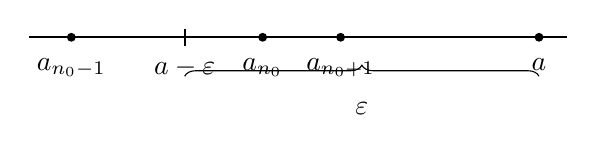
\begin{tikzpicture}[x=0.9cm,y=0.9cm,>=stealth]
  % --- choose positions (kept compact for letter paper) ---
  \def\xLeft{0}
  \def\xAe{2.2}
  \def\xAnz{3.3}
  \def\xAnzp{4.4}
  \def\xA{7.2}

  % number line
  \draw[thick] (\xLeft,0) -- (\xA+0.4,0);

  % tick at a-ε
  \draw[thick] (\xAe,0.12) -- (\xAe,-0.12);

  % points
  \fill (\xLeft+0.6,0) circle (1.6pt) node[below=4pt] {$a_{n_0-1}$};
  \fill (\xAnz,0)      circle (1.6pt) node[below=4pt] {$a_{n_0}$};
  \fill (\xAnzp,0)     circle (1.6pt) node[below=4pt] {$a_{n_0+1}$};
  \fill (\xA,0)        circle (1.6pt) node[below=4pt] {$a$};

  % label a-ε under tick
  \node[below=4pt] at (\xAe,0) {$a-\varepsilon$};

  % epsilon brace from a-ε to a
  \draw[decorate,decoration={brace,amplitude=4pt}]
    (\xAe,-0.55) -- (\xA,-0.55)
    node[midway,below=6pt] {$\varepsilon$};

  % optional: subtle note above (kept short)
  % \node[above=6pt] at ({(\xAe+\xA)/2},0) {$a-\varepsilon < a_n \le a$ for $n\ge n_0$};
\end{tikzpicture}
\end{center}

Thus,
\[
a_n \in N_\varepsilon(a)
\quad \text{for all } n \ge n_0.
\]
This is precisely the definition of convergence. Therefore,
\[
\lim_{n \to \infty} a_n = a.
\]
\end{proof}

% =========================================================
% Real Analysis — Sequences Completion Checklist
% =========================================================


\newpage


\begin{center}
    {\LARGE \textbf{Real Analysis — Sequences Completion Checklist}}\\[1em]
\end{center}

% =========================================================
\section*{I. Real Number Foundations}

\subsection*{Field \& Order Structure}

% ---------------------------------------------------------
% Toolkit
% ---------------------------------------------------------
\begin{tcolorbox}[title=Toolkit: Path]
\begin{tabular}{@{}p{0.28\textwidth}p{0.68\textwidth}@{}}
\textbf{Core items} & Key definitions/results introduced in this file.\\
\textbf{How to use} & Read the boxed items first; proofs and consequences follow.\\
\textbf{Dependencies} & Refer back to earlier sections as needed.\\
\end{tabular}
\end{tcolorbox}


\begin{itemize}
\item \checkbox Field axioms of $\mathbb{R}$
\item \checkbox Order axioms of $\mathbb{R}$
\item \checkbox Trichotomy Law
\item \checkbox Compatibility of order with addition
\item \checkbox Compatibility of order with multiplication
\end{itemize}

\subsection*{Absolute Value}

\begin{itemize}
\item \checkbox Definition of absolute value
\item \checkbox $|x| \ge 0$ and $|x| = 0 \iff x = 0$
\item \checkbox $|xy| = |x||y|$
\item \checkbox Triangle inequality
\item \checkbox Reverse triangle inequality
\end{itemize}

\subsection*{Suprema \& Infima}

\begin{itemize}
\item \checkbox Definition of upper bound
\item \checkbox Definition of lower bound
\item \checkbox Definition of supremum
\item \checkbox Definition of infimum
\item \checkbox Supremum is unique
\item \checkbox Completeness (Least Upper Bound Property)
\end{itemize}

\subsection*{Archimedean Property}

\begin{itemize}
\item \checkbox Archimedean property statement
\item \checkbox Equivalent forms
\item \checkbox Proof that $\frac{1}{n} \to 0$
\end{itemize}

% =========================================================
\section*{II. Basic Sequence Theory}

\subsection*{Definitions}

\begin{itemize}
\item \checkbox Definition of sequence ($\mathbb{N} \to \mathbb{R}$)
\item \checkbox Definition of convergence ($\varepsilon$–$N$ form)
\item \checkbox Negation of convergence
\end{itemize}

\subsection*{Fundamental Theorems}

\begin{itemize}
\item \checkbox Uniqueness of limits
\item \checkbox Convergent $\Rightarrow$ bounded
\end{itemize}

\subsection*{Algebra of Limits}

\begin{itemize}
\item \checkbox Sum rule
\item \checkbox Scalar multiple rule
\item \checkbox Product rule
\item \checkbox Quotient rule (nonzero limit)
\end{itemize}

\subsection*{Order Limit Theorems}

\begin{itemize}
\item \checkbox Limit preserves inequalities
\item \checkbox Squeeze theorem
\end{itemize}

% =========================================================
\section*{III. Structural Sequence Theory}

\subsection*{Monotone Sequences}

\begin{itemize}
\item \checkbox Definition of monotone increasing
\item \checkbox Definition of monotone decreasing
\item \checkbox Monotone Convergence Theorem
\end{itemize}

\subsection*{Subsequences}

\begin{itemize}
\item \checkbox Definition of subsequence
\item \checkbox $n_k$ strictly increasing
\item \checkbox Subsequence of convergent sequence converges to same limit
\item \checkbox Subsequence of subsequence lemma
\item \checkbox Index growth fact: $n_k \ge k$
\end{itemize}

\subsection*{Bolzano--Weierstrass}

\begin{itemize}
\item \checkbox Every bounded sequence has a convergent subsequence
\end{itemize}

% =========================================================
\section*{IV. Cauchy Theory \& Completeness}

\subsection*{Cauchy Sequences}

\begin{itemize}
\item \checkbox Definition of Cauchy sequence
\item \checkbox Convergent $\Rightarrow$ Cauchy
\item \checkbox Cauchy $\Rightarrow$ bounded
\item \checkbox Cauchy $\Rightarrow$ convergent (Completeness of $\mathbb{R}$)
\end{itemize}

% =========================================================
\section*{V. Limit Superior / Limit Inferior}

\begin{itemize}
\item \checkbox Definition of tail set
\item \checkbox Definition of $s_n = \sup_{k \ge n} a_k$
\item \checkbox Definition of $\limsup a_n$
\item \checkbox Definition of $\liminf a_n$
\item \checkbox $\limsup$ always exists (possibly $\pm\infty$)
\item \checkbox $\liminf$ always exists
\item \checkbox $\liminf \le \limsup$
\item \checkbox Convergence $\iff \limsup = \liminf$
\item \checkbox $\limsup$ equals largest subsequential limit
\item \checkbox $\liminf$ equals smallest subsequential limit
\end{itemize}

% =========================================================
\section*{VI. Subsequence Toolkit (Advanced)}

\begin{itemize}
\item \checkbox Finite Partition Convergence Principle
\item \checkbox Residue class convergence
\item \checkbox Even/odd convergence principle
\item \checkbox Dense subsequence criterion
\item \checkbox Diagonal subsequence lemma
\item \checkbox Inherited vs.\ reflected properties
\item \checkbox Tail properties
\item \checkbox Universal subsequence properties
\end{itemize}

% =========================================================
\section*{Final Mastery Check}

\begin{itemize}
\item \checkbox Prove Monotone Convergence from completeness
\item \checkbox Prove Bolzano--Weierstrass
\item \checkbox Prove Cauchy $\iff$ Convergent in $\mathbb{R}$
\item \checkbox Extract convergent subsequences intentionally
\item \checkbox Compute $\limsup$ and $\liminf$ in nontrivial examples
\item \checkbox Characterize convergence via $\limsup/\liminf$
\end{itemize}


\newpage

\clearpage
\section{Worksheets}
% worksheets.tex

% worksheets.tex

% =========================================================
% Worksheet: Abbott — Axiom of Completeness (Bounds / Sup / Inf)
% File: 01-real-analysis/worksheets/abbott.tex
% =========================================================

\subsection{Abbott}

\noindent\textbf{Source.} Stephen Abbott, \textit{Understanding Analysis} (2nd ed.).

\vspace{0.75em}
\begin{center}
\begin{tabular}{|p{5.0cm}|p{9.0cm}|}
\hline
\textbf{Problem ID} & \textbf{Exercise (descriptor)} \\
\hline

% -------------------------
% Chapter 1, §1.3 — The Axiom of Completeness
% -------------------------

\phantomsection
\hypertarget{ws-RA-ABB-C01-S1-3-E02A}{}
\hyperlink{proof-RA-ABB-C01-S1-3-E02A}{\texttt{RA-ABB-C01-S1-3-E02A}}
&
Abbott, Chapter 1, \S1-3, Ex.~1.3.2(a) — Example of $B$ with $\inf B \ge \sup B$ (or impossible).
\\ \hline

\phantomsection
\hypertarget{ws-RA-ABB-C01-S1-3-E02B}{}
\hyperlink{proof-RA-ABB-C01-S1-3-E02B}{\texttt{RA-ABB-C01-S1-3-E02B}}
&
Abbott, Chapter 1, \S1-3, Ex.~1.3.2(b) — Finite set containing $\inf$ but not $\sup$ (or impossible).
\\ \hline

\phantomsection
\hypertarget{ws-RA-ABB-C01-S1-3-E02C}{}
\hyperlink{proof-RA-ABB-C01-S1-3-E02C}{\texttt{RA-ABB-C01-S1-3-E02C}}
&
Abbott, Chapter 1, \S1-3, Ex.~1.3.2(c) — Bounded subset of $\mathbb{Q}$ containing $\sup$ but not $\inf$.
\\ \hline

\phantomsection
\hypertarget{ws-RA-ABB-C01-S1-3-E03A}{}
\hyperlink{proof-RA-ABB-C01-S1-3-E03A}{\texttt{RA-ABB-C01-S1-3-E03A}}
&
Abbott, Chapter 1, \S1-3, Ex.~1.3.3(a) — If $B=\{b\in\mathbb{R}: b\text{ lower bound for }A\}$, show $\sup B=\inf A$.
\\ \hline

\phantomsection
\hypertarget{ws-RA-ABB-C01-S1-3-E03B}{}
\hyperlink{proof-RA-ABB-C01-S1-3-E03B}{\texttt{RA-ABB-C01-S1-3-E03B}}
&
Abbott, Chapter 1, \S1-3, Ex.~1.3.3(b) — Explain why GLB existence need not be an axiom (derive from LUB).
\\ \hline

\phantomsection
\hypertarget{ws-RA-ABB-C01-S1-3-E04}{}
\hyperlink{proof-RA-ABB-C01-S1-3-E04}{\texttt{RA-ABB-C01-S1-3-E04}}
&
Abbott, Chapter 1, \S1-3, Ex.~1.3.4 — Suprema of unions: $\sup(A_1\cup A_2)$, $\sup(\bigcup_{k=1}^n A_k)$, and infinite case.
\\ \hline

\phantomsection
\hypertarget{ws-RA-ABB-C01-S1-3-E05A}{}
\hyperlink{proof-RA-ABB-C01-S1-3-E05A}{\texttt{RA-ABB-C01-S1-3-E05A}}
&
Abbott, Chapter 1, \S1-3, Ex.~1.3.5(a) — If $c\ge 0$, show $\sup(cA)=c\,\sup(A)$ for $cA=\{ca:a\in A\}$.
\\ \hline

\phantomsection
\hypertarget{ws-RA-ABB-C01-S1-3-E05B}{}
\hyperlink{proof-RA-ABB-C01-S1-3-E05B}{\texttt{RA-ABB-C01-S1-3-E05B}}
&
Abbott, Chapter 1, \S1-3, Ex.~1.3.5(b) — Postulate a formula for $\sup(cA)$ when $c<0$.
\\ \hline

\phantomsection
\hypertarget{ws-RA-ABB-C01-S1-3-E06A}{}
\hyperlink{proof-RA-ABB-C01-S1-3-E06A}{\texttt{RA-ABB-C01-S1-3-E06A}}
&
Abbott, Chapter 1, \S1-3, Ex.~1.3.6(a) — For $A+B=\{a+b:a\in A,b\in B\}$, show $s+t$ is an upper bound of $A+B$.
\\ \hline

\phantomsection
\hypertarget{ws-RA-ABB-C01-S1-3-E06B}{}
\hyperlink{proof-RA-ABB-C01-S1-3-E06B}{\texttt{RA-ABB-C01-S1-3-E06B}}
&
Abbott, Chapter 1, \S1-3, Ex.~1.3.6(b) — If $u$ upper bounds $A+B$ and $a\in A$ is fixed, show $t\le u-a$.
\\ \hline

\phantomsection
\hypertarget{ws-RA-ABB-C01-S1-3-E06C}{}
\hyperlink{proof-RA-ABB-C01-S1-3-E06C}{\texttt{RA-ABB-C01-S1-3-E06C}}
&
Abbott, Chapter 1, \S1-3, Ex.~1.3.6(c) — Conclude $\sup(A+B)=s+t$.
\\ \hline

\phantomsection
\hypertarget{ws-RA-ABB-C01-S1-3-E06D}{}
\hyperlink{proof-RA-ABB-C01-S1-3-E06D}{\texttt{RA-ABB-C01-S1-3-E06D}}
&
Abbott, Chapter 1, \S1-3, Ex.~1.3.6(d) — Re-prove $\sup(A+B)=\sup A+\sup B$ using Lemma~1.3.8.
\\ \hline

\phantomsection
\hypertarget{ws-RA-ABB-C01-S1-3-E07}{}
\hyperlink{proof-RA-ABB-C01-S1-3-E07}{\texttt{RA-ABB-C01-S1-3-E07}}
&
Abbott, Chapter 1, \S1-3, Ex.~1.3.7 — If $a$ is an upper bound for $A$ and $a\in A$, prove $a=\sup A$.
\\ \hline

\phantomsection
\hypertarget{ws-RA-ABB-C01-S1-3-E08A}{}
\hyperlink{proof-RA-ABB-C01-S1-3-E08A}{\texttt{RA-ABB-C01-S1-3-E08A}}
&
Abbott, Chapter 1, \S1-3, Ex.~1.3.8(a) — Compute $\sup/\inf$ of $\{m/n:m,n\in\mathbb{N},\ m<n\}$.
\\ \hline

\phantomsection
\hypertarget{ws-RA-ABB-C01-S1-3-E08B}{}
\hyperlink{proof-RA-ABB-C01-S1-3-E08B}{\texttt{RA-ABB-C01-S1-3-E08B}}
&
Abbott, Chapter 1, \S1-3, Ex.~1.3.8(b) — Compute $\sup/\inf$ of $\{(-1)^m/n:m,n\in\mathbb{N}\}$.
\\ \hline

\phantomsection
\hypertarget{ws-RA-ABB-C01-S1-3-E08C}{}
\hyperlink{proof-RA-ABB-C01-S1-3-E08C}{\texttt{RA-ABB-C01-S1-3-E08C}}
&
Abbott, Chapter 1, \S1-3, Ex.~1.3.8(c) — Compute $\sup/\inf$ of $\{n/(3n+1):n\in\mathbb{N}\}$.
\\ \hline

\phantomsection
\hypertarget{ws-RA-ABB-C01-S1-3-E08D}{}
\hyperlink{proof-RA-ABB-C01-S1-3-E08D}{\texttt{RA-ABB-C01-S1-3-E08D}}
&
Abbott, Chapter 1, \S1-3, Ex.~1.3.8(d) — Compute $\sup/\inf$ of $\{m/(m+n):m,n\in\mathbb{N}\}$.
\\ \hline

\phantomsection
\hypertarget{ws-RA-ABB-C01-S1-3-E09A}{}
\hyperlink{proof-RA-ABB-C01-S1-3-E09A}{\texttt{RA-ABB-C01-S1-3-E09A}}
&
Abbott, Chapter 1, \S1-3, Ex.~1.3.9(a) — If $\sup A<\sup B$, show $\exists b\in B$ that is an upper bound for $A$.
\\ \hline

\phantomsection
\hypertarget{ws-RA-ABB-C01-S1-3-E09B}{}
\hyperlink{proof-RA-ABB-C01-S1-3-E09B}{\texttt{RA-ABB-C01-S1-3-E09B}}
&
Abbott, Chapter 1, \S1-3, Ex.~1.3.9(b) — Counterexample if only $\sup A\le \sup B$ is assumed.
\\ \hline

\phantomsection
\hypertarget{ws-RA-ABB-C01-S1-3-E10A}{}
\hyperlink{proof-RA-ABB-C01-S1-3-E10A}{\texttt{RA-ABB-C01-S1-3-E10A}}
&
Abbott, Chapter 1, \S1-3, Ex.~1.3.10(a) — Use completeness to prove the Cut Property.
\\ \hline

\end{tabular}
\end{center}


% =========================================================
% Worksheet: Ross — Bounds / Sup / Inf / Density (Chapter 4)
% File: 05-real-line-foundations/worksheets/ross.tex
% =========================================================

\subsection{Ross}

\noindent\textbf{Source.} Kenneth A. Ross, \textit{Elementary Analysis: The Theory of Calculus} (2nd ed.).

\vspace{0.75em}
\begin{center}
\begin{tabular}{|p{5.0cm}|p{9.0cm}|}
\hline
\textbf{Problem ID} & \textbf{Exercise (descriptor)} \\
\hline

% -------------------------
% Chapter 4 — Suprema, Infima, and Density
% -------------------------

\phantomsection
\hypertarget{ws-RA-ROS-C04-E045}{}
\hyperlink{proof-RA-ROS-C04-E045}{\texttt{RA-ROS-C04-E045}}
&
Ross, Chapter 4, Ex.~4.5 — If $\sup S\in S$, prove $\sup S=\max S$ (for nonempty $S\subseteq\mathbb{R}$ bounded above).
\\ \hline

\phantomsection
\hypertarget{ws-RA-ROS-C04-E046A}{}
\hyperlink{proof-RA-ROS-C04-E046A}{\texttt{RA-ROS-C04-E046A}}
&
Ross, Chapter 4, Ex.~4.6(a) — For nonempty bounded $S\subseteq\mathbb{R}$, prove $\inf S \le \sup S$.
\\ \hline

\phantomsection
\hypertarget{ws-RA-ROS-C04-E046B}{}
\hyperlink{proof-RA-ROS-C04-E046B}{\texttt{RA-ROS-C04-E046B}}
&
Ross, Chapter 4, Ex.~4.6(b) — Describe $S$ if $\inf S=\sup S$.
\\ \hline

\phantomsection
\hypertarget{ws-RA-ROS-C04-E047A}{}
\hyperlink{proof-RA-ROS-C04-E047A}{\texttt{RA-ROS-C04-E047A}}
&
Ross, Chapter 4, Ex.~4.7(a) — If $S\subseteq T$, prove $\inf T \le \inf S \le \sup S \le \sup T$.
\\ \hline

\phantomsection
\hypertarget{ws-RA-ROS-C04-E047B}{}
\hyperlink{proof-RA-ROS-C04-E047B}{\texttt{RA-ROS-C04-E047B}}
&
Ross, Chapter 4, Ex.~4.7(b) — Prove $\sup(S\cup T)=\max\{\sup S,\sup T\}$ (do not assume $S\subseteq T$).
\\ \hline

\phantomsection
\hypertarget{ws-RA-ROS-C04-E048A}{}
\hyperlink{proof-RA-ROS-C04-E048A}{\texttt{RA-ROS-C04-E048A}}
&
Ross, Chapter 4, Ex.~4.8(a) — If $s\le t$ for all $s\in S$, $t\in T$, observe $S$ bounded above and $T$ bounded below.
\\ \hline

\phantomsection
\hypertarget{ws-RA-ROS-C04-E048B}{}
\hyperlink{proof-RA-ROS-C04-E048B}{\texttt{RA-ROS-C04-E048B}}
&
Ross, Chapter 4, Ex.~4.8(b) — Under Ex.~4.8 hypotheses, prove $\sup S \le \inf T$.
\\ \hline

\phantomsection
\hypertarget{ws-RA-ROS-C04-E048C}{}
\hyperlink{proof-RA-ROS-C04-E048C}{\texttt{RA-ROS-C04-E048C}}
&
Ross, Chapter 4, Ex.~4.8(c) — Give an example with $S\cap T\neq\varnothing$.
\\ \hline

\phantomsection
\hypertarget{ws-RA-ROS-C04-E048D}{}
\hyperlink{proof-RA-ROS-C04-E048D}{\texttt{RA-ROS-C04-E048D}}
&
Ross, Chapter 4, Ex.~4.8(d) — Give an example with $\sup S=\inf T$ and $S\cap T=\varnothing$.
\\ \hline

\phantomsection
\hypertarget{ws-RA-ROS-C04-E049}{}
\hyperlink{proof-RA-ROS-C04-E049}{\texttt{RA-ROS-C04-E049}}
&
Ross, Chapter 4, Ex.~4.9 — Complete the proof that $\inf S=-\sup(-S)$ (Cor.~4.5), by proving (1) and (2).
\\ \hline

\phantomsection
\hypertarget{ws-RA-ROS-C04-E0410}{}
\hyperlink{proof-RA-ROS-C04-E0410}{\texttt{RA-ROS-C04-E0410}}
&
Ross, Chapter 4, Ex.~4.10 — If $a>0$, show $\exists n\in\mathbb{N}$ with $\frac1n<a<n$.
\\ \hline

\phantomsection
\hypertarget{ws-RA-ROS-C04-E0411}{}
\hyperlink{proof-RA-ROS-C04-E0411}{\texttt{RA-ROS-C04-E0411}}
&
Ross, Chapter 4, Ex.~4.11 — If $a<b$, use density of $\mathbb{Q}$ to show infinitely many rationals lie between $a$ and $b$.
\\ \hline

\phantomsection
\hypertarget{ws-RA-ROS-C04-E0412}{}
\hyperlink{proof-RA-ROS-C04-E0412}{\texttt{RA-ROS-C04-E0412}}
&
Ross, Chapter 4, Ex.~4.12 — If $a<b$, prove $\exists x\in\mathbb{I}$ with $a<x<b$ (irrationals; hint uses $\{r+\sqrt2:r\in\mathbb{Q}\}$).
\\ \hline

\end{tabular}
\end{center}


% =========================================================
% Worksheet: Johar — Sequences and Limits
% File: real-line-foundations/worksheets/johar.tex
% =========================================================

\subsection{Johar}

\noindent\textbf{Source.} Syafiq Johar, \textit{The Big Book of Real Analysis}.

\vspace{0.75em}
\begin{center}
\begin{tabular}{|p{5.0cm}|p{9.0cm}|}
\hline
\textbf{Problem ID} & \textbf{Exercise (descriptor)} \\
\hline

% -------------------------------------------------
% Chapter 5 — Exercise 5-1
% -------------------------------------------------

\phantomsection
\hypertarget{ws-RA-JOH-C05-S5-1-E01A}{}
\hyperlink{proof-RA-JOH-C05-S5-1-E01A}{\texttt{RA-JOH-C05-S5-1-E01A}}
&
Ex.~5.1(a) — Show $a_n\to 0$ for $a_n=\dfrac{1}{n^2+3}$.
\\ \hline

\phantomsection
\hypertarget{ws-RA-JOH-C05-S5-1-E01B}{}
\hyperlink{proof-RA-JOH-C05-S5-1-E01B}{\texttt{RA-JOH-C05-S5-1-E01B}}
&
Ex.~5.1(b) — Show $a_n\to 0$ for $a_n=\dfrac{1}{n-\frac{5}{2}}$.
\\ \hline

\phantomsection
\hypertarget{ws-RA-JOH-C05-S5-1-E01C}{}
\hyperlink{proof-RA-JOH-C05-S5-1-E01C}{\texttt{RA-JOH-C05-S5-1-E01C}}
&
Ex.~5.1(c) — Show $a_n\to 0$ for $a_n=\dfrac{1}{n\left(n-\frac{1}{2}\right)}$.
\\ \hline

\phantomsection
\hypertarget{ws-RA-JOH-C05-S5-1-E01D}{}
\hyperlink{proof-RA-JOH-C05-S5-1-E01D}{\texttt{RA-JOH-C05-S5-1-E01D}}
&
Ex.~5.1(d) — Show $a_n\to 0$ for $a_n=\dfrac{1}{\sqrt{5n}-1}$.
\\ \hline

\phantomsection
\hypertarget{ws-RA-JOH-C05-S5-1-E01E}{}
\hyperlink{proof-RA-JOH-C05-S5-1-E01E}{\texttt{RA-JOH-C05-S5-1-E01E}}
&
Ex.~5.1(e) — Show $a_n\to 0$ for $a_n=\dfrac{\sin(n)}{n}$.
\\ \hline

\phantomsection
\hypertarget{ws-RA-JOH-C05-S5-1-E01F}{}
\hyperlink{proof-RA-JOH-C05-S5-1-E01F}{\texttt{RA-JOH-C05-S5-1-E01F}}
&
Ex.~5.1(f) — Prime/non-prime definition.
\\ \hline

\phantomsection
\hypertarget{ws-RA-JOH-C05-S5-1-E01G}{}
\hyperlink{proof-RA-JOH-C05-S5-1-E01G}{\texttt{RA-JOH-C05-S5-1-E01G}}
&
Ex.~5.1(g) — $a_n=\sqrt{n+1}-\sqrt{n}$.
\\ \hline

\phantomsection
\hypertarget{ws-RA-JOH-C05-S5-1-E01H}{}
\hyperlink{proof-RA-JOH-C05-S5-1-E01H}{\texttt{RA-JOH-C05-S5-1-E01H}}
&
Ex.~5.1(h) — $a_n=n-\sqrt{n^2+\sqrt{n}}$.
\\ \hline


% -------------------------------------------------
% Additional Chapter 5 Exercises
% -------------------------------------------------

\phantomsection
\hypertarget{ws-RA-JOH-C05-S5-7}{}
\hyperlink{proof-RA-JOH-C05-S5-7}{\texttt{RA-JOH-C05-S5-7}}
&
Ex.~5.7 — Convergence from even/odd and modular subsequences.
\\ \hline

\phantomsection
\hypertarget{ws-RA-JOH-C05-S5-8}{}
\hyperlink{proof-RA-JOH-C05-S5-8}{\texttt{RA-JOH-C05-S5-8}}
&
Ex.~5.8 — $|a_n-b_n|\to 0$ and counterexample.
\\ \hline

\phantomsection
\hypertarget{ws-RA-JOH-C05-S5-17}{}
\hyperlink{proof-RA-JOH-C05-S5-17}{\texttt{RA-JOH-C05-S5-17}}
&
Ex.~5.17 — Limits of $r^{1/n}$ and related sequences.
\\ \hline

\phantomsection
\hypertarget{ws-RA-JOH-C05-S5-18}{}
\hyperlink{proof-RA-JOH-C05-S5-18}{\texttt{RA-JOH-C05-S5-18}}
&
Ex.~5.18 — Applications of $n^{1/n}\to 1$.
\\ \hline

\phantomsection
\hypertarget{ws-RA-JOH-C05-S5-34}{}
\hyperlink{proof-RA-JOH-C05-S5-34}{\texttt{RA-JOH-C05-S5-34}}
&
Ex.~5.34 — limsup and liminf algebra rules.
\\ \hline

\end{tabular}
\end{center}



\section{Proofs}
% -------------------------
% Abbott — Chapter 1, §1.3 (Axiom of Completeness)
% -------------------------
\newpage

% =========================================================
% Proof Planning Worksheet (Quantifier-Aware Version)
% Theorem: A convergent sequence has a unique limit
% =========================================================

\section*{Proof Planning Worksheet}

\textbf{Theorem (as written).}  
A convergent sequence has a unique limit.

\bigskip

% ---------------------------------------------------------
\subsection*{1. Quantifier Detection (Natural Language Analysis)}

Rewrite the statement in explicit English,
making all hidden quantifiers visible.

\begin{itemize}
    \item Is the phrase generic or existential?
    \item What quantifier does it encode?
    \item Is the statement conditional?
    \item Is the statement conjunctive/disjunctive or compound?
\end{itemize}

Write the expanded English sentence below: \\
 \\
For every sequence, if the sequence converges, then there exists a real number L such that the sequence converges to L,
and if the sequence also converges to some real number M, then M=L.
\vspace{3cm}
\hrule
\vspace{1cm}

% ---------------------------------------------------------
\subsection*{2. Logical Skeleton (Propositional Form)}

Abstract the theorem into propositional structure.

Let:

\[
C(x) := \text{“$x$ is a convergent sequence”}
\]
\[
C(x) := \exists \ell \; L(x,\ell).
\]

\[
Q(x) := \text{“$x$ has at most one limit.”}
\]
\[
Q(x) :=
\forall \ell_1 \forall \ell_2
\bigl(
L(x,\ell_1) \land L(x,\ell_2)
\rightarrow
\ell_1 = \ell_2
\bigr).
\]
Rewrite the theorem schematically:

\vspace{2cm}
\hrule
\vspace{1cm}

% ---------------------------------------------------------
\subsection*{3. Predicate-Level Formalization}

Now rewrite the theorem with explicit quantifiers:

\vspace{3cm}
\hrule
\vspace{1cm}

% ---------------------------------------------------------
\subsection*{4. Expand the Meaning of “Unique”}

Write the full logical expansion of:

\[
\exists! L \text{ such that } P(L)
\]

\vspace{3cm}
\hrule
\vspace{1cm}

% ---------------------------------------------------------
\subsection*{5. Separate Existence from Uniqueness}

Is existence already contained in the hypothesis?
Or must it be proved?

Explain clearly which part of uniqueness remains to be shown:

\vspace{3cm}
\hrule
\vspace{1cm}

% ---------------------------------------------------------
\subsection*{6. Structural Decomposition of the Proof}

Before writing any proof, answer:

\begin{itemize}
    \item What object is fixed?
    \item What hypothesis is assumed?
    \item What must ultimately be shown?
    \item What equality (if any) must be derived?
\end{itemize}

Write these in clean logical phrases (not narrative prose):

\vspace{4cm}
\hrule
\vspace{1cm}

% ---------------------------------------------------------
\subsection*{7. Quantifier Expansion of Definitions}

Write the full quantified definition of:

\begin{itemize}
    \item Convergence
    \item Limit
\end{itemize}

Be explicit about:

\[
\forall \varepsilon \;
\exists N \;
\forall n \ge N
\]

\vspace{5cm}
\hrule
\vspace{1cm}

% ---------------------------------------------------------
\subsection*{8. Scope and Dependency Tracking}

For each quantifier appearing in the theorem or definitions:

\begin{itemize}
    \item Identify what it ranges over.
    \item Identify what it may depend on.
    \item Identify which step of the proof will eliminate it.
\end{itemize}

\vspace{4cm}
\hrule

\newpage
\begin{theorem}
A convergent sequence has a unique limit.
\end{theorem}

\begin{proof}
\noindent
\begin{minipage}[t]{0.48\textwidth}
\textbf{Symmetric Form}

\medskip

Let $(x_n)$ be a convergent sequence.

Assume $x_n \to \ell_1$ and $x_n \to \ell_2$.

Let $\varepsilon > 0$ be arbitrary.

From $x_n \to \ell_1$, there exists $N_1$ such that
\[
n \ge N_1 \Rightarrow |x_n - \ell_1| < \varepsilon/2.
\]

From $x_n \to \ell_2$, there exists $N_2$ such that
\[
n \ge N_2 \Rightarrow |x_n - \ell_2| < \varepsilon/2.
\]

Let $N = \max\{N_1, N_2\}$.

Then for $n \ge N$,
\[
|\ell_1 - \ell_2|
\le |\ell_1 - x_n| + |x_n - \ell_2|
< \varepsilon/2 + \varepsilon/2
= \varepsilon.
\]

Since $\varepsilon > 0$ was arbitrary,
$|\ell_1 - \ell_2| = 0$, hence
\[
\ell_1 = \ell_2.
\]

\medskip

Thus the limit is unique.
\end{minipage}
\hfill
\begin{minipage}[t]{0.48\textwidth}
\textbf{Witness-Based Form}

\medskip

Let $(x_n)$ be a convergent sequence.

Then there exists $L_c$ such that
\[
x_n \to L_c.
\]

Let $m$ be any real number and assume
\[
x_n \to m.
\]

Let $\varepsilon > 0$ be arbitrary.

From $x_n \to L_c$, there exists $N_1$ such that
\[
n \ge N_1 \Rightarrow |x_n - L_c| < \varepsilon/2.
\]

From $x_n \to m$, there exists $N_2$ such that
\[
n \ge N_2 \Rightarrow |x_n - m| < \varepsilon/2.
\]

Let $N = \max\{N_1, N_2\}$.

Then for $n \ge N$,
\[
|m - L_c|
\le |m - x_n| + |x_n - L_c|
< \varepsilon/2 + \varepsilon/2
= \varepsilon.
\]

Since $\varepsilon > 0$ was arbitrary,
$|m - L_c| = 0$, hence
\[
m = L_c.
\]

\medskip

Thus every limit equals $L_c$, so the limit is unique.
\end{minipage}
\end{proof}
\newpage

\begin{theorem}[Every Cauchy sequence in $\mathbb{R}$ is bounded]
If $(s_n)$ is a Cauchy sequence in $\mathbb{R}$, then $(s_n)$ is bounded.
\end{theorem}

\begin{proof}
Assume $(s_n)$ is a Cauchy sequence.  Then
\[
\forall \varepsilon > 0\;\exists N\in\mathbb{N}\;\forall m,n\ge N:\ |s_m-s_n|<\varepsilon.
\]
Choose $\varepsilon = 1$.  Then there exists $N_0\in\mathbb{N}$ such that
\[
\forall m,n\ge N_0:\ |s_m-s_n|<1.
\]
In particular, fixing $n=N_0$ and letting $m\ge N_0$ vary, we obtain
\[
\forall m\ge N_0:\ |s_m-s_{N_0}|<1.
\]
For every $m\ge N_0$, the triangle inequality gives
\[
|s_m|
= |(s_m-s_{N_0})+s_{N_0}|
\le |s_m-s_{N_0}|+|s_{N_0}|
< 1+|s_{N_0}|.
\]
Define the tail bound
\[
M_{\mathrm{tail}} := 1+|s_{N_0}|.
\]
Then
\[
\forall n\ge N_0:\ |s_n|\le M_{\mathrm{tail}}.
\]

Now consider the finite set of the first $N_0-1$ terms
\[
\{|s_1|,|s_2|,\dots,|s_{N_0-1}|\}.
\]
If $N_0=1$, this set is empty; otherwise it is finite and therefore has a maximum.
Define
\[
M_{\mathrm{head}} :=
\begin{cases}
0, & N_0=1,\\[4pt]
\max\{|s_1|,|s_2|,\dots,|s_{N_0-1}|\}, & N_0\ge 2.
\end{cases}
\]
Then
\[
\forall n< N_0:\ |s_n|\le M_{\mathrm{head}}.
\]

Finally, define
\[
M := \max\{M_{\mathrm{head}},\,M_{\mathrm{tail}}\}.
\]
We claim that $|s_n|\le M$ for all $n\in\mathbb{N}$.
Indeed, if $n<N_0$ then $|s_n|\le M_{\mathrm{head}}\le M$, and if $n\ge N_0$ then
$|s_n|\le M_{\mathrm{tail}}\le M$.  Hence
\[
\forall n\in\mathbb{N}:\ |s_n|\le M.
\]
Therefore $(s_n)$ is bounded.
\end{proof}

\newpage

% =========================================================
% Proof Planning Worksheet (Quantifier-Aware Version)
% Theorem: If a sequence converges, then every subsequence converges
%         to the same limit.
% =========================================================


\begin{center}
\begin{tabular}{|p{0.62\linewidth}|p{0.33\linewidth}|}
\hline
\textbf{Statement} & \textbf{Justification} \\
\hline

1.\;\; Let $a$ be arbitrary. &
$\forall$-Intro setup (arbitrary object) \\

2.\;\; Assume $\mathrm{Convergent}(a)$. &
Assumption for $\to$-Intro \\

3.\;\; $\exists L\in\mathbb R\;\forall \varepsilon>0\;\exists N\in\mathbb N\;\forall n\in\mathbb N\;
(n\ge N \to |a(n)-L|<\varepsilon)$. &
Unfold definition of $\mathrm{Convergent}(a)$ \\

4.\;\; Let $L\in\mathbb R$ such that
$\forall \varepsilon>0\;\exists N\in\mathbb N\;\forall n\in\mathbb N\;
(n\ge N \to |a(n)-L|<\varepsilon)$. &
$\exists$-Elim on (3) (introduce witness $L$) \\

5.\;\; Take $\varepsilon := 1$. &
Instantiation (choose a specific positive $\varepsilon$) \\

6.\;\; $1>0$. &
Arithmetic fact \\

7.\;\; $\exists N\in\mathbb N\;\forall n\in\mathbb N\;(n\ge N\to |a(n)-L|<1)$. &
From (4),(5),(6) by $\forall$-Elim then $\to$-Elim \\

8.\;\; Let $N\in\mathbb N$ such that
$\forall n\in\mathbb N\;(n\ge N\to |a(n)-L|<1)$. &
$\exists$-Elim on (7) (introduce witness $N$) \\

9.\;\; $\forall n\in\mathbb N\;(n\ge N\to |a(n)|\le |L|+1)$. &
From (8) using lemma:
$|x-L|<1\to |x|\le |L|+1$ (instantiate $x:=a(n)$) \\

10.\;\; Define $B_0 := \max\{|a(1)|,\dots,|a(N)|\}$. &
Definition / existence of finite max \\

11.\;\; $\forall k\in\mathbb N\;(k\le N\to |a(k)|\le B_0)$. &
Property of $\max$ / finite bound axiom \\

12.\;\; Let $M := \max\{B_0,\ |L|+1\}$. &
Definition of a real number $M$ \\

13.\;\; $\forall n\in\mathbb N\;(n\le N\to |a(n)|\le M)$. &
From (11),(12) and $\max$-monotonicity \\

14.\;\; $\forall n\in\mathbb N\;(n\ge N\to |a(n)|\le M)$. &
From (9),(12) and $\max$-monotonicity \\

15.\;\; $\forall n\in\mathbb N\;(|a(n)|\le M)$. &
From (13),(14) and trichotomy: $(n\le N)\lor(n\ge N)$,
then cases + $\lor$-Elim \\

16.\;\; $\exists M\in\mathbb R\;\forall n\in\mathbb N\;(|a(n)|\le M)$. &
$\exists$-Intro using witness $M$ from (12),(15) \\

17.\;\; $\mathrm{Bounded}(a)$. &
Fold definition of $\mathrm{Bounded}(a)$ \\

18.\;\; $\mathrm{Convergent}(a)\to \mathrm{Bounded}(a)$. &
$\to$-Intro discharging assumption (2) \\

19.\;\; $\forall a\;(\mathrm{Convergent}(a)\to \mathrm{Bounded}(a))$. &
$\forall$-Intro from (1),(18) \\

\hline
\end{tabular}
\end{center}


\newpage


% -------------------------
% Abbott — Chapter 1, §1.3 (Axiom of Completeness)
% -------------------------
\input{real-line-foundations/proofs/abbott/RA-ABB-C01-S1-3-E02A}
% --------------------------------------
% Proof: RA-ABB-C01-S1-3-E02B
% --------------------------------------
\clearpage
\phantomsection
\hypertarget{proof-RA-ABB-C01-S1-3-E02B}{}

\section*{Proof — RA-ABB-C01-S1-3-E02B}

\noindent
\hyperlink{ws-RA-ABB-C01-S1-3-E02B}{\textbf{← Back to worksheet}}

\noindent
\textbf{Source.}
\srccite{AbbottUnderstandingAnalysis}{Chapter~1, \S1-3, Exercise~1.3.2(b)}.

\vspace{0.75em}

\noindent
\textbf{Goal.} Give an example of a finite set that contains its infimum but not its supremum, or state that the request is impossible.

\vspace{0.75em}

\noindent
\textbf{Proof (stub).}
\begin{itemize}
\item Recall: finite nonempty subsets of $\mathbb{R}$ attain both a minimum and a maximum.
\item Translate “contains its infimum” as “has a least element,” and “contains its supremum” as “has a greatest element.”
\item Either (i) prove impossibility, or (ii) if you think it’s possible, produce a counterexample and verify carefully.
\end{itemize}

\vspace{1em}
\noindent
\hyperlink{ws-RA-ABB-C01-S1-3-E02B}{\textbf{← Back to worksheet}}
% --------------------------------------
% Proof: RA-ABB-C01-S1-3-E02C
% --------------------------------------
\clearpage
\phantomsection
\hypertarget{proof-RA-ABB-C01-S1-3-E02C}{}

\section*{Proof — RA-ABB-C01-S1-3-E02C}

\noindent
\hyperlink{ws-RA-ABB-C01-S1-3-E02C}{\textbf{← Back to worksheet}}

\noindent
\textbf{Source.}
\srccite{AbbottUnderstandingAnalysis}{Chapter~1, \S1-3, Exercise~1.3.2(c)}.

\vspace{0.75em}

\noindent
\textbf{Goal.} Give an example of a bounded subset of $\mathbb{Q}$ that contains its supremum but not its infimum.

\vspace{0.75em}

\noindent
\textbf{Proof (stub).}
\begin{itemize}
\item Choose a subset $A \subseteq \mathbb{Q}$ that is bounded.
\item Ensure $\sup A \in A$ (so the supremum is attained).
\item Ensure $\inf A \notin A$ (so the infimum is not attained).
\item Verify: (i) boundedness, (ii) candidate is an upper bound and least, (iii) candidate is a lower bound and greatest, and (iv) membership/non-membership claims.
\end{itemize}

\vspace{1em}
\noindent
\hyperlink{ws-RA-ABB-C01-S1-3-E02C}{\textbf{← Back to worksheet}}


\input{real-line-foundations/proofs/abbott/RA-ABB-C01-S1-3-E03A}
\input{real-line-foundations/proofs/abbott/RA-ABB-C01-S1-3-E03B}

% --------------------------------------
% Proof: RA-ABB-C01-S1-3-E04
% --------------------------------------
\clearpage
\phantomsection
\hypertarget{proof-RA-ABB-C01-S1-3-E04}{}

\section*{Proof — RA-ABB-C01-S1-3-E04}

\noindent
\hyperlink{ws-RA-ABB-C01-S1-3-E04}{\textbf{← Back to worksheet}}

\noindent
\textbf{Source.}
\srccite{AbbottUnderstandingAnalysis}{Chapter~1, \S1-3, Exercise~1.3.4}.

\vspace{0.75em}

\noindent
\textbf{Goal.}
Let $A_1,A_2,A_3,\dots$ be a collection of nonempty sets, each of which is bounded above.
\begin{enumerate}[label=(\alph*)]
\item Find a formula for $\sup(A_1\cup A_2)$, and extend to $\sup\!\Big(\bigcup_{k=1}^n A_k\Big)$.
\item Consider $\sup\!\Big(\bigcup_{k=1}^\infty A_k\Big)$. Does the formula in (a) extend to the infinite case?
\end{enumerate}

\vspace{0.75em}

\noindent
\textbf{Proof.}



\begin{enumerate}[label=(\alph*)]

\item
Let $A_1,A_2 \subseteq \mathbb{R}$ be nonempty and bounded above.
Define
\[
s_1 := \sup A_1, \qquad s_2 := \sup A_2,
\]
and set
\[
m := \max\{s_1,s_2\}.
\]

We show that $m = \sup(A_1 \cup A_2)$.

First, we verify that $m$ is an upper bound of $A_1 \cup A_2$.
Let $x \in A_1 \cup A_2$. Then either $x \in A_1$ or $x \in A_2$.
If $x \in A_1$, then $x \le s_1 \le m$.
If $x \in A_2$, then $x \le s_2 \le m$.
Hence $x \le m$ in all cases, and $m$ is an upper bound of $A_1 \cup A_2$.

Next, let $u$ be any upper bound of $A_1 \cup A_2$.
Because $A_1 \subseteq A_1 \cup A_2$ and $A_2 \subseteq A_1 \cup A_2$,
the number $u$ is an upper bound of both $A_1$ and $A_2$.
Therefore,
\[
s_1 \le u \quad \text{and} \quad s_2 \le u,
\]
which implies $m = \max\{s_1,s_2\} \le u$.

Thus $m$ is the least upper bound of $A_1 \cup A_2$, and
\[
\sup(A_1 \cup A_2) = \max\{\sup A_1,\sup A_2\}.
\]

The same argument extends to finitely many sets.
If $A_1,\dots,A_n$ are nonempty and bounded above, then
\[
\sup\!\Big(\bigcup_{k=1}^n A_k\Big)
= \max\{\sup A_1,\dots,\sup A_n\}.
\]

\item
We now consider the infinite union $\bigcup_{k=1}^\infty A_k$.

In general, the formula in part (a) does \emph{not} extend to the infinite case.
The set $\{\sup A_k : k \in \mathbb{N}\}$ need not have a maximum, and the union
$\bigcup_{k=1}^\infty A_k$ may fail to be bounded above.

However, if $\bigcup_{k=1}^\infty A_k$ \emph{is} bounded above, then the correct
relationship is
\[
\sup\!\Big(\bigcup_{k=1}^\infty A_k\Big)
= \sup_{k \in \mathbb{N}} (\sup A_k).
\]

To justify this, let $s_k := \sup A_k$ and define
\[
S := \sup_{k \in \mathbb{N}} s_k.
\]

First, we show that $S$ is an upper bound of $\bigcup_{k=1}^\infty A_k$.
If $x \in \bigcup_{k=1}^\infty A_k$, then $x \in A_j$ for some $j$.
Thus $x \le s_j \le S$, so $x \le S$.

Next, let $u$ be any upper bound of $\bigcup_{k=1}^\infty A_k$.
Then $u$ is an upper bound of each $A_k$, so $s_k \le u$ for all $k$.
Hence $u$ is an upper bound of the set $\{s_k\}$, which implies $S \le u$.

Therefore, $S$ is the least upper bound of $\bigcup_{k=1}^\infty A_k$, and
\[
\sup\!\Big(\bigcup_{k=1}^\infty A_k\Big)
= \sup_{k \in \mathbb{N}} (\sup A_k).
\]

\end{enumerate}



\vspace{1em}
\noindent
\hyperlink{ws-RA-ABB-C01-S1-3-E04}{\textbf{← Back to worksheet}}



\input{real-line-foundations/proofs/abbott/RA-ABB-C01-S1-3-E05A}
% --------------------------------------
% Proof: RA-ABB-C01-S1-3-E05B
% --------------------------------------
\clearpage
\phantomsection
\hypertarget{proof-RA-ABB-C01-S1-3-E05B}{}

\section*{Proof — RA-ABB-C01-S1-3-E05B}

\noindent
\hyperlink{ws-RA-ABB-C01-S1-3-E05B}{\textbf{← Back to worksheet}}

\noindent
\textbf{Source.}
\srccite{AbbottUnderstandingAnalysis}{Chapter~1, \S1-3, Exercise~1.3.5(b)}.

\vspace{0.75em}

\noindent
\textbf{Goal.} Postulate a similar type of statement for $\sup(cA)$ for the case $c<0$.

\vspace{0.75em}

\noindent
\textbf{Proof (stub).}


\vspace{1em}
\noindent
\hyperlink{ws-RA-ABB-C01-S1-3-E05B}{\textbf{← Back to worksheet}}



\input{real-line-foundations/proofs/abbott/RA-ABB-C01-S1-3-E06A}
\input{real-line-foundations/proofs/abbott/RA-ABB-C01-S1-3-E06B}
\input{real-line-foundations/proofs/abbott/RA-ABB-C01-S1-3-E06C}
\input{real-line-foundations/proofs/abbott/RA-ABB-C01-S1-3-E06D}

% --------------------------------------
% Proof: RA-ABB-C01-S1-3-E07
% --------------------------------------
\clearpage
\phantomsection
\hypertarget{proof-RA-ABB-C01-S1-3-E07}{}

\section*{Proof — RA-ABB-C01-S1-3-E07}

\noindent
\hyperlink{ws-RA-ABB-C01-S1-3-E07}{\textbf{← Back to worksheet}}

\noindent
\textbf{Source.}
\srccite{AbbottUnderstandingAnalysis}{Chapter~1, \S1-3, Exercise~1.3.7}.

\vspace{0.75em}

\noindent
\textbf{Goal.} Prove that if $a$ is an upper bound for $A$, and if $a\in A$, then $a=\sup A$.

\vspace{0.75em}

\noindent
\textbf{Proof (stub).}

\vspace{1em}
\noindent
\hyperlink{ws-RA-ABB-C01-S1-3-E07}{\textbf{← Back to worksheet}}


% --------------------------------------
% Proof: RA-ABB-C01-S1-3-E08A
% --------------------------------------
\clearpage
\phantomsection
\hypertarget{proof-RA-ABB-C01-S1-3-E08A}{}

\section*{Proof — RA-ABB-C01-S1-3-E08A}

\noindent
\hyperlink{ws-RA-ABB-C01-S1-3-E08A}{\textbf{← Back to worksheet}}

\noindent
\textbf{Source.}
\srccite{AbbottUnderstandingAnalysis}{Chapter~1, \S1-3, Exercise~1.3.8(a)}.

\vspace{0.75em}

\noindent
\textbf{Goal.} Compute (no proofs) $\sup$ and $\inf$ (if they exist) of
\[
\left\{\frac{m}{n}: m,n\in\mathbb{N}\ \text{with } m<n\right\}.
\]

\vspace{0.75em}

\noindent
\textbf{Work (stub).}

\vspace{1em}
\noindent
\hyperlink{ws-RA-ABB-C01-S1-3-E08A}{\textbf{← Back to worksheet}}

\input{real-line-foundations/proofs/abbott/RA-ABB-C01-S1-3-E08B}
% --------------------------------------
% Proof: RA-ABB-C01-S1-3-E08C
% --------------------------------------
\clearpage
\phantomsection
\hypertarget{proof-RA-ABB-C01-S1-3-E08C}{}

\section*{Proof — RA-ABB-C01-S1-3-E08C}

\noindent
\hyperlink{ws-RA-ABB-C01-S1-3-E08C}{\textbf{← Back to worksheet}}

\noindent
\textbf{Source.}
\srccite{AbbottUnderstandingAnalysis}{Chapter~1, \S1-3, Exercise~1.3.8(c)}.

\vspace{0.75em}

\noindent
\textbf{Goal.} Compute (no proofs) $\sup$ and $\inf$ (if they exist) of
\[
\left\{\frac{n}{3n+1}: n\in\mathbb{N}\right\}.
\]

\vspace{0.75em}

\noindent
\textbf{Work (stub).}

\vspace{1em}
\noindent
\hyperlink{ws-RA-ABB-C01-S1-3-E08C}{\textbf{← Back to worksheet}}

\input{real-line-foundations/proofs/abbott/RA-ABB-C01-S1-3-E08D}

\input{real-line-foundations/proofs/abbott/RA-ABB-C01-S1-3-E09A}
\input{real-line-foundations/proofs/abbott/RA-ABB-C01-S1-3-E09B}

% --------------------------------------
% Proof: RA-ABB-C01-S1-3-E10A
% --------------------------------------
\clearpage
\phantomsection
\hypertarget{proof-RA-ABB-C01-S1-3-E10A}{}

\section*{Proof — RA-ABB-C01-S1-3-E10A}

\noindent
\hyperlink{ws-RA-ABB-C01-S1-3-E10A}{\textbf{← Back to worksheet}}

\noindent
\textbf{Source.}
\srccite{AbbottUnderstandingAnalysis}{Chapter~1, \S1-3, Exercise~1.3.10(a)}.

\vspace{0.75em}

\noindent
\textbf{Goal.} (\textit{Cut Property})
Assume $A$ and $B$ are nonempty, disjoint sets with $A\cup B=\mathbb{R}$ and $a<b$ for all $a\in A$ and $b\in B$.
Use the Axiom of Completeness to prove: there exists $c\in\mathbb{R}$ such that
\[
x\le c\ \text{whenever }x\in A,
\qquad
x\ge c\ \text{whenever }x\in B.
\]

\vspace{0.75em}

\noindent
\textbf{Proof (stub).}
\begin{itemize}
\item First show $A$ is bounded above (use any $b\in B$ as an upper bound).
\item Let $c=\sup A$ (exists by completeness).
\item Show: every $x\in A$ satisfies $x\le c$ (by $c$ being an upper bound).
\item Show: every $x\in B$ satisfies $x\ge c$ (typically by contradiction: assume some $b\in B$ with $b<c$ and use $c=\sup A$ to find $a\in A$ with $b<a$, contradicting $a<b$ for $a\in A, b\in B$).
\end{itemize}

\vspace{1em}
\noindent
\hyperlink{ws-RA-ABB-C01-S1-3-E10A}{\textbf{← Back to worksheet}}


% -------------------------
% Ross — Chapter 4 (Bounds, Supremum, Infimum, Density)
% -------------------------
% =========================================================
% Ross — Elementary Analysis (2e), Chapter 4
% Proof Pages: Exercises 4.5–4.12
% One page per (sub)problem. NO proof stubs included.
% =========================================================

% --------------------------------------
% Proof: RA-ROS-C04-E045
% --------------------------------------
\clearpage
\phantomsection
\hypertarget{proof-RA-ROS-C04-E045}{}

\section*{Proof — RA-ROS-C04-E045}

\noindent
\hyperlink{ws-RA-ROS-C04-E045}{\textbf{← Back to worksheet}}

\noindent
\textbf{Source.}
\srccite{RossElementaryAnalysis}{Chapter~4, Exercise~4.5}.

\vspace{0.75em}

\noindent
\textbf{Goal.}
Let $S$ be a nonempty subset of $\mathbb{R}$ that is bounded above.
Prove: if $\sup S \in S$, then $\sup S=\max S$.

\vspace{0.75em}

\noindent
\textbf{Proof.}

\noindent
\textbf{Proof.}

Let $S \subseteq \mathbb{R}$ be nonempty and bounded above, and assume that
$\sup S \in S$.
Define
\[
s_0 := \sup S.
\]

By definition of the supremum, $s_0$ is an upper bound for $S$, so
\[
s \le s_0 \quad \text{for all } s \in S.
\]
Since $s_0 \in S$ by assumption, it follows that $s_0$ is an element of $S$
that is greater than or equal to every element of $S$.

By definition of a maximum, this shows that $s_0 = \max S$.
Therefore,
\[
\sup S = \max S.
\]
\qed



===============================
Bad below here....
===============================
Let $s_0$  be the $\sup$ S of a nonempty set of $S$ that is bounded above. 

By the definition of the supremum property of a set, $s_0 \ge$  $s$ for each element $s$ $\in$ $S$. \\

Assume $s_0 \in S$ then 

Let $m = \max{S}$

By the definition of max, $m \ge s \quad \forall s \in S$.

Therefore, $m$ is an upper bound of $S$.

Let $\varepsilon > 0$. Note that $s \le m + \varepsilon \quad \forall s \in S$.

Therefore by the definition of the supremum property of a set $m$ is the supremum for $S$

Therefore $m = \sup S$


Therefore if $\sup S \in S$, $\sup S=\max S$.





\vspace{6cm}

\noindent
\hyperlink{ws-RA-ROS-C04-E045}{\textbf{← Back to worksheet}}



% --------------------------------------
% Proof: RA-ROS-C04-E046A
% --------------------------------------
\clearpage
\phantomsection
\hypertarget{proof-RA-ROS-C04-E046A}{}

\section*{Proof — RA-ROS-C04-E046A}

\noindent
\hyperlink{ws-RA-ROS-C04-E046A}{\textbf{← Back to worksheet}}

\noindent
\textbf{Source.}
\srccite{RossElementaryAnalysis}{Chapter~4, Exercise~4.6(a)}.

\vspace{0.75em}

\noindent
\textbf{Goal.}
Let $S$ be a nonempty bounded subset of $\mathbb{R}$.
Prove that $\inf S \le \sup S$.

\vspace{0.75em}

\noindent
\textbf{Proof.}

Let $S$ be a nonempty bounded subset of $\mathbb{R}$.

Define
\[
\begin{aligned}
s_0 := \sup S. \\
i_0 := \inf S.
\end{aligned}
\]

Let $s$ be arbitrary element $\in S$.
By the definition of supremum, we have $s \leq s_0$ for any $s \in S$.
By the definition of infimum, we have $s \geq i_0$ for any $s \in S$.

Therefore $i_0 \le s \le s_0$.

Hence, $\inf S \le \sup S$. 

\qed

\vspace{6cm}

\noindent
\hyperlink{ws-RA-ROS-C04-E046A}{\textbf{← Back to worksheet}}


% --------------------------------------
% Proof: RA-ROS-C04-E046B
% --------------------------------------
\clearpage
\phantomsection
\hypertarget{proof-RA-ROS-C04-E046B}{}

\section*{Proof — RA-ROS-C04-E046B}

\noindent
\hyperlink{ws-RA-ROS-C04-E046B}{\textbf{← Back to worksheet}}

\noindent
\textbf{Source.}
\srccite{RossElementaryAnalysis}{Chapter~4, Exercise~4.6(b)}.

\vspace{0.75em}

\noindent
\textbf{Goal.}
Let $S$ be a nonempty bounded subset of $\mathbb{R}$.
What can you say about $S$ if $\inf S=\sup S$?

\vspace{0.75em}

\noindent
\textbf{Proof.}
\vspace{6cm}

\noindent
\hyperlink{ws-RA-ROS-C04-E046B}{\textbf{← Back to worksheet}}


% --------------------------------------
% Proof: RA-ROS-C04-E047A
% --------------------------------------
\clearpage
\phantomsection
\hypertarget{proof-RA-ROS-C04-E047A}{}

\section*{Proof — RA-ROS-C04-E047A}

\noindent
\hyperlink{ws-RA-ROS-C04-E047A}{\textbf{← Back to worksheet}}

\noindent
\textbf{Source.}
\srccite{RossElementaryAnalysis}{Chapter~4, Exercise~4.7(a)}.

\vspace{0.75em}

\noindent
\textbf{Goal.}
Let $S$ and $T$ be nonempty bounded subsets of $\mathbb{R}$.
Prove: if $S\subseteq T$, then
\[
\inf T \le \inf S \le \sup S \le \sup T.
\]

\vspace{0.75em}

\noindent
\textbf{Proof.}

Let $S$ and $T$ be nonempty bounded subsets of $\mathbb{R}$. Assume $S\subseteq T$.

Define
\[
\begin{aligned}
s_s := \sup S. \\
s_i := \inf S. \\
t_s := \sup T. \\
t_i := \inf T. \\
\end{aligned}
\]

 By the definition of infimum and supremum, we know 
\[
\begin{aligned}
s_i <= s_s \\
t_i <= t_s. \\
\end{aligned}
\]

Let $s$ be arbitrary element $\in S$. Since $S\subseteq T, s \in T$. Therefore, $t_i <= s <= t_s$. \\

Since $s <= t_s$ holds for all $s \in S$, $t_s$ is an upper bound of $S$ meaning $\sup S <= \sup T.$

Similarly since $t_i <= s$  holds for all $s \in S$, $t_i$ is a lower bound for $S$ meaning $\inf T <= \inf S.$

Since $\inf S <= \sup S$, 

\[
\inf T <= \inf S<= \sup S <= \sup T.
\]


\qed


\vspace{6cm}

\noindent
\hyperlink{ws-RA-ROS-C04-E047A}{\textbf{← Back to worksheet}}


% --------------------------------------
% Proof: RA-ROS-C04-E047B
% --------------------------------------
\clearpage
\phantomsection
\hypertarget{proof-RA-ROS-C04-E047B}{}

\section*{Proof — RA-ROS-C04-E047B}

\noindent
\hyperlink{ws-RA-ROS-C04-E047B}{\textbf{← Back to worksheet}}

\noindent
\textbf{Source.}
\srccite{RossElementaryAnalysis}{Chapter~4, Exercise~4.7(b)}.

\vspace{0.75em}

\noindent
\textbf{Goal.}
Let $S$ and $T$ be nonempty bounded subsets of $\mathbb{R}$.
Prove:
\[
\sup(S\cup T)=\max\{\sup S,\sup T\}.
\]
(\emph{Do not assume $S\subseteq T$.})

\vspace{0.75em}

\noindent
\textbf{Proof.}
\vspace{6cm}

\noindent
\hyperlink{ws-RA-ROS-C04-E047B}{\textbf{← Back to worksheet}}


% --------------------------------------
% Proof: RA-ROS-C04-E048A
% --------------------------------------
\clearpage
\phantomsection
\hypertarget{proof-RA-ROS-C04-E048A}{}

\section*{Proof — RA-ROS-C04-E048A}

\noindent
\hyperlink{ws-RA-ROS-C04-E048A}{\textbf{← Back to worksheet}}

\noindent
\textbf{Source.}
\srccite{RossElementaryAnalysis}{Chapter~4, Exercise~4.8(a)}.

\vspace{0.75em}

\noindent
\textbf{Goal.}
Let $S$ and $T$ be nonempty subsets of $\mathbb{R}$ with the property that
$s\le t$ for all $s\in S$ and $t\in T$.
Observe that $S$ is bounded above and $T$ is bounded below.

\vspace{0.75em}

\noindent
\textbf{Proof.}

Let $S$ and $T$ be nonempty subsets of $\mathbb{R}$ such that
\[
\forall s \in S,\ \forall t \in T,\quad s \le t.
\]

Because $T$ is nonempty, choose a fixed element $t_0 \in T$.
Then for every $s \in S$, the given condition implies $s \le t_0$.
Hence $t_0$ is an upper bound for $S$, and therefore $S$ is bounded above.

Similarly, because $S$ is nonempty, choose a fixed element $s_0 \in S$.
Then for every $t \in T$, the given condition implies $s_0 \le t$.
Hence $s_0$ is a lower bound for $T$, and therefore $T$ is bounded below.

\qed






\vspace{6cm}

\noindent
\hyperlink{ws-RA-ROS-C04-E048A}{\textbf{← Back to worksheet}}

% --------------------------------------
% Proof: RA-ROS-C04-E048B
% --------------------------------------
\clearpage
\phantomsection
\hypertarget{proof-RA-ROS-C04-E048B}{}

\section*{Proof — RA-ROS-C04-E048B}

\noindent
\hyperlink{ws-RA-ROS-C04-E048B}{\textbf{← Back to worksheet}}

\noindent
\textbf{Source.}
\srccite{RossElementaryAnalysis}{Chapter~4, Exercise~4.8(b)}.

\vspace{0.75em}

\noindent
\textbf{Goal.}
Under the hypotheses of Exercise 4.8, prove that
\[
\sup S \le \inf T.
\]

\vspace{0.75em}

\noindent
\textbf{Proof.}
\vspace{6cm}

\noindent
\hyperlink{ws-RA-ROS-C04-E048B}{\textbf{← Back to worksheet}}
% --------------------------------------
% Proof: RA-ROS-C04-E048C
% --------------------------------------
\clearpage
\phantomsection
\hypertarget{proof-RA-ROS-C04-E048C}{}

\section*{Proof — RA-ROS-C04-E048C}

\noindent
\hyperlink{ws-RA-ROS-C04-E048C}{\textbf{← Back to worksheet}}

\noindent
\textbf{Source.}
\srccite{RossElementaryAnalysis}{Chapter~4, Exercise~4.8(c)}.

\vspace{0.75em}

\noindent
\textbf{Goal.}
Give an example of such sets $S$ and $T$ where $S\cap T$ is nonempty.

\vspace{0.75em}

\noindent
\textbf{Proof.}
\vspace{6cm}

\noindent
\hyperlink{ws-RA-ROS-C04-E048C}{\textbf{← Back to worksheet}}


% --------------------------------------
% Proof: RA-ROS-C04-E048D (Revised)
% --------------------------------------
\clearpage
\phantomsection
\hypertarget{proof-RA-ROS-C04-E048D}{}

\section*{Proof — RA-ROS-C04-E048D}

\noindent
\hyperlink{ws-RA-ROS-C04-E048D}{\textbf{← Back to worksheet}}

\noindent
\textbf{Source.}
\srccite{RossElementaryAnalysis}{Chapter~4, Exercise~4.8(d)}.

\vspace{0.75em}

\noindent
\textbf{Goal.}
Give an example of sets $S$ and $T$ where $\sup S=\inf T$ and $S\cap T=\varnothing$.

\vspace{0.75em}

\noindent
\textbf{Solution.}

Let
\[
S := (-\infty,2)=\{s\in\mathbb{R}: s<2\}, 
\qquad 
T := (2,\infty)=\{t\in\mathbb{R}: t>2\}.
\]

\medskip

\noindent
\textbf{Claim 1.} $\sup S = 2$.

First, $2$ is an upper bound of $S$ because for every $s\in S$ we have $s<2$, hence $s\le 2$.

Now let $u$ be any upper bound of $S$. Suppose $u<2$. Define
\[
s := \frac{u+2}{2}.
\]
Then $u<s<2$, so $s\in S$, contradicting that $u$ is an upper bound of $S$. Therefore $u\ge 2$. Hence $2$ is less than or equal to every upper bound of $S$, and thus $\sup S=2$.

\medskip

\noindent
\textbf{Claim 2.} $\inf T = 2$.

First, $2$ is a lower bound of $T$ because for every $t\in T$ we have $t>2$, hence $2\le t$.

Now let $\ell$ be any lower bound of $T$. Suppose $\ell>2$. Define
\[
t := \frac{\ell+2}{2}.
\]
Then $2<t<\ell$, so $t\in T$, contradicting that $\ell$ is a lower bound of $T$. Therefore $\ell\le 2$. Hence $2$ is greater than or equal to every lower bound of $T$, and thus $\inf T=2$.

\medskip

From the two claims,
\[
\sup S = 2 = \inf T.
\]

Finally,
\[
S\cap T=\varnothing,
\]
because no real number can satisfy both $x<2$ and $x>2$ simultaneously.

\[
\therefore \quad \sup S=\inf T \text{ and } S\cap T=\varnothing.
\]

\qed

\vspace{6cm}

\noindent
\hyperlink{ws-RA-ROS-C04-E048D}{\textbf{← Back to worksheet}}


% --------------------------------------
% Proof: RA-ROS-C04-E049
% --------------------------------------
\clearpage
\phantomsection
\hypertarget{proof-RA-ROS-C04-E049}{}

\section*{Proof — RA-ROS-C04-E049}

\noindent
\hyperlink{ws-RA-ROS-C04-E049}{\textbf{← Back to worksheet}}

\noindent
\textbf{Source.}
\srccite{RossElementaryAnalysis}{Chapter~4, Exercise~4.9}.

\vspace{0.75em}

\noindent
\textbf{Goal.}
Complete the proof that $\inf S = -\sup(-S)$ (as in Corollary~4.5) by proving (1) and (2).

\vspace{0.75em}

\noindent
\textbf{Proof.}
\vspace{6cm}

\noindent
\hyperlink{ws-RA-ROS-C04-E049}{\textbf{← Back to worksheet}}


% --------------------------------------
% Proof: RA-ROS-C04-E0410
% --------------------------------------
\clearpage
\phantomsection
\hypertarget{proof-RA-ROS-C04-E0410}{}

\section*{Proof — RA-ROS-C04-E0410}

\noindent
\hyperlink{ws-RA-ROS-C04-E0410}{\textbf{← Back to worksheet}}

\noindent
\textbf{Source.}
\srccite{RossElementaryAnalysis}{Chapter~4, Exercise~4.10}.

\vspace{0.75em}

\noindent
\textbf{Goal.}
Prove that if $a>0$, then there exists $n\in\mathbb{N}$ such that
\[
\frac{1}{n}<a<n.
\]

\vspace{0.75em}

\noindent
\textbf{Proof.}
\begin{proof}
Assume $a > 0$.

By the Archimedean property, there exists $n_1 \in \mathbb{N}$ such that $n_1 > a$.

Since $a > 0$, we have $\frac{1}{a} \in \mathbb{R}$. By the Archimedean property, there exists $n_2 \in \mathbb{N}$ such that $n_2 > \frac{1}{a}$, hence $\frac{1}{n_2} < a$.

 Let $n = \max\{n_1, n_2\}$. Then $n \geq n_1 > a$ and $\frac{1}{n} \leq \frac{1}{n_2} < a$.

Therefore $\frac{1}{n} < a < n$.
\end{proof}




\vspace{6cm}

\noindent
\hyperlink{ws-RA-ROS-C04-E0410}{\textbf{← Back to worksheet}}


% --------------------------------------
% Proof: RA-ROS-C04-E0411
% --------------------------------------
\clearpage
\phantomsection
\hypertarget{proof-RA-ROS-C04-E0411}{}

\section*{Proof — RA-ROS-C04-E0411}

\noindent
\hyperlink{ws-RA-ROS-C04-E0411}{\textbf{← Back to worksheet}}

\noindent
\textbf{Source.}
\srccite{RossElementaryAnalysis}{Chapter~4, Exercise~4.11}.

\vspace{0.75em}

\noindent
\textbf{Goal.}
Consider $a,b\in\mathbb{R}$ with $a<b$.
Use the Denseness of $\mathbb{Q}$ to show there are infinitely many rationals between $a$ and $b$.

\vspace{0.75em}

\noindent
\textbf{Proof.}
\vspace{6cm}

\noindent
\hyperlink{ws-RA-ROS-C04-E0411}{\textbf{← Back to worksheet}}


% --------------------------------------
% Proof: RA-ROS-C04-E0412
% --------------------------------------
\clearpage
\phantomsection
\hypertarget{proof-RA-ROS-C04-E0412}{}

\section*{Proof — RA-ROS-C04-E0412}

\noindent
\hyperlink{ws-RA-ROS-C04-E0412}{\textbf{← Back to worksheet}}

\noindent
\textbf{Source.}
\srccite{RossElementaryAnalysis}{Chapter~4, Exercise~4.12}.

\vspace{0.75em}

\noindent
\textbf{Goal.}
Let $\mathbb{I}$ be the set of real numbers that are not rational (irrationals).
Prove: if $a<b$, then there exists $x\in\mathbb{I}$ such that $a<x<b$.
(\emph{Hint: First show $\{r+\sqrt{2}: r\in\mathbb{Q}\}\subseteq \mathbb{I}$.})

\vspace{0.75em}

\noindent
\textbf{Proof.}
\vspace{6cm}

\noindent
\hyperlink{ws-RA-ROS-C04-E0412}{\textbf{← Back to worksheet}}



% -------------------------
% Johar — Chapter 5 (Sequences and Limits)
% -------------------------
% ======================================
% Johar — Chapter 5, Exercise 5.1 (a)–(h)
% Proof sheets (no proofs included)
% ======================================

% --------------------------------------
% Proof: RA-JOH-C05-S5-1-E01A
% --------------------------------------
\clearpage
\phantomsection
\hypertarget{proof-RA-JOH-C05-S5-1-E01A}{}

\section*{Proof — RA-JOH-C05-S5-1-E01A}

\noindent
\hyperlink{ws-RA-JOH-C05-S5-1-E01A}{\textbf{← Back to worksheet}}

\noindent
\textbf{Source.}
\srccite{JoharBigBookRealAnalysis}{Chapter~5, Exercise~5.1(a)}.

\vspace{0.75em}

\noindent
\textbf{Goal.}
Let $(a_n)$ be defined by
\[
a_n=\frac{1}{n^2+3}.
\]
Show that $a_n \to 0$. In $\varepsilon$--$N$ form: for a fixed $\varepsilon>0$, find
$N(\varepsilon)\in\mathbb{N}$ such that $|a_n|<\varepsilon$ for all $n\ge N(\varepsilon)$.

\vspace{0.75em}

\begin{proof} 

Let $\varepsilon > 0$ be arbitrary.

Let 
\[
N(\varepsilon) := \left\lceil \frac{1}{\sqrt{\varepsilon}} \right\rceil .
\] Then $n > N$ implies $n > \frac{1}{\sqrt{\varepsilon}}$ which implies $n^2 + 3 > \frac{1}{\varepsilon}$ and hence $\varepsilon > \frac{1}{n^2 + 3}.$ Thus $n > N$ implies $\left| {\frac{1}{n^2+3} - 0}  \right| < \varepsilon.$ This proves $\lim \frac{1}{n^2 + 3} = 0.$


\end{proof}

\vspace{1em}
\noindent
\hyperlink{ws-RA-JOH-C05-S5-1-E01A}{\textbf{← Back to worksheet}}



% --------------------------------------
% Proof: RA-JOH-C05-S5-1-E01B
% --------------------------------------
\clearpage
\phantomsection
\hypertarget{proof-RA-JOH-C05-S5-1-E01B}{}

\section*{Proof — RA-JOH-C05-S5-1-E01B}

\noindent
\hyperlink{ws-RA-JOH-C05-S5-1-E01B}{\textbf{← Back to worksheet}}

\noindent
\textbf{Source.}
\srccite{JoharBigBookRealAnalysis}{Chapter~5, Exercise~5.1(b)}.

\vspace{0.75em}

\noindent
\textbf{Goal.}
Let $(a_n)$ be defined by
\[
a_n=\frac{1}{n-\frac{5}{2}}.
\]
Show that $a_n \to 0$. In $\varepsilon$--$N$ form: for a fixed $\varepsilon>0$, find
$N(\varepsilon)\in\mathbb{N}$ such that $|a_n|<\varepsilon$ for all $n\ge N(\varepsilon)$.

\vspace{0.75em}

\begin{proof}
\end{proof}

\vspace{1em}
\noindent
\hyperlink{ws-RA-JOH-C05-S5-1-E01B}{\textbf{← Back to worksheet}}


\input{real-line-foundations/proofs/johar/RA-JOH-C05-S5-1-E01C}
\input{real-line-foundations/proofs/johar/RA-JOH-C05-S5-1-E01D}
\input{real-line-foundations/proofs/johar/RA-JOH-C05-S5-1-E01E}
\input{real-line-foundations/proofs/johar/RA-JOH-C05-S5-1-E01F}
% --------------------------------------
% Proof: RA-JOH-C05-S5-1-E01G
% --------------------------------------
\clearpage
\phantomsection
\hypertarget{proof-RA-JOH-C05-S5-1-E01G}{}

\section*{Proof — RA-JOH-C05-S5-1-E01G}

\noindent
\hyperlink{ws-RA-JOH-C05-S5-1-E01G}{\textbf{← Back to worksheet}}

\noindent
\textbf{Source.}
\srccite{JoharBigBookRealAnalysis}{Chapter~5, Exercise~5.1(g)}.

\vspace{0.75em}

\noindent
\textbf{Goal.}
Let $(a_n)$ be defined by
\[
a_n=\sqrt{n+1}-\sqrt{n}.
\]
Show that $a_n \to 0$. In $\varepsilon$--$N$ form: for a fixed $\varepsilon>0$, find
$N(\varepsilon)\in\mathbb{N}$ such that $|a_n|<\varepsilon$ for all $n\ge N(\varepsilon)$.

\vspace{0.75em}

\begin{proof}
\end{proof}

\vspace{1em}
\noindent
\hyperlink{ws-RA-JOH-C05-S5-1-E01G}{\textbf{← Back to worksheet}}


\input{real-line-foundations/proofs/johar/RA-JOH-C05-S5-1-E01H}

% New Chapter 5 Exercises
% --------------------------------------
% Proof: RA-JOH-C05-S5-7
% --------------------------------------
\clearpage
\phantomsection
\hypertarget{proof-RA-JOH-C05-S5-7}{}

\section*{Proof — RA-JOH-C05-S5-7}

\noindent
\hyperlink{ws-RA-JOH-C05-S5-7}{\textbf{← Back to worksheet}}

\noindent
\textbf{Source.}
\srccite{JoharBigBookRealAnalysis}{Chapter~5, Exercise~5.7}.

\vspace{0.75em}

\noindent
\textbf{Goal.}
Let $(a_n)$ be a real sequence.
\begin{enumerate}[label=(\alph*)]
\item Suppose the even-indexed subsequence $(a_{2n})$ and the odd-indexed subsequence $(a_{2n+1})$
both converge to the same limit. Prove that the whole sequence $(a_n)$ also converges to the same limit.
\item More generally, assume the subsequences $(a_{3n})$, $(a_{3n+1})$, and $(a_{3n+2})$
all converge to the same limit. Show that the whole sequence $(a_n)$ also converges to the same limit.
\end{enumerate}

\vspace{0.75em}

\begin{proof}
\end{proof}

\vspace{1em}
\noindent
\hyperlink{ws-RA-JOH-C05-S5-7}{\textbf{← Back to worksheet}}

% --------------------------------------
% Proof: RA-JOH-C05-S5-8
% --------------------------------------
\clearpage
\phantomsection
\hypertarget{proof-RA-JOH-C05-S5-8}{}

\section*{Proof — RA-JOH-C05-S5-8}

\noindent
\hyperlink{ws-RA-JOH-C05-S5-8}{\textbf{← Back to worksheet}}

\noindent
\textbf{Source.}
\srccite{JoharBigBookRealAnalysis}{Chapter~5, Exercise~5.8}.

\vspace{0.75em}

\noindent
\textbf{Goal.}
\begin{enumerate}[label=(\alph*)]
\item Suppose that the sequences $(a_n)$ and $(b_n)$ both converge to the same limit.
Using the $\varepsilon$--$N$ definition, show that the sequence $(c_n)$ defined by
\[
c_n = |a_n-b_n|
\]
converges to $0$.
\item Find two real sequences $(a_n)$ and $(b_n)$ such that the sequence $(c_n)$ defined by
\[
c_n = |a_n-b_n|
\]
converges to $0$ but neither $(a_n)$ nor $(b_n)$ converges.
\end{enumerate}

\vspace{0.75em}

\begin{proof}
\end{proof}

\vspace{1em}
\noindent
\hyperlink{ws-RA-JOH-C05-S5-8}{\textbf{← Back to worksheet}}

% --------------------------------------
% Proof: RA-JOH-C05-S5-17
% --------------------------------------
\clearpage
\phantomsection
\hypertarget{proof-RA-JOH-C05-S5-17}{}

\section*{Proof — RA-JOH-C05-S5-17}

\noindent
\hyperlink{ws-RA-JOH-C05-S5-17}{\textbf{← Back to worksheet}}

\noindent
\textbf{Source.}
\srccite{JoharBigBookRealAnalysis}{Chapter~5, Exercise~5.17}.

\vspace{0.75em}

\noindent
\textbf{Goal.}
In this question, prove that for any $r>0$,
\[
\lim_{n\to\infty} r^{1/n} = 1.
\]
\begin{enumerate}[label=(\alph*)]
\item First, for any constant $r\ge 1$, prove that $r^{1/n}\to 1$ as $n\to\infty$.
\item Hence, prove that for any constant $r\in(0,1)$ we have $r^{1/n}\to 1$ as well.
\item Now let $(a_n)$ be a sequence that converges to a positive constant.
Prove that the sequence $\bigl(a_n^{1/n}\bigr)$ also converges and determine its limit.
\item Suppose that $r_1,r_2,\dots,r_k\in\mathbb{R}$ are $k$ positive constants.
Let $(a_n)$ be the sequence
\[
a_n = \bigl(r_1^n + r_2^n + \cdots + r_k^n\bigr)^{1/n}.
\]
Find the limit of this sequence.
\end{enumerate}

\vspace{0.75em}

\begin{proof}
\end{proof}

\vspace{1em}
\noindent
\hyperlink{ws-RA-JOH-C05-S5-17}{\textbf{← Back to worksheet}}



% --------------------------------------
% Proof: RA-JOH-C05-S5-18
% --------------------------------------
\clearpage
\phantomsection
\hypertarget{proof-RA-JOH-C05-S5-18}{}

\section*{Proof — RA-JOH-C05-S5-18}

\noindent
\hyperlink{ws-RA-JOH-C05-S5-18}{\textbf{← Back to worksheet}}

\noindent
\textbf{Source.}
\srccite{JoharBigBookRealAnalysis}{Chapter~5, Exercise~5.18}.

\vspace{0.75em}

\noindent
\textbf{Goal.}
Recall Example~5.9.9 in which we proved that
\[
\lim_{n\to\infty} n^{1/n} = 1.
\]
\begin{enumerate}[label=(\alph*)]
\item Using this fact and Exercise~5.17, find
\[
\lim_{n\to\infty} (k+n)^{1/n}
\quad\text{for any } k\in\mathbb{R}.
\]
\item Find the limit
\[
\lim_{n\to\infty} \sqrt[n]{2^n-n}.
\]
\end{enumerate}

\vspace{0.75em}

\begin{proof}
\end{proof}

\vspace{1em}
\noindent
\hyperlink{ws-RA-JOH-C05-S5-18}{\textbf{← Back to worksheet}}

% --------------------------------------
% Proof: RA-JOH-C05-S5-34
% --------------------------------------
\clearpage
\phantomsection
\hypertarget{proof-RA-JOH-C05-S5-34}{}

\section*{Proof — RA-JOH-C05-S5-34}

\noindent
\hyperlink{ws-RA-JOH-C05-S5-34}{\textbf{← Back to worksheet}}

\noindent
\textbf{Source.}
\srccite{JoharBigBookRealAnalysis}{Chapter~5, Exercise~5.34}.

\vspace{0.75em}

\noindent
\textbf{Goal.}
Prove Proposition~5.10.13.
Suppose that $(a_n)$ and $(b_n)$ are real sequences such that $(a_n)$ is bounded
and $(b_n)$ converges to some $b\in\mathbb{R}$. Prove:
\begin{enumerate}[label=(\alph*)]
\item $\displaystyle \limsup_{n\to\infty}(a_n+b_n)=\limsup_{n\to\infty} a_n + b$.
\item $\displaystyle \liminf_{n\to\infty}(a_n+b_n)=\liminf_{n\to\infty} a_n + b$.
\end{enumerate}
Now suppose that $(a_n)$ is a positive sequence. If $b>0$, prove:
\begin{enumerate}[label=(\alph*), resume]
\item $\displaystyle \limsup_{n\to\infty}(a_n b_n)= b\,\limsup_{n\to\infty} a_n$.
\item $\displaystyle \liminf_{n\to\infty}(a_n b_n)= b\,\liminf_{n\to\infty} a_n$.
\end{enumerate}
In the final two cases, state what changes (if anything) when $b<0$.

\vspace{0.75em}

\begin{proof}
\end{proof}

\vspace{1em}
\noindent
\hyperlink{ws-RA-JOH-C05-S5-34}{\textbf{← Back to worksheet}}


% -------------------------
% Pons — Chapter 2 (Sequences and Limits)
% -------------------------

% §2.1 Limits of Sequences
% ======================================
% Pons — Selected Exercises (Ch. 2)
% Proof sheets (no proofs included)
% ======================================

% --------------------------------------
% Proof: RA-PON-C02-S2-1-E01
% --------------------------------------
\clearpage
\phantomsection
\hypertarget{proof-RA-PON-C02-S2-1-E01}{}

\section*{Proof — RA-PON-C02-S2-1-E01}

\noindent
\hyperlink{ws-RA-PON-C02-S2-1-E01}{\textbf{← Back to worksheet}}

\noindent
\textbf{Source.}
\srccite{PonsRealAnalysis}{Chapter~2, Exercise~2.1.1}.

\vspace{0.75em}

\noindent
\textbf{Goal.}
Show that a convergent sequence has a unique limit.

\vspace{0.75em}

\begin{proof}

Assume that $(s_n)$ converges to $L$, and suppose for contradiction
that it also converges to a second limit $L_0$ with $L \neq L_0$.

Set
\[
\varepsilon := \frac{|L - L_0|}{2} > 0.
\]

Since $s_n \to L$, there exists $N_1 \in \mathbb{N}$ such that
\[
n \ge N_1 \;\Longrightarrow\; |s_n - L| < \varepsilon.
\]

Since $s_n \to L_0$, there exists $N_2 \in \mathbb{N}$ such that
\[
n \ge N_2 \;\Longrightarrow\; |s_n - L_0| < \varepsilon.
\]

Let
\[
N := \max\{N_1, N_2\}.
\]

Then for all $n \ge N$, both inequalities hold. Hence for such $n$,

\[
|L - L_0|
= |(L - s_n) + (s_n - L_0)|
\le |L - s_n| + |s_n - L_0|
< \varepsilon + \varepsilon
= 2\varepsilon
= |L - L_0|.
\]

This is a contradiction.

Therefore, $L = L_0$, and the limit is unique.

\end{proof}


\vspace{1em}
\noindent
\hyperlink{ws-RA-PON-C02-S2-1-E01}{\textbf{← Back to worksheet}}


% --------------------------------------
% Proof: RA-PON-C02-S2-1-E02A
% --------------------------------------
\clearpage
\phantomsection
\hypertarget{proof-RA-PON-C02-S2-1-E02A}{}

\section*{Proof — RA-PON-C02-S2-1-E02A}

\noindent
\hyperlink{ws-RA-PON-C02-S2-1-E02A}{\textbf{← Back to worksheet}}

\noindent
\textbf{Source.}
\srccite{PonsRealAnalysis}{Chapter~2, Exercise~2.1.2(a)}.

\vspace{0.75em}

\noindent
\textbf{Goal.}
Verify using the definition of convergence that
\[
\lim_{n\to\infty} a = a.
\]

\vspace{0.75em}

\begin{proof}
\end{proof}

\vspace{1em}
\noindent
\hyperlink{ws-RA-PON-C02-S2-1-E02A}{\textbf{← Back to worksheet}}
% --------------------------------------
% Proof: RA-PON-C02-S2-1-E02B
% --------------------------------------
\clearpage
\phantomsection
\hypertarget{proof-RA-PON-C02-S2-1-E02B}{}

\section*{Proof — RA-PON-C02-S2-1-E02B}

\noindent
\hyperlink{ws-RA-PON-C02-S2-1-E02B}{\textbf{← Back to worksheet}}

\noindent
\textbf{Source.}
\srccite{PonsRealAnalysis}{Chapter~2, Exercise~2.1.2(b)}.

\vspace{0.75em}

\noindent
\textbf{Goal.}
Verify using the definition of convergence that
\[
\lim_{n\to\infty}\frac{1}{6n^2+1}=0.
\]

\vspace{0.75em}

\begin{proof}
\end{proof}

\vspace{1em}
\noindent
\hyperlink{ws-RA-PON-C02-S2-1-E02B}{\textbf{← Back to worksheet}}



% --------------------------------------
% Proof: RA-PON-C02-S2-1-E02C
% --------------------------------------
\clearpage
\phantomsection
\hypertarget{proof-RA-PON-C02-S2-1-E02C}{}

\section*{Proof — RA-PON-C02-S2-1-E02C}

\noindent
\hyperlink{ws-RA-PON-C02-S2-1-E02C}{\textbf{← Back to worksheet}}

\noindent
\textbf{Source.}
\srccite{PonsRealAnalysis}{Chapter~2, Exercise~2.1.2(c)}.

\vspace{0.75em}

\noindent
\textbf{Goal.}
Verify using the definition of convergence that
\[
\lim_{n\to\infty}\frac{3n+1}{2n+5}=\frac{3}{2}.
\]

\vspace{0.75em}

\begin{proof}
\end{proof}

\vspace{1em}
\noindent
\hyperlink{ws-RA-PON-C02-S2-1-E02C}{\textbf{← Back to worksheet}}

% --------------------------------------
% Proof: RA-PON-C02-S2-1-E02D
% --------------------------------------
\clearpage
\phantomsection
\hypertarget{proof-RA-PON-C02-S2-1-E02D}{}

\section*{Proof — RA-PON-C02-S2-1-E02D}

\noindent
\hyperlink{ws-RA-PON-C02-S2-1-E02D}{\textbf{← Back to worksheet}}

\noindent
\textbf{Source.}
\srccite{PonsRealAnalysis}{Chapter~2, Exercise~2.1.2(d)}.

\vspace{0.75em}

\noindent
\textbf{Goal.}
Verify using the definition of convergence that
\[
\lim_{n\to\infty}\frac{2}{\sqrt{n+3}}=0.
\]

\vspace{0.75em}

\begin{proof}
\end{proof}

\vspace{1em}
\noindent
\hyperlink{ws-RA-PON-C02-S2-1-E02D}{\textbf{← Back to worksheet}}

% --------------------------------------
% Proof: RA-PON-C02-S2-1-E02E
% --------------------------------------
\clearpage
\phantomsection
\hypertarget{proof-RA-PON-C02-S2-1-E02E}{}

\section*{Proof — RA-PON-C02-S2-1-E02E}

\noindent
\hyperlink{ws-RA-PON-C02-S2-1-E02E}{\textbf{← Back to worksheet}}

\noindent
\textbf{Source.}
\srccite{PonsRealAnalysis}{Chapter~2, Exercise~2.1.2(e)}.

\vspace{0.75em}

\noindent
\textbf{Goal.}
Verify using the definition of convergence that
\[
\lim_{n\to\infty}\frac{n^2+6}{n^2}=1.
\]

\vspace{0.75em}

\begin{proof}
\end{proof}

\vspace{1em}
\noindent
\hyperlink{ws-RA-PON-C02-S2-1-E02E}{\textbf{← Back to worksheet}}


% --------------------------------------
% Proof: RA-PON-C02-S2-1-E02F
% --------------------------------------
\clearpage
\phantomsection
\hypertarget{proof-RA-PON-C02-S2-1-E02F}{}

\section*{Proof — RA-PON-C02-S2-1-E02F}

\noindent
\hyperlink{ws-RA-PON-C02-S2-1-E02F}{\textbf{← Back to worksheet}}

\noindent
\textbf{Source.}
\srccite{PonsRealAnalysis}{Chapter~2, Exercise~2.1.2(f)}.

\vspace{0.75em}

\noindent
\textbf{Goal.}
Verify using the definition of convergence that
\[
\lim_{n\to\infty}\frac{2n+3}{3n+1}=\frac{2}{3}.
\]

\vspace{0.75em}

\begin{proof}
\end{proof}

\vspace{1em}
\noindent
\hyperlink{ws-RA-PON-C02-S2-1-E02F}{\textbf{← Back to worksheet}}


% --------------------------------------
% Proof: RA-PON-C02-S2-1-E03A
% --------------------------------------
\clearpage
\phantomsection
\hypertarget{proof-RA-PON-C02-S2-1-E03A}{}

\section*{Proof — RA-PON-C02-S2-1-E03A}

\noindent
\hyperlink{ws-RA-PON-C02-S2-1-E03A}{\textbf{← Back to worksheet}}

\noindent
\textbf{Source.}
\srccite{PonsRealAnalysis}{Chapter~2, Exercise~2.1.3(a)}.

\vspace{0.75em}

\noindent
\textbf{Goal.}
Let $(a_n)$ be a sequence of positive numbers. If $(a_n)\to 0$, show that
\[
\lim_{n\to\infty}\frac{1}{a_n}=+\infty.
\]

\vspace{0.75em}

\begin{proof}
\end{proof}

\vspace{1em}
\noindent
\hyperlink{ws-RA-PON-C02-S2-1-E03A}{\textbf{← Back to worksheet}}

% --------------------------------------
% Proof: RA-PON-C02-S2-1-E03B
% --------------------------------------
\clearpage
\phantomsection
\hypertarget{proof-RA-PON-C02-S2-1-E03B}{}

\section*{Proof — RA-PON-C02-S2-1-E03B}

\noindent
\hyperlink{ws-RA-PON-C02-S2-1-E03B}{\textbf{← Back to worksheet}}

\noindent
\textbf{Source.}
\srccite{PonsRealAnalysis}{Chapter~2, Exercise~2.1.3(b)}.

\vspace{0.75em}

\noindent
\textbf{Goal.}
Let $(a_n)$ be a sequence of positive numbers. If $a_n\to +\infty$, show that
\[
\lim_{n\to\infty}\frac{1}{a_n}=0.
\]

\vspace{0.75em}

\begin{proof}













\end{proof}

\vspace{1em}
\noindent
\hyperlink{ws-RA-PON-C02-S2-1-E03B}{\textbf{← Back to worksheet}}



% §2.2 Boundedness and Further Properties
% --------------------------------------
% Proof: RA-PON-C02-S2-2-E02A
% --------------------------------------
\clearpage
\phantomsection
\hypertarget{proof-RA-PON-C02-S2-2-E02A}{}

\section*{Proof — RA-PON-C02-S2-2-E02A}

\noindent
\hyperlink{ws-RA-PON-C02-S2-2-E02A}{\textbf{← Back to worksheet}}

\noindent
\textbf{Source.}
\srccite{PonsRealAnalysis}{Chapter~2, Exercise~2.2.2(a)}.

\vspace{0.75em}

\noindent
\textbf{Goal.}
We say a sequence is \emph{bounded below} if there exists $m\in\mathbb{R}$ such that
$m\le a_n$ for all $n\in\mathbb{N}$, and \emph{bounded above} if there exists
$M\in\mathbb{R}$ such that $a_n\le M$ for all $n\in\mathbb{N}$.

Show that a sequence is bounded if and only if it is bounded above and bounded below.

\vspace{0.75em}

\begin{proof}

















\end{proof}

\vspace{1em}
\noindent
\hyperlink{ws-RA-PON-C02-S2-2-E02A}{\textbf{← Back to worksheet}}


% --------------------------------------
% Proof: RA-PON-C02-S2-2-E02B
% --------------------------------------
\clearpage
\phantomsection
\hypertarget{proof-RA-PON-C02-S2-2-E02B}{}

\section*{Proof — RA-PON-C02-S2-2-E02B}

\noindent
\hyperlink{ws-RA-PON-C02-S2-2-E02B}{\textbf{← Back to worksheet}}

\noindent
\textbf{Source.}
\srccite{PonsRealAnalysis}{Chapter~2, Exercise~2.2.2(b)}.

\vspace{0.75em}

\noindent
\textbf{Goal.}
Show that a sequence which is not bounded above has a subsequence which diverges to $+\infty$.

\vspace{0.75em}

\begin{proof}
\end{proof}

\vspace{1em}
\noindent
\hyperlink{ws-RA-PON-C02-S2-2-E02B}{\textbf{← Back to worksheet}}
% --------------------------------------
% Proof: RA-PON-C02-S2-2-E02C
% --------------------------------------
\clearpage
\phantomsection
\hypertarget{proof-RA-PON-C02-S2-2-E02C}{}

\section*{Proof — RA-PON-C02-S2-2-E02C}

\noindent
\hyperlink{ws-RA-PON-C02-S2-2-E02C}{\textbf{← Back to worksheet}}

\noindent
\textbf{Source.}
\srccite{PonsRealAnalysis}{Chapter~2, Exercise~2.2.2(c)}.

\vspace{0.75em}

\noindent
\textbf{Goal.}
Show that a sequence which is not bounded below has a subsequence which diverges to $-\infty$.

\vspace{0.75em}

\begin{proof}
\end{proof}

\vspace{1em}
\noindent
\hyperlink{ws-RA-PON-C02-S2-2-E02C}{\textbf{← Back to worksheet}}


% --------------------------------------
% Proof: RA-PON-C02-S2-2-E03A
% --------------------------------------
\clearpage
\phantomsection
\hypertarget{proof-RA-PON-C02-S2-2-E03A}{}

\section*{Proof — RA-PON-C02-S2-2-E03A}

\noindent
\hyperlink{ws-RA-PON-C02-S2-2-E03A}{\textbf{← Back to worksheet}}

\noindent
\textbf{Source.}
\srccite{PonsRealAnalysis}{Chapter~2, Exercise~2.2.3(a)}.

\vspace{0.75em}

\noindent
\textbf{Goal.}
Verify the limit:
\[
\lim_{n\to\infty}\frac{4n+7}{2n-9}=2.
\]

\vspace{0.75em}

\begin{proof}
\end{proof}

\vspace{1em}
\noindent
\hyperlink{ws-RA-PON-C02-S2-2-E03A}{\textbf{← Back to worksheet}}

% --------------------------------------
% Proof: RA-PON-C02-S2-2-E03B
% --------------------------------------
\clearpage
\phantomsection
\hypertarget{proof-RA-PON-C02-S2-2-E03B}{}

\section*{Proof — RA-PON-C02-S2-2-E03B}

\noindent
\hyperlink{ws-RA-PON-C02-S2-2-E03B}{\textbf{← Back to worksheet}}

\noindent
\textbf{Source.}
\srccite{PonsRealAnalysis}{Chapter~2, Exercise~2.2.3(b)}.

\vspace{0.75em}

\noindent
\textbf{Goal.}
Verify the limit:
\[
\lim_{n\to\infty}\sqrt{\frac{1}{6n^2+1}}=0.
\]

\vspace{0.75em}

\begin{proof}
\end{proof}

\vspace{1em}
\noindent
\hyperlink{ws-RA-PON-C02-S2-2-E03B}{\textbf{← Back to worksheet}}

% --------------------------------------
% Proof: RA-PON-C02-S2-2-E03C
% --------------------------------------
\clearpage
\phantomsection
\hypertarget{proof-RA-PON-C02-S2-2-E03C}{}

\section*{Proof — RA-PON-C02-S2-2-E03C}

\noindent
\hyperlink{ws-RA-PON-C02-S2-2-E03C}{\textbf{← Back to worksheet}}

\noindent
\textbf{Source.}
\srccite{PonsRealAnalysis}{Chapter~2, Exercise~2.2.3(c)}.

\vspace{0.75em}

\noindent
\textbf{Goal.}
Verify the limit:
\[
\lim_{n\to\infty}\frac{\sqrt{9n^2+n}}{n+1}=3.
\]

\vspace{0.75em}

\begin{proof}
\end{proof}

\vspace{1em}
\noindent
\hyperlink{ws-RA-PON-C02-S2-2-E03C}{\textbf{← Back to worksheet}}
% --------------------------------------
% Proof: RA-PON-C02-S2-2-E03D
% --------------------------------------
\clearpage
\phantomsection
\hypertarget{proof-RA-PON-C02-S2-2-E03D}{}

\section*{Proof — RA-PON-C02-S2-2-E03D}

\noindent
\hyperlink{ws-RA-PON-C02-S2-2-E03D}{\textbf{← Back to worksheet}}

\noindent
\textbf{Source.}
\srccite{PonsRealAnalysis}{Chapter~2, Exercise~2.2.3(d)}.

\vspace{0.75em}

\noindent
\textbf{Goal.}
Verify the limit:
\[
\lim_{n\to\infty}\frac{n^3+6n-1}{n^4+n+2}=0.
\]

\vspace{0.75em}

\begin{proof}
\end{proof}

\vspace{1em}
\noindent
\hyperlink{ws-RA-PON-C02-S2-2-E03D}{\textbf{← Back to worksheet}}
% --------------------------------------
% Proof: RA-PON-C02-S2-2-E03E
% --------------------------------------
\clearpage
\phantomsection
\hypertarget{proof-RA-PON-C02-S2-2-E03E}{}

\section*{Proof — RA-PON-C02-S2-2-E03E}

\noindent
\hyperlink{ws-RA-PON-C02-S2-2-E03E}{\textbf{← Back to worksheet}}

\noindent
\textbf{Source.}
\srccite{PonsRealAnalysis}{Chapter~2, Exercise~2.2.3(e)}.

\vspace{0.75em}

\noindent
\textbf{Goal.}
Verify the limit:
\[
\lim_{n\to\infty}\frac{n^2-3n+6}{n^2}=1.
\]

\vspace{0.75em}

\begin{proof}
\end{proof}

\vspace{1em}
\noindent
\hyperlink{ws-RA-PON-C02-S2-2-E03E}{\textbf{← Back to worksheet}}


% --------------------------------------
% Proof: RA-PON-C02-S2-2-E03F
% --------------------------------------
\clearpage
\phantomsection
\hypertarget{proof-RA-PON-C02-S2-2-E03F}{}

\section*{Proof — RA-PON-C02-S2-2-E03F}

\noindent
\hyperlink{ws-RA-PON-C02-S2-2-E03F}{\textbf{← Back to worksheet}}

\noindent
\textbf{Source.}
\srccite{PonsRealAnalysis}{Chapter~2, Exercise~2.2.3(f)}.

\vspace{0.75em}

\noindent
\textbf{Goal.}
Verify the limit:
\[
\lim_{n\to\infty}\bigl(\sqrt{9n^2+n}-3n\bigr)=\frac{1}{6}.
\]

\vspace{0.75em}

\begin{proof}
\end{proof}

\vspace{1em}
\noindent
\hyperlink{ws-RA-PON-C02-S2-2-E03F}{\textbf{← Back to worksheet}}




% --------------------------------------
% Proof: RA-PON-C02-S2-2-E07A
% --------------------------------------
\clearpage
\phantomsection
\hypertarget{proof-RA-PON-C02-S2-2-E07A}{}

\section*{Proof — RA-PON-C02-S2-2-E07A}

\noindent
\hyperlink{ws-RA-PON-C02-S2-2-E07A}{\textbf{← Back to worksheet}}

\noindent
\textbf{Source.}
\srccite{PonsRealAnalysis}{Chapter~2, Exercise~2.2.7(a)}.

\vspace{0.75em}

\noindent
\textbf{Goal.}
Let $(a_n)$ be a sequence with $a_n\to a$. Show that $(|a_n|)\to |a|$.

\vspace{0.75em}

\begin{proof}
\end{proof}

\vspace{1em}
\noindent
\hyperlink{ws-RA-PON-C02-S2-2-E07A}{\textbf{← Back to worksheet}}

% --------------------------------------
% Proof: RA-PON-C02-S2-2-E07B
% --------------------------------------
\clearpage
\phantomsection
\hypertarget{proof-RA-PON-C02-S2-2-E07B}{}

\section*{Proof — RA-PON-C02-S2-2-E07B}

\noindent
\hyperlink{ws-RA-PON-C02-S2-2-E07B}{\textbf{← Back to worksheet}}

\noindent
\textbf{Source.}
\srccite{PonsRealAnalysis}{Chapter~2, Exercise~2.2.7(b)}.

\vspace{0.75em}

\noindent
\textbf{Goal.}
Provide an example of a sequence $(a_n)$ such that $(|a_n|)\to 1$, but $(a_n)$ does not converge to $1$ or $-1$.

\vspace{0.75em}

\begin{proof}
\end{proof}

\vspace{1em}
\noindent
\hyperlink{ws-RA-PON-C02-S2-2-E07B}{\textbf{← Back to worksheet}}


% --------------------------------------
% Proof: RA-PON-C02-S2-2-E07C
% --------------------------------------
\clearpage
\phantomsection
\hypertarget{proof-RA-PON-C02-S2-2-E07C}{}

\section*{Proof — RA-PON-C02-S2-2-E07C}

\noindent
\hyperlink{ws-RA-PON-C02-S2-2-E07C}{\textbf{← Back to worksheet}}

\noindent
\textbf{Source.}
\srccite{PonsRealAnalysis}{Chapter~2, Exercise~2.2.7(c)}.

\vspace{0.75em}

\noindent
\textbf{Goal.}
Show that if $(|a_n|)\to 0$, then $(a_n)\to 0$.

\vspace{0.75em}

\begin{proof}
\end{proof}

\vspace{1em}
\noindent
\hyperlink{ws-RA-PON-C02-S2-2-E07C}{\textbf{← Back to worksheet}}



% --------------------------------------
% Proof: RA-PON-C02-S2-2-E14
% --------------------------------------
\clearpage
\phantomsection
\hypertarget{proof-RA-PON-C02-S2-2-E14}{}

\section*{Proof — RA-PON-C02-S2-2-E14}

\noindent
\hyperlink{ws-RA-PON-C02-S2-2-E14}{\textbf{← Back to worksheet}}

\noindent
\textbf{Source.}
\srccite{PonsRealAnalysis}{Chapter~2, Exercise~2.2.14}.

\vspace{0.75em}

\noindent
\textbf{Goal.}
Let $A\subseteq\mathbb{R}$ be nonempty and bounded. Show that there exist sequences
$(x_n)$ and $(y_n)$ in $A$ which converge to $\sup(A)$ and $\inf(A)$, respectively.

\vspace{0.75em}

\begin{proof}
\end{proof}

\vspace{1em}
\noindent
\hyperlink{ws-RA-PON-C02-S2-2-E14}{\textbf{← Back to worksheet}}

% --------------------------------------
% Proof: RA-PON-C02-S2-2-E15
% --------------------------------------
\clearpage
\phantomsection
\hypertarget{proof-RA-PON-C02-S2-2-E15}{}

\section*{Proof — RA-PON-C02-S2-2-E15}

\noindent
\hyperlink{ws-RA-PON-C02-S2-2-E15}{\textbf{← Back to worksheet}}

\noindent
\textbf{Source.}
\srccite{PonsRealAnalysis}{Chapter~2, Exercise~2.2.15}.

\vspace{0.75em}

\noindent
\textbf{Goal.}
Suppose $(a_n)$ is a sequence with positive terms. If $\lim (n a_n)$ exists, show that $a_n\to 0$.

\vspace{0.75em}

\begin{proof}
\end{proof}

\vspace{1em}
\noindent
\hyperlink{ws-RA-PON-C02-S2-2-E15}{\textbf{← Back to worksheet}}

% --------------------------------------
% Proof: RA-PON-C02-S2-2-E16
% --------------------------------------
\clearpage
\phantomsection
\hypertarget{proof-RA-PON-C02-S2-2-E16}{}

\section*{Proof — RA-PON-C02-S2-2-E16}

\noindent
\hyperlink{ws-RA-PON-C02-S2-2-E16}{\textbf{← Back to worksheet}}

\noindent
\textbf{Source.}
\srccite{PonsRealAnalysis}{Chapter~2, Exercise~2.2.16}.

\vspace{0.75em}

\noindent
\textbf{Goal.}
For each of the following, give an example of a sequence with the specified property.

\vspace{0.75em}

\begin{proof}
\end{proof}

\vspace{1em}
\noindent
\hyperlink{ws-RA-PON-C02-S2-2-E16}{\textbf{← Back to worksheet}}


% §2.2 Boundedness and Further Properties
% --------------------------------------
% Proof: RA-PON-C02-S2-2-E05
% --------------------------------------
\clearpage
\phantomsection
\hypertarget{proof-RA-PON-C02-S2-2-E05}{}

\section*{Proof — RA-PON-C02-S2-2-E05}

\noindent
\hyperlink{ws-RA-PON-C02-S2-2-E05}{\textbf{← Back to worksheet}}

\noindent
\textbf{Source.}
\srccite{PonsRealAnalysis}{Chapter~2, Exercise~2.2.5}.

\vspace{0.75em}

\noindent
\textbf{Goal.}
Let $(a_n)$ be a sequence with $(a_n) \to a$. Show that $(a_n^k) \to a^k$ for every $k \in \mathbb{N}$.

\vspace{0.75em}

\begin{proof}
\end{proof}

\vspace{1em}
\noindent
\hyperlink{ws-RA-PON-C02-S2-2-E05}{\textbf{← Back to worksheet}}
% --------------------------------------
% Proof: RA-PON-C02-S2-2-E06
% --------------------------------------
\clearpage
\phantomsection
\hypertarget{proof-RA-PON-C02-S2-2-E06}{}

\section*{Proof — RA-PON-C02-S2-2-E06}

\noindent
\hyperlink{ws-RA-PON-C02-S2-2-E06}{\textbf{← Back to worksheet}}

\noindent
\textbf{Source.}
\srccite{PonsRealAnalysis}{Chapter~2, Exercise~2.2.6}.

\vspace{0.75em}

\noindent
\textbf{Goal.}
Let $(a_n)$ be a sequence with $(a_n) \to a$ and $a_n \ge 0$ for all $n$. Show that $(\sqrt{a_n}) \to \sqrt{a}$. Consider separately the cases $a = 0$ and $a > 0$.

\vspace{0.75em}

\begin{proof}
\end{proof}

\vspace{1em}
\noindent
\hyperlink{ws-RA-PON-C02-S2-2-E06}{\textbf{← Back to worksheet}}


% --------------------------------------
% Proof: RA-PON-C02-S2-2-E08A
% --------------------------------------
\clearpage
\phantomsection
\hypertarget{proof-RA-PON-C02-S2-2-E08A}{}

\section*{Proof — RA-PON-C02-S2-2-E08A}

\noindent
\hyperlink{ws-RA-PON-C02-S2-2-E08A}{\textbf{← Back to worksheet}}

\noindent
\textbf{Source.}
\srccite{PonsRealAnalysis}{Chapter~2, Exercise~2.2.8(a)}.

\vspace{0.75em}

\noindent
\textbf{Goal.}
If $(a_n)$ converges and $(b_n)$ diverges, show that $(a_n + b_n)$ diverges.

\vspace{0.75em}

\begin{proof}









\end{proof}

\vspace{1em}
\noindent
\hyperlink{ws-RA-PON-C02-S2-2-E08A}{\textbf{← Back to worksheet}}

% --------------------------------------
% Proof: RA-PON-C02-S2-2-E08B
% --------------------------------------
\clearpage
\phantomsection
\hypertarget{proof-RA-PON-C02-S2-2-E08B}{}

\section*{Proof — RA-PON-C02-S2-2-E08B}

\noindent
\hyperlink{ws-RA-PON-C02-S2-2-E08B}{\textbf{← Back to worksheet}}

\noindent
\textbf{Source.}
\srccite{PonsRealAnalysis}{Chapter~2, Exercise~2.2.8(b)}.

\vspace{0.75em}

\noindent
\textbf{Goal.}
If $(a_n)$ converges and $(b_n)$ diverges to infinity, show that $(a_n + b_n)$ diverges to infinity.

\vspace{0.75em}

\begin{proof}
Assume $a_n \to L$ and $b_n \to +\infty$.

Let $M \in \mathbb{R}$ be arbitrary.
Because $a_n \to L$, choose $\varepsilon = 1$. Then there exists $N_a \in \mathbb{N}$
such that for all $n \ge N_a$,
\[
|a_n - L| < 1 \quad \Rightarrow \quad a_n > L-1.
\]
Because $b_n \to +\infty$, there exists $N_b \in \mathbb{N}$ such that for all $n \ge N_b$,
\[
b_n > M-(L-1).
\]
Let $N := \max\{N_a,N_b\}$. Then for all $n \ge N$ we have
\[
a_n + b_n > (L-1) + \big(M-(L-1)\big) = M.
\]
Hence $(\forall M)(\exists N)(\forall n\ge N)\,(a_n+b_n>M)$, so $a_n+b_n \to +\infty$.
\end{proof}



\vspace{1em}
\noindent
\hyperlink{ws-RA-PON-C02-S2-2-E08B}{\textbf{← Back to worksheet}}

% --------------------------------------
% Proof: RA-PON-C02-S2-2-E08C
% --------------------------------------
\clearpage
\phantomsection
\hypertarget{proof-RA-PON-C02-S2-2-E08C}{}

\section*{Proof — RA-PON-C02-S2-2-E08C}

\noindent
\hyperlink{ws-RA-PON-C02-S2-2-E08C}{\textbf{← Back to worksheet}}

\noindent
\textbf{Source.}
\srccite{PonsRealAnalysis}{Chapter~2, Exercise~2-2.8(c)}.

\vspace{0.75em}

\noindent
\textbf{Goal.}
If $(a_n)$ diverges to infinity and $(b_n)$ diverges to infinity, show that $(a_n + b_n)$ diverges to infinity.

\vspace{0.75em}

\begin{proof}
Assume $a_n \to +\infty$ and $b_n \to +\infty$.

Let $M \in \mathbb{R}$ be arbitrary.  
Since $a_n \to +\infty$, there exists $N_a \in \mathbb{N}$ such that for all $n \ge N_a$,
\[
a_n > \frac{M}{2}.
\]
Since $b_n \to +\infty$, there exists $N_b \in \mathbb{N}$ such that for all $n \ge N_b$,
\[
b_n > \frac{M}{2}.
\]
Let $N := \max\{N_a, N_b\}$. Then for all $n \ge N$, we have both inequalities, hence
\[
a_n + b_n > \frac{M}{2} + \frac{M}{2} = M.
\]
Therefore, $(\forall M)(\exists N)(\forall n\ge N)\,(a_n+b_n > M)$, i.e. $a_n+b_n \to +\infty$.
\end{proof}



\vspace{1em}
\noindent
\hyperlink{ws-RA-PON-C02-S2-2-E08C}{\textbf{← Back to worksheet}}


% --------------------------------------
% Proof: RA-PON-C02-S2-2-E09A
% --------------------------------------
\clearpage
\phantomsection
\hypertarget{proof-RA-PON-C02-S2-2-E09A}{}

\section*{Proof — RA-PON-C02-S2-2-E09A}

\noindent
\hyperlink{ws-RA-PON-C02-S2-2-E09A}{\textbf{← Back to worksheet}}

\noindent
\textbf{Source.}
\srccite{PonsRealAnalysis}{Chapter~2, Exercise~2.2.9(a)}.

\vspace{0.75em}

\noindent
\textbf{Goal.}
If $(a_n)$ is bounded and $(b_n) \to 0$, show that $(a_n b_n) \to 0$. (Do not use the Algebraic Limit Theorem.)

\vspace{0.75em}

\begin{proof}
\end{proof}

\vspace{1em}
\noindent
\hyperlink{ws-RA-PON-C02-S2-2-E09A}{\textbf{← Back to worksheet}}

% --------------------------------------
% Proof: RA-PON-C02-S2-2-E09B
% --------------------------------------
\clearpage
\phantomsection
\hypertarget{proof-RA-PON-C02-S2-2-E09B}{}

\section*{Proof — RA-PON-C02-S2-2-E09B}

\noindent
\hyperlink{ws-RA-PON-C02-S2-2-E09B}{\textbf{← Back to worksheet}}

\noindent
\textbf{Source.}
\srccite{PonsRealAnalysis}{Chapter~2, Exercise~2.2.9(b)}.

\vspace{0.75em}

\noindent
\textbf{Goal.}
If $(a_n)$ is bounded and $(b_n) \to 0$, show that $(a_n + b_n)$ and $(a_n - b_n)$ have the same set of subsequential limits.

\vspace{0.75em}

\begin{proof}
\end{proof}

\vspace{1em}
\noindent
\hyperlink{ws-RA-PON-C02-S2-2-E09B}{\textbf{← Back to worksheet}}

% --------------------------------------
% Proof: RA-PON-C02-S2-2-E09C
% --------------------------------------
\clearpage
\phantomsection
\hypertarget{proof-RA-PON-C02-S2-2-E09C}{}

\section*{Proof — RA-PON-C02-S2-2-E09C}

\noindent
\hyperlink{ws-RA-PON-C02-S2-2-E09C}{\textbf{← Back to worksheet}}

\noindent
\textbf{Source.}
\srccite{PonsRealAnalysis}{Chapter~2, Exercise~2.2.9(c)}.

\vspace{0.75em}

\noindent
\textbf{Goal.}
If $(a_n)$ is bounded and $(b_n) \to 0$, show that $(a_n b_n) \to 0$.  
(Do not use the Algebraic Limit Theorem.)

\vspace{0.75em}

\begin{proof}

Let $(a_n)$ be bounded. Then there exists $M>0$ such that
$(\forall n\in\mathbb{N})(|a_n|\le M)$.

Let $(b_n)\to 0$. Let $\varepsilon>0$ be arbitrary.
Set $\delta := \varepsilon/M$. Since $b_n\to 0$, there exists $N\in\mathbb{N}$
such that for all $n\ge N$,
\[
|b_n-0|<\delta=\varepsilon/M.
\]

For $n\ge N$ we have
\[
|a_n b_n-0|
=|a_n||b_n|
\le M\cdot |b_n|
< M\cdot (\varepsilon/M)
=\varepsilon.
\]
Therefore $(a_n b_n)\to 0$.





\end{proof}

\vspace{1em}
\noindent
\hyperlink{ws-RA-PON-C02-S2-2-E09C}{\textbf{← Back to worksheet}}


% --------------------------------------
% Proof: RA-PON-C02-S2-2-E10A
% --------------------------------------
\clearpage
\phantomsection
\hypertarget{proof-RA-PON-C02-S2-2-E10A}{}

\section*{Proof — RA-PON-C02-S2-2-E10A}

\noindent
\hyperlink{ws-RA-PON-C02-S2-2-E10A}{\textbf{← Back to worksheet}}

\noindent
\textbf{Source.}
\srccite{PonsRealAnalysis}{Chapter~2, Exercise~2.2.10(a)}.

\vspace{0.75em}

\noindent
\textbf{Goal.}
Let $(a_n)$ and $(b_n)$ diverge to infinity. If $c > 0$, show that $(c a_n)$ diverges to infinity.

\vspace{0.75em}

\begin{proof}




\end{proof}

\vspace{1em}
\noindent
\hyperlink{ws-RA-PON-C02-S2-2-E10A}{\textbf{← Back to worksheet}}

% --------------------------------------
% Proof: RA-PON-C02-S2-2-E10B
% --------------------------------------
\clearpage
\phantomsection
\hypertarget{proof-RA-PON-C02-S2-2-E10B}{}

\section*{Proof — RA-PON-C02-S2-2-E10B}

\noindent
\hyperlink{ws-RA-PON-C02-S2-2-E10B}{\textbf{← Back to worksheet}}

\noindent
\textbf{Source.}
\srccite{PonsRealAnalysis}{Chapter~2, Exercise~2.2.10(b)}.

\vspace{0.75em}

\noindent
\textbf{Goal.}
Let $(a_n)$ and $(b_n)$ diverge to infinity. Show that $(a_n + b_n)$ diverges to infinity.

\vspace{0.75em}

\begin{proof}
\end{proof}

\vspace{1em}
\noindent
\hyperlink{ws-RA-PON-C02-S2-2-E10B}{\textbf{← Back to worksheet}}

% --------------------------------------
% Proof: RA-PON-C02-S2-2-E10C
% --------------------------------------
\clearpage
\phantomsection
\hypertarget{proof-RA-PON-C02-S2-2-E10C}{}

\section*{Proof — RA-PON-C02-S2-2-E10C}

\noindent
\hyperlink{ws-RA-PON-C02-S2-2-E10C}{\textbf{← Back to worksheet}}

\noindent
\textbf{Source.}
\srccite{PonsRealAnalysis}{Chapter~2, Exercise~2.2.10(c)}.

\vspace{0.75em}

\noindent
\textbf{Goal.}
Let $(a_n)$ diverge to infinity, and let $(b_n)$ be bounded. Show that $(a_n + b_n)$ diverges to infinity.

\vspace{0.75em}

\begin{proof}
\end{proof}

\vspace{1em}
\noindent
\hyperlink{ws-RA-PON-C02-S2-2-E10C}{\textbf{← Back to worksheet}}

% --------------------------------------
% Proof: RA-PON-C02-S2-2-E10D
% --------------------------------------
\clearpage
\phantomsection
\hypertarget{proof-RA-PON-C02-S2-2-E10D}{}

\section*{Proof — RA-PON-C02-S2-2-E10D}

\noindent
\hyperlink{ws-RA-PON-C02-S2-2-E10D}{\textbf{← Back to worksheet}}

\noindent
\textbf{Source.}
\srccite{PonsRealAnalysis}{Chapter~2, Exercise~2.2.10(d)}.

\vspace{0.75em}

\noindent
\textbf{Goal.}
Let $(a_n)$ diverge to infinity, and let $(b_n)$ be bounded. Show that $(a_n b_n)$ diverges to infinity, assuming $b_n \ge c > 0$ for all $n$.

\vspace{0.75em}

\begin{proof}
\end{proof}

\vspace{1em}
\noindent
\hyperlink{ws-RA-PON-C02-S2-2-E10D}{\textbf{← Back to worksheet}}


% §2.3 Completeness in ℝ Revisited

% --------------------------------------
% Proof: RA-PON-C02-S2-3-E01
% --------------------------------------
\clearpage
\phantomsection
\hypertarget{proof-RA-PON-C02-S2-3-E01}{}

\section*{Proof — RA-PON-C02-S2-3-E01}

\noindent
\hyperlink{ws-RA-PON-C02-S2-3-E01}{\textbf{← Back to worksheet}}

\noindent
\textbf{Source.}
\srccite{PonsRealAnalysis}{Chapter~2, Exercise~2.3.1}.

\vspace{0.75em}

\noindent
\textbf{Goal.}
Show that the sequence defined by $y_1 = 1$ and $y_{n+1} = \frac{3y_n + 4}{4}$ converges and find its limit.

\vspace{0.75em}

\begin{proof}
\end{proof}

\vspace{1em}
\noindent
\hyperlink{ws-RA-PON-C02-S2-3-E01}{\textbf{← Back to worksheet}}

% =========================================================
% Pons — Chapter 2, §2.3 Proof Stubs (Missing Files)
% Naming convention: RA-PON-C02-S2-3-EXX(.tex)
% =========================================================

% --------------------------------------
% Proof: RA-PON-C02-S2-3-E02
% --------------------------------------
\clearpage
\phantomsection
\hypertarget{proof-RA-PON-C02-S2-3-E02}{}

\section*{Proof — RA-PON-C02-S2-3-E02}

\noindent
\hyperlink{ws-RA-PON-C02-S2-3-E02}{\textbf{← Back to worksheet}}

\noindent
\textbf{Source.}
\srccite{PonsRealAnalysis}{Chapter~2, Exercise~2.3.2}.

\vspace{0.75em}

\noindent
\textbf{Goal.}
Show that the sequence defined recursively by $y_1=8$ and
\[
y_{n+1}=\frac{3y_n+4}{4}
\]
converges and find its limit.

\vspace{0.75em}

\begin{proof}
\end{proof}

\vspace{1em}
\noindent
\hyperlink{ws-RA-PON-C02-S2-3-E02}{\textbf{← Back to worksheet}}
% --------------------------------------
% Proof: RA-PON-C02-S2-3-E03
% --------------------------------------
\clearpage
\phantomsection
\hypertarget{proof-RA-PON-C02-S2-3-E03}{}

\section*{Proof — RA-PON-C02-S2-3-E03}

\noindent
\hyperlink{ws-RA-PON-C02-S2-3-E03}{\textbf{← Back to worksheet}}

\noindent
\textbf{Source.}
\srccite{PonsRealAnalysis}{Chapter~2, Exercise~2.3.3}.

\vspace{0.75em}

\noindent
\textbf{Goal.}
Show that the sequence defined recursively by $y_1=1$ and
\[
y_{n+1}=4-\frac{1}{y_n}
\]
converges and find its limit.

\vspace{0.75em}

\begin{proof}
\end{proof}

\vspace{1em}
\noindent
\hyperlink{ws-RA-PON-C02-S2-3-E03}{\textbf{← Back to worksheet}}
% --------------------------------------
% Proof: RA-PON-C02-S2-3-E04
% --------------------------------------
\clearpage
\phantomsection
\hypertarget{proof-RA-PON-C02-S2-3-E04}{}

\section*{Proof — RA-PON-C02-S2-3-E04}

\noindent
\hyperlink{ws-RA-PON-C02-S2-3-E04}{\textbf{← Back to worksheet}}

\noindent
\textbf{Source.}
\srccite{PonsRealAnalysis}{Chapter~2, Exercise~2.3.4}.

\vspace{0.75em}

\noindent
\textbf{Goal.}
Consider the sequence defined by
\[
x_1=\sin 1,\quad x_2=\max\{\sin 1,\sin 2\},\quad x_3=\max\{\sin 1,\sin 2,\sin 3\},
\]
and in general,
\[
x_k=\max\{\sin 1,\sin 2,\dots,\sin k\}.
\]
Show that the sequence converges (you do not need to find the limit).

\vspace{0.75em}

\begin{proof}
\end{proof}

\vspace{1em}
\noindent
\hyperlink{ws-RA-PON-C02-S2-3-E04}{\textbf{← Back to worksheet}}

% --------------------------------------
% Proof: RA-PON-C02-S2-3-E07A
% --------------------------------------
\clearpage
\phantomsection
\hypertarget{proof-RA-PON-C02-S2-3-E07A}{}

\section*{Proof — RA-PON-C02-S2-3-E07A}

\noindent
\hyperlink{ws-RA-PON-C02-S2-3-E07A}{\textbf{← Back to worksheet}}

\noindent
\textbf{Source.}
\srccite{PonsRealAnalysis}{Chapter~2, Exercise~2.3.7(a)}.

\vspace{0.75em}

\noindent
\textbf{Goal.}
Let $0<x<1$. Show that the sequence $(x^n)$ converges to $0$.

\vspace{0.75em}

\begin{proof}
\end{proof}

\vspace{1em}
\noindent
\hyperlink{ws-RA-PON-C02-S2-3-E07A}{\textbf{← Back to worksheet}}
% --------------------------------------
% Proof: RA-PON-C02-S2-3-E07B
% --------------------------------------
\clearpage
\phantomsection
\hypertarget{proof-RA-PON-C02-S2-3-E07B}{}

\section*{Proof — RA-PON-C02-S2-3-E07B}

\noindent
\hyperlink{ws-RA-PON-C02-S2-3-E07B}{\textbf{← Back to worksheet}}

\noindent
\textbf{Source.}
\srccite{PonsRealAnalysis}{Chapter~2, Exercise~2.3.7(b)}.

\vspace{0.75em}

\noindent
\textbf{Goal.}
Let $-1<x<0$. Show that the sequence $(x^n)$ converges to $0$.

\vspace{0.75em}

\begin{proof}
\end{proof}

\vspace{1em}
\noindent
\hyperlink{ws-RA-PON-C02-S2-3-E07B}{\textbf{← Back to worksheet}}

% --------------------------------------
% Proof: RA-PON-C02-S2-3-E08A
% --------------------------------------
\clearpage
\phantomsection
\hypertarget{proof-RA-PON-C02-S2-3-E08A}{}

\section*{Proof — RA-PON-C02-S2-3-E08A}

\noindent
\hyperlink{ws-RA-PON-C02-S2-3-E08A}{\textbf{← Back to worksheet}}

\noindent
\textbf{Source.}
\srccite{PonsRealAnalysis}{Chapter~2, Exercise~2.3.8(a)}.

\vspace{0.75em}

\noindent
\textbf{Goal.}
A sequence $(a_n)$ is called \emph{additive} if $a_{m+n}=a_m+a_n$ for all $m,n\in\mathbb{N}$.
Show that the sequence $(2n)_{n=1}^{\infty}$ is additive.

\vspace{0.75em}

\begin{proof}
\end{proof}

\vspace{1em}
\noindent
\hyperlink{ws-RA-PON-C02-S2-3-E08A}{\textbf{← Back to worksheet}}

% --------------------------------------
% Proof: RA-PON-C02-S2-3-E08B
% --------------------------------------
\clearpage
\phantomsection
\hypertarget{proof-RA-PON-C02-S2-3-E08B}{}

\section*{Proof — RA-PON-C02-S2-3-E08B}

\noindent
\hyperlink{ws-RA-PON-C02-S2-3-E08B}{\textbf{← Back to worksheet}}

\noindent
\textbf{Source.}
\srccite{PonsRealAnalysis}{Chapter~2, Exercise~2.3.8(b)}.

\vspace{0.75em}

\noindent
\textbf{Goal.}
A sequence $(a_n)$ is called \emph{additive} if $a_{m+n}=a_m+a_n$ for all $m,n\in\mathbb{N}$.
Suppose $(a_n)$ is additive and show that the sequence $\left(\dfrac{a_n}{n}\right)$ converges. What is the limit?

\vspace{0.75em}

\begin{proof}
\end{proof}

\vspace{1em}
\noindent
\hyperlink{ws-RA-PON-C02-S2-3-E08B}{\textbf{← Back to worksheet}}

% --------------------------------------
% Proof: RA-PON-C02-S2-3-E09A
% --------------------------------------
\clearpage
\phantomsection
\hypertarget{proof-RA-PON-C02-S2-3-E09A}{}

\section*{Proof — RA-PON-C02-S2-3-E09A}

\noindent
\hyperlink{ws-RA-PON-C02-S2-3-E09A}{\textbf{← Back to worksheet}}

\noindent
\textbf{Source.}
\srccite{PonsRealAnalysis}{Chapter~2, Exercise~2.3.9(a)}.

\vspace{0.75em}

\noindent
\textbf{Goal.}
A sequence $(a_n)$ is called \emph{subadditive} if $a_{m+n}\le a_m+a_n$ for all $m,n\in\mathbb{N}$.
Show that the sequence $(2n+1)_{n=1}^{\infty}$ is subadditive.

\vspace{0.75em}

\begin{proof}
\end{proof}

\vspace{1em}
\noindent
\hyperlink{ws-RA-PON-C02-S2-3-E09A}{\textbf{← Back to worksheet}}

% --------------------------------------
% Proof: RA-PON-C02-S2-3-E09B
% --------------------------------------
\clearpage
\phantomsection
\hypertarget{proof-RA-PON-C02-S2-3-E09B}{}

\section*{Proof — RA-PON-C02-S2-3-E09B}

\noindent
\hyperlink{ws-RA-PON-C02-S2-3-E09B}{\textbf{← Back to worksheet}}

\noindent
\textbf{Source.}
\srccite{PonsRealAnalysis}{Chapter~2, Exercise~2.3.9(b)}.

\vspace{0.75em}

\noindent
\textbf{Goal.}
A sequence $(a_n)$ is called \emph{subadditive} if $a_{m+n}\le a_m+a_n$ for all $m,n\in\mathbb{N}$.
Suppose $(a_n)$ is a subadditive sequence of positive real numbers. Show that the sequence
\[
\left(\frac{a_n}{n}\right)
\]
has a convergent subsequence.

\vspace{0.75em}

\begin{proof}
\end{proof}

\vspace{1em}
\noindent
\hyperlink{ws-RA-PON-C02-S2-3-E09B}{\textbf{← Back to worksheet}}
% --------------------------------------
% Proof: RA-PON-C02-S2-3-E09C
% --------------------------------------
\clearpage
\phantomsection
\hypertarget{proof-RA-PON-C02-S2-3-E09C}{}

\section*{Proof — RA-PON-C02-S2-3-E09C}

\noindent
\hyperlink{ws-RA-PON-C02-S2-3-E09C}{\textbf{← Back to worksheet}}

\noindent
\textbf{Source.}
\srccite{PonsRealAnalysis}{Chapter~2, Exercise~2.3.9(c)}.

\vspace{0.75em}

\noindent
\textbf{Goal.}
A sequence $(a_n)$ is called \emph{subadditive} if $a_{m+n}\le a_m+a_n$ for all $m,n\in\mathbb{N}$.
Suppose $(a_n)$ is a subadditive sequence of positive real numbers. Extend the previous exercise by showing that the sequence
\[
\left(\frac{a_n}{n}\right)
\]
is convergent.

\vspace{0.75em}

\begin{proof}
\end{proof}

\vspace{1em}
\noindent
\hyperlink{ws-RA-PON-C02-S2-3-E09C}{\textbf{← Back to worksheet}}

% --------------------------------------
% Proof: RA-PON-C02-S2-3-E11A
% --------------------------------------
\clearpage
\phantomsection
\hypertarget{proof-RA-PON-C02-S2-3-E11A}{}

\section*{Proof — RA-PON-C02-S2-3-E11A}

\noindent
\hyperlink{ws-RA-PON-C02-S2-3-E11A}{\textbf{← Back to worksheet}}

\noindent
\textbf{Source.}
\srccite{PonsRealAnalysis}{Chapter~2, Exercise~2.3.11(a)}.

\vspace{0.75em}

\noindent
\textbf{Goal.}
Let $(a_n)$ be bounded. Show that there exists a subsequence of $(a_n)$ which converges to $\limsup a_n$.

\vspace{0.75em}

\begin{proof}
\end{proof}

\vspace{1em}
\noindent
\hyperlink{ws-RA-PON-C02-S2-3-E11A}{\textbf{← Back to worksheet}}

% --------------------------------------
% Proof: RA-PON-C02-S2-3-E11B
% --------------------------------------
\clearpage
\phantomsection
\hypertarget{proof-RA-PON-C02-S2-3-E11B}{}

\section*{Proof — RA-PON-C02-S2-3-E11B}

\noindent
\hyperlink{ws-RA-PON-C02-S2-3-E11B}{\textbf{← Back to worksheet}}

\noindent
\textbf{Source.}
\srccite{PonsRealAnalysis}{Chapter~2, Exercise~2.3.11(b)}.

\vspace{0.75em}

\noindent
\textbf{Goal.}
Can a similar statement be made for $\liminf a_n$? Supply the details.

\vspace{0.75em}

\begin{proof}
\end{proof}

\vspace{1em}
\noindent
\hyperlink{ws-RA-PON-C02-S2-3-E11B}{\textbf{← Back to worksheet}}
% --------------------------------------
% Proof: RA-PON-C02-S2-3-E11C
% --------------------------------------
\clearpage
\phantomsection
\hypertarget{proof-RA-PON-C02-S2-3-E11C}{}

\section*{Proof — RA-PON-C02-S2-3-E11C}

\noindent
\hyperlink{ws-RA-PON-C02-S2-3-E11C}{\textbf{← Back to worksheet}}

\noindent
\textbf{Source.}
\srccite{PonsRealAnalysis}{Chapter~2, Exercise~2.3.11(c)}.

\vspace{0.75em}

\noindent
\textbf{Goal.}
Use either part (a) or part (b) to supply a short proof of the Bolzano--Weierstrass Theorem.

\vspace{0.75em}

\begin{proof}
\end{proof}

\vspace{1em}
\noindent
\hyperlink{ws-RA-PON-C02-S2-3-E11C}{\textbf{← Back to worksheet}}

% --------------------------------------
% Proof: RA-PON-C02-S2-3-E11D
% --------------------------------------
\clearpage
\phantomsection
\hypertarget{proof-RA-PON-C02-S2-3-E11D}{}

\section*{Proof — RA-PON-C02-S2-3-E11D}

\noindent
\hyperlink{ws-RA-PON-C02-S2-3-E11D}{\textbf{← Back to worksheet}}

\noindent
\textbf{Source.}
\srccite{PonsRealAnalysis}{Chapter~2, Exercise~2.3.11(d)}.

\vspace{0.75em}

\noindent
\textbf{Goal.}
Let $(a_n)$ be a bounded, non-convergent sequence of real numbers. Show that $(a_n)$ has at least two subsequences which converge to different values.

\vspace{0.75em}

\begin{proof}
\end{proof}

\vspace{1em}
\noindent
\hyperlink{ws-RA-PON-C02-S2-3-E11D}{\textbf{← Back to worksheet}}

% --------------------------------------
% Proof: RA-PON-C02-S2-3-E11E
% --------------------------------------
\clearpage
\phantomsection
\hypertarget{proof-RA-PON-C02-S2-3-E11E}{}

\section*{Proof — RA-PON-C02-S2-3-E11E}

\noindent
\hyperlink{ws-RA-PON-C02-S2-3-E11E}{\textbf{← Back to worksheet}}

\noindent
\textbf{Source.}
\srccite{PonsRealAnalysis}{Chapter~2, Exercise~2.3.11(e)}.

\vspace{0.75em}

\noindent
\textbf{Goal.}
Assume that $(a_n)$ is bounded and every convergent subsequence of $(a_n)$ converges to the same limit $a\in\mathbb{R}$. Show that $(a_n)$ must converge to $a$.

\vspace{0.75em}

\begin{proof}
Assume that $(a_n)$ is bounded and that every convergent subsequence of $(a_n)$ converges
to the same limit $a\in\mathbb{R}$. We show that $a_n \to a$.

Suppose, for contradiction, that $a_n \not\to a$. Then by the definition of convergence,
there exists $\varepsilon_0>0$ such that for every $N\in\mathbb{N}$ there exists $n\ge N$ with
\[
|a_n-a|\ge \varepsilon_0.
\]
Using this, we construct a subsequence $(a_{n_k})$ of $(a_n)$ with
\[
|a_{n_k}-a|\ge \varepsilon_0 \quad \text{for all } k\in\mathbb{N}.
\]
Indeed, choose $n_1\in\mathbb{N}$ such that $|a_{n_1}-a|\ge \varepsilon_0$.
Having chosen $n_k$, apply the displayed property with $N=n_k+1$ to obtain
$n_{k+1}\ge n_k+1$ such that $|a_{n_{k+1}}-a|\ge \varepsilon_0$.
This defines a subsequence $(a_{n_k})$.

Because $(a_n)$ is bounded, the subsequence $(a_{n_k})$ is bounded as well.
By the Bolzano--Weierstrass Theorem, $(a_{n_k})$ has a convergent subsequence,
say $(a_{n_{k_j}})$, and let
\[
a_{n_{k_j}} \to L
\quad\text{for some } L\in\mathbb{R}.
\]
By the hypothesis, every convergent subsequence of $(a_n)$ must converge to $a$,
so we must have $L=a$.

On the other hand, for every $j$ we have $|a_{n_{k_j}}-a|\ge \varepsilon_0$.
Passing to the limit as $j\to\infty$ and using $a_{n_{k_j}}\to a$ gives
\[
\varepsilon_0 \le \lim_{j\to\infty} |a_{n_{k_j}}-a| = |a-a| = 0,
\]
a contradiction.

Therefore our assumption that $a_n\not\to a$ was false, and hence $a_n\to a$.
\end{proof}


\vspace{1em}
\noindent
\hyperlink{ws-RA-PON-C02-S2-3-E11E}{\textbf{← Back to worksheet}}










\section{Capstone}
% ======================================================
% Capstone Assessment — Sets, Relations, and Functions
% ======================================================

\section{Capstone Assessment: Sets, Relations, and Functions}

\noindent
\textbf{Purpose.}
This capstone assesses mastery of elementary set theory,
relations, and functions as used in analysis and abstract mathematics.
All proofs must be written using precise definitions and logical reasoning.

\vspace{1em}

\noindent
\textbf{Instructions.}
Each problem requires a complete proof.
You must explicitly invoke definitions (e.g.\ function, equivalence relation)
when they are used.
No appeal to diagrams or intuition is permitted.

\vspace{1.5em}

% --------------------------------------------------
\subsection*{Problem 1 — Equivalence Relations}

Let $\sim$ be a relation on a set $A$.
Prove that $\sim$ is an equivalence relation if and only if
its equivalence classes form a partition of $A$.

Your proof must establish both directions.

\vspace{1.5em}

% --------------------------------------------------
\subsection*{Problem 2 — Images and Preimages}

Let $f : A \to B$ be a function and let $S \subseteq A$.
Prove that
\[
S \subseteq f^{-1}(f(S)).
\]

Give an example where equality does not hold.

\vspace{1.5em}

% --------------------------------------------------
\subsection*{Problem 3 — Injectivity and Left Inverses}

Prove that a function $f : A \to B$ is injective
if and only if there exists a function $g : B \to A$
such that
\[
g \circ f = \mathrm{id}_A.
\]

Your proof must clearly indicate where injectivity is used.

\vspace{1.5em}

% --------------------------------------------------
\subsection*{Problem 4 — Composition of Relations}

Let $R \subseteq A \times B$ and $S \subseteq B \times C$
be relations.
Prove that if both $R$ and $S$ are transitive relations
(on their respective domains), then their composition
need not be transitive.

Your proof must include a concrete counterexample.

\vspace{1.5em}

% --------------------------------------------------
\subsection*{Problem 5 — Order Relations}

Let $(A,\le)$ be a partially ordered set.
Prove that $\le$ is antisymmetric if and only if
\[
(x \le y \;\land\; y \le x) \;\rightarrow\; x = y
\]
holds for all $x,y \in A$.

Your proof must explicitly use the definition of antisymmetry.

\vspace{1em}

\noindent
\textbf{Completion Criterion.}
You have mastered sets, relations, and functions if all five proofs:
\begin{itemize}
  \item correctly invoke definitions,
  \item handle element-wise reasoning rigorously,
  \item distinguish relations from functions,
  \item and avoid implicit assumptions.
\end{itemize}

\noindent
Successful completion certifies readiness to proceed to
foundations of the real line and completeness.


\chapter{Set Algebras}

\section{Reading List}
% ======================================
% Chapter 1: Propositional Logic
% Reading List (Mastery Plan)
% ======================================



\noindent
\textbf{Goal.} Master propositional logic as a formal system: languages and formation rules,
truth valuations, truth tables, semantic validity and consequence, logical equivalence,
and propositional proof systems (natural deduction). This chapter excludes quantifiers
and predicate logic.

\vspace{1em}

\begin{longtable}{|p{4.2cm}|p{10.8cm}|}
\hline
\textbf{Source} & \textbf{Required Reading for Mastery} \\
\hline
\endfirsthead
\hline
\textbf{Source} & \textbf{Required Reading for Mastery} \\
\hline
\endhead
\hline
\endfoot
\hline
\endlastfoot

% ============================================================
Open Logic Project — \textit{forall x: Calgary} &
\begin{itemize}
  \item Chapter 1 — \textit{Arguments}
  \item Chapter 2 — \textit{The Scope of Logic}
  \item Chapter 3 — \textit{Other Logical Notions}
  \item Chapter 4 — \textit{First Steps to Symbolization}
  \item Chapter 5 — \textit{Connectives}
  \item Chapter 6 — \textit{Sentences of TFL}
  \item Chapter 7 — \textit{Ambiguity}
  \item Chapter 8 — \textit{Use and Mention}
  \item Chapter 9 — \textit{Characteristic Truth Tables}
  \item Chapter 10 — \textit{Truth-Functional Connectives}
  \item Chapter 11 — \textit{Complete Truth Tables}
  \item Chapter 12 — \textit{Semantic Concepts}
  \item Chapter 14 — \textit{Truth Table Shortcuts}
  \item Chapter 15 — \textit{Partial Truth Tables}
  \item Chapter 16 — \textit{The Very Idea of Natural Deduction}
  \item Chapter 17 — \textit{Basic Rules for TFL}
  \item Chapter 18 — \textit{Constructing Proofs}
  \item Chapter 19 — \textit{Additional Rules for TFL}
  \item Chapter 21 — \textit{Derived Rules}
  \item Chapter 22 — \textit{Soundness and Completeness}
\end{itemize}
\\ \hline

% ============================================================
Hurley — \textit{A Concise Introduction to Logic} &
\begin{itemize}
  \item Chapter 6 — \textit{Propositional Logic}
  \begin{itemize}
    \item 6.1 Symbols and Translation
    \item 6.2 Truth Functions
    \item 6.3 Truth Tables for Propositions
    \item 6.4 Truth Tables for Arguments
    \item 6.5 Indirect Truth Tables
    \item 6.6 Argument Forms and Fallacies
  \end{itemize}
  \item Chapter 7 — \textit{Natural Deduction in Propositional Logic}
  \begin{itemize}
    \item 7.1 Rules of Implication I
    \item 7.2 Rules of Implication II
    \item 7.3 Rules of Replacement I
    \item 7.4 Rules of Replacement II
    \item 7.5 Conditional Proof
    \item 7.6 Indirect Proof
    \item 7.7 Proving Logical Truths
  \end{itemize}
\end{itemize}
\\ \hline

% ============================================================
Gerstein — \textit{Introduction to Mathematical Structures and Proofs} &
\begin{itemize}
  \item Section 1.1 — Statements, Propositions, and Theorems
  \item Section 1.2 — Logical Connectives and Truth Tables
  \item Section 1.3 — Conditional Statements
  \item Section 1.5 — Logical Equivalence
  \item Section 1.4 — Proofs: Structures and Strategies (style only)
\end{itemize}
\\ \hline

% ============================================================
Tao — \textit{Analysis I} &
\begin{itemize}
  \item Appendix A.1 — Mathematical Statements
  \item Appendix A.2 — Implication
  \item Appendix A.3 — The Structure of Proofs
\end{itemize}
\\ \hline


% ============================================================
Goldrei — \textit{Propositional and Predicate Calculus} &
\begin{itemize}
  \item Chapter 1 — \textit{Introduction}
  \begin{itemize}
    \item 1.1 Outline of the book
    \item 1.2 Assumed knowledge
  \end{itemize}

  \item Chapter 2 — \textit{Propositions and Truth Assignments}
  \begin{itemize}
    \item 2.1 Introduction
    \item 2.2 The construction of propositional formulas
    \item 2.3 The interpretation of propositional formulas
    \item 2.4 Logical equivalence
    \item 2.5 The expressive power of connectives
    \item 2.6 Logical consequence
  \end{itemize}

  \item Chapter 3 — \textit{Formal Propositional Calculus}
  \begin{itemize}
    \item 3.1 Introduction
    \item 3.2 A formal system for propositional calculus
    \item 3.3 Soundness and completeness
    \item 3.4 Independence of axioms and alternative systems
  \end{itemize}

  \item \textbf{Stop here.} Chapters 4–6 (Predicates, Models, Compactness)
  are deferred to later chapters.
\end{itemize}
\\ \hline


% ============================================================
Stoll — \textit{Set Theory and Logic} &
\begin{itemize}
  \item Propositional calculus
  \item Deduction patterns for propositional logic
\end{itemize}
\\ \hline

% ============================================================
Suppes — \textit{Axiomatic Set Theory} &
\begin{itemize}
  \item Logical preliminaries: propositional schemata and inference
\end{itemize}
\\ \hline

% ============================================================
Halmos — \textit{Naive Set Theory} &
\begin{itemize}
  \item Informal propositional logic embedded in mathematical prose
\end{itemize}
\\ \hline

% ============================================================
Johar — \textit{The Big Book of Real Analysis} &
\begin{itemize}
  \item Chapter 1 — \textit{Logic and Proof Foundations}
  \begin{itemize}
    \item Statements and truth values
    \item Logical connectives ($\neg,\land,\lor,\rightarrow,\leftrightarrow$)
    \item Conditional statements and logical equivalence
    \item Propositional reasoning in mathematical proofs
  \end{itemize}
  \item \textbf{Stop here.} Defer quantifiers, sets, and analysis content to later chapters.
\end{itemize}
\\ \hline


% ============================================================
Chiossi — \textit{Essential Mathematics for Undergraduates} &
\begin{itemize}
  \item Part I — \textit{Round-Up of Elementary Logic}
  \begin{itemize}
    \item 1.1 First-Order Languages (setup only)
    \item 1.2 Propositional Calculus
    \item 1.4 Deduction
    \item 1.5 Soundness and Completeness
  \end{itemize}
  \item \textbf{Stop here.} Skip 1.3 Predicative Calculus (quantifiers) and all later parts for this chapter.
\end{itemize}
\\ \hline

% ============================================================
Rosen — \textit{Discrete Mathematics and Its Applications} &
\begin{itemize}
  \item Chapter 1 — \textit{The Foundations}
  \begin{itemize}
    \item 1.1 Propositions and Logical Connectives
    \item 1.2 Applications of Propositional Logic
    \item 1.3 Propositional Equivalences
    \item 1.4 Predicates and Quantifiers (overview only)
    \item 1.5 Nested Quantifiers (skip formal semantics)
    \item 1.6 Rules of Inference
  \end{itemize}
  \item \textbf{Emphasis:}
  \begin{itemize}
    \item Truth tables and equivalence manipulation
    \item Translation between English and symbolic logic
    \item Concrete inference patterns
  \end{itemize}
  \item \textbf{Stop here.} Predicate logic formalism deferred to Chapter 2.
\end{itemize}
\\ \hline

% ============================================================
Bjørndahl — \textit{An Introduction to Classical and Modal Logics} &
\begin{itemize}
  \item Chapter 1 — \textit{Classical Logic}
  \begin{itemize}
    \item 1.1 Propositions and truth values
    \item 1.2 Truth-functional connectives
    \item 1.3 Truth tables and semantic consequence
    \item 1.4 Logical equivalence
  \end{itemize}

  \item Chapter 2 — \textit{Proof Systems for Propositional Logic}
  \begin{itemize}
    \item Natural deduction for propositional logic
    \item Soundness and completeness (conceptual level)
  \end{itemize}

  \item \textbf{Stop here.}  
  Defer modal operators ($\Box,\Diamond$), possible worlds semantics,
  and all non-classical logics to later chapters.
\end{itemize}
\\ \hline


\end{longtable}

\vspace{1em}

\noindent
\textbf{Mastery Criteria.}
You have mastered propositional logic when you can:
\begin{itemize}
  \item Define the syntax of a propositional language.
  \item Define semantics using truth valuations.
  \item Distinguish truth, validity, and semantic consequence.
  \item Prove logical equivalences formally.
  \item Construct propositional proofs using natural deduction.
  \item Translate complex English arguments into symbolic logic.
\end{itemize}

\noindent
\textbf{Boundary.} Predicate logic and quantifiers begin in Chapter 2.


\clearpage
\section{Notes}
% =========================================================
% Set Algebras — Structural Roadmap
% File: set-algebras/set-algebras.tex
% =========================================================

\subsection{Set Algebras}

% =========================================================
% Structural Roadmap
% =========================================================
\subsubsection*{Structural Roadmap}

The study of set algebras develops a structural theory
of families of subsets of a fixed space.
Rather than focusing on individual elements,
we investigate the \emph{stability properties}
of collections of sets under recombination.

The central question is:

\begin{center}
\emph{Under which operations is a family of sets closed?}
\end{center}

Different closure assumptions give rise to
distinct algebraic structures on $2^X$.

Each major topic follows the architecture:
\begin{center}
\textbf{Definitions $\longrightarrow$ Structural Consequences $\longrightarrow$ Hierarchy of Systems}
\end{center}

The global progression is:

\begin{enumerate}
  \item Families of sets and closure operations
  \item Finite closure structures:
        rings, algebras (fields), Boolean algebras
  \item Countable closure structures:
        $\sigma$-rings and $\sigma$-algebras
  \item Generated systems and minimal closure
  \item Auxiliary systems (e.g.\ $\pi$-systems, Dynkin systems)
  \item Structural comparison of closure regimes
\end{enumerate}

\vspace{1em}

\begin{remark}
Set algebras form a theory of
\emph{closure under operations}.
They classify families of sets according to how
stable they are under union, intersection,
complement, difference, and limit-type constructions.
\end{remark}

\begin{remark}
Finite closure produces algebraic stability;
countable closure prepares compatibility with
limit processes.
These structures will later appear naturally in
topology, measure theory, probability,
and Boolean algebra,
but they are studied here independently
as algebraic systems of subsets.
\end{remark}

% =========================================================
% I. Systems of Sets
% =========================================================

% =========================================================
% Systems of Sets
% =========================================================

\subsection{Systems of Sets}

% ---------------------------------------------------------
% TOOLKIT
% ---------------------------------------------------------
\begin{tcolorbox}[colback=gray!6, colframe=gray!40, arc=2pt,
  left=6pt, right=6pt, top=4pt, bottom=4pt,
  title={\small\textbf{Systems of Sets --- Quick Reference}},
  fonttitle=\small\bfseries]
\small
\begin{tabular}{l l l}
\toprule
\textbf{Structure} & \textbf{Closure properties} & \textbf{Detail} \\
\midrule
Family of sets   & Any $\mathcal{F} \subseteq 2^X$                                          & \hyperref[def:family-sets]{↓ Def} \\
Closed under $*$ & Inputs in $\mathcal{F}$ implies output in $\mathcal{F}$                   & \hyperref[def:closure-op]{↓ Def} \\
Ring of sets     & Closed under $\cup$ and $\setminus$                                      & \hyperref[def:ring-sets]{↓ Def} \\
Algebra of sets  & Contains $X$; closed under $(\cdot)^c$ and $\cup$                        & \hyperref[def:algebra-sets]{↓ Def} \\
$\sigma$-ring    & Ring closed under countable $\cup$                                        & \hyperref[def:sigma-ring]{↓ Def} \\
$\sigma$-algebra & Algebra closed under countable $\cup$                                     & \hyperref[def:sigma-algebra]{↓ Def} \\
\midrule
\multicolumn{3}{l}{\textit{Key results:}} \\
\midrule
Algebra = ring + $X$ & Equivalent characterisation                                          & \hyperref[prop:algebra-ring]{↓ Prop} \\
$\sigma$-algebra closure & Also closed under countable $\cap$, $\setminus$, finite Boolean ops & \hyperref[prop:sigma-closure]{↓ Prop} \\
\bottomrule
\end{tabular}
\end{tcolorbox}

\vspace{1em}

% ---------------------------------------------------------
% Families and closure
% ---------------------------------------------------------

Let $X$ be a set. A \emph{family of sets on $X$} is a collection
$\mathcal{F} \subseteq 2^X$. The objects of study are not elements of $X$
but collections of subsets, classified by their stability under
set-theoretic operations.

\begin{tcolorbox}[colback=propbox, colframe=propborder, arc=2pt,
  left=6pt, right=6pt, top=4pt, bottom=4pt,
  title={\small\textbf{Definition (Family of Sets)}},
  fonttitle=\small\bfseries]
\label{def:family-sets}
Let $X$ be a set. A \emph{family of sets on $X$} is any collection
$\mathcal{F} \subseteq 2^X$.
\end{tcolorbox}

\begin{tcolorbox}[colback=propbox, colframe=propborder, arc=2pt,
  left=6pt, right=6pt, top=4pt, bottom=4pt,
  title={\small\textbf{Definition (Closure Under an Operation)}},
  fonttitle=\small\bfseries]
\label{def:closure-op}
Let $\mathcal{F} \subseteq 2^X$ and let $*$ be an operation on subsets of
$X$. We say $\mathcal{F}$ is \emph{closed under $*$} if whenever the inputs
to $*$ belong to $\mathcal{F}$, the output also belongs to $\mathcal{F}$.
\end{tcolorbox}

\begin{remark}[Typical operations]
The operations of interest are $\cup$, $\cap$, $(\cdot)^c$, $\setminus$,
and $\triangle$ (symmetric difference). Different combinations of closure
under these operations produce the distinct algebraic structures defined
below.
\end{remark}

% ---------------------------------------------------------
% Finite closure structures
% ---------------------------------------------------------

\begin{tcolorbox}[colback=propbox, colframe=propborder, arc=2pt,
  left=6pt, right=6pt, top=4pt, bottom=4pt,
  title={\small\textbf{Definition (Ring of Sets)}},
  fonttitle=\small\bfseries]
\label{def:ring-sets}
A nonempty collection $\mathcal{R} \subseteq 2^X$ is a \emph{ring of sets}
if it is closed under finite union and set difference:
\begin{enumerate}[label=(\roman*)]
  \item $A, B \in \mathcal{R} \;\Rightarrow\; A \cup B \in \mathcal{R}$,
  \item $A, B \in \mathcal{R} \;\Rightarrow\; A \setminus B \in \mathcal{R}$.
\end{enumerate}
\end{tcolorbox}

\begin{remark}[Intersection and symmetric difference]
A ring of sets is automatically closed under $\cap$ and $\triangle$,
since $A \cap B = A \setminus (A \setminus B)$ and
$A \triangle B = (A \setminus B) \cup (B \setminus A)$.
Under symmetric difference and intersection, a ring of sets is an abelian
group under $\triangle$ and a commutative monoid under $\cap$, making it
a Boolean ring in the algebraic sense.
\end{remark}

\begin{tcolorbox}[colback=propbox, colframe=propborder, arc=2pt,
  left=6pt, right=6pt, top=4pt, bottom=4pt,
  title={\small\textbf{Definition (Algebra of Sets)}},
  fonttitle=\small\bfseries]
\label{def:algebra-sets}
A collection $\mathcal{A} \subseteq 2^X$ is an \emph{algebra of sets}
(also called a \emph{field of sets}) if:
\begin{enumerate}[label=(\roman*)]
  \item $X \in \mathcal{A}$,
  \item $A \in \mathcal{A} \;\Rightarrow\; A^c \in \mathcal{A}$,
  \item $A, B \in \mathcal{A} \;\Rightarrow\; A \cup B \in \mathcal{A}$.
\end{enumerate}
\end{tcolorbox}

\begin{proposition}[Algebra = Ring + $X$]\label{prop:algebra-ring}
An algebra of sets is precisely a ring of sets that contains $X$.
\end{proposition}



\begin{remark}[Finite Boolean stability]
An algebra of sets is closed under all finite Boolean combinations:
finite unions, finite intersections, complements, differences, and
symmetric differences. The qualifier ``finite'' is essential; the next
step is to add closure under countably infinite operations.
\end{remark}

% ---------------------------------------------------------
% Countable closure structures
% ---------------------------------------------------------

\begin{tcolorbox}[colback=propbox, colframe=propborder, arc=2pt,
  left=6pt, right=6pt, top=4pt, bottom=4pt,
  title={\small\textbf{Definition ($\sigma$-Ring)}},
  fonttitle=\small\bfseries]
\label{def:sigma-ring}
A ring of sets $\mathcal{R}$ is a \emph{$\sigma$-ring} if it is also
closed under countable unions:
\[
A_1, A_2, \dots \in \mathcal{R}
\;\Rightarrow\;
\bigcup_{n=1}^{\infty} A_n \in \mathcal{R}.
\]
\end{tcolorbox}

\begin{tcolorbox}[colback=propbox, colframe=propborder, arc=2pt,
  left=6pt, right=6pt, top=4pt, bottom=4pt,
  title={\small\textbf{Definition ($\sigma$-Algebra)}},
  fonttitle=\small\bfseries]
\label{def:sigma-algebra}
A collection $\mathcal{F} \subseteq 2^X$ is a \emph{$\sigma$-algebra} if:
\begin{enumerate}[label=(\roman*)]
  \item $X \in \mathcal{F}$,
  \item $A \in \mathcal{F} \;\Rightarrow\; A^c \in \mathcal{F}$,
  \item $A_1, A_2, \dots \in \mathcal{F} \;\Rightarrow\;
        \displaystyle\bigcup_{n=1}^{\infty} A_n \in \mathcal{F}$.
\end{enumerate}
\end{tcolorbox}

\begin{proposition}[Closure consequences of a $\sigma$-algebra]\label{prop:sigma-closure}
Every $\sigma$-algebra $\mathcal{F}$ is also closed under countable
intersections, set differences, and all finite Boolean combinations.
\end{proposition}



\begin{remark}[Finite vs.\ countable closure]
The passage from an algebra to a $\sigma$-algebra is precisely the step
from finite to countable closure. This is what makes $\sigma$-algebras
compatible with limit processes: if measurable sets are approximated by
sequences of other measurable sets, the limit set remains measurable.
\end{remark}

% ---------------------------------------------------------
% Hierarchy
% ---------------------------------------------------------

\begin{center}
\renewcommand{\arraystretch}{1.3}
\begin{tabular}{lccc}
\toprule
\textbf{Structure} & \textbf{Contains $X$} & \textbf{Closed under $(\cdot)^c$} & \textbf{Closed under $\bigcup$} \\
\midrule
Ring of sets   & No  & No  & Finite only \\
Algebra        & Yes & Yes & Finite only \\
$\sigma$-Ring  & No  & No  & Countable \\
$\sigma$-Algebra & Yes & Yes & Countable \\
\bottomrule
\end{tabular}
\end{center}

\begin{remark}[Reading the hierarchy]
Each row is strictly stronger than the one above it: every algebra is a
ring, and every $\sigma$-algebra is both an algebra and a $\sigma$-ring.
The top of the hierarchy, the $\sigma$-algebra, is the natural domain for
measure theory because it combines the Boolean stability of an algebra with
the limit-compatibility of countable closure.
\end{remark}
% =========================================================
% Power Set and Characteristic Functions
% File: set-algebras/notes/notes-power-set-and-characteristic-functions.tex
% =========================================================

\subsubsection{The Power Set as a Function Space}

Let $X$ be a set.

\begin{definition}[Power Set]
The \emph{power set} of $X$ is
\[
2^X := \{ A \mid A \subseteq X \}.
\]
\end{definition}

\begin{remark}
The notation $2^X$ reflects the fact that
\[
|2^X| = 2^{|X|}.
\]
Each element of $X$ has two possibilities
with respect to a subset: inclusion or exclusion.
\end{remark}

% =========================================================
% Characteristic Functions
% =========================================================

\subsubsection{Characteristic Functions}

\begin{definition}[Characteristic Function]
Let $A \subseteq X$.
The \emph{characteristic function} (or indicator function)
of $A$ is the function
\[
\chi_A : X \to \{0,1\}
\]
defined by
\[
\chi_A(x) =
\begin{cases}
1 & \text{if } x \in A, \\
0 & \text{if } x \notin A.
\end{cases}
\]
\end{definition}

\vspace{0.5em}

\begin{theorem}[Identification of Subsets with Functions]
The map
\[
A \longmapsto \chi_A
\]
is a bijection between $2^X$ and the function space
\[
\{0,1\}^X.
\]

Consequently,
\[
2^X = \{0,1\}^X.
\]
\end{theorem}

\begin{remark}
Subsets of $X$ may therefore be viewed as
functions from $X$ into a two-element set.
This functional interpretation is often more
structural than the set-theoretic one.
\end{remark}

% =========================================================
% Algebraic Structure of the Power Set
% =========================================================

\subsubsection{Algebraic Structure on $2^X$}

Under set-theoretic operations,
$2^X$ acquires rich algebraic structure.

\begin{itemize}
    \item Union corresponds to pointwise maximum.
    \item Intersection corresponds to pointwise minimum.
    \item Complement corresponds to $1 - \chi_A$.
\end{itemize}

\vspace{0.5em}

\begin{remark}
With operations
\[
A \triangle B
\quad \text{(symmetric difference)}
\]
and
\[
A \cap B,
\]
the power set $2^X$ forms a Boolean ring.
\end{remark}

\vspace{0.5em}

\begin{remark}
If addition is defined by symmetric difference,
then $2^X$ behaves like a vector space
over the two-element field $\mathbb{F}_2$.
This provides a bridge between set theory
and linear algebra.
\end{remark}

% =========================================================
% Structural Perspective
% =========================================================

\subsubsection{Structural Perspective}

Families of sets
\[
\mathcal{F} \subseteq 2^X
\]
may therefore be viewed as substructures
of the function space $\{0,1\}^X$.

Different closure assumptions determine whether
$\mathcal{F}$ forms:

\begin{itemize}
    \item a ring of sets,
    \item an algebra of sets,
    \item a $\sigma$-algebra,
    \item or other closure systems.
\end{itemize}

\vspace{0.5em}

\begin{remark}
This interpretation explains why set algebras
share structural similarities with
Boolean algebras, rings, and vector spaces.
\end{remark}
% =========================================================
% Future Sections (Expandable Architecture)
% =========================================================

% Uncomment as content expands:

% \input{intro-set-algebras/notes-finite-structures}
% \input{intro-set-algebras/notes-boolean-algebras}
% \input{intro-set-algebras/notes-sigma-structures}
% \input{intro-set-algebras/notes-generated-systems}
% \input{intro-set-algebras/notes-auxiliary-systems}
% \input{intro-set-algebras/notes-applications}

% =========================================================
% Logical Positioning
% =========================================================

\begin{remark}[Structural Position]
This section isolates the algebraic behavior
of systems of sets without committing
to any particular application.

Topology will later arise from arbitrary unions
and finite intersections;
measure theory will arise from
$\sigma$-algebras equipped with additive functionals.
Both are specializations of the general closure
framework developed here.
\end{remark}

\clearpage
\section{Worksheets}
% worksheets.tex

% worksheets.tex

% =========================================================
% Worksheet: Abbott — Axiom of Completeness (Bounds / Sup / Inf)
% File: 01-real-analysis/worksheets/abbott.tex
% =========================================================

\subsection{Abbott}

\noindent\textbf{Source.} Stephen Abbott, \textit{Understanding Analysis} (2nd ed.).

\vspace{0.75em}
\begin{center}
\begin{tabular}{|p{5.0cm}|p{9.0cm}|}
\hline
\textbf{Problem ID} & \textbf{Exercise (descriptor)} \\
\hline

% -------------------------
% Chapter 1, §1.3 — The Axiom of Completeness
% -------------------------

\phantomsection
\hypertarget{ws-RA-ABB-C01-S1-3-E02A}{}
\hyperlink{proof-RA-ABB-C01-S1-3-E02A}{\texttt{RA-ABB-C01-S1-3-E02A}}
&
Abbott, Chapter 1, \S1-3, Ex.~1.3.2(a) — Example of $B$ with $\inf B \ge \sup B$ (or impossible).
\\ \hline

\phantomsection
\hypertarget{ws-RA-ABB-C01-S1-3-E02B}{}
\hyperlink{proof-RA-ABB-C01-S1-3-E02B}{\texttt{RA-ABB-C01-S1-3-E02B}}
&
Abbott, Chapter 1, \S1-3, Ex.~1.3.2(b) — Finite set containing $\inf$ but not $\sup$ (or impossible).
\\ \hline

\phantomsection
\hypertarget{ws-RA-ABB-C01-S1-3-E02C}{}
\hyperlink{proof-RA-ABB-C01-S1-3-E02C}{\texttt{RA-ABB-C01-S1-3-E02C}}
&
Abbott, Chapter 1, \S1-3, Ex.~1.3.2(c) — Bounded subset of $\mathbb{Q}$ containing $\sup$ but not $\inf$.
\\ \hline

\phantomsection
\hypertarget{ws-RA-ABB-C01-S1-3-E03A}{}
\hyperlink{proof-RA-ABB-C01-S1-3-E03A}{\texttt{RA-ABB-C01-S1-3-E03A}}
&
Abbott, Chapter 1, \S1-3, Ex.~1.3.3(a) — If $B=\{b\in\mathbb{R}: b\text{ lower bound for }A\}$, show $\sup B=\inf A$.
\\ \hline

\phantomsection
\hypertarget{ws-RA-ABB-C01-S1-3-E03B}{}
\hyperlink{proof-RA-ABB-C01-S1-3-E03B}{\texttt{RA-ABB-C01-S1-3-E03B}}
&
Abbott, Chapter 1, \S1-3, Ex.~1.3.3(b) — Explain why GLB existence need not be an axiom (derive from LUB).
\\ \hline

\phantomsection
\hypertarget{ws-RA-ABB-C01-S1-3-E04}{}
\hyperlink{proof-RA-ABB-C01-S1-3-E04}{\texttt{RA-ABB-C01-S1-3-E04}}
&
Abbott, Chapter 1, \S1-3, Ex.~1.3.4 — Suprema of unions: $\sup(A_1\cup A_2)$, $\sup(\bigcup_{k=1}^n A_k)$, and infinite case.
\\ \hline

\phantomsection
\hypertarget{ws-RA-ABB-C01-S1-3-E05A}{}
\hyperlink{proof-RA-ABB-C01-S1-3-E05A}{\texttt{RA-ABB-C01-S1-3-E05A}}
&
Abbott, Chapter 1, \S1-3, Ex.~1.3.5(a) — If $c\ge 0$, show $\sup(cA)=c\,\sup(A)$ for $cA=\{ca:a\in A\}$.
\\ \hline

\phantomsection
\hypertarget{ws-RA-ABB-C01-S1-3-E05B}{}
\hyperlink{proof-RA-ABB-C01-S1-3-E05B}{\texttt{RA-ABB-C01-S1-3-E05B}}
&
Abbott, Chapter 1, \S1-3, Ex.~1.3.5(b) — Postulate a formula for $\sup(cA)$ when $c<0$.
\\ \hline

\phantomsection
\hypertarget{ws-RA-ABB-C01-S1-3-E06A}{}
\hyperlink{proof-RA-ABB-C01-S1-3-E06A}{\texttt{RA-ABB-C01-S1-3-E06A}}
&
Abbott, Chapter 1, \S1-3, Ex.~1.3.6(a) — For $A+B=\{a+b:a\in A,b\in B\}$, show $s+t$ is an upper bound of $A+B$.
\\ \hline

\phantomsection
\hypertarget{ws-RA-ABB-C01-S1-3-E06B}{}
\hyperlink{proof-RA-ABB-C01-S1-3-E06B}{\texttt{RA-ABB-C01-S1-3-E06B}}
&
Abbott, Chapter 1, \S1-3, Ex.~1.3.6(b) — If $u$ upper bounds $A+B$ and $a\in A$ is fixed, show $t\le u-a$.
\\ \hline

\phantomsection
\hypertarget{ws-RA-ABB-C01-S1-3-E06C}{}
\hyperlink{proof-RA-ABB-C01-S1-3-E06C}{\texttt{RA-ABB-C01-S1-3-E06C}}
&
Abbott, Chapter 1, \S1-3, Ex.~1.3.6(c) — Conclude $\sup(A+B)=s+t$.
\\ \hline

\phantomsection
\hypertarget{ws-RA-ABB-C01-S1-3-E06D}{}
\hyperlink{proof-RA-ABB-C01-S1-3-E06D}{\texttt{RA-ABB-C01-S1-3-E06D}}
&
Abbott, Chapter 1, \S1-3, Ex.~1.3.6(d) — Re-prove $\sup(A+B)=\sup A+\sup B$ using Lemma~1.3.8.
\\ \hline

\phantomsection
\hypertarget{ws-RA-ABB-C01-S1-3-E07}{}
\hyperlink{proof-RA-ABB-C01-S1-3-E07}{\texttt{RA-ABB-C01-S1-3-E07}}
&
Abbott, Chapter 1, \S1-3, Ex.~1.3.7 — If $a$ is an upper bound for $A$ and $a\in A$, prove $a=\sup A$.
\\ \hline

\phantomsection
\hypertarget{ws-RA-ABB-C01-S1-3-E08A}{}
\hyperlink{proof-RA-ABB-C01-S1-3-E08A}{\texttt{RA-ABB-C01-S1-3-E08A}}
&
Abbott, Chapter 1, \S1-3, Ex.~1.3.8(a) — Compute $\sup/\inf$ of $\{m/n:m,n\in\mathbb{N},\ m<n\}$.
\\ \hline

\phantomsection
\hypertarget{ws-RA-ABB-C01-S1-3-E08B}{}
\hyperlink{proof-RA-ABB-C01-S1-3-E08B}{\texttt{RA-ABB-C01-S1-3-E08B}}
&
Abbott, Chapter 1, \S1-3, Ex.~1.3.8(b) — Compute $\sup/\inf$ of $\{(-1)^m/n:m,n\in\mathbb{N}\}$.
\\ \hline

\phantomsection
\hypertarget{ws-RA-ABB-C01-S1-3-E08C}{}
\hyperlink{proof-RA-ABB-C01-S1-3-E08C}{\texttt{RA-ABB-C01-S1-3-E08C}}
&
Abbott, Chapter 1, \S1-3, Ex.~1.3.8(c) — Compute $\sup/\inf$ of $\{n/(3n+1):n\in\mathbb{N}\}$.
\\ \hline

\phantomsection
\hypertarget{ws-RA-ABB-C01-S1-3-E08D}{}
\hyperlink{proof-RA-ABB-C01-S1-3-E08D}{\texttt{RA-ABB-C01-S1-3-E08D}}
&
Abbott, Chapter 1, \S1-3, Ex.~1.3.8(d) — Compute $\sup/\inf$ of $\{m/(m+n):m,n\in\mathbb{N}\}$.
\\ \hline

\phantomsection
\hypertarget{ws-RA-ABB-C01-S1-3-E09A}{}
\hyperlink{proof-RA-ABB-C01-S1-3-E09A}{\texttt{RA-ABB-C01-S1-3-E09A}}
&
Abbott, Chapter 1, \S1-3, Ex.~1.3.9(a) — If $\sup A<\sup B$, show $\exists b\in B$ that is an upper bound for $A$.
\\ \hline

\phantomsection
\hypertarget{ws-RA-ABB-C01-S1-3-E09B}{}
\hyperlink{proof-RA-ABB-C01-S1-3-E09B}{\texttt{RA-ABB-C01-S1-3-E09B}}
&
Abbott, Chapter 1, \S1-3, Ex.~1.3.9(b) — Counterexample if only $\sup A\le \sup B$ is assumed.
\\ \hline

\phantomsection
\hypertarget{ws-RA-ABB-C01-S1-3-E10A}{}
\hyperlink{proof-RA-ABB-C01-S1-3-E10A}{\texttt{RA-ABB-C01-S1-3-E10A}}
&
Abbott, Chapter 1, \S1-3, Ex.~1.3.10(a) — Use completeness to prove the Cut Property.
\\ \hline

\end{tabular}
\end{center}


% =========================================================
% Worksheet: Ross — Bounds / Sup / Inf / Density (Chapter 4)
% File: 05-real-line-foundations/worksheets/ross.tex
% =========================================================

\subsection{Ross}

\noindent\textbf{Source.} Kenneth A. Ross, \textit{Elementary Analysis: The Theory of Calculus} (2nd ed.).

\vspace{0.75em}
\begin{center}
\begin{tabular}{|p{5.0cm}|p{9.0cm}|}
\hline
\textbf{Problem ID} & \textbf{Exercise (descriptor)} \\
\hline

% -------------------------
% Chapter 4 — Suprema, Infima, and Density
% -------------------------

\phantomsection
\hypertarget{ws-RA-ROS-C04-E045}{}
\hyperlink{proof-RA-ROS-C04-E045}{\texttt{RA-ROS-C04-E045}}
&
Ross, Chapter 4, Ex.~4.5 — If $\sup S\in S$, prove $\sup S=\max S$ (for nonempty $S\subseteq\mathbb{R}$ bounded above).
\\ \hline

\phantomsection
\hypertarget{ws-RA-ROS-C04-E046A}{}
\hyperlink{proof-RA-ROS-C04-E046A}{\texttt{RA-ROS-C04-E046A}}
&
Ross, Chapter 4, Ex.~4.6(a) — For nonempty bounded $S\subseteq\mathbb{R}$, prove $\inf S \le \sup S$.
\\ \hline

\phantomsection
\hypertarget{ws-RA-ROS-C04-E046B}{}
\hyperlink{proof-RA-ROS-C04-E046B}{\texttt{RA-ROS-C04-E046B}}
&
Ross, Chapter 4, Ex.~4.6(b) — Describe $S$ if $\inf S=\sup S$.
\\ \hline

\phantomsection
\hypertarget{ws-RA-ROS-C04-E047A}{}
\hyperlink{proof-RA-ROS-C04-E047A}{\texttt{RA-ROS-C04-E047A}}
&
Ross, Chapter 4, Ex.~4.7(a) — If $S\subseteq T$, prove $\inf T \le \inf S \le \sup S \le \sup T$.
\\ \hline

\phantomsection
\hypertarget{ws-RA-ROS-C04-E047B}{}
\hyperlink{proof-RA-ROS-C04-E047B}{\texttt{RA-ROS-C04-E047B}}
&
Ross, Chapter 4, Ex.~4.7(b) — Prove $\sup(S\cup T)=\max\{\sup S,\sup T\}$ (do not assume $S\subseteq T$).
\\ \hline

\phantomsection
\hypertarget{ws-RA-ROS-C04-E048A}{}
\hyperlink{proof-RA-ROS-C04-E048A}{\texttt{RA-ROS-C04-E048A}}
&
Ross, Chapter 4, Ex.~4.8(a) — If $s\le t$ for all $s\in S$, $t\in T$, observe $S$ bounded above and $T$ bounded below.
\\ \hline

\phantomsection
\hypertarget{ws-RA-ROS-C04-E048B}{}
\hyperlink{proof-RA-ROS-C04-E048B}{\texttt{RA-ROS-C04-E048B}}
&
Ross, Chapter 4, Ex.~4.8(b) — Under Ex.~4.8 hypotheses, prove $\sup S \le \inf T$.
\\ \hline

\phantomsection
\hypertarget{ws-RA-ROS-C04-E048C}{}
\hyperlink{proof-RA-ROS-C04-E048C}{\texttt{RA-ROS-C04-E048C}}
&
Ross, Chapter 4, Ex.~4.8(c) — Give an example with $S\cap T\neq\varnothing$.
\\ \hline

\phantomsection
\hypertarget{ws-RA-ROS-C04-E048D}{}
\hyperlink{proof-RA-ROS-C04-E048D}{\texttt{RA-ROS-C04-E048D}}
&
Ross, Chapter 4, Ex.~4.8(d) — Give an example with $\sup S=\inf T$ and $S\cap T=\varnothing$.
\\ \hline

\phantomsection
\hypertarget{ws-RA-ROS-C04-E049}{}
\hyperlink{proof-RA-ROS-C04-E049}{\texttt{RA-ROS-C04-E049}}
&
Ross, Chapter 4, Ex.~4.9 — Complete the proof that $\inf S=-\sup(-S)$ (Cor.~4.5), by proving (1) and (2).
\\ \hline

\phantomsection
\hypertarget{ws-RA-ROS-C04-E0410}{}
\hyperlink{proof-RA-ROS-C04-E0410}{\texttt{RA-ROS-C04-E0410}}
&
Ross, Chapter 4, Ex.~4.10 — If $a>0$, show $\exists n\in\mathbb{N}$ with $\frac1n<a<n$.
\\ \hline

\phantomsection
\hypertarget{ws-RA-ROS-C04-E0411}{}
\hyperlink{proof-RA-ROS-C04-E0411}{\texttt{RA-ROS-C04-E0411}}
&
Ross, Chapter 4, Ex.~4.11 — If $a<b$, use density of $\mathbb{Q}$ to show infinitely many rationals lie between $a$ and $b$.
\\ \hline

\phantomsection
\hypertarget{ws-RA-ROS-C04-E0412}{}
\hyperlink{proof-RA-ROS-C04-E0412}{\texttt{RA-ROS-C04-E0412}}
&
Ross, Chapter 4, Ex.~4.12 — If $a<b$, prove $\exists x\in\mathbb{I}$ with $a<x<b$ (irrationals; hint uses $\{r+\sqrt2:r\in\mathbb{Q}\}$).
\\ \hline

\end{tabular}
\end{center}


% =========================================================
% Worksheet: Johar — Sequences and Limits
% File: real-line-foundations/worksheets/johar.tex
% =========================================================

\subsection{Johar}

\noindent\textbf{Source.} Syafiq Johar, \textit{The Big Book of Real Analysis}.

\vspace{0.75em}
\begin{center}
\begin{tabular}{|p{5.0cm}|p{9.0cm}|}
\hline
\textbf{Problem ID} & \textbf{Exercise (descriptor)} \\
\hline

% -------------------------------------------------
% Chapter 5 — Exercise 5-1
% -------------------------------------------------

\phantomsection
\hypertarget{ws-RA-JOH-C05-S5-1-E01A}{}
\hyperlink{proof-RA-JOH-C05-S5-1-E01A}{\texttt{RA-JOH-C05-S5-1-E01A}}
&
Ex.~5.1(a) — Show $a_n\to 0$ for $a_n=\dfrac{1}{n^2+3}$.
\\ \hline

\phantomsection
\hypertarget{ws-RA-JOH-C05-S5-1-E01B}{}
\hyperlink{proof-RA-JOH-C05-S5-1-E01B}{\texttt{RA-JOH-C05-S5-1-E01B}}
&
Ex.~5.1(b) — Show $a_n\to 0$ for $a_n=\dfrac{1}{n-\frac{5}{2}}$.
\\ \hline

\phantomsection
\hypertarget{ws-RA-JOH-C05-S5-1-E01C}{}
\hyperlink{proof-RA-JOH-C05-S5-1-E01C}{\texttt{RA-JOH-C05-S5-1-E01C}}
&
Ex.~5.1(c) — Show $a_n\to 0$ for $a_n=\dfrac{1}{n\left(n-\frac{1}{2}\right)}$.
\\ \hline

\phantomsection
\hypertarget{ws-RA-JOH-C05-S5-1-E01D}{}
\hyperlink{proof-RA-JOH-C05-S5-1-E01D}{\texttt{RA-JOH-C05-S5-1-E01D}}
&
Ex.~5.1(d) — Show $a_n\to 0$ for $a_n=\dfrac{1}{\sqrt{5n}-1}$.
\\ \hline

\phantomsection
\hypertarget{ws-RA-JOH-C05-S5-1-E01E}{}
\hyperlink{proof-RA-JOH-C05-S5-1-E01E}{\texttt{RA-JOH-C05-S5-1-E01E}}
&
Ex.~5.1(e) — Show $a_n\to 0$ for $a_n=\dfrac{\sin(n)}{n}$.
\\ \hline

\phantomsection
\hypertarget{ws-RA-JOH-C05-S5-1-E01F}{}
\hyperlink{proof-RA-JOH-C05-S5-1-E01F}{\texttt{RA-JOH-C05-S5-1-E01F}}
&
Ex.~5.1(f) — Prime/non-prime definition.
\\ \hline

\phantomsection
\hypertarget{ws-RA-JOH-C05-S5-1-E01G}{}
\hyperlink{proof-RA-JOH-C05-S5-1-E01G}{\texttt{RA-JOH-C05-S5-1-E01G}}
&
Ex.~5.1(g) — $a_n=\sqrt{n+1}-\sqrt{n}$.
\\ \hline

\phantomsection
\hypertarget{ws-RA-JOH-C05-S5-1-E01H}{}
\hyperlink{proof-RA-JOH-C05-S5-1-E01H}{\texttt{RA-JOH-C05-S5-1-E01H}}
&
Ex.~5.1(h) — $a_n=n-\sqrt{n^2+\sqrt{n}}$.
\\ \hline


% -------------------------------------------------
% Additional Chapter 5 Exercises
% -------------------------------------------------

\phantomsection
\hypertarget{ws-RA-JOH-C05-S5-7}{}
\hyperlink{proof-RA-JOH-C05-S5-7}{\texttt{RA-JOH-C05-S5-7}}
&
Ex.~5.7 — Convergence from even/odd and modular subsequences.
\\ \hline

\phantomsection
\hypertarget{ws-RA-JOH-C05-S5-8}{}
\hyperlink{proof-RA-JOH-C05-S5-8}{\texttt{RA-JOH-C05-S5-8}}
&
Ex.~5.8 — $|a_n-b_n|\to 0$ and counterexample.
\\ \hline

\phantomsection
\hypertarget{ws-RA-JOH-C05-S5-17}{}
\hyperlink{proof-RA-JOH-C05-S5-17}{\texttt{RA-JOH-C05-S5-17}}
&
Ex.~5.17 — Limits of $r^{1/n}$ and related sequences.
\\ \hline

\phantomsection
\hypertarget{ws-RA-JOH-C05-S5-18}{}
\hyperlink{proof-RA-JOH-C05-S5-18}{\texttt{RA-JOH-C05-S5-18}}
&
Ex.~5.18 — Applications of $n^{1/n}\to 1$.
\\ \hline

\phantomsection
\hypertarget{ws-RA-JOH-C05-S5-34}{}
\hyperlink{proof-RA-JOH-C05-S5-34}{\texttt{RA-JOH-C05-S5-34}}
&
Ex.~5.34 — limsup and liminf algebra rules.
\\ \hline

\end{tabular}
\end{center}



\section{Proofs}
% =========================================================
% Integers — Notes
% =========================================================

% =========================================================
% The Integers — Chapter Header
% (Drop this at the top of integers/notes/index.tex,
%  before \subsubsection{Tao Construction})
% =========================================================

% ---------------------------------------------------------
% "Where You Are in the Journey" breadcrumb box
% ---------------------------------------------------------
\begin{tcolorbox}[colback=gray!6, colframe=gray!50, arc=2pt,
  left=6pt, right=6pt, top=4pt, bottom=4pt,
  title={\small\textbf{Where You Are in the Journey}},
  fonttitle=\small\bfseries]
\small
Propositional Logic $\to$ Predicate Calculus $\to$ Sets \& Functions $\to$
Proof Techniques $\to$ Axiom Systems \& Natural Numbers $\to$
\textbf{The Integers} $\to$ Rationals \& Ordered Fields
$\to$ Real Line Foundations $\to$ \(\cdots\)

\medskip
\textbf{How we got here.}
The natural numbers gave us addition, multiplication, and a well-founded
order, but subtraction is not available: for $a < b$ in $\mathbb{N}$,
the expression $a - b$ is meaningless.
Every subsequent number system depends on fixing this, so we pause here
to do it rigorously.

\medskip
\textbf{What this chapter builds.}
We follow two complementary sources.
Tao's \textit{Analysis~I}, Chapter~4 constructs $\mathbb{Z}$ from
$\mathbb{N}\times\mathbb{N}$ via formal pairs and proves all arithmetic
properties directly.
Mendelson's \textit{Number Systems and the Foundations of Analysis},
Chapters~3--4 performs the same construction but frames the result in
the language of abstract algebra: rings, integral domains, and ordered
integral domains.
Together they give both the computational fluency and the structural
vocabulary that real analysis and abstract algebra require.

\medskip
\textbf{Where this leads.}
The ring and integral-domain structure established here is not special
to $\mathbb{Z}$: the same axioms, the same order properties, and the
same absolute-value toolkit reappear verbatim for $\mathbb{Q}$ and
$\mathbb{R}$.
Everything algebraic built later inherits the patterns established here.
\end{tcolorbox}

\bigskip

% ---------------------------------------------------------
% Structural Roadmap
% ---------------------------------------------------------
\noindent\textbf{Structural Roadmap}

\medskip
\noindent
Both sources follow the same logical spine:

\begin{center}
\textbf{Equivalence Relation}
$\longrightarrow$ \textbf{Definitions}
$\longrightarrow$ \textbf{Well-Definedness}
$\longrightarrow$ \textbf{Ring Laws}
$\longrightarrow$ \textbf{Order}
$\longrightarrow$ \textbf{Absolute Value}
\end{center}

\noindent
Nothing is assumed beyond what has been proved for $\mathbb{N}$.
The available toolkit at each step is exactly what precedes it ---
most critically, the cancellation law for natural-number addition, which
carries the entire construction forward.

\medskip
\noindent The global progression is:

\begin{enumerate}
  \item \textbf{The equivalence relation.}
        Integers are equivalence classes of pairs $(a,b)\in\mathbb{N}
        \times\mathbb{N}$ under $(a,b)\sim(c,d)\iff a+d=c+b$.
        Transitivity requires cancellation in $\mathbb{N}$.

  \item \textbf{Addition and multiplication.}
        Defined on representatives; well-definedness verified separately
        for each operation (Tao L4.1.3; Mendelson Lemmas 2.1, 2.3).

  \item \textbf{Ring laws.}
        The nine identities of Tao's P4.1.6 (= Mendelson Thms 2.2,~2.4)
        are exactly the axioms of a commutative ring with unit.
        All proofs expand pairs and reduce to arithmetic in $\mathbb{N}$.

  \item \textbf{Integral domain.}
        No zero divisors (P4.1.8 / Thm~2.4(v)) and the cancellation law
        (C4.1.9 / Thm~3.3) elevate $\mathbb{Z}$ from a ring to an
        integral domain.
        Mendelson's \S3.3 names and defines these structures abstractly.

  \item \textbf{Order.}
        Tao defines order directly via $\mathbb{N}$-differences
        (Def~4.1.10).
        Mendelson axiomatises an ordered integral domain (Def~4.1,
        axioms O1--O5) and instantiates it for $\mathbb{Z}$ via a
        positivity set (Thm~4.3, Cor~4.6).
        The same five axioms recur unchanged for $\mathbb{R}$.

  \item \textbf{Absolute value.}
        Mendelson's Theorem~4.8 (11~parts, for any ordered integral
        domain) provides a permanent toolkit ---
        triangle inequality, reverse triangle inequality, multiplicativity
        --- that requires no re-proof when we reach $\mathbb{Q}$ and
        $\mathbb{R}$.
        Tao defers absolute value to the rational chapter.

  \item \textbf{Induction boundary.}
        Induction fails for $\mathbb{Z}$ (Tao Ex~4.1.8): there is no
        smallest element to anchor a descent below $0$.
        Strong induction on $\mathbb{N}$ remains available for the
        positive integers inside $\mathbb{Z}$; Mendelson Thm~4.7 recovers
        a Peano system from $\mathcal{P}_{\mathbb{Z}}$ to make this
        precise.
\end{enumerate}

\subsubsection{Tao Construction}
% =========================================================
% The Integers — Tao Construction (Analysis I, §4.1)
% =========================================================

% ---------------------------------------------------------
% Motivation
% ---------------------------------------------------------
\begin{remark}[Why the integers are needed]
The natural number system $\mathbb{N}$ with addition and multiplication
has reached its limits: subtraction is not available.
Given $a, b \in \mathbb{N}$ with $a < b$, the expression $a - b$ has
no value in $\mathbb{N}$. To fix this, we pass to a larger system $\mathbb{Z}$
in which every natural number has an additive inverse.
\end{remark}

\begin{remark}[The circularity problem]
The naive approach — define an integer as a difference $a - b$ of two
natural numbers — is circular, because the symbol $-$ is exactly what we
are trying to construct.
Tao resolves this by introducing a \textbf{placeholder symbol} $--$
with no arithmetic meaning, using $a {-\!\!-} b$ purely as notation for a
formal pair $(a, b)$.
Once subtraction is defined at the end of the construction, we verify that
$a {-\!\!-} b$ coincides with $a - b$ and discard the scaffolding.
\end{remark}

\begin{remark}[Why not define integers as signed naturals?]
One might define an integer as either a positive natural number, zero,
or the negation of a positive natural number.
Lemma~4.1.5 (trichotomy) shows this classification is correct, but
\emph{using it as the definition} forces case-splits for every arithmetic
operation: negative $\times$ negative, positive $+$ negative of different
sizes, etc. The verification of the ring laws becomes enormously messy.
The equivalence-class construction pays one upfront cost and avoids
all subsequent case-explosion.
\end{remark}

% ---------------------------------------------------------
% Definition 4.1.1 — Integers
% ---------------------------------------------------------
\begin{tcolorbox}[colback=propbox, colframe=propborder, arc=2pt,
  left=6pt, right=6pt, top=4pt, bottom=4pt,
  title={\small\textbf{Definition 4.1.1 (Integers)}},
  fonttitle=\small\bfseries]
An \textbf{integer} is an expression of the form $a {-\!\!-} b$, where
$a$ and $b$ are natural numbers.

Two integers are \textbf{equal}:
\[
a {-\!\!-} b \;=\; c {-\!\!-} d
\quad\iff\quad
a + d \;=\; c + b.
\]
The set of all integers is denoted $\mathbb{Z}$.
\end{tcolorbox}

\begin{remark}[Reading the equality condition]
The condition $a + d = c + b$ is the cross-addition criterion that would
hold for genuine differences: $a - b = c - d \iff a + d = c + b$.
It uses only addition in $\mathbb{N}$, which is already available,
and avoids any reference to subtraction.
\end{remark}

\begin{remark}[Equality must be verified as a legitimate equivalence relation]
Four axioms must be checked: reflexivity, symmetry, transitivity,
and substitution.
Reflexivity and symmetry are immediate from the definition.
Transitivity requires the cancellation law for natural numbers
(Proposition~2.2.6): the key load-bearing result from Chapter~2.
Substitution cannot be verified until operations on $\mathbb{Z}$ are
defined, and must be re-checked for each operation.
\end{remark}

% ---------------------------------------------------------
% Definition 4.1.2 — Addition and Multiplication
% ---------------------------------------------------------
\begin{tcolorbox}[colback=propbox, colframe=propborder, arc=2pt,
  left=6pt, right=6pt, top=4pt, bottom=4pt,
  title={\small\textbf{Definition 4.1.2 (Addition and Multiplication)}},
  fonttitle=\small\bfseries]
\[
(a {-\!\!-} b) + (c {-\!\!-} d) \;:=\; (a+c) {-\!\!-} (b+d)
\]
\[
(a {-\!\!-} b) \times (c {-\!\!-} d) \;:=\; (ac+bd) {-\!\!-} (ad+bc)
\]
\end{tcolorbox}

\begin{remark}[Motivation for the multiplication formula]
Expanding the product of genuine differences:
$(a-b)(c-d) = ac - ad - bc + bd = (ac+bd) - (ad+bc)$.
The formula is forced by this foreknowledge.
\end{remark}

% ---------------------------------------------------------
% Lemma 4.1.3 — Well-definedness
% ---------------------------------------------------------
\begin{lemma}[Tao 4.1.3 --- Addition and multiplication are well-defined]
\label{lem:int-well-defined}
Let $a, b, a', b', c, d \in \mathbb{N}$.
If $(a {-\!\!-} b) = (a' {-\!\!-} b')$, then:
\begin{align*}
(a {-\!\!-} b) + (c {-\!\!-} d) &= (a' {-\!\!-} b') + (c {-\!\!-} d), \\
(a {-\!\!-} b) \times (c {-\!\!-} d) &= (a' {-\!\!-} b') \times (c {-\!\!-} d),
\end{align*}
and similarly when replacing $(c {-\!\!-} d)$ by an equal integer.
\end{lemma}

\begin{remark}[Proof]
See \hyperref[prf:int-well-defined]{Proof $\to$ INT-TAO-L4.1.3 (Well-Definedness of Integer Arithmetic)}.
\end{remark}

\begin{remark}[Why well-definedness must be checked]
The operations are defined in terms of representatives $(a, b)$ of an
equivalence class.
If equal inputs (i.e., equal integers with different representatives)
gave different outputs, the operation would not be a function on
$\mathbb{Z}$ — it would be a function on representations, which is
meaningless.
This check is the substitution axiom for each operation.
\end{remark}

% ---------------------------------------------------------
% Embedding N in Z
% ---------------------------------------------------------
\begin{remark}[Embedding $\mathbb{N}$ in $\mathbb{Z}$]
The integers of the form $n {-\!\!-} 0$ behave identically to the
natural numbers:
\[
(n {-\!\!-} 0) + (m {-\!\!-} 0) = (n+m) {-\!\!-} 0,
\qquad
(n {-\!\!-} 0) \times (m {-\!\!-} 0) = nm {-\!\!-} 0.
\]
Furthermore $(n {-\!\!-} 0) = (m {-\!\!-} 0)$ if and only if $n = m$.
We therefore identify $n \equiv n {-\!\!-} 0$, embedding $\mathbb{N}$
into $\mathbb{Z}$.
In particular $0 = 0 {-\!\!-} 0$ and $1 = 1 {-\!\!-} 0$.
\end{remark}

% ---------------------------------------------------------
% Definition 4.1.4 — Negation
% ---------------------------------------------------------
\begin{tcolorbox}[colback=propbox, colframe=propborder, arc=2pt,
  left=6pt, right=6pt, top=4pt, bottom=4pt,
  title={\small\textbf{Definition 4.1.4 (Negation)}},
  fonttitle=\small\bfseries]
$-(a {-\!\!-} b) \;:=\; b {-\!\!-} a$.

In particular, for a positive natural number $n = n {-\!\!-} 0$:
\[
-n \;:=\; 0 {-\!\!-} n.
\]
\end{tcolorbox}

\begin{remark}[Well-definedness of negation]
Negation must also be checked as well-defined: if
$(a {-\!\!-} b) = (a' {-\!\!-} b')$ then $-(a {-\!\!-} b) = -(a' {-\!\!-} b')$.
This is Exercise~4.1.2.
\end{remark}

% ---------------------------------------------------------
% Lemma 4.1.5 --- Trichotomy of integers
% ---------------------------------------------------------
\begin{lemma}[Tao 4.1.5 --- Trichotomy of integers]
\label{lem:int-trichotomy}
Let $x$ be an integer. Then exactly one of the following holds:
\begin{enumerate}
  \item[(a)] $x = 0$.
  \item[(b)] $x = n$ for some positive natural number $n$.
  \item[(c)] $x = -n$ for some positive natural number $n$.
\end{enumerate}
If (b) holds we call $x$ a \textbf{positive integer};
if (c) holds we call $x$ a \textbf{negative integer}.
\end{lemma}

\begin{remark}[Proof]
See \hyperref[prf:int-trichotomy]{Proof $\to$ INT-TAO-L4.1.5 (Trichotomy of Integers)}.
\end{remark}

\begin{remark}[Proof sketch]
Existence of one case: $x = a {-\!\!-} b$.
By trichotomy of $\mathbb{N}$ (P2.2.13), either $a > b$, $a = b$,
or $a < b$.
Each case yields (b), (a), or (c) respectively.
Mutual exclusion uses P2.2.8 and Proposition~2.2.6.
\end{remark}

% ---------------------------------------------------------
% Proposition 4.1.6 — Laws of algebra
% ---------------------------------------------------------
\begin{tcolorbox}[colback=propbox, colframe=propborder, arc=2pt,
  left=6pt, right=6pt, top=4pt, bottom=4pt,
  title={\small\textbf{Proposition 4.1.6 (Laws of Algebra for $\mathbb{Z}$)}},
  fonttitle=\small\bfseries]
Let $x, y, z \in \mathbb{Z}$. Then:
\begin{align*}
&x + y = y + x &\quad& \text{(commutativity of addition)}\\
&(x+y)+z = x+(y+z) &\quad& \text{(associativity of addition)}\\
&x + 0 = 0 + x = x &\quad& \text{(additive identity)}\\
&x + (-x) = (-x) + x = 0 &\quad& \text{(additive inverse)}\\
&xy = yx &\quad& \text{(commutativity of multiplication)}\\
&(xy)z = x(yz) &\quad& \text{(associativity of multiplication)}\\
&x \cdot 1 = 1 \cdot x = x &\quad& \text{(multiplicative identity)}\\
&x(y+z) = xy + xz &\quad& \text{(left distributive law)}\\
&(y+z)x = yx + zx &\quad& \text{(right distributive law)}
\end{align*}
\end{tcolorbox}

\begin{remark}[This is the commutative ring axioms]
These nine identities are exactly the definition of a
\textbf{commutative ring}.
Without the identity $xy = yx$ the remaining eight would give a ring.
Note: these properties were proved for $\mathbb{N}$, but
$\mathbb{Z} \supsetneq \mathbb{N}$, so the proofs must be redone.
\end{remark}

\begin{remark}[Proof strategy]
Write $x = (a {-\!\!-} b)$, $y = (c {-\!\!-} d)$, $z = (e {-\!\!-} f)$
and expand both sides in terms of natural number arithmetic.
This is far cleaner than case-splitting on sign via Lemma~4.1.5.
Tao demonstrates the method on associativity of multiplication.
\end{remark}

% ---------------------------------------------------------
% Subtraction
% ---------------------------------------------------------
\begin{definition}[Subtraction]
\label{def:int-subtraction}
For integers $x, y$:
\[
x - y \;:=\; x + (-y).
\]
\end{definition}

\begin{remark}[Recovering the $--$ notation]
Once subtraction is defined, one checks that for natural numbers
$a, b$:
\[
a - b = (a {-\!\!-} 0) + (0 {-\!\!-} b) = a {-\!\!-} b.
\]
The placeholder $--$ is now equal to genuine subtraction; the
scaffolding is removed and $--$ is discarded.
\end{remark}

% ---------------------------------------------------------
% Proposition 4.1.8 — No zero divisors
% ---------------------------------------------------------
\begin{proposition}[Tao 4.1.8 — No zero divisors]
\label{prop:int-no-zero-div}
Let $a, b \in \mathbb{Z}$ with $ab = 0$. Then $a = 0$ or $b = 0$ (or both).
\end{proposition}

% ---------------------------------------------------------
% Corollary 4.1.9 — Cancellation law
% ---------------------------------------------------------
\begin{corollary}[Tao 4.1.9 — Cancellation law for $\mathbb{Z}$]
\label{cor:int-cancel}
Let $a, b, c \in \mathbb{Z}$ with $ac = bc$ and $c \neq 0$. Then $a = b$.
\end{corollary}

% ---------------------------------------------------------
% Definition 4.1.10 — Order
% ---------------------------------------------------------
\begin{tcolorbox}[colback=propbox, colframe=propborder, arc=2pt,
  left=6pt, right=6pt, top=4pt, bottom=4pt,
  title={\small\textbf{Definition 4.1.10 (Ordering of $\mathbb{Z}$)}},
  fonttitle=\small\bfseries]
Let $n, m \in \mathbb{Z}$.
\[
n \geq m \quad\iff\quad n = m + a \text{ for some } a \in \mathbb{N}.
\]
\[
n > m \quad\iff\quad n \geq m \text{ and } n \neq m.
\]
\end{tcolorbox}

\begin{remark}[Consistency with $\mathbb{N}$]
This definition is verbatim the same as Definition~2.2.11 for $\mathbb{N}$.
Since the embedding $n \equiv n {-\!\!-} 0$ is consistent with addition,
the two orderings agree on natural numbers.
\end{remark}

% ---------------------------------------------------------
% Lemma 4.1.11 — Properties of order
% ---------------------------------------------------------
\begin{lemma}[Tao 4.1.11 — Properties of order on $\mathbb{Z}$]
\label{lem:int-order}
Let $a, b, c \in \mathbb{Z}$. Then:
\begin{enumerate}
  \item[(a)] $a > b$ if and only if $a - b$ is a positive natural number.
  \item[(b)] \textbf{(Addition preserves order.)} If $a > b$, then $a + c > b + c$.
  \item[(c)] \textbf{(Positive multiplication preserves order.)}
    If $a > b$ and $c$ is a positive integer, then $ac > bc$.
  \item[(d)] \textbf{(Negation reverses order.)} If $a > b$, then $-a < -b$.
  \item[(e)] \textbf{(Transitivity.)} If $a > b$ and $b > c$, then $a > c$.
  \item[(f)] \textbf{(Trichotomy.)} Exactly one of $a > b$,\ $a < b$,\ $a = b$ holds.
\end{enumerate}
\end{lemma}

\begin{remark}[Strategy: derive from part (a)]
Part (a) reformulates $>$ in terms of positivity.
Parts (b)--(f) all follow from (a) by translating into statements about
positive natural numbers, where the analogous results are already known.
\end{remark}

% ---------------------------------------------------------
% Exercise 4.1.8 — Induction fails for Z
% ---------------------------------------------------------
\begin{remark}[Exercise 4.1.8 — Induction does not apply to $\mathbb{Z}$]
Axiom P5 (induction) does not carry over to the integers.
Specifically: there exists a property $P(n)$ of integers such that
$P(0)$ is true and $P(n) \Rightarrow P(n\pp)$ for all $n \in \mathbb{Z}$,
yet $P(n)$ fails for some $n \in \mathbb{Z}$.
This is because $\mathbb{Z}$ has no smallest element — there is nothing
to anchor a descent below $0$.
The situation becomes worse for $\mathbb{Q}$ and $\mathbb{R}$.
\end{remark}

% ---------------------------------------------------------
% Toolkit reference table
% ---------------------------------------------------------
\begin{tcolorbox}[colback=gray!6, colframe=gray!40, arc=2pt,
  left=6pt, right=6pt, top=4pt, bottom=4pt,
  title={\small\textbf{Integer Toolkit — Tao §4.1 Quick Reference}},
  fonttitle=\small\bfseries]
\small
\begin{tabular}{l l l}
\toprule
\textbf{Label} & \textbf{Statement} & \textbf{Proof method} \\
\midrule
Def~4.1.1   & $a{-\!\!-}b = c{-\!\!-}d \iff a+d=c+b$ & Definition \\
Def~4.1.2   & Addition and multiplication formulas & Definition \\
L4.1.3      & Operations are well-defined & Expand; use $a+b'=a'+b$ \\
Def~4.1.4   & $-(a{-\!\!-}b) := b{-\!\!-}a$ & Definition \\
L4.1.5      & Trichotomy of $\mathbb{Z}$ & Cases $a>b$, $a=b$, $a<b$ \\
P4.1.6      & Nine ring laws & Expand via representatives \\
Def~4.1.7   & $x - y := x + (-y)$ & Definition \\
P4.1.8      & No zero divisors & Uses L2.3.3 \\
C4.1.9      & Cancellation: $ac=bc, c\neq 0 \Rightarrow a=b$ & Uses P4.1.8 or C2.3.7+L4.1.5 \\
Def~4.1.10  & Order: $n \geq m \iff n = m+a$, $a \in \mathbb{N}$ & Definition \\
L4.1.11     & Six order properties & Use part (a) as bridge \\
\bottomrule
\end{tabular}
\end{tcolorbox}


\subsubsection{Mendelson Construction}
% =========================================================
% The Integers — Mendelson Construction
% Source: Mendelson, \textit{Number Systems and the
%   Foundations of Analysis}, Chapters 3--4 (core);
%   Chapters 5--9 (extended theory).
% =========================================================

% ---------------------------------------------------------
% §3.1  The equivalence relation on P × P
% ---------------------------------------------------------
\subsubsection*{§3.1 \quad The Equivalence Relation on $P \times P$}

\begin{remark}[Starting point]
Mendelson begins from $P \times P$, the set of all ordered pairs of
positive integers (his notation for $\mathbb{N} \setminus \{0\}$).
Tao uses $\mathbb{N} \times \mathbb{N}$ (including zero).
The idea is identical: a pair $(n,j)$ represents the
``formal difference'' $n - j$.
\end{remark}

\begin{tcolorbox}[colback=propbox, colframe=propborder, arc=2pt,
  left=6pt, right=6pt, top=4pt, bottom=4pt,
  title={\small\textbf{Definition 3.1 (Equivalence relation on $P \times P$)}},
  fonttitle=\small\bfseries]
For natural numbers $n, k, j, i$, define a relation $\sim$ on
ordered pairs by
\[
(n,j) \sim (k,i)
\quad\Longleftrightarrow\quad
n + i = k + j.
\]
\end{tcolorbox}

\begin{theorem}[Mendelson 1.1 --- $\sim$ is an equivalence relation]
\label{thm:men-equiv}
For all natural numbers $h,i,j,k,m,n$:
\begin{enumerate}
  \item[\normalfont(R)] $(h,i) \sim (h,i)$ \hfill\textit{(Reflexivity)}
  \item[\normalfont(S)] $(h,i) \sim (j,k) \Rightarrow (j,k) \sim (h,i)$
    \hfill\textit{(Symmetry)}
  \item[\normalfont(T)] $\bigl[(h,i)\sim(j,k)\wedge(j,k)\sim(m,n)\bigr]
    \Rightarrow (h,i)\sim(m,n)$ \hfill\textit{(Transitivity)}
\end{enumerate}
\end{theorem}

\begin{remark}[Transitivity uses cancellation]
As in Tao, transitivity of $\sim$ requires the cancellation law for
addition in $\mathbb{N}$.
This is the same load-bearing step in both constructions.
\end{remark}

\begin{tcolorbox}[colback=propbox, colframe=propborder, arc=2pt,
  left=6pt, right=6pt, top=4pt, bottom=4pt,
  title={\small\textbf{Definition 3.2 (The integers $\mathbb{Z}$)}},
  fonttitle=\small\bfseries]
$\mathbb{Z}$ is the set of all equivalence classes of $P \times P$
under $\sim$.  Elements of $\mathbb{Z}$ are called \textbf{integers}.

Distinguished elements:
$0_{\mathbb{Z}} = [(1,1)]$, \quad $1_{\mathbb{Z}} = [(2,1)]$.
\end{tcolorbox}

\begin{remark}[Notation comparison]
Mendelson writes $[(n,j)]$ for an equivalence class;
Tao writes $a {-\!\!-} b$ for the same object.
Mendelson's notation makes the set-theoretic content explicit.
Tao's notation is cleaner for computation.
\end{remark}

% ---------------------------------------------------------
% §3.2  Addition and Multiplication
% ---------------------------------------------------------
\subsubsection*{§3.2 \quad Addition and Multiplication}

\begin{lemma}[Mendelson 2.1 --- Addition well-defined]
\label{lem:men-add-welld}
If $(n,j) \sim (n_1,j_1)$ and $(k,i) \sim (k_1,i_1)$, then
$(n+k,\; j+i) \sim (n_1+k_1,\; j_1+i_1)$.
\end{lemma}

\begin{tcolorbox}[colback=propbox, colframe=propborder, arc=2pt,
  left=6pt, right=6pt, top=4pt, bottom=4pt,
  title={\small\textbf{Definition 3.3 (Addition)}},
  fonttitle=\small\bfseries]
For $\alpha, \beta \in \mathbb{Z}$ with representatives
$(n,j) \in \alpha$ and $(k,i) \in \beta$:
\[
\alpha +_{\mathbb{Z}} \beta = [(n+k,\; j+i)].
\]
Lemma~2.1 guarantees independence of representatives.
\end{tcolorbox}

\begin{theorem}[Mendelson 2.2 --- Properties of addition]
\label{thm:men-add}
For all $\alpha, \beta, \gamma \in \mathbb{Z}$:
\begin{enumerate}
  \item[(i)] Commutativity: $\alpha +_{\mathbb{Z}} \beta
    = \beta +_{\mathbb{Z}} \alpha$.
  \item[(ii)] Associativity: $\alpha +_{\mathbb{Z}}
    (\beta +_{\mathbb{Z}} \gamma)
    = (\alpha +_{\mathbb{Z}} \beta) +_{\mathbb{Z}} \gamma$.
  \item[(iii)] Additive identity: $\alpha +_{\mathbb{Z}} 0_{\mathbb{Z}}
    = \alpha$.
  \item[(iv)] Unique additive inverse: $\exists!\,\delta \in \mathbb{Z}$
    such that $\alpha +_{\mathbb{Z}} \delta = 0_{\mathbb{Z}}$.
\end{enumerate}
\end{theorem}

\begin{remark}[Uniqueness of the inverse]
Part (iv) asserts both existence \emph{and} uniqueness of $-\alpha$.
Tao's P4.1.6 asserts existence only; uniqueness follows later from
C4.1.9.  Mendelson builds uniqueness into the statement.
\end{remark}

\begin{lemma}[Mendelson 2.3 --- Multiplication well-defined]
\label{lem:men-mul-welld}
If $(n,j) \sim (n_1,j_1)$ and $(k,i) \sim (k_1,i_1)$, then
$(nk+ji,\; jk+ni) \sim (n_1k_1+j_1i_1,\; j_1k_1+n_1i_1)$.
\end{lemma}

\begin{tcolorbox}[colback=propbox, colframe=propborder, arc=2pt,
  left=6pt, right=6pt, top=4pt, bottom=4pt,
  title={\small\textbf{Definition 3.4 (Multiplication)}},
  fonttitle=\small\bfseries]
For $\alpha, \beta \in \mathbb{Z}$ with representatives
$(n,j) \in \alpha$ and $(k,i) \in \beta$:
\[
\alpha \times_{\mathbb{Z}} \beta = [(nk+ji,\; jk+ni)].
\]
Lemma~2.3 guarantees well-definedness.
\end{tcolorbox}

\begin{theorem}[Mendelson 2.4 --- Properties of multiplication]
\label{thm:men-mul}
For all $\alpha, \beta, \gamma \in \mathbb{Z}$:
\begin{enumerate}
  \item[(i)] Commutativity: $\alpha \times_{\mathbb{Z}} \beta
    = \beta \times_{\mathbb{Z}} \alpha$.
  \item[(ii)] Associativity: $\alpha \times_{\mathbb{Z}}
    (\beta \times_{\mathbb{Z}} \gamma)
    = (\alpha \times_{\mathbb{Z}} \beta) \times_{\mathbb{Z}} \gamma$.
  \item[(iii)] Distributivity: $\alpha \times_{\mathbb{Z}}
    (\beta +_{\mathbb{Z}} \gamma)
    = (\alpha \times_{\mathbb{Z}} \beta)
    +_{\mathbb{Z}} (\alpha \times_{\mathbb{Z}} \gamma)$.
  \item[(iv)] Multiplicative identity: $\alpha \times_{\mathbb{Z}}
    1_{\mathbb{Z}} = \alpha$.
  \item[(v)] No zero divisors: $\alpha \neq 0_{\mathbb{Z}} \wedge
    \beta \neq 0_{\mathbb{Z}} \Rightarrow
    \alpha \times_{\mathbb{Z}} \beta \neq 0_{\mathbb{Z}}$.
\end{enumerate}
\end{theorem}

\begin{remark}[Structural consequence]
Theorems 2.2 and 2.4 establish that
$(\mathbb{Z}, +_\mathbb{Z}, \times_\mathbb{Z})$ is an
\textbf{integral domain}: a commutative ring with unit and no zero divisors.
Mendelson makes this explicit in \S3.3 via abstract definitions.
\end{remark}

% ---------------------------------------------------------
% §3.3  Rings and Integral Domains (abstract)
% ---------------------------------------------------------
\subsubsection*{§3.3 \quad Rings and Integral Domains (Abstract Theory)}

\begin{remark}[Abstract vs concrete]
Mendelson develops ring theory abstractly before applying it to $\mathbb{Z}$.
Tao works concretely throughout, naming the ring structure only in
Remark 4.1.7.
\end{remark}

\begin{tcolorbox}[colback=propbox, colframe=propborder, arc=2pt,
  left=6pt, right=6pt, top=4pt, bottom=4pt,
  title={\small\textbf{Definition 3.5 (Ring; integral domain)}},
  fonttitle=\small\bfseries]
A \textbf{ring} $(R,+,\times)$: $(R,+)$ is an abelian group;
$\times$ is associative; $\times$ distributes over $+$ on both sides.
A ring is \textbf{commutative} if $xy=yx$;
has a \textbf{unit} if $\exists\,1$ with $x\cdot 1=1\cdot x=x$.
A nonzero $x$ is a \textbf{zero divisor} if $\exists$ nonzero $y$
with $xy=0$.
An \textbf{integral domain} is a commutative ring with unit,
$0 \neq 1$, and no zero divisors.
\end{tcolorbox}

\begin{theorem}[Mendelson 3.3 --- Cancellation $\Leftrightarrow$ no zero divisors]
\label{thm:men-cancel-equiv}
In a commutative ring with unit:
\[
(\forall x,y,z:\; xy=xz \wedge x\neq 0 \Rightarrow y=z)
\;\Longleftrightarrow\;
\text{no zero divisors.}
\]
\end{theorem}

\begin{theorem}[Mendelson 3.4 --- Trivial ring]
\label{thm:men-trivial}
In a ring with unit: $0=1 \Longleftrightarrow R$ is a singleton.
\end{theorem}

% ---------------------------------------------------------
% §4  Order
% ---------------------------------------------------------
\subsubsection*{§4 \quad Ordered Integral Domains and Order on $\mathbb{Z}$}

\begin{remark}[Strategy]
Mendelson proves order theory for any integral domain first, then
instantiates it for $\mathbb{Z}$.
This gives order on $\mathbb{Q}$ and $\mathbb{R}$ for free later.
\end{remark}

\begin{tcolorbox}[colback=propbox, colframe=propborder, arc=2pt,
  left=6pt, right=6pt, top=4pt, bottom=4pt,
  title={\small\textbf{Definition 4.1 (Ordered integral domain)}},
  fonttitle=\small\bfseries]
$(R,+,\times,<)$ is an \textbf{ordered integral domain} if
$(R,+,\times)$ is an integral domain ($0\neq 1$) and $<$ satisfies:
\begin{enumerate}
  \item[(O1)] $x \not< x$ \hfill\textit{Irreflexivity}
  \item[(O2)] $x<y \wedge y<z \Rightarrow x<z$ \hfill\textit{Transitivity}
  \item[(O3)] $x<y \vee x=y \vee y<x$ \hfill\textit{Trichotomy}
  \item[(O4)] $x<y \Rightarrow x+z<y+z$ \hfill\textit{Addition-monotone}
  \item[(O5)] $x<y \wedge 0<z \Rightarrow xz<yz$ \hfill\textit{Positive-mult-monotone}
\end{enumerate}
$x$ is \textbf{positive} if $0<x$; \textbf{negative} if $x<0$.
\end{tcolorbox}

\begin{theorem}[Mendelson 4.1 --- Consequences of order axioms]
In any ordered integral domain:
(i)~exactly one of $x<y$, $x=y$, $y<x$ holds;
(ii)~$x<y \wedge u<v \Rightarrow x+u<y+v$;
(iii)~$0<z \wedge xz<yz \Rightarrow x<y$.
\end{theorem}

\begin{theorem}[Mendelson 4.2 --- Order and positivity]
In any ordered integral domain:
(i)~$x<y \iff y-x$ positive;
(ii)~$x<y \iff x-y$ negative;
(iii)~$x<y \iff -y<-x$;
(iv)~sum and product of positives are positive;
(v)~product of two negatives is positive.
\end{theorem}

\begin{theorem}[Mendelson 4.3 --- Positivity set construction]
\label{thm:men-pos-set}
Let $(R,+,\times)$ be an integral domain, $0\neq 1$.
If $\mathcal{P}\subseteq R$ satisfies:
$0\notin\mathcal{P}$;
$\forall x:\; x\in\mathcal{P} \vee x=0 \vee {-x}\in\mathcal{P}$;
$\mathcal{P}$ closed under $+$ and $\times$;
then $(R,+,\times,<)$ with $x<y \iff y-x\in\mathcal{P}$ is an
ordered integral domain and $\mathcal{P}$ is its positive set.
\end{theorem}

\begin{remark}[Why this matters]
Theorem 4.3 reduces verifying five order axioms to four positivity
conditions.  Mendelson uses it to order $\mathbb{Z}$ via
$\mathcal{P}_\mathbb{Z}$ without checking (O1)--(O5) directly.
\end{remark}

\begin{lemma}[Mendelson 4.4 --- Positivity is class-invariant]
For $\alpha\in\mathbb{Z}$ and any two representatives
$(n,j),(k,i)\in\alpha$: $j<n \iff i<k$.
\end{lemma}

\begin{tcolorbox}[colback=propbox, colframe=propborder, arc=2pt,
  left=6pt, right=6pt, top=4pt, bottom=4pt,
  title={\small\textbf{Definition 4.5 (Positivity set $\mathcal{P}_\mathbb{Z}$)}},
  fonttitle=\small\bfseries]
\[
\mathcal{P}_{\mathbb{Z}}
= \bigl\{\alpha\in\mathbb{Z}
: \forall(n,j)\in\alpha,\; j<n \bigr\}.
\]
Lemma 4.4 ensures this is well-defined.
Intuitively: $\alpha$ is positive iff its representative has
second coordinate strictly less than first, i.e.\ $n-j > 0$.
\end{tcolorbox}

\begin{lemma}[Mendelson 4.5]
$\mathcal{P}_\mathbb{Z}$ satisfies the four conditions of Theorem~4.3.
\end{lemma}

\begin{corollary}[Mendelson 4.6]
$(\mathbb{Z},+_\mathbb{Z},\times_\mathbb{Z},<_\mathbb{Z})$ is an
ordered integral domain with positive set $\mathcal{P}_\mathbb{Z}$.
\end{corollary}

\begin{theorem}[Mendelson 4.7 --- Recovery of Peano system]
Let $T(x)=x+_\mathbb{Z}1_\mathbb{Z}$ for $x\in\mathcal{P}_\mathbb{Z}$.
Then $(\mathcal{P}_\mathbb{Z},T,1_\mathbb{Z})$ is a Peano system.
\end{theorem}

\begin{remark}[Significance]
Starting from a Peano system for $\mathbb{N}$, we construct $\mathbb{Z}$,
and then prove the positive integers \emph{inside} $\mathbb{Z}$ form a
new Peano system consistent with the original.
Tao does not prove this explicitly.
\end{remark}

% ---------------------------------------------------------
% §4  Absolute Value
% ---------------------------------------------------------
\subsubsection*{§4 \quad Absolute Value}

\begin{tcolorbox}[colback=propbox, colframe=propborder, arc=2pt,
  left=6pt, right=6pt, top=4pt, bottom=4pt,
  title={\small\textbf{Definition 4.6 (Absolute value)}},
  fonttitle=\small\bfseries]
In any ordered integral domain:
$|x| = x$ if $0\leq x$; $|x|=-x$ if $x<0$.
\end{tcolorbox}

\begin{theorem}[Mendelson 4.8 --- Properties of absolute value]
In any ordered integral domain, $|{\cdot}|$ satisfies:
(1)~$|x|\geq 0$;
(2)~$|x|=0\iff x=0$;
(3)~$|-x|=|x|$;
(4)~$|x-y|=|y-x|$;
(5)~$|xy|=|x||y|$;
(6)~$-|x|\leq x\leq|x|$;
(7)~$|z|<u\iff -u<z<u$;
(8)~$|z|\leq u\iff -u\leq z\leq u$;
(9)~$u\geq v \wedge u\geq -v \Rightarrow u\geq|v|$;
(10)~$|x+y|\leq|x|+|y|$ \textit{(triangle inequality)};
(11)~$|x-y|\geq\bigl||x|-|y|\bigr|$ \textit{(reverse triangle inequality)}.
\end{theorem}

% ---------------------------------------------------------
% §5  Number theory
% ---------------------------------------------------------
\subsubsection*{§5 \quad Division, Divisibility, Primes}

\begin{remark}[Scope]
This material is not in Tao Ch~4 and is not a prerequisite for real
analysis.  It is valuable background for number theory and abstract algebra.
See the comparison table for coverage decisions.
\end{remark}

\begin{theorem}[Mendelson 5.1 --- Euclidean division]
For any integer $\alpha>1$ and any integer $\beta$, there exist unique
integers $q,r$ with $\beta=q\alpha+r$ and $0\leq r<\alpha$.
\end{theorem}

\begin{definition}[Divisibility]
$\alpha\mid\beta \iff \exists\,\gamma\in\mathbb{Z}:\;\beta=\alpha\gamma$.
\end{definition}

\begin{theorem}[Mendelson 5.2--5.9]
Standard divisibility properties, existence and Bézout form of gcd,
characterisation of relative primeness, infinitude of primes
(Euclid), Euclid's lemma ($\rho\mid\alpha\beta\Rightarrow\rho\mid\alpha$
or $\rho\mid\beta$), and the fundamental theorem of arithmetic
(unique prime factorisation up to order and sign).
\end{theorem}

% ---------------------------------------------------------
% §6  Modular arithmetic
% ---------------------------------------------------------
\subsubsection*{§6 \quad Integers Modulo $n$ (Optional)}

\begin{remark}[Scope]
Congruence mod $n$ as an equivalence relation, $\mathbb{Z}_n$ as a
commutative ring with unit; integral domain iff $n$ is prime.
Not required for the real analysis track.
\end{remark}

% ---------------------------------------------------------
% §7--9  Structural theory
% ---------------------------------------------------------
\subsubsection*{§7--9 \quad Integer Action, Embedding Theory,
  Uniqueness of $\mathbb{Z}$}

\begin{remark}[Scope]
Chapters 7--9 are graduate-level algebra.
Key results:
\textbf{Thm~8.8}: every characteristic-$0$ integral domain contains
a copy of $\mathbb{Z}$.
\textbf{Thm~9.5}: $\mathcal{D}\cong\mathbb{Z}$ iff characteristic~$0$
and no proper subdomains.
\textbf{Thm~9.8}: any two well-ordered integral domains are isomorphic
--- $\mathbb{Z}$ is unique up to isomorphism.
These results are beyond what is needed for real analysis but are
worth knowing as statements.
\end{remark}

\begin{definition}[Well-ordered integral domain]
An ordered integral domain is \textbf{well-ordered} if every nonempty
subset of its positive elements contains a least element.
\end{definition}

\begin{theorem}[Mendelson 9.8 --- Uniqueness of $\mathbb{Z}$]
Any two well-ordered integral domains are isomorphic.
In particular, $\mathbb{Z}$ is, up to isomorphism, the unique
well-ordered integral domain.
\end{theorem}


\subsubsection{Tao vs.\ Mendelson: Comparison Table}
% =========================================================
% Tao vs. Mendelson — Integer Theory Comparison Table
% For use in planning coverage decisions.
% =========================================================

\clearpage
\section*{Tao vs.\ Mendelson: Integer Theory — Statement-by-Statement Comparison}

\begin{remark*}[How to read this table]
Each row is one mathematical concept.
\textbf{Coverage} recommendations: \textbf{Core} = do both;
\textbf{Tao only} = Tao suffices, Mendelson adds abstraction only;
\textbf{Men. only} = Mendelson covers this, Tao does not;
\textbf{Skip} = beyond real analysis scope for now.
\end{remark*}

\bigskip

% ------------------------------------------------------------------
% Block 1: The construction
% ------------------------------------------------------------------
\noindent\textbf{Block 1: The Construction of $\mathbb{Z}$}

\smallskip
\begin{tabular}{p{0.22\textwidth} p{0.21\textwidth} p{0.21\textwidth} p{0.10\textwidth} p{0.14\textwidth}}
\toprule
\textbf{Concept} & \textbf{Tao} & \textbf{Mendelson} & \textbf{Same idea?} & \textbf{Coverage} \\
\midrule

Formal pairs as integers
& Def 4.1.1: $a{-\!\!-}b$, $a{-\!\!-}b=c{-\!\!-}d\iff a+d=c+b$
& Def 3.1--3.2: $(n,j)\sim(k,i)\iff n+i=k+j$; $\mathbb{Z}=$ equiv.\ classes
& Yes — identical relation, different notation
& \textbf{Core}
\\[6pt]

Equality is an equivalence relation
& Ex 4.1.1 (reflexivity, symmetry); transitivity proved in text
& Thm 1.1 (all three parts)
& Yes
& \textbf{Core}
\\[6pt]

Distinguished elements $0,1$
& $0=0{-\!\!-}0$, $1=1{-\!\!-}0$ (implicit in Def 4.1.1)
& $0_\mathbb{Z}=[(1,1)]$, $1_\mathbb{Z}=[(2,1)]$ (explicit definition)
& Yes — same objects
& \textbf{Core}
\\[6pt]

Embedding $\mathbb{N}\hookrightarrow\mathbb{Z}$
& Remark after Def 4.1.2: $n\equiv n{-\!\!-}0$
& Thm 4.7 + Cor 9.7 (recovered as Peano system)
& Tao informal; Mendelson proves formally
& \textbf{Core}
\\

\bottomrule
\end{tabular}

\bigskip

% ------------------------------------------------------------------
% Block 2: Addition
% ------------------------------------------------------------------
\noindent\textbf{Block 2: Addition}

\smallskip
\begin{tabular}{p{0.22\textwidth} p{0.21\textwidth} p{0.21\textwidth} p{0.10\textwidth} p{0.14\textwidth}}
\toprule
\textbf{Concept} & \textbf{Tao} & \textbf{Mendelson} & \textbf{Same?} & \textbf{Coverage} \\
\midrule

Addition formula
& Def 4.1.2: $(a{-\!\!-}b)+(c{-\!\!-}d):=(a+c){-\!\!-}(b+d)$
& Def 3.3 (after Lem 2.1): $\alpha+_\mathbb{Z}\beta=[(n+k,j+i)]$
& Yes
& \textbf{Core}
\\[6pt]

Well-definedness of addition
& L4.1.3 (combines add.\ and mult.)
& Lem 2.1 (addition separately)
& Yes — Mendelson separates the two
& \textbf{Core}
\\[6pt]

Commutativity
& P4.1.6 (i)
& Thm 2.2 (i)
& Yes
& \textbf{Core}
\\[6pt]

Associativity
& P4.1.6 (ii)
& Thm 2.2 (ii)
& Yes
& \textbf{Core}
\\[6pt]

Additive identity
& P4.1.6 (iii): $x+0=0+x=x$
& Thm 2.2 (iii): $\alpha+0_\mathbb{Z}=\alpha$
& Yes
& \textbf{Core}
\\[6pt]

Additive inverse (negation)
& Def 4.1.4: $-(a{-\!\!-}b):=b{-\!\!-}a$; P4.1.6 (iv) existence
& Thm 2.2 (iv): unique $\delta$ with $\alpha+\delta=0$
& Tao: existence; Men.: existence + uniqueness in one statement
& \textbf{Core}
\\[6pt]

Negation well-defined
& Ex 4.1.2
& (Implicit in Lem 2.1 / Thm 2.2)
& Yes — Tao makes it an explicit exercise
& \textbf{Core}
\\

\bottomrule
\end{tabular}

\bigskip

% ------------------------------------------------------------------
% Block 3: Multiplication
% ------------------------------------------------------------------
\noindent\textbf{Block 3: Multiplication}

\smallskip
\begin{tabular}{p{0.22\textwidth} p{0.21\textwidth} p{0.21\textwidth} p{0.10\textwidth} p{0.14\textwidth}}
\toprule
\textbf{Concept} & \textbf{Tao} & \textbf{Mendelson} & \textbf{Same?} & \textbf{Coverage} \\
\midrule

Multiplication formula
& Def 4.1.2: $(a{-\!\!-}b)(c{-\!\!-}d):=(ac+bd){-\!\!-}(ad+bc)$
& Def 3.4 (after Lem 2.3): $\alpha\times_\mathbb{Z}\beta=[(nk+ji,jk+ni)]$
& Yes
& \textbf{Core}
\\[6pt]

Well-definedness of multiplication
& L4.1.3
& Lem 2.3
& Yes
& \textbf{Core}
\\[6pt]

Commutativity
& P4.1.6 (v)
& Thm 2.4 (i)
& Yes
& \textbf{Core}
\\[6pt]

Associativity
& P4.1.6 (vi); proved in text as model calculation
& Thm 2.4 (ii)
& Yes
& \textbf{Core}
\\[6pt]

Multiplicative identity
& P4.1.6 (vii)
& Thm 2.4 (iv)
& Yes
& \textbf{Core}
\\[6pt]

Distributive law
& P4.1.6 (viii, ix)
& Thm 2.4 (iii)
& Yes
& \textbf{Core}
\\[6pt]

$(-1)\times a = -a$
& Ex 4.1.3
& Not stated separately (follows from ring axioms)
& Tao only as exercise
& \textbf{Core (Tao)}
\\[6pt]

No zero divisors
& P4.1.8
& Thm 2.4 (v)
& Yes
& \textbf{Core}
\\[6pt]

Cancellation law
& C4.1.9
& Thm 3.3 (as equivalence, in any comm.\ ring with unit)
& Mendelson more general
& \textbf{Core}
\\[6pt]

$\mathbb{Z}$ is a commutative ring / integral domain
& Rem 4.1.7 (named but not defined abstractly)
& Def 3.5 + Thms 2.2, 2.4 (built up formally)
& Mendelson makes it explicit
& \textbf{Core}
\\

\bottomrule
\end{tabular}

\bigskip

% ------------------------------------------------------------------
% Block 4: Order
% ------------------------------------------------------------------
\noindent\textbf{Block 4: Order}

\smallskip
\begin{tabular}{p{0.22\textwidth} p{0.21\textwidth} p{0.21\textwidth} p{0.10\textwidth} p{0.14\textwidth}}
\toprule
\textbf{Concept} & \textbf{Tao} & \textbf{Mendelson} & \textbf{Same?} & \textbf{Coverage} \\
\midrule

Order definition
& Def 4.1.10: $n\geq m\iff n=m+a$, $a\in\mathbb{N}$
& Def 4.1 (abstract OID axioms) + $<_\mathbb{Z}$ via $\mathcal{P}_\mathbb{Z}$ (Cor 4.6)
& Same result; Mendelson builds via positivity set
& \textbf{Core}
\\[6pt]

Order irreflexivity
& (Implicit in Def 4.1.10 and L4.1.11(f))
& Explicitly O1 in Def 4.1
& Men.\ more explicit
& \textbf{Core}
\\[6pt]

Trichotomy of integers
& L4.1.5: every integer is positive, zero, or negative (one only)
& Thm 4.1(i) + Def 4.1 O3
& Yes
& \textbf{Core}
\\[6pt]

$a>b \iff a-b$ positive
& L4.1.11(a)
& Thm 4.2(i)
& Yes
& \textbf{Core}
\\[6pt]

Addition preserves order
& L4.1.11(b)
& Def 4.1 O4 (axiom); Thm 4.1(ii) (addition of inequalities)
& Yes
& \textbf{Core}
\\[6pt]

Positive mult.\ preserves order
& L4.1.11(c)
& Def 4.1 O5 (axiom)
& Yes
& \textbf{Core}
\\[6pt]

Negation reverses order
& L4.1.11(d)
& Thm 4.2(iii)
& Yes
& \textbf{Core}
\\[6pt]

Transitivity
& L4.1.11(e)
& Def 4.1 O2 (axiom)
& Yes
& \textbf{Core}
\\[6pt]

Order trichotomy (strict)
& L4.1.11(f)
& Thm 4.1(i)
& Yes
& \textbf{Core}
\\[6pt]

Positivity set construction (Thm 4.3)
& ---
& Thm 4.3: $\mathcal{P}$ satisfying 4 conditions $\Rightarrow$ OID
& Men.\ only
& \textbf{Men.\ only} (worth knowing)
\\[6pt]

Product of negatives is positive
& (Derivable from P4.1.6 + L4.1.11)
& Thm 4.2(v) (stated explicitly)
& Tao implicit; Men.\ explicit
& \textbf{Core}
\\[6pt]

Recovery of Peano system in $\mathbb{Z}$
& ---
& Thm 4.7: $(\mathcal{P}_\mathbb{Z},T,1_\mathbb{Z})$ is a Peano system
& Men.\ only
& \textbf{Men.\ only} (important conceptually)
\\

\bottomrule
\end{tabular}

\bigskip

% ------------------------------------------------------------------
% Block 5: Absolute value
% ------------------------------------------------------------------
\noindent\textbf{Block 5: Absolute Value}

\smallskip
\begin{tabular}{p{0.22\textwidth} p{0.21\textwidth} p{0.21\textwidth} p{0.10\textwidth} p{0.14\textwidth}}
\toprule
\textbf{Concept} & \textbf{Tao} & \textbf{Mendelson} & \textbf{Same?} & \textbf{Coverage} \\
\midrule

Definition of $|x|$
& (Defined for rationals in Def 4.3.1, not integers separately)
& Def 4.6 (for any ordered integral domain)
& Men.\ gives it for $\mathbb{Z}$ directly; Tao defers to $\mathbb{Q}$
& \textbf{Men.\ only} (do it here)
\\[6pt]

Triangle inequality $|x+y|\leq|x|+|y|$
& P4.3.3(b) (for rationals)
& Thm 4.8(10)
& Yes — Mendelson proves it for $\mathbb{Z}$
& \textbf{Core}
\\[6pt]

Multiplicativity $|xy|=|x||y|$
& P4.3.3(d) (for rationals)
& Thm 4.8(5)
& Yes
& \textbf{Core}
\\[6pt]

Reverse triangle inequality
& (Implicit)
& Thm 4.8(11) explicitly
& Men.\ explicit
& \textbf{Core}
\\[6pt]

Full 11-part absolute value theorem
& Spread across P4.3.3 (for $\mathbb{Q}$)
& Thm 4.8 (complete, for any OID)
& Men.\ more systematic
& \textbf{Men.\ only} (do once, use forever)
\\

\bottomrule
\end{tabular}

\bigskip

% ------------------------------------------------------------------
% Block 6: Induction failure / structural notes
% ------------------------------------------------------------------
\noindent\textbf{Block 6: Induction and Structural Observations}

\smallskip
\begin{tabular}{p{0.22\textwidth} p{0.21\textwidth} p{0.21\textwidth} p{0.10\textwidth} p{0.14\textwidth}}
\toprule
\textbf{Concept} & \textbf{Tao} & \textbf{Mendelson} & \textbf{Same?} & \textbf{Coverage} \\
\midrule

Induction fails for $\mathbb{Z}$
& Ex 4.1.8: explicit counterexample
& Implied by lack of least element; Thm 9.6 addresses positives only
& Tao makes it an explicit exercise
& \textbf{Core (Tao)}
\\[6pt]

Subtraction definition
& $x-y:=x+(-y)$ (after Def 4.1.4)
& Standard (follows from additive inverse)
& Yes
& \textbf{Core}
\\[6pt]

$0\neq 1$ in $\mathbb{Z}$
& Implicit (P2.2.8 + L4.1.5)
& Thm 3.4 (explicit: $0=1\iff$ trivial ring)
& Men.\ explicit
& \textbf{Core}
\\

\bottomrule
\end{tabular}

\bigskip

% ------------------------------------------------------------------
% Block 7: Beyond Tao (Mendelson only)
% ------------------------------------------------------------------
\noindent\textbf{Block 7: Material in Mendelson Only --- Coverage Decision Required}

\smallskip
\begin{tabular}{p{0.22\textwidth} p{0.29\textwidth} p{0.10\textwidth} p{0.28\textwidth}}
\toprule
\textbf{Concept} & \textbf{Mendelson ref.} & \textbf{Prereq for RA?} & \textbf{Recommendation} \\
\midrule

Abstract ring and integral domain definitions
& §3.3, Def 3.5
& No (but clarifying)
& Include notes; no proof sheets needed
\\[6pt]

Cancellation $\Leftrightarrow$ no zero divisors (abstract)
& Thm 3.3
& No
& Notes only; proof optional
\\[6pt]

Trivial ring theorem ($0=1\Rightarrow$ singleton)
& Thm 3.4
& No
& Skip proof; note the statement
\\[6pt]

Abstract ordered integral domain axioms
& Def 4.1
& Indirectly (same axioms used for $\mathbb{R}$)
& \textbf{Include} — these axioms recur throughout real analysis
\\[6pt]

Positivity set construction (Thm 4.3)
& Thm 4.3
& No (used internally)
& Notes only — elegant but not exercised directly
\\[6pt]

Peano recovery (Thm 4.7)
& Thm 4.7
& No
& Notes only; important for logical completeness
\\[6pt]

Euclidean division (§5, Thm 5.1)
& Thm 5.1
& No
& \textbf{Proof sheet} — classical and useful
\\[6pt]

Divisibility properties (§5, Thm 5.2)
& Thm 5.2 (11 parts)
& No
& \textbf{Proof sheet} — good algebraic practice
\\[6pt]

GCD existence and Bézout (Thm 5.3)
& Thm 5.3
& No
& \textbf{Proof sheet} — important
\\[6pt]

Infinitude of primes (Thm 5.6)
& Thm 5.6
& No
& \textbf{Proof sheet} — Euclid's classic argument
\\[6pt]

Fundamental theorem of arithmetic (Thm 5.9)
& Thm 5.9
& No
& \textbf{Proof sheet} — core number theory
\\[6pt]

Modular arithmetic (§6)
& Thms 6.1--6.6
& No
& \textbf{Skip} for now; revisit in algebra track
\\[6pt]

Integer action on domains (§7, Thms 7.1--7.4)
& Thms 7.1--7.4
& No
& \textbf{Skip} — graduate algebra
\\[6pt]

$N_\mathcal{D}$, $Z_\mathcal{D}$ embedding theory (§8)
& Thms 8.1--8.9
& No
& \textbf{Skip} — graduate algebra
\\[6pt]

Subdomain theory (§9, Thms 9.1--9.4)
& Thms 9.1--9.4
& No
& \textbf{Skip} — graduate algebra
\\[6pt]

Characterisation of $\mathbb{Z}$ (Thm 9.5)
& Thm 9.5
& No
& Notes only — worth knowing as a statement
\\[6pt]

Well-ordered integral domain (Def, Cor 9.7)
& Def + Cor 9.7
& No
& Notes only
\\[6pt]

Uniqueness of $\mathbb{Z}$ up to isomorphism (Thm 9.8)
& Thm 9.8
& No
& \textbf{Note the statement} — philosophically important
\\

\bottomrule
\end{tabular}

\bigskip

% ------------------------------------------------------------------
% Summary
% ------------------------------------------------------------------
\begin{tcolorbox}[colback=gray!6, colframe=gray!40, arc=2pt,
  left=6pt, right=6pt, top=4pt, bottom=4pt,
  title={\small\textbf{Summary: Recommended Coverage}},
  fonttitle=\small\bfseries]
\small
\textbf{Core (both sources):}
Equality, addition, multiplication, well-definedness, ring laws,
no zero divisors, cancellation, order, trichotomy, six order properties.

\medskip
\textbf{Mendelson adds (do notes, consider proof sheets):}
Abstract ring/integral domain definitions (\S3.3);
abstract OID axioms (Def~4.1) --- these recur in real analysis;
absolute value on $\mathbb{Z}$ (Thm~4.8) --- Tao defers to $\mathbb{Q}$;
positivity set construction (Thm~4.3) --- elegant technique;
Peano recovery (Thm~4.7) --- logical closure;
number theory: Euclidean division, divisibility, GCD, primes (§5).

\medskip
\textbf{Skip for now (graduate algebra):}
Modular arithmetic (§6), integer action on domains (§7),
$N_\mathcal{D}$/$Z_\mathcal{D}$ embedding theory (§8--9).
Know the statements of Thms~9.5 and~9.8 (uniqueness of $\mathbb{Z}$).
\end{tcolorbox}



\section{Capstone}
% ======================================================
% Capstone Assessment — Sets, Relations, and Functions
% ======================================================

\section{Capstone Assessment: Sets, Relations, and Functions}

\noindent
\textbf{Purpose.}
This capstone assesses mastery of elementary set theory,
relations, and functions as used in analysis and abstract mathematics.
All proofs must be written using precise definitions and logical reasoning.

\vspace{1em}

\noindent
\textbf{Instructions.}
Each problem requires a complete proof.
You must explicitly invoke definitions (e.g.\ function, equivalence relation)
when they are used.
No appeal to diagrams or intuition is permitted.

\vspace{1.5em}

% --------------------------------------------------
\subsection*{Problem 1 — Equivalence Relations}

Let $\sim$ be a relation on a set $A$.
Prove that $\sim$ is an equivalence relation if and only if
its equivalence classes form a partition of $A$.

Your proof must establish both directions.

\vspace{1.5em}

% --------------------------------------------------
\subsection*{Problem 2 — Images and Preimages}

Let $f : A \to B$ be a function and let $S \subseteq A$.
Prove that
\[
S \subseteq f^{-1}(f(S)).
\]

Give an example where equality does not hold.

\vspace{1.5em}

% --------------------------------------------------
\subsection*{Problem 3 — Injectivity and Left Inverses}

Prove that a function $f : A \to B$ is injective
if and only if there exists a function $g : B \to A$
such that
\[
g \circ f = \mathrm{id}_A.
\]

Your proof must clearly indicate where injectivity is used.

\vspace{1.5em}

% --------------------------------------------------
\subsection*{Problem 4 — Composition of Relations}

Let $R \subseteq A \times B$ and $S \subseteq B \times C$
be relations.
Prove that if both $R$ and $S$ are transitive relations
(on their respective domains), then their composition
need not be transitive.

Your proof must include a concrete counterexample.

\vspace{1.5em}

% --------------------------------------------------
\subsection*{Problem 5 — Order Relations}

Let $(A,\le)$ be a partially ordered set.
Prove that $\le$ is antisymmetric if and only if
\[
(x \le y \;\land\; y \le x) \;\rightarrow\; x = y
\]
holds for all $x,y \in A$.

Your proof must explicitly use the definition of antisymmetry.

\vspace{1em}

\noindent
\textbf{Completion Criterion.}
You have mastered sets, relations, and functions if all five proofs:
\begin{itemize}
  \item correctly invoke definitions,
  \item handle element-wise reasoning rigorously,
  \item distinguish relations from functions,
  \item and avoid implicit assumptions.
\end{itemize}

\noindent
Successful completion certifies readiness to proceed to
foundations of the real line and completeness.


\chapter{Introduction to Metric Spaces}

\section{Reading List}
% ======================================
% Chapter 1: Propositional Logic
% Reading List (Mastery Plan)
% ======================================



\noindent
\textbf{Goal.} Master propositional logic as a formal system: languages and formation rules,
truth valuations, truth tables, semantic validity and consequence, logical equivalence,
and propositional proof systems (natural deduction). This chapter excludes quantifiers
and predicate logic.

\vspace{1em}

\begin{longtable}{|p{4.2cm}|p{10.8cm}|}
\hline
\textbf{Source} & \textbf{Required Reading for Mastery} \\
\hline
\endfirsthead
\hline
\textbf{Source} & \textbf{Required Reading for Mastery} \\
\hline
\endhead
\hline
\endfoot
\hline
\endlastfoot

% ============================================================
Open Logic Project — \textit{forall x: Calgary} &
\begin{itemize}
  \item Chapter 1 — \textit{Arguments}
  \item Chapter 2 — \textit{The Scope of Logic}
  \item Chapter 3 — \textit{Other Logical Notions}
  \item Chapter 4 — \textit{First Steps to Symbolization}
  \item Chapter 5 — \textit{Connectives}
  \item Chapter 6 — \textit{Sentences of TFL}
  \item Chapter 7 — \textit{Ambiguity}
  \item Chapter 8 — \textit{Use and Mention}
  \item Chapter 9 — \textit{Characteristic Truth Tables}
  \item Chapter 10 — \textit{Truth-Functional Connectives}
  \item Chapter 11 — \textit{Complete Truth Tables}
  \item Chapter 12 — \textit{Semantic Concepts}
  \item Chapter 14 — \textit{Truth Table Shortcuts}
  \item Chapter 15 — \textit{Partial Truth Tables}
  \item Chapter 16 — \textit{The Very Idea of Natural Deduction}
  \item Chapter 17 — \textit{Basic Rules for TFL}
  \item Chapter 18 — \textit{Constructing Proofs}
  \item Chapter 19 — \textit{Additional Rules for TFL}
  \item Chapter 21 — \textit{Derived Rules}
  \item Chapter 22 — \textit{Soundness and Completeness}
\end{itemize}
\\ \hline

% ============================================================
Hurley — \textit{A Concise Introduction to Logic} &
\begin{itemize}
  \item Chapter 6 — \textit{Propositional Logic}
  \begin{itemize}
    \item 6.1 Symbols and Translation
    \item 6.2 Truth Functions
    \item 6.3 Truth Tables for Propositions
    \item 6.4 Truth Tables for Arguments
    \item 6.5 Indirect Truth Tables
    \item 6.6 Argument Forms and Fallacies
  \end{itemize}
  \item Chapter 7 — \textit{Natural Deduction in Propositional Logic}
  \begin{itemize}
    \item 7.1 Rules of Implication I
    \item 7.2 Rules of Implication II
    \item 7.3 Rules of Replacement I
    \item 7.4 Rules of Replacement II
    \item 7.5 Conditional Proof
    \item 7.6 Indirect Proof
    \item 7.7 Proving Logical Truths
  \end{itemize}
\end{itemize}
\\ \hline

% ============================================================
Gerstein — \textit{Introduction to Mathematical Structures and Proofs} &
\begin{itemize}
  \item Section 1.1 — Statements, Propositions, and Theorems
  \item Section 1.2 — Logical Connectives and Truth Tables
  \item Section 1.3 — Conditional Statements
  \item Section 1.5 — Logical Equivalence
  \item Section 1.4 — Proofs: Structures and Strategies (style only)
\end{itemize}
\\ \hline

% ============================================================
Tao — \textit{Analysis I} &
\begin{itemize}
  \item Appendix A.1 — Mathematical Statements
  \item Appendix A.2 — Implication
  \item Appendix A.3 — The Structure of Proofs
\end{itemize}
\\ \hline


% ============================================================
Goldrei — \textit{Propositional and Predicate Calculus} &
\begin{itemize}
  \item Chapter 1 — \textit{Introduction}
  \begin{itemize}
    \item 1.1 Outline of the book
    \item 1.2 Assumed knowledge
  \end{itemize}

  \item Chapter 2 — \textit{Propositions and Truth Assignments}
  \begin{itemize}
    \item 2.1 Introduction
    \item 2.2 The construction of propositional formulas
    \item 2.3 The interpretation of propositional formulas
    \item 2.4 Logical equivalence
    \item 2.5 The expressive power of connectives
    \item 2.6 Logical consequence
  \end{itemize}

  \item Chapter 3 — \textit{Formal Propositional Calculus}
  \begin{itemize}
    \item 3.1 Introduction
    \item 3.2 A formal system for propositional calculus
    \item 3.3 Soundness and completeness
    \item 3.4 Independence of axioms and alternative systems
  \end{itemize}

  \item \textbf{Stop here.} Chapters 4–6 (Predicates, Models, Compactness)
  are deferred to later chapters.
\end{itemize}
\\ \hline


% ============================================================
Stoll — \textit{Set Theory and Logic} &
\begin{itemize}
  \item Propositional calculus
  \item Deduction patterns for propositional logic
\end{itemize}
\\ \hline

% ============================================================
Suppes — \textit{Axiomatic Set Theory} &
\begin{itemize}
  \item Logical preliminaries: propositional schemata and inference
\end{itemize}
\\ \hline

% ============================================================
Halmos — \textit{Naive Set Theory} &
\begin{itemize}
  \item Informal propositional logic embedded in mathematical prose
\end{itemize}
\\ \hline

% ============================================================
Johar — \textit{The Big Book of Real Analysis} &
\begin{itemize}
  \item Chapter 1 — \textit{Logic and Proof Foundations}
  \begin{itemize}
    \item Statements and truth values
    \item Logical connectives ($\neg,\land,\lor,\rightarrow,\leftrightarrow$)
    \item Conditional statements and logical equivalence
    \item Propositional reasoning in mathematical proofs
  \end{itemize}
  \item \textbf{Stop here.} Defer quantifiers, sets, and analysis content to later chapters.
\end{itemize}
\\ \hline


% ============================================================
Chiossi — \textit{Essential Mathematics for Undergraduates} &
\begin{itemize}
  \item Part I — \textit{Round-Up of Elementary Logic}
  \begin{itemize}
    \item 1.1 First-Order Languages (setup only)
    \item 1.2 Propositional Calculus
    \item 1.4 Deduction
    \item 1.5 Soundness and Completeness
  \end{itemize}
  \item \textbf{Stop here.} Skip 1.3 Predicative Calculus (quantifiers) and all later parts for this chapter.
\end{itemize}
\\ \hline

% ============================================================
Rosen — \textit{Discrete Mathematics and Its Applications} &
\begin{itemize}
  \item Chapter 1 — \textit{The Foundations}
  \begin{itemize}
    \item 1.1 Propositions and Logical Connectives
    \item 1.2 Applications of Propositional Logic
    \item 1.3 Propositional Equivalences
    \item 1.4 Predicates and Quantifiers (overview only)
    \item 1.5 Nested Quantifiers (skip formal semantics)
    \item 1.6 Rules of Inference
  \end{itemize}
  \item \textbf{Emphasis:}
  \begin{itemize}
    \item Truth tables and equivalence manipulation
    \item Translation between English and symbolic logic
    \item Concrete inference patterns
  \end{itemize}
  \item \textbf{Stop here.} Predicate logic formalism deferred to Chapter 2.
\end{itemize}
\\ \hline

% ============================================================
Bjørndahl — \textit{An Introduction to Classical and Modal Logics} &
\begin{itemize}
  \item Chapter 1 — \textit{Classical Logic}
  \begin{itemize}
    \item 1.1 Propositions and truth values
    \item 1.2 Truth-functional connectives
    \item 1.3 Truth tables and semantic consequence
    \item 1.4 Logical equivalence
  \end{itemize}

  \item Chapter 2 — \textit{Proof Systems for Propositional Logic}
  \begin{itemize}
    \item Natural deduction for propositional logic
    \item Soundness and completeness (conceptual level)
  \end{itemize}

  \item \textbf{Stop here.}  
  Defer modal operators ($\Box,\Diamond$), possible worlds semantics,
  and all non-classical logics to later chapters.
\end{itemize}
\\ \hline


\end{longtable}

\vspace{1em}

\noindent
\textbf{Mastery Criteria.}
You have mastered propositional logic when you can:
\begin{itemize}
  \item Define the syntax of a propositional language.
  \item Define semantics using truth valuations.
  \item Distinguish truth, validity, and semantic consequence.
  \item Prove logical equivalences formally.
  \item Construct propositional proofs using natural deduction.
  \item Translate complex English arguments into symbolic logic.
\end{itemize}

\noindent
\textbf{Boundary.} Predicate logic and quantifiers begin in Chapter 2.


\clearpage
\section{Notes}
% notes.tex









\noindent\textbf{Source.} \srccite{Gerstein}{Chapter~1, \S1.2}





\noindent
The basic logical connectives in propositional logic are:
\emph{and}, \emph{or}, \emph{not}, and \emph{implication}.
They are denoted symbolically by
\[
\land \quad \lor \quad \neg \quad \rightarrow
\]
respectively.

\vspace{1em}

\noindent
Their meanings are defined by the following truth tables.

\vspace{1em}

\subsubsection*{Truth Tables for the Basic Logical Connectives}

\begin{center}
\renewcommand{\arraystretch}{1.2}
\begin{tabular}{|c|c||c|c|c|c|}
\hline
$p$ & $q$ & $\neg p$ & $p \land q$ & $p \lor q$ & $p \rightarrow q$ \\
\hline
T & T & F & T & T & T \\
T & F & F & F & T & F \\
F & T & T & F & T & T \\
F & F & T & F & F & T \\
\hline
\end{tabular}
\end{center}





\subsubsection*{Rules of Inference}

\noindent\textbf{Source.} \srccite{SuppesHillFirstCourseLogic}{Chapter~2, \S2}

$\textbf{The Law of Detachment} $
(Modus Ponens) is a form of syllogism. It states that if a conditional statement and its hypothesis are accepted as true, its conclusion will also be true. Three basic elements are at the core of the Law (or Rule) of Detachment. These can be expressed in a simple formulation:

\textbf{Modus Ponens} is a rule of inference stating that from a conditional proposition
$P \rightarrow Q$ and its antecedent $P$, one may validly infer the consequent $Q$.
Symbolically:
\[
\begin{array}{ll}
\text{Premise 1.} & P \rightarrow Q \\
\text{Premise 2.} & P \\
\hline
\text{Conclusion.} & Q
\end{array}
\]


\[
\text{If } P \rightarrow Q \text{ is true and } P \text{ is true, then } Q \text{ must be true.}
\]

\noindent\textbf{Remark (Contrapositive Form).}
The conditional proposition $P \rightarrow Q$ is logically equivalent to its
contrapositive $\neg Q \rightarrow \neg P$. Consequently, modus ponens may be
applied to the contrapositive form: from $\neg Q \rightarrow \neg P$ and $\neg Q$,
one may validly infer $\neg P$. This use is justified by logical equivalence and
does not introduce a new rule of inference.


\textbf{Modus Tollens} is a rule of inference stating that from a conditional proposition
$P \rightarrow Q$ and the negation of its consequent $\neg Q$, one may validly infer
the negation of the antecedent $\neg P$.
Symbolically:
\[
\begin{array}{c}
P \rightarrow Q \\
\neg Q \\
\hline
\neg P
\end{array}
\]

\[
\text{If } P \rightarrow Q \text{ is true and } \neg Q \text{ is true, then } \neg P \text{ must be true.}
\]


$\textbf{Law of Detachment}$
The Law of Detachment is a rule of inference stating that if a conditional
proposition $P \rightarrow Q$ is true and its antecedent $P$ is true, then the
consequent $Q$ may be validly inferred. The law of detachment is equivalent to
modus ponens.

$\textbf{Law of Premises}$
The Law of Premises is the principle that any statement explicitly assumed
as a premise in a proof may be asserted as true at any subsequent step of that proof,
provided it has not been discharged. Premises serve as the foundational assumptions
from which conclusions are derived.

\noindent\textbf{Double Negation.}
The \textbf{Rule of Double Negation} permits the elimination or introduction of
two successive negations without changing the truth value of a proposition.

\vspace{0.5em}

\noindent
\textbf{(Elimination Form).}
From the negation of a negation of a proposition, one may validly infer the
proposition itself:
\[
\begin{array}{ll}
\text{Premise.} & \neg\neg P \\
\hline
\text{Conclusion.} & P
\end{array}
\]

\vspace{0.75em}

\noindent
\textbf{(Introduction Form).}
From a proposition, one may validly infer its double negation:
\[
\begin{array}{ll}
\text{Premise.} & P \\
\hline
\text{Conclusion.} & \neg\neg P
\end{array}
\]

\vspace{0.75em}


























\clearpage
\section{Worksheets}
% worksheets.tex

% worksheets.tex

% =========================================================
% Worksheet: Abbott — Axiom of Completeness (Bounds / Sup / Inf)
% File: 01-real-analysis/worksheets/abbott.tex
% =========================================================

\subsection{Abbott}

\noindent\textbf{Source.} Stephen Abbott, \textit{Understanding Analysis} (2nd ed.).

\vspace{0.75em}
\begin{center}
\begin{tabular}{|p{5.0cm}|p{9.0cm}|}
\hline
\textbf{Problem ID} & \textbf{Exercise (descriptor)} \\
\hline

% -------------------------
% Chapter 1, §1.3 — The Axiom of Completeness
% -------------------------

\phantomsection
\hypertarget{ws-RA-ABB-C01-S1-3-E02A}{}
\hyperlink{proof-RA-ABB-C01-S1-3-E02A}{\texttt{RA-ABB-C01-S1-3-E02A}}
&
Abbott, Chapter 1, \S1-3, Ex.~1.3.2(a) — Example of $B$ with $\inf B \ge \sup B$ (or impossible).
\\ \hline

\phantomsection
\hypertarget{ws-RA-ABB-C01-S1-3-E02B}{}
\hyperlink{proof-RA-ABB-C01-S1-3-E02B}{\texttt{RA-ABB-C01-S1-3-E02B}}
&
Abbott, Chapter 1, \S1-3, Ex.~1.3.2(b) — Finite set containing $\inf$ but not $\sup$ (or impossible).
\\ \hline

\phantomsection
\hypertarget{ws-RA-ABB-C01-S1-3-E02C}{}
\hyperlink{proof-RA-ABB-C01-S1-3-E02C}{\texttt{RA-ABB-C01-S1-3-E02C}}
&
Abbott, Chapter 1, \S1-3, Ex.~1.3.2(c) — Bounded subset of $\mathbb{Q}$ containing $\sup$ but not $\inf$.
\\ \hline

\phantomsection
\hypertarget{ws-RA-ABB-C01-S1-3-E03A}{}
\hyperlink{proof-RA-ABB-C01-S1-3-E03A}{\texttt{RA-ABB-C01-S1-3-E03A}}
&
Abbott, Chapter 1, \S1-3, Ex.~1.3.3(a) — If $B=\{b\in\mathbb{R}: b\text{ lower bound for }A\}$, show $\sup B=\inf A$.
\\ \hline

\phantomsection
\hypertarget{ws-RA-ABB-C01-S1-3-E03B}{}
\hyperlink{proof-RA-ABB-C01-S1-3-E03B}{\texttt{RA-ABB-C01-S1-3-E03B}}
&
Abbott, Chapter 1, \S1-3, Ex.~1.3.3(b) — Explain why GLB existence need not be an axiom (derive from LUB).
\\ \hline

\phantomsection
\hypertarget{ws-RA-ABB-C01-S1-3-E04}{}
\hyperlink{proof-RA-ABB-C01-S1-3-E04}{\texttt{RA-ABB-C01-S1-3-E04}}
&
Abbott, Chapter 1, \S1-3, Ex.~1.3.4 — Suprema of unions: $\sup(A_1\cup A_2)$, $\sup(\bigcup_{k=1}^n A_k)$, and infinite case.
\\ \hline

\phantomsection
\hypertarget{ws-RA-ABB-C01-S1-3-E05A}{}
\hyperlink{proof-RA-ABB-C01-S1-3-E05A}{\texttt{RA-ABB-C01-S1-3-E05A}}
&
Abbott, Chapter 1, \S1-3, Ex.~1.3.5(a) — If $c\ge 0$, show $\sup(cA)=c\,\sup(A)$ for $cA=\{ca:a\in A\}$.
\\ \hline

\phantomsection
\hypertarget{ws-RA-ABB-C01-S1-3-E05B}{}
\hyperlink{proof-RA-ABB-C01-S1-3-E05B}{\texttt{RA-ABB-C01-S1-3-E05B}}
&
Abbott, Chapter 1, \S1-3, Ex.~1.3.5(b) — Postulate a formula for $\sup(cA)$ when $c<0$.
\\ \hline

\phantomsection
\hypertarget{ws-RA-ABB-C01-S1-3-E06A}{}
\hyperlink{proof-RA-ABB-C01-S1-3-E06A}{\texttt{RA-ABB-C01-S1-3-E06A}}
&
Abbott, Chapter 1, \S1-3, Ex.~1.3.6(a) — For $A+B=\{a+b:a\in A,b\in B\}$, show $s+t$ is an upper bound of $A+B$.
\\ \hline

\phantomsection
\hypertarget{ws-RA-ABB-C01-S1-3-E06B}{}
\hyperlink{proof-RA-ABB-C01-S1-3-E06B}{\texttt{RA-ABB-C01-S1-3-E06B}}
&
Abbott, Chapter 1, \S1-3, Ex.~1.3.6(b) — If $u$ upper bounds $A+B$ and $a\in A$ is fixed, show $t\le u-a$.
\\ \hline

\phantomsection
\hypertarget{ws-RA-ABB-C01-S1-3-E06C}{}
\hyperlink{proof-RA-ABB-C01-S1-3-E06C}{\texttt{RA-ABB-C01-S1-3-E06C}}
&
Abbott, Chapter 1, \S1-3, Ex.~1.3.6(c) — Conclude $\sup(A+B)=s+t$.
\\ \hline

\phantomsection
\hypertarget{ws-RA-ABB-C01-S1-3-E06D}{}
\hyperlink{proof-RA-ABB-C01-S1-3-E06D}{\texttt{RA-ABB-C01-S1-3-E06D}}
&
Abbott, Chapter 1, \S1-3, Ex.~1.3.6(d) — Re-prove $\sup(A+B)=\sup A+\sup B$ using Lemma~1.3.8.
\\ \hline

\phantomsection
\hypertarget{ws-RA-ABB-C01-S1-3-E07}{}
\hyperlink{proof-RA-ABB-C01-S1-3-E07}{\texttt{RA-ABB-C01-S1-3-E07}}
&
Abbott, Chapter 1, \S1-3, Ex.~1.3.7 — If $a$ is an upper bound for $A$ and $a\in A$, prove $a=\sup A$.
\\ \hline

\phantomsection
\hypertarget{ws-RA-ABB-C01-S1-3-E08A}{}
\hyperlink{proof-RA-ABB-C01-S1-3-E08A}{\texttt{RA-ABB-C01-S1-3-E08A}}
&
Abbott, Chapter 1, \S1-3, Ex.~1.3.8(a) — Compute $\sup/\inf$ of $\{m/n:m,n\in\mathbb{N},\ m<n\}$.
\\ \hline

\phantomsection
\hypertarget{ws-RA-ABB-C01-S1-3-E08B}{}
\hyperlink{proof-RA-ABB-C01-S1-3-E08B}{\texttt{RA-ABB-C01-S1-3-E08B}}
&
Abbott, Chapter 1, \S1-3, Ex.~1.3.8(b) — Compute $\sup/\inf$ of $\{(-1)^m/n:m,n\in\mathbb{N}\}$.
\\ \hline

\phantomsection
\hypertarget{ws-RA-ABB-C01-S1-3-E08C}{}
\hyperlink{proof-RA-ABB-C01-S1-3-E08C}{\texttt{RA-ABB-C01-S1-3-E08C}}
&
Abbott, Chapter 1, \S1-3, Ex.~1.3.8(c) — Compute $\sup/\inf$ of $\{n/(3n+1):n\in\mathbb{N}\}$.
\\ \hline

\phantomsection
\hypertarget{ws-RA-ABB-C01-S1-3-E08D}{}
\hyperlink{proof-RA-ABB-C01-S1-3-E08D}{\texttt{RA-ABB-C01-S1-3-E08D}}
&
Abbott, Chapter 1, \S1-3, Ex.~1.3.8(d) — Compute $\sup/\inf$ of $\{m/(m+n):m,n\in\mathbb{N}\}$.
\\ \hline

\phantomsection
\hypertarget{ws-RA-ABB-C01-S1-3-E09A}{}
\hyperlink{proof-RA-ABB-C01-S1-3-E09A}{\texttt{RA-ABB-C01-S1-3-E09A}}
&
Abbott, Chapter 1, \S1-3, Ex.~1.3.9(a) — If $\sup A<\sup B$, show $\exists b\in B$ that is an upper bound for $A$.
\\ \hline

\phantomsection
\hypertarget{ws-RA-ABB-C01-S1-3-E09B}{}
\hyperlink{proof-RA-ABB-C01-S1-3-E09B}{\texttt{RA-ABB-C01-S1-3-E09B}}
&
Abbott, Chapter 1, \S1-3, Ex.~1.3.9(b) — Counterexample if only $\sup A\le \sup B$ is assumed.
\\ \hline

\phantomsection
\hypertarget{ws-RA-ABB-C01-S1-3-E10A}{}
\hyperlink{proof-RA-ABB-C01-S1-3-E10A}{\texttt{RA-ABB-C01-S1-3-E10A}}
&
Abbott, Chapter 1, \S1-3, Ex.~1.3.10(a) — Use completeness to prove the Cut Property.
\\ \hline

\end{tabular}
\end{center}


% =========================================================
% Worksheet: Ross — Bounds / Sup / Inf / Density (Chapter 4)
% File: 05-real-line-foundations/worksheets/ross.tex
% =========================================================

\subsection{Ross}

\noindent\textbf{Source.} Kenneth A. Ross, \textit{Elementary Analysis: The Theory of Calculus} (2nd ed.).

\vspace{0.75em}
\begin{center}
\begin{tabular}{|p{5.0cm}|p{9.0cm}|}
\hline
\textbf{Problem ID} & \textbf{Exercise (descriptor)} \\
\hline

% -------------------------
% Chapter 4 — Suprema, Infima, and Density
% -------------------------

\phantomsection
\hypertarget{ws-RA-ROS-C04-E045}{}
\hyperlink{proof-RA-ROS-C04-E045}{\texttt{RA-ROS-C04-E045}}
&
Ross, Chapter 4, Ex.~4.5 — If $\sup S\in S$, prove $\sup S=\max S$ (for nonempty $S\subseteq\mathbb{R}$ bounded above).
\\ \hline

\phantomsection
\hypertarget{ws-RA-ROS-C04-E046A}{}
\hyperlink{proof-RA-ROS-C04-E046A}{\texttt{RA-ROS-C04-E046A}}
&
Ross, Chapter 4, Ex.~4.6(a) — For nonempty bounded $S\subseteq\mathbb{R}$, prove $\inf S \le \sup S$.
\\ \hline

\phantomsection
\hypertarget{ws-RA-ROS-C04-E046B}{}
\hyperlink{proof-RA-ROS-C04-E046B}{\texttt{RA-ROS-C04-E046B}}
&
Ross, Chapter 4, Ex.~4.6(b) — Describe $S$ if $\inf S=\sup S$.
\\ \hline

\phantomsection
\hypertarget{ws-RA-ROS-C04-E047A}{}
\hyperlink{proof-RA-ROS-C04-E047A}{\texttt{RA-ROS-C04-E047A}}
&
Ross, Chapter 4, Ex.~4.7(a) — If $S\subseteq T$, prove $\inf T \le \inf S \le \sup S \le \sup T$.
\\ \hline

\phantomsection
\hypertarget{ws-RA-ROS-C04-E047B}{}
\hyperlink{proof-RA-ROS-C04-E047B}{\texttt{RA-ROS-C04-E047B}}
&
Ross, Chapter 4, Ex.~4.7(b) — Prove $\sup(S\cup T)=\max\{\sup S,\sup T\}$ (do not assume $S\subseteq T$).
\\ \hline

\phantomsection
\hypertarget{ws-RA-ROS-C04-E048A}{}
\hyperlink{proof-RA-ROS-C04-E048A}{\texttt{RA-ROS-C04-E048A}}
&
Ross, Chapter 4, Ex.~4.8(a) — If $s\le t$ for all $s\in S$, $t\in T$, observe $S$ bounded above and $T$ bounded below.
\\ \hline

\phantomsection
\hypertarget{ws-RA-ROS-C04-E048B}{}
\hyperlink{proof-RA-ROS-C04-E048B}{\texttt{RA-ROS-C04-E048B}}
&
Ross, Chapter 4, Ex.~4.8(b) — Under Ex.~4.8 hypotheses, prove $\sup S \le \inf T$.
\\ \hline

\phantomsection
\hypertarget{ws-RA-ROS-C04-E048C}{}
\hyperlink{proof-RA-ROS-C04-E048C}{\texttt{RA-ROS-C04-E048C}}
&
Ross, Chapter 4, Ex.~4.8(c) — Give an example with $S\cap T\neq\varnothing$.
\\ \hline

\phantomsection
\hypertarget{ws-RA-ROS-C04-E048D}{}
\hyperlink{proof-RA-ROS-C04-E048D}{\texttt{RA-ROS-C04-E048D}}
&
Ross, Chapter 4, Ex.~4.8(d) — Give an example with $\sup S=\inf T$ and $S\cap T=\varnothing$.
\\ \hline

\phantomsection
\hypertarget{ws-RA-ROS-C04-E049}{}
\hyperlink{proof-RA-ROS-C04-E049}{\texttt{RA-ROS-C04-E049}}
&
Ross, Chapter 4, Ex.~4.9 — Complete the proof that $\inf S=-\sup(-S)$ (Cor.~4.5), by proving (1) and (2).
\\ \hline

\phantomsection
\hypertarget{ws-RA-ROS-C04-E0410}{}
\hyperlink{proof-RA-ROS-C04-E0410}{\texttt{RA-ROS-C04-E0410}}
&
Ross, Chapter 4, Ex.~4.10 — If $a>0$, show $\exists n\in\mathbb{N}$ with $\frac1n<a<n$.
\\ \hline

\phantomsection
\hypertarget{ws-RA-ROS-C04-E0411}{}
\hyperlink{proof-RA-ROS-C04-E0411}{\texttt{RA-ROS-C04-E0411}}
&
Ross, Chapter 4, Ex.~4.11 — If $a<b$, use density of $\mathbb{Q}$ to show infinitely many rationals lie between $a$ and $b$.
\\ \hline

\phantomsection
\hypertarget{ws-RA-ROS-C04-E0412}{}
\hyperlink{proof-RA-ROS-C04-E0412}{\texttt{RA-ROS-C04-E0412}}
&
Ross, Chapter 4, Ex.~4.12 — If $a<b$, prove $\exists x\in\mathbb{I}$ with $a<x<b$ (irrationals; hint uses $\{r+\sqrt2:r\in\mathbb{Q}\}$).
\\ \hline

\end{tabular}
\end{center}


% =========================================================
% Worksheet: Johar — Sequences and Limits
% File: real-line-foundations/worksheets/johar.tex
% =========================================================

\subsection{Johar}

\noindent\textbf{Source.} Syafiq Johar, \textit{The Big Book of Real Analysis}.

\vspace{0.75em}
\begin{center}
\begin{tabular}{|p{5.0cm}|p{9.0cm}|}
\hline
\textbf{Problem ID} & \textbf{Exercise (descriptor)} \\
\hline

% -------------------------------------------------
% Chapter 5 — Exercise 5-1
% -------------------------------------------------

\phantomsection
\hypertarget{ws-RA-JOH-C05-S5-1-E01A}{}
\hyperlink{proof-RA-JOH-C05-S5-1-E01A}{\texttt{RA-JOH-C05-S5-1-E01A}}
&
Ex.~5.1(a) — Show $a_n\to 0$ for $a_n=\dfrac{1}{n^2+3}$.
\\ \hline

\phantomsection
\hypertarget{ws-RA-JOH-C05-S5-1-E01B}{}
\hyperlink{proof-RA-JOH-C05-S5-1-E01B}{\texttt{RA-JOH-C05-S5-1-E01B}}
&
Ex.~5.1(b) — Show $a_n\to 0$ for $a_n=\dfrac{1}{n-\frac{5}{2}}$.
\\ \hline

\phantomsection
\hypertarget{ws-RA-JOH-C05-S5-1-E01C}{}
\hyperlink{proof-RA-JOH-C05-S5-1-E01C}{\texttt{RA-JOH-C05-S5-1-E01C}}
&
Ex.~5.1(c) — Show $a_n\to 0$ for $a_n=\dfrac{1}{n\left(n-\frac{1}{2}\right)}$.
\\ \hline

\phantomsection
\hypertarget{ws-RA-JOH-C05-S5-1-E01D}{}
\hyperlink{proof-RA-JOH-C05-S5-1-E01D}{\texttt{RA-JOH-C05-S5-1-E01D}}
&
Ex.~5.1(d) — Show $a_n\to 0$ for $a_n=\dfrac{1}{\sqrt{5n}-1}$.
\\ \hline

\phantomsection
\hypertarget{ws-RA-JOH-C05-S5-1-E01E}{}
\hyperlink{proof-RA-JOH-C05-S5-1-E01E}{\texttt{RA-JOH-C05-S5-1-E01E}}
&
Ex.~5.1(e) — Show $a_n\to 0$ for $a_n=\dfrac{\sin(n)}{n}$.
\\ \hline

\phantomsection
\hypertarget{ws-RA-JOH-C05-S5-1-E01F}{}
\hyperlink{proof-RA-JOH-C05-S5-1-E01F}{\texttt{RA-JOH-C05-S5-1-E01F}}
&
Ex.~5.1(f) — Prime/non-prime definition.
\\ \hline

\phantomsection
\hypertarget{ws-RA-JOH-C05-S5-1-E01G}{}
\hyperlink{proof-RA-JOH-C05-S5-1-E01G}{\texttt{RA-JOH-C05-S5-1-E01G}}
&
Ex.~5.1(g) — $a_n=\sqrt{n+1}-\sqrt{n}$.
\\ \hline

\phantomsection
\hypertarget{ws-RA-JOH-C05-S5-1-E01H}{}
\hyperlink{proof-RA-JOH-C05-S5-1-E01H}{\texttt{RA-JOH-C05-S5-1-E01H}}
&
Ex.~5.1(h) — $a_n=n-\sqrt{n^2+\sqrt{n}}$.
\\ \hline


% -------------------------------------------------
% Additional Chapter 5 Exercises
% -------------------------------------------------

\phantomsection
\hypertarget{ws-RA-JOH-C05-S5-7}{}
\hyperlink{proof-RA-JOH-C05-S5-7}{\texttt{RA-JOH-C05-S5-7}}
&
Ex.~5.7 — Convergence from even/odd and modular subsequences.
\\ \hline

\phantomsection
\hypertarget{ws-RA-JOH-C05-S5-8}{}
\hyperlink{proof-RA-JOH-C05-S5-8}{\texttt{RA-JOH-C05-S5-8}}
&
Ex.~5.8 — $|a_n-b_n|\to 0$ and counterexample.
\\ \hline

\phantomsection
\hypertarget{ws-RA-JOH-C05-S5-17}{}
\hyperlink{proof-RA-JOH-C05-S5-17}{\texttt{RA-JOH-C05-S5-17}}
&
Ex.~5.17 — Limits of $r^{1/n}$ and related sequences.
\\ \hline

\phantomsection
\hypertarget{ws-RA-JOH-C05-S5-18}{}
\hyperlink{proof-RA-JOH-C05-S5-18}{\texttt{RA-JOH-C05-S5-18}}
&
Ex.~5.18 — Applications of $n^{1/n}\to 1$.
\\ \hline

\phantomsection
\hypertarget{ws-RA-JOH-C05-S5-34}{}
\hyperlink{proof-RA-JOH-C05-S5-34}{\texttt{RA-JOH-C05-S5-34}}
&
Ex.~5.34 — limsup and liminf algebra rules.
\\ \hline

\end{tabular}
\end{center}



\section{Proofs}
% =========================================================
% Integers — Notes
% =========================================================

% =========================================================
% The Integers — Chapter Header
% (Drop this at the top of integers/notes/index.tex,
%  before \subsubsection{Tao Construction})
% =========================================================

% ---------------------------------------------------------
% "Where You Are in the Journey" breadcrumb box
% ---------------------------------------------------------
\begin{tcolorbox}[colback=gray!6, colframe=gray!50, arc=2pt,
  left=6pt, right=6pt, top=4pt, bottom=4pt,
  title={\small\textbf{Where You Are in the Journey}},
  fonttitle=\small\bfseries]
\small
Propositional Logic $\to$ Predicate Calculus $\to$ Sets \& Functions $\to$
Proof Techniques $\to$ Axiom Systems \& Natural Numbers $\to$
\textbf{The Integers} $\to$ Rationals \& Ordered Fields
$\to$ Real Line Foundations $\to$ \(\cdots\)

\medskip
\textbf{How we got here.}
The natural numbers gave us addition, multiplication, and a well-founded
order, but subtraction is not available: for $a < b$ in $\mathbb{N}$,
the expression $a - b$ is meaningless.
Every subsequent number system depends on fixing this, so we pause here
to do it rigorously.

\medskip
\textbf{What this chapter builds.}
We follow two complementary sources.
Tao's \textit{Analysis~I}, Chapter~4 constructs $\mathbb{Z}$ from
$\mathbb{N}\times\mathbb{N}$ via formal pairs and proves all arithmetic
properties directly.
Mendelson's \textit{Number Systems and the Foundations of Analysis},
Chapters~3--4 performs the same construction but frames the result in
the language of abstract algebra: rings, integral domains, and ordered
integral domains.
Together they give both the computational fluency and the structural
vocabulary that real analysis and abstract algebra require.

\medskip
\textbf{Where this leads.}
The ring and integral-domain structure established here is not special
to $\mathbb{Z}$: the same axioms, the same order properties, and the
same absolute-value toolkit reappear verbatim for $\mathbb{Q}$ and
$\mathbb{R}$.
Everything algebraic built later inherits the patterns established here.
\end{tcolorbox}

\bigskip

% ---------------------------------------------------------
% Structural Roadmap
% ---------------------------------------------------------
\noindent\textbf{Structural Roadmap}

\medskip
\noindent
Both sources follow the same logical spine:

\begin{center}
\textbf{Equivalence Relation}
$\longrightarrow$ \textbf{Definitions}
$\longrightarrow$ \textbf{Well-Definedness}
$\longrightarrow$ \textbf{Ring Laws}
$\longrightarrow$ \textbf{Order}
$\longrightarrow$ \textbf{Absolute Value}
\end{center}

\noindent
Nothing is assumed beyond what has been proved for $\mathbb{N}$.
The available toolkit at each step is exactly what precedes it ---
most critically, the cancellation law for natural-number addition, which
carries the entire construction forward.

\medskip
\noindent The global progression is:

\begin{enumerate}
  \item \textbf{The equivalence relation.}
        Integers are equivalence classes of pairs $(a,b)\in\mathbb{N}
        \times\mathbb{N}$ under $(a,b)\sim(c,d)\iff a+d=c+b$.
        Transitivity requires cancellation in $\mathbb{N}$.

  \item \textbf{Addition and multiplication.}
        Defined on representatives; well-definedness verified separately
        for each operation (Tao L4.1.3; Mendelson Lemmas 2.1, 2.3).

  \item \textbf{Ring laws.}
        The nine identities of Tao's P4.1.6 (= Mendelson Thms 2.2,~2.4)
        are exactly the axioms of a commutative ring with unit.
        All proofs expand pairs and reduce to arithmetic in $\mathbb{N}$.

  \item \textbf{Integral domain.}
        No zero divisors (P4.1.8 / Thm~2.4(v)) and the cancellation law
        (C4.1.9 / Thm~3.3) elevate $\mathbb{Z}$ from a ring to an
        integral domain.
        Mendelson's \S3.3 names and defines these structures abstractly.

  \item \textbf{Order.}
        Tao defines order directly via $\mathbb{N}$-differences
        (Def~4.1.10).
        Mendelson axiomatises an ordered integral domain (Def~4.1,
        axioms O1--O5) and instantiates it for $\mathbb{Z}$ via a
        positivity set (Thm~4.3, Cor~4.6).
        The same five axioms recur unchanged for $\mathbb{R}$.

  \item \textbf{Absolute value.}
        Mendelson's Theorem~4.8 (11~parts, for any ordered integral
        domain) provides a permanent toolkit ---
        triangle inequality, reverse triangle inequality, multiplicativity
        --- that requires no re-proof when we reach $\mathbb{Q}$ and
        $\mathbb{R}$.
        Tao defers absolute value to the rational chapter.

  \item \textbf{Induction boundary.}
        Induction fails for $\mathbb{Z}$ (Tao Ex~4.1.8): there is no
        smallest element to anchor a descent below $0$.
        Strong induction on $\mathbb{N}$ remains available for the
        positive integers inside $\mathbb{Z}$; Mendelson Thm~4.7 recovers
        a Peano system from $\mathcal{P}_{\mathbb{Z}}$ to make this
        precise.
\end{enumerate}

\subsubsection{Tao Construction}
% =========================================================
% The Integers — Tao Construction (Analysis I, §4.1)
% =========================================================

% ---------------------------------------------------------
% Motivation
% ---------------------------------------------------------
\begin{remark}[Why the integers are needed]
The natural number system $\mathbb{N}$ with addition and multiplication
has reached its limits: subtraction is not available.
Given $a, b \in \mathbb{N}$ with $a < b$, the expression $a - b$ has
no value in $\mathbb{N}$. To fix this, we pass to a larger system $\mathbb{Z}$
in which every natural number has an additive inverse.
\end{remark}

\begin{remark}[The circularity problem]
The naive approach — define an integer as a difference $a - b$ of two
natural numbers — is circular, because the symbol $-$ is exactly what we
are trying to construct.
Tao resolves this by introducing a \textbf{placeholder symbol} $--$
with no arithmetic meaning, using $a {-\!\!-} b$ purely as notation for a
formal pair $(a, b)$.
Once subtraction is defined at the end of the construction, we verify that
$a {-\!\!-} b$ coincides with $a - b$ and discard the scaffolding.
\end{remark}

\begin{remark}[Why not define integers as signed naturals?]
One might define an integer as either a positive natural number, zero,
or the negation of a positive natural number.
Lemma~4.1.5 (trichotomy) shows this classification is correct, but
\emph{using it as the definition} forces case-splits for every arithmetic
operation: negative $\times$ negative, positive $+$ negative of different
sizes, etc. The verification of the ring laws becomes enormously messy.
The equivalence-class construction pays one upfront cost and avoids
all subsequent case-explosion.
\end{remark}

% ---------------------------------------------------------
% Definition 4.1.1 — Integers
% ---------------------------------------------------------
\begin{tcolorbox}[colback=propbox, colframe=propborder, arc=2pt,
  left=6pt, right=6pt, top=4pt, bottom=4pt,
  title={\small\textbf{Definition 4.1.1 (Integers)}},
  fonttitle=\small\bfseries]
An \textbf{integer} is an expression of the form $a {-\!\!-} b$, where
$a$ and $b$ are natural numbers.

Two integers are \textbf{equal}:
\[
a {-\!\!-} b \;=\; c {-\!\!-} d
\quad\iff\quad
a + d \;=\; c + b.
\]
The set of all integers is denoted $\mathbb{Z}$.
\end{tcolorbox}

\begin{remark}[Reading the equality condition]
The condition $a + d = c + b$ is the cross-addition criterion that would
hold for genuine differences: $a - b = c - d \iff a + d = c + b$.
It uses only addition in $\mathbb{N}$, which is already available,
and avoids any reference to subtraction.
\end{remark}

\begin{remark}[Equality must be verified as a legitimate equivalence relation]
Four axioms must be checked: reflexivity, symmetry, transitivity,
and substitution.
Reflexivity and symmetry are immediate from the definition.
Transitivity requires the cancellation law for natural numbers
(Proposition~2.2.6): the key load-bearing result from Chapter~2.
Substitution cannot be verified until operations on $\mathbb{Z}$ are
defined, and must be re-checked for each operation.
\end{remark}

% ---------------------------------------------------------
% Definition 4.1.2 — Addition and Multiplication
% ---------------------------------------------------------
\begin{tcolorbox}[colback=propbox, colframe=propborder, arc=2pt,
  left=6pt, right=6pt, top=4pt, bottom=4pt,
  title={\small\textbf{Definition 4.1.2 (Addition and Multiplication)}},
  fonttitle=\small\bfseries]
\[
(a {-\!\!-} b) + (c {-\!\!-} d) \;:=\; (a+c) {-\!\!-} (b+d)
\]
\[
(a {-\!\!-} b) \times (c {-\!\!-} d) \;:=\; (ac+bd) {-\!\!-} (ad+bc)
\]
\end{tcolorbox}

\begin{remark}[Motivation for the multiplication formula]
Expanding the product of genuine differences:
$(a-b)(c-d) = ac - ad - bc + bd = (ac+bd) - (ad+bc)$.
The formula is forced by this foreknowledge.
\end{remark}

% ---------------------------------------------------------
% Lemma 4.1.3 — Well-definedness
% ---------------------------------------------------------
\begin{lemma}[Tao 4.1.3 --- Addition and multiplication are well-defined]
\label{lem:int-well-defined}
Let $a, b, a', b', c, d \in \mathbb{N}$.
If $(a {-\!\!-} b) = (a' {-\!\!-} b')$, then:
\begin{align*}
(a {-\!\!-} b) + (c {-\!\!-} d) &= (a' {-\!\!-} b') + (c {-\!\!-} d), \\
(a {-\!\!-} b) \times (c {-\!\!-} d) &= (a' {-\!\!-} b') \times (c {-\!\!-} d),
\end{align*}
and similarly when replacing $(c {-\!\!-} d)$ by an equal integer.
\end{lemma}

\begin{remark}[Proof]
See \hyperref[prf:int-well-defined]{Proof $\to$ INT-TAO-L4.1.3 (Well-Definedness of Integer Arithmetic)}.
\end{remark}

\begin{remark}[Why well-definedness must be checked]
The operations are defined in terms of representatives $(a, b)$ of an
equivalence class.
If equal inputs (i.e., equal integers with different representatives)
gave different outputs, the operation would not be a function on
$\mathbb{Z}$ — it would be a function on representations, which is
meaningless.
This check is the substitution axiom for each operation.
\end{remark}

% ---------------------------------------------------------
% Embedding N in Z
% ---------------------------------------------------------
\begin{remark}[Embedding $\mathbb{N}$ in $\mathbb{Z}$]
The integers of the form $n {-\!\!-} 0$ behave identically to the
natural numbers:
\[
(n {-\!\!-} 0) + (m {-\!\!-} 0) = (n+m) {-\!\!-} 0,
\qquad
(n {-\!\!-} 0) \times (m {-\!\!-} 0) = nm {-\!\!-} 0.
\]
Furthermore $(n {-\!\!-} 0) = (m {-\!\!-} 0)$ if and only if $n = m$.
We therefore identify $n \equiv n {-\!\!-} 0$, embedding $\mathbb{N}$
into $\mathbb{Z}$.
In particular $0 = 0 {-\!\!-} 0$ and $1 = 1 {-\!\!-} 0$.
\end{remark}

% ---------------------------------------------------------
% Definition 4.1.4 — Negation
% ---------------------------------------------------------
\begin{tcolorbox}[colback=propbox, colframe=propborder, arc=2pt,
  left=6pt, right=6pt, top=4pt, bottom=4pt,
  title={\small\textbf{Definition 4.1.4 (Negation)}},
  fonttitle=\small\bfseries]
$-(a {-\!\!-} b) \;:=\; b {-\!\!-} a$.

In particular, for a positive natural number $n = n {-\!\!-} 0$:
\[
-n \;:=\; 0 {-\!\!-} n.
\]
\end{tcolorbox}

\begin{remark}[Well-definedness of negation]
Negation must also be checked as well-defined: if
$(a {-\!\!-} b) = (a' {-\!\!-} b')$ then $-(a {-\!\!-} b) = -(a' {-\!\!-} b')$.
This is Exercise~4.1.2.
\end{remark}

% ---------------------------------------------------------
% Lemma 4.1.5 --- Trichotomy of integers
% ---------------------------------------------------------
\begin{lemma}[Tao 4.1.5 --- Trichotomy of integers]
\label{lem:int-trichotomy}
Let $x$ be an integer. Then exactly one of the following holds:
\begin{enumerate}
  \item[(a)] $x = 0$.
  \item[(b)] $x = n$ for some positive natural number $n$.
  \item[(c)] $x = -n$ for some positive natural number $n$.
\end{enumerate}
If (b) holds we call $x$ a \textbf{positive integer};
if (c) holds we call $x$ a \textbf{negative integer}.
\end{lemma}

\begin{remark}[Proof]
See \hyperref[prf:int-trichotomy]{Proof $\to$ INT-TAO-L4.1.5 (Trichotomy of Integers)}.
\end{remark}

\begin{remark}[Proof sketch]
Existence of one case: $x = a {-\!\!-} b$.
By trichotomy of $\mathbb{N}$ (P2.2.13), either $a > b$, $a = b$,
or $a < b$.
Each case yields (b), (a), or (c) respectively.
Mutual exclusion uses P2.2.8 and Proposition~2.2.6.
\end{remark}

% ---------------------------------------------------------
% Proposition 4.1.6 — Laws of algebra
% ---------------------------------------------------------
\begin{tcolorbox}[colback=propbox, colframe=propborder, arc=2pt,
  left=6pt, right=6pt, top=4pt, bottom=4pt,
  title={\small\textbf{Proposition 4.1.6 (Laws of Algebra for $\mathbb{Z}$)}},
  fonttitle=\small\bfseries]
Let $x, y, z \in \mathbb{Z}$. Then:
\begin{align*}
&x + y = y + x &\quad& \text{(commutativity of addition)}\\
&(x+y)+z = x+(y+z) &\quad& \text{(associativity of addition)}\\
&x + 0 = 0 + x = x &\quad& \text{(additive identity)}\\
&x + (-x) = (-x) + x = 0 &\quad& \text{(additive inverse)}\\
&xy = yx &\quad& \text{(commutativity of multiplication)}\\
&(xy)z = x(yz) &\quad& \text{(associativity of multiplication)}\\
&x \cdot 1 = 1 \cdot x = x &\quad& \text{(multiplicative identity)}\\
&x(y+z) = xy + xz &\quad& \text{(left distributive law)}\\
&(y+z)x = yx + zx &\quad& \text{(right distributive law)}
\end{align*}
\end{tcolorbox}

\begin{remark}[This is the commutative ring axioms]
These nine identities are exactly the definition of a
\textbf{commutative ring}.
Without the identity $xy = yx$ the remaining eight would give a ring.
Note: these properties were proved for $\mathbb{N}$, but
$\mathbb{Z} \supsetneq \mathbb{N}$, so the proofs must be redone.
\end{remark}

\begin{remark}[Proof strategy]
Write $x = (a {-\!\!-} b)$, $y = (c {-\!\!-} d)$, $z = (e {-\!\!-} f)$
and expand both sides in terms of natural number arithmetic.
This is far cleaner than case-splitting on sign via Lemma~4.1.5.
Tao demonstrates the method on associativity of multiplication.
\end{remark}

% ---------------------------------------------------------
% Subtraction
% ---------------------------------------------------------
\begin{definition}[Subtraction]
\label{def:int-subtraction}
For integers $x, y$:
\[
x - y \;:=\; x + (-y).
\]
\end{definition}

\begin{remark}[Recovering the $--$ notation]
Once subtraction is defined, one checks that for natural numbers
$a, b$:
\[
a - b = (a {-\!\!-} 0) + (0 {-\!\!-} b) = a {-\!\!-} b.
\]
The placeholder $--$ is now equal to genuine subtraction; the
scaffolding is removed and $--$ is discarded.
\end{remark}

% ---------------------------------------------------------
% Proposition 4.1.8 — No zero divisors
% ---------------------------------------------------------
\begin{proposition}[Tao 4.1.8 — No zero divisors]
\label{prop:int-no-zero-div}
Let $a, b \in \mathbb{Z}$ with $ab = 0$. Then $a = 0$ or $b = 0$ (or both).
\end{proposition}

% ---------------------------------------------------------
% Corollary 4.1.9 — Cancellation law
% ---------------------------------------------------------
\begin{corollary}[Tao 4.1.9 — Cancellation law for $\mathbb{Z}$]
\label{cor:int-cancel}
Let $a, b, c \in \mathbb{Z}$ with $ac = bc$ and $c \neq 0$. Then $a = b$.
\end{corollary}

% ---------------------------------------------------------
% Definition 4.1.10 — Order
% ---------------------------------------------------------
\begin{tcolorbox}[colback=propbox, colframe=propborder, arc=2pt,
  left=6pt, right=6pt, top=4pt, bottom=4pt,
  title={\small\textbf{Definition 4.1.10 (Ordering of $\mathbb{Z}$)}},
  fonttitle=\small\bfseries]
Let $n, m \in \mathbb{Z}$.
\[
n \geq m \quad\iff\quad n = m + a \text{ for some } a \in \mathbb{N}.
\]
\[
n > m \quad\iff\quad n \geq m \text{ and } n \neq m.
\]
\end{tcolorbox}

\begin{remark}[Consistency with $\mathbb{N}$]
This definition is verbatim the same as Definition~2.2.11 for $\mathbb{N}$.
Since the embedding $n \equiv n {-\!\!-} 0$ is consistent with addition,
the two orderings agree on natural numbers.
\end{remark}

% ---------------------------------------------------------
% Lemma 4.1.11 — Properties of order
% ---------------------------------------------------------
\begin{lemma}[Tao 4.1.11 — Properties of order on $\mathbb{Z}$]
\label{lem:int-order}
Let $a, b, c \in \mathbb{Z}$. Then:
\begin{enumerate}
  \item[(a)] $a > b$ if and only if $a - b$ is a positive natural number.
  \item[(b)] \textbf{(Addition preserves order.)} If $a > b$, then $a + c > b + c$.
  \item[(c)] \textbf{(Positive multiplication preserves order.)}
    If $a > b$ and $c$ is a positive integer, then $ac > bc$.
  \item[(d)] \textbf{(Negation reverses order.)} If $a > b$, then $-a < -b$.
  \item[(e)] \textbf{(Transitivity.)} If $a > b$ and $b > c$, then $a > c$.
  \item[(f)] \textbf{(Trichotomy.)} Exactly one of $a > b$,\ $a < b$,\ $a = b$ holds.
\end{enumerate}
\end{lemma}

\begin{remark}[Strategy: derive from part (a)]
Part (a) reformulates $>$ in terms of positivity.
Parts (b)--(f) all follow from (a) by translating into statements about
positive natural numbers, where the analogous results are already known.
\end{remark}

% ---------------------------------------------------------
% Exercise 4.1.8 — Induction fails for Z
% ---------------------------------------------------------
\begin{remark}[Exercise 4.1.8 — Induction does not apply to $\mathbb{Z}$]
Axiom P5 (induction) does not carry over to the integers.
Specifically: there exists a property $P(n)$ of integers such that
$P(0)$ is true and $P(n) \Rightarrow P(n\pp)$ for all $n \in \mathbb{Z}$,
yet $P(n)$ fails for some $n \in \mathbb{Z}$.
This is because $\mathbb{Z}$ has no smallest element — there is nothing
to anchor a descent below $0$.
The situation becomes worse for $\mathbb{Q}$ and $\mathbb{R}$.
\end{remark}

% ---------------------------------------------------------
% Toolkit reference table
% ---------------------------------------------------------
\begin{tcolorbox}[colback=gray!6, colframe=gray!40, arc=2pt,
  left=6pt, right=6pt, top=4pt, bottom=4pt,
  title={\small\textbf{Integer Toolkit — Tao §4.1 Quick Reference}},
  fonttitle=\small\bfseries]
\small
\begin{tabular}{l l l}
\toprule
\textbf{Label} & \textbf{Statement} & \textbf{Proof method} \\
\midrule
Def~4.1.1   & $a{-\!\!-}b = c{-\!\!-}d \iff a+d=c+b$ & Definition \\
Def~4.1.2   & Addition and multiplication formulas & Definition \\
L4.1.3      & Operations are well-defined & Expand; use $a+b'=a'+b$ \\
Def~4.1.4   & $-(a{-\!\!-}b) := b{-\!\!-}a$ & Definition \\
L4.1.5      & Trichotomy of $\mathbb{Z}$ & Cases $a>b$, $a=b$, $a<b$ \\
P4.1.6      & Nine ring laws & Expand via representatives \\
Def~4.1.7   & $x - y := x + (-y)$ & Definition \\
P4.1.8      & No zero divisors & Uses L2.3.3 \\
C4.1.9      & Cancellation: $ac=bc, c\neq 0 \Rightarrow a=b$ & Uses P4.1.8 or C2.3.7+L4.1.5 \\
Def~4.1.10  & Order: $n \geq m \iff n = m+a$, $a \in \mathbb{N}$ & Definition \\
L4.1.11     & Six order properties & Use part (a) as bridge \\
\bottomrule
\end{tabular}
\end{tcolorbox}


\subsubsection{Mendelson Construction}
% =========================================================
% The Integers — Mendelson Construction
% Source: Mendelson, \textit{Number Systems and the
%   Foundations of Analysis}, Chapters 3--4 (core);
%   Chapters 5--9 (extended theory).
% =========================================================

% ---------------------------------------------------------
% §3.1  The equivalence relation on P × P
% ---------------------------------------------------------
\subsubsection*{§3.1 \quad The Equivalence Relation on $P \times P$}

\begin{remark}[Starting point]
Mendelson begins from $P \times P$, the set of all ordered pairs of
positive integers (his notation for $\mathbb{N} \setminus \{0\}$).
Tao uses $\mathbb{N} \times \mathbb{N}$ (including zero).
The idea is identical: a pair $(n,j)$ represents the
``formal difference'' $n - j$.
\end{remark}

\begin{tcolorbox}[colback=propbox, colframe=propborder, arc=2pt,
  left=6pt, right=6pt, top=4pt, bottom=4pt,
  title={\small\textbf{Definition 3.1 (Equivalence relation on $P \times P$)}},
  fonttitle=\small\bfseries]
For natural numbers $n, k, j, i$, define a relation $\sim$ on
ordered pairs by
\[
(n,j) \sim (k,i)
\quad\Longleftrightarrow\quad
n + i = k + j.
\]
\end{tcolorbox}

\begin{theorem}[Mendelson 1.1 --- $\sim$ is an equivalence relation]
\label{thm:men-equiv}
For all natural numbers $h,i,j,k,m,n$:
\begin{enumerate}
  \item[\normalfont(R)] $(h,i) \sim (h,i)$ \hfill\textit{(Reflexivity)}
  \item[\normalfont(S)] $(h,i) \sim (j,k) \Rightarrow (j,k) \sim (h,i)$
    \hfill\textit{(Symmetry)}
  \item[\normalfont(T)] $\bigl[(h,i)\sim(j,k)\wedge(j,k)\sim(m,n)\bigr]
    \Rightarrow (h,i)\sim(m,n)$ \hfill\textit{(Transitivity)}
\end{enumerate}
\end{theorem}

\begin{remark}[Transitivity uses cancellation]
As in Tao, transitivity of $\sim$ requires the cancellation law for
addition in $\mathbb{N}$.
This is the same load-bearing step in both constructions.
\end{remark}

\begin{tcolorbox}[colback=propbox, colframe=propborder, arc=2pt,
  left=6pt, right=6pt, top=4pt, bottom=4pt,
  title={\small\textbf{Definition 3.2 (The integers $\mathbb{Z}$)}},
  fonttitle=\small\bfseries]
$\mathbb{Z}$ is the set of all equivalence classes of $P \times P$
under $\sim$.  Elements of $\mathbb{Z}$ are called \textbf{integers}.

Distinguished elements:
$0_{\mathbb{Z}} = [(1,1)]$, \quad $1_{\mathbb{Z}} = [(2,1)]$.
\end{tcolorbox}

\begin{remark}[Notation comparison]
Mendelson writes $[(n,j)]$ for an equivalence class;
Tao writes $a {-\!\!-} b$ for the same object.
Mendelson's notation makes the set-theoretic content explicit.
Tao's notation is cleaner for computation.
\end{remark}

% ---------------------------------------------------------
% §3.2  Addition and Multiplication
% ---------------------------------------------------------
\subsubsection*{§3.2 \quad Addition and Multiplication}

\begin{lemma}[Mendelson 2.1 --- Addition well-defined]
\label{lem:men-add-welld}
If $(n,j) \sim (n_1,j_1)$ and $(k,i) \sim (k_1,i_1)$, then
$(n+k,\; j+i) \sim (n_1+k_1,\; j_1+i_1)$.
\end{lemma}

\begin{tcolorbox}[colback=propbox, colframe=propborder, arc=2pt,
  left=6pt, right=6pt, top=4pt, bottom=4pt,
  title={\small\textbf{Definition 3.3 (Addition)}},
  fonttitle=\small\bfseries]
For $\alpha, \beta \in \mathbb{Z}$ with representatives
$(n,j) \in \alpha$ and $(k,i) \in \beta$:
\[
\alpha +_{\mathbb{Z}} \beta = [(n+k,\; j+i)].
\]
Lemma~2.1 guarantees independence of representatives.
\end{tcolorbox}

\begin{theorem}[Mendelson 2.2 --- Properties of addition]
\label{thm:men-add}
For all $\alpha, \beta, \gamma \in \mathbb{Z}$:
\begin{enumerate}
  \item[(i)] Commutativity: $\alpha +_{\mathbb{Z}} \beta
    = \beta +_{\mathbb{Z}} \alpha$.
  \item[(ii)] Associativity: $\alpha +_{\mathbb{Z}}
    (\beta +_{\mathbb{Z}} \gamma)
    = (\alpha +_{\mathbb{Z}} \beta) +_{\mathbb{Z}} \gamma$.
  \item[(iii)] Additive identity: $\alpha +_{\mathbb{Z}} 0_{\mathbb{Z}}
    = \alpha$.
  \item[(iv)] Unique additive inverse: $\exists!\,\delta \in \mathbb{Z}$
    such that $\alpha +_{\mathbb{Z}} \delta = 0_{\mathbb{Z}}$.
\end{enumerate}
\end{theorem}

\begin{remark}[Uniqueness of the inverse]
Part (iv) asserts both existence \emph{and} uniqueness of $-\alpha$.
Tao's P4.1.6 asserts existence only; uniqueness follows later from
C4.1.9.  Mendelson builds uniqueness into the statement.
\end{remark}

\begin{lemma}[Mendelson 2.3 --- Multiplication well-defined]
\label{lem:men-mul-welld}
If $(n,j) \sim (n_1,j_1)$ and $(k,i) \sim (k_1,i_1)$, then
$(nk+ji,\; jk+ni) \sim (n_1k_1+j_1i_1,\; j_1k_1+n_1i_1)$.
\end{lemma}

\begin{tcolorbox}[colback=propbox, colframe=propborder, arc=2pt,
  left=6pt, right=6pt, top=4pt, bottom=4pt,
  title={\small\textbf{Definition 3.4 (Multiplication)}},
  fonttitle=\small\bfseries]
For $\alpha, \beta \in \mathbb{Z}$ with representatives
$(n,j) \in \alpha$ and $(k,i) \in \beta$:
\[
\alpha \times_{\mathbb{Z}} \beta = [(nk+ji,\; jk+ni)].
\]
Lemma~2.3 guarantees well-definedness.
\end{tcolorbox}

\begin{theorem}[Mendelson 2.4 --- Properties of multiplication]
\label{thm:men-mul}
For all $\alpha, \beta, \gamma \in \mathbb{Z}$:
\begin{enumerate}
  \item[(i)] Commutativity: $\alpha \times_{\mathbb{Z}} \beta
    = \beta \times_{\mathbb{Z}} \alpha$.
  \item[(ii)] Associativity: $\alpha \times_{\mathbb{Z}}
    (\beta \times_{\mathbb{Z}} \gamma)
    = (\alpha \times_{\mathbb{Z}} \beta) \times_{\mathbb{Z}} \gamma$.
  \item[(iii)] Distributivity: $\alpha \times_{\mathbb{Z}}
    (\beta +_{\mathbb{Z}} \gamma)
    = (\alpha \times_{\mathbb{Z}} \beta)
    +_{\mathbb{Z}} (\alpha \times_{\mathbb{Z}} \gamma)$.
  \item[(iv)] Multiplicative identity: $\alpha \times_{\mathbb{Z}}
    1_{\mathbb{Z}} = \alpha$.
  \item[(v)] No zero divisors: $\alpha \neq 0_{\mathbb{Z}} \wedge
    \beta \neq 0_{\mathbb{Z}} \Rightarrow
    \alpha \times_{\mathbb{Z}} \beta \neq 0_{\mathbb{Z}}$.
\end{enumerate}
\end{theorem}

\begin{remark}[Structural consequence]
Theorems 2.2 and 2.4 establish that
$(\mathbb{Z}, +_\mathbb{Z}, \times_\mathbb{Z})$ is an
\textbf{integral domain}: a commutative ring with unit and no zero divisors.
Mendelson makes this explicit in \S3.3 via abstract definitions.
\end{remark}

% ---------------------------------------------------------
% §3.3  Rings and Integral Domains (abstract)
% ---------------------------------------------------------
\subsubsection*{§3.3 \quad Rings and Integral Domains (Abstract Theory)}

\begin{remark}[Abstract vs concrete]
Mendelson develops ring theory abstractly before applying it to $\mathbb{Z}$.
Tao works concretely throughout, naming the ring structure only in
Remark 4.1.7.
\end{remark}

\begin{tcolorbox}[colback=propbox, colframe=propborder, arc=2pt,
  left=6pt, right=6pt, top=4pt, bottom=4pt,
  title={\small\textbf{Definition 3.5 (Ring; integral domain)}},
  fonttitle=\small\bfseries]
A \textbf{ring} $(R,+,\times)$: $(R,+)$ is an abelian group;
$\times$ is associative; $\times$ distributes over $+$ on both sides.
A ring is \textbf{commutative} if $xy=yx$;
has a \textbf{unit} if $\exists\,1$ with $x\cdot 1=1\cdot x=x$.
A nonzero $x$ is a \textbf{zero divisor} if $\exists$ nonzero $y$
with $xy=0$.
An \textbf{integral domain} is a commutative ring with unit,
$0 \neq 1$, and no zero divisors.
\end{tcolorbox}

\begin{theorem}[Mendelson 3.3 --- Cancellation $\Leftrightarrow$ no zero divisors]
\label{thm:men-cancel-equiv}
In a commutative ring with unit:
\[
(\forall x,y,z:\; xy=xz \wedge x\neq 0 \Rightarrow y=z)
\;\Longleftrightarrow\;
\text{no zero divisors.}
\]
\end{theorem}

\begin{theorem}[Mendelson 3.4 --- Trivial ring]
\label{thm:men-trivial}
In a ring with unit: $0=1 \Longleftrightarrow R$ is a singleton.
\end{theorem}

% ---------------------------------------------------------
% §4  Order
% ---------------------------------------------------------
\subsubsection*{§4 \quad Ordered Integral Domains and Order on $\mathbb{Z}$}

\begin{remark}[Strategy]
Mendelson proves order theory for any integral domain first, then
instantiates it for $\mathbb{Z}$.
This gives order on $\mathbb{Q}$ and $\mathbb{R}$ for free later.
\end{remark}

\begin{tcolorbox}[colback=propbox, colframe=propborder, arc=2pt,
  left=6pt, right=6pt, top=4pt, bottom=4pt,
  title={\small\textbf{Definition 4.1 (Ordered integral domain)}},
  fonttitle=\small\bfseries]
$(R,+,\times,<)$ is an \textbf{ordered integral domain} if
$(R,+,\times)$ is an integral domain ($0\neq 1$) and $<$ satisfies:
\begin{enumerate}
  \item[(O1)] $x \not< x$ \hfill\textit{Irreflexivity}
  \item[(O2)] $x<y \wedge y<z \Rightarrow x<z$ \hfill\textit{Transitivity}
  \item[(O3)] $x<y \vee x=y \vee y<x$ \hfill\textit{Trichotomy}
  \item[(O4)] $x<y \Rightarrow x+z<y+z$ \hfill\textit{Addition-monotone}
  \item[(O5)] $x<y \wedge 0<z \Rightarrow xz<yz$ \hfill\textit{Positive-mult-monotone}
\end{enumerate}
$x$ is \textbf{positive} if $0<x$; \textbf{negative} if $x<0$.
\end{tcolorbox}

\begin{theorem}[Mendelson 4.1 --- Consequences of order axioms]
In any ordered integral domain:
(i)~exactly one of $x<y$, $x=y$, $y<x$ holds;
(ii)~$x<y \wedge u<v \Rightarrow x+u<y+v$;
(iii)~$0<z \wedge xz<yz \Rightarrow x<y$.
\end{theorem}

\begin{theorem}[Mendelson 4.2 --- Order and positivity]
In any ordered integral domain:
(i)~$x<y \iff y-x$ positive;
(ii)~$x<y \iff x-y$ negative;
(iii)~$x<y \iff -y<-x$;
(iv)~sum and product of positives are positive;
(v)~product of two negatives is positive.
\end{theorem}

\begin{theorem}[Mendelson 4.3 --- Positivity set construction]
\label{thm:men-pos-set}
Let $(R,+,\times)$ be an integral domain, $0\neq 1$.
If $\mathcal{P}\subseteq R$ satisfies:
$0\notin\mathcal{P}$;
$\forall x:\; x\in\mathcal{P} \vee x=0 \vee {-x}\in\mathcal{P}$;
$\mathcal{P}$ closed under $+$ and $\times$;
then $(R,+,\times,<)$ with $x<y \iff y-x\in\mathcal{P}$ is an
ordered integral domain and $\mathcal{P}$ is its positive set.
\end{theorem}

\begin{remark}[Why this matters]
Theorem 4.3 reduces verifying five order axioms to four positivity
conditions.  Mendelson uses it to order $\mathbb{Z}$ via
$\mathcal{P}_\mathbb{Z}$ without checking (O1)--(O5) directly.
\end{remark}

\begin{lemma}[Mendelson 4.4 --- Positivity is class-invariant]
For $\alpha\in\mathbb{Z}$ and any two representatives
$(n,j),(k,i)\in\alpha$: $j<n \iff i<k$.
\end{lemma}

\begin{tcolorbox}[colback=propbox, colframe=propborder, arc=2pt,
  left=6pt, right=6pt, top=4pt, bottom=4pt,
  title={\small\textbf{Definition 4.5 (Positivity set $\mathcal{P}_\mathbb{Z}$)}},
  fonttitle=\small\bfseries]
\[
\mathcal{P}_{\mathbb{Z}}
= \bigl\{\alpha\in\mathbb{Z}
: \forall(n,j)\in\alpha,\; j<n \bigr\}.
\]
Lemma 4.4 ensures this is well-defined.
Intuitively: $\alpha$ is positive iff its representative has
second coordinate strictly less than first, i.e.\ $n-j > 0$.
\end{tcolorbox}

\begin{lemma}[Mendelson 4.5]
$\mathcal{P}_\mathbb{Z}$ satisfies the four conditions of Theorem~4.3.
\end{lemma}

\begin{corollary}[Mendelson 4.6]
$(\mathbb{Z},+_\mathbb{Z},\times_\mathbb{Z},<_\mathbb{Z})$ is an
ordered integral domain with positive set $\mathcal{P}_\mathbb{Z}$.
\end{corollary}

\begin{theorem}[Mendelson 4.7 --- Recovery of Peano system]
Let $T(x)=x+_\mathbb{Z}1_\mathbb{Z}$ for $x\in\mathcal{P}_\mathbb{Z}$.
Then $(\mathcal{P}_\mathbb{Z},T,1_\mathbb{Z})$ is a Peano system.
\end{theorem}

\begin{remark}[Significance]
Starting from a Peano system for $\mathbb{N}$, we construct $\mathbb{Z}$,
and then prove the positive integers \emph{inside} $\mathbb{Z}$ form a
new Peano system consistent with the original.
Tao does not prove this explicitly.
\end{remark}

% ---------------------------------------------------------
% §4  Absolute Value
% ---------------------------------------------------------
\subsubsection*{§4 \quad Absolute Value}

\begin{tcolorbox}[colback=propbox, colframe=propborder, arc=2pt,
  left=6pt, right=6pt, top=4pt, bottom=4pt,
  title={\small\textbf{Definition 4.6 (Absolute value)}},
  fonttitle=\small\bfseries]
In any ordered integral domain:
$|x| = x$ if $0\leq x$; $|x|=-x$ if $x<0$.
\end{tcolorbox}

\begin{theorem}[Mendelson 4.8 --- Properties of absolute value]
In any ordered integral domain, $|{\cdot}|$ satisfies:
(1)~$|x|\geq 0$;
(2)~$|x|=0\iff x=0$;
(3)~$|-x|=|x|$;
(4)~$|x-y|=|y-x|$;
(5)~$|xy|=|x||y|$;
(6)~$-|x|\leq x\leq|x|$;
(7)~$|z|<u\iff -u<z<u$;
(8)~$|z|\leq u\iff -u\leq z\leq u$;
(9)~$u\geq v \wedge u\geq -v \Rightarrow u\geq|v|$;
(10)~$|x+y|\leq|x|+|y|$ \textit{(triangle inequality)};
(11)~$|x-y|\geq\bigl||x|-|y|\bigr|$ \textit{(reverse triangle inequality)}.
\end{theorem}

% ---------------------------------------------------------
% §5  Number theory
% ---------------------------------------------------------
\subsubsection*{§5 \quad Division, Divisibility, Primes}

\begin{remark}[Scope]
This material is not in Tao Ch~4 and is not a prerequisite for real
analysis.  It is valuable background for number theory and abstract algebra.
See the comparison table for coverage decisions.
\end{remark}

\begin{theorem}[Mendelson 5.1 --- Euclidean division]
For any integer $\alpha>1$ and any integer $\beta$, there exist unique
integers $q,r$ with $\beta=q\alpha+r$ and $0\leq r<\alpha$.
\end{theorem}

\begin{definition}[Divisibility]
$\alpha\mid\beta \iff \exists\,\gamma\in\mathbb{Z}:\;\beta=\alpha\gamma$.
\end{definition}

\begin{theorem}[Mendelson 5.2--5.9]
Standard divisibility properties, existence and Bézout form of gcd,
characterisation of relative primeness, infinitude of primes
(Euclid), Euclid's lemma ($\rho\mid\alpha\beta\Rightarrow\rho\mid\alpha$
or $\rho\mid\beta$), and the fundamental theorem of arithmetic
(unique prime factorisation up to order and sign).
\end{theorem}

% ---------------------------------------------------------
% §6  Modular arithmetic
% ---------------------------------------------------------
\subsubsection*{§6 \quad Integers Modulo $n$ (Optional)}

\begin{remark}[Scope]
Congruence mod $n$ as an equivalence relation, $\mathbb{Z}_n$ as a
commutative ring with unit; integral domain iff $n$ is prime.
Not required for the real analysis track.
\end{remark}

% ---------------------------------------------------------
% §7--9  Structural theory
% ---------------------------------------------------------
\subsubsection*{§7--9 \quad Integer Action, Embedding Theory,
  Uniqueness of $\mathbb{Z}$}

\begin{remark}[Scope]
Chapters 7--9 are graduate-level algebra.
Key results:
\textbf{Thm~8.8}: every characteristic-$0$ integral domain contains
a copy of $\mathbb{Z}$.
\textbf{Thm~9.5}: $\mathcal{D}\cong\mathbb{Z}$ iff characteristic~$0$
and no proper subdomains.
\textbf{Thm~9.8}: any two well-ordered integral domains are isomorphic
--- $\mathbb{Z}$ is unique up to isomorphism.
These results are beyond what is needed for real analysis but are
worth knowing as statements.
\end{remark}

\begin{definition}[Well-ordered integral domain]
An ordered integral domain is \textbf{well-ordered} if every nonempty
subset of its positive elements contains a least element.
\end{definition}

\begin{theorem}[Mendelson 9.8 --- Uniqueness of $\mathbb{Z}$]
Any two well-ordered integral domains are isomorphic.
In particular, $\mathbb{Z}$ is, up to isomorphism, the unique
well-ordered integral domain.
\end{theorem}


\subsubsection{Tao vs.\ Mendelson: Comparison Table}
% =========================================================
% Tao vs. Mendelson — Integer Theory Comparison Table
% For use in planning coverage decisions.
% =========================================================

\clearpage
\section*{Tao vs.\ Mendelson: Integer Theory — Statement-by-Statement Comparison}

\begin{remark*}[How to read this table]
Each row is one mathematical concept.
\textbf{Coverage} recommendations: \textbf{Core} = do both;
\textbf{Tao only} = Tao suffices, Mendelson adds abstraction only;
\textbf{Men. only} = Mendelson covers this, Tao does not;
\textbf{Skip} = beyond real analysis scope for now.
\end{remark*}

\bigskip

% ------------------------------------------------------------------
% Block 1: The construction
% ------------------------------------------------------------------
\noindent\textbf{Block 1: The Construction of $\mathbb{Z}$}

\smallskip
\begin{tabular}{p{0.22\textwidth} p{0.21\textwidth} p{0.21\textwidth} p{0.10\textwidth} p{0.14\textwidth}}
\toprule
\textbf{Concept} & \textbf{Tao} & \textbf{Mendelson} & \textbf{Same idea?} & \textbf{Coverage} \\
\midrule

Formal pairs as integers
& Def 4.1.1: $a{-\!\!-}b$, $a{-\!\!-}b=c{-\!\!-}d\iff a+d=c+b$
& Def 3.1--3.2: $(n,j)\sim(k,i)\iff n+i=k+j$; $\mathbb{Z}=$ equiv.\ classes
& Yes — identical relation, different notation
& \textbf{Core}
\\[6pt]

Equality is an equivalence relation
& Ex 4.1.1 (reflexivity, symmetry); transitivity proved in text
& Thm 1.1 (all three parts)
& Yes
& \textbf{Core}
\\[6pt]

Distinguished elements $0,1$
& $0=0{-\!\!-}0$, $1=1{-\!\!-}0$ (implicit in Def 4.1.1)
& $0_\mathbb{Z}=[(1,1)]$, $1_\mathbb{Z}=[(2,1)]$ (explicit definition)
& Yes — same objects
& \textbf{Core}
\\[6pt]

Embedding $\mathbb{N}\hookrightarrow\mathbb{Z}$
& Remark after Def 4.1.2: $n\equiv n{-\!\!-}0$
& Thm 4.7 + Cor 9.7 (recovered as Peano system)
& Tao informal; Mendelson proves formally
& \textbf{Core}
\\

\bottomrule
\end{tabular}

\bigskip

% ------------------------------------------------------------------
% Block 2: Addition
% ------------------------------------------------------------------
\noindent\textbf{Block 2: Addition}

\smallskip
\begin{tabular}{p{0.22\textwidth} p{0.21\textwidth} p{0.21\textwidth} p{0.10\textwidth} p{0.14\textwidth}}
\toprule
\textbf{Concept} & \textbf{Tao} & \textbf{Mendelson} & \textbf{Same?} & \textbf{Coverage} \\
\midrule

Addition formula
& Def 4.1.2: $(a{-\!\!-}b)+(c{-\!\!-}d):=(a+c){-\!\!-}(b+d)$
& Def 3.3 (after Lem 2.1): $\alpha+_\mathbb{Z}\beta=[(n+k,j+i)]$
& Yes
& \textbf{Core}
\\[6pt]

Well-definedness of addition
& L4.1.3 (combines add.\ and mult.)
& Lem 2.1 (addition separately)
& Yes — Mendelson separates the two
& \textbf{Core}
\\[6pt]

Commutativity
& P4.1.6 (i)
& Thm 2.2 (i)
& Yes
& \textbf{Core}
\\[6pt]

Associativity
& P4.1.6 (ii)
& Thm 2.2 (ii)
& Yes
& \textbf{Core}
\\[6pt]

Additive identity
& P4.1.6 (iii): $x+0=0+x=x$
& Thm 2.2 (iii): $\alpha+0_\mathbb{Z}=\alpha$
& Yes
& \textbf{Core}
\\[6pt]

Additive inverse (negation)
& Def 4.1.4: $-(a{-\!\!-}b):=b{-\!\!-}a$; P4.1.6 (iv) existence
& Thm 2.2 (iv): unique $\delta$ with $\alpha+\delta=0$
& Tao: existence; Men.: existence + uniqueness in one statement
& \textbf{Core}
\\[6pt]

Negation well-defined
& Ex 4.1.2
& (Implicit in Lem 2.1 / Thm 2.2)
& Yes — Tao makes it an explicit exercise
& \textbf{Core}
\\

\bottomrule
\end{tabular}

\bigskip

% ------------------------------------------------------------------
% Block 3: Multiplication
% ------------------------------------------------------------------
\noindent\textbf{Block 3: Multiplication}

\smallskip
\begin{tabular}{p{0.22\textwidth} p{0.21\textwidth} p{0.21\textwidth} p{0.10\textwidth} p{0.14\textwidth}}
\toprule
\textbf{Concept} & \textbf{Tao} & \textbf{Mendelson} & \textbf{Same?} & \textbf{Coverage} \\
\midrule

Multiplication formula
& Def 4.1.2: $(a{-\!\!-}b)(c{-\!\!-}d):=(ac+bd){-\!\!-}(ad+bc)$
& Def 3.4 (after Lem 2.3): $\alpha\times_\mathbb{Z}\beta=[(nk+ji,jk+ni)]$
& Yes
& \textbf{Core}
\\[6pt]

Well-definedness of multiplication
& L4.1.3
& Lem 2.3
& Yes
& \textbf{Core}
\\[6pt]

Commutativity
& P4.1.6 (v)
& Thm 2.4 (i)
& Yes
& \textbf{Core}
\\[6pt]

Associativity
& P4.1.6 (vi); proved in text as model calculation
& Thm 2.4 (ii)
& Yes
& \textbf{Core}
\\[6pt]

Multiplicative identity
& P4.1.6 (vii)
& Thm 2.4 (iv)
& Yes
& \textbf{Core}
\\[6pt]

Distributive law
& P4.1.6 (viii, ix)
& Thm 2.4 (iii)
& Yes
& \textbf{Core}
\\[6pt]

$(-1)\times a = -a$
& Ex 4.1.3
& Not stated separately (follows from ring axioms)
& Tao only as exercise
& \textbf{Core (Tao)}
\\[6pt]

No zero divisors
& P4.1.8
& Thm 2.4 (v)
& Yes
& \textbf{Core}
\\[6pt]

Cancellation law
& C4.1.9
& Thm 3.3 (as equivalence, in any comm.\ ring with unit)
& Mendelson more general
& \textbf{Core}
\\[6pt]

$\mathbb{Z}$ is a commutative ring / integral domain
& Rem 4.1.7 (named but not defined abstractly)
& Def 3.5 + Thms 2.2, 2.4 (built up formally)
& Mendelson makes it explicit
& \textbf{Core}
\\

\bottomrule
\end{tabular}

\bigskip

% ------------------------------------------------------------------
% Block 4: Order
% ------------------------------------------------------------------
\noindent\textbf{Block 4: Order}

\smallskip
\begin{tabular}{p{0.22\textwidth} p{0.21\textwidth} p{0.21\textwidth} p{0.10\textwidth} p{0.14\textwidth}}
\toprule
\textbf{Concept} & \textbf{Tao} & \textbf{Mendelson} & \textbf{Same?} & \textbf{Coverage} \\
\midrule

Order definition
& Def 4.1.10: $n\geq m\iff n=m+a$, $a\in\mathbb{N}$
& Def 4.1 (abstract OID axioms) + $<_\mathbb{Z}$ via $\mathcal{P}_\mathbb{Z}$ (Cor 4.6)
& Same result; Mendelson builds via positivity set
& \textbf{Core}
\\[6pt]

Order irreflexivity
& (Implicit in Def 4.1.10 and L4.1.11(f))
& Explicitly O1 in Def 4.1
& Men.\ more explicit
& \textbf{Core}
\\[6pt]

Trichotomy of integers
& L4.1.5: every integer is positive, zero, or negative (one only)
& Thm 4.1(i) + Def 4.1 O3
& Yes
& \textbf{Core}
\\[6pt]

$a>b \iff a-b$ positive
& L4.1.11(a)
& Thm 4.2(i)
& Yes
& \textbf{Core}
\\[6pt]

Addition preserves order
& L4.1.11(b)
& Def 4.1 O4 (axiom); Thm 4.1(ii) (addition of inequalities)
& Yes
& \textbf{Core}
\\[6pt]

Positive mult.\ preserves order
& L4.1.11(c)
& Def 4.1 O5 (axiom)
& Yes
& \textbf{Core}
\\[6pt]

Negation reverses order
& L4.1.11(d)
& Thm 4.2(iii)
& Yes
& \textbf{Core}
\\[6pt]

Transitivity
& L4.1.11(e)
& Def 4.1 O2 (axiom)
& Yes
& \textbf{Core}
\\[6pt]

Order trichotomy (strict)
& L4.1.11(f)
& Thm 4.1(i)
& Yes
& \textbf{Core}
\\[6pt]

Positivity set construction (Thm 4.3)
& ---
& Thm 4.3: $\mathcal{P}$ satisfying 4 conditions $\Rightarrow$ OID
& Men.\ only
& \textbf{Men.\ only} (worth knowing)
\\[6pt]

Product of negatives is positive
& (Derivable from P4.1.6 + L4.1.11)
& Thm 4.2(v) (stated explicitly)
& Tao implicit; Men.\ explicit
& \textbf{Core}
\\[6pt]

Recovery of Peano system in $\mathbb{Z}$
& ---
& Thm 4.7: $(\mathcal{P}_\mathbb{Z},T,1_\mathbb{Z})$ is a Peano system
& Men.\ only
& \textbf{Men.\ only} (important conceptually)
\\

\bottomrule
\end{tabular}

\bigskip

% ------------------------------------------------------------------
% Block 5: Absolute value
% ------------------------------------------------------------------
\noindent\textbf{Block 5: Absolute Value}

\smallskip
\begin{tabular}{p{0.22\textwidth} p{0.21\textwidth} p{0.21\textwidth} p{0.10\textwidth} p{0.14\textwidth}}
\toprule
\textbf{Concept} & \textbf{Tao} & \textbf{Mendelson} & \textbf{Same?} & \textbf{Coverage} \\
\midrule

Definition of $|x|$
& (Defined for rationals in Def 4.3.1, not integers separately)
& Def 4.6 (for any ordered integral domain)
& Men.\ gives it for $\mathbb{Z}$ directly; Tao defers to $\mathbb{Q}$
& \textbf{Men.\ only} (do it here)
\\[6pt]

Triangle inequality $|x+y|\leq|x|+|y|$
& P4.3.3(b) (for rationals)
& Thm 4.8(10)
& Yes — Mendelson proves it for $\mathbb{Z}$
& \textbf{Core}
\\[6pt]

Multiplicativity $|xy|=|x||y|$
& P4.3.3(d) (for rationals)
& Thm 4.8(5)
& Yes
& \textbf{Core}
\\[6pt]

Reverse triangle inequality
& (Implicit)
& Thm 4.8(11) explicitly
& Men.\ explicit
& \textbf{Core}
\\[6pt]

Full 11-part absolute value theorem
& Spread across P4.3.3 (for $\mathbb{Q}$)
& Thm 4.8 (complete, for any OID)
& Men.\ more systematic
& \textbf{Men.\ only} (do once, use forever)
\\

\bottomrule
\end{tabular}

\bigskip

% ------------------------------------------------------------------
% Block 6: Induction failure / structural notes
% ------------------------------------------------------------------
\noindent\textbf{Block 6: Induction and Structural Observations}

\smallskip
\begin{tabular}{p{0.22\textwidth} p{0.21\textwidth} p{0.21\textwidth} p{0.10\textwidth} p{0.14\textwidth}}
\toprule
\textbf{Concept} & \textbf{Tao} & \textbf{Mendelson} & \textbf{Same?} & \textbf{Coverage} \\
\midrule

Induction fails for $\mathbb{Z}$
& Ex 4.1.8: explicit counterexample
& Implied by lack of least element; Thm 9.6 addresses positives only
& Tao makes it an explicit exercise
& \textbf{Core (Tao)}
\\[6pt]

Subtraction definition
& $x-y:=x+(-y)$ (after Def 4.1.4)
& Standard (follows from additive inverse)
& Yes
& \textbf{Core}
\\[6pt]

$0\neq 1$ in $\mathbb{Z}$
& Implicit (P2.2.8 + L4.1.5)
& Thm 3.4 (explicit: $0=1\iff$ trivial ring)
& Men.\ explicit
& \textbf{Core}
\\

\bottomrule
\end{tabular}

\bigskip

% ------------------------------------------------------------------
% Block 7: Beyond Tao (Mendelson only)
% ------------------------------------------------------------------
\noindent\textbf{Block 7: Material in Mendelson Only --- Coverage Decision Required}

\smallskip
\begin{tabular}{p{0.22\textwidth} p{0.29\textwidth} p{0.10\textwidth} p{0.28\textwidth}}
\toprule
\textbf{Concept} & \textbf{Mendelson ref.} & \textbf{Prereq for RA?} & \textbf{Recommendation} \\
\midrule

Abstract ring and integral domain definitions
& §3.3, Def 3.5
& No (but clarifying)
& Include notes; no proof sheets needed
\\[6pt]

Cancellation $\Leftrightarrow$ no zero divisors (abstract)
& Thm 3.3
& No
& Notes only; proof optional
\\[6pt]

Trivial ring theorem ($0=1\Rightarrow$ singleton)
& Thm 3.4
& No
& Skip proof; note the statement
\\[6pt]

Abstract ordered integral domain axioms
& Def 4.1
& Indirectly (same axioms used for $\mathbb{R}$)
& \textbf{Include} — these axioms recur throughout real analysis
\\[6pt]

Positivity set construction (Thm 4.3)
& Thm 4.3
& No (used internally)
& Notes only — elegant but not exercised directly
\\[6pt]

Peano recovery (Thm 4.7)
& Thm 4.7
& No
& Notes only; important for logical completeness
\\[6pt]

Euclidean division (§5, Thm 5.1)
& Thm 5.1
& No
& \textbf{Proof sheet} — classical and useful
\\[6pt]

Divisibility properties (§5, Thm 5.2)
& Thm 5.2 (11 parts)
& No
& \textbf{Proof sheet} — good algebraic practice
\\[6pt]

GCD existence and Bézout (Thm 5.3)
& Thm 5.3
& No
& \textbf{Proof sheet} — important
\\[6pt]

Infinitude of primes (Thm 5.6)
& Thm 5.6
& No
& \textbf{Proof sheet} — Euclid's classic argument
\\[6pt]

Fundamental theorem of arithmetic (Thm 5.9)
& Thm 5.9
& No
& \textbf{Proof sheet} — core number theory
\\[6pt]

Modular arithmetic (§6)
& Thms 6.1--6.6
& No
& \textbf{Skip} for now; revisit in algebra track
\\[6pt]

Integer action on domains (§7, Thms 7.1--7.4)
& Thms 7.1--7.4
& No
& \textbf{Skip} — graduate algebra
\\[6pt]

$N_\mathcal{D}$, $Z_\mathcal{D}$ embedding theory (§8)
& Thms 8.1--8.9
& No
& \textbf{Skip} — graduate algebra
\\[6pt]

Subdomain theory (§9, Thms 9.1--9.4)
& Thms 9.1--9.4
& No
& \textbf{Skip} — graduate algebra
\\[6pt]

Characterisation of $\mathbb{Z}$ (Thm 9.5)
& Thm 9.5
& No
& Notes only — worth knowing as a statement
\\[6pt]

Well-ordered integral domain (Def, Cor 9.7)
& Def + Cor 9.7
& No
& Notes only
\\[6pt]

Uniqueness of $\mathbb{Z}$ up to isomorphism (Thm 9.8)
& Thm 9.8
& No
& \textbf{Note the statement} — philosophically important
\\

\bottomrule
\end{tabular}

\bigskip

% ------------------------------------------------------------------
% Summary
% ------------------------------------------------------------------
\begin{tcolorbox}[colback=gray!6, colframe=gray!40, arc=2pt,
  left=6pt, right=6pt, top=4pt, bottom=4pt,
  title={\small\textbf{Summary: Recommended Coverage}},
  fonttitle=\small\bfseries]
\small
\textbf{Core (both sources):}
Equality, addition, multiplication, well-definedness, ring laws,
no zero divisors, cancellation, order, trichotomy, six order properties.

\medskip
\textbf{Mendelson adds (do notes, consider proof sheets):}
Abstract ring/integral domain definitions (\S3.3);
abstract OID axioms (Def~4.1) --- these recur in real analysis;
absolute value on $\mathbb{Z}$ (Thm~4.8) --- Tao defers to $\mathbb{Q}$;
positivity set construction (Thm~4.3) --- elegant technique;
Peano recovery (Thm~4.7) --- logical closure;
number theory: Euclidean division, divisibility, GCD, primes (§5).

\medskip
\textbf{Skip for now (graduate algebra):}
Modular arithmetic (§6), integer action on domains (§7),
$N_\mathcal{D}$/$Z_\mathcal{D}$ embedding theory (§8--9).
Know the statements of Thms~9.5 and~9.8 (uniqueness of $\mathbb{Z}$).
\end{tcolorbox}



\section{Capstone}
% ======================================================
% Capstone Assessment — Sets, Relations, and Functions
% ======================================================

\section{Capstone Assessment: Sets, Relations, and Functions}

\noindent
\textbf{Purpose.}
This capstone assesses mastery of elementary set theory,
relations, and functions as used in analysis and abstract mathematics.
All proofs must be written using precise definitions and logical reasoning.

\vspace{1em}

\noindent
\textbf{Instructions.}
Each problem requires a complete proof.
You must explicitly invoke definitions (e.g.\ function, equivalence relation)
when they are used.
No appeal to diagrams or intuition is permitted.

\vspace{1.5em}

% --------------------------------------------------
\subsection*{Problem 1 — Equivalence Relations}

Let $\sim$ be a relation on a set $A$.
Prove that $\sim$ is an equivalence relation if and only if
its equivalence classes form a partition of $A$.

Your proof must establish both directions.

\vspace{1.5em}

% --------------------------------------------------
\subsection*{Problem 2 — Images and Preimages}

Let $f : A \to B$ be a function and let $S \subseteq A$.
Prove that
\[
S \subseteq f^{-1}(f(S)).
\]

Give an example where equality does not hold.

\vspace{1.5em}

% --------------------------------------------------
\subsection*{Problem 3 — Injectivity and Left Inverses}

Prove that a function $f : A \to B$ is injective
if and only if there exists a function $g : B \to A$
such that
\[
g \circ f = \mathrm{id}_A.
\]

Your proof must clearly indicate where injectivity is used.

\vspace{1.5em}

% --------------------------------------------------
\subsection*{Problem 4 — Composition of Relations}

Let $R \subseteq A \times B$ and $S \subseteq B \times C$
be relations.
Prove that if both $R$ and $S$ are transitive relations
(on their respective domains), then their composition
need not be transitive.

Your proof must include a concrete counterexample.

\vspace{1.5em}

% --------------------------------------------------
\subsection*{Problem 5 — Order Relations}

Let $(A,\le)$ be a partially ordered set.
Prove that $\le$ is antisymmetric if and only if
\[
(x \le y \;\land\; y \le x) \;\rightarrow\; x = y
\]
holds for all $x,y \in A$.

Your proof must explicitly use the definition of antisymmetry.

\vspace{1em}

\noindent
\textbf{Completion Criterion.}
You have mastered sets, relations, and functions if all five proofs:
\begin{itemize}
  \item correctly invoke definitions,
  \item handle element-wise reasoning rigorously,
  \item distinguish relations from functions,
  \item and avoid implicit assumptions.
\end{itemize}

\noindent
Successful completion certifies readiness to proceed to
foundations of the real line and completeness.


\chapter{Introduction to Topology}

\section{Reading List}
% ======================================
% Chapter 1: Propositional Logic
% Reading List (Mastery Plan)
% ======================================



\noindent
\textbf{Goal.} Master propositional logic as a formal system: languages and formation rules,
truth valuations, truth tables, semantic validity and consequence, logical equivalence,
and propositional proof systems (natural deduction). This chapter excludes quantifiers
and predicate logic.

\vspace{1em}

\begin{longtable}{|p{4.2cm}|p{10.8cm}|}
\hline
\textbf{Source} & \textbf{Required Reading for Mastery} \\
\hline
\endfirsthead
\hline
\textbf{Source} & \textbf{Required Reading for Mastery} \\
\hline
\endhead
\hline
\endfoot
\hline
\endlastfoot

% ============================================================
Open Logic Project — \textit{forall x: Calgary} &
\begin{itemize}
  \item Chapter 1 — \textit{Arguments}
  \item Chapter 2 — \textit{The Scope of Logic}
  \item Chapter 3 — \textit{Other Logical Notions}
  \item Chapter 4 — \textit{First Steps to Symbolization}
  \item Chapter 5 — \textit{Connectives}
  \item Chapter 6 — \textit{Sentences of TFL}
  \item Chapter 7 — \textit{Ambiguity}
  \item Chapter 8 — \textit{Use and Mention}
  \item Chapter 9 — \textit{Characteristic Truth Tables}
  \item Chapter 10 — \textit{Truth-Functional Connectives}
  \item Chapter 11 — \textit{Complete Truth Tables}
  \item Chapter 12 — \textit{Semantic Concepts}
  \item Chapter 14 — \textit{Truth Table Shortcuts}
  \item Chapter 15 — \textit{Partial Truth Tables}
  \item Chapter 16 — \textit{The Very Idea of Natural Deduction}
  \item Chapter 17 — \textit{Basic Rules for TFL}
  \item Chapter 18 — \textit{Constructing Proofs}
  \item Chapter 19 — \textit{Additional Rules for TFL}
  \item Chapter 21 — \textit{Derived Rules}
  \item Chapter 22 — \textit{Soundness and Completeness}
\end{itemize}
\\ \hline

% ============================================================
Hurley — \textit{A Concise Introduction to Logic} &
\begin{itemize}
  \item Chapter 6 — \textit{Propositional Logic}
  \begin{itemize}
    \item 6.1 Symbols and Translation
    \item 6.2 Truth Functions
    \item 6.3 Truth Tables for Propositions
    \item 6.4 Truth Tables for Arguments
    \item 6.5 Indirect Truth Tables
    \item 6.6 Argument Forms and Fallacies
  \end{itemize}
  \item Chapter 7 — \textit{Natural Deduction in Propositional Logic}
  \begin{itemize}
    \item 7.1 Rules of Implication I
    \item 7.2 Rules of Implication II
    \item 7.3 Rules of Replacement I
    \item 7.4 Rules of Replacement II
    \item 7.5 Conditional Proof
    \item 7.6 Indirect Proof
    \item 7.7 Proving Logical Truths
  \end{itemize}
\end{itemize}
\\ \hline

% ============================================================
Gerstein — \textit{Introduction to Mathematical Structures and Proofs} &
\begin{itemize}
  \item Section 1.1 — Statements, Propositions, and Theorems
  \item Section 1.2 — Logical Connectives and Truth Tables
  \item Section 1.3 — Conditional Statements
  \item Section 1.5 — Logical Equivalence
  \item Section 1.4 — Proofs: Structures and Strategies (style only)
\end{itemize}
\\ \hline

% ============================================================
Tao — \textit{Analysis I} &
\begin{itemize}
  \item Appendix A.1 — Mathematical Statements
  \item Appendix A.2 — Implication
  \item Appendix A.3 — The Structure of Proofs
\end{itemize}
\\ \hline


% ============================================================
Goldrei — \textit{Propositional and Predicate Calculus} &
\begin{itemize}
  \item Chapter 1 — \textit{Introduction}
  \begin{itemize}
    \item 1.1 Outline of the book
    \item 1.2 Assumed knowledge
  \end{itemize}

  \item Chapter 2 — \textit{Propositions and Truth Assignments}
  \begin{itemize}
    \item 2.1 Introduction
    \item 2.2 The construction of propositional formulas
    \item 2.3 The interpretation of propositional formulas
    \item 2.4 Logical equivalence
    \item 2.5 The expressive power of connectives
    \item 2.6 Logical consequence
  \end{itemize}

  \item Chapter 3 — \textit{Formal Propositional Calculus}
  \begin{itemize}
    \item 3.1 Introduction
    \item 3.2 A formal system for propositional calculus
    \item 3.3 Soundness and completeness
    \item 3.4 Independence of axioms and alternative systems
  \end{itemize}

  \item \textbf{Stop here.} Chapters 4–6 (Predicates, Models, Compactness)
  are deferred to later chapters.
\end{itemize}
\\ \hline


% ============================================================
Stoll — \textit{Set Theory and Logic} &
\begin{itemize}
  \item Propositional calculus
  \item Deduction patterns for propositional logic
\end{itemize}
\\ \hline

% ============================================================
Suppes — \textit{Axiomatic Set Theory} &
\begin{itemize}
  \item Logical preliminaries: propositional schemata and inference
\end{itemize}
\\ \hline

% ============================================================
Halmos — \textit{Naive Set Theory} &
\begin{itemize}
  \item Informal propositional logic embedded in mathematical prose
\end{itemize}
\\ \hline

% ============================================================
Johar — \textit{The Big Book of Real Analysis} &
\begin{itemize}
  \item Chapter 1 — \textit{Logic and Proof Foundations}
  \begin{itemize}
    \item Statements and truth values
    \item Logical connectives ($\neg,\land,\lor,\rightarrow,\leftrightarrow$)
    \item Conditional statements and logical equivalence
    \item Propositional reasoning in mathematical proofs
  \end{itemize}
  \item \textbf{Stop here.} Defer quantifiers, sets, and analysis content to later chapters.
\end{itemize}
\\ \hline


% ============================================================
Chiossi — \textit{Essential Mathematics for Undergraduates} &
\begin{itemize}
  \item Part I — \textit{Round-Up of Elementary Logic}
  \begin{itemize}
    \item 1.1 First-Order Languages (setup only)
    \item 1.2 Propositional Calculus
    \item 1.4 Deduction
    \item 1.5 Soundness and Completeness
  \end{itemize}
  \item \textbf{Stop here.} Skip 1.3 Predicative Calculus (quantifiers) and all later parts for this chapter.
\end{itemize}
\\ \hline

% ============================================================
Rosen — \textit{Discrete Mathematics and Its Applications} &
\begin{itemize}
  \item Chapter 1 — \textit{The Foundations}
  \begin{itemize}
    \item 1.1 Propositions and Logical Connectives
    \item 1.2 Applications of Propositional Logic
    \item 1.3 Propositional Equivalences
    \item 1.4 Predicates and Quantifiers (overview only)
    \item 1.5 Nested Quantifiers (skip formal semantics)
    \item 1.6 Rules of Inference
  \end{itemize}
  \item \textbf{Emphasis:}
  \begin{itemize}
    \item Truth tables and equivalence manipulation
    \item Translation between English and symbolic logic
    \item Concrete inference patterns
  \end{itemize}
  \item \textbf{Stop here.} Predicate logic formalism deferred to Chapter 2.
\end{itemize}
\\ \hline

% ============================================================
Bjørndahl — \textit{An Introduction to Classical and Modal Logics} &
\begin{itemize}
  \item Chapter 1 — \textit{Classical Logic}
  \begin{itemize}
    \item 1.1 Propositions and truth values
    \item 1.2 Truth-functional connectives
    \item 1.3 Truth tables and semantic consequence
    \item 1.4 Logical equivalence
  \end{itemize}

  \item Chapter 2 — \textit{Proof Systems for Propositional Logic}
  \begin{itemize}
    \item Natural deduction for propositional logic
    \item Soundness and completeness (conceptual level)
  \end{itemize}

  \item \textbf{Stop here.}  
  Defer modal operators ($\Box,\Diamond$), possible worlds semantics,
  and all non-classical logics to later chapters.
\end{itemize}
\\ \hline


\end{longtable}

\vspace{1em}

\noindent
\textbf{Mastery Criteria.}
You have mastered propositional logic when you can:
\begin{itemize}
  \item Define the syntax of a propositional language.
  \item Define semantics using truth valuations.
  \item Distinguish truth, validity, and semantic consequence.
  \item Prove logical equivalences formally.
  \item Construct propositional proofs using natural deduction.
  \item Translate complex English arguments into symbolic logic.
\end{itemize}

\noindent
\textbf{Boundary.} Predicate logic and quantifiers begin in Chapter 2.


\clearpage
\section{Notes}
% =========================================================
% Topology — Structural Roadmap
% File: 07-topology/topology.tex
% =========================================================

\subsection{Introduction to Topology}

% =========================================================
% Structural Roadmap
% =========================================================
\subsubsection*{Structural Roadmap}

The development of topology follows the same
definition--theorem--structure architecture used throughout
this project, but now abstracts the notion of
\emph{neighborhood structure} independently of distance.

Each major topic is organized as:
\begin{center}
\textbf{Definitions $\longrightarrow$ Main Theorems $\longrightarrow$ Consequences and Logical Structure}
\end{center}

The global progression is:

\begin{enumerate}
  \item Definition of a topological space
  \item Open and closed sets
  \item Interior, closure, and boundary
  \item Accumulation (limit) points
  \item Subspace topology
  \item Compactness via open covers
  \item Sequential vs. open-cover compactness
\end{enumerate}

\vspace{1em}

\begin{remark}
Topology isolates the concept of
\emph{open sets} and neighborhood structure
without reference to algebra, order, or distance.
\end{remark}

\begin{remark}
Many notions previously defined using sequences
(convergence, compactness, limit points)
are reinterpreted here in terms of open sets.
\end{remark}

% =========================================================
% I. Topological Structure
% =========================================================

% =========================================================
% Topology of a Metric Space
% =========================================================

\subsection{Topology of the Real Metric Space}

% =========================================================
\subsubsection{Basic Definitions}
% =========================================================


\begin{remark}[Why topology appears here]
The metric space and topological definitions introduced in this section ---
open sets, closed sets, neighborhoods, limit points, and compactness ---
are stated in their natural generality, but their real force only becomes
visible once sequences and limits are in hand.

In particular:
\begin{itemize}
  \item A point $x$ is a \emph{limit point} of a set $A$ if and only if
        some sequence in $A \setminus \{x\}$ converges to $x$.
  \item A set $F$ is \emph{closed} if and only if it contains the limits
        of all convergent sequences in $F$.
  \item A set $K$ is \emph{sequentially compact} if and only if every
        sequence in $K$ has a subsequence converging to a point in $K$.
        By the Heine--Borel theorem, this coincides with compactness for
        subsets of $\mathbb{R}^n$.
\end{itemize}

These equivalences are not incidental --- they reveal that the topological
language and the sequential language are two dialects describing the same
structure. The sequence-based characterizations are generally easier to
work with in proofs, while the open-set definitions generalize more
cleanly to spaces where sequences are insufficient (e.g.\ uncountable
products).

The results that follow --- convergence, Cauchy sequences,
Bolzano--Weierstrass, and subsequence theory --- should be read as
building the sequential side of this correspondence. The topological
interpretations will be noted where they arise.
\end{remark}


\begin{definition}[$\varepsilon$-neighborhood]
Let $x_0\in\mathbb{R}$ and $\varepsilon>0$.
\[
N_\varepsilon(x_0)
:=
\{x\in\mathbb{R} : |x-x_0|<\varepsilon\}.
\]
\end{definition}

\begin{definition}[Open ball]
Let $(X,d)$ be a metric space.
\[
B_\varepsilon(x_0)
:=
\{x\in X : d(x,x_0)<\varepsilon\}.
\]
\end{definition}

\begin{definition}[Closed ball]
\[
\overline{B}_\varepsilon(x_0)
:=
\{x\in X : d(x,x_0)\le\varepsilon\}.
\]
\end{definition}

\begin{definition}[Open set]
A set $U\subseteq X$ is open if
\[
\forall x\in U\;\exists \varepsilon>0
\quad\text{such that}\quad
B_\varepsilon(x)\subseteq U.
\]
\end{definition}

\begin{definition}[Closed set]
A set $F\subseteq X$ is closed if $X\setminus F$ is open.
\end{definition}

\begin{definition}[Open cover]
A family $\{U_\alpha\}_{\alpha\in I}$ of open sets is an open cover of $A\subseteq X$ if
\[
A \subseteq \bigcup_{\alpha\in I} U_\alpha.
\]
\end{definition}

\begin{definition}[Closure]
\[
\overline{A}
=
\bigcap\{F\subseteq X : F \text{ closed and } A\subseteq F\}.
\]
\end{definition}

\begin{definition}[Interior]
\[
A^\circ
=
\bigcup\{U\subseteq X : U \text{ open and } U\subseteq A\}.
\]
\end{definition}

\begin{definition}[Limit point]
\[
\forall \varepsilon>0,\quad
(B_\varepsilon(x)\setminus\{x\})\cap A \neq \varnothing.
\]
\end{definition}

\begin{definition}[Compact set]
Every open cover admits a finite subcover.
\end{definition}

\begin{definition}[Sequential compactness]
Every sequence in $K$ has a convergent subsequence whose limit lies in $K$.
\end{definition}

\begin{definition}[Bounded set]
\[
A \subseteq B_R(x_0)
\quad\text{for some } x_0,R.
\]
\end{definition}

% =========================================================
\subsubsection{Main Theorems}
% =========================================================

\begin{theorem}[Neighborhood = ball in $\mathbb{R}$]
With $d(x,y)=|x-y|$,
\[
N_\varepsilon(x_0)=B_\varepsilon(x_0).
\]
\end{theorem}

\begin{theorem}[Ball characterization of closure]
\[
x\in \overline{A}
\iff
\forall \varepsilon>0,\;
B_\varepsilon(x)\cap A\neq\varnothing.
\]
\end{theorem}

\begin{theorem}[Ball characterization of interior]
\[
x\in A^\circ
\iff
\exists \varepsilon>0,\;
B_\varepsilon(x)\subseteq A.
\]
\end{theorem}

\begin{theorem}[Heine--Borel Theorem on $\mathbb{R}^n$]
For $K\subseteq\mathbb{R}^n$, the following are equivalent:

\begin{enumerate}
\item $K$ compact
\item $K$ sequentially compact
\item Every infinite subset has a limit point in $K$
\item $K$ closed and bounded
\end{enumerate}

Implication cycle:
\[
(1)\Rightarrow(2)\Rightarrow(3)\Rightarrow(4)\Rightarrow(1).
\]
\end{theorem}

\begin{proof}[Proof sketch]
(1)$\Rightarrow$(2) compact $\Rightarrow$ sequentially compact in metric spaces.

(2)$\Rightarrow$(3) subsequence convergence gives limit point.

(3)$\Rightarrow$(4) rules out unboundedness and non-closedness.

(4)$\Rightarrow$(1) classical Heine--Borel theorem in $\mathbb{R}^n$.
\end{proof}

\begin{remark}
Closed and bounded implies compact only in finite-dimensional spaces.
\end{remark}

% =========================================================
\subsubsection{Geometric Illustration}
% =========================================================

\begin{center}
\begin{tikzpicture}[scale=1.05, line cap=round, line join=round]

\def\rBig{3.0}
\def\rSmall{1.4}

\coordinate (a)  at (0,0);
\coordinate (x0) at (-1.4,0);

\fill[blue!25] (a) circle (\rBig);
\fill[red!30]  (x0) circle (\rSmall);

\draw[blue!70!black, dashed, thick] (a) circle (\rBig);
\draw[red!70!black,  dashed, thick] (x0) circle (\rSmall);

\fill (x0) circle (1.3pt);
\fill (a)  circle (1.3pt);

\node[above left] at (x0) {$x_0$};
\node[above right] at (a) {$a$};

\coordinate (epspt) at ($(x0)+(1.1,0)$);
\draw[thick] (x0) -- (epspt);
\node[above] at ($(x0)!0.55!(epspt)$) {$\varepsilon$};

\node at ($(x0)+(0.2,-0.8)$) {$B(x_0,\varepsilon)$};
\node at ($(a)+(1.6,-1.9)$) {$B(a,r)$};

\end{tikzpicture}
\end{center}

% =========================================================
\subsubsection{Consequences}
% =========================================================

\begin{remark}[Logical Structure]
\[
\text{Metric}
\Rightarrow
\text{Open Balls}
\Rightarrow
\text{Open Sets}
\Rightarrow
\text{Closure / Interior}
\Rightarrow
\text{Compactness}
\]
\end{remark}

\begin{remark}
In $\mathbb{R}^n$, compactness is equivalent to closed and bounded.
This depends critically on completeness.
\end{remark}


% =========================================================
% Future Sections (To Be Developed)
% =========================================================

% Uncomment as content expands:

% \input{07-topology/notes-closure-interior}
% % =========================================================
% Compactness Theorem
% =========================================================

\subsection{Compactness Theorem}

% ---------------------------------------------------------
% TOOLKIT
% ---------------------------------------------------------
\begin{tcolorbox}[colback=gray!6, colframe=gray!40, arc=2pt,
  left=6pt, right=6pt, top=4pt, bottom=4pt,
  title={\small\textbf{Compactness — Quick Reference}},
  fonttitle=\small\bfseries]
\small
\begin{tabular}{l l l}
\toprule
\textbf{Concept} & \textbf{Key fact} & \textbf{Detail} \\
\midrule
Compactness theorem & $\Gamma$ sat. $\Longleftrightarrow$ every finite $\Gamma_0\subseteq\Gamma$ sat. & \hyperref[thm:compactness]{↓ Thm} \\
Consequence form    & $\Gamma\models\varphi \Rightarrow$ some finite $\Gamma_0\models\varphi$ & \hyperref[cor:consequence-compact]{↓ Cor} \\
Graph coloring app. & Infinite graph $k$-colorable iff all finite subgraphs are & \hyperref[ex:graph-color]{↓ Ex} \\
Proof methods       & Via completeness; direct construction; ultraproducts & \hyperref[rem:compact-proof]{↓} \\
\bottomrule
\end{tabular}
\end{tcolorbox}

\vspace{1em}

% ---------------------------------------------------------
% Compactness Theorem
% ---------------------------------------------------------
\begin{tcolorbox}[colback=thmbox, colframe=thmborder, arc=2pt,
  left=6pt, right=6pt, top=4pt, bottom=4pt,
  title={\small\textbf{Theorem (Compactness of Propositional Logic)}},
  fonttitle=\small\bfseries]
\label{thm:compactness}
A set of formulas $\Gamma$ is satisfiable if and only if every finite subset
of $\Gamma$ is satisfiable.

Equivalently: if $\Gamma$ is unsatisfiable, some \emph{finite} subset of
$\Gamma$ is already unsatisfiable.
\end{tcolorbox}

\begin{remark}[English reading]
Compactness says that satisfiability is a \emph{finitary} property: an infinite
set of premises can only be contradictory if some finite fragment is already
contradictory. You can never need infinitely many premises to derive a
contradiction; finitely many always suffice.
\end{remark}

\begin{remark}[Fully quantified form]
$\forall \Gamma \subseteq \mathsf{WFF}:\;
\bigl(\exists v,\; v \models \Gamma\bigr)
\;\Longleftrightarrow\;
\bigl(\forall \Gamma_0 \subseteq_{\mathrm{fin}} \Gamma,\;
\exists v,\; v \models \Gamma_0\bigr)$.
\end{remark}

\begin{remark}[Which direction is trivial]
($\Rightarrow$): If $v$ satisfies $\Gamma$, it satisfies every subset. Trivial.

($\Leftarrow$): The substantive direction. If every finite subset is satisfiable,
is the whole set? Intuition says ``yes'' but it is not obvious — an infinite set
might encode constraints that collectively rule out every assignment even though
no finite fragment does.
\end{remark}

\begin{remark}[Why this is a \emph{meta}theorem]
Compactness is a statement about the entire logic, not about any particular
formula. It belongs to metatheory — it tells us something about the structure
of propositional logic itself.
\end{remark}

\begin{remark}[Proof methods]\label{rem:compact-proof}
Three standard approaches:
\begin{enumerate}
  \item \textbf{Via completeness:} If every finite subset of $\Gamma$ is
        satisfiable, no finite subset derives $\bot$. By completeness, $\Gamma$
        does not derive $\bot$. By soundness-completeness, $\Gamma$ is consistent,
        hence satisfiable. (Circular-looking but rigorous with careful bookkeeping.)
  \item \textbf{Direct construction (König's lemma):} Build a satisfying
        assignment by extending partial assignments level by level through all
        formulas in $\Gamma$, using compactness of $\{T,F\}^\omega$ (Tychonoff).
  \item \textbf{Ultraproducts:} Take an ultraproduct of the satisfying assignments
        for all finite subsets.
\end{enumerate}
\end{remark}

% ---------------------------------------------------------
% Consequence form
% ---------------------------------------------------------
\begin{corollary}[Compactness of Logical Consequence]\label{cor:consequence-compact}
If $\Gamma \models \varphi$, then there exists a \emph{finite} subset
$\Gamma_0 \subseteq \Gamma$ with $\Gamma_0 \models \varphi$.

Equivalently: logical consequence from an infinite premise set always depends
on only finitely many premises.
\end{corollary}



\begin{remark}[Practical implication]
In any propositional proof, one uses only finitely many formulas from $\Gamma$.
Compactness tells us this is not a limitation — we never \emph{need} infinitely
many premises for a single conclusion.
\end{remark}

% ---------------------------------------------------------
% Applications
% ---------------------------------------------------------
\begin{example}[Graph Coloring]\label{ex:graph-color}
\textbf{Claim:} An infinite graph $G$ is $k$-colorable if and only if every
finite subgraph of $G$ is $k$-colorable.

\textbf{Encoding:} For each vertex $v$ and color $i \in \{1,\ldots,k\}$,
introduce propositional variable $C_{v,i}$ (``vertex $v$ has color $i$'').
Add formulas:
\begin{itemize}
  \item For each $v$: $C_{v,1} \vee \cdots \vee C_{v,k}$ (every vertex has some color).
  \item For each $v$, distinct $i,j$: $\neg(C_{v,i} \wedge C_{v,j})$ (at most one color).
  \item For each edge $(u,v)$, each $i$: $\neg(C_{u,i} \wedge C_{v,i})$ (adjacent vertices differ).
\end{itemize}
Each finite subset of this formula set involves only finitely many vertices —
a finite subgraph. If every finite subgraph is $k$-colorable, every finite
subset is satisfiable. By compactness, the full set is satisfiable, giving a
$k$-coloring of $G$.
\end{example}

\begin{remark}[Why compactness is surprising here]
The graph coloring argument works even for uncountably infinite graphs.
Compactness is doing real work: it converts local, finite satisfiability into
global satisfiability for a system with infinitely many variables.
\end{remark}

% \input{07-topology/notes-subspace}
% \input{07-topology/notes-product-topology}

% =========================================================
% Logical Positioning
% =========================================================

\begin{remark}[Structural Position]
Topology is introduced after metric spaces
to separate the idea of neighborhood structure
from the notion of distance.

This abstraction allows compactness,
continuity, and convergence to be studied
in their most general setting.
\end{remark}


\clearpage
\section{Worksheets}
% worksheets.tex

% worksheets.tex

% =========================================================
% Worksheet: Abbott — Axiom of Completeness (Bounds / Sup / Inf)
% File: 01-real-analysis/worksheets/abbott.tex
% =========================================================

\subsection{Abbott}

\noindent\textbf{Source.} Stephen Abbott, \textit{Understanding Analysis} (2nd ed.).

\vspace{0.75em}
\begin{center}
\begin{tabular}{|p{5.0cm}|p{9.0cm}|}
\hline
\textbf{Problem ID} & \textbf{Exercise (descriptor)} \\
\hline

% -------------------------
% Chapter 1, §1.3 — The Axiom of Completeness
% -------------------------

\phantomsection
\hypertarget{ws-RA-ABB-C01-S1-3-E02A}{}
\hyperlink{proof-RA-ABB-C01-S1-3-E02A}{\texttt{RA-ABB-C01-S1-3-E02A}}
&
Abbott, Chapter 1, \S1-3, Ex.~1.3.2(a) — Example of $B$ with $\inf B \ge \sup B$ (or impossible).
\\ \hline

\phantomsection
\hypertarget{ws-RA-ABB-C01-S1-3-E02B}{}
\hyperlink{proof-RA-ABB-C01-S1-3-E02B}{\texttt{RA-ABB-C01-S1-3-E02B}}
&
Abbott, Chapter 1, \S1-3, Ex.~1.3.2(b) — Finite set containing $\inf$ but not $\sup$ (or impossible).
\\ \hline

\phantomsection
\hypertarget{ws-RA-ABB-C01-S1-3-E02C}{}
\hyperlink{proof-RA-ABB-C01-S1-3-E02C}{\texttt{RA-ABB-C01-S1-3-E02C}}
&
Abbott, Chapter 1, \S1-3, Ex.~1.3.2(c) — Bounded subset of $\mathbb{Q}$ containing $\sup$ but not $\inf$.
\\ \hline

\phantomsection
\hypertarget{ws-RA-ABB-C01-S1-3-E03A}{}
\hyperlink{proof-RA-ABB-C01-S1-3-E03A}{\texttt{RA-ABB-C01-S1-3-E03A}}
&
Abbott, Chapter 1, \S1-3, Ex.~1.3.3(a) — If $B=\{b\in\mathbb{R}: b\text{ lower bound for }A\}$, show $\sup B=\inf A$.
\\ \hline

\phantomsection
\hypertarget{ws-RA-ABB-C01-S1-3-E03B}{}
\hyperlink{proof-RA-ABB-C01-S1-3-E03B}{\texttt{RA-ABB-C01-S1-3-E03B}}
&
Abbott, Chapter 1, \S1-3, Ex.~1.3.3(b) — Explain why GLB existence need not be an axiom (derive from LUB).
\\ \hline

\phantomsection
\hypertarget{ws-RA-ABB-C01-S1-3-E04}{}
\hyperlink{proof-RA-ABB-C01-S1-3-E04}{\texttt{RA-ABB-C01-S1-3-E04}}
&
Abbott, Chapter 1, \S1-3, Ex.~1.3.4 — Suprema of unions: $\sup(A_1\cup A_2)$, $\sup(\bigcup_{k=1}^n A_k)$, and infinite case.
\\ \hline

\phantomsection
\hypertarget{ws-RA-ABB-C01-S1-3-E05A}{}
\hyperlink{proof-RA-ABB-C01-S1-3-E05A}{\texttt{RA-ABB-C01-S1-3-E05A}}
&
Abbott, Chapter 1, \S1-3, Ex.~1.3.5(a) — If $c\ge 0$, show $\sup(cA)=c\,\sup(A)$ for $cA=\{ca:a\in A\}$.
\\ \hline

\phantomsection
\hypertarget{ws-RA-ABB-C01-S1-3-E05B}{}
\hyperlink{proof-RA-ABB-C01-S1-3-E05B}{\texttt{RA-ABB-C01-S1-3-E05B}}
&
Abbott, Chapter 1, \S1-3, Ex.~1.3.5(b) — Postulate a formula for $\sup(cA)$ when $c<0$.
\\ \hline

\phantomsection
\hypertarget{ws-RA-ABB-C01-S1-3-E06A}{}
\hyperlink{proof-RA-ABB-C01-S1-3-E06A}{\texttt{RA-ABB-C01-S1-3-E06A}}
&
Abbott, Chapter 1, \S1-3, Ex.~1.3.6(a) — For $A+B=\{a+b:a\in A,b\in B\}$, show $s+t$ is an upper bound of $A+B$.
\\ \hline

\phantomsection
\hypertarget{ws-RA-ABB-C01-S1-3-E06B}{}
\hyperlink{proof-RA-ABB-C01-S1-3-E06B}{\texttt{RA-ABB-C01-S1-3-E06B}}
&
Abbott, Chapter 1, \S1-3, Ex.~1.3.6(b) — If $u$ upper bounds $A+B$ and $a\in A$ is fixed, show $t\le u-a$.
\\ \hline

\phantomsection
\hypertarget{ws-RA-ABB-C01-S1-3-E06C}{}
\hyperlink{proof-RA-ABB-C01-S1-3-E06C}{\texttt{RA-ABB-C01-S1-3-E06C}}
&
Abbott, Chapter 1, \S1-3, Ex.~1.3.6(c) — Conclude $\sup(A+B)=s+t$.
\\ \hline

\phantomsection
\hypertarget{ws-RA-ABB-C01-S1-3-E06D}{}
\hyperlink{proof-RA-ABB-C01-S1-3-E06D}{\texttt{RA-ABB-C01-S1-3-E06D}}
&
Abbott, Chapter 1, \S1-3, Ex.~1.3.6(d) — Re-prove $\sup(A+B)=\sup A+\sup B$ using Lemma~1.3.8.
\\ \hline

\phantomsection
\hypertarget{ws-RA-ABB-C01-S1-3-E07}{}
\hyperlink{proof-RA-ABB-C01-S1-3-E07}{\texttt{RA-ABB-C01-S1-3-E07}}
&
Abbott, Chapter 1, \S1-3, Ex.~1.3.7 — If $a$ is an upper bound for $A$ and $a\in A$, prove $a=\sup A$.
\\ \hline

\phantomsection
\hypertarget{ws-RA-ABB-C01-S1-3-E08A}{}
\hyperlink{proof-RA-ABB-C01-S1-3-E08A}{\texttt{RA-ABB-C01-S1-3-E08A}}
&
Abbott, Chapter 1, \S1-3, Ex.~1.3.8(a) — Compute $\sup/\inf$ of $\{m/n:m,n\in\mathbb{N},\ m<n\}$.
\\ \hline

\phantomsection
\hypertarget{ws-RA-ABB-C01-S1-3-E08B}{}
\hyperlink{proof-RA-ABB-C01-S1-3-E08B}{\texttt{RA-ABB-C01-S1-3-E08B}}
&
Abbott, Chapter 1, \S1-3, Ex.~1.3.8(b) — Compute $\sup/\inf$ of $\{(-1)^m/n:m,n\in\mathbb{N}\}$.
\\ \hline

\phantomsection
\hypertarget{ws-RA-ABB-C01-S1-3-E08C}{}
\hyperlink{proof-RA-ABB-C01-S1-3-E08C}{\texttt{RA-ABB-C01-S1-3-E08C}}
&
Abbott, Chapter 1, \S1-3, Ex.~1.3.8(c) — Compute $\sup/\inf$ of $\{n/(3n+1):n\in\mathbb{N}\}$.
\\ \hline

\phantomsection
\hypertarget{ws-RA-ABB-C01-S1-3-E08D}{}
\hyperlink{proof-RA-ABB-C01-S1-3-E08D}{\texttt{RA-ABB-C01-S1-3-E08D}}
&
Abbott, Chapter 1, \S1-3, Ex.~1.3.8(d) — Compute $\sup/\inf$ of $\{m/(m+n):m,n\in\mathbb{N}\}$.
\\ \hline

\phantomsection
\hypertarget{ws-RA-ABB-C01-S1-3-E09A}{}
\hyperlink{proof-RA-ABB-C01-S1-3-E09A}{\texttt{RA-ABB-C01-S1-3-E09A}}
&
Abbott, Chapter 1, \S1-3, Ex.~1.3.9(a) — If $\sup A<\sup B$, show $\exists b\in B$ that is an upper bound for $A$.
\\ \hline

\phantomsection
\hypertarget{ws-RA-ABB-C01-S1-3-E09B}{}
\hyperlink{proof-RA-ABB-C01-S1-3-E09B}{\texttt{RA-ABB-C01-S1-3-E09B}}
&
Abbott, Chapter 1, \S1-3, Ex.~1.3.9(b) — Counterexample if only $\sup A\le \sup B$ is assumed.
\\ \hline

\phantomsection
\hypertarget{ws-RA-ABB-C01-S1-3-E10A}{}
\hyperlink{proof-RA-ABB-C01-S1-3-E10A}{\texttt{RA-ABB-C01-S1-3-E10A}}
&
Abbott, Chapter 1, \S1-3, Ex.~1.3.10(a) — Use completeness to prove the Cut Property.
\\ \hline

\end{tabular}
\end{center}


% =========================================================
% Worksheet: Ross — Bounds / Sup / Inf / Density (Chapter 4)
% File: 05-real-line-foundations/worksheets/ross.tex
% =========================================================

\subsection{Ross}

\noindent\textbf{Source.} Kenneth A. Ross, \textit{Elementary Analysis: The Theory of Calculus} (2nd ed.).

\vspace{0.75em}
\begin{center}
\begin{tabular}{|p{5.0cm}|p{9.0cm}|}
\hline
\textbf{Problem ID} & \textbf{Exercise (descriptor)} \\
\hline

% -------------------------
% Chapter 4 — Suprema, Infima, and Density
% -------------------------

\phantomsection
\hypertarget{ws-RA-ROS-C04-E045}{}
\hyperlink{proof-RA-ROS-C04-E045}{\texttt{RA-ROS-C04-E045}}
&
Ross, Chapter 4, Ex.~4.5 — If $\sup S\in S$, prove $\sup S=\max S$ (for nonempty $S\subseteq\mathbb{R}$ bounded above).
\\ \hline

\phantomsection
\hypertarget{ws-RA-ROS-C04-E046A}{}
\hyperlink{proof-RA-ROS-C04-E046A}{\texttt{RA-ROS-C04-E046A}}
&
Ross, Chapter 4, Ex.~4.6(a) — For nonempty bounded $S\subseteq\mathbb{R}$, prove $\inf S \le \sup S$.
\\ \hline

\phantomsection
\hypertarget{ws-RA-ROS-C04-E046B}{}
\hyperlink{proof-RA-ROS-C04-E046B}{\texttt{RA-ROS-C04-E046B}}
&
Ross, Chapter 4, Ex.~4.6(b) — Describe $S$ if $\inf S=\sup S$.
\\ \hline

\phantomsection
\hypertarget{ws-RA-ROS-C04-E047A}{}
\hyperlink{proof-RA-ROS-C04-E047A}{\texttt{RA-ROS-C04-E047A}}
&
Ross, Chapter 4, Ex.~4.7(a) — If $S\subseteq T$, prove $\inf T \le \inf S \le \sup S \le \sup T$.
\\ \hline

\phantomsection
\hypertarget{ws-RA-ROS-C04-E047B}{}
\hyperlink{proof-RA-ROS-C04-E047B}{\texttt{RA-ROS-C04-E047B}}
&
Ross, Chapter 4, Ex.~4.7(b) — Prove $\sup(S\cup T)=\max\{\sup S,\sup T\}$ (do not assume $S\subseteq T$).
\\ \hline

\phantomsection
\hypertarget{ws-RA-ROS-C04-E048A}{}
\hyperlink{proof-RA-ROS-C04-E048A}{\texttt{RA-ROS-C04-E048A}}
&
Ross, Chapter 4, Ex.~4.8(a) — If $s\le t$ for all $s\in S$, $t\in T$, observe $S$ bounded above and $T$ bounded below.
\\ \hline

\phantomsection
\hypertarget{ws-RA-ROS-C04-E048B}{}
\hyperlink{proof-RA-ROS-C04-E048B}{\texttt{RA-ROS-C04-E048B}}
&
Ross, Chapter 4, Ex.~4.8(b) — Under Ex.~4.8 hypotheses, prove $\sup S \le \inf T$.
\\ \hline

\phantomsection
\hypertarget{ws-RA-ROS-C04-E048C}{}
\hyperlink{proof-RA-ROS-C04-E048C}{\texttt{RA-ROS-C04-E048C}}
&
Ross, Chapter 4, Ex.~4.8(c) — Give an example with $S\cap T\neq\varnothing$.
\\ \hline

\phantomsection
\hypertarget{ws-RA-ROS-C04-E048D}{}
\hyperlink{proof-RA-ROS-C04-E048D}{\texttt{RA-ROS-C04-E048D}}
&
Ross, Chapter 4, Ex.~4.8(d) — Give an example with $\sup S=\inf T$ and $S\cap T=\varnothing$.
\\ \hline

\phantomsection
\hypertarget{ws-RA-ROS-C04-E049}{}
\hyperlink{proof-RA-ROS-C04-E049}{\texttt{RA-ROS-C04-E049}}
&
Ross, Chapter 4, Ex.~4.9 — Complete the proof that $\inf S=-\sup(-S)$ (Cor.~4.5), by proving (1) and (2).
\\ \hline

\phantomsection
\hypertarget{ws-RA-ROS-C04-E0410}{}
\hyperlink{proof-RA-ROS-C04-E0410}{\texttt{RA-ROS-C04-E0410}}
&
Ross, Chapter 4, Ex.~4.10 — If $a>0$, show $\exists n\in\mathbb{N}$ with $\frac1n<a<n$.
\\ \hline

\phantomsection
\hypertarget{ws-RA-ROS-C04-E0411}{}
\hyperlink{proof-RA-ROS-C04-E0411}{\texttt{RA-ROS-C04-E0411}}
&
Ross, Chapter 4, Ex.~4.11 — If $a<b$, use density of $\mathbb{Q}$ to show infinitely many rationals lie between $a$ and $b$.
\\ \hline

\phantomsection
\hypertarget{ws-RA-ROS-C04-E0412}{}
\hyperlink{proof-RA-ROS-C04-E0412}{\texttt{RA-ROS-C04-E0412}}
&
Ross, Chapter 4, Ex.~4.12 — If $a<b$, prove $\exists x\in\mathbb{I}$ with $a<x<b$ (irrationals; hint uses $\{r+\sqrt2:r\in\mathbb{Q}\}$).
\\ \hline

\end{tabular}
\end{center}


% =========================================================
% Worksheet: Johar — Sequences and Limits
% File: real-line-foundations/worksheets/johar.tex
% =========================================================

\subsection{Johar}

\noindent\textbf{Source.} Syafiq Johar, \textit{The Big Book of Real Analysis}.

\vspace{0.75em}
\begin{center}
\begin{tabular}{|p{5.0cm}|p{9.0cm}|}
\hline
\textbf{Problem ID} & \textbf{Exercise (descriptor)} \\
\hline

% -------------------------------------------------
% Chapter 5 — Exercise 5-1
% -------------------------------------------------

\phantomsection
\hypertarget{ws-RA-JOH-C05-S5-1-E01A}{}
\hyperlink{proof-RA-JOH-C05-S5-1-E01A}{\texttt{RA-JOH-C05-S5-1-E01A}}
&
Ex.~5.1(a) — Show $a_n\to 0$ for $a_n=\dfrac{1}{n^2+3}$.
\\ \hline

\phantomsection
\hypertarget{ws-RA-JOH-C05-S5-1-E01B}{}
\hyperlink{proof-RA-JOH-C05-S5-1-E01B}{\texttt{RA-JOH-C05-S5-1-E01B}}
&
Ex.~5.1(b) — Show $a_n\to 0$ for $a_n=\dfrac{1}{n-\frac{5}{2}}$.
\\ \hline

\phantomsection
\hypertarget{ws-RA-JOH-C05-S5-1-E01C}{}
\hyperlink{proof-RA-JOH-C05-S5-1-E01C}{\texttt{RA-JOH-C05-S5-1-E01C}}
&
Ex.~5.1(c) — Show $a_n\to 0$ for $a_n=\dfrac{1}{n\left(n-\frac{1}{2}\right)}$.
\\ \hline

\phantomsection
\hypertarget{ws-RA-JOH-C05-S5-1-E01D}{}
\hyperlink{proof-RA-JOH-C05-S5-1-E01D}{\texttt{RA-JOH-C05-S5-1-E01D}}
&
Ex.~5.1(d) — Show $a_n\to 0$ for $a_n=\dfrac{1}{\sqrt{5n}-1}$.
\\ \hline

\phantomsection
\hypertarget{ws-RA-JOH-C05-S5-1-E01E}{}
\hyperlink{proof-RA-JOH-C05-S5-1-E01E}{\texttt{RA-JOH-C05-S5-1-E01E}}
&
Ex.~5.1(e) — Show $a_n\to 0$ for $a_n=\dfrac{\sin(n)}{n}$.
\\ \hline

\phantomsection
\hypertarget{ws-RA-JOH-C05-S5-1-E01F}{}
\hyperlink{proof-RA-JOH-C05-S5-1-E01F}{\texttt{RA-JOH-C05-S5-1-E01F}}
&
Ex.~5.1(f) — Prime/non-prime definition.
\\ \hline

\phantomsection
\hypertarget{ws-RA-JOH-C05-S5-1-E01G}{}
\hyperlink{proof-RA-JOH-C05-S5-1-E01G}{\texttt{RA-JOH-C05-S5-1-E01G}}
&
Ex.~5.1(g) — $a_n=\sqrt{n+1}-\sqrt{n}$.
\\ \hline

\phantomsection
\hypertarget{ws-RA-JOH-C05-S5-1-E01H}{}
\hyperlink{proof-RA-JOH-C05-S5-1-E01H}{\texttt{RA-JOH-C05-S5-1-E01H}}
&
Ex.~5.1(h) — $a_n=n-\sqrt{n^2+\sqrt{n}}$.
\\ \hline


% -------------------------------------------------
% Additional Chapter 5 Exercises
% -------------------------------------------------

\phantomsection
\hypertarget{ws-RA-JOH-C05-S5-7}{}
\hyperlink{proof-RA-JOH-C05-S5-7}{\texttt{RA-JOH-C05-S5-7}}
&
Ex.~5.7 — Convergence from even/odd and modular subsequences.
\\ \hline

\phantomsection
\hypertarget{ws-RA-JOH-C05-S5-8}{}
\hyperlink{proof-RA-JOH-C05-S5-8}{\texttt{RA-JOH-C05-S5-8}}
&
Ex.~5.8 — $|a_n-b_n|\to 0$ and counterexample.
\\ \hline

\phantomsection
\hypertarget{ws-RA-JOH-C05-S5-17}{}
\hyperlink{proof-RA-JOH-C05-S5-17}{\texttt{RA-JOH-C05-S5-17}}
&
Ex.~5.17 — Limits of $r^{1/n}$ and related sequences.
\\ \hline

\phantomsection
\hypertarget{ws-RA-JOH-C05-S5-18}{}
\hyperlink{proof-RA-JOH-C05-S5-18}{\texttt{RA-JOH-C05-S5-18}}
&
Ex.~5.18 — Applications of $n^{1/n}\to 1$.
\\ \hline

\phantomsection
\hypertarget{ws-RA-JOH-C05-S5-34}{}
\hyperlink{proof-RA-JOH-C05-S5-34}{\texttt{RA-JOH-C05-S5-34}}
&
Ex.~5.34 — limsup and liminf algebra rules.
\\ \hline

\end{tabular}
\end{center}



\section{Proofs}
% =========================================================
% Integers — Notes
% =========================================================

% =========================================================
% The Integers — Chapter Header
% (Drop this at the top of integers/notes/index.tex,
%  before \subsubsection{Tao Construction})
% =========================================================

% ---------------------------------------------------------
% "Where You Are in the Journey" breadcrumb box
% ---------------------------------------------------------
\begin{tcolorbox}[colback=gray!6, colframe=gray!50, arc=2pt,
  left=6pt, right=6pt, top=4pt, bottom=4pt,
  title={\small\textbf{Where You Are in the Journey}},
  fonttitle=\small\bfseries]
\small
Propositional Logic $\to$ Predicate Calculus $\to$ Sets \& Functions $\to$
Proof Techniques $\to$ Axiom Systems \& Natural Numbers $\to$
\textbf{The Integers} $\to$ Rationals \& Ordered Fields
$\to$ Real Line Foundations $\to$ \(\cdots\)

\medskip
\textbf{How we got here.}
The natural numbers gave us addition, multiplication, and a well-founded
order, but subtraction is not available: for $a < b$ in $\mathbb{N}$,
the expression $a - b$ is meaningless.
Every subsequent number system depends on fixing this, so we pause here
to do it rigorously.

\medskip
\textbf{What this chapter builds.}
We follow two complementary sources.
Tao's \textit{Analysis~I}, Chapter~4 constructs $\mathbb{Z}$ from
$\mathbb{N}\times\mathbb{N}$ via formal pairs and proves all arithmetic
properties directly.
Mendelson's \textit{Number Systems and the Foundations of Analysis},
Chapters~3--4 performs the same construction but frames the result in
the language of abstract algebra: rings, integral domains, and ordered
integral domains.
Together they give both the computational fluency and the structural
vocabulary that real analysis and abstract algebra require.

\medskip
\textbf{Where this leads.}
The ring and integral-domain structure established here is not special
to $\mathbb{Z}$: the same axioms, the same order properties, and the
same absolute-value toolkit reappear verbatim for $\mathbb{Q}$ and
$\mathbb{R}$.
Everything algebraic built later inherits the patterns established here.
\end{tcolorbox}

\bigskip

% ---------------------------------------------------------
% Structural Roadmap
% ---------------------------------------------------------
\noindent\textbf{Structural Roadmap}

\medskip
\noindent
Both sources follow the same logical spine:

\begin{center}
\textbf{Equivalence Relation}
$\longrightarrow$ \textbf{Definitions}
$\longrightarrow$ \textbf{Well-Definedness}
$\longrightarrow$ \textbf{Ring Laws}
$\longrightarrow$ \textbf{Order}
$\longrightarrow$ \textbf{Absolute Value}
\end{center}

\noindent
Nothing is assumed beyond what has been proved for $\mathbb{N}$.
The available toolkit at each step is exactly what precedes it ---
most critically, the cancellation law for natural-number addition, which
carries the entire construction forward.

\medskip
\noindent The global progression is:

\begin{enumerate}
  \item \textbf{The equivalence relation.}
        Integers are equivalence classes of pairs $(a,b)\in\mathbb{N}
        \times\mathbb{N}$ under $(a,b)\sim(c,d)\iff a+d=c+b$.
        Transitivity requires cancellation in $\mathbb{N}$.

  \item \textbf{Addition and multiplication.}
        Defined on representatives; well-definedness verified separately
        for each operation (Tao L4.1.3; Mendelson Lemmas 2.1, 2.3).

  \item \textbf{Ring laws.}
        The nine identities of Tao's P4.1.6 (= Mendelson Thms 2.2,~2.4)
        are exactly the axioms of a commutative ring with unit.
        All proofs expand pairs and reduce to arithmetic in $\mathbb{N}$.

  \item \textbf{Integral domain.}
        No zero divisors (P4.1.8 / Thm~2.4(v)) and the cancellation law
        (C4.1.9 / Thm~3.3) elevate $\mathbb{Z}$ from a ring to an
        integral domain.
        Mendelson's \S3.3 names and defines these structures abstractly.

  \item \textbf{Order.}
        Tao defines order directly via $\mathbb{N}$-differences
        (Def~4.1.10).
        Mendelson axiomatises an ordered integral domain (Def~4.1,
        axioms O1--O5) and instantiates it for $\mathbb{Z}$ via a
        positivity set (Thm~4.3, Cor~4.6).
        The same five axioms recur unchanged for $\mathbb{R}$.

  \item \textbf{Absolute value.}
        Mendelson's Theorem~4.8 (11~parts, for any ordered integral
        domain) provides a permanent toolkit ---
        triangle inequality, reverse triangle inequality, multiplicativity
        --- that requires no re-proof when we reach $\mathbb{Q}$ and
        $\mathbb{R}$.
        Tao defers absolute value to the rational chapter.

  \item \textbf{Induction boundary.}
        Induction fails for $\mathbb{Z}$ (Tao Ex~4.1.8): there is no
        smallest element to anchor a descent below $0$.
        Strong induction on $\mathbb{N}$ remains available for the
        positive integers inside $\mathbb{Z}$; Mendelson Thm~4.7 recovers
        a Peano system from $\mathcal{P}_{\mathbb{Z}}$ to make this
        precise.
\end{enumerate}

\subsubsection{Tao Construction}
% =========================================================
% The Integers — Tao Construction (Analysis I, §4.1)
% =========================================================

% ---------------------------------------------------------
% Motivation
% ---------------------------------------------------------
\begin{remark}[Why the integers are needed]
The natural number system $\mathbb{N}$ with addition and multiplication
has reached its limits: subtraction is not available.
Given $a, b \in \mathbb{N}$ with $a < b$, the expression $a - b$ has
no value in $\mathbb{N}$. To fix this, we pass to a larger system $\mathbb{Z}$
in which every natural number has an additive inverse.
\end{remark}

\begin{remark}[The circularity problem]
The naive approach — define an integer as a difference $a - b$ of two
natural numbers — is circular, because the symbol $-$ is exactly what we
are trying to construct.
Tao resolves this by introducing a \textbf{placeholder symbol} $--$
with no arithmetic meaning, using $a {-\!\!-} b$ purely as notation for a
formal pair $(a, b)$.
Once subtraction is defined at the end of the construction, we verify that
$a {-\!\!-} b$ coincides with $a - b$ and discard the scaffolding.
\end{remark}

\begin{remark}[Why not define integers as signed naturals?]
One might define an integer as either a positive natural number, zero,
or the negation of a positive natural number.
Lemma~4.1.5 (trichotomy) shows this classification is correct, but
\emph{using it as the definition} forces case-splits for every arithmetic
operation: negative $\times$ negative, positive $+$ negative of different
sizes, etc. The verification of the ring laws becomes enormously messy.
The equivalence-class construction pays one upfront cost and avoids
all subsequent case-explosion.
\end{remark}

% ---------------------------------------------------------
% Definition 4.1.1 — Integers
% ---------------------------------------------------------
\begin{tcolorbox}[colback=propbox, colframe=propborder, arc=2pt,
  left=6pt, right=6pt, top=4pt, bottom=4pt,
  title={\small\textbf{Definition 4.1.1 (Integers)}},
  fonttitle=\small\bfseries]
An \textbf{integer} is an expression of the form $a {-\!\!-} b$, where
$a$ and $b$ are natural numbers.

Two integers are \textbf{equal}:
\[
a {-\!\!-} b \;=\; c {-\!\!-} d
\quad\iff\quad
a + d \;=\; c + b.
\]
The set of all integers is denoted $\mathbb{Z}$.
\end{tcolorbox}

\begin{remark}[Reading the equality condition]
The condition $a + d = c + b$ is the cross-addition criterion that would
hold for genuine differences: $a - b = c - d \iff a + d = c + b$.
It uses only addition in $\mathbb{N}$, which is already available,
and avoids any reference to subtraction.
\end{remark}

\begin{remark}[Equality must be verified as a legitimate equivalence relation]
Four axioms must be checked: reflexivity, symmetry, transitivity,
and substitution.
Reflexivity and symmetry are immediate from the definition.
Transitivity requires the cancellation law for natural numbers
(Proposition~2.2.6): the key load-bearing result from Chapter~2.
Substitution cannot be verified until operations on $\mathbb{Z}$ are
defined, and must be re-checked for each operation.
\end{remark}

% ---------------------------------------------------------
% Definition 4.1.2 — Addition and Multiplication
% ---------------------------------------------------------
\begin{tcolorbox}[colback=propbox, colframe=propborder, arc=2pt,
  left=6pt, right=6pt, top=4pt, bottom=4pt,
  title={\small\textbf{Definition 4.1.2 (Addition and Multiplication)}},
  fonttitle=\small\bfseries]
\[
(a {-\!\!-} b) + (c {-\!\!-} d) \;:=\; (a+c) {-\!\!-} (b+d)
\]
\[
(a {-\!\!-} b) \times (c {-\!\!-} d) \;:=\; (ac+bd) {-\!\!-} (ad+bc)
\]
\end{tcolorbox}

\begin{remark}[Motivation for the multiplication formula]
Expanding the product of genuine differences:
$(a-b)(c-d) = ac - ad - bc + bd = (ac+bd) - (ad+bc)$.
The formula is forced by this foreknowledge.
\end{remark}

% ---------------------------------------------------------
% Lemma 4.1.3 — Well-definedness
% ---------------------------------------------------------
\begin{lemma}[Tao 4.1.3 --- Addition and multiplication are well-defined]
\label{lem:int-well-defined}
Let $a, b, a', b', c, d \in \mathbb{N}$.
If $(a {-\!\!-} b) = (a' {-\!\!-} b')$, then:
\begin{align*}
(a {-\!\!-} b) + (c {-\!\!-} d) &= (a' {-\!\!-} b') + (c {-\!\!-} d), \\
(a {-\!\!-} b) \times (c {-\!\!-} d) &= (a' {-\!\!-} b') \times (c {-\!\!-} d),
\end{align*}
and similarly when replacing $(c {-\!\!-} d)$ by an equal integer.
\end{lemma}

\begin{remark}[Proof]
See \hyperref[prf:int-well-defined]{Proof $\to$ INT-TAO-L4.1.3 (Well-Definedness of Integer Arithmetic)}.
\end{remark}

\begin{remark}[Why well-definedness must be checked]
The operations are defined in terms of representatives $(a, b)$ of an
equivalence class.
If equal inputs (i.e., equal integers with different representatives)
gave different outputs, the operation would not be a function on
$\mathbb{Z}$ — it would be a function on representations, which is
meaningless.
This check is the substitution axiom for each operation.
\end{remark}

% ---------------------------------------------------------
% Embedding N in Z
% ---------------------------------------------------------
\begin{remark}[Embedding $\mathbb{N}$ in $\mathbb{Z}$]
The integers of the form $n {-\!\!-} 0$ behave identically to the
natural numbers:
\[
(n {-\!\!-} 0) + (m {-\!\!-} 0) = (n+m) {-\!\!-} 0,
\qquad
(n {-\!\!-} 0) \times (m {-\!\!-} 0) = nm {-\!\!-} 0.
\]
Furthermore $(n {-\!\!-} 0) = (m {-\!\!-} 0)$ if and only if $n = m$.
We therefore identify $n \equiv n {-\!\!-} 0$, embedding $\mathbb{N}$
into $\mathbb{Z}$.
In particular $0 = 0 {-\!\!-} 0$ and $1 = 1 {-\!\!-} 0$.
\end{remark}

% ---------------------------------------------------------
% Definition 4.1.4 — Negation
% ---------------------------------------------------------
\begin{tcolorbox}[colback=propbox, colframe=propborder, arc=2pt,
  left=6pt, right=6pt, top=4pt, bottom=4pt,
  title={\small\textbf{Definition 4.1.4 (Negation)}},
  fonttitle=\small\bfseries]
$-(a {-\!\!-} b) \;:=\; b {-\!\!-} a$.

In particular, for a positive natural number $n = n {-\!\!-} 0$:
\[
-n \;:=\; 0 {-\!\!-} n.
\]
\end{tcolorbox}

\begin{remark}[Well-definedness of negation]
Negation must also be checked as well-defined: if
$(a {-\!\!-} b) = (a' {-\!\!-} b')$ then $-(a {-\!\!-} b) = -(a' {-\!\!-} b')$.
This is Exercise~4.1.2.
\end{remark}

% ---------------------------------------------------------
% Lemma 4.1.5 --- Trichotomy of integers
% ---------------------------------------------------------
\begin{lemma}[Tao 4.1.5 --- Trichotomy of integers]
\label{lem:int-trichotomy}
Let $x$ be an integer. Then exactly one of the following holds:
\begin{enumerate}
  \item[(a)] $x = 0$.
  \item[(b)] $x = n$ for some positive natural number $n$.
  \item[(c)] $x = -n$ for some positive natural number $n$.
\end{enumerate}
If (b) holds we call $x$ a \textbf{positive integer};
if (c) holds we call $x$ a \textbf{negative integer}.
\end{lemma}

\begin{remark}[Proof]
See \hyperref[prf:int-trichotomy]{Proof $\to$ INT-TAO-L4.1.5 (Trichotomy of Integers)}.
\end{remark}

\begin{remark}[Proof sketch]
Existence of one case: $x = a {-\!\!-} b$.
By trichotomy of $\mathbb{N}$ (P2.2.13), either $a > b$, $a = b$,
or $a < b$.
Each case yields (b), (a), or (c) respectively.
Mutual exclusion uses P2.2.8 and Proposition~2.2.6.
\end{remark}

% ---------------------------------------------------------
% Proposition 4.1.6 — Laws of algebra
% ---------------------------------------------------------
\begin{tcolorbox}[colback=propbox, colframe=propborder, arc=2pt,
  left=6pt, right=6pt, top=4pt, bottom=4pt,
  title={\small\textbf{Proposition 4.1.6 (Laws of Algebra for $\mathbb{Z}$)}},
  fonttitle=\small\bfseries]
Let $x, y, z \in \mathbb{Z}$. Then:
\begin{align*}
&x + y = y + x &\quad& \text{(commutativity of addition)}\\
&(x+y)+z = x+(y+z) &\quad& \text{(associativity of addition)}\\
&x + 0 = 0 + x = x &\quad& \text{(additive identity)}\\
&x + (-x) = (-x) + x = 0 &\quad& \text{(additive inverse)}\\
&xy = yx &\quad& \text{(commutativity of multiplication)}\\
&(xy)z = x(yz) &\quad& \text{(associativity of multiplication)}\\
&x \cdot 1 = 1 \cdot x = x &\quad& \text{(multiplicative identity)}\\
&x(y+z) = xy + xz &\quad& \text{(left distributive law)}\\
&(y+z)x = yx + zx &\quad& \text{(right distributive law)}
\end{align*}
\end{tcolorbox}

\begin{remark}[This is the commutative ring axioms]
These nine identities are exactly the definition of a
\textbf{commutative ring}.
Without the identity $xy = yx$ the remaining eight would give a ring.
Note: these properties were proved for $\mathbb{N}$, but
$\mathbb{Z} \supsetneq \mathbb{N}$, so the proofs must be redone.
\end{remark}

\begin{remark}[Proof strategy]
Write $x = (a {-\!\!-} b)$, $y = (c {-\!\!-} d)$, $z = (e {-\!\!-} f)$
and expand both sides in terms of natural number arithmetic.
This is far cleaner than case-splitting on sign via Lemma~4.1.5.
Tao demonstrates the method on associativity of multiplication.
\end{remark}

% ---------------------------------------------------------
% Subtraction
% ---------------------------------------------------------
\begin{definition}[Subtraction]
\label{def:int-subtraction}
For integers $x, y$:
\[
x - y \;:=\; x + (-y).
\]
\end{definition}

\begin{remark}[Recovering the $--$ notation]
Once subtraction is defined, one checks that for natural numbers
$a, b$:
\[
a - b = (a {-\!\!-} 0) + (0 {-\!\!-} b) = a {-\!\!-} b.
\]
The placeholder $--$ is now equal to genuine subtraction; the
scaffolding is removed and $--$ is discarded.
\end{remark}

% ---------------------------------------------------------
% Proposition 4.1.8 — No zero divisors
% ---------------------------------------------------------
\begin{proposition}[Tao 4.1.8 — No zero divisors]
\label{prop:int-no-zero-div}
Let $a, b \in \mathbb{Z}$ with $ab = 0$. Then $a = 0$ or $b = 0$ (or both).
\end{proposition}

% ---------------------------------------------------------
% Corollary 4.1.9 — Cancellation law
% ---------------------------------------------------------
\begin{corollary}[Tao 4.1.9 — Cancellation law for $\mathbb{Z}$]
\label{cor:int-cancel}
Let $a, b, c \in \mathbb{Z}$ with $ac = bc$ and $c \neq 0$. Then $a = b$.
\end{corollary}

% ---------------------------------------------------------
% Definition 4.1.10 — Order
% ---------------------------------------------------------
\begin{tcolorbox}[colback=propbox, colframe=propborder, arc=2pt,
  left=6pt, right=6pt, top=4pt, bottom=4pt,
  title={\small\textbf{Definition 4.1.10 (Ordering of $\mathbb{Z}$)}},
  fonttitle=\small\bfseries]
Let $n, m \in \mathbb{Z}$.
\[
n \geq m \quad\iff\quad n = m + a \text{ for some } a \in \mathbb{N}.
\]
\[
n > m \quad\iff\quad n \geq m \text{ and } n \neq m.
\]
\end{tcolorbox}

\begin{remark}[Consistency with $\mathbb{N}$]
This definition is verbatim the same as Definition~2.2.11 for $\mathbb{N}$.
Since the embedding $n \equiv n {-\!\!-} 0$ is consistent with addition,
the two orderings agree on natural numbers.
\end{remark}

% ---------------------------------------------------------
% Lemma 4.1.11 — Properties of order
% ---------------------------------------------------------
\begin{lemma}[Tao 4.1.11 — Properties of order on $\mathbb{Z}$]
\label{lem:int-order}
Let $a, b, c \in \mathbb{Z}$. Then:
\begin{enumerate}
  \item[(a)] $a > b$ if and only if $a - b$ is a positive natural number.
  \item[(b)] \textbf{(Addition preserves order.)} If $a > b$, then $a + c > b + c$.
  \item[(c)] \textbf{(Positive multiplication preserves order.)}
    If $a > b$ and $c$ is a positive integer, then $ac > bc$.
  \item[(d)] \textbf{(Negation reverses order.)} If $a > b$, then $-a < -b$.
  \item[(e)] \textbf{(Transitivity.)} If $a > b$ and $b > c$, then $a > c$.
  \item[(f)] \textbf{(Trichotomy.)} Exactly one of $a > b$,\ $a < b$,\ $a = b$ holds.
\end{enumerate}
\end{lemma}

\begin{remark}[Strategy: derive from part (a)]
Part (a) reformulates $>$ in terms of positivity.
Parts (b)--(f) all follow from (a) by translating into statements about
positive natural numbers, where the analogous results are already known.
\end{remark}

% ---------------------------------------------------------
% Exercise 4.1.8 — Induction fails for Z
% ---------------------------------------------------------
\begin{remark}[Exercise 4.1.8 — Induction does not apply to $\mathbb{Z}$]
Axiom P5 (induction) does not carry over to the integers.
Specifically: there exists a property $P(n)$ of integers such that
$P(0)$ is true and $P(n) \Rightarrow P(n\pp)$ for all $n \in \mathbb{Z}$,
yet $P(n)$ fails for some $n \in \mathbb{Z}$.
This is because $\mathbb{Z}$ has no smallest element — there is nothing
to anchor a descent below $0$.
The situation becomes worse for $\mathbb{Q}$ and $\mathbb{R}$.
\end{remark}

% ---------------------------------------------------------
% Toolkit reference table
% ---------------------------------------------------------
\begin{tcolorbox}[colback=gray!6, colframe=gray!40, arc=2pt,
  left=6pt, right=6pt, top=4pt, bottom=4pt,
  title={\small\textbf{Integer Toolkit — Tao §4.1 Quick Reference}},
  fonttitle=\small\bfseries]
\small
\begin{tabular}{l l l}
\toprule
\textbf{Label} & \textbf{Statement} & \textbf{Proof method} \\
\midrule
Def~4.1.1   & $a{-\!\!-}b = c{-\!\!-}d \iff a+d=c+b$ & Definition \\
Def~4.1.2   & Addition and multiplication formulas & Definition \\
L4.1.3      & Operations are well-defined & Expand; use $a+b'=a'+b$ \\
Def~4.1.4   & $-(a{-\!\!-}b) := b{-\!\!-}a$ & Definition \\
L4.1.5      & Trichotomy of $\mathbb{Z}$ & Cases $a>b$, $a=b$, $a<b$ \\
P4.1.6      & Nine ring laws & Expand via representatives \\
Def~4.1.7   & $x - y := x + (-y)$ & Definition \\
P4.1.8      & No zero divisors & Uses L2.3.3 \\
C4.1.9      & Cancellation: $ac=bc, c\neq 0 \Rightarrow a=b$ & Uses P4.1.8 or C2.3.7+L4.1.5 \\
Def~4.1.10  & Order: $n \geq m \iff n = m+a$, $a \in \mathbb{N}$ & Definition \\
L4.1.11     & Six order properties & Use part (a) as bridge \\
\bottomrule
\end{tabular}
\end{tcolorbox}


\subsubsection{Mendelson Construction}
% =========================================================
% The Integers — Mendelson Construction
% Source: Mendelson, \textit{Number Systems and the
%   Foundations of Analysis}, Chapters 3--4 (core);
%   Chapters 5--9 (extended theory).
% =========================================================

% ---------------------------------------------------------
% §3.1  The equivalence relation on P × P
% ---------------------------------------------------------
\subsubsection*{§3.1 \quad The Equivalence Relation on $P \times P$}

\begin{remark}[Starting point]
Mendelson begins from $P \times P$, the set of all ordered pairs of
positive integers (his notation for $\mathbb{N} \setminus \{0\}$).
Tao uses $\mathbb{N} \times \mathbb{N}$ (including zero).
The idea is identical: a pair $(n,j)$ represents the
``formal difference'' $n - j$.
\end{remark}

\begin{tcolorbox}[colback=propbox, colframe=propborder, arc=2pt,
  left=6pt, right=6pt, top=4pt, bottom=4pt,
  title={\small\textbf{Definition 3.1 (Equivalence relation on $P \times P$)}},
  fonttitle=\small\bfseries]
For natural numbers $n, k, j, i$, define a relation $\sim$ on
ordered pairs by
\[
(n,j) \sim (k,i)
\quad\Longleftrightarrow\quad
n + i = k + j.
\]
\end{tcolorbox}

\begin{theorem}[Mendelson 1.1 --- $\sim$ is an equivalence relation]
\label{thm:men-equiv}
For all natural numbers $h,i,j,k,m,n$:
\begin{enumerate}
  \item[\normalfont(R)] $(h,i) \sim (h,i)$ \hfill\textit{(Reflexivity)}
  \item[\normalfont(S)] $(h,i) \sim (j,k) \Rightarrow (j,k) \sim (h,i)$
    \hfill\textit{(Symmetry)}
  \item[\normalfont(T)] $\bigl[(h,i)\sim(j,k)\wedge(j,k)\sim(m,n)\bigr]
    \Rightarrow (h,i)\sim(m,n)$ \hfill\textit{(Transitivity)}
\end{enumerate}
\end{theorem}

\begin{remark}[Transitivity uses cancellation]
As in Tao, transitivity of $\sim$ requires the cancellation law for
addition in $\mathbb{N}$.
This is the same load-bearing step in both constructions.
\end{remark}

\begin{tcolorbox}[colback=propbox, colframe=propborder, arc=2pt,
  left=6pt, right=6pt, top=4pt, bottom=4pt,
  title={\small\textbf{Definition 3.2 (The integers $\mathbb{Z}$)}},
  fonttitle=\small\bfseries]
$\mathbb{Z}$ is the set of all equivalence classes of $P \times P$
under $\sim$.  Elements of $\mathbb{Z}$ are called \textbf{integers}.

Distinguished elements:
$0_{\mathbb{Z}} = [(1,1)]$, \quad $1_{\mathbb{Z}} = [(2,1)]$.
\end{tcolorbox}

\begin{remark}[Notation comparison]
Mendelson writes $[(n,j)]$ for an equivalence class;
Tao writes $a {-\!\!-} b$ for the same object.
Mendelson's notation makes the set-theoretic content explicit.
Tao's notation is cleaner for computation.
\end{remark}

% ---------------------------------------------------------
% §3.2  Addition and Multiplication
% ---------------------------------------------------------
\subsubsection*{§3.2 \quad Addition and Multiplication}

\begin{lemma}[Mendelson 2.1 --- Addition well-defined]
\label{lem:men-add-welld}
If $(n,j) \sim (n_1,j_1)$ and $(k,i) \sim (k_1,i_1)$, then
$(n+k,\; j+i) \sim (n_1+k_1,\; j_1+i_1)$.
\end{lemma}

\begin{tcolorbox}[colback=propbox, colframe=propborder, arc=2pt,
  left=6pt, right=6pt, top=4pt, bottom=4pt,
  title={\small\textbf{Definition 3.3 (Addition)}},
  fonttitle=\small\bfseries]
For $\alpha, \beta \in \mathbb{Z}$ with representatives
$(n,j) \in \alpha$ and $(k,i) \in \beta$:
\[
\alpha +_{\mathbb{Z}} \beta = [(n+k,\; j+i)].
\]
Lemma~2.1 guarantees independence of representatives.
\end{tcolorbox}

\begin{theorem}[Mendelson 2.2 --- Properties of addition]
\label{thm:men-add}
For all $\alpha, \beta, \gamma \in \mathbb{Z}$:
\begin{enumerate}
  \item[(i)] Commutativity: $\alpha +_{\mathbb{Z}} \beta
    = \beta +_{\mathbb{Z}} \alpha$.
  \item[(ii)] Associativity: $\alpha +_{\mathbb{Z}}
    (\beta +_{\mathbb{Z}} \gamma)
    = (\alpha +_{\mathbb{Z}} \beta) +_{\mathbb{Z}} \gamma$.
  \item[(iii)] Additive identity: $\alpha +_{\mathbb{Z}} 0_{\mathbb{Z}}
    = \alpha$.
  \item[(iv)] Unique additive inverse: $\exists!\,\delta \in \mathbb{Z}$
    such that $\alpha +_{\mathbb{Z}} \delta = 0_{\mathbb{Z}}$.
\end{enumerate}
\end{theorem}

\begin{remark}[Uniqueness of the inverse]
Part (iv) asserts both existence \emph{and} uniqueness of $-\alpha$.
Tao's P4.1.6 asserts existence only; uniqueness follows later from
C4.1.9.  Mendelson builds uniqueness into the statement.
\end{remark}

\begin{lemma}[Mendelson 2.3 --- Multiplication well-defined]
\label{lem:men-mul-welld}
If $(n,j) \sim (n_1,j_1)$ and $(k,i) \sim (k_1,i_1)$, then
$(nk+ji,\; jk+ni) \sim (n_1k_1+j_1i_1,\; j_1k_1+n_1i_1)$.
\end{lemma}

\begin{tcolorbox}[colback=propbox, colframe=propborder, arc=2pt,
  left=6pt, right=6pt, top=4pt, bottom=4pt,
  title={\small\textbf{Definition 3.4 (Multiplication)}},
  fonttitle=\small\bfseries]
For $\alpha, \beta \in \mathbb{Z}$ with representatives
$(n,j) \in \alpha$ and $(k,i) \in \beta$:
\[
\alpha \times_{\mathbb{Z}} \beta = [(nk+ji,\; jk+ni)].
\]
Lemma~2.3 guarantees well-definedness.
\end{tcolorbox}

\begin{theorem}[Mendelson 2.4 --- Properties of multiplication]
\label{thm:men-mul}
For all $\alpha, \beta, \gamma \in \mathbb{Z}$:
\begin{enumerate}
  \item[(i)] Commutativity: $\alpha \times_{\mathbb{Z}} \beta
    = \beta \times_{\mathbb{Z}} \alpha$.
  \item[(ii)] Associativity: $\alpha \times_{\mathbb{Z}}
    (\beta \times_{\mathbb{Z}} \gamma)
    = (\alpha \times_{\mathbb{Z}} \beta) \times_{\mathbb{Z}} \gamma$.
  \item[(iii)] Distributivity: $\alpha \times_{\mathbb{Z}}
    (\beta +_{\mathbb{Z}} \gamma)
    = (\alpha \times_{\mathbb{Z}} \beta)
    +_{\mathbb{Z}} (\alpha \times_{\mathbb{Z}} \gamma)$.
  \item[(iv)] Multiplicative identity: $\alpha \times_{\mathbb{Z}}
    1_{\mathbb{Z}} = \alpha$.
  \item[(v)] No zero divisors: $\alpha \neq 0_{\mathbb{Z}} \wedge
    \beta \neq 0_{\mathbb{Z}} \Rightarrow
    \alpha \times_{\mathbb{Z}} \beta \neq 0_{\mathbb{Z}}$.
\end{enumerate}
\end{theorem}

\begin{remark}[Structural consequence]
Theorems 2.2 and 2.4 establish that
$(\mathbb{Z}, +_\mathbb{Z}, \times_\mathbb{Z})$ is an
\textbf{integral domain}: a commutative ring with unit and no zero divisors.
Mendelson makes this explicit in \S3.3 via abstract definitions.
\end{remark}

% ---------------------------------------------------------
% §3.3  Rings and Integral Domains (abstract)
% ---------------------------------------------------------
\subsubsection*{§3.3 \quad Rings and Integral Domains (Abstract Theory)}

\begin{remark}[Abstract vs concrete]
Mendelson develops ring theory abstractly before applying it to $\mathbb{Z}$.
Tao works concretely throughout, naming the ring structure only in
Remark 4.1.7.
\end{remark}

\begin{tcolorbox}[colback=propbox, colframe=propborder, arc=2pt,
  left=6pt, right=6pt, top=4pt, bottom=4pt,
  title={\small\textbf{Definition 3.5 (Ring; integral domain)}},
  fonttitle=\small\bfseries]
A \textbf{ring} $(R,+,\times)$: $(R,+)$ is an abelian group;
$\times$ is associative; $\times$ distributes over $+$ on both sides.
A ring is \textbf{commutative} if $xy=yx$;
has a \textbf{unit} if $\exists\,1$ with $x\cdot 1=1\cdot x=x$.
A nonzero $x$ is a \textbf{zero divisor} if $\exists$ nonzero $y$
with $xy=0$.
An \textbf{integral domain} is a commutative ring with unit,
$0 \neq 1$, and no zero divisors.
\end{tcolorbox}

\begin{theorem}[Mendelson 3.3 --- Cancellation $\Leftrightarrow$ no zero divisors]
\label{thm:men-cancel-equiv}
In a commutative ring with unit:
\[
(\forall x,y,z:\; xy=xz \wedge x\neq 0 \Rightarrow y=z)
\;\Longleftrightarrow\;
\text{no zero divisors.}
\]
\end{theorem}

\begin{theorem}[Mendelson 3.4 --- Trivial ring]
\label{thm:men-trivial}
In a ring with unit: $0=1 \Longleftrightarrow R$ is a singleton.
\end{theorem}

% ---------------------------------------------------------
% §4  Order
% ---------------------------------------------------------
\subsubsection*{§4 \quad Ordered Integral Domains and Order on $\mathbb{Z}$}

\begin{remark}[Strategy]
Mendelson proves order theory for any integral domain first, then
instantiates it for $\mathbb{Z}$.
This gives order on $\mathbb{Q}$ and $\mathbb{R}$ for free later.
\end{remark}

\begin{tcolorbox}[colback=propbox, colframe=propborder, arc=2pt,
  left=6pt, right=6pt, top=4pt, bottom=4pt,
  title={\small\textbf{Definition 4.1 (Ordered integral domain)}},
  fonttitle=\small\bfseries]
$(R,+,\times,<)$ is an \textbf{ordered integral domain} if
$(R,+,\times)$ is an integral domain ($0\neq 1$) and $<$ satisfies:
\begin{enumerate}
  \item[(O1)] $x \not< x$ \hfill\textit{Irreflexivity}
  \item[(O2)] $x<y \wedge y<z \Rightarrow x<z$ \hfill\textit{Transitivity}
  \item[(O3)] $x<y \vee x=y \vee y<x$ \hfill\textit{Trichotomy}
  \item[(O4)] $x<y \Rightarrow x+z<y+z$ \hfill\textit{Addition-monotone}
  \item[(O5)] $x<y \wedge 0<z \Rightarrow xz<yz$ \hfill\textit{Positive-mult-monotone}
\end{enumerate}
$x$ is \textbf{positive} if $0<x$; \textbf{negative} if $x<0$.
\end{tcolorbox}

\begin{theorem}[Mendelson 4.1 --- Consequences of order axioms]
In any ordered integral domain:
(i)~exactly one of $x<y$, $x=y$, $y<x$ holds;
(ii)~$x<y \wedge u<v \Rightarrow x+u<y+v$;
(iii)~$0<z \wedge xz<yz \Rightarrow x<y$.
\end{theorem}

\begin{theorem}[Mendelson 4.2 --- Order and positivity]
In any ordered integral domain:
(i)~$x<y \iff y-x$ positive;
(ii)~$x<y \iff x-y$ negative;
(iii)~$x<y \iff -y<-x$;
(iv)~sum and product of positives are positive;
(v)~product of two negatives is positive.
\end{theorem}

\begin{theorem}[Mendelson 4.3 --- Positivity set construction]
\label{thm:men-pos-set}
Let $(R,+,\times)$ be an integral domain, $0\neq 1$.
If $\mathcal{P}\subseteq R$ satisfies:
$0\notin\mathcal{P}$;
$\forall x:\; x\in\mathcal{P} \vee x=0 \vee {-x}\in\mathcal{P}$;
$\mathcal{P}$ closed under $+$ and $\times$;
then $(R,+,\times,<)$ with $x<y \iff y-x\in\mathcal{P}$ is an
ordered integral domain and $\mathcal{P}$ is its positive set.
\end{theorem}

\begin{remark}[Why this matters]
Theorem 4.3 reduces verifying five order axioms to four positivity
conditions.  Mendelson uses it to order $\mathbb{Z}$ via
$\mathcal{P}_\mathbb{Z}$ without checking (O1)--(O5) directly.
\end{remark}

\begin{lemma}[Mendelson 4.4 --- Positivity is class-invariant]
For $\alpha\in\mathbb{Z}$ and any two representatives
$(n,j),(k,i)\in\alpha$: $j<n \iff i<k$.
\end{lemma}

\begin{tcolorbox}[colback=propbox, colframe=propborder, arc=2pt,
  left=6pt, right=6pt, top=4pt, bottom=4pt,
  title={\small\textbf{Definition 4.5 (Positivity set $\mathcal{P}_\mathbb{Z}$)}},
  fonttitle=\small\bfseries]
\[
\mathcal{P}_{\mathbb{Z}}
= \bigl\{\alpha\in\mathbb{Z}
: \forall(n,j)\in\alpha,\; j<n \bigr\}.
\]
Lemma 4.4 ensures this is well-defined.
Intuitively: $\alpha$ is positive iff its representative has
second coordinate strictly less than first, i.e.\ $n-j > 0$.
\end{tcolorbox}

\begin{lemma}[Mendelson 4.5]
$\mathcal{P}_\mathbb{Z}$ satisfies the four conditions of Theorem~4.3.
\end{lemma}

\begin{corollary}[Mendelson 4.6]
$(\mathbb{Z},+_\mathbb{Z},\times_\mathbb{Z},<_\mathbb{Z})$ is an
ordered integral domain with positive set $\mathcal{P}_\mathbb{Z}$.
\end{corollary}

\begin{theorem}[Mendelson 4.7 --- Recovery of Peano system]
Let $T(x)=x+_\mathbb{Z}1_\mathbb{Z}$ for $x\in\mathcal{P}_\mathbb{Z}$.
Then $(\mathcal{P}_\mathbb{Z},T,1_\mathbb{Z})$ is a Peano system.
\end{theorem}

\begin{remark}[Significance]
Starting from a Peano system for $\mathbb{N}$, we construct $\mathbb{Z}$,
and then prove the positive integers \emph{inside} $\mathbb{Z}$ form a
new Peano system consistent with the original.
Tao does not prove this explicitly.
\end{remark}

% ---------------------------------------------------------
% §4  Absolute Value
% ---------------------------------------------------------
\subsubsection*{§4 \quad Absolute Value}

\begin{tcolorbox}[colback=propbox, colframe=propborder, arc=2pt,
  left=6pt, right=6pt, top=4pt, bottom=4pt,
  title={\small\textbf{Definition 4.6 (Absolute value)}},
  fonttitle=\small\bfseries]
In any ordered integral domain:
$|x| = x$ if $0\leq x$; $|x|=-x$ if $x<0$.
\end{tcolorbox}

\begin{theorem}[Mendelson 4.8 --- Properties of absolute value]
In any ordered integral domain, $|{\cdot}|$ satisfies:
(1)~$|x|\geq 0$;
(2)~$|x|=0\iff x=0$;
(3)~$|-x|=|x|$;
(4)~$|x-y|=|y-x|$;
(5)~$|xy|=|x||y|$;
(6)~$-|x|\leq x\leq|x|$;
(7)~$|z|<u\iff -u<z<u$;
(8)~$|z|\leq u\iff -u\leq z\leq u$;
(9)~$u\geq v \wedge u\geq -v \Rightarrow u\geq|v|$;
(10)~$|x+y|\leq|x|+|y|$ \textit{(triangle inequality)};
(11)~$|x-y|\geq\bigl||x|-|y|\bigr|$ \textit{(reverse triangle inequality)}.
\end{theorem}

% ---------------------------------------------------------
% §5  Number theory
% ---------------------------------------------------------
\subsubsection*{§5 \quad Division, Divisibility, Primes}

\begin{remark}[Scope]
This material is not in Tao Ch~4 and is not a prerequisite for real
analysis.  It is valuable background for number theory and abstract algebra.
See the comparison table for coverage decisions.
\end{remark}

\begin{theorem}[Mendelson 5.1 --- Euclidean division]
For any integer $\alpha>1$ and any integer $\beta$, there exist unique
integers $q,r$ with $\beta=q\alpha+r$ and $0\leq r<\alpha$.
\end{theorem}

\begin{definition}[Divisibility]
$\alpha\mid\beta \iff \exists\,\gamma\in\mathbb{Z}:\;\beta=\alpha\gamma$.
\end{definition}

\begin{theorem}[Mendelson 5.2--5.9]
Standard divisibility properties, existence and Bézout form of gcd,
characterisation of relative primeness, infinitude of primes
(Euclid), Euclid's lemma ($\rho\mid\alpha\beta\Rightarrow\rho\mid\alpha$
or $\rho\mid\beta$), and the fundamental theorem of arithmetic
(unique prime factorisation up to order and sign).
\end{theorem}

% ---------------------------------------------------------
% §6  Modular arithmetic
% ---------------------------------------------------------
\subsubsection*{§6 \quad Integers Modulo $n$ (Optional)}

\begin{remark}[Scope]
Congruence mod $n$ as an equivalence relation, $\mathbb{Z}_n$ as a
commutative ring with unit; integral domain iff $n$ is prime.
Not required for the real analysis track.
\end{remark}

% ---------------------------------------------------------
% §7--9  Structural theory
% ---------------------------------------------------------
\subsubsection*{§7--9 \quad Integer Action, Embedding Theory,
  Uniqueness of $\mathbb{Z}$}

\begin{remark}[Scope]
Chapters 7--9 are graduate-level algebra.
Key results:
\textbf{Thm~8.8}: every characteristic-$0$ integral domain contains
a copy of $\mathbb{Z}$.
\textbf{Thm~9.5}: $\mathcal{D}\cong\mathbb{Z}$ iff characteristic~$0$
and no proper subdomains.
\textbf{Thm~9.8}: any two well-ordered integral domains are isomorphic
--- $\mathbb{Z}$ is unique up to isomorphism.
These results are beyond what is needed for real analysis but are
worth knowing as statements.
\end{remark}

\begin{definition}[Well-ordered integral domain]
An ordered integral domain is \textbf{well-ordered} if every nonempty
subset of its positive elements contains a least element.
\end{definition}

\begin{theorem}[Mendelson 9.8 --- Uniqueness of $\mathbb{Z}$]
Any two well-ordered integral domains are isomorphic.
In particular, $\mathbb{Z}$ is, up to isomorphism, the unique
well-ordered integral domain.
\end{theorem}


\subsubsection{Tao vs.\ Mendelson: Comparison Table}
% =========================================================
% Tao vs. Mendelson — Integer Theory Comparison Table
% For use in planning coverage decisions.
% =========================================================

\clearpage
\section*{Tao vs.\ Mendelson: Integer Theory — Statement-by-Statement Comparison}

\begin{remark*}[How to read this table]
Each row is one mathematical concept.
\textbf{Coverage} recommendations: \textbf{Core} = do both;
\textbf{Tao only} = Tao suffices, Mendelson adds abstraction only;
\textbf{Men. only} = Mendelson covers this, Tao does not;
\textbf{Skip} = beyond real analysis scope for now.
\end{remark*}

\bigskip

% ------------------------------------------------------------------
% Block 1: The construction
% ------------------------------------------------------------------
\noindent\textbf{Block 1: The Construction of $\mathbb{Z}$}

\smallskip
\begin{tabular}{p{0.22\textwidth} p{0.21\textwidth} p{0.21\textwidth} p{0.10\textwidth} p{0.14\textwidth}}
\toprule
\textbf{Concept} & \textbf{Tao} & \textbf{Mendelson} & \textbf{Same idea?} & \textbf{Coverage} \\
\midrule

Formal pairs as integers
& Def 4.1.1: $a{-\!\!-}b$, $a{-\!\!-}b=c{-\!\!-}d\iff a+d=c+b$
& Def 3.1--3.2: $(n,j)\sim(k,i)\iff n+i=k+j$; $\mathbb{Z}=$ equiv.\ classes
& Yes — identical relation, different notation
& \textbf{Core}
\\[6pt]

Equality is an equivalence relation
& Ex 4.1.1 (reflexivity, symmetry); transitivity proved in text
& Thm 1.1 (all three parts)
& Yes
& \textbf{Core}
\\[6pt]

Distinguished elements $0,1$
& $0=0{-\!\!-}0$, $1=1{-\!\!-}0$ (implicit in Def 4.1.1)
& $0_\mathbb{Z}=[(1,1)]$, $1_\mathbb{Z}=[(2,1)]$ (explicit definition)
& Yes — same objects
& \textbf{Core}
\\[6pt]

Embedding $\mathbb{N}\hookrightarrow\mathbb{Z}$
& Remark after Def 4.1.2: $n\equiv n{-\!\!-}0$
& Thm 4.7 + Cor 9.7 (recovered as Peano system)
& Tao informal; Mendelson proves formally
& \textbf{Core}
\\

\bottomrule
\end{tabular}

\bigskip

% ------------------------------------------------------------------
% Block 2: Addition
% ------------------------------------------------------------------
\noindent\textbf{Block 2: Addition}

\smallskip
\begin{tabular}{p{0.22\textwidth} p{0.21\textwidth} p{0.21\textwidth} p{0.10\textwidth} p{0.14\textwidth}}
\toprule
\textbf{Concept} & \textbf{Tao} & \textbf{Mendelson} & \textbf{Same?} & \textbf{Coverage} \\
\midrule

Addition formula
& Def 4.1.2: $(a{-\!\!-}b)+(c{-\!\!-}d):=(a+c){-\!\!-}(b+d)$
& Def 3.3 (after Lem 2.1): $\alpha+_\mathbb{Z}\beta=[(n+k,j+i)]$
& Yes
& \textbf{Core}
\\[6pt]

Well-definedness of addition
& L4.1.3 (combines add.\ and mult.)
& Lem 2.1 (addition separately)
& Yes — Mendelson separates the two
& \textbf{Core}
\\[6pt]

Commutativity
& P4.1.6 (i)
& Thm 2.2 (i)
& Yes
& \textbf{Core}
\\[6pt]

Associativity
& P4.1.6 (ii)
& Thm 2.2 (ii)
& Yes
& \textbf{Core}
\\[6pt]

Additive identity
& P4.1.6 (iii): $x+0=0+x=x$
& Thm 2.2 (iii): $\alpha+0_\mathbb{Z}=\alpha$
& Yes
& \textbf{Core}
\\[6pt]

Additive inverse (negation)
& Def 4.1.4: $-(a{-\!\!-}b):=b{-\!\!-}a$; P4.1.6 (iv) existence
& Thm 2.2 (iv): unique $\delta$ with $\alpha+\delta=0$
& Tao: existence; Men.: existence + uniqueness in one statement
& \textbf{Core}
\\[6pt]

Negation well-defined
& Ex 4.1.2
& (Implicit in Lem 2.1 / Thm 2.2)
& Yes — Tao makes it an explicit exercise
& \textbf{Core}
\\

\bottomrule
\end{tabular}

\bigskip

% ------------------------------------------------------------------
% Block 3: Multiplication
% ------------------------------------------------------------------
\noindent\textbf{Block 3: Multiplication}

\smallskip
\begin{tabular}{p{0.22\textwidth} p{0.21\textwidth} p{0.21\textwidth} p{0.10\textwidth} p{0.14\textwidth}}
\toprule
\textbf{Concept} & \textbf{Tao} & \textbf{Mendelson} & \textbf{Same?} & \textbf{Coverage} \\
\midrule

Multiplication formula
& Def 4.1.2: $(a{-\!\!-}b)(c{-\!\!-}d):=(ac+bd){-\!\!-}(ad+bc)$
& Def 3.4 (after Lem 2.3): $\alpha\times_\mathbb{Z}\beta=[(nk+ji,jk+ni)]$
& Yes
& \textbf{Core}
\\[6pt]

Well-definedness of multiplication
& L4.1.3
& Lem 2.3
& Yes
& \textbf{Core}
\\[6pt]

Commutativity
& P4.1.6 (v)
& Thm 2.4 (i)
& Yes
& \textbf{Core}
\\[6pt]

Associativity
& P4.1.6 (vi); proved in text as model calculation
& Thm 2.4 (ii)
& Yes
& \textbf{Core}
\\[6pt]

Multiplicative identity
& P4.1.6 (vii)
& Thm 2.4 (iv)
& Yes
& \textbf{Core}
\\[6pt]

Distributive law
& P4.1.6 (viii, ix)
& Thm 2.4 (iii)
& Yes
& \textbf{Core}
\\[6pt]

$(-1)\times a = -a$
& Ex 4.1.3
& Not stated separately (follows from ring axioms)
& Tao only as exercise
& \textbf{Core (Tao)}
\\[6pt]

No zero divisors
& P4.1.8
& Thm 2.4 (v)
& Yes
& \textbf{Core}
\\[6pt]

Cancellation law
& C4.1.9
& Thm 3.3 (as equivalence, in any comm.\ ring with unit)
& Mendelson more general
& \textbf{Core}
\\[6pt]

$\mathbb{Z}$ is a commutative ring / integral domain
& Rem 4.1.7 (named but not defined abstractly)
& Def 3.5 + Thms 2.2, 2.4 (built up formally)
& Mendelson makes it explicit
& \textbf{Core}
\\

\bottomrule
\end{tabular}

\bigskip

% ------------------------------------------------------------------
% Block 4: Order
% ------------------------------------------------------------------
\noindent\textbf{Block 4: Order}

\smallskip
\begin{tabular}{p{0.22\textwidth} p{0.21\textwidth} p{0.21\textwidth} p{0.10\textwidth} p{0.14\textwidth}}
\toprule
\textbf{Concept} & \textbf{Tao} & \textbf{Mendelson} & \textbf{Same?} & \textbf{Coverage} \\
\midrule

Order definition
& Def 4.1.10: $n\geq m\iff n=m+a$, $a\in\mathbb{N}$
& Def 4.1 (abstract OID axioms) + $<_\mathbb{Z}$ via $\mathcal{P}_\mathbb{Z}$ (Cor 4.6)
& Same result; Mendelson builds via positivity set
& \textbf{Core}
\\[6pt]

Order irreflexivity
& (Implicit in Def 4.1.10 and L4.1.11(f))
& Explicitly O1 in Def 4.1
& Men.\ more explicit
& \textbf{Core}
\\[6pt]

Trichotomy of integers
& L4.1.5: every integer is positive, zero, or negative (one only)
& Thm 4.1(i) + Def 4.1 O3
& Yes
& \textbf{Core}
\\[6pt]

$a>b \iff a-b$ positive
& L4.1.11(a)
& Thm 4.2(i)
& Yes
& \textbf{Core}
\\[6pt]

Addition preserves order
& L4.1.11(b)
& Def 4.1 O4 (axiom); Thm 4.1(ii) (addition of inequalities)
& Yes
& \textbf{Core}
\\[6pt]

Positive mult.\ preserves order
& L4.1.11(c)
& Def 4.1 O5 (axiom)
& Yes
& \textbf{Core}
\\[6pt]

Negation reverses order
& L4.1.11(d)
& Thm 4.2(iii)
& Yes
& \textbf{Core}
\\[6pt]

Transitivity
& L4.1.11(e)
& Def 4.1 O2 (axiom)
& Yes
& \textbf{Core}
\\[6pt]

Order trichotomy (strict)
& L4.1.11(f)
& Thm 4.1(i)
& Yes
& \textbf{Core}
\\[6pt]

Positivity set construction (Thm 4.3)
& ---
& Thm 4.3: $\mathcal{P}$ satisfying 4 conditions $\Rightarrow$ OID
& Men.\ only
& \textbf{Men.\ only} (worth knowing)
\\[6pt]

Product of negatives is positive
& (Derivable from P4.1.6 + L4.1.11)
& Thm 4.2(v) (stated explicitly)
& Tao implicit; Men.\ explicit
& \textbf{Core}
\\[6pt]

Recovery of Peano system in $\mathbb{Z}$
& ---
& Thm 4.7: $(\mathcal{P}_\mathbb{Z},T,1_\mathbb{Z})$ is a Peano system
& Men.\ only
& \textbf{Men.\ only} (important conceptually)
\\

\bottomrule
\end{tabular}

\bigskip

% ------------------------------------------------------------------
% Block 5: Absolute value
% ------------------------------------------------------------------
\noindent\textbf{Block 5: Absolute Value}

\smallskip
\begin{tabular}{p{0.22\textwidth} p{0.21\textwidth} p{0.21\textwidth} p{0.10\textwidth} p{0.14\textwidth}}
\toprule
\textbf{Concept} & \textbf{Tao} & \textbf{Mendelson} & \textbf{Same?} & \textbf{Coverage} \\
\midrule

Definition of $|x|$
& (Defined for rationals in Def 4.3.1, not integers separately)
& Def 4.6 (for any ordered integral domain)
& Men.\ gives it for $\mathbb{Z}$ directly; Tao defers to $\mathbb{Q}$
& \textbf{Men.\ only} (do it here)
\\[6pt]

Triangle inequality $|x+y|\leq|x|+|y|$
& P4.3.3(b) (for rationals)
& Thm 4.8(10)
& Yes — Mendelson proves it for $\mathbb{Z}$
& \textbf{Core}
\\[6pt]

Multiplicativity $|xy|=|x||y|$
& P4.3.3(d) (for rationals)
& Thm 4.8(5)
& Yes
& \textbf{Core}
\\[6pt]

Reverse triangle inequality
& (Implicit)
& Thm 4.8(11) explicitly
& Men.\ explicit
& \textbf{Core}
\\[6pt]

Full 11-part absolute value theorem
& Spread across P4.3.3 (for $\mathbb{Q}$)
& Thm 4.8 (complete, for any OID)
& Men.\ more systematic
& \textbf{Men.\ only} (do once, use forever)
\\

\bottomrule
\end{tabular}

\bigskip

% ------------------------------------------------------------------
% Block 6: Induction failure / structural notes
% ------------------------------------------------------------------
\noindent\textbf{Block 6: Induction and Structural Observations}

\smallskip
\begin{tabular}{p{0.22\textwidth} p{0.21\textwidth} p{0.21\textwidth} p{0.10\textwidth} p{0.14\textwidth}}
\toprule
\textbf{Concept} & \textbf{Tao} & \textbf{Mendelson} & \textbf{Same?} & \textbf{Coverage} \\
\midrule

Induction fails for $\mathbb{Z}$
& Ex 4.1.8: explicit counterexample
& Implied by lack of least element; Thm 9.6 addresses positives only
& Tao makes it an explicit exercise
& \textbf{Core (Tao)}
\\[6pt]

Subtraction definition
& $x-y:=x+(-y)$ (after Def 4.1.4)
& Standard (follows from additive inverse)
& Yes
& \textbf{Core}
\\[6pt]

$0\neq 1$ in $\mathbb{Z}$
& Implicit (P2.2.8 + L4.1.5)
& Thm 3.4 (explicit: $0=1\iff$ trivial ring)
& Men.\ explicit
& \textbf{Core}
\\

\bottomrule
\end{tabular}

\bigskip

% ------------------------------------------------------------------
% Block 7: Beyond Tao (Mendelson only)
% ------------------------------------------------------------------
\noindent\textbf{Block 7: Material in Mendelson Only --- Coverage Decision Required}

\smallskip
\begin{tabular}{p{0.22\textwidth} p{0.29\textwidth} p{0.10\textwidth} p{0.28\textwidth}}
\toprule
\textbf{Concept} & \textbf{Mendelson ref.} & \textbf{Prereq for RA?} & \textbf{Recommendation} \\
\midrule

Abstract ring and integral domain definitions
& §3.3, Def 3.5
& No (but clarifying)
& Include notes; no proof sheets needed
\\[6pt]

Cancellation $\Leftrightarrow$ no zero divisors (abstract)
& Thm 3.3
& No
& Notes only; proof optional
\\[6pt]

Trivial ring theorem ($0=1\Rightarrow$ singleton)
& Thm 3.4
& No
& Skip proof; note the statement
\\[6pt]

Abstract ordered integral domain axioms
& Def 4.1
& Indirectly (same axioms used for $\mathbb{R}$)
& \textbf{Include} — these axioms recur throughout real analysis
\\[6pt]

Positivity set construction (Thm 4.3)
& Thm 4.3
& No (used internally)
& Notes only — elegant but not exercised directly
\\[6pt]

Peano recovery (Thm 4.7)
& Thm 4.7
& No
& Notes only; important for logical completeness
\\[6pt]

Euclidean division (§5, Thm 5.1)
& Thm 5.1
& No
& \textbf{Proof sheet} — classical and useful
\\[6pt]

Divisibility properties (§5, Thm 5.2)
& Thm 5.2 (11 parts)
& No
& \textbf{Proof sheet} — good algebraic practice
\\[6pt]

GCD existence and Bézout (Thm 5.3)
& Thm 5.3
& No
& \textbf{Proof sheet} — important
\\[6pt]

Infinitude of primes (Thm 5.6)
& Thm 5.6
& No
& \textbf{Proof sheet} — Euclid's classic argument
\\[6pt]

Fundamental theorem of arithmetic (Thm 5.9)
& Thm 5.9
& No
& \textbf{Proof sheet} — core number theory
\\[6pt]

Modular arithmetic (§6)
& Thms 6.1--6.6
& No
& \textbf{Skip} for now; revisit in algebra track
\\[6pt]

Integer action on domains (§7, Thms 7.1--7.4)
& Thms 7.1--7.4
& No
& \textbf{Skip} — graduate algebra
\\[6pt]

$N_\mathcal{D}$, $Z_\mathcal{D}$ embedding theory (§8)
& Thms 8.1--8.9
& No
& \textbf{Skip} — graduate algebra
\\[6pt]

Subdomain theory (§9, Thms 9.1--9.4)
& Thms 9.1--9.4
& No
& \textbf{Skip} — graduate algebra
\\[6pt]

Characterisation of $\mathbb{Z}$ (Thm 9.5)
& Thm 9.5
& No
& Notes only — worth knowing as a statement
\\[6pt]

Well-ordered integral domain (Def, Cor 9.7)
& Def + Cor 9.7
& No
& Notes only
\\[6pt]

Uniqueness of $\mathbb{Z}$ up to isomorphism (Thm 9.8)
& Thm 9.8
& No
& \textbf{Note the statement} — philosophically important
\\

\bottomrule
\end{tabular}

\bigskip

% ------------------------------------------------------------------
% Summary
% ------------------------------------------------------------------
\begin{tcolorbox}[colback=gray!6, colframe=gray!40, arc=2pt,
  left=6pt, right=6pt, top=4pt, bottom=4pt,
  title={\small\textbf{Summary: Recommended Coverage}},
  fonttitle=\small\bfseries]
\small
\textbf{Core (both sources):}
Equality, addition, multiplication, well-definedness, ring laws,
no zero divisors, cancellation, order, trichotomy, six order properties.

\medskip
\textbf{Mendelson adds (do notes, consider proof sheets):}
Abstract ring/integral domain definitions (\S3.3);
abstract OID axioms (Def~4.1) --- these recur in real analysis;
absolute value on $\mathbb{Z}$ (Thm~4.8) --- Tao defers to $\mathbb{Q}$;
positivity set construction (Thm~4.3) --- elegant technique;
Peano recovery (Thm~4.7) --- logical closure;
number theory: Euclidean division, divisibility, GCD, primes (§5).

\medskip
\textbf{Skip for now (graduate algebra):}
Modular arithmetic (§6), integer action on domains (§7),
$N_\mathcal{D}$/$Z_\mathcal{D}$ embedding theory (§8--9).
Know the statements of Thms~9.5 and~9.8 (uniqueness of $\mathbb{Z}$).
\end{tcolorbox}



\section{Capstone}
% ======================================================
% Capstone Assessment — Sets, Relations, and Functions
% ======================================================

\section{Capstone Assessment: Sets, Relations, and Functions}

\noindent
\textbf{Purpose.}
This capstone assesses mastery of elementary set theory,
relations, and functions as used in analysis and abstract mathematics.
All proofs must be written using precise definitions and logical reasoning.

\vspace{1em}

\noindent
\textbf{Instructions.}
Each problem requires a complete proof.
You must explicitly invoke definitions (e.g.\ function, equivalence relation)
when they are used.
No appeal to diagrams or intuition is permitted.

\vspace{1.5em}

% --------------------------------------------------
\subsection*{Problem 1 — Equivalence Relations}

Let $\sim$ be a relation on a set $A$.
Prove that $\sim$ is an equivalence relation if and only if
its equivalence classes form a partition of $A$.

Your proof must establish both directions.

\vspace{1.5em}

% --------------------------------------------------
\subsection*{Problem 2 — Images and Preimages}

Let $f : A \to B$ be a function and let $S \subseteq A$.
Prove that
\[
S \subseteq f^{-1}(f(S)).
\]

Give an example where equality does not hold.

\vspace{1.5em}

% --------------------------------------------------
\subsection*{Problem 3 — Injectivity and Left Inverses}

Prove that a function $f : A \to B$ is injective
if and only if there exists a function $g : B \to A$
such that
\[
g \circ f = \mathrm{id}_A.
\]

Your proof must clearly indicate where injectivity is used.

\vspace{1.5em}

% --------------------------------------------------
\subsection*{Problem 4 — Composition of Relations}

Let $R \subseteq A \times B$ and $S \subseteq B \times C$
be relations.
Prove that if both $R$ and $S$ are transitive relations
(on their respective domains), then their composition
need not be transitive.

Your proof must include a concrete counterexample.

\vspace{1.5em}

% --------------------------------------------------
\subsection*{Problem 5 — Order Relations}

Let $(A,\le)$ be a partially ordered set.
Prove that $\le$ is antisymmetric if and only if
\[
(x \le y \;\land\; y \le x) \;\rightarrow\; x = y
\]
holds for all $x,y \in A$.

Your proof must explicitly use the definition of antisymmetry.

\vspace{1em}

\noindent
\textbf{Completion Criterion.}
You have mastered sets, relations, and functions if all five proofs:
\begin{itemize}
  \item correctly invoke definitions,
  \item handle element-wise reasoning rigorously,
  \item distinguish relations from functions,
  \item and avoid implicit assumptions.
\end{itemize}

\noindent
Successful completion certifies readiness to proceed to
foundations of the real line and completeness.


% =========================================================
% Introduction to Algebraic Structures
% Driver Text: Joseph Gallian, Contemporary Abstract Algebra
% =========================================================
\chapter{Introduction to Algebraic Structures}

\section{Reading List}
% ======================================
% Chapter 1: Propositional Logic
% Reading List (Mastery Plan)
% ======================================



\noindent
\textbf{Goal.} Master propositional logic as a formal system: languages and formation rules,
truth valuations, truth tables, semantic validity and consequence, logical equivalence,
and propositional proof systems (natural deduction). This chapter excludes quantifiers
and predicate logic.

\vspace{1em}

\begin{longtable}{|p{4.2cm}|p{10.8cm}|}
\hline
\textbf{Source} & \textbf{Required Reading for Mastery} \\
\hline
\endfirsthead
\hline
\textbf{Source} & \textbf{Required Reading for Mastery} \\
\hline
\endhead
\hline
\endfoot
\hline
\endlastfoot

% ============================================================
Open Logic Project — \textit{forall x: Calgary} &
\begin{itemize}
  \item Chapter 1 — \textit{Arguments}
  \item Chapter 2 — \textit{The Scope of Logic}
  \item Chapter 3 — \textit{Other Logical Notions}
  \item Chapter 4 — \textit{First Steps to Symbolization}
  \item Chapter 5 — \textit{Connectives}
  \item Chapter 6 — \textit{Sentences of TFL}
  \item Chapter 7 — \textit{Ambiguity}
  \item Chapter 8 — \textit{Use and Mention}
  \item Chapter 9 — \textit{Characteristic Truth Tables}
  \item Chapter 10 — \textit{Truth-Functional Connectives}
  \item Chapter 11 — \textit{Complete Truth Tables}
  \item Chapter 12 — \textit{Semantic Concepts}
  \item Chapter 14 — \textit{Truth Table Shortcuts}
  \item Chapter 15 — \textit{Partial Truth Tables}
  \item Chapter 16 — \textit{The Very Idea of Natural Deduction}
  \item Chapter 17 — \textit{Basic Rules for TFL}
  \item Chapter 18 — \textit{Constructing Proofs}
  \item Chapter 19 — \textit{Additional Rules for TFL}
  \item Chapter 21 — \textit{Derived Rules}
  \item Chapter 22 — \textit{Soundness and Completeness}
\end{itemize}
\\ \hline

% ============================================================
Hurley — \textit{A Concise Introduction to Logic} &
\begin{itemize}
  \item Chapter 6 — \textit{Propositional Logic}
  \begin{itemize}
    \item 6.1 Symbols and Translation
    \item 6.2 Truth Functions
    \item 6.3 Truth Tables for Propositions
    \item 6.4 Truth Tables for Arguments
    \item 6.5 Indirect Truth Tables
    \item 6.6 Argument Forms and Fallacies
  \end{itemize}
  \item Chapter 7 — \textit{Natural Deduction in Propositional Logic}
  \begin{itemize}
    \item 7.1 Rules of Implication I
    \item 7.2 Rules of Implication II
    \item 7.3 Rules of Replacement I
    \item 7.4 Rules of Replacement II
    \item 7.5 Conditional Proof
    \item 7.6 Indirect Proof
    \item 7.7 Proving Logical Truths
  \end{itemize}
\end{itemize}
\\ \hline

% ============================================================
Gerstein — \textit{Introduction to Mathematical Structures and Proofs} &
\begin{itemize}
  \item Section 1.1 — Statements, Propositions, and Theorems
  \item Section 1.2 — Logical Connectives and Truth Tables
  \item Section 1.3 — Conditional Statements
  \item Section 1.5 — Logical Equivalence
  \item Section 1.4 — Proofs: Structures and Strategies (style only)
\end{itemize}
\\ \hline

% ============================================================
Tao — \textit{Analysis I} &
\begin{itemize}
  \item Appendix A.1 — Mathematical Statements
  \item Appendix A.2 — Implication
  \item Appendix A.3 — The Structure of Proofs
\end{itemize}
\\ \hline


% ============================================================
Goldrei — \textit{Propositional and Predicate Calculus} &
\begin{itemize}
  \item Chapter 1 — \textit{Introduction}
  \begin{itemize}
    \item 1.1 Outline of the book
    \item 1.2 Assumed knowledge
  \end{itemize}

  \item Chapter 2 — \textit{Propositions and Truth Assignments}
  \begin{itemize}
    \item 2.1 Introduction
    \item 2.2 The construction of propositional formulas
    \item 2.3 The interpretation of propositional formulas
    \item 2.4 Logical equivalence
    \item 2.5 The expressive power of connectives
    \item 2.6 Logical consequence
  \end{itemize}

  \item Chapter 3 — \textit{Formal Propositional Calculus}
  \begin{itemize}
    \item 3.1 Introduction
    \item 3.2 A formal system for propositional calculus
    \item 3.3 Soundness and completeness
    \item 3.4 Independence of axioms and alternative systems
  \end{itemize}

  \item \textbf{Stop here.} Chapters 4–6 (Predicates, Models, Compactness)
  are deferred to later chapters.
\end{itemize}
\\ \hline


% ============================================================
Stoll — \textit{Set Theory and Logic} &
\begin{itemize}
  \item Propositional calculus
  \item Deduction patterns for propositional logic
\end{itemize}
\\ \hline

% ============================================================
Suppes — \textit{Axiomatic Set Theory} &
\begin{itemize}
  \item Logical preliminaries: propositional schemata and inference
\end{itemize}
\\ \hline

% ============================================================
Halmos — \textit{Naive Set Theory} &
\begin{itemize}
  \item Informal propositional logic embedded in mathematical prose
\end{itemize}
\\ \hline

% ============================================================
Johar — \textit{The Big Book of Real Analysis} &
\begin{itemize}
  \item Chapter 1 — \textit{Logic and Proof Foundations}
  \begin{itemize}
    \item Statements and truth values
    \item Logical connectives ($\neg,\land,\lor,\rightarrow,\leftrightarrow$)
    \item Conditional statements and logical equivalence
    \item Propositional reasoning in mathematical proofs
  \end{itemize}
  \item \textbf{Stop here.} Defer quantifiers, sets, and analysis content to later chapters.
\end{itemize}
\\ \hline


% ============================================================
Chiossi — \textit{Essential Mathematics for Undergraduates} &
\begin{itemize}
  \item Part I — \textit{Round-Up of Elementary Logic}
  \begin{itemize}
    \item 1.1 First-Order Languages (setup only)
    \item 1.2 Propositional Calculus
    \item 1.4 Deduction
    \item 1.5 Soundness and Completeness
  \end{itemize}
  \item \textbf{Stop here.} Skip 1.3 Predicative Calculus (quantifiers) and all later parts for this chapter.
\end{itemize}
\\ \hline

% ============================================================
Rosen — \textit{Discrete Mathematics and Its Applications} &
\begin{itemize}
  \item Chapter 1 — \textit{The Foundations}
  \begin{itemize}
    \item 1.1 Propositions and Logical Connectives
    \item 1.2 Applications of Propositional Logic
    \item 1.3 Propositional Equivalences
    \item 1.4 Predicates and Quantifiers (overview only)
    \item 1.5 Nested Quantifiers (skip formal semantics)
    \item 1.6 Rules of Inference
  \end{itemize}
  \item \textbf{Emphasis:}
  \begin{itemize}
    \item Truth tables and equivalence manipulation
    \item Translation between English and symbolic logic
    \item Concrete inference patterns
  \end{itemize}
  \item \textbf{Stop here.} Predicate logic formalism deferred to Chapter 2.
\end{itemize}
\\ \hline

% ============================================================
Bjørndahl — \textit{An Introduction to Classical and Modal Logics} &
\begin{itemize}
  \item Chapter 1 — \textit{Classical Logic}
  \begin{itemize}
    \item 1.1 Propositions and truth values
    \item 1.2 Truth-functional connectives
    \item 1.3 Truth tables and semantic consequence
    \item 1.4 Logical equivalence
  \end{itemize}

  \item Chapter 2 — \textit{Proof Systems for Propositional Logic}
  \begin{itemize}
    \item Natural deduction for propositional logic
    \item Soundness and completeness (conceptual level)
  \end{itemize}

  \item \textbf{Stop here.}  
  Defer modal operators ($\Box,\Diamond$), possible worlds semantics,
  and all non-classical logics to later chapters.
\end{itemize}
\\ \hline


\end{longtable}

\vspace{1em}

\noindent
\textbf{Mastery Criteria.}
You have mastered propositional logic when you can:
\begin{itemize}
  \item Define the syntax of a propositional language.
  \item Define semantics using truth valuations.
  \item Distinguish truth, validity, and semantic consequence.
  \item Prove logical equivalences formally.
  \item Construct propositional proofs using natural deduction.
  \item Translate complex English arguments into symbolic logic.
\end{itemize}

\noindent
\textbf{Boundary.} Predicate logic and quantifiers begin in Chapter 2.

\clearpage

\section{Notes}
% =========================================================
% Breadcrumb
% =========================================================
\begin{tcolorbox}[
  colback=gray!6,
  colframe=gray!40,
  arc=2pt,
  left=8pt, right=8pt, top=6pt, bottom=6pt,
  title={\small\textbf{Where You Are in the Journey}},
  fonttitle=\small\bfseries
]
\begin{center}
\small
Propositional Logic
$\;\to\;$ Predicate Calculus
$\;\to\;$ Sets \& Functions
$\;\to\;$ Proof Techniques
$\;\to\;$ Real Analysis
$\;\to\;$ \textbf{Intro to Algebraic Structures}
$\;\to\;$ Linear Algebra
$\;\to\;$ Topology
$\;\to\;$ $\cdots$
\end{center}

\medskip
\noindent\textbf{How we got here.}
Sets and functions gave us the language of mathematical structure,
and proof techniques gave us the tools to reason about it.
Real analysis showed what rigorous reasoning looks like on a concrete
number system. Algebraic structures now ask the deeper question:
what is the \emph{minimal} set of axioms needed for the most important
algebraic phenomena --- identity, inverses, and arithmetic --- to occur?

\medskip
\noindent\textbf{What this chapter builds.}
We construct the hierarchy of algebraic structures: groups, rings,
and fields. Each is defined by progressively richer axiom systems.
Fields are the scalars over which vector spaces are built,
and groups are the additive backbone of every vector space.

\medskip
\noindent\textbf{Where this leads.}
Linear algebra inherits the field and group axioms directly:
a vector space is an abelian group equipped with a scalar multiplication
by a field, and every proof about vector spaces draws on both simultaneously.
\end{tcolorbox}
\vspace{1em}

% =========================================================
% Structural Roadmap
% =========================================================
\subsection*{Structural Roadmap}

The development of algebraic structures in this project follows
the definition--theorem--structure architecture used
throughout the analysis volumes.

The primary driver is \textit{Contemporary Abstract Algebra}
by Joseph Gallian. The emphasis is on axiom systems,
structural consequences, and the hierarchy of algebraic objects
rather than computational techniques.

Each major topic is organized as:
\begin{center}
\textbf{Definitions $\longrightarrow$ Main Theorems
$\longrightarrow$ Consequences and Structural Insight}
\end{center}

The global progression is:
\begin{enumerate}
  \item Groups and abelian groups
  \item Rings and integral domains
  \item Fields and their properties
  \item Bridge to linear algebra
\end{enumerate}

\vspace{1em}

\begin{remark}[Structural Position]
The structures developed here are not studied for their own sake alone.
Groups provide the additive structure of every vector space.
Fields provide the scalars. The interaction between them
is the subject of linear algebra.
\end{remark}

\begin{remark}[Dependency Note]
The uniqueness theorems proved here --- uniqueness of identity,
uniqueness of inverses --- are the same theorems invoked in
vector space proofs. They are proved once here and cited by
theorem number thereafter.
\end{remark}

% =========================================================
% Content
% =========================================================
% =========================================================
% Groups
% =========================================================
\subsubsection{Groups}

\input{intro-algebraic-structures/notes/groups/notes-groups-binary-operations}
\input{intro-algebraic-structures/notes/groups/notes-groups-definition}
\input{intro-algebraic-structures/notes/groups/notes-groups-theorems}
\input{intro-algebraic-structures/notes/groups/notes-groups-abelian}













% =========================================================
% Rings
% =========================================================
\subsubsection{Rings}

\input{intro-algebraic-structures/notes/rings/notes-rings-definition}
\input{intro-algebraic-structures/notes/rings/notes-rings-theorems}
\input{intro-algebraic-structures/notes/rings/notes-rings-integral-domains}

% =========================================================
% Fields
% =========================================================
\subsubsection{Fields}

\input{intro-algebraic-structures/notes/fields/notes-fields-definition}
\input{intro-algebraic-structures/notes/fields/notes-fields-theorems}
\input{intro-algebraic-structures/notes/fields/notes-fields-linear-algebra-bridge}


\clearpage

\section{Worksheets}
% worksheets.tex

% worksheets.tex

% =========================================================
% Worksheet: Abbott — Axiom of Completeness (Bounds / Sup / Inf)
% File: 01-real-analysis/worksheets/abbott.tex
% =========================================================

\subsection{Abbott}

\noindent\textbf{Source.} Stephen Abbott, \textit{Understanding Analysis} (2nd ed.).

\vspace{0.75em}
\begin{center}
\begin{tabular}{|p{5.0cm}|p{9.0cm}|}
\hline
\textbf{Problem ID} & \textbf{Exercise (descriptor)} \\
\hline

% -------------------------
% Chapter 1, §1.3 — The Axiom of Completeness
% -------------------------

\phantomsection
\hypertarget{ws-RA-ABB-C01-S1-3-E02A}{}
\hyperlink{proof-RA-ABB-C01-S1-3-E02A}{\texttt{RA-ABB-C01-S1-3-E02A}}
&
Abbott, Chapter 1, \S1-3, Ex.~1.3.2(a) — Example of $B$ with $\inf B \ge \sup B$ (or impossible).
\\ \hline

\phantomsection
\hypertarget{ws-RA-ABB-C01-S1-3-E02B}{}
\hyperlink{proof-RA-ABB-C01-S1-3-E02B}{\texttt{RA-ABB-C01-S1-3-E02B}}
&
Abbott, Chapter 1, \S1-3, Ex.~1.3.2(b) — Finite set containing $\inf$ but not $\sup$ (or impossible).
\\ \hline

\phantomsection
\hypertarget{ws-RA-ABB-C01-S1-3-E02C}{}
\hyperlink{proof-RA-ABB-C01-S1-3-E02C}{\texttt{RA-ABB-C01-S1-3-E02C}}
&
Abbott, Chapter 1, \S1-3, Ex.~1.3.2(c) — Bounded subset of $\mathbb{Q}$ containing $\sup$ but not $\inf$.
\\ \hline

\phantomsection
\hypertarget{ws-RA-ABB-C01-S1-3-E03A}{}
\hyperlink{proof-RA-ABB-C01-S1-3-E03A}{\texttt{RA-ABB-C01-S1-3-E03A}}
&
Abbott, Chapter 1, \S1-3, Ex.~1.3.3(a) — If $B=\{b\in\mathbb{R}: b\text{ lower bound for }A\}$, show $\sup B=\inf A$.
\\ \hline

\phantomsection
\hypertarget{ws-RA-ABB-C01-S1-3-E03B}{}
\hyperlink{proof-RA-ABB-C01-S1-3-E03B}{\texttt{RA-ABB-C01-S1-3-E03B}}
&
Abbott, Chapter 1, \S1-3, Ex.~1.3.3(b) — Explain why GLB existence need not be an axiom (derive from LUB).
\\ \hline

\phantomsection
\hypertarget{ws-RA-ABB-C01-S1-3-E04}{}
\hyperlink{proof-RA-ABB-C01-S1-3-E04}{\texttt{RA-ABB-C01-S1-3-E04}}
&
Abbott, Chapter 1, \S1-3, Ex.~1.3.4 — Suprema of unions: $\sup(A_1\cup A_2)$, $\sup(\bigcup_{k=1}^n A_k)$, and infinite case.
\\ \hline

\phantomsection
\hypertarget{ws-RA-ABB-C01-S1-3-E05A}{}
\hyperlink{proof-RA-ABB-C01-S1-3-E05A}{\texttt{RA-ABB-C01-S1-3-E05A}}
&
Abbott, Chapter 1, \S1-3, Ex.~1.3.5(a) — If $c\ge 0$, show $\sup(cA)=c\,\sup(A)$ for $cA=\{ca:a\in A\}$.
\\ \hline

\phantomsection
\hypertarget{ws-RA-ABB-C01-S1-3-E05B}{}
\hyperlink{proof-RA-ABB-C01-S1-3-E05B}{\texttt{RA-ABB-C01-S1-3-E05B}}
&
Abbott, Chapter 1, \S1-3, Ex.~1.3.5(b) — Postulate a formula for $\sup(cA)$ when $c<0$.
\\ \hline

\phantomsection
\hypertarget{ws-RA-ABB-C01-S1-3-E06A}{}
\hyperlink{proof-RA-ABB-C01-S1-3-E06A}{\texttt{RA-ABB-C01-S1-3-E06A}}
&
Abbott, Chapter 1, \S1-3, Ex.~1.3.6(a) — For $A+B=\{a+b:a\in A,b\in B\}$, show $s+t$ is an upper bound of $A+B$.
\\ \hline

\phantomsection
\hypertarget{ws-RA-ABB-C01-S1-3-E06B}{}
\hyperlink{proof-RA-ABB-C01-S1-3-E06B}{\texttt{RA-ABB-C01-S1-3-E06B}}
&
Abbott, Chapter 1, \S1-3, Ex.~1.3.6(b) — If $u$ upper bounds $A+B$ and $a\in A$ is fixed, show $t\le u-a$.
\\ \hline

\phantomsection
\hypertarget{ws-RA-ABB-C01-S1-3-E06C}{}
\hyperlink{proof-RA-ABB-C01-S1-3-E06C}{\texttt{RA-ABB-C01-S1-3-E06C}}
&
Abbott, Chapter 1, \S1-3, Ex.~1.3.6(c) — Conclude $\sup(A+B)=s+t$.
\\ \hline

\phantomsection
\hypertarget{ws-RA-ABB-C01-S1-3-E06D}{}
\hyperlink{proof-RA-ABB-C01-S1-3-E06D}{\texttt{RA-ABB-C01-S1-3-E06D}}
&
Abbott, Chapter 1, \S1-3, Ex.~1.3.6(d) — Re-prove $\sup(A+B)=\sup A+\sup B$ using Lemma~1.3.8.
\\ \hline

\phantomsection
\hypertarget{ws-RA-ABB-C01-S1-3-E07}{}
\hyperlink{proof-RA-ABB-C01-S1-3-E07}{\texttt{RA-ABB-C01-S1-3-E07}}
&
Abbott, Chapter 1, \S1-3, Ex.~1.3.7 — If $a$ is an upper bound for $A$ and $a\in A$, prove $a=\sup A$.
\\ \hline

\phantomsection
\hypertarget{ws-RA-ABB-C01-S1-3-E08A}{}
\hyperlink{proof-RA-ABB-C01-S1-3-E08A}{\texttt{RA-ABB-C01-S1-3-E08A}}
&
Abbott, Chapter 1, \S1-3, Ex.~1.3.8(a) — Compute $\sup/\inf$ of $\{m/n:m,n\in\mathbb{N},\ m<n\}$.
\\ \hline

\phantomsection
\hypertarget{ws-RA-ABB-C01-S1-3-E08B}{}
\hyperlink{proof-RA-ABB-C01-S1-3-E08B}{\texttt{RA-ABB-C01-S1-3-E08B}}
&
Abbott, Chapter 1, \S1-3, Ex.~1.3.8(b) — Compute $\sup/\inf$ of $\{(-1)^m/n:m,n\in\mathbb{N}\}$.
\\ \hline

\phantomsection
\hypertarget{ws-RA-ABB-C01-S1-3-E08C}{}
\hyperlink{proof-RA-ABB-C01-S1-3-E08C}{\texttt{RA-ABB-C01-S1-3-E08C}}
&
Abbott, Chapter 1, \S1-3, Ex.~1.3.8(c) — Compute $\sup/\inf$ of $\{n/(3n+1):n\in\mathbb{N}\}$.
\\ \hline

\phantomsection
\hypertarget{ws-RA-ABB-C01-S1-3-E08D}{}
\hyperlink{proof-RA-ABB-C01-S1-3-E08D}{\texttt{RA-ABB-C01-S1-3-E08D}}
&
Abbott, Chapter 1, \S1-3, Ex.~1.3.8(d) — Compute $\sup/\inf$ of $\{m/(m+n):m,n\in\mathbb{N}\}$.
\\ \hline

\phantomsection
\hypertarget{ws-RA-ABB-C01-S1-3-E09A}{}
\hyperlink{proof-RA-ABB-C01-S1-3-E09A}{\texttt{RA-ABB-C01-S1-3-E09A}}
&
Abbott, Chapter 1, \S1-3, Ex.~1.3.9(a) — If $\sup A<\sup B$, show $\exists b\in B$ that is an upper bound for $A$.
\\ \hline

\phantomsection
\hypertarget{ws-RA-ABB-C01-S1-3-E09B}{}
\hyperlink{proof-RA-ABB-C01-S1-3-E09B}{\texttt{RA-ABB-C01-S1-3-E09B}}
&
Abbott, Chapter 1, \S1-3, Ex.~1.3.9(b) — Counterexample if only $\sup A\le \sup B$ is assumed.
\\ \hline

\phantomsection
\hypertarget{ws-RA-ABB-C01-S1-3-E10A}{}
\hyperlink{proof-RA-ABB-C01-S1-3-E10A}{\texttt{RA-ABB-C01-S1-3-E10A}}
&
Abbott, Chapter 1, \S1-3, Ex.~1.3.10(a) — Use completeness to prove the Cut Property.
\\ \hline

\end{tabular}
\end{center}


% =========================================================
% Worksheet: Ross — Bounds / Sup / Inf / Density (Chapter 4)
% File: 05-real-line-foundations/worksheets/ross.tex
% =========================================================

\subsection{Ross}

\noindent\textbf{Source.} Kenneth A. Ross, \textit{Elementary Analysis: The Theory of Calculus} (2nd ed.).

\vspace{0.75em}
\begin{center}
\begin{tabular}{|p{5.0cm}|p{9.0cm}|}
\hline
\textbf{Problem ID} & \textbf{Exercise (descriptor)} \\
\hline

% -------------------------
% Chapter 4 — Suprema, Infima, and Density
% -------------------------

\phantomsection
\hypertarget{ws-RA-ROS-C04-E045}{}
\hyperlink{proof-RA-ROS-C04-E045}{\texttt{RA-ROS-C04-E045}}
&
Ross, Chapter 4, Ex.~4.5 — If $\sup S\in S$, prove $\sup S=\max S$ (for nonempty $S\subseteq\mathbb{R}$ bounded above).
\\ \hline

\phantomsection
\hypertarget{ws-RA-ROS-C04-E046A}{}
\hyperlink{proof-RA-ROS-C04-E046A}{\texttt{RA-ROS-C04-E046A}}
&
Ross, Chapter 4, Ex.~4.6(a) — For nonempty bounded $S\subseteq\mathbb{R}$, prove $\inf S \le \sup S$.
\\ \hline

\phantomsection
\hypertarget{ws-RA-ROS-C04-E046B}{}
\hyperlink{proof-RA-ROS-C04-E046B}{\texttt{RA-ROS-C04-E046B}}
&
Ross, Chapter 4, Ex.~4.6(b) — Describe $S$ if $\inf S=\sup S$.
\\ \hline

\phantomsection
\hypertarget{ws-RA-ROS-C04-E047A}{}
\hyperlink{proof-RA-ROS-C04-E047A}{\texttt{RA-ROS-C04-E047A}}
&
Ross, Chapter 4, Ex.~4.7(a) — If $S\subseteq T$, prove $\inf T \le \inf S \le \sup S \le \sup T$.
\\ \hline

\phantomsection
\hypertarget{ws-RA-ROS-C04-E047B}{}
\hyperlink{proof-RA-ROS-C04-E047B}{\texttt{RA-ROS-C04-E047B}}
&
Ross, Chapter 4, Ex.~4.7(b) — Prove $\sup(S\cup T)=\max\{\sup S,\sup T\}$ (do not assume $S\subseteq T$).
\\ \hline

\phantomsection
\hypertarget{ws-RA-ROS-C04-E048A}{}
\hyperlink{proof-RA-ROS-C04-E048A}{\texttt{RA-ROS-C04-E048A}}
&
Ross, Chapter 4, Ex.~4.8(a) — If $s\le t$ for all $s\in S$, $t\in T$, observe $S$ bounded above and $T$ bounded below.
\\ \hline

\phantomsection
\hypertarget{ws-RA-ROS-C04-E048B}{}
\hyperlink{proof-RA-ROS-C04-E048B}{\texttt{RA-ROS-C04-E048B}}
&
Ross, Chapter 4, Ex.~4.8(b) — Under Ex.~4.8 hypotheses, prove $\sup S \le \inf T$.
\\ \hline

\phantomsection
\hypertarget{ws-RA-ROS-C04-E048C}{}
\hyperlink{proof-RA-ROS-C04-E048C}{\texttt{RA-ROS-C04-E048C}}
&
Ross, Chapter 4, Ex.~4.8(c) — Give an example with $S\cap T\neq\varnothing$.
\\ \hline

\phantomsection
\hypertarget{ws-RA-ROS-C04-E048D}{}
\hyperlink{proof-RA-ROS-C04-E048D}{\texttt{RA-ROS-C04-E048D}}
&
Ross, Chapter 4, Ex.~4.8(d) — Give an example with $\sup S=\inf T$ and $S\cap T=\varnothing$.
\\ \hline

\phantomsection
\hypertarget{ws-RA-ROS-C04-E049}{}
\hyperlink{proof-RA-ROS-C04-E049}{\texttt{RA-ROS-C04-E049}}
&
Ross, Chapter 4, Ex.~4.9 — Complete the proof that $\inf S=-\sup(-S)$ (Cor.~4.5), by proving (1) and (2).
\\ \hline

\phantomsection
\hypertarget{ws-RA-ROS-C04-E0410}{}
\hyperlink{proof-RA-ROS-C04-E0410}{\texttt{RA-ROS-C04-E0410}}
&
Ross, Chapter 4, Ex.~4.10 — If $a>0$, show $\exists n\in\mathbb{N}$ with $\frac1n<a<n$.
\\ \hline

\phantomsection
\hypertarget{ws-RA-ROS-C04-E0411}{}
\hyperlink{proof-RA-ROS-C04-E0411}{\texttt{RA-ROS-C04-E0411}}
&
Ross, Chapter 4, Ex.~4.11 — If $a<b$, use density of $\mathbb{Q}$ to show infinitely many rationals lie between $a$ and $b$.
\\ \hline

\phantomsection
\hypertarget{ws-RA-ROS-C04-E0412}{}
\hyperlink{proof-RA-ROS-C04-E0412}{\texttt{RA-ROS-C04-E0412}}
&
Ross, Chapter 4, Ex.~4.12 — If $a<b$, prove $\exists x\in\mathbb{I}$ with $a<x<b$ (irrationals; hint uses $\{r+\sqrt2:r\in\mathbb{Q}\}$).
\\ \hline

\end{tabular}
\end{center}


% =========================================================
% Worksheet: Johar — Sequences and Limits
% File: real-line-foundations/worksheets/johar.tex
% =========================================================

\subsection{Johar}

\noindent\textbf{Source.} Syafiq Johar, \textit{The Big Book of Real Analysis}.

\vspace{0.75em}
\begin{center}
\begin{tabular}{|p{5.0cm}|p{9.0cm}|}
\hline
\textbf{Problem ID} & \textbf{Exercise (descriptor)} \\
\hline

% -------------------------------------------------
% Chapter 5 — Exercise 5-1
% -------------------------------------------------

\phantomsection
\hypertarget{ws-RA-JOH-C05-S5-1-E01A}{}
\hyperlink{proof-RA-JOH-C05-S5-1-E01A}{\texttt{RA-JOH-C05-S5-1-E01A}}
&
Ex.~5.1(a) — Show $a_n\to 0$ for $a_n=\dfrac{1}{n^2+3}$.
\\ \hline

\phantomsection
\hypertarget{ws-RA-JOH-C05-S5-1-E01B}{}
\hyperlink{proof-RA-JOH-C05-S5-1-E01B}{\texttt{RA-JOH-C05-S5-1-E01B}}
&
Ex.~5.1(b) — Show $a_n\to 0$ for $a_n=\dfrac{1}{n-\frac{5}{2}}$.
\\ \hline

\phantomsection
\hypertarget{ws-RA-JOH-C05-S5-1-E01C}{}
\hyperlink{proof-RA-JOH-C05-S5-1-E01C}{\texttt{RA-JOH-C05-S5-1-E01C}}
&
Ex.~5.1(c) — Show $a_n\to 0$ for $a_n=\dfrac{1}{n\left(n-\frac{1}{2}\right)}$.
\\ \hline

\phantomsection
\hypertarget{ws-RA-JOH-C05-S5-1-E01D}{}
\hyperlink{proof-RA-JOH-C05-S5-1-E01D}{\texttt{RA-JOH-C05-S5-1-E01D}}
&
Ex.~5.1(d) — Show $a_n\to 0$ for $a_n=\dfrac{1}{\sqrt{5n}-1}$.
\\ \hline

\phantomsection
\hypertarget{ws-RA-JOH-C05-S5-1-E01E}{}
\hyperlink{proof-RA-JOH-C05-S5-1-E01E}{\texttt{RA-JOH-C05-S5-1-E01E}}
&
Ex.~5.1(e) — Show $a_n\to 0$ for $a_n=\dfrac{\sin(n)}{n}$.
\\ \hline

\phantomsection
\hypertarget{ws-RA-JOH-C05-S5-1-E01F}{}
\hyperlink{proof-RA-JOH-C05-S5-1-E01F}{\texttt{RA-JOH-C05-S5-1-E01F}}
&
Ex.~5.1(f) — Prime/non-prime definition.
\\ \hline

\phantomsection
\hypertarget{ws-RA-JOH-C05-S5-1-E01G}{}
\hyperlink{proof-RA-JOH-C05-S5-1-E01G}{\texttt{RA-JOH-C05-S5-1-E01G}}
&
Ex.~5.1(g) — $a_n=\sqrt{n+1}-\sqrt{n}$.
\\ \hline

\phantomsection
\hypertarget{ws-RA-JOH-C05-S5-1-E01H}{}
\hyperlink{proof-RA-JOH-C05-S5-1-E01H}{\texttt{RA-JOH-C05-S5-1-E01H}}
&
Ex.~5.1(h) — $a_n=n-\sqrt{n^2+\sqrt{n}}$.
\\ \hline


% -------------------------------------------------
% Additional Chapter 5 Exercises
% -------------------------------------------------

\phantomsection
\hypertarget{ws-RA-JOH-C05-S5-7}{}
\hyperlink{proof-RA-JOH-C05-S5-7}{\texttt{RA-JOH-C05-S5-7}}
&
Ex.~5.7 — Convergence from even/odd and modular subsequences.
\\ \hline

\phantomsection
\hypertarget{ws-RA-JOH-C05-S5-8}{}
\hyperlink{proof-RA-JOH-C05-S5-8}{\texttt{RA-JOH-C05-S5-8}}
&
Ex.~5.8 — $|a_n-b_n|\to 0$ and counterexample.
\\ \hline

\phantomsection
\hypertarget{ws-RA-JOH-C05-S5-17}{}
\hyperlink{proof-RA-JOH-C05-S5-17}{\texttt{RA-JOH-C05-S5-17}}
&
Ex.~5.17 — Limits of $r^{1/n}$ and related sequences.
\\ \hline

\phantomsection
\hypertarget{ws-RA-JOH-C05-S5-18}{}
\hyperlink{proof-RA-JOH-C05-S5-18}{\texttt{RA-JOH-C05-S5-18}}
&
Ex.~5.18 — Applications of $n^{1/n}\to 1$.
\\ \hline

\phantomsection
\hypertarget{ws-RA-JOH-C05-S5-34}{}
\hyperlink{proof-RA-JOH-C05-S5-34}{\texttt{RA-JOH-C05-S5-34}}
&
Ex.~5.34 — limsup and liminf algebra rules.
\\ \hline

\end{tabular}
\end{center}



\section{Proofs}
% =========================================================
% Integers — Notes
% =========================================================

% =========================================================
% The Integers — Chapter Header
% (Drop this at the top of integers/notes/index.tex,
%  before \subsubsection{Tao Construction})
% =========================================================

% ---------------------------------------------------------
% "Where You Are in the Journey" breadcrumb box
% ---------------------------------------------------------
\begin{tcolorbox}[colback=gray!6, colframe=gray!50, arc=2pt,
  left=6pt, right=6pt, top=4pt, bottom=4pt,
  title={\small\textbf{Where You Are in the Journey}},
  fonttitle=\small\bfseries]
\small
Propositional Logic $\to$ Predicate Calculus $\to$ Sets \& Functions $\to$
Proof Techniques $\to$ Axiom Systems \& Natural Numbers $\to$
\textbf{The Integers} $\to$ Rationals \& Ordered Fields
$\to$ Real Line Foundations $\to$ \(\cdots\)

\medskip
\textbf{How we got here.}
The natural numbers gave us addition, multiplication, and a well-founded
order, but subtraction is not available: for $a < b$ in $\mathbb{N}$,
the expression $a - b$ is meaningless.
Every subsequent number system depends on fixing this, so we pause here
to do it rigorously.

\medskip
\textbf{What this chapter builds.}
We follow two complementary sources.
Tao's \textit{Analysis~I}, Chapter~4 constructs $\mathbb{Z}$ from
$\mathbb{N}\times\mathbb{N}$ via formal pairs and proves all arithmetic
properties directly.
Mendelson's \textit{Number Systems and the Foundations of Analysis},
Chapters~3--4 performs the same construction but frames the result in
the language of abstract algebra: rings, integral domains, and ordered
integral domains.
Together they give both the computational fluency and the structural
vocabulary that real analysis and abstract algebra require.

\medskip
\textbf{Where this leads.}
The ring and integral-domain structure established here is not special
to $\mathbb{Z}$: the same axioms, the same order properties, and the
same absolute-value toolkit reappear verbatim for $\mathbb{Q}$ and
$\mathbb{R}$.
Everything algebraic built later inherits the patterns established here.
\end{tcolorbox}

\bigskip

% ---------------------------------------------------------
% Structural Roadmap
% ---------------------------------------------------------
\noindent\textbf{Structural Roadmap}

\medskip
\noindent
Both sources follow the same logical spine:

\begin{center}
\textbf{Equivalence Relation}
$\longrightarrow$ \textbf{Definitions}
$\longrightarrow$ \textbf{Well-Definedness}
$\longrightarrow$ \textbf{Ring Laws}
$\longrightarrow$ \textbf{Order}
$\longrightarrow$ \textbf{Absolute Value}
\end{center}

\noindent
Nothing is assumed beyond what has been proved for $\mathbb{N}$.
The available toolkit at each step is exactly what precedes it ---
most critically, the cancellation law for natural-number addition, which
carries the entire construction forward.

\medskip
\noindent The global progression is:

\begin{enumerate}
  \item \textbf{The equivalence relation.}
        Integers are equivalence classes of pairs $(a,b)\in\mathbb{N}
        \times\mathbb{N}$ under $(a,b)\sim(c,d)\iff a+d=c+b$.
        Transitivity requires cancellation in $\mathbb{N}$.

  \item \textbf{Addition and multiplication.}
        Defined on representatives; well-definedness verified separately
        for each operation (Tao L4.1.3; Mendelson Lemmas 2.1, 2.3).

  \item \textbf{Ring laws.}
        The nine identities of Tao's P4.1.6 (= Mendelson Thms 2.2,~2.4)
        are exactly the axioms of a commutative ring with unit.
        All proofs expand pairs and reduce to arithmetic in $\mathbb{N}$.

  \item \textbf{Integral domain.}
        No zero divisors (P4.1.8 / Thm~2.4(v)) and the cancellation law
        (C4.1.9 / Thm~3.3) elevate $\mathbb{Z}$ from a ring to an
        integral domain.
        Mendelson's \S3.3 names and defines these structures abstractly.

  \item \textbf{Order.}
        Tao defines order directly via $\mathbb{N}$-differences
        (Def~4.1.10).
        Mendelson axiomatises an ordered integral domain (Def~4.1,
        axioms O1--O5) and instantiates it for $\mathbb{Z}$ via a
        positivity set (Thm~4.3, Cor~4.6).
        The same five axioms recur unchanged for $\mathbb{R}$.

  \item \textbf{Absolute value.}
        Mendelson's Theorem~4.8 (11~parts, for any ordered integral
        domain) provides a permanent toolkit ---
        triangle inequality, reverse triangle inequality, multiplicativity
        --- that requires no re-proof when we reach $\mathbb{Q}$ and
        $\mathbb{R}$.
        Tao defers absolute value to the rational chapter.

  \item \textbf{Induction boundary.}
        Induction fails for $\mathbb{Z}$ (Tao Ex~4.1.8): there is no
        smallest element to anchor a descent below $0$.
        Strong induction on $\mathbb{N}$ remains available for the
        positive integers inside $\mathbb{Z}$; Mendelson Thm~4.7 recovers
        a Peano system from $\mathcal{P}_{\mathbb{Z}}$ to make this
        precise.
\end{enumerate}

\subsubsection{Tao Construction}
% =========================================================
% The Integers — Tao Construction (Analysis I, §4.1)
% =========================================================

% ---------------------------------------------------------
% Motivation
% ---------------------------------------------------------
\begin{remark}[Why the integers are needed]
The natural number system $\mathbb{N}$ with addition and multiplication
has reached its limits: subtraction is not available.
Given $a, b \in \mathbb{N}$ with $a < b$, the expression $a - b$ has
no value in $\mathbb{N}$. To fix this, we pass to a larger system $\mathbb{Z}$
in which every natural number has an additive inverse.
\end{remark}

\begin{remark}[The circularity problem]
The naive approach — define an integer as a difference $a - b$ of two
natural numbers — is circular, because the symbol $-$ is exactly what we
are trying to construct.
Tao resolves this by introducing a \textbf{placeholder symbol} $--$
with no arithmetic meaning, using $a {-\!\!-} b$ purely as notation for a
formal pair $(a, b)$.
Once subtraction is defined at the end of the construction, we verify that
$a {-\!\!-} b$ coincides with $a - b$ and discard the scaffolding.
\end{remark}

\begin{remark}[Why not define integers as signed naturals?]
One might define an integer as either a positive natural number, zero,
or the negation of a positive natural number.
Lemma~4.1.5 (trichotomy) shows this classification is correct, but
\emph{using it as the definition} forces case-splits for every arithmetic
operation: negative $\times$ negative, positive $+$ negative of different
sizes, etc. The verification of the ring laws becomes enormously messy.
The equivalence-class construction pays one upfront cost and avoids
all subsequent case-explosion.
\end{remark}

% ---------------------------------------------------------
% Definition 4.1.1 — Integers
% ---------------------------------------------------------
\begin{tcolorbox}[colback=propbox, colframe=propborder, arc=2pt,
  left=6pt, right=6pt, top=4pt, bottom=4pt,
  title={\small\textbf{Definition 4.1.1 (Integers)}},
  fonttitle=\small\bfseries]
An \textbf{integer} is an expression of the form $a {-\!\!-} b$, where
$a$ and $b$ are natural numbers.

Two integers are \textbf{equal}:
\[
a {-\!\!-} b \;=\; c {-\!\!-} d
\quad\iff\quad
a + d \;=\; c + b.
\]
The set of all integers is denoted $\mathbb{Z}$.
\end{tcolorbox}

\begin{remark}[Reading the equality condition]
The condition $a + d = c + b$ is the cross-addition criterion that would
hold for genuine differences: $a - b = c - d \iff a + d = c + b$.
It uses only addition in $\mathbb{N}$, which is already available,
and avoids any reference to subtraction.
\end{remark}

\begin{remark}[Equality must be verified as a legitimate equivalence relation]
Four axioms must be checked: reflexivity, symmetry, transitivity,
and substitution.
Reflexivity and symmetry are immediate from the definition.
Transitivity requires the cancellation law for natural numbers
(Proposition~2.2.6): the key load-bearing result from Chapter~2.
Substitution cannot be verified until operations on $\mathbb{Z}$ are
defined, and must be re-checked for each operation.
\end{remark}

% ---------------------------------------------------------
% Definition 4.1.2 — Addition and Multiplication
% ---------------------------------------------------------
\begin{tcolorbox}[colback=propbox, colframe=propborder, arc=2pt,
  left=6pt, right=6pt, top=4pt, bottom=4pt,
  title={\small\textbf{Definition 4.1.2 (Addition and Multiplication)}},
  fonttitle=\small\bfseries]
\[
(a {-\!\!-} b) + (c {-\!\!-} d) \;:=\; (a+c) {-\!\!-} (b+d)
\]
\[
(a {-\!\!-} b) \times (c {-\!\!-} d) \;:=\; (ac+bd) {-\!\!-} (ad+bc)
\]
\end{tcolorbox}

\begin{remark}[Motivation for the multiplication formula]
Expanding the product of genuine differences:
$(a-b)(c-d) = ac - ad - bc + bd = (ac+bd) - (ad+bc)$.
The formula is forced by this foreknowledge.
\end{remark}

% ---------------------------------------------------------
% Lemma 4.1.3 — Well-definedness
% ---------------------------------------------------------
\begin{lemma}[Tao 4.1.3 --- Addition and multiplication are well-defined]
\label{lem:int-well-defined}
Let $a, b, a', b', c, d \in \mathbb{N}$.
If $(a {-\!\!-} b) = (a' {-\!\!-} b')$, then:
\begin{align*}
(a {-\!\!-} b) + (c {-\!\!-} d) &= (a' {-\!\!-} b') + (c {-\!\!-} d), \\
(a {-\!\!-} b) \times (c {-\!\!-} d) &= (a' {-\!\!-} b') \times (c {-\!\!-} d),
\end{align*}
and similarly when replacing $(c {-\!\!-} d)$ by an equal integer.
\end{lemma}

\begin{remark}[Proof]
See \hyperref[prf:int-well-defined]{Proof $\to$ INT-TAO-L4.1.3 (Well-Definedness of Integer Arithmetic)}.
\end{remark}

\begin{remark}[Why well-definedness must be checked]
The operations are defined in terms of representatives $(a, b)$ of an
equivalence class.
If equal inputs (i.e., equal integers with different representatives)
gave different outputs, the operation would not be a function on
$\mathbb{Z}$ — it would be a function on representations, which is
meaningless.
This check is the substitution axiom for each operation.
\end{remark}

% ---------------------------------------------------------
% Embedding N in Z
% ---------------------------------------------------------
\begin{remark}[Embedding $\mathbb{N}$ in $\mathbb{Z}$]
The integers of the form $n {-\!\!-} 0$ behave identically to the
natural numbers:
\[
(n {-\!\!-} 0) + (m {-\!\!-} 0) = (n+m) {-\!\!-} 0,
\qquad
(n {-\!\!-} 0) \times (m {-\!\!-} 0) = nm {-\!\!-} 0.
\]
Furthermore $(n {-\!\!-} 0) = (m {-\!\!-} 0)$ if and only if $n = m$.
We therefore identify $n \equiv n {-\!\!-} 0$, embedding $\mathbb{N}$
into $\mathbb{Z}$.
In particular $0 = 0 {-\!\!-} 0$ and $1 = 1 {-\!\!-} 0$.
\end{remark}

% ---------------------------------------------------------
% Definition 4.1.4 — Negation
% ---------------------------------------------------------
\begin{tcolorbox}[colback=propbox, colframe=propborder, arc=2pt,
  left=6pt, right=6pt, top=4pt, bottom=4pt,
  title={\small\textbf{Definition 4.1.4 (Negation)}},
  fonttitle=\small\bfseries]
$-(a {-\!\!-} b) \;:=\; b {-\!\!-} a$.

In particular, for a positive natural number $n = n {-\!\!-} 0$:
\[
-n \;:=\; 0 {-\!\!-} n.
\]
\end{tcolorbox}

\begin{remark}[Well-definedness of negation]
Negation must also be checked as well-defined: if
$(a {-\!\!-} b) = (a' {-\!\!-} b')$ then $-(a {-\!\!-} b) = -(a' {-\!\!-} b')$.
This is Exercise~4.1.2.
\end{remark}

% ---------------------------------------------------------
% Lemma 4.1.5 --- Trichotomy of integers
% ---------------------------------------------------------
\begin{lemma}[Tao 4.1.5 --- Trichotomy of integers]
\label{lem:int-trichotomy}
Let $x$ be an integer. Then exactly one of the following holds:
\begin{enumerate}
  \item[(a)] $x = 0$.
  \item[(b)] $x = n$ for some positive natural number $n$.
  \item[(c)] $x = -n$ for some positive natural number $n$.
\end{enumerate}
If (b) holds we call $x$ a \textbf{positive integer};
if (c) holds we call $x$ a \textbf{negative integer}.
\end{lemma}

\begin{remark}[Proof]
See \hyperref[prf:int-trichotomy]{Proof $\to$ INT-TAO-L4.1.5 (Trichotomy of Integers)}.
\end{remark}

\begin{remark}[Proof sketch]
Existence of one case: $x = a {-\!\!-} b$.
By trichotomy of $\mathbb{N}$ (P2.2.13), either $a > b$, $a = b$,
or $a < b$.
Each case yields (b), (a), or (c) respectively.
Mutual exclusion uses P2.2.8 and Proposition~2.2.6.
\end{remark}

% ---------------------------------------------------------
% Proposition 4.1.6 — Laws of algebra
% ---------------------------------------------------------
\begin{tcolorbox}[colback=propbox, colframe=propborder, arc=2pt,
  left=6pt, right=6pt, top=4pt, bottom=4pt,
  title={\small\textbf{Proposition 4.1.6 (Laws of Algebra for $\mathbb{Z}$)}},
  fonttitle=\small\bfseries]
Let $x, y, z \in \mathbb{Z}$. Then:
\begin{align*}
&x + y = y + x &\quad& \text{(commutativity of addition)}\\
&(x+y)+z = x+(y+z) &\quad& \text{(associativity of addition)}\\
&x + 0 = 0 + x = x &\quad& \text{(additive identity)}\\
&x + (-x) = (-x) + x = 0 &\quad& \text{(additive inverse)}\\
&xy = yx &\quad& \text{(commutativity of multiplication)}\\
&(xy)z = x(yz) &\quad& \text{(associativity of multiplication)}\\
&x \cdot 1 = 1 \cdot x = x &\quad& \text{(multiplicative identity)}\\
&x(y+z) = xy + xz &\quad& \text{(left distributive law)}\\
&(y+z)x = yx + zx &\quad& \text{(right distributive law)}
\end{align*}
\end{tcolorbox}

\begin{remark}[This is the commutative ring axioms]
These nine identities are exactly the definition of a
\textbf{commutative ring}.
Without the identity $xy = yx$ the remaining eight would give a ring.
Note: these properties were proved for $\mathbb{N}$, but
$\mathbb{Z} \supsetneq \mathbb{N}$, so the proofs must be redone.
\end{remark}

\begin{remark}[Proof strategy]
Write $x = (a {-\!\!-} b)$, $y = (c {-\!\!-} d)$, $z = (e {-\!\!-} f)$
and expand both sides in terms of natural number arithmetic.
This is far cleaner than case-splitting on sign via Lemma~4.1.5.
Tao demonstrates the method on associativity of multiplication.
\end{remark}

% ---------------------------------------------------------
% Subtraction
% ---------------------------------------------------------
\begin{definition}[Subtraction]
\label{def:int-subtraction}
For integers $x, y$:
\[
x - y \;:=\; x + (-y).
\]
\end{definition}

\begin{remark}[Recovering the $--$ notation]
Once subtraction is defined, one checks that for natural numbers
$a, b$:
\[
a - b = (a {-\!\!-} 0) + (0 {-\!\!-} b) = a {-\!\!-} b.
\]
The placeholder $--$ is now equal to genuine subtraction; the
scaffolding is removed and $--$ is discarded.
\end{remark}

% ---------------------------------------------------------
% Proposition 4.1.8 — No zero divisors
% ---------------------------------------------------------
\begin{proposition}[Tao 4.1.8 — No zero divisors]
\label{prop:int-no-zero-div}
Let $a, b \in \mathbb{Z}$ with $ab = 0$. Then $a = 0$ or $b = 0$ (or both).
\end{proposition}

% ---------------------------------------------------------
% Corollary 4.1.9 — Cancellation law
% ---------------------------------------------------------
\begin{corollary}[Tao 4.1.9 — Cancellation law for $\mathbb{Z}$]
\label{cor:int-cancel}
Let $a, b, c \in \mathbb{Z}$ with $ac = bc$ and $c \neq 0$. Then $a = b$.
\end{corollary}

% ---------------------------------------------------------
% Definition 4.1.10 — Order
% ---------------------------------------------------------
\begin{tcolorbox}[colback=propbox, colframe=propborder, arc=2pt,
  left=6pt, right=6pt, top=4pt, bottom=4pt,
  title={\small\textbf{Definition 4.1.10 (Ordering of $\mathbb{Z}$)}},
  fonttitle=\small\bfseries]
Let $n, m \in \mathbb{Z}$.
\[
n \geq m \quad\iff\quad n = m + a \text{ for some } a \in \mathbb{N}.
\]
\[
n > m \quad\iff\quad n \geq m \text{ and } n \neq m.
\]
\end{tcolorbox}

\begin{remark}[Consistency with $\mathbb{N}$]
This definition is verbatim the same as Definition~2.2.11 for $\mathbb{N}$.
Since the embedding $n \equiv n {-\!\!-} 0$ is consistent with addition,
the two orderings agree on natural numbers.
\end{remark}

% ---------------------------------------------------------
% Lemma 4.1.11 — Properties of order
% ---------------------------------------------------------
\begin{lemma}[Tao 4.1.11 — Properties of order on $\mathbb{Z}$]
\label{lem:int-order}
Let $a, b, c \in \mathbb{Z}$. Then:
\begin{enumerate}
  \item[(a)] $a > b$ if and only if $a - b$ is a positive natural number.
  \item[(b)] \textbf{(Addition preserves order.)} If $a > b$, then $a + c > b + c$.
  \item[(c)] \textbf{(Positive multiplication preserves order.)}
    If $a > b$ and $c$ is a positive integer, then $ac > bc$.
  \item[(d)] \textbf{(Negation reverses order.)} If $a > b$, then $-a < -b$.
  \item[(e)] \textbf{(Transitivity.)} If $a > b$ and $b > c$, then $a > c$.
  \item[(f)] \textbf{(Trichotomy.)} Exactly one of $a > b$,\ $a < b$,\ $a = b$ holds.
\end{enumerate}
\end{lemma}

\begin{remark}[Strategy: derive from part (a)]
Part (a) reformulates $>$ in terms of positivity.
Parts (b)--(f) all follow from (a) by translating into statements about
positive natural numbers, where the analogous results are already known.
\end{remark}

% ---------------------------------------------------------
% Exercise 4.1.8 — Induction fails for Z
% ---------------------------------------------------------
\begin{remark}[Exercise 4.1.8 — Induction does not apply to $\mathbb{Z}$]
Axiom P5 (induction) does not carry over to the integers.
Specifically: there exists a property $P(n)$ of integers such that
$P(0)$ is true and $P(n) \Rightarrow P(n\pp)$ for all $n \in \mathbb{Z}$,
yet $P(n)$ fails for some $n \in \mathbb{Z}$.
This is because $\mathbb{Z}$ has no smallest element — there is nothing
to anchor a descent below $0$.
The situation becomes worse for $\mathbb{Q}$ and $\mathbb{R}$.
\end{remark}

% ---------------------------------------------------------
% Toolkit reference table
% ---------------------------------------------------------
\begin{tcolorbox}[colback=gray!6, colframe=gray!40, arc=2pt,
  left=6pt, right=6pt, top=4pt, bottom=4pt,
  title={\small\textbf{Integer Toolkit — Tao §4.1 Quick Reference}},
  fonttitle=\small\bfseries]
\small
\begin{tabular}{l l l}
\toprule
\textbf{Label} & \textbf{Statement} & \textbf{Proof method} \\
\midrule
Def~4.1.1   & $a{-\!\!-}b = c{-\!\!-}d \iff a+d=c+b$ & Definition \\
Def~4.1.2   & Addition and multiplication formulas & Definition \\
L4.1.3      & Operations are well-defined & Expand; use $a+b'=a'+b$ \\
Def~4.1.4   & $-(a{-\!\!-}b) := b{-\!\!-}a$ & Definition \\
L4.1.5      & Trichotomy of $\mathbb{Z}$ & Cases $a>b$, $a=b$, $a<b$ \\
P4.1.6      & Nine ring laws & Expand via representatives \\
Def~4.1.7   & $x - y := x + (-y)$ & Definition \\
P4.1.8      & No zero divisors & Uses L2.3.3 \\
C4.1.9      & Cancellation: $ac=bc, c\neq 0 \Rightarrow a=b$ & Uses P4.1.8 or C2.3.7+L4.1.5 \\
Def~4.1.10  & Order: $n \geq m \iff n = m+a$, $a \in \mathbb{N}$ & Definition \\
L4.1.11     & Six order properties & Use part (a) as bridge \\
\bottomrule
\end{tabular}
\end{tcolorbox}


\subsubsection{Mendelson Construction}
% =========================================================
% The Integers — Mendelson Construction
% Source: Mendelson, \textit{Number Systems and the
%   Foundations of Analysis}, Chapters 3--4 (core);
%   Chapters 5--9 (extended theory).
% =========================================================

% ---------------------------------------------------------
% §3.1  The equivalence relation on P × P
% ---------------------------------------------------------
\subsubsection*{§3.1 \quad The Equivalence Relation on $P \times P$}

\begin{remark}[Starting point]
Mendelson begins from $P \times P$, the set of all ordered pairs of
positive integers (his notation for $\mathbb{N} \setminus \{0\}$).
Tao uses $\mathbb{N} \times \mathbb{N}$ (including zero).
The idea is identical: a pair $(n,j)$ represents the
``formal difference'' $n - j$.
\end{remark}

\begin{tcolorbox}[colback=propbox, colframe=propborder, arc=2pt,
  left=6pt, right=6pt, top=4pt, bottom=4pt,
  title={\small\textbf{Definition 3.1 (Equivalence relation on $P \times P$)}},
  fonttitle=\small\bfseries]
For natural numbers $n, k, j, i$, define a relation $\sim$ on
ordered pairs by
\[
(n,j) \sim (k,i)
\quad\Longleftrightarrow\quad
n + i = k + j.
\]
\end{tcolorbox}

\begin{theorem}[Mendelson 1.1 --- $\sim$ is an equivalence relation]
\label{thm:men-equiv}
For all natural numbers $h,i,j,k,m,n$:
\begin{enumerate}
  \item[\normalfont(R)] $(h,i) \sim (h,i)$ \hfill\textit{(Reflexivity)}
  \item[\normalfont(S)] $(h,i) \sim (j,k) \Rightarrow (j,k) \sim (h,i)$
    \hfill\textit{(Symmetry)}
  \item[\normalfont(T)] $\bigl[(h,i)\sim(j,k)\wedge(j,k)\sim(m,n)\bigr]
    \Rightarrow (h,i)\sim(m,n)$ \hfill\textit{(Transitivity)}
\end{enumerate}
\end{theorem}

\begin{remark}[Transitivity uses cancellation]
As in Tao, transitivity of $\sim$ requires the cancellation law for
addition in $\mathbb{N}$.
This is the same load-bearing step in both constructions.
\end{remark}

\begin{tcolorbox}[colback=propbox, colframe=propborder, arc=2pt,
  left=6pt, right=6pt, top=4pt, bottom=4pt,
  title={\small\textbf{Definition 3.2 (The integers $\mathbb{Z}$)}},
  fonttitle=\small\bfseries]
$\mathbb{Z}$ is the set of all equivalence classes of $P \times P$
under $\sim$.  Elements of $\mathbb{Z}$ are called \textbf{integers}.

Distinguished elements:
$0_{\mathbb{Z}} = [(1,1)]$, \quad $1_{\mathbb{Z}} = [(2,1)]$.
\end{tcolorbox}

\begin{remark}[Notation comparison]
Mendelson writes $[(n,j)]$ for an equivalence class;
Tao writes $a {-\!\!-} b$ for the same object.
Mendelson's notation makes the set-theoretic content explicit.
Tao's notation is cleaner for computation.
\end{remark}

% ---------------------------------------------------------
% §3.2  Addition and Multiplication
% ---------------------------------------------------------
\subsubsection*{§3.2 \quad Addition and Multiplication}

\begin{lemma}[Mendelson 2.1 --- Addition well-defined]
\label{lem:men-add-welld}
If $(n,j) \sim (n_1,j_1)$ and $(k,i) \sim (k_1,i_1)$, then
$(n+k,\; j+i) \sim (n_1+k_1,\; j_1+i_1)$.
\end{lemma}

\begin{tcolorbox}[colback=propbox, colframe=propborder, arc=2pt,
  left=6pt, right=6pt, top=4pt, bottom=4pt,
  title={\small\textbf{Definition 3.3 (Addition)}},
  fonttitle=\small\bfseries]
For $\alpha, \beta \in \mathbb{Z}$ with representatives
$(n,j) \in \alpha$ and $(k,i) \in \beta$:
\[
\alpha +_{\mathbb{Z}} \beta = [(n+k,\; j+i)].
\]
Lemma~2.1 guarantees independence of representatives.
\end{tcolorbox}

\begin{theorem}[Mendelson 2.2 --- Properties of addition]
\label{thm:men-add}
For all $\alpha, \beta, \gamma \in \mathbb{Z}$:
\begin{enumerate}
  \item[(i)] Commutativity: $\alpha +_{\mathbb{Z}} \beta
    = \beta +_{\mathbb{Z}} \alpha$.
  \item[(ii)] Associativity: $\alpha +_{\mathbb{Z}}
    (\beta +_{\mathbb{Z}} \gamma)
    = (\alpha +_{\mathbb{Z}} \beta) +_{\mathbb{Z}} \gamma$.
  \item[(iii)] Additive identity: $\alpha +_{\mathbb{Z}} 0_{\mathbb{Z}}
    = \alpha$.
  \item[(iv)] Unique additive inverse: $\exists!\,\delta \in \mathbb{Z}$
    such that $\alpha +_{\mathbb{Z}} \delta = 0_{\mathbb{Z}}$.
\end{enumerate}
\end{theorem}

\begin{remark}[Uniqueness of the inverse]
Part (iv) asserts both existence \emph{and} uniqueness of $-\alpha$.
Tao's P4.1.6 asserts existence only; uniqueness follows later from
C4.1.9.  Mendelson builds uniqueness into the statement.
\end{remark}

\begin{lemma}[Mendelson 2.3 --- Multiplication well-defined]
\label{lem:men-mul-welld}
If $(n,j) \sim (n_1,j_1)$ and $(k,i) \sim (k_1,i_1)$, then
$(nk+ji,\; jk+ni) \sim (n_1k_1+j_1i_1,\; j_1k_1+n_1i_1)$.
\end{lemma}

\begin{tcolorbox}[colback=propbox, colframe=propborder, arc=2pt,
  left=6pt, right=6pt, top=4pt, bottom=4pt,
  title={\small\textbf{Definition 3.4 (Multiplication)}},
  fonttitle=\small\bfseries]
For $\alpha, \beta \in \mathbb{Z}$ with representatives
$(n,j) \in \alpha$ and $(k,i) \in \beta$:
\[
\alpha \times_{\mathbb{Z}} \beta = [(nk+ji,\; jk+ni)].
\]
Lemma~2.3 guarantees well-definedness.
\end{tcolorbox}

\begin{theorem}[Mendelson 2.4 --- Properties of multiplication]
\label{thm:men-mul}
For all $\alpha, \beta, \gamma \in \mathbb{Z}$:
\begin{enumerate}
  \item[(i)] Commutativity: $\alpha \times_{\mathbb{Z}} \beta
    = \beta \times_{\mathbb{Z}} \alpha$.
  \item[(ii)] Associativity: $\alpha \times_{\mathbb{Z}}
    (\beta \times_{\mathbb{Z}} \gamma)
    = (\alpha \times_{\mathbb{Z}} \beta) \times_{\mathbb{Z}} \gamma$.
  \item[(iii)] Distributivity: $\alpha \times_{\mathbb{Z}}
    (\beta +_{\mathbb{Z}} \gamma)
    = (\alpha \times_{\mathbb{Z}} \beta)
    +_{\mathbb{Z}} (\alpha \times_{\mathbb{Z}} \gamma)$.
  \item[(iv)] Multiplicative identity: $\alpha \times_{\mathbb{Z}}
    1_{\mathbb{Z}} = \alpha$.
  \item[(v)] No zero divisors: $\alpha \neq 0_{\mathbb{Z}} \wedge
    \beta \neq 0_{\mathbb{Z}} \Rightarrow
    \alpha \times_{\mathbb{Z}} \beta \neq 0_{\mathbb{Z}}$.
\end{enumerate}
\end{theorem}

\begin{remark}[Structural consequence]
Theorems 2.2 and 2.4 establish that
$(\mathbb{Z}, +_\mathbb{Z}, \times_\mathbb{Z})$ is an
\textbf{integral domain}: a commutative ring with unit and no zero divisors.
Mendelson makes this explicit in \S3.3 via abstract definitions.
\end{remark}

% ---------------------------------------------------------
% §3.3  Rings and Integral Domains (abstract)
% ---------------------------------------------------------
\subsubsection*{§3.3 \quad Rings and Integral Domains (Abstract Theory)}

\begin{remark}[Abstract vs concrete]
Mendelson develops ring theory abstractly before applying it to $\mathbb{Z}$.
Tao works concretely throughout, naming the ring structure only in
Remark 4.1.7.
\end{remark}

\begin{tcolorbox}[colback=propbox, colframe=propborder, arc=2pt,
  left=6pt, right=6pt, top=4pt, bottom=4pt,
  title={\small\textbf{Definition 3.5 (Ring; integral domain)}},
  fonttitle=\small\bfseries]
A \textbf{ring} $(R,+,\times)$: $(R,+)$ is an abelian group;
$\times$ is associative; $\times$ distributes over $+$ on both sides.
A ring is \textbf{commutative} if $xy=yx$;
has a \textbf{unit} if $\exists\,1$ with $x\cdot 1=1\cdot x=x$.
A nonzero $x$ is a \textbf{zero divisor} if $\exists$ nonzero $y$
with $xy=0$.
An \textbf{integral domain} is a commutative ring with unit,
$0 \neq 1$, and no zero divisors.
\end{tcolorbox}

\begin{theorem}[Mendelson 3.3 --- Cancellation $\Leftrightarrow$ no zero divisors]
\label{thm:men-cancel-equiv}
In a commutative ring with unit:
\[
(\forall x,y,z:\; xy=xz \wedge x\neq 0 \Rightarrow y=z)
\;\Longleftrightarrow\;
\text{no zero divisors.}
\]
\end{theorem}

\begin{theorem}[Mendelson 3.4 --- Trivial ring]
\label{thm:men-trivial}
In a ring with unit: $0=1 \Longleftrightarrow R$ is a singleton.
\end{theorem}

% ---------------------------------------------------------
% §4  Order
% ---------------------------------------------------------
\subsubsection*{§4 \quad Ordered Integral Domains and Order on $\mathbb{Z}$}

\begin{remark}[Strategy]
Mendelson proves order theory for any integral domain first, then
instantiates it for $\mathbb{Z}$.
This gives order on $\mathbb{Q}$ and $\mathbb{R}$ for free later.
\end{remark}

\begin{tcolorbox}[colback=propbox, colframe=propborder, arc=2pt,
  left=6pt, right=6pt, top=4pt, bottom=4pt,
  title={\small\textbf{Definition 4.1 (Ordered integral domain)}},
  fonttitle=\small\bfseries]
$(R,+,\times,<)$ is an \textbf{ordered integral domain} if
$(R,+,\times)$ is an integral domain ($0\neq 1$) and $<$ satisfies:
\begin{enumerate}
  \item[(O1)] $x \not< x$ \hfill\textit{Irreflexivity}
  \item[(O2)] $x<y \wedge y<z \Rightarrow x<z$ \hfill\textit{Transitivity}
  \item[(O3)] $x<y \vee x=y \vee y<x$ \hfill\textit{Trichotomy}
  \item[(O4)] $x<y \Rightarrow x+z<y+z$ \hfill\textit{Addition-monotone}
  \item[(O5)] $x<y \wedge 0<z \Rightarrow xz<yz$ \hfill\textit{Positive-mult-monotone}
\end{enumerate}
$x$ is \textbf{positive} if $0<x$; \textbf{negative} if $x<0$.
\end{tcolorbox}

\begin{theorem}[Mendelson 4.1 --- Consequences of order axioms]
In any ordered integral domain:
(i)~exactly one of $x<y$, $x=y$, $y<x$ holds;
(ii)~$x<y \wedge u<v \Rightarrow x+u<y+v$;
(iii)~$0<z \wedge xz<yz \Rightarrow x<y$.
\end{theorem}

\begin{theorem}[Mendelson 4.2 --- Order and positivity]
In any ordered integral domain:
(i)~$x<y \iff y-x$ positive;
(ii)~$x<y \iff x-y$ negative;
(iii)~$x<y \iff -y<-x$;
(iv)~sum and product of positives are positive;
(v)~product of two negatives is positive.
\end{theorem}

\begin{theorem}[Mendelson 4.3 --- Positivity set construction]
\label{thm:men-pos-set}
Let $(R,+,\times)$ be an integral domain, $0\neq 1$.
If $\mathcal{P}\subseteq R$ satisfies:
$0\notin\mathcal{P}$;
$\forall x:\; x\in\mathcal{P} \vee x=0 \vee {-x}\in\mathcal{P}$;
$\mathcal{P}$ closed under $+$ and $\times$;
then $(R,+,\times,<)$ with $x<y \iff y-x\in\mathcal{P}$ is an
ordered integral domain and $\mathcal{P}$ is its positive set.
\end{theorem}

\begin{remark}[Why this matters]
Theorem 4.3 reduces verifying five order axioms to four positivity
conditions.  Mendelson uses it to order $\mathbb{Z}$ via
$\mathcal{P}_\mathbb{Z}$ without checking (O1)--(O5) directly.
\end{remark}

\begin{lemma}[Mendelson 4.4 --- Positivity is class-invariant]
For $\alpha\in\mathbb{Z}$ and any two representatives
$(n,j),(k,i)\in\alpha$: $j<n \iff i<k$.
\end{lemma}

\begin{tcolorbox}[colback=propbox, colframe=propborder, arc=2pt,
  left=6pt, right=6pt, top=4pt, bottom=4pt,
  title={\small\textbf{Definition 4.5 (Positivity set $\mathcal{P}_\mathbb{Z}$)}},
  fonttitle=\small\bfseries]
\[
\mathcal{P}_{\mathbb{Z}}
= \bigl\{\alpha\in\mathbb{Z}
: \forall(n,j)\in\alpha,\; j<n \bigr\}.
\]
Lemma 4.4 ensures this is well-defined.
Intuitively: $\alpha$ is positive iff its representative has
second coordinate strictly less than first, i.e.\ $n-j > 0$.
\end{tcolorbox}

\begin{lemma}[Mendelson 4.5]
$\mathcal{P}_\mathbb{Z}$ satisfies the four conditions of Theorem~4.3.
\end{lemma}

\begin{corollary}[Mendelson 4.6]
$(\mathbb{Z},+_\mathbb{Z},\times_\mathbb{Z},<_\mathbb{Z})$ is an
ordered integral domain with positive set $\mathcal{P}_\mathbb{Z}$.
\end{corollary}

\begin{theorem}[Mendelson 4.7 --- Recovery of Peano system]
Let $T(x)=x+_\mathbb{Z}1_\mathbb{Z}$ for $x\in\mathcal{P}_\mathbb{Z}$.
Then $(\mathcal{P}_\mathbb{Z},T,1_\mathbb{Z})$ is a Peano system.
\end{theorem}

\begin{remark}[Significance]
Starting from a Peano system for $\mathbb{N}$, we construct $\mathbb{Z}$,
and then prove the positive integers \emph{inside} $\mathbb{Z}$ form a
new Peano system consistent with the original.
Tao does not prove this explicitly.
\end{remark}

% ---------------------------------------------------------
% §4  Absolute Value
% ---------------------------------------------------------
\subsubsection*{§4 \quad Absolute Value}

\begin{tcolorbox}[colback=propbox, colframe=propborder, arc=2pt,
  left=6pt, right=6pt, top=4pt, bottom=4pt,
  title={\small\textbf{Definition 4.6 (Absolute value)}},
  fonttitle=\small\bfseries]
In any ordered integral domain:
$|x| = x$ if $0\leq x$; $|x|=-x$ if $x<0$.
\end{tcolorbox}

\begin{theorem}[Mendelson 4.8 --- Properties of absolute value]
In any ordered integral domain, $|{\cdot}|$ satisfies:
(1)~$|x|\geq 0$;
(2)~$|x|=0\iff x=0$;
(3)~$|-x|=|x|$;
(4)~$|x-y|=|y-x|$;
(5)~$|xy|=|x||y|$;
(6)~$-|x|\leq x\leq|x|$;
(7)~$|z|<u\iff -u<z<u$;
(8)~$|z|\leq u\iff -u\leq z\leq u$;
(9)~$u\geq v \wedge u\geq -v \Rightarrow u\geq|v|$;
(10)~$|x+y|\leq|x|+|y|$ \textit{(triangle inequality)};
(11)~$|x-y|\geq\bigl||x|-|y|\bigr|$ \textit{(reverse triangle inequality)}.
\end{theorem}

% ---------------------------------------------------------
% §5  Number theory
% ---------------------------------------------------------
\subsubsection*{§5 \quad Division, Divisibility, Primes}

\begin{remark}[Scope]
This material is not in Tao Ch~4 and is not a prerequisite for real
analysis.  It is valuable background for number theory and abstract algebra.
See the comparison table for coverage decisions.
\end{remark}

\begin{theorem}[Mendelson 5.1 --- Euclidean division]
For any integer $\alpha>1$ and any integer $\beta$, there exist unique
integers $q,r$ with $\beta=q\alpha+r$ and $0\leq r<\alpha$.
\end{theorem}

\begin{definition}[Divisibility]
$\alpha\mid\beta \iff \exists\,\gamma\in\mathbb{Z}:\;\beta=\alpha\gamma$.
\end{definition}

\begin{theorem}[Mendelson 5.2--5.9]
Standard divisibility properties, existence and Bézout form of gcd,
characterisation of relative primeness, infinitude of primes
(Euclid), Euclid's lemma ($\rho\mid\alpha\beta\Rightarrow\rho\mid\alpha$
or $\rho\mid\beta$), and the fundamental theorem of arithmetic
(unique prime factorisation up to order and sign).
\end{theorem}

% ---------------------------------------------------------
% §6  Modular arithmetic
% ---------------------------------------------------------
\subsubsection*{§6 \quad Integers Modulo $n$ (Optional)}

\begin{remark}[Scope]
Congruence mod $n$ as an equivalence relation, $\mathbb{Z}_n$ as a
commutative ring with unit; integral domain iff $n$ is prime.
Not required for the real analysis track.
\end{remark}

% ---------------------------------------------------------
% §7--9  Structural theory
% ---------------------------------------------------------
\subsubsection*{§7--9 \quad Integer Action, Embedding Theory,
  Uniqueness of $\mathbb{Z}$}

\begin{remark}[Scope]
Chapters 7--9 are graduate-level algebra.
Key results:
\textbf{Thm~8.8}: every characteristic-$0$ integral domain contains
a copy of $\mathbb{Z}$.
\textbf{Thm~9.5}: $\mathcal{D}\cong\mathbb{Z}$ iff characteristic~$0$
and no proper subdomains.
\textbf{Thm~9.8}: any two well-ordered integral domains are isomorphic
--- $\mathbb{Z}$ is unique up to isomorphism.
These results are beyond what is needed for real analysis but are
worth knowing as statements.
\end{remark}

\begin{definition}[Well-ordered integral domain]
An ordered integral domain is \textbf{well-ordered} if every nonempty
subset of its positive elements contains a least element.
\end{definition}

\begin{theorem}[Mendelson 9.8 --- Uniqueness of $\mathbb{Z}$]
Any two well-ordered integral domains are isomorphic.
In particular, $\mathbb{Z}$ is, up to isomorphism, the unique
well-ordered integral domain.
\end{theorem}


\subsubsection{Tao vs.\ Mendelson: Comparison Table}
% =========================================================
% Tao vs. Mendelson — Integer Theory Comparison Table
% For use in planning coverage decisions.
% =========================================================

\clearpage
\section*{Tao vs.\ Mendelson: Integer Theory — Statement-by-Statement Comparison}

\begin{remark*}[How to read this table]
Each row is one mathematical concept.
\textbf{Coverage} recommendations: \textbf{Core} = do both;
\textbf{Tao only} = Tao suffices, Mendelson adds abstraction only;
\textbf{Men. only} = Mendelson covers this, Tao does not;
\textbf{Skip} = beyond real analysis scope for now.
\end{remark*}

\bigskip

% ------------------------------------------------------------------
% Block 1: The construction
% ------------------------------------------------------------------
\noindent\textbf{Block 1: The Construction of $\mathbb{Z}$}

\smallskip
\begin{tabular}{p{0.22\textwidth} p{0.21\textwidth} p{0.21\textwidth} p{0.10\textwidth} p{0.14\textwidth}}
\toprule
\textbf{Concept} & \textbf{Tao} & \textbf{Mendelson} & \textbf{Same idea?} & \textbf{Coverage} \\
\midrule

Formal pairs as integers
& Def 4.1.1: $a{-\!\!-}b$, $a{-\!\!-}b=c{-\!\!-}d\iff a+d=c+b$
& Def 3.1--3.2: $(n,j)\sim(k,i)\iff n+i=k+j$; $\mathbb{Z}=$ equiv.\ classes
& Yes — identical relation, different notation
& \textbf{Core}
\\[6pt]

Equality is an equivalence relation
& Ex 4.1.1 (reflexivity, symmetry); transitivity proved in text
& Thm 1.1 (all three parts)
& Yes
& \textbf{Core}
\\[6pt]

Distinguished elements $0,1$
& $0=0{-\!\!-}0$, $1=1{-\!\!-}0$ (implicit in Def 4.1.1)
& $0_\mathbb{Z}=[(1,1)]$, $1_\mathbb{Z}=[(2,1)]$ (explicit definition)
& Yes — same objects
& \textbf{Core}
\\[6pt]

Embedding $\mathbb{N}\hookrightarrow\mathbb{Z}$
& Remark after Def 4.1.2: $n\equiv n{-\!\!-}0$
& Thm 4.7 + Cor 9.7 (recovered as Peano system)
& Tao informal; Mendelson proves formally
& \textbf{Core}
\\

\bottomrule
\end{tabular}

\bigskip

% ------------------------------------------------------------------
% Block 2: Addition
% ------------------------------------------------------------------
\noindent\textbf{Block 2: Addition}

\smallskip
\begin{tabular}{p{0.22\textwidth} p{0.21\textwidth} p{0.21\textwidth} p{0.10\textwidth} p{0.14\textwidth}}
\toprule
\textbf{Concept} & \textbf{Tao} & \textbf{Mendelson} & \textbf{Same?} & \textbf{Coverage} \\
\midrule

Addition formula
& Def 4.1.2: $(a{-\!\!-}b)+(c{-\!\!-}d):=(a+c){-\!\!-}(b+d)$
& Def 3.3 (after Lem 2.1): $\alpha+_\mathbb{Z}\beta=[(n+k,j+i)]$
& Yes
& \textbf{Core}
\\[6pt]

Well-definedness of addition
& L4.1.3 (combines add.\ and mult.)
& Lem 2.1 (addition separately)
& Yes — Mendelson separates the two
& \textbf{Core}
\\[6pt]

Commutativity
& P4.1.6 (i)
& Thm 2.2 (i)
& Yes
& \textbf{Core}
\\[6pt]

Associativity
& P4.1.6 (ii)
& Thm 2.2 (ii)
& Yes
& \textbf{Core}
\\[6pt]

Additive identity
& P4.1.6 (iii): $x+0=0+x=x$
& Thm 2.2 (iii): $\alpha+0_\mathbb{Z}=\alpha$
& Yes
& \textbf{Core}
\\[6pt]

Additive inverse (negation)
& Def 4.1.4: $-(a{-\!\!-}b):=b{-\!\!-}a$; P4.1.6 (iv) existence
& Thm 2.2 (iv): unique $\delta$ with $\alpha+\delta=0$
& Tao: existence; Men.: existence + uniqueness in one statement
& \textbf{Core}
\\[6pt]

Negation well-defined
& Ex 4.1.2
& (Implicit in Lem 2.1 / Thm 2.2)
& Yes — Tao makes it an explicit exercise
& \textbf{Core}
\\

\bottomrule
\end{tabular}

\bigskip

% ------------------------------------------------------------------
% Block 3: Multiplication
% ------------------------------------------------------------------
\noindent\textbf{Block 3: Multiplication}

\smallskip
\begin{tabular}{p{0.22\textwidth} p{0.21\textwidth} p{0.21\textwidth} p{0.10\textwidth} p{0.14\textwidth}}
\toprule
\textbf{Concept} & \textbf{Tao} & \textbf{Mendelson} & \textbf{Same?} & \textbf{Coverage} \\
\midrule

Multiplication formula
& Def 4.1.2: $(a{-\!\!-}b)(c{-\!\!-}d):=(ac+bd){-\!\!-}(ad+bc)$
& Def 3.4 (after Lem 2.3): $\alpha\times_\mathbb{Z}\beta=[(nk+ji,jk+ni)]$
& Yes
& \textbf{Core}
\\[6pt]

Well-definedness of multiplication
& L4.1.3
& Lem 2.3
& Yes
& \textbf{Core}
\\[6pt]

Commutativity
& P4.1.6 (v)
& Thm 2.4 (i)
& Yes
& \textbf{Core}
\\[6pt]

Associativity
& P4.1.6 (vi); proved in text as model calculation
& Thm 2.4 (ii)
& Yes
& \textbf{Core}
\\[6pt]

Multiplicative identity
& P4.1.6 (vii)
& Thm 2.4 (iv)
& Yes
& \textbf{Core}
\\[6pt]

Distributive law
& P4.1.6 (viii, ix)
& Thm 2.4 (iii)
& Yes
& \textbf{Core}
\\[6pt]

$(-1)\times a = -a$
& Ex 4.1.3
& Not stated separately (follows from ring axioms)
& Tao only as exercise
& \textbf{Core (Tao)}
\\[6pt]

No zero divisors
& P4.1.8
& Thm 2.4 (v)
& Yes
& \textbf{Core}
\\[6pt]

Cancellation law
& C4.1.9
& Thm 3.3 (as equivalence, in any comm.\ ring with unit)
& Mendelson more general
& \textbf{Core}
\\[6pt]

$\mathbb{Z}$ is a commutative ring / integral domain
& Rem 4.1.7 (named but not defined abstractly)
& Def 3.5 + Thms 2.2, 2.4 (built up formally)
& Mendelson makes it explicit
& \textbf{Core}
\\

\bottomrule
\end{tabular}

\bigskip

% ------------------------------------------------------------------
% Block 4: Order
% ------------------------------------------------------------------
\noindent\textbf{Block 4: Order}

\smallskip
\begin{tabular}{p{0.22\textwidth} p{0.21\textwidth} p{0.21\textwidth} p{0.10\textwidth} p{0.14\textwidth}}
\toprule
\textbf{Concept} & \textbf{Tao} & \textbf{Mendelson} & \textbf{Same?} & \textbf{Coverage} \\
\midrule

Order definition
& Def 4.1.10: $n\geq m\iff n=m+a$, $a\in\mathbb{N}$
& Def 4.1 (abstract OID axioms) + $<_\mathbb{Z}$ via $\mathcal{P}_\mathbb{Z}$ (Cor 4.6)
& Same result; Mendelson builds via positivity set
& \textbf{Core}
\\[6pt]

Order irreflexivity
& (Implicit in Def 4.1.10 and L4.1.11(f))
& Explicitly O1 in Def 4.1
& Men.\ more explicit
& \textbf{Core}
\\[6pt]

Trichotomy of integers
& L4.1.5: every integer is positive, zero, or negative (one only)
& Thm 4.1(i) + Def 4.1 O3
& Yes
& \textbf{Core}
\\[6pt]

$a>b \iff a-b$ positive
& L4.1.11(a)
& Thm 4.2(i)
& Yes
& \textbf{Core}
\\[6pt]

Addition preserves order
& L4.1.11(b)
& Def 4.1 O4 (axiom); Thm 4.1(ii) (addition of inequalities)
& Yes
& \textbf{Core}
\\[6pt]

Positive mult.\ preserves order
& L4.1.11(c)
& Def 4.1 O5 (axiom)
& Yes
& \textbf{Core}
\\[6pt]

Negation reverses order
& L4.1.11(d)
& Thm 4.2(iii)
& Yes
& \textbf{Core}
\\[6pt]

Transitivity
& L4.1.11(e)
& Def 4.1 O2 (axiom)
& Yes
& \textbf{Core}
\\[6pt]

Order trichotomy (strict)
& L4.1.11(f)
& Thm 4.1(i)
& Yes
& \textbf{Core}
\\[6pt]

Positivity set construction (Thm 4.3)
& ---
& Thm 4.3: $\mathcal{P}$ satisfying 4 conditions $\Rightarrow$ OID
& Men.\ only
& \textbf{Men.\ only} (worth knowing)
\\[6pt]

Product of negatives is positive
& (Derivable from P4.1.6 + L4.1.11)
& Thm 4.2(v) (stated explicitly)
& Tao implicit; Men.\ explicit
& \textbf{Core}
\\[6pt]

Recovery of Peano system in $\mathbb{Z}$
& ---
& Thm 4.7: $(\mathcal{P}_\mathbb{Z},T,1_\mathbb{Z})$ is a Peano system
& Men.\ only
& \textbf{Men.\ only} (important conceptually)
\\

\bottomrule
\end{tabular}

\bigskip

% ------------------------------------------------------------------
% Block 5: Absolute value
% ------------------------------------------------------------------
\noindent\textbf{Block 5: Absolute Value}

\smallskip
\begin{tabular}{p{0.22\textwidth} p{0.21\textwidth} p{0.21\textwidth} p{0.10\textwidth} p{0.14\textwidth}}
\toprule
\textbf{Concept} & \textbf{Tao} & \textbf{Mendelson} & \textbf{Same?} & \textbf{Coverage} \\
\midrule

Definition of $|x|$
& (Defined for rationals in Def 4.3.1, not integers separately)
& Def 4.6 (for any ordered integral domain)
& Men.\ gives it for $\mathbb{Z}$ directly; Tao defers to $\mathbb{Q}$
& \textbf{Men.\ only} (do it here)
\\[6pt]

Triangle inequality $|x+y|\leq|x|+|y|$
& P4.3.3(b) (for rationals)
& Thm 4.8(10)
& Yes — Mendelson proves it for $\mathbb{Z}$
& \textbf{Core}
\\[6pt]

Multiplicativity $|xy|=|x||y|$
& P4.3.3(d) (for rationals)
& Thm 4.8(5)
& Yes
& \textbf{Core}
\\[6pt]

Reverse triangle inequality
& (Implicit)
& Thm 4.8(11) explicitly
& Men.\ explicit
& \textbf{Core}
\\[6pt]

Full 11-part absolute value theorem
& Spread across P4.3.3 (for $\mathbb{Q}$)
& Thm 4.8 (complete, for any OID)
& Men.\ more systematic
& \textbf{Men.\ only} (do once, use forever)
\\

\bottomrule
\end{tabular}

\bigskip

% ------------------------------------------------------------------
% Block 6: Induction failure / structural notes
% ------------------------------------------------------------------
\noindent\textbf{Block 6: Induction and Structural Observations}

\smallskip
\begin{tabular}{p{0.22\textwidth} p{0.21\textwidth} p{0.21\textwidth} p{0.10\textwidth} p{0.14\textwidth}}
\toprule
\textbf{Concept} & \textbf{Tao} & \textbf{Mendelson} & \textbf{Same?} & \textbf{Coverage} \\
\midrule

Induction fails for $\mathbb{Z}$
& Ex 4.1.8: explicit counterexample
& Implied by lack of least element; Thm 9.6 addresses positives only
& Tao makes it an explicit exercise
& \textbf{Core (Tao)}
\\[6pt]

Subtraction definition
& $x-y:=x+(-y)$ (after Def 4.1.4)
& Standard (follows from additive inverse)
& Yes
& \textbf{Core}
\\[6pt]

$0\neq 1$ in $\mathbb{Z}$
& Implicit (P2.2.8 + L4.1.5)
& Thm 3.4 (explicit: $0=1\iff$ trivial ring)
& Men.\ explicit
& \textbf{Core}
\\

\bottomrule
\end{tabular}

\bigskip

% ------------------------------------------------------------------
% Block 7: Beyond Tao (Mendelson only)
% ------------------------------------------------------------------
\noindent\textbf{Block 7: Material in Mendelson Only --- Coverage Decision Required}

\smallskip
\begin{tabular}{p{0.22\textwidth} p{0.29\textwidth} p{0.10\textwidth} p{0.28\textwidth}}
\toprule
\textbf{Concept} & \textbf{Mendelson ref.} & \textbf{Prereq for RA?} & \textbf{Recommendation} \\
\midrule

Abstract ring and integral domain definitions
& §3.3, Def 3.5
& No (but clarifying)
& Include notes; no proof sheets needed
\\[6pt]

Cancellation $\Leftrightarrow$ no zero divisors (abstract)
& Thm 3.3
& No
& Notes only; proof optional
\\[6pt]

Trivial ring theorem ($0=1\Rightarrow$ singleton)
& Thm 3.4
& No
& Skip proof; note the statement
\\[6pt]

Abstract ordered integral domain axioms
& Def 4.1
& Indirectly (same axioms used for $\mathbb{R}$)
& \textbf{Include} — these axioms recur throughout real analysis
\\[6pt]

Positivity set construction (Thm 4.3)
& Thm 4.3
& No (used internally)
& Notes only — elegant but not exercised directly
\\[6pt]

Peano recovery (Thm 4.7)
& Thm 4.7
& No
& Notes only; important for logical completeness
\\[6pt]

Euclidean division (§5, Thm 5.1)
& Thm 5.1
& No
& \textbf{Proof sheet} — classical and useful
\\[6pt]

Divisibility properties (§5, Thm 5.2)
& Thm 5.2 (11 parts)
& No
& \textbf{Proof sheet} — good algebraic practice
\\[6pt]

GCD existence and Bézout (Thm 5.3)
& Thm 5.3
& No
& \textbf{Proof sheet} — important
\\[6pt]

Infinitude of primes (Thm 5.6)
& Thm 5.6
& No
& \textbf{Proof sheet} — Euclid's classic argument
\\[6pt]

Fundamental theorem of arithmetic (Thm 5.9)
& Thm 5.9
& No
& \textbf{Proof sheet} — core number theory
\\[6pt]

Modular arithmetic (§6)
& Thms 6.1--6.6
& No
& \textbf{Skip} for now; revisit in algebra track
\\[6pt]

Integer action on domains (§7, Thms 7.1--7.4)
& Thms 7.1--7.4
& No
& \textbf{Skip} — graduate algebra
\\[6pt]

$N_\mathcal{D}$, $Z_\mathcal{D}$ embedding theory (§8)
& Thms 8.1--8.9
& No
& \textbf{Skip} — graduate algebra
\\[6pt]

Subdomain theory (§9, Thms 9.1--9.4)
& Thms 9.1--9.4
& No
& \textbf{Skip} — graduate algebra
\\[6pt]

Characterisation of $\mathbb{Z}$ (Thm 9.5)
& Thm 9.5
& No
& Notes only — worth knowing as a statement
\\[6pt]

Well-ordered integral domain (Def, Cor 9.7)
& Def + Cor 9.7
& No
& Notes only
\\[6pt]

Uniqueness of $\mathbb{Z}$ up to isomorphism (Thm 9.8)
& Thm 9.8
& No
& \textbf{Note the statement} — philosophically important
\\

\bottomrule
\end{tabular}

\bigskip

% ------------------------------------------------------------------
% Summary
% ------------------------------------------------------------------
\begin{tcolorbox}[colback=gray!6, colframe=gray!40, arc=2pt,
  left=6pt, right=6pt, top=4pt, bottom=4pt,
  title={\small\textbf{Summary: Recommended Coverage}},
  fonttitle=\small\bfseries]
\small
\textbf{Core (both sources):}
Equality, addition, multiplication, well-definedness, ring laws,
no zero divisors, cancellation, order, trichotomy, six order properties.

\medskip
\textbf{Mendelson adds (do notes, consider proof sheets):}
Abstract ring/integral domain definitions (\S3.3);
abstract OID axioms (Def~4.1) --- these recur in real analysis;
absolute value on $\mathbb{Z}$ (Thm~4.8) --- Tao defers to $\mathbb{Q}$;
positivity set construction (Thm~4.3) --- elegant technique;
Peano recovery (Thm~4.7) --- logical closure;
number theory: Euclidean division, divisibility, GCD, primes (§5).

\medskip
\textbf{Skip for now (graduate algebra):}
Modular arithmetic (§6), integer action on domains (§7),
$N_\mathcal{D}$/$Z_\mathcal{D}$ embedding theory (§8--9).
Know the statements of Thms~9.5 and~9.8 (uniqueness of $\mathbb{Z}$).
\end{tcolorbox}



\section{Capstone}
% ======================================================
% Capstone Assessment — Sets, Relations, and Functions
% ======================================================

\section{Capstone Assessment: Sets, Relations, and Functions}

\noindent
\textbf{Purpose.}
This capstone assesses mastery of elementary set theory,
relations, and functions as used in analysis and abstract mathematics.
All proofs must be written using precise definitions and logical reasoning.

\vspace{1em}

\noindent
\textbf{Instructions.}
Each problem requires a complete proof.
You must explicitly invoke definitions (e.g.\ function, equivalence relation)
when they are used.
No appeal to diagrams or intuition is permitted.

\vspace{1.5em}

% --------------------------------------------------
\subsection*{Problem 1 — Equivalence Relations}

Let $\sim$ be a relation on a set $A$.
Prove that $\sim$ is an equivalence relation if and only if
its equivalence classes form a partition of $A$.

Your proof must establish both directions.

\vspace{1.5em}

% --------------------------------------------------
\subsection*{Problem 2 — Images and Preimages}

Let $f : A \to B$ be a function and let $S \subseteq A$.
Prove that
\[
S \subseteq f^{-1}(f(S)).
\]

Give an example where equality does not hold.

\vspace{1.5em}

% --------------------------------------------------
\subsection*{Problem 3 — Injectivity and Left Inverses}

Prove that a function $f : A \to B$ is injective
if and only if there exists a function $g : B \to A$
such that
\[
g \circ f = \mathrm{id}_A.
\]

Your proof must clearly indicate where injectivity is used.

\vspace{1.5em}

% --------------------------------------------------
\subsection*{Problem 4 — Composition of Relations}

Let $R \subseteq A \times B$ and $S \subseteq B \times C$
be relations.
Prove that if both $R$ and $S$ are transitive relations
(on their respective domains), then their composition
need not be transitive.

Your proof must include a concrete counterexample.

\vspace{1.5em}

% --------------------------------------------------
\subsection*{Problem 5 — Order Relations}

Let $(A,\le)$ be a partially ordered set.
Prove that $\le$ is antisymmetric if and only if
\[
(x \le y \;\land\; y \le x) \;\rightarrow\; x = y
\]
holds for all $x,y \in A$.

Your proof must explicitly use the definition of antisymmetry.

\vspace{1em}

\noindent
\textbf{Completion Criterion.}
You have mastered sets, relations, and functions if all five proofs:
\begin{itemize}
  \item correctly invoke definitions,
  \item handle element-wise reasoning rigorously,
  \item distinguish relations from functions,
  \item and avoid implicit assumptions.
\end{itemize}

\noindent
Successful completion certifies readiness to proceed to
foundations of the real line and completeness.


\chapter{Linear Algebra}

\section{Reading List}
% ======================================
% Chapter 1: Propositional Logic
% Reading List (Mastery Plan)
% ======================================



\noindent
\textbf{Goal.} Master propositional logic as a formal system: languages and formation rules,
truth valuations, truth tables, semantic validity and consequence, logical equivalence,
and propositional proof systems (natural deduction). This chapter excludes quantifiers
and predicate logic.

\vspace{1em}

\begin{longtable}{|p{4.2cm}|p{10.8cm}|}
\hline
\textbf{Source} & \textbf{Required Reading for Mastery} \\
\hline
\endfirsthead
\hline
\textbf{Source} & \textbf{Required Reading for Mastery} \\
\hline
\endhead
\hline
\endfoot
\hline
\endlastfoot

% ============================================================
Open Logic Project — \textit{forall x: Calgary} &
\begin{itemize}
  \item Chapter 1 — \textit{Arguments}
  \item Chapter 2 — \textit{The Scope of Logic}
  \item Chapter 3 — \textit{Other Logical Notions}
  \item Chapter 4 — \textit{First Steps to Symbolization}
  \item Chapter 5 — \textit{Connectives}
  \item Chapter 6 — \textit{Sentences of TFL}
  \item Chapter 7 — \textit{Ambiguity}
  \item Chapter 8 — \textit{Use and Mention}
  \item Chapter 9 — \textit{Characteristic Truth Tables}
  \item Chapter 10 — \textit{Truth-Functional Connectives}
  \item Chapter 11 — \textit{Complete Truth Tables}
  \item Chapter 12 — \textit{Semantic Concepts}
  \item Chapter 14 — \textit{Truth Table Shortcuts}
  \item Chapter 15 — \textit{Partial Truth Tables}
  \item Chapter 16 — \textit{The Very Idea of Natural Deduction}
  \item Chapter 17 — \textit{Basic Rules for TFL}
  \item Chapter 18 — \textit{Constructing Proofs}
  \item Chapter 19 — \textit{Additional Rules for TFL}
  \item Chapter 21 — \textit{Derived Rules}
  \item Chapter 22 — \textit{Soundness and Completeness}
\end{itemize}
\\ \hline

% ============================================================
Hurley — \textit{A Concise Introduction to Logic} &
\begin{itemize}
  \item Chapter 6 — \textit{Propositional Logic}
  \begin{itemize}
    \item 6.1 Symbols and Translation
    \item 6.2 Truth Functions
    \item 6.3 Truth Tables for Propositions
    \item 6.4 Truth Tables for Arguments
    \item 6.5 Indirect Truth Tables
    \item 6.6 Argument Forms and Fallacies
  \end{itemize}
  \item Chapter 7 — \textit{Natural Deduction in Propositional Logic}
  \begin{itemize}
    \item 7.1 Rules of Implication I
    \item 7.2 Rules of Implication II
    \item 7.3 Rules of Replacement I
    \item 7.4 Rules of Replacement II
    \item 7.5 Conditional Proof
    \item 7.6 Indirect Proof
    \item 7.7 Proving Logical Truths
  \end{itemize}
\end{itemize}
\\ \hline

% ============================================================
Gerstein — \textit{Introduction to Mathematical Structures and Proofs} &
\begin{itemize}
  \item Section 1.1 — Statements, Propositions, and Theorems
  \item Section 1.2 — Logical Connectives and Truth Tables
  \item Section 1.3 — Conditional Statements
  \item Section 1.5 — Logical Equivalence
  \item Section 1.4 — Proofs: Structures and Strategies (style only)
\end{itemize}
\\ \hline

% ============================================================
Tao — \textit{Analysis I} &
\begin{itemize}
  \item Appendix A.1 — Mathematical Statements
  \item Appendix A.2 — Implication
  \item Appendix A.3 — The Structure of Proofs
\end{itemize}
\\ \hline


% ============================================================
Goldrei — \textit{Propositional and Predicate Calculus} &
\begin{itemize}
  \item Chapter 1 — \textit{Introduction}
  \begin{itemize}
    \item 1.1 Outline of the book
    \item 1.2 Assumed knowledge
  \end{itemize}

  \item Chapter 2 — \textit{Propositions and Truth Assignments}
  \begin{itemize}
    \item 2.1 Introduction
    \item 2.2 The construction of propositional formulas
    \item 2.3 The interpretation of propositional formulas
    \item 2.4 Logical equivalence
    \item 2.5 The expressive power of connectives
    \item 2.6 Logical consequence
  \end{itemize}

  \item Chapter 3 — \textit{Formal Propositional Calculus}
  \begin{itemize}
    \item 3.1 Introduction
    \item 3.2 A formal system for propositional calculus
    \item 3.3 Soundness and completeness
    \item 3.4 Independence of axioms and alternative systems
  \end{itemize}

  \item \textbf{Stop here.} Chapters 4–6 (Predicates, Models, Compactness)
  are deferred to later chapters.
\end{itemize}
\\ \hline


% ============================================================
Stoll — \textit{Set Theory and Logic} &
\begin{itemize}
  \item Propositional calculus
  \item Deduction patterns for propositional logic
\end{itemize}
\\ \hline

% ============================================================
Suppes — \textit{Axiomatic Set Theory} &
\begin{itemize}
  \item Logical preliminaries: propositional schemata and inference
\end{itemize}
\\ \hline

% ============================================================
Halmos — \textit{Naive Set Theory} &
\begin{itemize}
  \item Informal propositional logic embedded in mathematical prose
\end{itemize}
\\ \hline

% ============================================================
Johar — \textit{The Big Book of Real Analysis} &
\begin{itemize}
  \item Chapter 1 — \textit{Logic and Proof Foundations}
  \begin{itemize}
    \item Statements and truth values
    \item Logical connectives ($\neg,\land,\lor,\rightarrow,\leftrightarrow$)
    \item Conditional statements and logical equivalence
    \item Propositional reasoning in mathematical proofs
  \end{itemize}
  \item \textbf{Stop here.} Defer quantifiers, sets, and analysis content to later chapters.
\end{itemize}
\\ \hline


% ============================================================
Chiossi — \textit{Essential Mathematics for Undergraduates} &
\begin{itemize}
  \item Part I — \textit{Round-Up of Elementary Logic}
  \begin{itemize}
    \item 1.1 First-Order Languages (setup only)
    \item 1.2 Propositional Calculus
    \item 1.4 Deduction
    \item 1.5 Soundness and Completeness
  \end{itemize}
  \item \textbf{Stop here.} Skip 1.3 Predicative Calculus (quantifiers) and all later parts for this chapter.
\end{itemize}
\\ \hline

% ============================================================
Rosen — \textit{Discrete Mathematics and Its Applications} &
\begin{itemize}
  \item Chapter 1 — \textit{The Foundations}
  \begin{itemize}
    \item 1.1 Propositions and Logical Connectives
    \item 1.2 Applications of Propositional Logic
    \item 1.3 Propositional Equivalences
    \item 1.4 Predicates and Quantifiers (overview only)
    \item 1.5 Nested Quantifiers (skip formal semantics)
    \item 1.6 Rules of Inference
  \end{itemize}
  \item \textbf{Emphasis:}
  \begin{itemize}
    \item Truth tables and equivalence manipulation
    \item Translation between English and symbolic logic
    \item Concrete inference patterns
  \end{itemize}
  \item \textbf{Stop here.} Predicate logic formalism deferred to Chapter 2.
\end{itemize}
\\ \hline

% ============================================================
Bjørndahl — \textit{An Introduction to Classical and Modal Logics} &
\begin{itemize}
  \item Chapter 1 — \textit{Classical Logic}
  \begin{itemize}
    \item 1.1 Propositions and truth values
    \item 1.2 Truth-functional connectives
    \item 1.3 Truth tables and semantic consequence
    \item 1.4 Logical equivalence
  \end{itemize}

  \item Chapter 2 — \textit{Proof Systems for Propositional Logic}
  \begin{itemize}
    \item Natural deduction for propositional logic
    \item Soundness and completeness (conceptual level)
  \end{itemize}

  \item \textbf{Stop here.}  
  Defer modal operators ($\Box,\Diamond$), possible worlds semantics,
  and all non-classical logics to later chapters.
\end{itemize}
\\ \hline


\end{longtable}

\vspace{1em}

\noindent
\textbf{Mastery Criteria.}
You have mastered propositional logic when you can:
\begin{itemize}
  \item Define the syntax of a propositional language.
  \item Define semantics using truth valuations.
  \item Distinguish truth, validity, and semantic consequence.
  \item Prove logical equivalences formally.
  \item Construct propositional proofs using natural deduction.
  \item Translate complex English arguments into symbolic logic.
\end{itemize}

\noindent
\textbf{Boundary.} Predicate logic and quantifiers begin in Chapter 2.


\clearpage
\section{Notes}
% =========================================================
% Linear Algebra — Structural Roadmap
% Driver Text: Sheldon Axler, Linear Algebra Done Right
% File: 100-linear-algebra/linear-algebra.tex
% =========================================================

\subsection{Linear Algebra}

% =========================================================
% Structural Roadmap
% =========================================================
\subsubsection*{Structural Roadmap}

The development of linear algebra in this project follows
the definition--theorem--structure architecture used
throughout the analysis volumes.

The primary driver is \textit{Linear Algebra Done Right}
by Sheldon Axler. The emphasis is on linear maps,
invariant structure, and conceptual clarity
rather than computational techniques.

Each major topic is organized as:
\begin{center}
\textbf{Definitions $\longrightarrow$ Main Theorems $\longrightarrow$ Consequences and Structural Insight}
\end{center}

The global progression is:

\begin{enumerate}
  \item Vector spaces and subspaces
  \item Linear combinations, span, and linear independence
  \item Bases and dimension
  \item Linear maps
  \item Null space and range
  \item Matrix representations of linear maps
  \item Eigenvalues and eigenvectors
  \item Invariant subspaces
  \item Triangularization and diagonalization
  \item Inner product spaces
  \item Orthogonality and projections
  \item Self-adjoint and normal operators
  \item Spectral theorem (finite-dimensional case)
\end{enumerate}

\vspace{1em}

\begin{remark}
This treatment prioritizes structural understanding over
algorithmic manipulation. Determinants are introduced only
after linear maps and eigenvalues have been conceptually
understood.
\end{remark}

\begin{remark}
The central object of study is not matrices,
but linear maps between vector spaces.
Matrices serve only as representations relative to a basis.
\end{remark}

\begin{remark}[Structural Position]
Linear algebra is developed independently of analysis.
Its structural viewpoint will later support operator theory,
Hilbert spaces, and functional analysis.
\end{remark}

% =========================================================
% I. Core Linear Structure
% =========================================================

% =========================================================
% Vector Spaces
% =========================================================

% ---------------------------------------------------------
\subsubsection{Preliminary Definitions}
% ---------------------------------------------------------

\begin{definition}[Abelian group]
A set $G$ with a binary operation $\ast : G \times G \to G$
is an \emph{abelian group} if:

\begin{enumerate}
\item \textbf{Associativity:}
\[
(a \ast b) \ast c = a \ast (b \ast c)
\quad\text{for all } a,b,c \in G.
\]

\item \textbf{Identity element:}
There exists $e \in G$ such that
\[
a \ast e = e \ast a = a
\quad\text{for all } a \in G.
\]

\item \textbf{Inverse element:}
For each $a \in G$ there exists $b \in G$ such that
\[
a \ast b = b \ast a = e.
\]

\item \textbf{Commutativity:}
\[
a \ast b = b \ast a
\quad\text{for all } a,b \in G.
\]
\end{enumerate}
\end{definition}

\begin{remark}
An abelian group is simply a group whose operation is commutative.
\end{remark}

\begin{definition}[Field — structural form]
A \emph{field} is a set $\mathbb{F}$ equipped with two operations
$+$ and $\cdot$ such that:

\begin{itemize}
\item $(\mathbb{F}, +)$ is an abelian group,
\item $(\mathbb{F}\setminus\{0\}, \cdot)$ is an abelian group,
\item Multiplication distributes over addition.
\end{itemize}
\end{definition}

\begin{remark}[Expanded Axioms]
Expanding the abelian group axioms yields the familiar list:

\begin{itemize}
\item Associativity, commutativity, identity, and inverse for addition.
\item Associativity, commutativity, identity, and inverse (for nonzero elements) for multiplication.
\item The distributive law.
\end{itemize}

Thus the usual field axioms are not independent assumptions,
but consequences of the two abelian group structures together with distributivity.
\end{remark}

\begin{remark}[Structural Summary]
A field consists of two compatible abelian group structures:

\begin{center}
\begin{tabular}{l|c|c}
Structure & Additive Group & Multiplicative Structure \\
\hline
Field & Abelian & Abelian (on nonzero elements)
\end{tabular}
\end{center}

Distributivity links the two operations.
\end{remark}

% ---------------------------------------------------------
\subsubsection{The Complex Numbers}

\begin{definition}[Complex Numbers]
The set of \emph{complex numbers}, denoted $\mathbb{C}$, is defined as
\[
\mathbb{C} := \{(a,b) : a,b \in \mathbb{R}\},
\]
with operations defined by
\[
(a,b) + (c,d) := (a+c,\; b+d),
\]
\[
(a,b)\cdot(c,d) := (ac - bd,\; ad + bc).
\]
\end{definition}

\begin{remark}
We identify $(a,b)$ with the symbol
\[
a + bi,
\]
where $i := (0,1)$ satisfies
\[
i^2 = -1.
\]
\end{remark}

\begin{remark}
With these operations, $\mathbb{C}$ is a field containing $\mathbb{R}$
as the subset $\{(a,0): a \in \mathbb{R}\}$.
\end{remark}

\begin{remark}[Field structure of $\mathbb{C}$]
With the operations defined above, the set $\mathbb{C}$
satisfies the field axioms.

That is:
\begin{itemize}
\item $(\mathbb{C}, +)$ is an abelian group,
\item $(\mathbb{C}\setminus\{0\}, \cdot)$ is an abelian group,
\item multiplication distributes over addition.
\end{itemize}

Hence $\mathbb{C}$ is a field.
\end{remark}

% ---------------------------------------------------------
\subsubsection{The Space $\mathbb{C}^n$}

\begin{definition}[$\mathbb{C}^n$]
Let $n \in \mathbb{N}$.
The set
\[
\mathbb{C}^n := \{(z_1, \dots, z_n) : z_i \in \mathbb{C}\}
\]
is the set of ordered $n$-tuples of complex numbers.

Addition and scalar multiplication are defined componentwise:
\[
(z_1,\dots,z_n) + (w_1,\dots,w_n)
:=
(z_1+w_1,\dots,z_n+w_n),
\]
\[
\lambda (z_1,\dots,z_n)
:=
(\lambda z_1,\dots,\lambda z_n),
\quad
\lambda \in \mathbb{C}.
\]
\end{definition}

\begin{remark}
With these operations, $\mathbb{C}^n$ is a vector space over the field $\mathbb{C}$.
\end{remark}

% ---------------------------------------------------------
\subsubsection{Basic Definitions}

\begin{definition}[Vector Space — informal description]
A vector space is a set equipped with addition and scalar multiplication
that behave like familiar vector arithmetic.
\end{definition}

\begin{remark}
The informal description suggests structure, but precision requires axioms.
\end{remark}

\begin{definition}[Vector Space]
Let $\mathbb{F}$ be a field.
A \textbf{vector space} over $\mathbb{F}$ is a triple $(V, +, \cdot)$ where $V$ is a set,
$+: V \times V \to V$ is a binary operation called \textbf{vector addition}, and
$\cdot : \mathbb{F} \times V \to V$ is a binary operation called \textbf{scalar multiplication}, such that:
\begin{itemize}
    \item $(V, +)$ is an abelian group,
    \item $\alpha (u + v) = \alpha u + \alpha v$ for all $\alpha \in \mathbb{F}$ and $u, v \in V$,
    \item $(\alpha + \beta) v = \alpha v + \beta v$ for all $\alpha, \beta \in \mathbb{F}$ and $v \in V$,
    \item $(\alpha \beta) v = \alpha (\beta v)$ for all $\alpha, \beta \in \mathbb{F}$ and $v \in V$,
    \item $1_{\mathbb{F}} v = v$ for all $v \in V$.
\end{itemize}
The elements of $V$ are called \textbf{vectors} and the elements of $\mathbb{F}$ are called \textbf{scalars}.
\end{definition}

\begin{remark}[Expanded Axioms]
Expanding the abelian group structure of $(V,+)$ yields the full list of vector space axioms:

\begin{itemize}
\item \textbf{Associativity of addition:} $(u + v) + w = u + (v + w)$ for all $u,v,w \in V$.
\item \textbf{Commutativity of addition:} $u + v = v + u$ for all $u,v \in V$.
\item \textbf{Additive identity:} There exists $\mathbf{0} \in V$ such that $v + \mathbf{0} = v$ for all $v \in V$.
\item \textbf{Additive inverse:} For each $v \in V$ there exists $-v \in V$ such that $v + (-v) = \mathbf{0}$.
\item \textbf{Distributivity over vector addition:} $\alpha(u + v) = \alpha u + \alpha v$ for all $\alpha \in \mathbb{F}$, $u,v \in V$.
\item \textbf{Distributivity over scalar addition:} $(\alpha + \beta)v = \alpha v + \beta v$ for all $\alpha,\beta \in \mathbb{F}$, $v \in V$.
\item \textbf{Compatibility:} $(\alpha\beta)v = \alpha(\beta v)$ for all $\alpha,\beta \in \mathbb{F}$, $v \in V$.
\item \textbf{Unit law:} $1_{\mathbb{F}} v = v$ for all $v \in V$.
\end{itemize}

Thus the structural definition compresses eight axioms into one abelian group condition
plus four scalar multiplication laws.
\end{remark}

\begin{remark}[Structural Summary]
A vector space combines an abelian group with a compatible scalar action:

\begin{center}
\begin{tabular}{l|c|c}
Structure & Additive Group & Scalar Action \\
\hline
Vector Space & Abelian & $\mathbb{F}$-linear
\end{tabular}
\end{center}

The scalar multiplication axioms express compatibility between the field $\mathbb{F}$
and the group $(V,+)$.
\end{remark}

\begin{remark}
With the componentwise operations defined above, $\mathbb{F}^n$ is a vector space
over $\mathbb{F}$ for any field $\mathbb{F}$ and any $n \in \mathbb{N}$.
\end{remark}

% ---------------------------------------------------------
\subsubsection{Tuples and Lists}

\begin{definition}[$n$-tuple]
Let $n \in \mathbb{N}$ and let $X$ be a set.
An \emph{$n$-tuple} of elements of $X$ is a function
\[
f : \{1,2,\dots,n\} \to X.
\]
We write such a function as
\[
(x_1,\dots,x_n),
\]
where $x_i := f(i)$ for each $i$.
\end{definition}

\begin{definition}[Finite list]
Let $X$ be a set.
A \emph{finite list} of elements of $X$ is a function
\[
f : \{1,2,\dots,n\} \to X
\]
for some $n \in \mathbb{N}$.
\end{definition}

\begin{definition}[Set]
A \emph{set} is a collection of distinct elements
with no inherent ordering.
\end{definition}

\begin{example}
Consider the elements $1$ and $2$.

The set
\[
\{1,2,2\}
\]
is equal to
\[
\{1,2\},
\]
because sets do not record duplicates.

However, the list
\[
(1,2,2)
\]
is different from
\[
(1,2),
\]
because lists record both order and repetition.
\end{example}

\begin{definition}[Coordinate]
Let $\mathbb{F}$ be a field and let
\[
v = (v_1,\dots,v_n) \in \mathbb{F}^n.
\]
The element $v_i$ is called the \emph{$i$th coordinate} of $v$.
\end{definition}

% ---------------------------------------------------------
\subsubsection{Structural Interpretation of $\mathbb{F}^n$}

\begin{definition}[The space $\mathbb{F}^n$ as a function space]
Let $\mathbb{F}$ be a field and let $n \in \mathbb{N}$.
Define
\[
\mathbb{F}^n := \{ f : \{1,\dots,n\} \to \mathbb{F} \}.
\]
\end{definition}

\begin{remark}
An element $v \in \mathbb{F}^n$ is therefore a function
\[
v : \{1,\dots,n\} \to \mathbb{F}.
\]
We write
\[
v = (v_1,\dots,v_n),
\quad \text{where } v_i := v(i).
\]
Thus an ordered $n$-tuple is simply a function from an index set.
\end{remark}

\begin{definition}[Operations in $\mathbb{F}^n$]
For $v,w \in \mathbb{F}^n$ and $\alpha \in \mathbb{F}$, define:
\[
(v+w)(i) := v(i) + w(i),
\]
\[
(\alpha v)(i) := \alpha \, v(i),
\]
for each $i \in \{1,\dots,n\}$.
\end{definition}

\begin{remark}[Pointwise structure]
Vector addition and scalar multiplication in $\mathbb{F}^n$
are defined \emph{pointwise}.
All vector space axioms follow from the corresponding field axioms
applied coordinatewise.
\end{remark}

\begin{remark}[Structural Insight]
When Axler writes
\[
v = (v_1,\dots,v_n),
\]
he is implicitly identifying $v$ with a function
\[
v : \{1,\dots,n\} \to \mathbb{F}.
\]
Thus
\[
\mathbb{F}^n = \{ f : \{1,\dots,n\} \to \mathbb{F} \}.
\]
This function viewpoint makes the structure of $\mathbb{F}^n$
completely rigorous and conceptually clean.
\end{remark}

% ---------------------------------------------------------
\subsubsection{The Function-Space Viewpoint}

\begin{remark}
Our next example of a vector space involves a set of functions.
Just as $\mathbb{F}^n$ consists of functions from a finite index set into $\mathbb{F}$,
we may replace that finite index set with any set $S$ whatsoever.
The resulting space $\mathbb{F}^S$ is again a vector space,
and this construction subsumes $\mathbb{F}^n$ as a special case.
\end{remark}

\begin{definition}[Set Exponentiation]
Let $X$ and $Y$ be sets.
Define
\[
Y^X := \{ f : X \to Y \},
\]
the set of all functions from $X$ to $Y$.
\end{definition}

\begin{remark}
If $|X| = n$ and $|Y| = m$ are finite, then
\[
|Y^X| = m^n.
\]
Thus the notation $Y^X$ agrees with the rules of cardinal arithmetic.
\end{remark}

\begin{definition}[$\mathbb{F}^S$ — the function space over a set]
Let $\mathbb{F}$ be a field and let $S$ be a set.
Define
\[
\mathbb{F}^S := \{ f : S \to \mathbb{F} \},
\]
the set of all functions from $S$ to $\mathbb{F}$.

For $f, g \in \mathbb{F}^S$, define \textbf{addition} by
\[
(f + g)(x) := f(x) + g(x)
\quad \text{for all } x \in S.
\]

For $\lambda \in \mathbb{F}$ and $f \in \mathbb{F}^S$, define \textbf{scalar multiplication} by
\[
(\lambda f)(x) := \lambda f(x)
\quad \text{for all } x \in S.
\]
\end{definition}

\begin{example}[$\mathbb{F}^S$ is a vector space]
Let $\mathbb{F}$ be a field and let $S$ be a set.
With the addition and scalar multiplication defined above,
$\mathbb{F}^S$ is a vector space over $\mathbb{F}$.

The zero vector is the function $\mathbf{0} : S \to \mathbb{F}$ defined by
$\mathbf{0}(x) = 0$ for all $x \in S$,
and the additive inverse of $f$ is the function $-f$ defined by
$(-f)(x) = -f(x)$ for all $x \in S$.
All vector space axioms follow from the corresponding field axioms applied pointwise.
\end{example}

\begin{definition}[Coordinate space as a function space]
Let $\mathbb{F}$ be a field and let
\[
[n] := \{1,\dots,n\}.
\]
Then
\[
\mathbb{F}^n \;=\; \mathbb{F}^{[n]}
\;=\;
\{ f : [n] \to \mathbb{F} \}.
\]
\end{definition}

\begin{remark}
An element $v \in \mathbb{F}^n$ is therefore a function
\[
v : [n] \to \mathbb{F}.
\]
The ordered tuple notation
\[
v = (v_1,\dots,v_n)
\]
means precisely that
\[
v(i) = v_i.
\]
Thus an $n$-tuple is simply a function from a finite index set.
\end{remark}

\begin{definition}[Pointwise operations]
Let $v,w \in \mathbb{F}^n$ and $\alpha \in \mathbb{F}$.
Define
\[
(v+w)(i) := v(i) + w(i),
\qquad
(\alpha v)(i) := \alpha\, v(i),
\]
for each $i \in [n]$.
\end{definition}

\begin{remark}
Vector addition and scalar multiplication in $\mathbb{F}^n$
are defined \emph{pointwise}.
The vector space axioms follow from the field axioms
applied at each index $i$.
\end{remark}

\begin{remark}[Structural Insight]
The notation
\[
\mathbb{F}^n = \mathbb{F}^{[n]}
\]
reveals that finite-dimensional coordinate spaces
are function spaces on finite index sets.

More generally, for any set $S$,
\[
\mathbb{F}^S := \{ f : S \to \mathbb{F} \}
\]
is a vector space under pointwise operations.

Thus finite-dimensional linear algebra is the special case
of function spaces where the index set is finite.
\end{remark}

\begin{remark}[Conceptual Unification]
The passage
\[
\mathbb{F}^n
\quad\longrightarrow\quad
\mathbb{F}^{\mathbb{N}}
\quad\longrightarrow\quad
\mathbb{F}^S
\]
shows that:
\begin{itemize}
\item Finite tuples are functions on finite sets.
\item Sequences are functions on $\mathbb{N}$.
\item General function spaces are vector spaces indexed by arbitrary sets.
\end{itemize}

This viewpoint unifies finite-dimensional linear algebra
with infinite-dimensional vector spaces and
functional analysis.
\end{remark}

\begin{definition}[Zero vector]
Let $V$ be a vector space over a field $\mathbb{F}$.
The \emph{zero vector} of $V$, denoted $\mathbf{0}$, is the additive identity
of the abelian group $(V,+)$; that is, the unique element $\mathbf{0} \in V$
such that
\[
v + \mathbf{0} = v
\quad \text{for all } v \in V.
\]
\end{definition}

\begin{remark}[Zero vector in $\mathbb{F}^S$]
In the function space $\mathbb{F}^S$, the zero vector is the function
\[
\mathbf{0} : S \to \mathbb{F}
\quad \text{defined by} \quad
\mathbf{0}(x) = 0
\text{ for all } x \in S.
\]
\end{remark}

% ---------------------------------------------------------
\subsubsection{The Space $\mathbb{F}^{\infty}$}

\begin{definition}[$\mathbb{F}^{\infty}$ — the space of sequences]
Let $\mathbb{F}$ be a field.
Define
\[
\mathbb{F}^{\infty}
:=
\{ f : \mathbb{N} \to \mathbb{F} \}.
\]
Equivalently,
\[
\mathbb{F}^{\infty}
=
\{ (x_1,x_2,\dots) : x_k \in \mathbb{F} \text{ for all } k \in \mathbb{N} \}.
\]
An element of $\mathbb{F}^{\infty}$ is called a \emph{sequence} of elements of $\mathbb{F}$.
\end{definition}

\begin{definition}[Pointwise operations on $\mathbb{F}^{\infty}$]
Let $x=(x_1,x_2,\dots)$ and $y=(y_1,y_2,\dots)$ be elements of $\mathbb{F}^{\infty}$,
and let $\lambda \in \mathbb{F}$.

Define addition by
\[
x+y := (x_1+y_1,\; x_2+y_2,\; \dots),
\]
and define scalar multiplication by
\[
\lambda x := (\lambda x_1,\; \lambda x_2,\; \dots).
\]
Equivalently, in function notation:
\[
(x+y)(k) := x(k)+y(k),
\qquad
(\lambda x)(k) := \lambda x(k),
\quad k \in \mathbb{N}.
\]
\end{definition}

\begin{remark}
With the pointwise operations defined above,
$\mathbb{F}^{\infty}$ is a vector space over $\mathbb{F}$.
All vector space axioms follow from the corresponding field axioms,
applied coordinatewise.
\end{remark}

\begin{remark}[Structural Perspective]
The space $\mathbb{F}^{\infty}$ is simply the function space
\[
\mathbb{F}^{\mathbb{N}},
\]
the set of all $\mathbb{F}$-valued functions on $\mathbb{N}$.
Thus:
\[
\mathbb{F}^n = \mathbb{F}^{\{1,\dots,n\}}
\quad\text{and}\quad
\mathbb{F}^{\infty} = \mathbb{F}^{\mathbb{N}}
\]
are instances of the same construction:
vector spaces of functions indexed by a set.
\end{remark}

% ---------------------------------------------------------
\subsubsection{Example: $\mathbb{F}^S$ is a Vector Space}

\begin{example}[$\mathbb{F}^S$ is a vector space]
Let $\mathbb{F}$ be a field and let $S$ be a nonempty set.
With addition and scalar multiplication defined pointwise by
\[
(f+g)(x) := f(x) + g(x),
\qquad
(\lambda f)(x) := \lambda f(x),
\]
for all $f,g \in \mathbb{F}^S$, $\lambda \in \mathbb{F}$, and $x \in S$,
the set $\mathbb{F}^S$ is a vector space over $\mathbb{F}$.
\end{example}

\begin{remark}[Additive identity]
The additive identity of $\mathbb{F}^S$ is the function
\[
\mathbf{0} : S \to \mathbb{F}
\quad \text{defined by} \quad
\mathbf{0}(x) = 0
\text{ for all } x \in S.
\]
\end{remark}

\begin{remark}[Additive inverse]
For $f \in \mathbb{F}^S$, the additive inverse of $f$ is the function
\[
- f : S \to \mathbb{F}
\quad \text{defined by} \quad
(-f)(x) = -\,f(x)
\text{ for all } x \in S.
\]
\end{remark}

\begin{remark}[Why the axioms hold]
All vector space axioms follow from the field axioms,
applied pointwise. For example,
\[
((f+g)+h)(x)
=
f(x)+g(x)+h(x)
=
(f+(g+h))(x),
\]
so addition is associative because addition in $\mathbb{F}$ is associative.
Every other axiom follows similarly.
\end{remark}

























% =========================================================
% II. Linear Maps
% =========================================================

% \input{linear-algebra/notes/notes-linear-independence}
% \input{linear-algebra/notes/notes-basis-dimension}
% \input{linear-algebra/notes/notes-linear-maps}
% \input{linear-algebra/notes/notes-null-range}
% \input{linear-algebra/notes/notes-matrix-representations}

% =========================================================
% III. Eigenstructure
% =========================================================

% \input{linear-algebra/notes/notes-eigenvalues}
% \input{linear-algebra/notes/notes-invariant-subspaces}
% \input{linear-algebra/notes/notes-diagonalization}

% =========================================================
% IV. Inner Product Structure
% =========================================================

% \input{linear-algebra/notes/notes-inner-products}
% \input{linear-algebra/notes/notes-orthogonality}
% \input{linear-algebra/notes/notes-spectral-theorem}

% =========================================================
% Future Sections (To Be Developed)
% =========================================================

% \input{linear-algebra/notes/notes-determinants}
% \input{linear-algebra/notes/notes-jordan-form}
% \input{linear-algebra/notes/notes-advanced-operators}

% =========================================================
% Logical Positioning
% =========================================================



\clearpage
\section{Worksheets}
% =========================================================
% Worksheet: Axler — Vector Spaces
% File: 100-linear-algebra/worksheets/axler.tex
% =========================================================

\subsection{Axler}

\noindent\textbf{Source.} Sheldon Axler, \textit{Linear Algebra Done Right}.

\vspace{0.75em}
\begin{center}
\begin{tabular}{|p{5.0cm}|p{9.0cm}|}
\hline
\textbf{Problem ID} & \textbf{Exercise (descriptor)} \\
\hline

% -------------------------
% Chapter 1, Section B — Vector Spaces
% -------------------------

\phantomsection
\hypertarget{ws-LA-AXL-C01-SB-E01}{}
\hyperlink{proof-LA-AXL-C01-SB-E01}{\texttt{LA-AXL-C01-SB-E01}}
&
Axler, Chapter~1, Section~B, Q.~1 — Verify that $\mathbb{F}^S$ (functions $S\to\mathbb{F}$) is a vector space with pointwise operations; identify $\mathbf{0}$ and $-f$.
\\ \hline

% -------------------------
% Add more Axler problems here as you proceed
% (keep the same ID pattern and navigation links)
% -------------------------

% \phantomsection
% \hypertarget{ws-LA-AXL-C01-SB-E02}{}
% \hyperlink{proof-LA-AXL-C01-SB-E02}{\texttt{LA-AXL-C01-SB-E02}}
% &
% Axler, Chapter~1, Section~B, Q.~2 — (descriptor).
% \\ \hline

\end{tabular}
\end{center}


\section{Proofs}
\input{linear-algebra/proofs/axler/LA-AXL-C01-SB-E01}

\section{Capstone}
% ======================================================
% Capstone Assessment — Sets, Relations, and Functions
% ======================================================

\section{Capstone Assessment: Sets, Relations, and Functions}

\noindent
\textbf{Purpose.}
This capstone assesses mastery of elementary set theory,
relations, and functions as used in analysis and abstract mathematics.
All proofs must be written using precise definitions and logical reasoning.

\vspace{1em}

\noindent
\textbf{Instructions.}
Each problem requires a complete proof.
You must explicitly invoke definitions (e.g.\ function, equivalence relation)
when they are used.
No appeal to diagrams or intuition is permitted.

\vspace{1.5em}

% --------------------------------------------------
\subsection*{Problem 1 — Equivalence Relations}

Let $\sim$ be a relation on a set $A$.
Prove that $\sim$ is an equivalence relation if and only if
its equivalence classes form a partition of $A$.

Your proof must establish both directions.

\vspace{1.5em}

% --------------------------------------------------
\subsection*{Problem 2 — Images and Preimages}

Let $f : A \to B$ be a function and let $S \subseteq A$.
Prove that
\[
S \subseteq f^{-1}(f(S)).
\]

Give an example where equality does not hold.

\vspace{1.5em}

% --------------------------------------------------
\subsection*{Problem 3 — Injectivity and Left Inverses}

Prove that a function $f : A \to B$ is injective
if and only if there exists a function $g : B \to A$
such that
\[
g \circ f = \mathrm{id}_A.
\]

Your proof must clearly indicate where injectivity is used.

\vspace{1.5em}

% --------------------------------------------------
\subsection*{Problem 4 — Composition of Relations}

Let $R \subseteq A \times B$ and $S \subseteq B \times C$
be relations.
Prove that if both $R$ and $S$ are transitive relations
(on their respective domains), then their composition
need not be transitive.

Your proof must include a concrete counterexample.

\vspace{1.5em}

% --------------------------------------------------
\subsection*{Problem 5 — Order Relations}

Let $(A,\le)$ be a partially ordered set.
Prove that $\le$ is antisymmetric if and only if
\[
(x \le y \;\land\; y \le x) \;\rightarrow\; x = y
\]
holds for all $x,y \in A$.

Your proof must explicitly use the definition of antisymmetry.

\vspace{1em}

\noindent
\textbf{Completion Criterion.}
You have mastered sets, relations, and functions if all five proofs:
\begin{itemize}
  \item correctly invoke definitions,
  \item handle element-wise reasoning rigorously,
  \item distinguish relations from functions,
  \item and avoid implicit assumptions.
\end{itemize}

\noindent
Successful completion certifies readiness to proceed to
foundations of the real line and completeness.


\chapter{Abstract Algebra}

\section{Reading List}
% ======================================
% Chapter 1: Propositional Logic
% Reading List (Mastery Plan)
% ======================================



\noindent
\textbf{Goal.} Master propositional logic as a formal system: languages and formation rules,
truth valuations, truth tables, semantic validity and consequence, logical equivalence,
and propositional proof systems (natural deduction). This chapter excludes quantifiers
and predicate logic.

\vspace{1em}

\begin{longtable}{|p{4.2cm}|p{10.8cm}|}
\hline
\textbf{Source} & \textbf{Required Reading for Mastery} \\
\hline
\endfirsthead
\hline
\textbf{Source} & \textbf{Required Reading for Mastery} \\
\hline
\endhead
\hline
\endfoot
\hline
\endlastfoot

% ============================================================
Open Logic Project — \textit{forall x: Calgary} &
\begin{itemize}
  \item Chapter 1 — \textit{Arguments}
  \item Chapter 2 — \textit{The Scope of Logic}
  \item Chapter 3 — \textit{Other Logical Notions}
  \item Chapter 4 — \textit{First Steps to Symbolization}
  \item Chapter 5 — \textit{Connectives}
  \item Chapter 6 — \textit{Sentences of TFL}
  \item Chapter 7 — \textit{Ambiguity}
  \item Chapter 8 — \textit{Use and Mention}
  \item Chapter 9 — \textit{Characteristic Truth Tables}
  \item Chapter 10 — \textit{Truth-Functional Connectives}
  \item Chapter 11 — \textit{Complete Truth Tables}
  \item Chapter 12 — \textit{Semantic Concepts}
  \item Chapter 14 — \textit{Truth Table Shortcuts}
  \item Chapter 15 — \textit{Partial Truth Tables}
  \item Chapter 16 — \textit{The Very Idea of Natural Deduction}
  \item Chapter 17 — \textit{Basic Rules for TFL}
  \item Chapter 18 — \textit{Constructing Proofs}
  \item Chapter 19 — \textit{Additional Rules for TFL}
  \item Chapter 21 — \textit{Derived Rules}
  \item Chapter 22 — \textit{Soundness and Completeness}
\end{itemize}
\\ \hline

% ============================================================
Hurley — \textit{A Concise Introduction to Logic} &
\begin{itemize}
  \item Chapter 6 — \textit{Propositional Logic}
  \begin{itemize}
    \item 6.1 Symbols and Translation
    \item 6.2 Truth Functions
    \item 6.3 Truth Tables for Propositions
    \item 6.4 Truth Tables for Arguments
    \item 6.5 Indirect Truth Tables
    \item 6.6 Argument Forms and Fallacies
  \end{itemize}
  \item Chapter 7 — \textit{Natural Deduction in Propositional Logic}
  \begin{itemize}
    \item 7.1 Rules of Implication I
    \item 7.2 Rules of Implication II
    \item 7.3 Rules of Replacement I
    \item 7.4 Rules of Replacement II
    \item 7.5 Conditional Proof
    \item 7.6 Indirect Proof
    \item 7.7 Proving Logical Truths
  \end{itemize}
\end{itemize}
\\ \hline

% ============================================================
Gerstein — \textit{Introduction to Mathematical Structures and Proofs} &
\begin{itemize}
  \item Section 1.1 — Statements, Propositions, and Theorems
  \item Section 1.2 — Logical Connectives and Truth Tables
  \item Section 1.3 — Conditional Statements
  \item Section 1.5 — Logical Equivalence
  \item Section 1.4 — Proofs: Structures and Strategies (style only)
\end{itemize}
\\ \hline

% ============================================================
Tao — \textit{Analysis I} &
\begin{itemize}
  \item Appendix A.1 — Mathematical Statements
  \item Appendix A.2 — Implication
  \item Appendix A.3 — The Structure of Proofs
\end{itemize}
\\ \hline


% ============================================================
Goldrei — \textit{Propositional and Predicate Calculus} &
\begin{itemize}
  \item Chapter 1 — \textit{Introduction}
  \begin{itemize}
    \item 1.1 Outline of the book
    \item 1.2 Assumed knowledge
  \end{itemize}

  \item Chapter 2 — \textit{Propositions and Truth Assignments}
  \begin{itemize}
    \item 2.1 Introduction
    \item 2.2 The construction of propositional formulas
    \item 2.3 The interpretation of propositional formulas
    \item 2.4 Logical equivalence
    \item 2.5 The expressive power of connectives
    \item 2.6 Logical consequence
  \end{itemize}

  \item Chapter 3 — \textit{Formal Propositional Calculus}
  \begin{itemize}
    \item 3.1 Introduction
    \item 3.2 A formal system for propositional calculus
    \item 3.3 Soundness and completeness
    \item 3.4 Independence of axioms and alternative systems
  \end{itemize}

  \item \textbf{Stop here.} Chapters 4–6 (Predicates, Models, Compactness)
  are deferred to later chapters.
\end{itemize}
\\ \hline


% ============================================================
Stoll — \textit{Set Theory and Logic} &
\begin{itemize}
  \item Propositional calculus
  \item Deduction patterns for propositional logic
\end{itemize}
\\ \hline

% ============================================================
Suppes — \textit{Axiomatic Set Theory} &
\begin{itemize}
  \item Logical preliminaries: propositional schemata and inference
\end{itemize}
\\ \hline

% ============================================================
Halmos — \textit{Naive Set Theory} &
\begin{itemize}
  \item Informal propositional logic embedded in mathematical prose
\end{itemize}
\\ \hline

% ============================================================
Johar — \textit{The Big Book of Real Analysis} &
\begin{itemize}
  \item Chapter 1 — \textit{Logic and Proof Foundations}
  \begin{itemize}
    \item Statements and truth values
    \item Logical connectives ($\neg,\land,\lor,\rightarrow,\leftrightarrow$)
    \item Conditional statements and logical equivalence
    \item Propositional reasoning in mathematical proofs
  \end{itemize}
  \item \textbf{Stop here.} Defer quantifiers, sets, and analysis content to later chapters.
\end{itemize}
\\ \hline


% ============================================================
Chiossi — \textit{Essential Mathematics for Undergraduates} &
\begin{itemize}
  \item Part I — \textit{Round-Up of Elementary Logic}
  \begin{itemize}
    \item 1.1 First-Order Languages (setup only)
    \item 1.2 Propositional Calculus
    \item 1.4 Deduction
    \item 1.5 Soundness and Completeness
  \end{itemize}
  \item \textbf{Stop here.} Skip 1.3 Predicative Calculus (quantifiers) and all later parts for this chapter.
\end{itemize}
\\ \hline

% ============================================================
Rosen — \textit{Discrete Mathematics and Its Applications} &
\begin{itemize}
  \item Chapter 1 — \textit{The Foundations}
  \begin{itemize}
    \item 1.1 Propositions and Logical Connectives
    \item 1.2 Applications of Propositional Logic
    \item 1.3 Propositional Equivalences
    \item 1.4 Predicates and Quantifiers (overview only)
    \item 1.5 Nested Quantifiers (skip formal semantics)
    \item 1.6 Rules of Inference
  \end{itemize}
  \item \textbf{Emphasis:}
  \begin{itemize}
    \item Truth tables and equivalence manipulation
    \item Translation between English and symbolic logic
    \item Concrete inference patterns
  \end{itemize}
  \item \textbf{Stop here.} Predicate logic formalism deferred to Chapter 2.
\end{itemize}
\\ \hline

% ============================================================
Bjørndahl — \textit{An Introduction to Classical and Modal Logics} &
\begin{itemize}
  \item Chapter 1 — \textit{Classical Logic}
  \begin{itemize}
    \item 1.1 Propositions and truth values
    \item 1.2 Truth-functional connectives
    \item 1.3 Truth tables and semantic consequence
    \item 1.4 Logical equivalence
  \end{itemize}

  \item Chapter 2 — \textit{Proof Systems for Propositional Logic}
  \begin{itemize}
    \item Natural deduction for propositional logic
    \item Soundness and completeness (conceptual level)
  \end{itemize}

  \item \textbf{Stop here.}  
  Defer modal operators ($\Box,\Diamond$), possible worlds semantics,
  and all non-classical logics to later chapters.
\end{itemize}
\\ \hline


\end{longtable}

\vspace{1em}

\noindent
\textbf{Mastery Criteria.}
You have mastered propositional logic when you can:
\begin{itemize}
  \item Define the syntax of a propositional language.
  \item Define semantics using truth valuations.
  \item Distinguish truth, validity, and semantic consequence.
  \item Prove logical equivalences formally.
  \item Construct propositional proofs using natural deduction.
  \item Translate complex English arguments into symbolic logic.
\end{itemize}

\noindent
\textbf{Boundary.} Predicate logic and quantifiers begin in Chapter 2.


\clearpage
\section{Notes}
% =========================================================
% Abstract Algebra — Structural Roadmap
% Driver Text: Gallian, Contemporary Abstract Algebra (7th ed.)
% File: abstract-algebra/abstract-algebra.tex
% =========================================================

\subsection{Abstract Algebra}

% =========================================================
% Structural Roadmap
% =========================================================

\subsubsection*{Structural Roadmap}

The development of abstract algebra in this project follows
the definition--theorem--structure architecture used
throughout the analysis volumes.

The primary driver is \textit{Contemporary Abstract Algebra}
by Joseph A. Gallian (7th ed.).

The emphasis is on algebraic structure as an abstraction of
symmetry, arithmetic, and linear operations.
Each major topic is organized as:

\begin{center}
\textbf{Definitions $\longrightarrow$ Structural Theorems $\longrightarrow$ Classification and Applications}
\end{center}

The global progression follows Gallian in five structural stages:

\begin{enumerate}

% =========================================================
% I. Integers and Equivalence
% =========================================================

\item \textbf{Foundations: Integers and Equivalence Relations}

\begin{enumerate}
    \item Modular arithmetic
    \item Equivalence relations and partitions
    \item Functions and mappings
\end{enumerate}

\vspace{0.5em}
\textbf{Structural Theme:}
Congruence and equivalence encode algebraic structure via partitions.
This stage formalizes symmetry at the level of arithmetic.

% =========================================================
% II. Group Theory
% =========================================================

\item \textbf{Groups}

\begin{enumerate}
    \item Definition and basic properties
    \item Subgroups
    \item Cyclic groups
    \item Permutation groups
    \item Isomorphisms
    \item Cosets and Lagrange’s Theorem
    \item Normal subgroups and factor groups
    \item Homomorphisms
    \item Fundamental Theorem of Finite Abelian Groups
\end{enumerate}

\vspace{0.5em}
\textbf{Structural Theme:}
Groups formalize symmetry.
Cosets measure deviation from subgroup structure.
Normality permits quotient construction.
Homomorphisms reveal structural preservation.
Classification emerges in the finite abelian case.

% =========================================================
% III. Ring Theory
% =========================================================

\item \textbf{Rings}

\begin{enumerate}
    \item Definition and examples
    \item Integral domains
    \item Ideals and factor rings
    \item Ring homomorphisms
    \item Polynomial rings
    \item Unique factorization domains
    \item Euclidean domains
\end{enumerate}

\vspace{0.5em}
\textbf{Structural Theme:}
Rings generalize arithmetic.
Ideals control structure via quotients.
Factorization encodes algebraic rigidity.
Euclidean domains permit algorithmic structure.

% =========================================================
% IV. Field Theory
% =========================================================

\item \textbf{Fields and Extensions}

\begin{enumerate}
    \item Vector spaces
    \item Field extensions
    \item Algebraic extensions
    \item Finite fields
    \item Geometric constructions
\end{enumerate}

\vspace{0.5em}
\textbf{Structural Theme:}
Fields unify arithmetic and linear algebra.
Extensions enlarge solvability.
Finite fields exhibit deep classification.
Constructibility links algebra and geometry.

% =========================================================
% V. Advanced Topics
% =========================================================

\item \textbf{Special Topics}

\begin{enumerate}
    \item Sylow Theorems
    \item Finite simple groups
    \item Generators and relations
    \item Symmetry groups
    \item Group actions and counting (Burnside)
    \item Coding theory
    \item Galois theory
    \item Cyclotomic extensions
\end{enumerate}

\vspace{0.5em}
\textbf{Structural Theme:}
Group actions connect algebra to combinatorics.
Sylow theory controls finite structure.
Galois theory connects symmetry and solvability.
Cyclotomic extensions bridge algebra and number theory.

\end{enumerate}

% =========================================================
% Structural Remarks
% =========================================================

\vspace{1em}

\begin{remark}
Abstract algebra studies algebraic structures defined by operations
subject to axioms. Each structure (group, ring, field) is a
package consisting of:
\[
\text{Set} + \text{Operations} + \text{Axioms}.
\]
\end{remark}

\begin{remark}
The central construction principle is:
\[
\textbf{Substructure} \longrightarrow \textbf{Quotient Structure}.
\]
Normal subgroups and ideals make quotient constructions possible.
\end{remark}

\begin{remark}[Structural Position]
Abstract algebra in this project builds on:

\begin{itemize}
    \item Set theory and logic (Phase 0)
    \item Linear algebra (vector space structure)
    \item Real analysis (structural proof discipline)
\end{itemize}

Group theory forms the conceptual backbone.
Ring theory extends arithmetic.
Field theory culminates in symmetry of roots (Galois theory).
\end{remark}

% =========================================================
% Input Files (To Be Developed)
% =========================================================

% -----------------------
% Foundations
% -----------------------
% =========================================================
% NOTES TEMPLATE (Definitions → Theorems/Proofs → Consequences)
% File: notes-integers.tex
% =========================================================

\subsection{Integers}
\label{sec:integers}  


% ---------------------------------------------------------
\subsubsection{Basic Definitions and Theorems}

\begin{axiom}[Well Ordering Principle]
Every nonempty set of positive integers contains a smallest member.
\[
\forall A\,
\Bigl(
\bigl( A \subseteq \mathbb{N}
\land \exists a\,(a \in A) \bigr)
\Rightarrow
\exists m\,
\bigl(
m \in A
\land
\forall a\,(a \in A \Rightarrow m \le a)
\bigr)
\Bigr).
\]
\end{axiom}

\begin{remark}
The well-ordering principle asserts that every nonempty subset, $A$,
of $\mathbb{N}$ possesses a least element.
Its quantifier structure is:
\[
\forall A\;
(\exists a \in A \Rightarrow \exists m \in A\;\forall a \in A).
\]
This principle is equivalent to the principle of mathematical induction.
\end{remark}

\begin{remark}[Axiomatic Status of the Well-Ordering Principle]
The Well-Ordering Principle is not a theorem of elementary arithmetic.
It cannot be proved using only the usual algebraic laws of addition
and multiplication on $\mathbb{N}$.

Rather, it is taken as an axiom describing the order structure of
the natural numbers.  In standard foundations, it is equivalent
to the Principle of Mathematical Induction and the Least Element
Principle.  Thus one must assume one of these principles in order
to derive the others.

In particular, arithmetic identities alone do not imply that every
nonempty subset of $\mathbb{N}$ has a smallest element; this property
is part of the defining structure of the natural numbers.
\end{remark}

\begin{remark}[Intuition]
Intuitively: the Well-Ordering Principle says you can always find a
``smallest'' object in any nonempty collection of positive integers.
This gives us a foothold — once we have a minimal element,
we can derive divisibility and gcd properties by contradiction.
\end{remark}

\begin{definition}
Let $a, b \in \mathbb{Z}$ with $b \neq 0$. In the expression $\dfrac{a}{b}$,
we call $a$ the \textit{numerator} and $b$ the \textit{denominator}.
\end{definition}

\begin{definition}
Let $a, b \in \mathbb{Z}$. We say $a$ is a \textit{multiple} of $b$ if
$a = bk$ for some $k \in \mathbb{Z}$.
\end{definition}

\begin{definition}[Divisibility]
Let $a, b \in \mathbb{Z}$ with $b \neq 0$.
We say $b$ \emph{divides} $a$, written $b \mid a$, if there exists
an integer $k$ such that
\[
a = bk.
\]
If $b$ divides $a$, we call $b$ a \emph{divisor} (or \emph{factor}) of $a$,
and $a$ a \emph{multiple} of $b$.
If $b$ does not divide $a$, we write $b \nmid a$.
\end{definition}

\begin{remark}[Unpacking Divisibility]
The statement $b \mid a$ is a claim about the \emph{existence} of an integer
$k$ such that $a = bk$. It says nothing about a remainder --- divisibility means
the remainder is exactly zero.

For example:
\begin{itemize}
\item $3 \mid 12$ because $12 = 3 \cdot 4$.
\item $5 \nmid 13$ because $13 = 5 \cdot 2 + 3$ and the remainder $3 \neq 0$.
\end{itemize}

This is the foundation for gcd, lcm, and Bézout's Identity.
\end{remark}

\begin{remark}[Intuition]
Intuitively: $b \mid a$ means $b$ fits into $a$ a whole number of times,
with nothing left over. Division is exact.
\end{remark}

\begin{lemma}[Divisibility of Linear Combinations]
\label{lem:div-linear-combo}
Let $a, b \in \mathbb{Z}$. If $t \mid a$ and $t \mid b$, then $t$ divides
every integer linear combination of $a$ and $b$. That is,
\[
t \mid (ua + vb)
\quad \text{for all } u, v \in \mathbb{Z}.
\]
\end{lemma}

\begin{proof}
Since $t \mid a$ and $t \mid b$, there exist integers $x, y$ such that
\[
a = tx, \qquad b = ty.
\]
Then for any $u, v \in \mathbb{Z}$,
\[
ua + vb = u(tx) + v(ty) = t(ux + vy).
\]
Since $ux + vy \in \mathbb{Z}$, we have $t \mid (ua + vb)$.
\end{proof}

\begin{remark}
This lemma is used constantly in number theory. Its most important
instance is: since $\gcd(a,b)$ divides both $a$ and $b$, it divides
every linear combination $ua + vb$. In particular it divides
$d = as + bt$ from Bézout's Identity, which is how we verify
the greatest-ness of the gcd.
\end{remark}

\begin{remark}[Intuition]
Intuitively: if $t$ fits into both $a$ and $b$ individually with no remainder,
then $t$ must fit into any way you scale and combine them --- the remainders
simply cannot accumulate.
\end{remark}

\begin{theorem}[Division Algorithm]
Let $a$ and $b$ be integers with $b > 0$. Then there exist unique integers
$q$ and $r$ such that
\[
a = bq + r,
\qquad
0 \le r < b.
\]
\end{theorem}

\begin{remark}
In the Division Algorithm, $a = bq + r$, we say $a$ is the \textit{dividend}
and $b$ is the \textit{divisor}. This corresponds to the division $a / b$,
yielding quotient $q$ and remainder $r$. When $r = 0$, we write $b \mid a$
(``$b$ divides $a$''), meaning $a = bq$ for some integer $q$.
\end{remark}

\begin{proof}
We begin with the existence portion of the theorem. Consider the set
\[
S = \{\, a - bk \mid k \in \mathbb{Z},\; a - bk \ge 0 \,\}.
\]

If $0 \in S$, then $b$ divides $a$ and we obtain the desired result with
$q = a/b$ and $r = 0$.

Now assume $0 \notin S$. Since $S$ is nonempty
(if $a > 0$, then $a - b\cdot 0 = a \in S$;
if $a < 0$, then choosing $k$ sufficiently negative makes $a - bk \ge 0$),
we may apply the Well-Ordering Principle to conclude that $S$ has a smallest
member, say
\[
r = a - bq.
\]
Then
\[
a = bq + r
\quad \text{and} \quad r \ge 0.
\]
It remains to prove that $r < b$.

Suppose, to the contrary, that $r \ge b$. Then
\[
a - b(q+1)
=
a - bq - b
=
r - b
\ge 0,
\]
so that $a - b(q+1) \in S$. But
\[
a - b(q+1) < a - bq,
\]
contradicting the minimality of $r = a - bq$. Hence $r < b$.

\medskip

To establish uniqueness, suppose there exist integers $q, q', r, r'$
such that
\[
a = bq + r, \qquad 0 \le r < b,
\]
and
\[
a = bq' + r', \qquad 0 \le r' < b.
\]

Subtracting the two equations gives
\[
b(q - q') = r' - r.
\]

Thus $b$ divides $r' - r$. Without loss of generality, assume $r' \ge r$.
Then
\[
0 \le r' - r < b.
\]

The only multiple of $b$ in this interval is $0$. Therefore,
\[
r' - r = 0,
\]
so $r' = r$ and hence $q = q'$.

This completes the proof.
\end{proof}
\cite{GallianCAA7}

\begin{definition}[Quotient and Remainder]
Let $a,b \in \mathbb{Z}$ with $b>0$.
If integers $q$ and $r$ satisfy
\[
a = bq + r,
\qquad
0 \le r < b,
\]
then:
\begin{itemize}
\item $q$ is called the \emph{quotient} of $a$ divided by $b$,
\item $r$ is called the \emph{remainder} of $a$ divided by $b$.
\end{itemize}
\end{definition}

\begin{remark}
The conditions $0 \le r < b$ ensure uniqueness.
Without this bound on $r$, the representation
\[
a = bq + r
\]
would not be unique, since one could replace $(q,r)$ with
\[
(q+1, r-b), \quad (q-1, r+b), \quad \text{etc.}
\]
The remainder condition selects exactly one representative.
\end{remark}

\begin{remark}[Interpretation of quotient and remainder]
The quotient measures how many full copies of $b$ fit into $a$,
while the remainder measures the leftover part that is strictly
smaller than $b$.
\end{remark}

\begin{definition}
An integer $p > 1$ is called \textit{prime} if its only positive divisors
are $1$ and $p$.
\end{definition}

\begin{definition}[Greatest Common Divisor]
Let $a$ and $b$ be integers, not both zero. The greatest common divisor
of $a$ and $b$ is the largest of all common divisors of $a$ and $b$.

A positive integer $d$ is called the \emph{greatest common divisor}
of $a$ and $b$ if:
\begin{enumerate}
\item $d \mid a$ and $d \mid b$ (that is, $d$ divides both $a$ and $b$), and
\item Whenever $c$ is an integer such that $c \mid a$ and $c \mid b$,
then $c \mid d$.
\end{enumerate}

The greatest common divisor of $a$ and $b$ is denoted
\[
\gcd(a,b).
\]
\end{definition}

\begin{remark}[Intuition]
Intuitively: the gcd is the largest ruler that measures both $a$ and $b$
exactly, with no remainder. Any other common divisor must itself be measured
exactly by the gcd.
\end{remark}

\begin{definition}[Relatively Prime Integers]
Two integers $a$ and $b$ are said to be \emph{relatively prime}
(or \emph{coprime}) if
\[
\gcd(a,b) = 1.
\]
\end{definition}

\begin{remark}
If $\gcd(a,b) = 1$, then the only positive integer dividing both $a$ and $b$
is $1$. In this case, $a$ and $b$ share no common prime factors.
\end{remark}

\begin{theorem}[Bézout's Identity]
Let $a$ and $b$ be integers, not both zero.
Then there exist integers $s$ and $t$ such that
\[
\gcd(a,b) = as + bt.
\]

Moreover, $\gcd(a,b)$ is the smallest positive integer
of the form
\[
as + bt,
\quad s,t \in \mathbb{Z}.
\]
\end{theorem}

\begin{remark}
The set
\[
\{\, as + bt : s,t \in \mathbb{Z} \,\}
\]
is called the set of \emph{integer linear combinations} of $a$ and $b$.
Bézout's Identity asserts that the greatest common divisor
is the minimal positive element of this set.
\end{remark}

\begin{proof}
Consider the set
\[
S = \{\, am + bn \mid m,n \in \mathbb{Z},\; am + bn > 0 \,\}.
\]

Since $S$ is nonempty (if some choice of $m,n$ gives $am+bn<0$,
replace $m,n$ with $-m,-n$), the Well-Ordering Principle
implies that $S$ has a smallest element.
Denote this smallest element by
\[
d = as + bt
\]
for some integers $s,t$.

We claim that $d = \gcd(a,b)$.

\medskip
\noindent
\textbf{Step 1: $d$ divides $a$ and $b$.}

Apply the Division Algorithm to write
\[
a = dq + r,
\qquad
0 \le r < d.
\]

If $r > 0$, then
\[
r = a - dq
  = a - (as + bt)q
  = a - asq - btq
  = a(1 - sq) + b(-tq).
\]
Thus $r$ is of the form $am + bn$, and since $r>0$,
we have $r \in S$. But $r < d$, contradicting
the minimality of $d$. Hence $r = 0$, so $d \mid a$.

By symmetry, the same argument shows that $d \mid b$.
Thus $d$ is a common divisor of $a$ and $b$.

\medskip
\noindent
\textbf{Step 2: $d$ is the greatest common divisor.}

Let $d'$ be any other common divisor of $a$ and $b$.
Then there exist integers $h,k$ such that
\[
a = d'h,
\qquad
b = d'k.
\]

Substituting into $d = as + bt$ gives
\[
d = (d'h)s + (d'k)t
  = d'(hs + kt).
\]

Hence $d'$ divides $d$.
Therefore, every common divisor of $a$ and $b$
divides $d$, and so $d$ is the greatest common divisor.

\medskip

Thus,
\[
d = \gcd(a,b).
\]
\end{proof}

\begin{remark}[Structural Map of the Proof]
This proof has three distinct logical engines.

\begin{enumerate}
\item \textbf{Well-Ordering Principle (existence of a minimal positive combination).}
We define
\[
S=\{\,am+bn : m,n\in\mathbb{Z},\; am+bn>0\,\}.
\]
The Well-Ordering Principle is invoked \emph{exactly here} to guarantee that
$S$ has a smallest element $d$. This is the sole point where order-theoretic
structure on $\mathbb{N}$ enters.

\item \textbf{Division Algorithm (turning minimality into divisibility).}
After choosing the minimal $d\in S$, we apply the Division Algorithm to write
\[
a = dq + r,\qquad 0 \le r < d.
\]
The key move is: if $r>0$, then $r$ can be rewritten as another positive
integer linear combination of $a$ and $b$, hence $r\in S$, contradicting the
minimality of $d$. Therefore $r=0$ and $d\mid a$ (and similarly $d\mid b$).
So the Division Algorithm is used \emph{exactly here} to convert the order
statement ``$d$ is smallest'' into the algebraic statement ``$d$ divides.''

\item \textbf{Greatest-ness (universal property among common divisors).}
Finally, for any common divisor $d'$ of $a$ and $b$, writing $a=d'h$ and $b=d'k$
shows
\[
d = as+bt = d'(hs+kt),
\]
so $d' \mid d$. This establishes that $d$ is the \emph{greatest} common divisor
in the divisibility order.
\end{enumerate}

\medskip
\noindent
\textbf{Prototype Euclidean-domain argument.}
The overall pattern is the Euclidean-domain template:
\[
\text{(nonempty set of ``sizes'')} \xRightarrow{\text{well-ordering}}
\text{minimal element} \xRightarrow{\text{division algorithm}}
\text{divisibility + gcd characterization}.
\]
In $\mathbb{Z}$, the ``size'' is the usual order on positive integers; in a
general Euclidean domain, the ``size'' is a Euclidean function
$\delta:R\setminus\{0\}\to\mathbb{N}$, and the same minimality-plus-division
strategy produces gcds and Bézout-type identities.
\end{remark}

\begin{corollary}
Let $a$ and $b$ be relatively prime integers.
Then there exist integers $s$ and $t$ such that
\[
as + bt = 1.
\]
\end{corollary}

\begin{proof}
If $a$ and $b$ are relatively prime, then
\[
\gcd(a,b) = 1.
\]
By Bézout's Identity, there exist integers $s$ and $t$ such that
\[
\gcd(a,b) = as + bt.
\]
Substituting $\gcd(a,b)=1$ gives
\[
as + bt = 1.
\]
\end{proof}

\begin{remark}[Bézout in Both Directions]
Bézout's Identity is often applied in two distinct directions,
and it is important to keep them separate.

\medskip
\noindent
\textbf{Forward direction.}
If $\gcd(a,b) = d$, then there exist integers $s, t$ such that
\[
as + bt = d.
\]
This is the content of the theorem itself.

\medskip
\noindent
\textbf{Reverse direction.}
If there exist integers $s, t$ such that $as + bt = 1$, then
$\gcd(a,b) = 1$.

\medskip
\noindent
\emph{Proof of reverse direction.}
Let $d = \gcd(a,b)$. By the forward direction, $d \mid a$ and $d \mid b$,
so by Lemma~\ref{lem:div-linear-combo}, $d \mid (as + bt) = 1$.
Since $d > 0$ and $d \mid 1$, we conclude $d = 1$.

\medskip
More generally, if $as + bt = c$ for some integers $s, t$, then
$\gcd(a,b) \mid c$, since $\gcd(a,b)$ divides any linear combination
of $a$ and $b$.
\end{remark}

\begin{remark}[Intuition]
Intuitively: a linear combination equaling $1$ leaves no room for any
common factor greater than $1$ --- if $d > 1$ divided both $a$ and $b$,
it would divide the combination too, but nothing greater than $1$ divides $1$.
\end{remark}

\begin{theorem}[Equivalent Characterizations of Relatively Prime Integers]
For integers $a$ and $b$, the following are equivalent:

\begin{enumerate}
\item $\gcd(a,b)=1$.
\item There exist integers $s,t$ such that $as+bt=1$.
\item $a$ and $b$ share no common prime factor.
\end{enumerate}
\end{theorem}

\begin{theorem}[Euclid's Lemma]
Let $p$ be a prime integer.
If
\[
p \mid ab,
\]
then
\[
p \mid a \quad \text{or} \quad p \mid b.
\]
\end{theorem}

\begin{proof}
Suppose $p$ is prime and $p \mid ab$.
If $p \mid a$, we are done.
So assume that $p \nmid a$.
We must show that $p \mid b$.

Because $p$ is prime and $p \nmid a$, it follows that
\[
\gcd(p,a) = 1.
\]
By Bézout's Identity, there exist integers $s$ and $t$ such that
\[
1 = as + pt.
\]

Multiplying both sides by $b$ gives
\[
b = abs + ptb.
\]

Since $p \mid ab$, the term $abs$ is divisible by $p$.
The term $ptb$ is clearly divisible by $p$.
Therefore the right-hand side is divisible by $p$,
and hence $p \mid b$.

Thus, if $p \mid ab$, then $p \mid a$ or $p \mid b$.
\end{proof}

\begin{remark}[Intuition]
Intuitively: primes cannot be fooled by multiplication --- if a prime
divides a product, it must have divided one of the factors going in.
This rigidity is what makes unique prime factorization possible.
\end{remark}

\begin{definition}[Least Common Multiple]
Let $a$ and $b$ be nonzero integers.
The \emph{least common multiple} of $a$ and $b$
is the unique positive integer $m$ such that:

\begin{enumerate}
\item $a \mid m$ and $b \mid m$ (so $m$ is a common multiple), and
\item If $c$ is any positive integer with $a \mid c$ and $b \mid c$,
then $m \mid c$.
\end{enumerate}

The least common multiple of $a$ and $b$ is denoted
\[
\operatorname{lcm}(a,b).
\]
\end{definition}

\begin{remark}[Intuition]
Intuitively: the lcm is the smallest number that both $a$ and $b$ divide
into evenly. Any other common multiple must itself be a multiple of the lcm.
\end{remark}

\begin{remark}[Relation with the Greatest Common Divisor]
For nonzero integers $a$ and $b$,
\[
\gcd(a,b)\,\operatorname{lcm}(a,b) = |ab|.
\]

Thus the greatest common divisor measures the
\emph{shared divisibility} of $a$ and $b$,
while the least common multiple measures their
\emph{combined multiplicative content}.

In prime factorization terms,
$\gcd$ takes the minimum exponent of each prime,
whereas $\operatorname{lcm}$ takes the maximum exponent.
\end{remark}

\begin{theorem}[Fundamental Theorem of Arithmetic]
Every integer $n > 1$ is either prime or can be written as a product of primes.
Moreover, this factorization is unique up to the order of the factors.

That is, if
\[
n = p_1 p_2 \cdots p_r
\quad\text{and}\quad
n = q_1 q_2 \cdots q_s,
\]
where each $p_i$ and $q_j$ is prime, then
\[
r = s,
\]
and after a reordering of the $q_j$,
\[
p_i = q_i \quad \text{for all } i.
\]
\end{theorem}

\begin{proof}
\textbf{(Existence)}

We prove by strong induction on $n > 1$ that $n$ is a prime or a product
of primes.

\medskip
\emph{Base case:}
For $n=2$, the statement holds because $2$ is prime.

\medskip
\emph{Inductive step:}
Assume every integer $m$ with $2 \le m < n$ is prime or a product of primes.
If $n$ is prime, we are done.

If $n$ is composite, then
\[
n = ab
\quad\text{with}\quad
1 < a < n, \; 1 < b < n.
\]
By the induction hypothesis, both $a$ and $b$ are products of primes.
Therefore $n = ab$ is also a product of primes.

Thus every integer greater than $1$ is prime or a product of primes.

\medskip
\textbf{(Uniqueness)}

Suppose
\[
n = p_1 p_2 \cdots p_r
\quad\text{and}\quad
n = q_1 q_2 \cdots q_s,
\]
where all $p_i$ and $q_j$ are primes.

Since $p_1 \mid n$, we have
\[
p_1 \mid q_1 q_2 \cdots q_s.
\]
By Euclid's Lemma, $p_1$ divides some $q_j$.
Because $q_j$ is prime, it follows that
\[
p_1 = q_j.
\]

After reordering, we may assume $p_1 = q_1$.
Canceling this common factor gives
\[
p_2 \cdots p_r = q_2 \cdots q_s.
\]

Repeating this argument inductively, we conclude that
\[
r = s
\quad\text{and}\quad
p_i = q_i \text{ for all } i
\]
after a suitable reordering.

Therefore, the prime factorization of $n$ is unique up to order.
\end{proof}

\begin{theorem}[Structural Relation Between $\gcd$ and $\operatorname{lcm}$]
Let $a$ and $b$ be nonzero integers. Then
\[
\gcd(a,b)\,\operatorname{lcm}(a,b) = |ab|.
\]
\end{theorem}

\begin{proof}
Let
\[
d = \gcd(a,b).
\]
Then there exist integers $a_1$ and $b_1$ such that
\[
a = d a_1, \qquad b = d b_1,
\]
and $\gcd(a_1,b_1)=1$.

Now
\[
ab = d^2 a_1 b_1.
\]

We claim that $\operatorname{lcm}(a,b) = d a_1 b_1$.
To see this, note that $a \mid d a_1 b_1$ (since $d a_1 b_1 = a \cdot b_1$)
and $b \mid d a_1 b_1$ (since $d a_1 b_1 = b \cdot a_1$).
If $c$ is any common multiple of $a$ and $b$, write $c = a u = b v$
for integers $u, v$. Then $d a_1 u = d b_1 v$, so $a_1 u = b_1 v$.
Since $\gcd(a_1, b_1) = 1$, we have $b_1 \mid u$, say $u = b_1 w$,
giving $c = a u = d a_1 b_1 w$. Hence $d a_1 b_1 \mid c$, confirming
that $d a_1 b_1$ is the least common multiple.

Therefore,
\[
\gcd(a,b)\,\operatorname{lcm}(a,b)
= d \cdot (d a_1 b_1)
= d^2 a_1 b_1
= |ab|.
\]

Taking absolute value accounts for possible signs of $a$ and $b$.
\end{proof}

\begin{remark}[Intuition]
Intuitively: $a$ and $b$ together contain a fixed amount of prime material.
The gcd captures what they share; the lcm captures everything between them.
Together they account for the full prime content of $ab$.
\end{remark}

% ---------------------------------------------------------
\subsubsection{Consequences and Logical Implications}
% ---------------------------------------------------------

\begin{remark}[Logical Dependency Chain]
The development of the integers in this section follows the chain
\[
\begin{aligned}
\text{Well-Ordering Principle}
&\;\Rightarrow\;
\text{Division Algorithm}
\;\Rightarrow\;
\text{Bézout's Identity}
\\[4pt]
&\;\Rightarrow\;
\text{Euclid's Lemma}
\;\Rightarrow\;
\text{Fundamental Theorem of Arithmetic}.
\end{aligned}
\]

Thus the order structure of $\mathbb{N}$ ultimately governs
prime factorization in $\mathbb{Z}$.
\end{remark}

\begin{remark}[Equivalences]
The following principles are logically equivalent:

\begin{itemize}
\item The Well-Ordering Principle.
\item The Principle of Mathematical Induction.
\item The Least Element Principle.
\end{itemize}

Each encodes the same structural property:
the integers admit no infinite strictly descending chains.
\end{remark}

\begin{remark}[Divisibility Structure]
Bézout's Identity upgrades divisibility into a linear-combination statement:
\[
\gcd(a,b)
=
\min \{\, as+bt>0 : s,t\in\mathbb{Z} \,\}.
\]

Thus the gcd is characterized by a universal property:
it is the greatest element (under divisibility)
among common divisors of $a$ and $b$.
\end{remark}

\begin{remark}[Prime Structure]
Euclid's Lemma implies that primes behave rigidly under multiplication:
\[
p \mid ab \Rightarrow p \mid a \text{ or } p \mid b.
\]

This rigidity is exactly what makes unique prime factorization possible.
Without Euclid's Lemma, uniqueness would fail.
\end{remark}

\begin{remark}[Arithmetic Decomposition]
The Fundamental Theorem of Arithmetic shows that
every integer $n>1$ decomposes uniquely into prime powers.
Thus $\mathbb{Z}$ is a \emph{Unique Factorization Domain (UFD)}.
\end{remark}

\begin{remark}[Duality of $\gcd$ and $\operatorname{lcm}$]
The identity
\[
\gcd(a,b)\,\operatorname{lcm}(a,b)=|ab|
\]
reveals a structural duality:

\begin{itemize}
\item $\gcd$ measures shared prime factors (intersection).
\item $\operatorname{lcm}$ measures total prime coverage (union).
\end{itemize}

Together they partition the prime-power structure of $ab$.
\end{remark}

\begin{remark}[Structural Position]
This section establishes that:

\begin{itemize}
\item $\mathbb{Z}$ has a well-ordered positive part.
\item Divisibility can be analyzed via minimal elements.
\item Primes control multiplicative structure.
\item Linear combinations control common divisors.
\end{itemize}

These ideas generalize later to:

\begin{itemize}
\item Euclidean domains,
\item Principal ideal domains,
\item Unique factorization domains.
\end{itemize}
\end{remark}
% =========================================================
% NOTES TEMPLATE (Definitions → Theorems/Proofs → Consequences)
% File: notes-modular-arithmetic.tex
% =========================================================

\subsection{Modular Arithmetic}
\label{sec:modular-arithmetic}

% ---------------------------------------------------------
\subsubsection{Basic Definitions and Theorems}

\begin{definition}[Remainder (Modular Reduction)]
Let $a \in \mathbb{Z}$ and $n \in \mathbb{Z}^+$. We say $a \bmod n$ is the unique integer $r$ satisfying
\[
a = qn + r, \quad 0 \leq r < n,
\]
for some integer $q$. The value of $a \bmod n$ is $r$. We call $r$ the \textit{remainder}, $q$ the \textit{quotient}, and $n$ the \textit{modulus} of $a$ upon division by $n$.
\end{definition}

\begin{remark}[Computing $a \bmod n$]
To compute $a \bmod n$, apply the Division Algorithm:
divide $a$ by $n$, and the remainder $r$ is the value of $a \bmod n$.

\medskip
\noindent\textbf{Examples.}
\begin{itemize}
\item $17 \bmod 5 = 2$, \quad since $17 = 3 \cdot 5 + 2$.
\item $20 \bmod 4 = 0$, \quad since $20 = 5 \cdot 4 + 0$.
\item $3 \bmod 7 = 3$, \quad since $3 = 0 \cdot 7 + 3$.
\item $-1 \bmod 5 = 4$, \quad since $-1 = (-1) \cdot 5 + 4$ and $0 \leq 4 < 5$.
\end{itemize}

Note the last example carefully: for negative integers,
the remainder is still required to satisfy $0 \le r < n$,
so the quotient $q$ may be negative.

\medskip
Equivalently, using the floor function,
\[
a \bmod n = a - n\left\lfloor \frac{a}{n} \right\rfloor,
\]
where $\lfloor x \rfloor$ denotes the greatest integer less than or equal to $x$.
This formula computes $q = \lfloor a/n \rfloor$ and then recovers $r = a - qn$.
\end{remark}

\begin{remark}[Intuition]
Intuitively: $a \bmod n$ asks ``after fitting as many full copies of $n$
into $a$ as possible, what is left over?'' The remainder is always
in $[0, n)$ regardless of the sign of $a$.
\end{remark}

\begin{lemma}[Idempotence of $\bmod$]
For any $a \in \mathbb{Z}$ and $n \in \mathbb{Z}^+$,
\[
(a \bmod n) \bmod n = a \bmod n.
\]
\end{lemma}



\begin{remark}[Intuition]
Intuitively: once a value has been reduced modulo $n$,
it is already in the range $[0, n)$, so reducing again changes nothing.
\end{remark}

\begin{remark}[Applying $\bmod n$ to an Equation Term by Term]
A key technique in modular arithmetic is reducing an entire equation
modulo $n$ by applying $\bmod n$ to each term. This works because
multiples of $n$ vanish under $\bmod n$:
\[
kn \bmod n = 0 \quad \text{for any } k \in \mathbb{Z}.
\]

\medskip
\noindent\textbf{General procedure.}
Write each integer using the Division Algorithm:
\[
a = q_1 n + r_1, \qquad b = q_2 n + r_2.
\]
Then any expression built from $a$ and $b$ using addition and multiplication
can be reduced modulo $n$ by discarding all multiples of $n$
and retaining only the remainders.

\medskip
\noindent\textbf{Example: addition.}
\[
a + b = (q_1 + q_2)n + (r_1 + r_2),
\]
so
\[
(a + b) \bmod n = (r_1 + r_2) \bmod n = (a \bmod n + b \bmod n) \bmod n.
\]
The extra outer $\bmod n$ is needed because $r_1 + r_2$ may exceed $n$.

\medskip
\noindent\textbf{Example: multiplication.}
\[
ab = (q_1 n + r_1)(q_2 n + r_2)
   = q_1 q_2 n^2 + q_1 r_2 n + q_2 r_1 n + r_1 r_2.
\]
Every term except $r_1 r_2$ is a multiple of $n$, so
\[
(ab) \bmod n = (r_1 r_2) \bmod n = (a \bmod n)(b \bmod n) \bmod n.
\]

\medskip
\noindent\textbf{Concrete example.}
Compute $(17 \cdot 13) \bmod 5$.
\[
17 \bmod 5 = 2, \qquad 13 \bmod 5 = 3, \qquad 2 \cdot 3 = 6, \qquad 6 \bmod 5 = 1.
\]
Check: $17 \cdot 13 = 221$ and $221 = 44 \cdot 5 + 1$, so $221 \bmod 5 = 1$. \checkmark

\medskip
\noindent\textbf{Why this works.}
Multiples of $n$ contribute $0$ under $\bmod n$.
So when expanding any polynomial expression in $a$ and $b$,
all cross-terms involving $n$ vanish, leaving only the product of remainders.
This is formalized in the Compatibility with Arithmetic theorem below.
\end{remark}

\begin{remark}[Intuition]
Intuitively: reducing modulo $n$ is like working on a clock face with
$n$ positions --- you only ever care about where you land, not how many
full laps you made to get there. Addition and multiplication just move
you around the clock, and multiples of $n$ bring you back to $0$.
\end{remark}

\begin{definition}[Congruence Modulo $n$]
Let $n$ be a positive integer.
For integers $a$ and $b$, we say that
\[
a \equiv b \pmod{n}
\]
if $n$ divides $a-b$; that is,
\[
n \mid (a-b).
\]
This relation is called \emph{congruence modulo $n$}.
\end{definition}

\begin{remark}[Unpacking the Definition]
The statement
\[
a \equiv b \pmod{n}
\]
means that $a$ and $b$ leave the same remainder upon division by $n$.

Equivalently, there exists an integer $k$ such that
\[
a = b + kn.
\]

Thus two integers are congruent modulo $n$ precisely when they differ
by a multiple of $n$.
\end{remark}

\begin{remark}[Intuition]
Intuitively: two integers are congruent modulo $n$ if they land on the
same position when you wrap the number line around a circle of
circumference $n$. The difference between them is always an exact
number of full laps.
\end{remark}

\begin{definition}[Congruence Class]
The \emph{congruence class} of $a$ modulo $n$ is the set of all integers
congruent to $a$ modulo $n$:
\[
[a]_n = \{ a + kn : k \in \mathbb{Z} \}.
\]
\end{definition}

\begin{remark}
The remainder $r$ in the Division Algorithm $a = bq + r$ is also called the
\emph{residue} of $a$ modulo $b$, and $[a]_n$ is also called a \emph{residue class}.
The collection of all congruence classes modulo $n$ forms the set
\[
\mathbb{Z}/n\mathbb{Z} = \bigl\{\, [0]_n,\, [1]_n,\, \ldots,\, [n-1]_n \,\bigr\}.
\]
$\left|\mathbb{Z}/n\mathbb{Z}\right| = n$, meaning $\mathbb{Z}/n\mathbb{Z}$ has exactly $n$ elements,
corresponding to the $n$ possible remainders upon division by $n$.
\end{remark}

\begin{remark}[Intuition]
Intuitively: congruence classes partition all of $\mathbb{Z}$ into $n$
equally spaced infinite families. Every integer belongs to exactly one
class, determined by its remainder upon division by $n$.
\end{remark}

\begin{theorem}[Congruence is an Equivalence Relation]
Let $n$ be a positive integer. Congruence modulo $n$ is an equivalence
relation on $\mathbb{Z}$. That is, for all $a, b, c \in \mathbb{Z}$:

\begin{enumerate}
\item \textbf{Reflexivity:} $a \equiv a \pmod{n}$.
\item \textbf{Symmetry:} If $a \equiv b \pmod{n}$, then $b \equiv a \pmod{n}$.
\item \textbf{Transitivity:} If $a \equiv b \pmod{n}$ and
      $b \equiv c \pmod{n}$, then $a \equiv c \pmod{n}$.
\end{enumerate}
\end{theorem}



\begin{remark}[Intuition]
Intuitively: an equivalence relation is just a precise way of saying
``these things behave the same for our purposes.'' Congruence mod $n$
groups integers by their remainder --- same remainder, same class,
same behavior under arithmetic mod $n$.
\end{remark}

\begin{theorem}[Compatibility with Arithmetic]
Let $n$ be a positive integer and suppose
\[
a \equiv b \pmod{n}
\quad\text{and}\quad
c \equiv d \pmod{n}.
\]
Then:
\begin{enumerate}
\item $a + c \equiv b + d \pmod{n}$,
\item $a - c \equiv b - d \pmod{n}$,
\item $ac \equiv bd \pmod{n}$.
\end{enumerate}
\end{theorem}



\begin{remark}[Intuition]
Intuitively: you can swap any integer for a congruent one before doing
arithmetic, and the result will still be congruent to what you would
have gotten. This is what makes working with representatives of classes
--- rather than the classes themselves --- legitimate.
\end{remark}

\begin{remark}[Consequence for $\mathbb{Z}/n\mathbb{Z}$]
The compatibility theorem means that addition and multiplication
of congruence classes are well-defined:
\[
[a]_n + [b]_n := [a+b]_n,
\qquad
[a]_n \cdot [b]_n := [ab]_n.
\]
The choice of representative within a class does not affect the result.
Under these operations, $\mathbb{Z}/n\mathbb{Z}$ is a commutative ring.
\end{remark}


% ---------------------------------------------------------
\subsubsection{Consequences and Logical Implications}
% ---------------------------------------------------------

\begin{remark}[Connection to the Integers]
Congruence modulo $n$ is the first instance of a general construction:
forming a \emph{quotient} of $\mathbb{Z}$ by identifying elements that
differ by a multiple of $n$. The set $\mathbb{Z}/n\mathbb{Z}$ is the
quotient of $\mathbb{Z}$ by the subgroup $n\mathbb{Z} = \{\ldots, -2n, -n, 0, n, 2n, \ldots\}$.

This construction depends directly on the Division Algorithm:
every integer belongs to exactly one congruence class modulo $n$,
corresponding to its remainder upon division by $n$.
\end{remark}

\begin{remark}[When $\mathbb{Z}/n\mathbb{Z}$ is a Field]
The ring $\mathbb{Z}/n\mathbb{Z}$ is a field if and only if $n$ is prime.

When $n = p$ is prime, every nonzero element $[a]_p$ satisfies
$\gcd(a, p) = 1$, so by Bézout's Identity there exist integers $s, t$
with $as + pt = 1$, giving $[a]_p \cdot [s]_p = [1]_p$.
Thus every nonzero element has a multiplicative inverse.

When $n$ is composite, say $n = ab$ with $1 < a, b < n$,
the element $[a]_n$ is a zero divisor: $[a]_n \cdot [b]_n = [0]_n$
with neither factor zero, so $\mathbb{Z}/n\mathbb{Z}$ is not an integral domain
and hence not a field.
\end{remark}

\begin{remark}[Intuition]
Intuitively: a field requires every nonzero element to have a
multiplicative inverse. In $\mathbb{Z}/n\mathbb{Z}$, an element $[a]_n$
has an inverse exactly when $a$ and $n$ share no common factor ---
and when $n$ is prime, this is true for every nonzero element.
\end{remark}

\begin{remark}[Structural Position]
Modular arithmetic occupies the boundary between the integers
and abstract algebra:

\begin{itemize}
\item It depends on the Division Algorithm and gcd theory developed in
      the integers section.
\item It is the prototype for quotient ring constructions, which generalize
      to arbitrary ideals in commutative ring theory.
\item The fields $\mathbb{Z}/p\mathbb{Z}$ are the simplest finite fields,
      foundational in algebra, number theory, and cryptography.
\end{itemize}
\end{remark}
% =========================================================
% Induction on the integers
% =========================================================

\subsection{Induction}

% ---------------------------------------------------------
\subsubsection{Definitions and Theorems}
% ---------------------------------------------------------

\begin{definition}[Principle of Mathematical Induction]
Let $a \in \mathbb{Z}$ and let $S \subseteq \mathbb{Z}$ be a set of integers
such that $a \in S$.

Suppose $S$ has the property that whenever an integer $n \ge a$
belongs to $S$, then $n+1$ also belongs to $S$.
That is,
\[
n \in S \;\Rightarrow\; n+1 \in S
\quad \text{for all } n \ge a.
\]

Then $S$ contains every integer greater than or equal to $a$.
In other words,
\[
\{ n \in \mathbb{Z} : n \ge a \} \subseteq S.
\]
\end{definition}

\begin{definition}[Mathematical Induction — Logical Form]
Let $a \in \mathbb{Z}$ and let $P(n)$ be a predicate defined
for integers $n \ge a$.

Suppose:

\begin{enumerate}
\item \textbf{Base case:}
\[
P(a) \text{ is true.}
\]

\item \textbf{Inductive step:}
\[
\forall n \ge a \;
\bigl(P(n) \Rightarrow P(n+1)\bigr).
\]
\end{enumerate}

Then
\[
\forall n \ge a,\; P(n) \text{ is true.}
\]
\end{definition}

\begin{remark}[Equivalence with the Well-Ordering Principle]
The Principle of Mathematical Induction is logically equivalent
to the Well-Ordering Principle.

\medskip

\textbf{Equivalence idea:}

\begin{itemize}
\item \emph{Well-Ordering $\Rightarrow$ Induction:}
If a statement $P(n)$ were false for some $n \ge a$,
then the set of counterexamples would be nonempty.
By the Well-Ordering Principle, it would contain a smallest element.
This smallest counterexample contradicts the inductive hypothesis.

\item \emph{Induction $\Rightarrow$ Well-Ordering:}
If a nonempty set of integers had no smallest element,
one can use induction to show that no integer belongs to it,
yielding a contradiction.
\end{itemize}

Thus induction and well-ordering are two formulations
of the same fundamental structural property of the integers.
\end{remark}

\begin{remark}[Logical Structure of Induction]
The Principle of Mathematical Induction has the quantifier pattern
\[
\text{(initial truth)}
\;\wedge\;
\text{(truth propagates)}
\;\Rightarrow\;
\text{(universal truth)}.
\]

More precisely,
\[
\bigl(P(a)
\;\wedge\;
\forall n \ge a\, (P(n) \Rightarrow P(n+1))\bigr)
\;\Rightarrow\;
\forall n \ge a\, P(n).
\]

Thus induction is a mechanism for converting a \emph{local implication}
($P(n) \Rightarrow P(n+1)$) into a \emph{global conclusion}
($P(n)$ holds for all $n \ge a$).

It upgrades step-by-step propagation into a universal statement.
\end{remark}

\begin{theorem}[Second Principle of Mathematical Induction (Strong Induction)]
Let $a \in \mathbb{Z}$ and let $S \subseteq \mathbb{Z}$ be a set of integers
such that $a \in S$.

Suppose $S$ has the following property:
for every integer $n \ge a$,
\[
\bigl(\forall k \in \mathbb{Z}\; (a \le k < n \Rightarrow k \in S)\bigr)
\;\Rightarrow\;
n \in S.
\]
Then
\[
\{\, n \in \mathbb{Z} : n \ge a \,\} \subseteq S,
\]
i.e., $S$ contains every integer greater than or equal to $a$.
\end{theorem}

\begin{remark}[Weak vs.\ Strong Induction]
There are two common formulations of induction:

\medskip
\textbf{Weak (ordinary) induction:}
\[
P(a)
\;\wedge\;
\forall n \ge a\, (P(n) \Rightarrow P(n+1))
\;\Rightarrow\;
\forall n \ge a\, P(n).
\]

\textbf{Strong induction:}
\[
P(a)
\;\wedge\;
\forall n > a\,
\Bigl(\bigl(\forall k \ (a \le k < n \Rightarrow P(k))\bigr)
\Rightarrow P(n)\Bigr)
\;\Rightarrow\;
\forall n \ge a\, P(n).
\]

\medskip
\textbf{Difference:}
Weak induction assumes only the immediately preceding case $P(n)$
to prove $P(n+1)$.
Strong induction assumes all earlier cases $P(a),\dots,P(n-1)$
to prove $P(n)$.

\medskip
\textbf{Use cases:}
\begin{itemize}
\item Weak induction is natural when the proof of $P(n+1)$
depends only on $P(n)$.
\item Strong induction is appropriate when the proof of $P(n)$
requires information about several earlier values,
such as in factorization arguments (e.g., the Fundamental
Theorem of Arithmetic) or recursive definitions.
\end{itemize}

\medskip
Although they appear different, weak and strong induction
are logically equivalent; each can be derived from the other.
They are two formulations of the same structural property
of the integers.
\end{remark}




% ---------------------------------------------------------
\subsubsection{Consequences}
% ---------------------------------------------------------

\begin{remark}[Logical Equivalence]
The following principles are logically equivalent:

\begin{itemize}
\item The Well-Ordering Principle.
\item The Principle of Mathematical Induction.
\item The Second (Strong) Principle of Mathematical Induction.
\item The Least Element Principle.
\end{itemize}

Each encodes the same structural property of the integers:
every nonempty subset of $\mathbb{N}$ has a minimal element,
and there are no infinite strictly descending chains.
\end{remark}

\begin{remark}[Induction as Minimal Counterexample Argument]
Induction may be reformulated as a \emph{minimal counterexample} principle.

To prove a statement $P(n)$ for all $n \ge a$,
it suffices to assume that a counterexample exists,
choose the smallest such counterexample using well-ordering,
and derive a contradiction.

Thus induction and minimal-counterexample arguments
are two views of the same logical engine.
\end{remark}

\begin{remark}[Recursive Definitions]
Induction justifies recursive constructions.

If a function or object is defined by:
\begin{itemize}
\item specifying its value at $a$, and
\item specifying how to construct its value at $n+1$
from its value at $n$,
\end{itemize}
then induction guarantees that the definition
extends uniquely to all $n \ge a$.

Thus induction underlies the construction of:
\begin{itemize}
\item exponentiation,
\item factorials,
\item recursively defined sequences,
\item algorithms on the integers.
\end{itemize}
\end{remark}

\begin{remark}[Structural Position]
Induction is not merely a proof technique;
it characterizes the order structure of the integers.

It upgrades a local propagation rule
\[
P(n) \Rightarrow P(n+1)
\]
into a global universal conclusion
\[
\forall n \ge a\, P(n).
\]

This mechanism is the prototype for:
\begin{itemize}
\item Euclidean-domain arguments (minimal element methods),
\item termination proofs in algorithms,
\item structural recursion in algebra and logic.
\end{itemize}
\end{remark}

\begin{remark}[Failure Outside Well-Ordered Sets]
Induction depends essentially on the well-ordering of $\mathbb{N}$.
In sets that admit infinite descending chains
(such as $\mathbb{Z}$ under the usual order),
induction in this form fails.

Thus induction is a structural consequence
of well-ordering, not a purely algebraic property.
\end{remark}

\begin{remark}[Logical Flow]
\[
\text{Well-Ordering}
\;\Longleftrightarrow\;
\text{Induction}
\;\Longleftrightarrow\;
\text{Strong Induction}
\]

These are different formulations of the same foundational
order-theoretic principle governing the integers.
\end{remark}




































% ---------------------------------------------------------
\subsubsection{Consequences}
% ---------------------------------------------------------

\begin{corollary}
<Immediate consequence.>
\end{corollary}

\begin{proof}
<Short proof if needed.>
\end{proof}

\begin{remark}[Structural Insight]
<Explain what this section reveals about the structure.>
\end{remark}

\begin{remark}[Logical Structure]
\[
\text{Local Definitions + Theorems}
\;\Rightarrow\;
\text{Structural Consequences}.
\]
\end{remark}

% =========================================================
% Relations and Functions
% File: notes-relations-and-functions.tex
% =========================================================

\subsection{Relations and Functions}

% ---------------------------------------------------------
\subsubsection{Definitions and Theorems}
% ---------------------------------------------------------

% ---------------------------------------------------------
% Relations
% ---------------------------------------------------------

\begin{definition}[Binary Relation]
Let $A$ and $B$ be sets.
A \emph{binary relation} from $A$ to $B$ is a subset
\[
R \subseteq A \times B.
\]

If $(a,b) \in R$, we write
\[
a \,R\, b.
\]

If $A = B$, we call $R$ a \emph{relation on $A$}.
\end{definition}

\begin{definition}[Properties of Relations]
Let $R$ be a relation on a set $S$.

\begin{itemize}
\item \textbf{Reflexive:}
\[
\forall a \in S,\ (a,a) \in R.
\]

\item \textbf{Symmetric:}
\[
(a,b) \in R \Rightarrow (b,a) \in R.
\]

\item \textbf{Transitive:}
\[
(a,b) \in R \land (b,c) \in R
\Rightarrow (a,c) \in R.
\]

\item \textbf{Antisymmetric:}
\[
(a,b) \in R \land (b,a) \in R
\Rightarrow a=b.
\]
\end{itemize}
\end{definition}

\begin{definition}[Equivalence Relation]
A relation $R$ on $S$ is an \emph{equivalence relation}
if it is reflexive, symmetric, and transitive.
\end{definition}

\begin{definition}[Equivalence Class]
Let $R$ be an equivalence relation on $S$.
For $a \in S$, the \emph{equivalence class} of $a$ is
\[
[a] := \{\, x \in S : (x,a) \in R \}
= \{\, x \in S : x R a \,\}.
\]
\end{definition}

\begin{theorem}[Equivalence Relations and Partitions]
Let $R$ be an equivalence relation on a set $S$.
Then the set of equivalence classes of $R$
forms a partition of $S$.

Conversely, every partition of $S$
determines an equivalence relation on $S$.
\end{theorem}



% ---------------------------------------------------------
% Functions
% ---------------------------------------------------------

\begin{definition}[Function (Mapping)]
Let $A$ and $B$ be sets.
A \emph{function} from $A$ to $B$ is a relation
$f \subseteq A \times B$ such that:

\begin{enumerate}
\item For every $a \in A$, there exists $b \in B$
with $(a,b) \in f$.
\item If $(a,b_1) \in f$ and $(a,b_2) \in f$,
then $b_1 = b_2$.
\end{enumerate}

We write $f : A \to B$.
\end{definition}

\begin{definition}[Injective, Surjective, Bijective]
Let $f : A \to B$.

\begin{itemize}
\item Injective:
\[
f(a_1)=f(a_2) \Rightarrow a_1=a_2.
\]

\item Surjective:
\[
\forall b \in B,\ \exists a \in A \text{ such that } f(a)=b.
\]

\item Bijective: both injective and surjective.
\end{itemize}
\end{definition}

\begin{definition}[Image and Preimage]
Let $f : A \to B$.

\[
f(A)=\{f(a):a\in A\}.
\]

For $C \subseteq B$,
\[
f^{-1}(C)=\{a\in A : f(a)\in C\}.
\]
\end{definition}

\begin{definition}[Composition of Functions]
Let $f : A \to B$ and $g : B \to C$.
Define
\[
(g\circ f)(a):=g(f(a)).
\]
\end{definition}

\begin{theorem}[Basic Properties of Function Composition]
Let
\[
a:A\to B,\quad b:B\to C,\quad g:C\to D.
\]

\begin{enumerate}
\item Associativity:
\[
g\circ(b\circ a)=(g\circ b)\circ a.
\]

\item If $a$ and $b$ are injective, then $b\circ a$ is injective.

\item If $a$ and $b$ are surjective, then $b\circ a$ is surjective.

\item If $a$ is bijective, then there exists
$a^{-1}:B\to A$ such that
\[
a^{-1}\circ a=\operatorname{id}_A,
\quad
a\circ a^{-1}=\operatorname{id}_B.
\]
\end{enumerate}
\end{theorem}

% ---------------------------------------------------------
\subsubsection{Consequences}
% ---------------------------------------------------------

\begin{remark}[Structural Map]
\[
\text{Relation}
\supset
\text{Function}
\supset
\text{Bijective Function}.
\]
\end{remark}

\begin{remark}[Equivalence Relations Produce Quotients]
If $R$ is an equivalence relation on $S$, then
\[
S/R=\{[a]:a\in S\}
\]
is the associated quotient set.
\end{remark}

\begin{remark}[Partitions vs.\ Structure]
Equivalence relations encode structural indistinguishability.
Partitions encode decomposition.
These viewpoints are equivalent.
\end{remark}

\begin{remark}[Upgrade Path]
These concepts reappear as:
\begin{itemize}
\item Congruence modulo $n$,
\item Cosets and quotient groups,
\item Kernels of homomorphisms,
\item Quotient spaces in topology.
\end{itemize}
\end{remark}

\clearpage

% Column types: T = tag column, S = step column, J = justification column
\newcolumntype{T}{p{0.06\textwidth}}
\newcolumntype{S}{>{\everymath{\displaystyle}$\displaystyle}p{0.44\textwidth}<{$}}
\newcolumntype{J}{p{0.40\textwidth}}

\newmdenv[
  backgroundcolor=gray!10,
  linecolor=gray!40,
  innerleftmargin=8pt,
  innerrightmargin=8pt,
  innertopmargin=6pt,
  innerbottommargin=6pt
]{subproof}


\begin{center}
  {\large\bfseries Example Proof}\\[4pt]
  {\large $ab = \operatorname{lcm}(a,b)\,\gcd(a,b)$}\\[2pt]
  {\small\itshape (Three-column format: tag / step / justification)}\\[6pt]
  {\small
    \tagDU\ = Definition Unpacked \quad
    \tagTA\ = Theorem Applied \quad
    \tagAM\ = Algebraic Manipulation
  }
\end{center}

\begin{theorem}
Let $a$ and $b$ be positive integers. Then
\[
  ab \;=\; \operatorname{lcm}(a,b)\,\gcd(a,b).
\]
\end{theorem}

\medskip
\noindent\textbf{Proof.}
\bigskip

\noindent\textit{Part 1: Setup --- write $a$ and $b$ in terms of their gcd.}
\medskip

\noindent
\begin{tabular}{T S J}
\toprule
\textbf{Tag} & \multicolumn{1}{p{0.44\textwidth}}{\textbf{Step}} & \textbf{Justification} \\
\midrule
\addlinespace[4pt]

\tagDU
&
\text{Let } d = \gcd(a,b).
&
Definition of gcd; $d$ is the greatest common divisor of $a$ and $b$.
\\[10pt]

\tagDU
&
\begin{aligned}
  &\text{Write } a = d a_1 \text{ and } b = d b_1 \\
  &\text{for positive integers } a_1, b_1.
\end{aligned}
&
Since $d \mid a$ and $d \mid b$, we can factor $d$ out of each.
\\[10pt]

\tagTA
&
\gcd(a_1, b_1) = 1.
&
\textit{(Sub-argument by contradiction --- see box below.)}
\\[6pt]

\bottomrule
\end{tabular}

\medskip

\begin{subproof}
\noindent\textbf{Sub-argument (contradiction):}
Why must $\gcd(a_1, b_1) = 1$?

\smallskip
\noindent
\begin{tabular}{T S J}
\toprule
\textbf{Tag} & \multicolumn{1}{p{0.44\textwidth}}{\textbf{Step}} & \textbf{Justification} \\
\midrule
\addlinespace[4pt]

\tagDU
&
\text{Suppose } \gcd(a_1, b_1) = c > 1.
&
Assume for contradiction that $a_1$ and $b_1$ share a common factor.
\\[10pt]

\tagDU
&
\text{Then } c \mid a_1 \text{ and } c \mid b_1.
&
Definition of common divisor.
\\[10pt]

\tagAM
&
\text{So } dc \mid da_1 = a \text{ and } dc \mid db_1 = b.
&
Multiplying both sides of each divisibility by $d$.
\\[10pt]

\tagDU
&
\text{Thus } dc \text{ is a common divisor of } a \text{ and } b.
&
It divides both $a$ and $b$.
\\[10pt]

\tagAM
&
dc > d.
&
Since $c > 1$.
\\[10pt]

\tagDU
&
\text{This contradicts } d = \gcd(a,b).
&
$d$ is the \emph{greatest} common divisor, so no common divisor
can exceed $d$. Contradiction. $\square$
\\[6pt]

\bottomrule
\end{tabular}

\smallskip
\noindent Therefore $\gcd(a_1, b_1) = 1$; that is, $a_1$ and $b_1$ are coprime.
\end{subproof}

\bigskip

\noindent\textit{Part 2: Identify $\operatorname{lcm}(a,b)$.}
\medskip

\noindent
\begin{tabular}{T S J}
\toprule
\textbf{Tag} & \multicolumn{1}{p{0.44\textwidth}}{\textbf{Step}} & \textbf{Justification} \\
\midrule
\addlinespace[4pt]

\tagDU
&
\text{Claim: } \operatorname{lcm}(a,b) = d a_1 b_1.
&
We verify both conditions in the definition of lcm.
\\[10pt]

\tagDU
&
a \mid d a_1 b_1
\quad\text{since}\quad
d a_1 b_1 = a \cdot b_1.
&
$a = d a_1$, so $d a_1 b_1 = (d a_1) b_1 = a b_1$.
Hence $a \mid d a_1 b_1$.
\\[10pt]

\tagDU
&
b \mid d a_1 b_1
\quad\text{since}\quad
d a_1 b_1 = b \cdot a_1.
&
$b = d b_1$, so $d a_1 b_1 = a_1 (d b_1) = a_1 b$.
Hence $b \mid d a_1 b_1$.
\\[10pt]

\tagTA
&
\text{If } a \mid c \text{ and } b \mid c,
\text{ then } d a_1 b_1 \mid c.
&
Write $c = a u = d a_1 u$ and $c = b v = d b_1 v$.
Then $a_1 u = b_1 v$.
Since $\gcd(a_1, b_1)=1$, we get $b_1 \mid u$,
say $u = b_1 w$. Then $c = d a_1 b_1 w$,
so $d a_1 b_1 \mid c$.
\\[10pt]

\tagDU
&
\therefore\; \operatorname{lcm}(a,b) = d a_1 b_1.
&
Both conditions of the lcm definition are satisfied.
\\[6pt]

\bottomrule
\end{tabular}

\bigskip

\noindent\textit{Part 3: Compute $\operatorname{lcm}(a,b)\,\gcd(a,b)$.}
\medskip

\noindent
\begin{tabular}{T S J}
\toprule
\textbf{Tag} & \multicolumn{1}{p{0.44\textwidth}}{\textbf{Step}} & \textbf{Justification} \\
\midrule
\addlinespace[4pt]

\tagAM
&
\operatorname{lcm}(a,b)\,\gcd(a,b) = (d a_1 b_1) \cdot d
&
Substituting $\operatorname{lcm}(a,b) = d a_1 b_1$ and $\gcd(a,b)=d$.
\\[10pt]

\tagAM
&
= d^2 a_1 b_1
&
Collecting the two factors of $d$.
\\[10pt]

\tagAM
&
= (d a_1)(d b_1)
&
Regrouping.
\\[10pt]

\tagAM
&
= ab
&
Since $a = d a_1$ and $b = d b_1$.
\\[6pt]

\bottomrule
\end{tabular}

\medskip
\noindent Therefore $ab = \operatorname{lcm}(a,b)\,\gcd(a,b)$. \hfill$\blacksquare$

\bigskip\bigskip

\noindent\hrule
\medskip
\noindent\textbf{Study Notes.}
\medskip
\noindent\textit{Where did each tool appear?}
\medskip

\noindent
\begin{tabular}{p{0.25\textwidth} p{0.65\textwidth}}
\toprule
\textbf{Tool} & \textbf{Role in this proof} \\
\midrule
\addlinespace[4pt]
Definition of gcd
&
Gave us $d \mid a$ and $d \mid b$, allowing us to write $a = da_1$, $b = db_1$.
\\[8pt]
Proof by contradiction
&
Embedded sub-argument showing $\gcd(a_1, b_1) = 1$.
The key: if they shared a factor $c>1$, then $dc > d$ would be
a common divisor, contradicting $d$ being \emph{greatest}.
\\[8pt]
Definition of lcm (universal property)
&
Used to \emph{verify} the candidate $da_1b_1$
rather than just assert it. Required checking both
(i) it is a common multiple, and (ii) it divides every common multiple.
\\[8pt]
Coprimality of $a_1, b_1$
&
The essential ingredient in Part 2 that makes the
minimality argument work: $\gcd(a_1,b_1)=1$ forced $b_1 \mid u$.
\\[8pt]
Algebraic regrouping
&
The final computation is just $d^2 a_1 b_1 = (da_1)(db_1)$.
All the work was in setting up the right objects.
\\[6pt]
\bottomrule
\end{tabular}
\clearpage
\begin{center}
  {\large\bfseries Proof GCD is a linear combination}\\[4pt]
  {\large $\gcd(a,b) = as + bt$ for some $s,t \in \mathbb{Z}$}\\[2pt]
  {\small\itshape (Three-column format: tag / step / justification)}\\[6pt]
  {\small
    \tagDU\ = Definition Unpacked \quad
    \tagTA\ = Theorem Applied \quad
    \tagAM\ = Algebraic Manipulation
  }
\end{center}

\begin{theorem}[GCD as Smallest Positive Linear Combination]
Let $a$ and $b$ be positive integers. Then $\gcd(a,b)$ is the smallest positive element of the set
\[
  S = \{ am + bn \mid m,n \in \mathbb{Z},\; am+bn > 0 \}.
\]
\end{theorem}

\medskip
\noindent\textbf{Proof.}
\bigskip

\noindent\textit{Part 1: S is nonempty and has a smallest member.}
\medskip

\noindent
\begin{tabular}{T S J}
\toprule
\textbf{Tag} & \multicolumn{1}{p{0.44\textwidth}}{\textbf{Step}} & \textbf{Justification} \\
\midrule
\addlinespace[4pt]

\tagDU
&
S = \{ am + bn \mid m,n \in \mathbb{Z},\; am+bn > 0 \}.
&
Define $S$ as the set of all positive integer linear combinations of $a$ and $b$.
\\[10pt]

\tagDU
&
S \neq \emptyset.
&
If some $m,n$ give $am+bn < 0$, replace $m,n$ with $-m,-n$ to get a positive value.
\\[10pt]

\tagTA
&
\text{Let } d = as + bt \text{ be the smallest member of } S.
&
By the Well-Ordering Principle, every nonempty set of positive integers has a least element.
\\[6pt]

\bottomrule
\end{tabular}

\bigskip

\noindent\textit{Part 2: $d$ divides both $a$ and $b$.}
\medskip

\noindent
\begin{tabular}{T S J}
\toprule
\textbf{Tag} & \multicolumn{1}{p{0.44\textwidth}}{\textbf{Step}} & \textbf{Justification} \\
\midrule
\addlinespace[4pt]

\tagTA
&
\text{Write } a = dq + r, \quad 0 \leq r < d.
&
Division Algorithm applied to $a$ and $d$.
\\[10pt]

\tagAM
&
r = a - dq = a - (as+bt)q = a(1-sq) + b(-tq).
&
Substituting $d = as+bt$ and expanding.
\\[10pt]

\tagDU
&
\text{If } r > 0, \text{ then } r \in S.
&
$r$ is a positive integer linear combination of $a$ and $b$.
\\[10pt]

\tagTA
&
r < d, \text{ contradicting } d = \min S.
&
But $r < d$ by the Division Algorithm, contradicting minimality of $d$.
\\[10pt]

\tagDU
&
\therefore\; r = 0, \text{ so } d \mid a.
&
The remainder must be zero; hence $d$ divides $a$.
\\[10pt]

\tagDU
&
d \mid b.
&
By the same argument applied symmetrically to $b$.
\\[10pt]

\tagDU
&
\therefore\; d \text{ is a common divisor of } a \text{ and } b.
&
$d$ divides both $a$ and $b$.
\\[6pt]

\bottomrule
\end{tabular}

\bigskip

\noindent\textit{Part 3: $d$ is the \emph{greatest} common divisor.}
\medskip

\noindent
\begin{tabular}{T S J}
\toprule
\textbf{Tag} & \multicolumn{1}{p{0.44\textwidth}}{\textbf{Step}} & \textbf{Justification} \\
\midrule
\addlinespace[4pt]

\tagDU
&
\text{Let } d' \text{ be any common divisor of } a \text{ and } b.
&
Suppose $d'$ is an arbitrary common divisor; write $a = d'h$ and $b = d'k$.
\\[10pt]

\tagAM
&
d = as + bt = (d'h)s + (d'k)t = d'(hs + kt).
&
Substituting $a = d'h$ and $b = d'k$ into $d = as+bt$.
\\[10pt]

\tagDU
&
\therefore\; d' \mid d.
&
$d$ is an integer multiple of $d'$, so $d' \leq d$.
\\[10pt]

\tagDU
&
\therefore\; d = \gcd(a,b).
&
$d$ is a common divisor of $a$ and $b$, and every other common divisor
divides $d$, so $d$ is greatest. \hfill$\blacksquare$
\\[6pt]

\bottomrule
\end{tabular}

\bigskip\bigskip

\noindent\hrule
\medskip
\noindent\textbf{Study Notes.}
\medskip
\noindent\textit{Where did each tool appear?}
\medskip

\noindent
\begin{tabular}{p{0.25\textwidth} p{0.65\textwidth}}
\toprule
\textbf{Tool} & \textbf{Role in this proof} \\
\midrule
\addlinespace[4pt]
Well-Ordering Principle
&
Guaranteed that $S$, being a nonempty set of positive integers, has a least element $d$.
\\[8pt]
Division Algorithm
&
Used to write $a = dq + r$ and derive that $r \in S$ if $r > 0$, forcing $r = 0$.
\\[8pt]
Proof by contradiction
&
If $r > 0$ then $r \in S$ with $r < d$, contradicting minimality of $d$.
\\[8pt]
Linear combination structure
&
The form $d = as + bt$ was essential in showing every common divisor $d'$ satisfies $d' \mid d$.
\\[8pt]
Symmetry argument
&
After showing $d \mid a$, the identical argument applies to $b$ without repeating the full proof.
\\[6pt]
\bottomrule
\end{tabular}
% -----------------------
% Groups
% -----------------------
% \input{abstract-algebra/notes/notes-groups}
% \input{abstract-algebra/notes/notes-subgroups}
% \input{abstract-algebra/notes/notes-cyclic-groups}
% \input{abstract-algebra/notes/notes-permutation-groups}
% \input{abstract-algebra/notes/notes-isomorphisms}
% \input{abstract-algebra/notes/notes-cosets}
% \input{abstract-algebra/notes/notes-normal-subgroups}
% \input{abstract-algebra/notes/notes-homomorphisms}
% \input{abstract-algebra/notes/notes-finite-abelian-groups}

% -----------------------
% Rings
% -----------------------
% \input{abstract-algebra/notes/notes-rings}
% \input{abstract-algebra/notes/notes-ideals}
% % =========================================================
% Polynomial Rings
% =========================================================

% ---------------------------------------------------------
\subsubsection{Preliminary Definitions}
% ---------------------------------------------------------

\begin{definition}[Ring]
A set $R$ with two binary operations $+ : R \times R \to R$
and $\cdot : R \times R \to R$ is a \emph{ring} if:

\begin{enumerate}
\item \textbf{Additive structure:}
$(R, +)$ is an abelian group.

\item \textbf{Associativity of multiplication:}
\[
(a \cdot b) \cdot c = a \cdot (b \cdot c)
\quad \text{for all } a,b,c \in R.
\]

\item \textbf{Multiplicative identity:}
There exists $1 \in R$ such that
\[
1 \cdot a = a \cdot 1 = a
\quad \text{for all } a \in R.
\]

\item \textbf{Distributivity:}
\[
a \cdot (b + c) = a \cdot b + a \cdot c
\quad \text{and} \quad
(a + b) \cdot c = a \cdot c + b \cdot c
\quad \text{for all } a,b,c \in R.
\]
\end{enumerate}
\end{definition}

\begin{remark}
A ring generalizes a field by dropping the requirement that
nonzero elements have multiplicative inverses,
and by not requiring multiplication to be commutative.
When multiplication is commutative, we call $R$ a
\emph{commutative ring}.
\end{remark}

\begin{definition}[Commutative Ring]
A ring $R$ is \emph{commutative} if
\[
a \cdot b = b \cdot a
\quad \text{for all } a, b \in R.
\]
\end{definition}

\begin{remark}[Structural Summary]
The hierarchy of algebraic structures encountered so far is:

\begin{center}
\begin{tabular}{l|c|c}
Structure & Additive Group & Multiplicative Structure \\
\hline
Ring            & Abelian & Associative, with identity \\
Commutative Ring & Abelian & Associative, commutative, with identity \\
Field           & Abelian & Abelian on nonzero elements
\end{tabular}
\end{center}

Every field is a commutative ring, but not every commutative ring is a field.
\end{remark}

% ---------------------------------------------------------
\subsubsection{Polynomial Rings}
% ---------------------------------------------------------

\begin{definition}[Polynomial]
Let $R$ be a commutative ring.
A \emph{polynomial} in one variable over $R$ is a formal expression
\[
f = a_n x^n + a_{n-1} x^{n-1} + \cdots + a_1 x + a_0,
\]
where $n \in \mathbb{N}$, the \emph{coefficients} $a_0, a_1, \dots, a_n \in R$,
and $x$ is a formal symbol called an \emph{indeterminate}.
\end{definition}

\begin{remark}
The indeterminate $x$ is not a variable ranging over values in $R$.
It is a formal placeholder that encodes the coefficient sequence.
Two polynomials are equal if and only if all their coefficients are equal.
\end{remark}

\begin{definition}[Degree]
Let $f = a_n x^n + \cdots + a_0$ be a polynomial over $R$.
If $a_n \neq 0$, then the \emph{degree} of $f$ is
\[
\deg(f) := n.
\]
The coefficient $a_n$ is called the \emph{leading coefficient} of $f$.
A polynomial with leading coefficient $1$ is called \emph{monic}.
\end{definition}

\begin{remark}
The zero polynomial $f = 0$ has no leading coefficient.
Its degree is left undefined, or assigned $-\infty$ by convention
to preserve the identity $\deg(fg) = \deg(f) + \deg(g)$.
\end{remark}

\begin{definition}[Polynomial Ring]
Let $R$ be a commutative ring.
The \emph{polynomial ring} over $R$ in one indeterminate $x$,
denoted $R[x]$, is the set of all polynomials in $x$ with
coefficients in $R$, equipped with addition and multiplication
defined by:
\[
\left(\sum_{i} a_i x^i\right) + \left(\sum_{i} b_i x^i\right)
:= \sum_{i} (a_i + b_i) x^i,
\]
\[
\left(\sum_{i} a_i x^i\right) \cdot \left(\sum_{j} b_j x^j\right)
:= \sum_{k} \left(\sum_{i+j=k} a_i b_j\right) x^k.
\]
\end{definition}

\begin{example}
Let $R = \mathbb{Z}$ and consider
\[
f = 2x^2 + 3x + 1, \qquad g = x + 4 \quad \in \mathbb{Z}[x].
\]
Then:
\[
f + g = 2x^2 + 4x + 5,
\]
\[
f \cdot g = 2x^3 + 11x^2 + 13x + 4.
\]
\end{example}

\begin{remark}[Structural Summary]
With these operations, $R[x]$ is itself a commutative ring.
The original ring $R$ embeds into $R[x]$ as the constant polynomials.

\begin{center}
\begin{tabular}{l|c}
Property & Holds in $R[x]$? \\
\hline
Commutative ring & Always \\
Field & Only in degenerate cases \\
$R$ embeds in $R[x]$ & Always
\end{tabular}
\end{center}
\end{remark}

% ---------------------------------------------------------
\subsubsection{Polynomial Rings in Several Variables}
% ---------------------------------------------------------

\begin{definition}[Polynomial Ring in $n$ Variables]
Let $R$ be a commutative ring and let $n \in \mathbb{N}$.
The \emph{polynomial ring in $n$ variables} over $R$, denoted
\[
R[x_1, x_2, \dots, x_n],
\]
is defined inductively by
\[
R[x_1, \dots, x_n] := R[x_1, \dots, x_{n-1}][x_n].
\]
Its elements are finite sums of the form
\[
f = \sum_{\alpha} a_\alpha \, x^\alpha,
\]
where the sum ranges over multi-indices
$\alpha = (\alpha_1, \dots, \alpha_n) \in \mathbb{N}^n$,
the coefficients $a_\alpha \in R$, and
$x^\alpha := x_1^{\alpha_1} \cdots x_n^{\alpha_n}$.
\end{definition}

\begin{definition}[Monomial]
A \emph{monomial} in $R[x_1, \dots, x_n]$ is a polynomial
of the form
\[
x^\alpha = x_1^{\alpha_1} \cdots x_n^{\alpha_n}
\]
for some multi-index $\alpha \in \mathbb{N}^n$.
\end{definition}

\begin{definition}[Total Degree]
The \emph{total degree} of the monomial $x^\alpha$ is
\[
|\alpha| := \alpha_1 + \alpha_2 + \cdots + \alpha_n.
\]
The degree of a polynomial $f \in R[x_1,\dots,x_n]$ is
the maximum total degree among all monomials with nonzero coefficient.
\end{definition}

\begin{example}
In $\mathbb{R}[x,y,z]$, the polynomial
\[
f = 3x^2 y + xy^2 z - 5z^3
\]
has three terms with total degrees $3$, $4$, and $3$ respectively.
Hence $\deg(f) = 4$.
\end{example}

\begin{remark}[Relevance to Algebraic Geometry]
Polynomial rings in several variables are the foundational
algebraic object of algebraic geometry.
The geometric objects studied in subsequent sections ---
affine varieties, ideals, coordinate rings ---
are all defined in terms of $k[x_1, \dots, x_n]$
for a field $k$.
The interplay between the algebra of $k[x_1,\dots,x_n]$
and the geometry of its zero sets is the central theme
of Clader--Ross.
\end{remark}

% ---------------------------------------------------------
\subsubsection{Ideals}
% ---------------------------------------------------------

\begin{definition}[Ideal]
Let $R$ be a commutative ring.
A subset $I \subseteq R$ is an \emph{ideal} of $R$ if:
\begin{enumerate}
\item $0 \in I$,
\item $a + b \in I$ for all $a, b \in I$,
\item $r \cdot a \in I$ for all $r \in R$ and $a \in I$.
\end{enumerate}
\end{definition}

\begin{definition}[Generated Ideal]
Let $R$ be a commutative ring and let $f_1, \dots, f_m \in R$.
The \emph{ideal generated by} $f_1, \dots, f_m$ is
\[
\langle f_1, \dots, f_m \rangle
:= \left\{ \sum_{i=1}^m r_i f_i : r_i \in R \right\}.
\]
An ideal of this form is called \emph{finitely generated}.
\end{definition}

\begin{definition}[Finitely Generated Ideal]
An ideal $I \subseteq R$ is \emph{finitely generated} if there exist
$f_1, \dots, f_m \in R$ such that $I = \langle f_1, \dots, f_m \rangle$.
\end{definition}

\begin{definition}[Noetherian Ring]
A commutative ring $R$ is \emph{Noetherian} if every ideal of $R$
is finitely generated.
\end{definition}

\begin{theorem}[Hilbert Basis Theorem]
If $R$ is a Noetherian ring, then the polynomial ring $R[x]$
is also Noetherian.

In particular, $k[x_1, \dots, x_n]$ is Noetherian for any field $k$.
\end{theorem}

\begin{remark}
The Hilbert Basis Theorem guarantees that every ideal in
$k[x_1, \dots, x_n]$ is finitely generated.
This is a foundational finiteness result:
it means every algebraic variety can be cut out by
finitely many polynomial equations.
\end{remark}

% ---------------------------------------------------------
\subsubsection{Quotient Rings}
% ---------------------------------------------------------

\begin{definition}[Quotient Ring]
Let $R$ be a commutative ring and let $I \subseteq R$ be an ideal.
The \emph{quotient ring} $R/I$ is the set of cosets
\[
R/I := \{ a + I : a \in R \},
\]
equipped with addition and multiplication defined by
\[
(a + I) + (b + I) := (a + b) + I,
\]
\[
(a + I) \cdot (b + I) := (a \cdot b) + I.
\]
\end{definition}

\begin{remark}
The quotient ring $R/I$ is a commutative ring.
Elements of $R/I$ are equivalence classes under the relation
$a \sim b \iff a - b \in I$.
\end{remark}

\begin{example}
In $\mathbb{R}[x]$, consider the ideal $I = \langle x^2 + 1 \rangle$.
The quotient ring
\[
\mathbb{R}[x] / \langle x^2 + 1 \rangle \;\cong\; \mathbb{C},
\]
since in the quotient, $x$ satisfies $x^2 = -1$,
which is precisely the defining relation of $i \in \mathbb{C}$.
\end{example}

\begin{remark}[Structural Position]
Quotient rings of polynomial rings are the coordinate rings
of affine varieties, which are studied in depth in the next chapter.
The passage
\[
k[x_1,\dots,x_n] \;\longrightarrow\; k[x_1,\dots,x_n]/I
\]
is the algebraic encoding of restricting from all of $\mathbb{A}^n$
to the variety $V(I)$.
\end{remark}
% \input{abstract-algebra/notes/notes-ufd-euclidean}

% -----------------------
% Fields
% -----------------------
% \input{abstract-algebra/notes/notes-field-extensions}
% \input{abstract-algebra/notes/notes-finite-fields}
% \input{abstract-algebra/notes/notes-galois-theory}

% -----------------------
% Special Topics
% -----------------------
% \input{abstract-algebra/notes/notes-sylow}
% \input{abstract-algebra/notes/notes-group-actions}
% \input{abstract-algebra/notes/notes-coding-theory}


\clearpage
\section{Worksheets}



% =========================================================
% Worksheet: Gallian — Contemporary Abstract Algebra
% File: abstract-algebra/worksheets/gallian.tex
% =========================================================

\subsection{Gallian}

\noindent\textbf{Source.} Joseph A. Gallian, \textit{Contemporary Abstract Algebra}.

\vspace{0.75em}
\begin{center}
\begin{tabular}{|p{5.0cm}|p{9.0cm}|}
\hline
\textbf{Problem ID} & \textbf{Exercise (descriptor)} \\
\hline

% ---------------------------------------------------------
% Chapter 0 — The Integers
% ---------------------------------------------------------

\phantomsection
\hypertarget{ws-AA-GAL-C00-E07}{}
\hyperlink{proof-AA-GAL-C00-E07}{\texttt{AA-GAL-C00-E07}}
&
Gallian, Chapter~0, Exercise~7 — Prove $ab=\operatorname{lcm}(a,b)\gcd(a,b)$ for positive integers $a,b$.
\\ \hline

\phantomsection
\hypertarget{ws-AA-GAL-C00-E08}{}
\hyperlink{proof-AA-GAL-C00-E08}{\texttt{AA-GAL-C00-E08}}
&
Gallian, Chapter~0, Exercise~8 — If $a$ and $b$ divide $c$ and are relatively prime, prove $ab \mid c$; give counterexample otherwise.
\\ \hline

\phantomsection
\hypertarget{ws-AA-GAL-C00-E09}{}
\hyperlink{proof-AA-GAL-C00-E09}{\texttt{AA-GAL-C00-E09}}
&
Gallian, Chapter~0, Exercise~9 — Prove $a \equiv b \pmod n$ iff $n \mid (a-b)$.
\\ \hline

\phantomsection
\hypertarget{ws-AA-GAL-C00-E10}{}
\hyperlink{proof-AA-GAL-C00-E10}{\texttt{AA-GAL-C00-E10}}
&
Gallian, Chapter~0, Exercise~10 — If $d=\gcd(a,b)$ and $a=da', b=db'$, prove $\gcd(a',b')=1$.
\\ \hline

\phantomsection
\hypertarget{ws-AA-GAL-C00-E11}{}
\hyperlink{proof-AA-GAL-C00-E11}{\texttt{AA-GAL-C00-E11}}
&
Gallian, Chapter~0, Exercise~11 — Prove addition and multiplication are well-defined modulo $n$.
\\ \hline

\phantomsection
\hypertarget{ws-AA-GAL-C00-E12}{}
\hyperlink{proof-AA-GAL-C00-E12}{\texttt{AA-GAL-C00-E12}}
&
Gallian, Chapter~0, Exercise~12 — Characterize divisors of $\gcd(a,b)$ and multiples of $\operatorname{lcm}(a,b)$.
\\ \hline

\phantomsection
\hypertarget{ws-AA-GAL-C00-E17}{}
\hyperlink{proof-AA-GAL-C00-E17}{\texttt{AA-GAL-C00-E17}}
&
Gallian, Chapter~0, Exercise~17 — If $a \equiv b \pmod{st}$, prove $a \equiv b \pmod s$ and $\pmod t$; determine when converse holds.
\\ \hline

\phantomsection
\hypertarget{ws-AA-GAL-C00-E29}{}
\hyperlink{proof-AA-GAL-C00-E29}{\texttt{AA-GAL-C00-E29}}
&
Gallian, Chapter~0, Exercise~29 — Show the First Principle of Induction follows from the Well-Ordering Principle.
\\ \hline

\phantomsection
\hypertarget{ws-AA-GAL-C00-E51}{}
\hyperlink{proof-AA-GAL-C00-E51}{\texttt{AA-GAL-C00-E51}}
&
Gallian, Chapter~0, Exercise~51 — Complete the proof of Theorem~0.7.
\\ \hline

\phantomsection
\hypertarget{ws-AA-GAL-C00-E52}{}
\hyperlink{proof-AA-GAL-C00-E52}{\texttt{AA-GAL-C00-E52}}
&
Gallian, Chapter~0, Exercise~52 — Show $a \sim b$ iff $a-b$ is an integer defines an equivalence relation on $\mathbb{R}$; describe classes.
\\ \hline

\phantomsection
\hypertarget{ws-AA-GAL-C00-E53}{}
\hyperlink{proof-AA-GAL-C00-E53}{\texttt{AA-GAL-C00-E53}}
&
Gallian, Chapter~0, Exercise~53 — Determine whether $ab \ge 0$ defines an equivalence relation on $\mathbb{Z}$.
\\ \hline

\phantomsection
\hypertarget{ws-AA-GAL-C00-E54}{}
\hyperlink{proof-AA-GAL-C00-E54}{\texttt{AA-GAL-C00-E54}}
&
Gallian, Chapter~0, Exercise~54 — Prove $a+b$ even defines an equivalence relation; determine equivalence classes.
\\ \hline

\phantomsection
\hypertarget{ws-AA-GAL-C00-E55}{}
\hyperlink{proof-AA-GAL-C00-E55}{\texttt{AA-GAL-C00-E55}}
&
Gallian, Chapter~0, Exercise~55 — Complete the proof of Theorem~0.6 by showing $\sim$ is an equivalence relation.
\\ \hline

% ---------------------------------------------------------
% Chapter 7 — Number Theory
% ---------------------------------------------------------

\phantomsection
\hypertarget{ws-AA-GAL-C07-E19}{}
\hyperlink{proof-AA-GAL-C07-E19}{\texttt{AA-GAL-C07-E19}}
&
Gallian, Chapter~7, Exercise~19 — Show $\gcd(a,bc)=1$ iff $\gcd(a,b)=1$ and $\gcd(a,c)=1$.
\\ \hline

\phantomsection
\hypertarget{ws-AA-GAL-C07-E20}{}
\hyperlink{proof-AA-GAL-C07-E20}{\texttt{AA-GAL-C07-E20}}
&
Gallian, Chapter~7, Exercise~20 — If $p_1,\dots,p_n$ are primes, show $p_1p_2\cdots p_n+1$ is divisible by none of $p_1,\dots,p_n$.
\\ \hline

\phantomsection
\hypertarget{ws-AA-GAL-C07-E21}{}
\hyperlink{proof-AA-GAL-C07-E21}{\texttt{AA-GAL-C07-E21}}
&
Gallian, Chapter~7, Exercise~21 — Prove that there are infinitely many primes.
\\ \hline

\phantomsection
\hypertarget{ws-AA-GAL-C07-E22}{}
\hyperlink{proof-AA-GAL-C07-E22}{\texttt{AA-GAL-C07-E22}}
&
Gallian, Chapter~7, Exercise~22 — For every positive integer $n$, prove $1+2+\cdots+n=\frac{n(n+1)}{2}$.
\\ \hline

\phantomsection
\hypertarget{ws-AA-GAL-C07-E23}{}
\hyperlink{proof-AA-GAL-C07-E23}{\texttt{AA-GAL-C07-E23}}
&
Gallian, Chapter~7, Exercise~23 — For every $n$, prove a set with $n$ elements has exactly $2^n$ subsets.
\\ \hline

\phantomsection
\hypertarget{ws-AA-GAL-C07-E26}{}
\hyperlink{proof-AA-GAL-C07-E26}{\texttt{AA-GAL-C07-E26}}
&
Gallian, Chapter~7, Exercise~26 — (\emph{Generalized Euclid's Lemma}) If $p$ is prime and $p \mid a_1a_2\cdots a_n$, prove $p \mid a_i$ for some $i$.
\\ \hline

\phantomsection
\hypertarget{ws-AA-GAL-C07-E37}{}
\hyperlink{proof-AA-GAL-C07-E37}{\texttt{AA-GAL-C07-E37}}
&
Gallian, Chapter~7, Exercise~37 — Show the money order check digit scheme does not detect adjacent digit transpositions (unless the check digit is transposed).
\\ \hline

\phantomsection
\hypertarget{ws-AA-GAL-C07-E56}{}
\hyperlink{proof-AA-GAL-C07-E56}{\texttt{AA-GAL-C07-E56}}
&
Gallian, Chapter~7, Exercise~56 — Prove none of $11,111,1111,11111,\dots$ is a square of an integer.
\\ \hline

\phantomsection
\hypertarget{ws-AA-GAL-C07-E57}{}
\hyperlink{proof-AA-GAL-C07-E57}{\texttt{AA-GAL-C07-E57}}
&
Gallian, Chapter~7, Exercise~57 — (\emph{Cancellation Property}) If $\alpha\gamma=\beta\gamma$ and $\gamma$ is one-to-one and onto, prove $\alpha=\beta$.
\\ \hline

\end{tabular}
\end{center}


\input{abstract-algebra/worksheets/hien}

\section{Proofs}
% =========================================================
% Proof Index — Gallian
% Contemporary Abstract Algebra
% =========================================================

\subsection*{Gallian — Proof Sheets}

% ---------------------------------------------------------
% Chapter 0 — The Integers
% ---------------------------------------------------------

% --------------------------------------
% Proof: AA-GAL-C00-E07
% --------------------------------------
\clearpage
\phantomsection
\hypertarget{proof-AA-GAL-C00-E07}{}

\section*{Proof — AA-GAL-C00-E07}

\noindent
\hyperlink{ws-AA-GAL-C00-E07}{\textbf{← Back to worksheet}}

\noindent
\textbf{Source.}
\srccite{GallianCAA7}{Chapter~0, Exercise~7}.

\vspace{0.75em}

\noindent
\textbf{Goal.}
Show that if $a$ and $b$ are positive integers, then
\[
ab = \operatorname{lcm}(a,b)\,\gcd(a,b).
\]

\vspace{0.75em}

\noindent



\begin{proof}
Let $a$ and $b$ be positive integers. Then
\[
  ab = \operatorname{lcm}(a,b)\,\gcd(a,b).
\]


Let $d = \gcd(a,b)$. Since $d \mid a$ and $d \mid b$, we may write
\[
  a = d a_1 \qquad \text{and} \qquad b = d b_1
\]
for positive integers $a_1$ and $b_1$.

We claim that $\gcd(a_1, b_1) = 1$. Suppose, for contradiction, that
$\gcd(a_1, b_1) = c$ for some integer $c > 1$. Then $c \mid a_1$ and
$c \mid b_1$, so $dc \mid da_1 = a$ and $dc \mid db_1 = b$. Thus $dc$ is
a common divisor of $a$ and $b$ with $dc > d$, contradicting the fact that
$d = \gcd(a,b)$ is the greatest common divisor. Hence $\gcd(a_1, b_1) = 1$.

We now show that $\operatorname{lcm}(a,b) = da_1 b_1$. First, $da_1 b_1 = ab_1$
is a multiple of $a$, and $da_1 b_1 = a_1 b$ is a multiple of $b$, so $da_1 b_1$
is a common multiple of $a$ and $b$. Second, let $c$ be any common multiple of
$a$ and $b$, and write $c = au = da_1 u$ and $c = bv = db_1 v$ for integers
$u$ and $v$. Then $a_1 u = b_1 v$, so $b_1 \mid a_1 u$. Since $\gcd(a_1, b_1) = 1$,
it follows that $b_1 \mid u$, say $u = b_1 w$ for some integer $w$. Then
\[
  c = au = da_1 b_1 w,
\]
so $da_1 b_1 \mid c$. Therefore $da_1 b_1$ is the least common multiple, that is,
$\operatorname{lcm}(a,b) = da_1 b_1$.

Finally,
\[
  \operatorname{lcm}(a,b)\,\gcd(a,b)
  = (da_1 b_1) \cdot d
  = d^2 a_1 b_1
  = (da_1)(db_1)
  = ab. \qedhere
\]
\end{proof}



\end{proof}

\vspace{2cm}
\noindent
\hyperlink{ws-AA-GAL-C00-E07}{\textbf{← Back to worksheet}}


% --------------------------------------
% Proof: AA-GAL-C00-E08
% --------------------------------------
\clearpage
\phantomsection
\hypertarget{proof-AA-GAL-C00-E08}{}

\section*{Proof — AA-GAL-C00-E08}

\noindent
\hyperlink{ws-AA-GAL-C00-E08}{\textbf{← Back to worksheet}}

\noindent
\textbf{Source.}
\srccite{GallianCAA7}{Chapter~0, Exercise~8}.

\vspace{0.75em}

\noindent
\textbf{Goal.}
Suppose $a$ and $b$ are integers that divide the integer $c$.
If $a$ and $b$ are relatively prime, show that $ab$ divides $c$.
Give an example showing that if $a$ and $b$ are not relatively prime,
then $ab$ need not divide $c$.

\vspace{0.75em}

\noindent

\begin{theorem*}
Let $a$, $b$, and $c$ be integers. Suppose $a \mid c$ and $b \mid c$.
If $\gcd(a,b) = 1$, then $ab \mid c$.
\end{theorem*}

\begin{proof}
Since $\gcd(a,b) = 1$, Bézout's Identity gives integers $s$ and $t$ such that
\[
  as + bt = 1.
\]
Multiplying both sides by $c$ gives
\[
  cas + cbt = c.
\]
Since $b \mid c$, we may write $c = bk$ for some integer $k$, so
\[
  cas = a(bk)s = ab(ks),
\]
and hence $ab \mid cas$. Since $a \mid c$, we may write $c = am$ for some integer $m$, so
\[
  cbt = (am)bt = ab(mt),
\]
and hence $ab \mid cbt$. Since $ab$ divides both $cas$ and $cbt$, it divides their sum:
\[
  ab \mid cas + cbt = c.
\]
Therefore $ab \mid c$.
\end{proof}


\vspace{2cm}
\noindent
\hyperlink{ws-AA-GAL-C00-E08}{\textbf{← Back to worksheet}}


% --------------------------------------
% Proof: AA-GAL-C00-E09
% --------------------------------------
\clearpage
\phantomsection
\hypertarget{proof-AA-GAL-C00-E09}{}

\section*{Proof — AA-GAL-C00-E09}

\noindent
\hyperlink{ws-AA-GAL-C00-E09}{\textbf{← Back to worksheet}}

\noindent
\textbf{Source.}
\srccite{GallianCAA7}{Chapter~0, Exercise~9}.

\vspace{0.75em}

\noindent
\textbf{Goal.}
If $a$ and $b$ are integers and $n$ is a positive integer, prove that
\[
a \equiv b \pmod{n}
\quad \text{if and only if} \quad
n \mid (a-b).
\]

\vspace{0.75em}

\noindent
\textbf{Proof.}
\begin{proof}

\end{proof}

\vspace{2cm}
\noindent
\hyperlink{ws-AA-GAL-C00-E09}{\textbf{← Back to worksheet}}


% --------------------------------------
% Proof: AA-GAL-C00-E10
% --------------------------------------
\clearpage
\phantomsection
\hypertarget{proof-AA-GAL-C00-E10}{}

\section*{Proof — AA-GAL-C00-E10}

\noindent
\hyperlink{ws-AA-GAL-C00-E10}{\textbf{← Back to worksheet}}

\noindent
\textbf{Source.}
\srccite{GallianCAA7}{Chapter~0, Exercise~10}.

\vspace{0.75em}

\noindent
\textbf{Goal.}
Let $a$ and $b$ be integers and let $d = \gcd(a,b)$.
If $a = da'$ and $b = db'$, show that
\[
\gcd(a',b') = 1.
\]

\vspace{0.75em}

\noindent
\textbf{Proof.}
\begin{proof}
Since $d = \gcd(a, b)$, by Bézout's identity there exist integers $s, t$ such that
\[
d = as + bt.
\]
Substituting $a = da'$ and $b = db'$ gives
\[
d = da's + db't \implies 1 = a's + b't.
\]
Suppose $d' = \gcd(a', b')$. Then $d'$ divides both $a'$ and $b'$, so $d'$ divides $a's + b't = 1$, forcing $d' = 1$. Hence $\gcd(a', b') = 1$.

\end{proof}

\vspace{2cm}
\noindent
\hyperlink{ws-AA-GAL-C00-E10}{\textbf{← Back to worksheet}}


% --------------------------------------
% Proof: AA-GAL-C00-E11
% --------------------------------------
\clearpage
\phantomsection
\hypertarget{proof-AA-GAL-C00-E11}{}

\section*{Proof — AA-GAL-C00-E11}

\noindent
\hyperlink{ws-AA-GAL-C00-E11}{\textbf{← Back to worksheet}}

\noindent
\textbf{Source.}
\srccite{GallianCAA7}{Chapter~0, Exercise~11}.

\vspace{0.75em}

\noindent
\textbf{Goal.}
Let $n > 1$ be a fixed positive integer.
If $a \bmod n = a'$ and $b \bmod n = b'$, prove that
\[
(a+b) \bmod n = (a' + b') \bmod n
\]
and
\[
(ab) \bmod n = (a'b') \bmod n.
\]

\vspace{0.75em}

\noindent

\begin{proof}
Since $a \bmod n = a'$ and $b \bmod n = b'$, by the division algorithm there exist integers $q_1, q_2$ such that
\begin{equation}
    a = q_1 n + a', \quad b = q_2 n + b'. \label{eq:AA-GAL-C00-E11-1}
\end{equation}
Adding these equations gives
\[
a + b = (q_1 + q_2)n + (a' + b').
\]
Therefore, since $n \mid (q_1 + q_2)n$,
\[
(a + b) \bmod n = ((q_1 + q_2)n + (a' + b')) \bmod n = (a' + b') \bmod n.
\]
From \eqref{eq:AA-GAL-C00-E11-1} it follows that
\[
ab = (q_1 n + a')(q_2 n + b') = q_1q_2n^2 + q_1nb' + q_2na' + a'b'.
\]
Since $n \mid q_1q_2n^2$, $n \mid q_1nb'$, and $n \mid q_2na'$, we have
\[
(ab) \bmod n = (a'b') \bmod n. \qedhere
\]
\end{proof}

\vspace{2cm}
\noindent
\hyperlink{ws-AA-GAL-C00-E11}{\textbf{← Back to worksheet}}


% --------------------------------------
% Proof: AA-GAL-C00-E12
% --------------------------------------
\clearpage
\phantomsection
\hypertarget{proof-AA-GAL-C00-E12}{}

\section*{Proof — AA-GAL-C00-E12}

\noindent
\hyperlink{ws-AA-GAL-C00-E12}{\textbf{← Back to worksheet}}

\noindent
\textbf{Source.}
\srccite{GallianCAA7}{Chapter~0, Exercise~12}.

\vspace{0.75em}

\noindent
\textbf{Goal.}
Let $a$ and $b$ be positive integers and let
$d = \gcd(a,b)$ and $m = \operatorname{lcm}(a,b)$.
If $t$ divides both $a$ and $b$, prove that $t$ divides $d$.
If $s$ is a multiple of both $a$ and $b$, prove that $s$ is a multiple of $m$.

\vspace{0.75em}

\noindent
\textbf{Proof.}
\begin{proof}
Let $a$ and $b$ be positive integers and let $d = \gcd(a,b)$.

\textbf{Part 1.} Assume $t$ divides both $a$ and $b$. Write $a = tx$ and $b = ty$ for some $x, y \in \mathbb{Z}$. Then for any $u, v \in \mathbb{Z}$,
\[
ua + vb = u(tx) + v(ty) = t(ux + vy),
\]
so $t$ divides any linear combination of $a$ and $b$. By Bézout's theorem, $d$ is a linear combination of $a$ and $b$, hence $t \mid d$.

\textbf{Part 2.} [Proof that if $s$ is a multiple of both $a$ and $b$, then $m \mid s$.]
\end{proof>

\vspace{2cm}
\noindent
\hyperlink{ws-AA-GAL-C00-E12}{\textbf{← Back to worksheet}}


% --------------------------------------
% Proof: AA-GAL-C00-E17
% --------------------------------------
\clearpage
\phantomsection
\hypertarget{proof-AA-GAL-C00-E17}{}

\section*{Proof — AA-GAL-C00-E17}

\noindent
\hyperlink{ws-AA-GAL-C00-E17}{\textbf{← Back to worksheet}}

\noindent
\textbf{Source.}
\srccite{GallianCAA7}{Chapter~0, Exercise~17}.

\vspace{0.75em}

\noindent
\textbf{Goal.}
Let $a,b,s,t$ be integers.
If
\[
a \equiv b \pmod{st},
\]
show that
\[
a \equiv b \pmod{s}
\quad \text{and} \quad
a \equiv b \pmod{t}.
\]
Determine the condition on $s$ and $t$ that makes the converse true.

\vspace{0.75em}

\noindent
\textbf{Proof.}

\begin{proof}
Assume $a \equiv b \pmod{st}$, so $st \mid (a - b)$.
Then $a - b = k(st)$ for some integer $k$. We can rewrite this as
\[
a - b = (kt)s = (ks)t.
\]
Since $kt$ and $ks$ are integers, we have $s \mid (a - b)$ and $t \mid (a - b)$,
hence $a \equiv b \pmod{s}$ and $a \equiv b \pmod{t}$.
\end{proof}

\begin{proof}
Assume $a \equiv b \pmod{st}$. Then there exists a common remainder $r$ such that
\begin{align*}
a &= q_1(st) + r \\
b &= q_2(st) + r.
\end{align*}
Since $q_1(st) = (q_1 t)s$ and $q_2(st) = (q_2 t)s$ are multiples of $s$,
\begin{align*}
(q_1(st)) \bmod s &= 0 \\
(q_2(st)) \bmod s &= 0,
\end{align*}
and therefore $a \bmod s = r \bmod s = b \bmod s$, which gives $a \equiv b \pmod{s}$.
The same argument with $t$ in place of $s$ gives $a \equiv b \pmod{t}$.
\end{proof}

\vspace{2cm}
\noindent
\hyperlink{ws-AA-GAL-C00-E17}{\textbf{← Back to worksheet}}


% --------------------------------------
% Proof: AA-GAL-C00-E29
% --------------------------------------
\clearpage
\phantomsection
\hypertarget{proof-AA-GAL-C00-E29}{}

\section*{Proof — AA-GAL-C00-E29}

\noindent
\hyperlink{ws-AA-GAL-C00-E29}{\textbf{← Back to worksheet}}

\noindent
\textbf{Source.}
\srcciteauthor{GallianCAA7}{Chapter~0, Exercise~29}.

\vspace{0.75em}

\noindent
\textbf{Goal.}
Prove that the First Principle of Mathematical Induction
is a consequence of the Well-Ordering Principle.

\vspace{0.75em}

\noindent
\textbf{Proof.}
\begin{proof}

\end{proof}

\vspace{2cm}
\noindent
\hyperlink{ws-AA-GAL-C00-E29}{\textbf{← Back to worksheet}}


% --------------------------------------
% Proof: AA-GAL-C00-E51
% --------------------------------------
\clearpage
\phantomsection
\hypertarget{proof-AA-GAL-C00-E51}{}

\section*{Proof — AA-GAL-C00-E51}

\noindent
\hyperlink{ws-AA-GAL-C00-E51}{\textbf{← Back to worksheet}}

\noindent
\textbf{Source.}
\srccite{GallianCAA7}{Chapter~0, Exercise~51}.

\vspace{0.75em}

\noindent
\textbf{Goal.}
Complete the proof of Theorem~0.7.

\vspace{0.75em}

\noindent
\textbf{Proof.}
\begin{proof}

\end{proof}

\vspace{2cm}
\noindent
\hyperlink{ws-AA-GAL-C00-E51}{\textbf{← Back to worksheet}}


% --------------------------------------
% Proof: AA-GAL-C00-E52
% --------------------------------------
\clearpage
\phantomsection
\hypertarget{proof-AA-GAL-C00-E52}{}

\section*{Proof — AA-GAL-C00-E52}

\noindent
\hyperlink{ws-AA-GAL-C00-E52}{\textbf{← Back to worksheet}}

\noindent
\textbf{Source.}
\srccite{GallianCAA7}{Chapter~0, Exercise~52}.

\vspace{0.75em}

\noindent
\textbf{Goal.}
Let $S$ be the set of real numbers.
For $a,b \in S$, define $a \sim b$ if $a-b$ is an integer.
Show that $\sim$ is an equivalence relation on $S$.
Describe the equivalence classes.

\vspace{0.75em}

\noindent
\textbf{Proof.}
\begin{proof}

\end{proof}

\vspace{2cm}
\noindent
\hyperlink{ws-AA-GAL-C00-E52}{\textbf{← Back to worksheet}}


% --------------------------------------
% Proof: AA-GAL-C00-E53
% --------------------------------------
\clearpage
\phantomsection
\hypertarget{proof-AA-GAL-C00-E53}{}

\section*{Proof — AA-GAL-C00-E53}

\noindent
\hyperlink{ws-AA-GAL-C00-E53}{\textbf{← Back to worksheet}}

\noindent
\textbf{Source.}
\srccite{GallianCAA7}{Chapter~0, Exercise~53}.

\vspace{0.75em}

\noindent
\textbf{Goal.}
Let $S$ be the set of integers.
For $a,b \in S$, define $aRb$ if $ab \ge 0$.
Determine whether $R$ is an equivalence relation on $S$.

\vspace{0.75em}

\noindent
\begin{proof}
Let $S = \mathbb{Z}$ and define $aRb$ if and only if $ab \geq 0$.
We verify the three properties of an equivalence relation.

\medskip
\noindent\textbf{Case 1: Reflexivity.}
We must show that $aRa$ for all $a \in S$.
Let $a \in S$ be arbitrary. Then
\[
a \cdot a = a^2 \geq 0,
\]
since squares of integers are always nonnegative. Hence $aRa$ holds.

\medskip
\noindent\textbf{Case 2: Symmetry.}
We must show that if $aRb$ then $bRa$.
Let $a, b \in S$ be arbitrary and assume $aRb$, so $ab \geq 0$.
By commutativity of multiplication on $\mathbb{Z}$,
\[
b \cdot a = a \cdot b \geq 0.
\]
Hence $bRa$ holds.

\medskip
\noindent\textbf{Case 3: Transitivity.}
We must show that if $aRb$ and $bRc$ then $aRc$.
This fails. Take $a = 1$, $b = 0$, $c = -1$. Then
\begin{align*}
ab &= 1 \cdot 0 = 0 \geq 0, \quad \text{so } aRb \text{ holds,} \\
bc &= 0 \cdot (-1) = 0 \geq 0, \quad \text{so } bRc \text{ holds,} \\
ac &= 1 \cdot (-1) = -1 < 0, \quad \text{so } aRc \text{ fails.}
\end{align*}
Hence $R$ is not transitive.

\medskip
Since $R$ is not transitive, $R$ is not an equivalence relation on $S$. \qedhere
\end{proof}

\begin{remark}[How the counterexample was found]
The counterexample was motivated by sign analysis on the transitivity condition.
Suppose $aRb$ and $bRc$, so $ab \geq 0$ and $bc \geq 0$. There are two ways
these products can be nonnegative:

\medskip
\noindent\textbf{Case A: $b \neq 0$.}
If $b > 0$, then $ab \geq 0$ forces $a \geq 0$, and $bc \geq 0$ forces $c \geq 0$.
So $ac \geq 0$ and transitivity holds in this case.
If $b < 0$, then $ab \geq 0$ forces $a \leq 0$, and $bc \geq 0$ forces $c \leq 0$.
So again $ac \geq 0$ and transitivity holds.

\medskip
\noindent\textbf{Case B: $b = 0$.}
Then $ab = 0 \geq 0$ and $bc = 0 \geq 0$ regardless of the signs of $a$ and $c$.
This means $a$ and $c$ are completely unconstrained --- they can have opposite signs,
giving $ac < 0$. This is the case that breaks transitivity, and it motivated
choosing $a = 1$, $b = 0$, $c = -1$.
\end{remark}

\vspace{2cm}
\noindent
\hyperlink{ws-AA-GAL-C00-E53}{\textbf{← Back to worksheet}}


% --------------------------------------
% Proof: AA-GAL-C00-E54
% --------------------------------------
\clearpage
\phantomsection
\hypertarget{proof-AA-GAL-C00-E54}{}

\section*{Proof — AA-GAL-C00-E54}

\noindent
\hyperlink{ws-AA-GAL-C00-E54}{\textbf{← Back to worksheet}}

\noindent
\textbf{Source.}
\srccite{GallianCAA7}{Chapter~0, Exercise~54}.

\vspace{0.75em}

\noindent
\textbf{Goal.}
Let $S$ be the set of integers.
For $a,b \in S$, define $aRb$ if $a+b$ is even.
Prove that $R$ is an equivalence relation and determine
the equivalence classes of $S$.

\vspace{0.75em}

\noindent
\begin{proof}
Let $S = \mathbb{Z}$ and define $aRb$ if and only if $a + b$ is even.
We verify the three properties of an equivalence relation.

\medskip
\noindent\textbf{Case 1: Reflexivity.}
We must show that $aRa$ for all $a \in S$.
Let $a \in S$ be arbitrary. Then
\[
a + a = 2a,
\]
which is even since it has the form $2m$. Hence $aRa$ holds.

\medskip
\noindent\textbf{Case 2: Symmetry.}
We must show that if $aRb$ then $bRa$.
Let $a, b \in S$ be arbitrary and assume $aRb$, so $a + b$ is even.
By commutativity of addition on $\mathbb{Z}$,
\[
b + a = a + b,
\]
which is even. Hence $bRa$ holds.

\medskip
\noindent\textbf{Case 3: Transitivity.}
We must show that if $aRb$ and $bRc$ then $aRc$.
Let $a, b, c \in S$ be arbitrary and assume $aRb$ and $bRc$.
Then there exist integers $n, m$ such that
\begin{align*}
a + b &= 2n \\
b + c &= 2m.
\end{align*}
Adding these equations and solving for $a + c$ gives
\[
a + c = 2n + 2m - 2b = 2(n + m - b).
\]
Since $n + m - b \in \mathbb{Z}$, $a + c$ is even. Hence $aRc$ holds.

\medskip
Since $R$ is reflexive, symmetric, and transitive, $R$ is an equivalence relation
on $S$. \qedhere
\end{proof}

\vspace{2cm}
\noindent
\hyperlink{ws-AA-GAL-C00-E54}{\textbf{← Back to worksheet}}


% --------------------------------------
% Proof: AA-GAL-C00-E55
% --------------------------------------
\clearpage
\phantomsection
\hypertarget{proof-AA-GAL-C00-E55}{}

\section*{Proof — AA-GAL-C00-E55}

\noindent
\hyperlink{ws-AA-GAL-C00-E55}{\textbf{← Back to worksheet}}

\noindent
\textbf{Source.}
\srccite{GallianCAA7}{Chapter~0, Exercise~55}.

\vspace{0.75em}

\noindent
\textbf{Goal.}
Complete the proof of Theorem~0.6 by showing that
$\sim$ is an equivalence relation on $S$.

\vspace{0.75em}

\noindent
\textbf{Proof.}
\begin{proof}

\end{proof}

\vspace{2cm}
\noindent
\hyperlink{ws-AA-GAL-C00-E55}{\textbf{← Back to worksheet}}


% ---------------------------------------------------------
% Chapter 7 — Number Theory
% ---------------------------------------------------------

% ---------------------------------------------------------
% Previously Added Proof Sheets (if any)
% ---------------------------------------------------------

% (Add earlier Chapter 7 proofs here if they exist)
% Example:
% \input{abstract-algebra/proofs/gallian/AA-GAL-C07-E01}
% \input{abstract-algebra/proofs/gallian/AA-GAL-C07-E02}


% ---------------------------------------------------------
% Divisibility & Primes
% ---------------------------------------------------------

% =========================================================
% Gallian CAA (7e) — Chapter 7 — Proof Templates
% File: proofs-AA-GAL-C07.tex  (suggested)
% =========================================================


% --------------------------------------
% Proof: AA-GAL-C07-E19
% --------------------------------------
\clearpage
\phantomsection
\hypertarget{proof-AA-GAL-C07-E19}{}

\section*{Proof — AA-GAL-C07-E19}

\noindent
\hyperlink{ws-AA-GAL-C07-E19}{\textbf{← Back to worksheet}}

\noindent
\textbf{Source.}
\srccite{GallianCAA7}{Chapter~7, Exercise~19}.

\vspace{0.75em}

\noindent
\textbf{Goal.}
Show that
\[
\gcd(a,bc)=1
\quad\Longleftrightarrow\quad
\gcd(a,b)=1 \text{ and } \gcd(a,c)=1.
\]

\vspace{0.75em}

\begin{proof}

\end{proof}

\vspace{2cm}
\noindent
\hyperlink{ws-AA-GAL-C07-E19}{\textbf{← Back to worksheet}}

% --------------------------------------
% Proof: AA-GAL-C07-E20
% --------------------------------------
\clearpage
\phantomsection
\hypertarget{proof-AA-GAL-C07-E20}{}

\section*{Proof — AA-GAL-C07-E20}

\noindent
\hyperlink{ws-AA-GAL-C07-E20}{\textbf{← Back to worksheet}}

\noindent
\textbf{Source.}
\srccite{GallianCAA7}{Chapter~7, Exercise~20}.

\vspace{0.75em}

\noindent
\textbf{Goal.}
Let $p_1,p_2,\dots,p_n$ be primes. Show that
\[
p_1p_2\cdots p_n + 1
\]
is divisible by none of the primes $p_1,p_2,\dots,p_n$.

\vspace{0.75em}

\begin{proof}

\end{proof}

\vspace{2cm}
\noindent
\hyperlink{ws-AA-GAL-C07-E20}{\textbf{← Back to worksheet}}

% --------------------------------------
% Proof: AA-GAL-C07-E21
% --------------------------------------
\clearpage
\phantomsection
\hypertarget{proof-AA-GAL-C07-E21}{}

\section*{Proof — AA-GAL-C07-E21}

\noindent
\hyperlink{ws-AA-GAL-C07-E21}{\textbf{← Back to worksheet}}

\noindent
\textbf{Source.}
\srccite{GallianCAA7}{Chapter~7, Exercise~21}.

\vspace{0.75em}

\noindent
\textbf{Goal.}
Prove that there are infinitely many primes.

\vspace{0.75em}

\begin{proof}
Suppose for contradiction that there are only finitely many primes.
Then there exists a largest prime $p_n$, and we may list all primes as
$p_1, p_2, \ldots, p_n$. Construct
\[
N := p_1 p_2 \cdots p_n, \qquad Q := N + 1.
\]
Since each $p_i \mid N$, dividing $Q$ by any $p_i$ leaves remainder $1$.
Thus no prime in our list divides $Q$. There are two cases.

\medskip
\noindent\textbf{Case 1.} $Q$ is prime. Then $Q$ is a prime not in the list
$p_1, p_2, \ldots, p_n$, contradicting that $p_n$ is the largest prime.

\medskip
\noindent\textbf{Case 2.} $Q$ is composite. Then $Q$ has a prime factor $p$.
Since no $p_i$ divides $Q$, $p$ is not in the list $p_1, p_2, \ldots, p_n$,
again contradicting that $p_n$ is the largest prime.

\medskip
In both cases we reach a contradiction. Therefore there are infinitely many primes.
\end{proof}

\vspace{2cm}
\noindent
\hyperlink{ws-AA-GAL-C07-E21}{\textbf{← Back to worksheet}}


% --------------------------------------
% Proof: AA-GAL-C07-E26
% --------------------------------------
\clearpage
\phantomsection
\hypertarget{proof-AA-GAL-C07-E26}{}

\section*{Proof — AA-GAL-C07-E26}

\noindent
\hyperlink{ws-AA-GAL-C07-E26}{\textbf{← Back to worksheet}}

\noindent
\textbf{Source.}
\srccite{GallianCAA7}{Chapter~7, Exercise~26}.

\vspace{0.75em}

\noindent
\textbf{Goal.}
(\emph{Generalized Euclid's Lemma})
If $p$ is prime and $p \mid a_1a_2\cdots a_n$, prove that $p \mid a_i$
for some $i$.

\vspace{0.75em}

\begin{proof}

\end{proof}

\vspace{2cm}
\noindent
\hyperlink{ws-AA-GAL-C07-E26}{\textbf{← Back to worksheet}}



% ---------------------------------------------------------
% Counting & Induction
% ---------------------------------------------------------

% --------------------------------------
% Proof: AA-GAL-C07-E22
% --------------------------------------
\clearpage
\phantomsection
\hypertarget{proof-AA-GAL-C07-E22}{}

\section*{Proof — AA-GAL-C07-E22}

\noindent
\hyperlink{ws-AA-GAL-C07-E22}{\textbf{← Back to worksheet}}

\noindent
\textbf{Source.}
\srccite{GallianCAA7}{Chapter~7, Exercise~22}.

\vspace{0.75em}

\noindent
\textbf{Goal.}
For every positive integer $n$, prove that
\[
1 + 2 + \cdots + n = \frac{n(n+1)}{2}.
\]

\vspace{0.75em}

\begin{proof}

\end{proof}

\vspace{2cm}
\noindent
\hyperlink{ws-AA-GAL-C07-E22}{\textbf{← Back to worksheet}}

% --------------------------------------
% Proof: AA-GAL-C07-E23
% --------------------------------------
\clearpage
\phantomsection
\hypertarget{proof-AA-GAL-C07-E23}{}

\section*{Proof — AA-GAL-C07-E23}

\noindent
\hyperlink{ws-AA-GAL-C07-E23}{\textbf{← Back to worksheet}}

\noindent
\textbf{Source.}
\srccite{GallianCAA7}{Chapter~7, Exercise~23}.

\vspace{0.75em}

\noindent
\textbf{Goal.}
For every positive integer $n$, prove that a set with exactly $n$ elements
has exactly $2^n$ subsets (counting the empty set and the entire set).

\vspace{0.75em}

\begin{proof}

\end{proof}

\vspace{2cm}
\noindent
\hyperlink{ws-AA-GAL-C07-E23}{\textbf{← Back to worksheet}}



% ---------------------------------------------------------
% Applications & Miscellaneous
% ---------------------------------------------------------

% --------------------------------------
% Proof: AA-GAL-C07-E37
% --------------------------------------
\clearpage
\phantomsection
\hypertarget{proof-AA-GAL-C07-E37}{}

\section*{Proof — AA-GAL-C07-E37}

\noindent
\hyperlink{ws-AA-GAL-C07-E37}{\textbf{← Back to worksheet}}

\noindent
\textbf{Source.}
\srccite{GallianCAA7}{Chapter~7, Exercise~37}.

\vspace{0.75em}

\noindent
\textbf{Goal.}
A transposition error involving distinct adjacent digits is one of the form
\[
\cdots ab \cdots \;\to\; \cdots ba \cdots \quad \text{with } a\ne b.
\]
Prove that the money order check digit scheme will not detect such errors
unless the check digit itself is transposed.

\vspace{0.75em}

\begin{proof}

\end{proof}

\vspace{2cm}
\noindent
\hyperlink{ws-AA-GAL-C07-E37}{\textbf{← Back to worksheet}}


% --------------------------------------
% Proof: AA-GAL-C07-E56
% --------------------------------------
\clearpage
\phantomsection
\hypertarget{proof-AA-GAL-C07-E56}{}

\section*{Proof — AA-GAL-C07-E56}

\noindent
\hyperlink{ws-AA-GAL-C07-E56}{\textbf{← Back to worksheet}}

\noindent
\textbf{Source.}
\srccite{GallianCAA7}{Chapter~7, Exercise~56}.

\vspace{0.75em}

\noindent
\textbf{Goal.}
Prove that none of the integers
\[
11,\;111,\;1111,\;11111,\;\dots
\]
is a square of an integer.

\vspace{0.75em}

\begin{proof}

\end{proof}

\vspace{2cm}
\noindent
\hyperlink{ws-AA-GAL-C07-E56}{\textbf{← Back to worksheet}}

% --------------------------------------
% Proof: AA-GAL-C07-E57
% --------------------------------------
\clearpage
\phantomsection
\hypertarget{proof-AA-GAL-C07-E57}{}

\section*{Proof — AA-GAL-C07-E57}

\noindent
\hyperlink{ws-AA-GAL-C07-E57}{\textbf{← Back to worksheet}}

\noindent
\textbf{Source.}
\srccite{GallianCAA7}{Chapter~7, Exercise~57}.

\vspace{0.75em}

\noindent
\textbf{Goal.}
(\emph{Cancellation Property})
Suppose $\alpha$, $\beta$, and $\gamma$ are functions.
If $\alpha\gamma=\beta\gamma$ and $\gamma$ is one-to-one and onto,
prove that $\alpha=\beta$.

\vspace{0.75em}

\begin{proof}

\end{proof}

\vspace{2cm}
\noindent
\hyperlink{ws-AA-GAL-C07-E57}{\textbf{← Back to worksheet}}


\section{Capstone}
% ======================================================
% Capstone Assessment — Sets, Relations, and Functions
% ======================================================

\section{Capstone Assessment: Sets, Relations, and Functions}

\noindent
\textbf{Purpose.}
This capstone assesses mastery of elementary set theory,
relations, and functions as used in analysis and abstract mathematics.
All proofs must be written using precise definitions and logical reasoning.

\vspace{1em}

\noindent
\textbf{Instructions.}
Each problem requires a complete proof.
You must explicitly invoke definitions (e.g.\ function, equivalence relation)
when they are used.
No appeal to diagrams or intuition is permitted.

\vspace{1.5em}

% --------------------------------------------------
\subsection*{Problem 1 — Equivalence Relations}

Let $\sim$ be a relation on a set $A$.
Prove that $\sim$ is an equivalence relation if and only if
its equivalence classes form a partition of $A$.

Your proof must establish both directions.

\vspace{1.5em}

% --------------------------------------------------
\subsection*{Problem 2 — Images and Preimages}

Let $f : A \to B$ be a function and let $S \subseteq A$.
Prove that
\[
S \subseteq f^{-1}(f(S)).
\]

Give an example where equality does not hold.

\vspace{1.5em}

% --------------------------------------------------
\subsection*{Problem 3 — Injectivity and Left Inverses}

Prove that a function $f : A \to B$ is injective
if and only if there exists a function $g : B \to A$
such that
\[
g \circ f = \mathrm{id}_A.
\]

Your proof must clearly indicate where injectivity is used.

\vspace{1.5em}

% --------------------------------------------------
\subsection*{Problem 4 — Composition of Relations}

Let $R \subseteq A \times B$ and $S \subseteq B \times C$
be relations.
Prove that if both $R$ and $S$ are transitive relations
(on their respective domains), then their composition
need not be transitive.

Your proof must include a concrete counterexample.

\vspace{1.5em}

% --------------------------------------------------
\subsection*{Problem 5 — Order Relations}

Let $(A,\le)$ be a partially ordered set.
Prove that $\le$ is antisymmetric if and only if
\[
(x \le y \;\land\; y \le x) \;\rightarrow\; x = y
\]
holds for all $x,y \in A$.

Your proof must explicitly use the definition of antisymmetry.

\vspace{1em}

\noindent
\textbf{Completion Criterion.}
You have mastered sets, relations, and functions if all five proofs:
\begin{itemize}
  \item correctly invoke definitions,
  \item handle element-wise reasoning rigorously,
  \item distinguish relations from functions,
  \item and avoid implicit assumptions.
\end{itemize}

\noindent
Successful completion certifies readiness to proceed to
foundations of the real line and completeness.


\chapter{Algebraic Geometry}

\section{Reading List}
% ======================================
% Chapter 1: Propositional Logic
% Reading List (Mastery Plan)
% ======================================



\noindent
\textbf{Goal.} Master propositional logic as a formal system: languages and formation rules,
truth valuations, truth tables, semantic validity and consequence, logical equivalence,
and propositional proof systems (natural deduction). This chapter excludes quantifiers
and predicate logic.

\vspace{1em}

\begin{longtable}{|p{4.2cm}|p{10.8cm}|}
\hline
\textbf{Source} & \textbf{Required Reading for Mastery} \\
\hline
\endfirsthead
\hline
\textbf{Source} & \textbf{Required Reading for Mastery} \\
\hline
\endhead
\hline
\endfoot
\hline
\endlastfoot

% ============================================================
Open Logic Project — \textit{forall x: Calgary} &
\begin{itemize}
  \item Chapter 1 — \textit{Arguments}
  \item Chapter 2 — \textit{The Scope of Logic}
  \item Chapter 3 — \textit{Other Logical Notions}
  \item Chapter 4 — \textit{First Steps to Symbolization}
  \item Chapter 5 — \textit{Connectives}
  \item Chapter 6 — \textit{Sentences of TFL}
  \item Chapter 7 — \textit{Ambiguity}
  \item Chapter 8 — \textit{Use and Mention}
  \item Chapter 9 — \textit{Characteristic Truth Tables}
  \item Chapter 10 — \textit{Truth-Functional Connectives}
  \item Chapter 11 — \textit{Complete Truth Tables}
  \item Chapter 12 — \textit{Semantic Concepts}
  \item Chapter 14 — \textit{Truth Table Shortcuts}
  \item Chapter 15 — \textit{Partial Truth Tables}
  \item Chapter 16 — \textit{The Very Idea of Natural Deduction}
  \item Chapter 17 — \textit{Basic Rules for TFL}
  \item Chapter 18 — \textit{Constructing Proofs}
  \item Chapter 19 — \textit{Additional Rules for TFL}
  \item Chapter 21 — \textit{Derived Rules}
  \item Chapter 22 — \textit{Soundness and Completeness}
\end{itemize}
\\ \hline

% ============================================================
Hurley — \textit{A Concise Introduction to Logic} &
\begin{itemize}
  \item Chapter 6 — \textit{Propositional Logic}
  \begin{itemize}
    \item 6.1 Symbols and Translation
    \item 6.2 Truth Functions
    \item 6.3 Truth Tables for Propositions
    \item 6.4 Truth Tables for Arguments
    \item 6.5 Indirect Truth Tables
    \item 6.6 Argument Forms and Fallacies
  \end{itemize}
  \item Chapter 7 — \textit{Natural Deduction in Propositional Logic}
  \begin{itemize}
    \item 7.1 Rules of Implication I
    \item 7.2 Rules of Implication II
    \item 7.3 Rules of Replacement I
    \item 7.4 Rules of Replacement II
    \item 7.5 Conditional Proof
    \item 7.6 Indirect Proof
    \item 7.7 Proving Logical Truths
  \end{itemize}
\end{itemize}
\\ \hline

% ============================================================
Gerstein — \textit{Introduction to Mathematical Structures and Proofs} &
\begin{itemize}
  \item Section 1.1 — Statements, Propositions, and Theorems
  \item Section 1.2 — Logical Connectives and Truth Tables
  \item Section 1.3 — Conditional Statements
  \item Section 1.5 — Logical Equivalence
  \item Section 1.4 — Proofs: Structures and Strategies (style only)
\end{itemize}
\\ \hline

% ============================================================
Tao — \textit{Analysis I} &
\begin{itemize}
  \item Appendix A.1 — Mathematical Statements
  \item Appendix A.2 — Implication
  \item Appendix A.3 — The Structure of Proofs
\end{itemize}
\\ \hline


% ============================================================
Goldrei — \textit{Propositional and Predicate Calculus} &
\begin{itemize}
  \item Chapter 1 — \textit{Introduction}
  \begin{itemize}
    \item 1.1 Outline of the book
    \item 1.2 Assumed knowledge
  \end{itemize}

  \item Chapter 2 — \textit{Propositions and Truth Assignments}
  \begin{itemize}
    \item 2.1 Introduction
    \item 2.2 The construction of propositional formulas
    \item 2.3 The interpretation of propositional formulas
    \item 2.4 Logical equivalence
    \item 2.5 The expressive power of connectives
    \item 2.6 Logical consequence
  \end{itemize}

  \item Chapter 3 — \textit{Formal Propositional Calculus}
  \begin{itemize}
    \item 3.1 Introduction
    \item 3.2 A formal system for propositional calculus
    \item 3.3 Soundness and completeness
    \item 3.4 Independence of axioms and alternative systems
  \end{itemize}

  \item \textbf{Stop here.} Chapters 4–6 (Predicates, Models, Compactness)
  are deferred to later chapters.
\end{itemize}
\\ \hline


% ============================================================
Stoll — \textit{Set Theory and Logic} &
\begin{itemize}
  \item Propositional calculus
  \item Deduction patterns for propositional logic
\end{itemize}
\\ \hline

% ============================================================
Suppes — \textit{Axiomatic Set Theory} &
\begin{itemize}
  \item Logical preliminaries: propositional schemata and inference
\end{itemize}
\\ \hline

% ============================================================
Halmos — \textit{Naive Set Theory} &
\begin{itemize}
  \item Informal propositional logic embedded in mathematical prose
\end{itemize}
\\ \hline

% ============================================================
Johar — \textit{The Big Book of Real Analysis} &
\begin{itemize}
  \item Chapter 1 — \textit{Logic and Proof Foundations}
  \begin{itemize}
    \item Statements and truth values
    \item Logical connectives ($\neg,\land,\lor,\rightarrow,\leftrightarrow$)
    \item Conditional statements and logical equivalence
    \item Propositional reasoning in mathematical proofs
  \end{itemize}
  \item \textbf{Stop here.} Defer quantifiers, sets, and analysis content to later chapters.
\end{itemize}
\\ \hline


% ============================================================
Chiossi — \textit{Essential Mathematics for Undergraduates} &
\begin{itemize}
  \item Part I — \textit{Round-Up of Elementary Logic}
  \begin{itemize}
    \item 1.1 First-Order Languages (setup only)
    \item 1.2 Propositional Calculus
    \item 1.4 Deduction
    \item 1.5 Soundness and Completeness
  \end{itemize}
  \item \textbf{Stop here.} Skip 1.3 Predicative Calculus (quantifiers) and all later parts for this chapter.
\end{itemize}
\\ \hline

% ============================================================
Rosen — \textit{Discrete Mathematics and Its Applications} &
\begin{itemize}
  \item Chapter 1 — \textit{The Foundations}
  \begin{itemize}
    \item 1.1 Propositions and Logical Connectives
    \item 1.2 Applications of Propositional Logic
    \item 1.3 Propositional Equivalences
    \item 1.4 Predicates and Quantifiers (overview only)
    \item 1.5 Nested Quantifiers (skip formal semantics)
    \item 1.6 Rules of Inference
  \end{itemize}
  \item \textbf{Emphasis:}
  \begin{itemize}
    \item Truth tables and equivalence manipulation
    \item Translation between English and symbolic logic
    \item Concrete inference patterns
  \end{itemize}
  \item \textbf{Stop here.} Predicate logic formalism deferred to Chapter 2.
\end{itemize}
\\ \hline

% ============================================================
Bjørndahl — \textit{An Introduction to Classical and Modal Logics} &
\begin{itemize}
  \item Chapter 1 — \textit{Classical Logic}
  \begin{itemize}
    \item 1.1 Propositions and truth values
    \item 1.2 Truth-functional connectives
    \item 1.3 Truth tables and semantic consequence
    \item 1.4 Logical equivalence
  \end{itemize}

  \item Chapter 2 — \textit{Proof Systems for Propositional Logic}
  \begin{itemize}
    \item Natural deduction for propositional logic
    \item Soundness and completeness (conceptual level)
  \end{itemize}

  \item \textbf{Stop here.}  
  Defer modal operators ($\Box,\Diamond$), possible worlds semantics,
  and all non-classical logics to later chapters.
\end{itemize}
\\ \hline


\end{longtable}

\vspace{1em}

\noindent
\textbf{Mastery Criteria.}
You have mastered propositional logic when you can:
\begin{itemize}
  \item Define the syntax of a propositional language.
  \item Define semantics using truth valuations.
  \item Distinguish truth, validity, and semantic consequence.
  \item Prove logical equivalences formally.
  \item Construct propositional proofs using natural deduction.
  \item Translate complex English arguments into symbolic logic.
\end{itemize}

\noindent
\textbf{Boundary.} Predicate logic and quantifiers begin in Chapter 2.


\clearpage
\section{Notes}
% =========================================================
% Algebraic Geometry — Structural Roadmap
% Driver Text: Emily Clader & Dustin Ross, Beginning in Algebraic Geometry
% File: algebraic-geometry/algebraic-geometry.tex
% =========================================================
\subsection{Algebraic Geometry}
% =========================================================
% Structural Roadmap
% =========================================================
\subsubsection*{Structural Roadmap}
The development of algebraic geometry in this project follows
the definition--theorem--structure architecture used
throughout the analysis volumes.
The primary driver is \textit{Beginning in Algebraic Geometry}
by Emily Clader and Dustin Ross. The emphasis is on the interplay
between polynomial algebra and geometric structure,
building from affine varieties through to projective geometry
and culminating topics in modern algebraic geometry.
Each major topic is organized as:
\begin{center}
\textbf{Definitions $\longrightarrow$ Main Theorems $\longrightarrow$ Consequences and Structural Insight}
\end{center}
The global progression follows Clader--Ross in three stages:
\begin{enumerate}
  \item \textbf{Algebraic Foundations}
  \begin{enumerate}
    \item Polynomial rings
  \end{enumerate}
  \item \textbf{Affine Algebraic Geometry}
  \begin{enumerate}
    \item Varieties and ideals
    \item Irreducibility of affine varieties
    \item Coordinate rings
    \item Polynomial maps
    \item Proof of the Nullstellensatz
    \item Dimension
    \item Smoothness
    \item Products
  \end{enumerate}
  \item \textbf{Projective Algebraic Geometry}
  \begin{enumerate}
    \item Projective varieties
    \item Maps of projective varieties
    \item Quasiprojective varieties
    \item Culminating topics
  \end{enumerate}
\end{enumerate}
\vspace{1em}
\begin{remark}
This treatment prioritizes geometric intuition grounded in
rigorous commutative algebra. The book opens with polynomial rings
as the algebraic foundation before any geometric objects are introduced,
reflecting the philosophy that the algebra must be solid before
the geometry can be understood.
\end{remark}
\begin{remark}
The central objects of study are varieties and the maps between them.
The Nullstellensatz is the pivotal theorem of the affine theory,
establishing the precise correspondence between geometry and algebra
that underlies all subsequent development.
\end{remark}
\begin{remark}[Structural Position]
Algebraic geometry is developed building on the commutative algebra
and linear algebra established in earlier chapters.
The affine theory is developed completely before projective geometry
is introduced, so that projective space can be understood as a
natural compactification and generalization of affine space.
\end{remark}
% =========================================================
% 0. Algebraic Foundations
% =========================================================
 % =========================================================
% Polynomial Rings
% =========================================================

% ---------------------------------------------------------
\subsubsection{Preliminary Definitions}
% ---------------------------------------------------------

\begin{definition}[Ring]
A set $R$ with two binary operations $+ : R \times R \to R$
and $\cdot : R \times R \to R$ is a \emph{ring} if:

\begin{enumerate}
\item \textbf{Additive structure:}
$(R, +)$ is an abelian group.

\item \textbf{Associativity of multiplication:}
\[
(a \cdot b) \cdot c = a \cdot (b \cdot c)
\quad \text{for all } a,b,c \in R.
\]

\item \textbf{Multiplicative identity:}
There exists $1 \in R$ such that
\[
1 \cdot a = a \cdot 1 = a
\quad \text{for all } a \in R.
\]

\item \textbf{Distributivity:}
\[
a \cdot (b + c) = a \cdot b + a \cdot c
\quad \text{and} \quad
(a + b) \cdot c = a \cdot c + b \cdot c
\quad \text{for all } a,b,c \in R.
\]
\end{enumerate}
\end{definition}

\begin{remark}
A ring generalizes a field by dropping the requirement that
nonzero elements have multiplicative inverses,
and by not requiring multiplication to be commutative.
When multiplication is commutative, we call $R$ a
\emph{commutative ring}.
\end{remark}

\begin{definition}[Commutative Ring]
A ring $R$ is \emph{commutative} if
\[
a \cdot b = b \cdot a
\quad \text{for all } a, b \in R.
\]
\end{definition}

\begin{remark}[Structural Summary]
The hierarchy of algebraic structures encountered so far is:

\begin{center}
\begin{tabular}{l|c|c}
Structure & Additive Group & Multiplicative Structure \\
\hline
Ring            & Abelian & Associative, with identity \\
Commutative Ring & Abelian & Associative, commutative, with identity \\
Field           & Abelian & Abelian on nonzero elements
\end{tabular}
\end{center}

Every field is a commutative ring, but not every commutative ring is a field.
\end{remark}

% ---------------------------------------------------------
\subsubsection{Polynomial Rings}
% ---------------------------------------------------------

\begin{definition}[Polynomial]
Let $R$ be a commutative ring.
A \emph{polynomial} in one variable over $R$ is a formal expression
\[
f = a_n x^n + a_{n-1} x^{n-1} + \cdots + a_1 x + a_0,
\]
where $n \in \mathbb{N}$, the \emph{coefficients} $a_0, a_1, \dots, a_n \in R$,
and $x$ is a formal symbol called an \emph{indeterminate}.
\end{definition}

\begin{remark}
The indeterminate $x$ is not a variable ranging over values in $R$.
It is a formal placeholder that encodes the coefficient sequence.
Two polynomials are equal if and only if all their coefficients are equal.
\end{remark}

\begin{definition}[Degree]
Let $f = a_n x^n + \cdots + a_0$ be a polynomial over $R$.
If $a_n \neq 0$, then the \emph{degree} of $f$ is
\[
\deg(f) := n.
\]
The coefficient $a_n$ is called the \emph{leading coefficient} of $f$.
A polynomial with leading coefficient $1$ is called \emph{monic}.
\end{definition}

\begin{remark}
The zero polynomial $f = 0$ has no leading coefficient.
Its degree is left undefined, or assigned $-\infty$ by convention
to preserve the identity $\deg(fg) = \deg(f) + \deg(g)$.
\end{remark}

\begin{definition}[Polynomial Ring]
Let $R$ be a commutative ring.
The \emph{polynomial ring} over $R$ in one indeterminate $x$,
denoted $R[x]$, is the set of all polynomials in $x$ with
coefficients in $R$, equipped with addition and multiplication
defined by:
\[
\left(\sum_{i} a_i x^i\right) + \left(\sum_{i} b_i x^i\right)
:= \sum_{i} (a_i + b_i) x^i,
\]
\[
\left(\sum_{i} a_i x^i\right) \cdot \left(\sum_{j} b_j x^j\right)
:= \sum_{k} \left(\sum_{i+j=k} a_i b_j\right) x^k.
\]
\end{definition}

\begin{example}
Let $R = \mathbb{Z}$ and consider
\[
f = 2x^2 + 3x + 1, \qquad g = x + 4 \quad \in \mathbb{Z}[x].
\]
Then:
\[
f + g = 2x^2 + 4x + 5,
\]
\[
f \cdot g = 2x^3 + 11x^2 + 13x + 4.
\]
\end{example}

\begin{remark}[Structural Summary]
With these operations, $R[x]$ is itself a commutative ring.
The original ring $R$ embeds into $R[x]$ as the constant polynomials.

\begin{center}
\begin{tabular}{l|c}
Property & Holds in $R[x]$? \\
\hline
Commutative ring & Always \\
Field & Only in degenerate cases \\
$R$ embeds in $R[x]$ & Always
\end{tabular}
\end{center}
\end{remark}

% ---------------------------------------------------------
\subsubsection{Polynomial Rings in Several Variables}
% ---------------------------------------------------------

\begin{definition}[Polynomial Ring in $n$ Variables]
Let $R$ be a commutative ring and let $n \in \mathbb{N}$.
The \emph{polynomial ring in $n$ variables} over $R$, denoted
\[
R[x_1, x_2, \dots, x_n],
\]
is defined inductively by
\[
R[x_1, \dots, x_n] := R[x_1, \dots, x_{n-1}][x_n].
\]
Its elements are finite sums of the form
\[
f = \sum_{\alpha} a_\alpha \, x^\alpha,
\]
where the sum ranges over multi-indices
$\alpha = (\alpha_1, \dots, \alpha_n) \in \mathbb{N}^n$,
the coefficients $a_\alpha \in R$, and
$x^\alpha := x_1^{\alpha_1} \cdots x_n^{\alpha_n}$.
\end{definition}

\begin{definition}[Monomial]
A \emph{monomial} in $R[x_1, \dots, x_n]$ is a polynomial
of the form
\[
x^\alpha = x_1^{\alpha_1} \cdots x_n^{\alpha_n}
\]
for some multi-index $\alpha \in \mathbb{N}^n$.
\end{definition}

\begin{definition}[Total Degree]
The \emph{total degree} of the monomial $x^\alpha$ is
\[
|\alpha| := \alpha_1 + \alpha_2 + \cdots + \alpha_n.
\]
The degree of a polynomial $f \in R[x_1,\dots,x_n]$ is
the maximum total degree among all monomials with nonzero coefficient.
\end{definition}

\begin{example}
In $\mathbb{R}[x,y,z]$, the polynomial
\[
f = 3x^2 y + xy^2 z - 5z^3
\]
has three terms with total degrees $3$, $4$, and $3$ respectively.
Hence $\deg(f) = 4$.
\end{example}

\begin{remark}[Relevance to Algebraic Geometry]
Polynomial rings in several variables are the foundational
algebraic object of algebraic geometry.
The geometric objects studied in subsequent sections ---
affine varieties, ideals, coordinate rings ---
are all defined in terms of $k[x_1, \dots, x_n]$
for a field $k$.
The interplay between the algebra of $k[x_1,\dots,x_n]$
and the geometry of its zero sets is the central theme
of Clader--Ross.
\end{remark}

% ---------------------------------------------------------
\subsubsection{Ideals}
% ---------------------------------------------------------

\begin{definition}[Ideal]
Let $R$ be a commutative ring.
A subset $I \subseteq R$ is an \emph{ideal} of $R$ if:
\begin{enumerate}
\item $0 \in I$,
\item $a + b \in I$ for all $a, b \in I$,
\item $r \cdot a \in I$ for all $r \in R$ and $a \in I$.
\end{enumerate}
\end{definition}

\begin{definition}[Generated Ideal]
Let $R$ be a commutative ring and let $f_1, \dots, f_m \in R$.
The \emph{ideal generated by} $f_1, \dots, f_m$ is
\[
\langle f_1, \dots, f_m \rangle
:= \left\{ \sum_{i=1}^m r_i f_i : r_i \in R \right\}.
\]
An ideal of this form is called \emph{finitely generated}.
\end{definition}

\begin{definition}[Finitely Generated Ideal]
An ideal $I \subseteq R$ is \emph{finitely generated} if there exist
$f_1, \dots, f_m \in R$ such that $I = \langle f_1, \dots, f_m \rangle$.
\end{definition}

\begin{definition}[Noetherian Ring]
A commutative ring $R$ is \emph{Noetherian} if every ideal of $R$
is finitely generated.
\end{definition}

\begin{theorem}[Hilbert Basis Theorem]
If $R$ is a Noetherian ring, then the polynomial ring $R[x]$
is also Noetherian.

In particular, $k[x_1, \dots, x_n]$ is Noetherian for any field $k$.
\end{theorem}

\begin{remark}
The Hilbert Basis Theorem guarantees that every ideal in
$k[x_1, \dots, x_n]$ is finitely generated.
This is a foundational finiteness result:
it means every algebraic variety can be cut out by
finitely many polynomial equations.
\end{remark}

% ---------------------------------------------------------
\subsubsection{Quotient Rings}
% ---------------------------------------------------------

\begin{definition}[Quotient Ring]
Let $R$ be a commutative ring and let $I \subseteq R$ be an ideal.
The \emph{quotient ring} $R/I$ is the set of cosets
\[
R/I := \{ a + I : a \in R \},
\]
equipped with addition and multiplication defined by
\[
(a + I) + (b + I) := (a + b) + I,
\]
\[
(a + I) \cdot (b + I) := (a \cdot b) + I.
\]
\end{definition}

\begin{remark}
The quotient ring $R/I$ is a commutative ring.
Elements of $R/I$ are equivalence classes under the relation
$a \sim b \iff a - b \in I$.
\end{remark}

\begin{example}
In $\mathbb{R}[x]$, consider the ideal $I = \langle x^2 + 1 \rangle$.
The quotient ring
\[
\mathbb{R}[x] / \langle x^2 + 1 \rangle \;\cong\; \mathbb{C},
\]
since in the quotient, $x$ satisfies $x^2 = -1$,
which is precisely the defining relation of $i \in \mathbb{C}$.
\end{example}

\begin{remark}[Structural Position]
Quotient rings of polynomial rings are the coordinate rings
of affine varieties, which are studied in depth in the next chapter.
The passage
\[
k[x_1,\dots,x_n] \;\longrightarrow\; k[x_1,\dots,x_n]/I
\]
is the algebraic encoding of restricting from all of $\mathbb{A}^n$
to the variety $V(I)$.
\end{remark}
% =========================================================
% I. Affine Algebraic Geometry
% =========================================================
% \input{algebraic-geometry/notes/notes-varieties-ideals}
% \input{algebraic-geometry/notes/notes-irreducibility}
% \input{algebraic-geometry/notes/notes-coordinate-rings}
% \input{algebraic-geometry/notes/notes-polynomial-maps}
% \input{algebraic-geometry/notes/notes-nullstellensatz}
% \input{algebraic-geometry/notes/notes-dimension}
% \input{algebraic-geometry/notes/notes-smoothness}
% \input{algebraic-geometry/notes/notes-products}
% =========================================================
% II. Projective Algebraic Geometry
% =========================================================
% \input{algebraic-geometry/notes/notes-projective-varieties}
% \input{algebraic-geometry/notes/notes-maps-projective}
% \input{algebraic-geometry/notes/notes-quasiprojective}
% \input{algebraic-geometry/notes/notes-culminating-topics}
% =========================================================
% Future Sections (To Be Developed)
% =========================================================
% \input{algebraic-geometry/notes/notes-schemes}
% \input{algebraic-geometry/notes/notes-sheaves}
% \input{algebraic-geometry/notes/notes-cohomology}
% =========================================================
% Logical Positioning
% =========================================================

\clearpage
\section{Worksheets}
% worksheets.tex

% worksheets.tex

% =========================================================
% Worksheet: Abbott — Axiom of Completeness (Bounds / Sup / Inf)
% File: 01-real-analysis/worksheets/abbott.tex
% =========================================================

\subsection{Abbott}

\noindent\textbf{Source.} Stephen Abbott, \textit{Understanding Analysis} (2nd ed.).

\vspace{0.75em}
\begin{center}
\begin{tabular}{|p{5.0cm}|p{9.0cm}|}
\hline
\textbf{Problem ID} & \textbf{Exercise (descriptor)} \\
\hline

% -------------------------
% Chapter 1, §1.3 — The Axiom of Completeness
% -------------------------

\phantomsection
\hypertarget{ws-RA-ABB-C01-S1-3-E02A}{}
\hyperlink{proof-RA-ABB-C01-S1-3-E02A}{\texttt{RA-ABB-C01-S1-3-E02A}}
&
Abbott, Chapter 1, \S1-3, Ex.~1.3.2(a) — Example of $B$ with $\inf B \ge \sup B$ (or impossible).
\\ \hline

\phantomsection
\hypertarget{ws-RA-ABB-C01-S1-3-E02B}{}
\hyperlink{proof-RA-ABB-C01-S1-3-E02B}{\texttt{RA-ABB-C01-S1-3-E02B}}
&
Abbott, Chapter 1, \S1-3, Ex.~1.3.2(b) — Finite set containing $\inf$ but not $\sup$ (or impossible).
\\ \hline

\phantomsection
\hypertarget{ws-RA-ABB-C01-S1-3-E02C}{}
\hyperlink{proof-RA-ABB-C01-S1-3-E02C}{\texttt{RA-ABB-C01-S1-3-E02C}}
&
Abbott, Chapter 1, \S1-3, Ex.~1.3.2(c) — Bounded subset of $\mathbb{Q}$ containing $\sup$ but not $\inf$.
\\ \hline

\phantomsection
\hypertarget{ws-RA-ABB-C01-S1-3-E03A}{}
\hyperlink{proof-RA-ABB-C01-S1-3-E03A}{\texttt{RA-ABB-C01-S1-3-E03A}}
&
Abbott, Chapter 1, \S1-3, Ex.~1.3.3(a) — If $B=\{b\in\mathbb{R}: b\text{ lower bound for }A\}$, show $\sup B=\inf A$.
\\ \hline

\phantomsection
\hypertarget{ws-RA-ABB-C01-S1-3-E03B}{}
\hyperlink{proof-RA-ABB-C01-S1-3-E03B}{\texttt{RA-ABB-C01-S1-3-E03B}}
&
Abbott, Chapter 1, \S1-3, Ex.~1.3.3(b) — Explain why GLB existence need not be an axiom (derive from LUB).
\\ \hline

\phantomsection
\hypertarget{ws-RA-ABB-C01-S1-3-E04}{}
\hyperlink{proof-RA-ABB-C01-S1-3-E04}{\texttt{RA-ABB-C01-S1-3-E04}}
&
Abbott, Chapter 1, \S1-3, Ex.~1.3.4 — Suprema of unions: $\sup(A_1\cup A_2)$, $\sup(\bigcup_{k=1}^n A_k)$, and infinite case.
\\ \hline

\phantomsection
\hypertarget{ws-RA-ABB-C01-S1-3-E05A}{}
\hyperlink{proof-RA-ABB-C01-S1-3-E05A}{\texttt{RA-ABB-C01-S1-3-E05A}}
&
Abbott, Chapter 1, \S1-3, Ex.~1.3.5(a) — If $c\ge 0$, show $\sup(cA)=c\,\sup(A)$ for $cA=\{ca:a\in A\}$.
\\ \hline

\phantomsection
\hypertarget{ws-RA-ABB-C01-S1-3-E05B}{}
\hyperlink{proof-RA-ABB-C01-S1-3-E05B}{\texttt{RA-ABB-C01-S1-3-E05B}}
&
Abbott, Chapter 1, \S1-3, Ex.~1.3.5(b) — Postulate a formula for $\sup(cA)$ when $c<0$.
\\ \hline

\phantomsection
\hypertarget{ws-RA-ABB-C01-S1-3-E06A}{}
\hyperlink{proof-RA-ABB-C01-S1-3-E06A}{\texttt{RA-ABB-C01-S1-3-E06A}}
&
Abbott, Chapter 1, \S1-3, Ex.~1.3.6(a) — For $A+B=\{a+b:a\in A,b\in B\}$, show $s+t$ is an upper bound of $A+B$.
\\ \hline

\phantomsection
\hypertarget{ws-RA-ABB-C01-S1-3-E06B}{}
\hyperlink{proof-RA-ABB-C01-S1-3-E06B}{\texttt{RA-ABB-C01-S1-3-E06B}}
&
Abbott, Chapter 1, \S1-3, Ex.~1.3.6(b) — If $u$ upper bounds $A+B$ and $a\in A$ is fixed, show $t\le u-a$.
\\ \hline

\phantomsection
\hypertarget{ws-RA-ABB-C01-S1-3-E06C}{}
\hyperlink{proof-RA-ABB-C01-S1-3-E06C}{\texttt{RA-ABB-C01-S1-3-E06C}}
&
Abbott, Chapter 1, \S1-3, Ex.~1.3.6(c) — Conclude $\sup(A+B)=s+t$.
\\ \hline

\phantomsection
\hypertarget{ws-RA-ABB-C01-S1-3-E06D}{}
\hyperlink{proof-RA-ABB-C01-S1-3-E06D}{\texttt{RA-ABB-C01-S1-3-E06D}}
&
Abbott, Chapter 1, \S1-3, Ex.~1.3.6(d) — Re-prove $\sup(A+B)=\sup A+\sup B$ using Lemma~1.3.8.
\\ \hline

\phantomsection
\hypertarget{ws-RA-ABB-C01-S1-3-E07}{}
\hyperlink{proof-RA-ABB-C01-S1-3-E07}{\texttt{RA-ABB-C01-S1-3-E07}}
&
Abbott, Chapter 1, \S1-3, Ex.~1.3.7 — If $a$ is an upper bound for $A$ and $a\in A$, prove $a=\sup A$.
\\ \hline

\phantomsection
\hypertarget{ws-RA-ABB-C01-S1-3-E08A}{}
\hyperlink{proof-RA-ABB-C01-S1-3-E08A}{\texttt{RA-ABB-C01-S1-3-E08A}}
&
Abbott, Chapter 1, \S1-3, Ex.~1.3.8(a) — Compute $\sup/\inf$ of $\{m/n:m,n\in\mathbb{N},\ m<n\}$.
\\ \hline

\phantomsection
\hypertarget{ws-RA-ABB-C01-S1-3-E08B}{}
\hyperlink{proof-RA-ABB-C01-S1-3-E08B}{\texttt{RA-ABB-C01-S1-3-E08B}}
&
Abbott, Chapter 1, \S1-3, Ex.~1.3.8(b) — Compute $\sup/\inf$ of $\{(-1)^m/n:m,n\in\mathbb{N}\}$.
\\ \hline

\phantomsection
\hypertarget{ws-RA-ABB-C01-S1-3-E08C}{}
\hyperlink{proof-RA-ABB-C01-S1-3-E08C}{\texttt{RA-ABB-C01-S1-3-E08C}}
&
Abbott, Chapter 1, \S1-3, Ex.~1.3.8(c) — Compute $\sup/\inf$ of $\{n/(3n+1):n\in\mathbb{N}\}$.
\\ \hline

\phantomsection
\hypertarget{ws-RA-ABB-C01-S1-3-E08D}{}
\hyperlink{proof-RA-ABB-C01-S1-3-E08D}{\texttt{RA-ABB-C01-S1-3-E08D}}
&
Abbott, Chapter 1, \S1-3, Ex.~1.3.8(d) — Compute $\sup/\inf$ of $\{m/(m+n):m,n\in\mathbb{N}\}$.
\\ \hline

\phantomsection
\hypertarget{ws-RA-ABB-C01-S1-3-E09A}{}
\hyperlink{proof-RA-ABB-C01-S1-3-E09A}{\texttt{RA-ABB-C01-S1-3-E09A}}
&
Abbott, Chapter 1, \S1-3, Ex.~1.3.9(a) — If $\sup A<\sup B$, show $\exists b\in B$ that is an upper bound for $A$.
\\ \hline

\phantomsection
\hypertarget{ws-RA-ABB-C01-S1-3-E09B}{}
\hyperlink{proof-RA-ABB-C01-S1-3-E09B}{\texttt{RA-ABB-C01-S1-3-E09B}}
&
Abbott, Chapter 1, \S1-3, Ex.~1.3.9(b) — Counterexample if only $\sup A\le \sup B$ is assumed.
\\ \hline

\phantomsection
\hypertarget{ws-RA-ABB-C01-S1-3-E10A}{}
\hyperlink{proof-RA-ABB-C01-S1-3-E10A}{\texttt{RA-ABB-C01-S1-3-E10A}}
&
Abbott, Chapter 1, \S1-3, Ex.~1.3.10(a) — Use completeness to prove the Cut Property.
\\ \hline

\end{tabular}
\end{center}


% =========================================================
% Worksheet: Ross — Bounds / Sup / Inf / Density (Chapter 4)
% File: 05-real-line-foundations/worksheets/ross.tex
% =========================================================

\subsection{Ross}

\noindent\textbf{Source.} Kenneth A. Ross, \textit{Elementary Analysis: The Theory of Calculus} (2nd ed.).

\vspace{0.75em}
\begin{center}
\begin{tabular}{|p{5.0cm}|p{9.0cm}|}
\hline
\textbf{Problem ID} & \textbf{Exercise (descriptor)} \\
\hline

% -------------------------
% Chapter 4 — Suprema, Infima, and Density
% -------------------------

\phantomsection
\hypertarget{ws-RA-ROS-C04-E045}{}
\hyperlink{proof-RA-ROS-C04-E045}{\texttt{RA-ROS-C04-E045}}
&
Ross, Chapter 4, Ex.~4.5 — If $\sup S\in S$, prove $\sup S=\max S$ (for nonempty $S\subseteq\mathbb{R}$ bounded above).
\\ \hline

\phantomsection
\hypertarget{ws-RA-ROS-C04-E046A}{}
\hyperlink{proof-RA-ROS-C04-E046A}{\texttt{RA-ROS-C04-E046A}}
&
Ross, Chapter 4, Ex.~4.6(a) — For nonempty bounded $S\subseteq\mathbb{R}$, prove $\inf S \le \sup S$.
\\ \hline

\phantomsection
\hypertarget{ws-RA-ROS-C04-E046B}{}
\hyperlink{proof-RA-ROS-C04-E046B}{\texttt{RA-ROS-C04-E046B}}
&
Ross, Chapter 4, Ex.~4.6(b) — Describe $S$ if $\inf S=\sup S$.
\\ \hline

\phantomsection
\hypertarget{ws-RA-ROS-C04-E047A}{}
\hyperlink{proof-RA-ROS-C04-E047A}{\texttt{RA-ROS-C04-E047A}}
&
Ross, Chapter 4, Ex.~4.7(a) — If $S\subseteq T$, prove $\inf T \le \inf S \le \sup S \le \sup T$.
\\ \hline

\phantomsection
\hypertarget{ws-RA-ROS-C04-E047B}{}
\hyperlink{proof-RA-ROS-C04-E047B}{\texttt{RA-ROS-C04-E047B}}
&
Ross, Chapter 4, Ex.~4.7(b) — Prove $\sup(S\cup T)=\max\{\sup S,\sup T\}$ (do not assume $S\subseteq T$).
\\ \hline

\phantomsection
\hypertarget{ws-RA-ROS-C04-E048A}{}
\hyperlink{proof-RA-ROS-C04-E048A}{\texttt{RA-ROS-C04-E048A}}
&
Ross, Chapter 4, Ex.~4.8(a) — If $s\le t$ for all $s\in S$, $t\in T$, observe $S$ bounded above and $T$ bounded below.
\\ \hline

\phantomsection
\hypertarget{ws-RA-ROS-C04-E048B}{}
\hyperlink{proof-RA-ROS-C04-E048B}{\texttt{RA-ROS-C04-E048B}}
&
Ross, Chapter 4, Ex.~4.8(b) — Under Ex.~4.8 hypotheses, prove $\sup S \le \inf T$.
\\ \hline

\phantomsection
\hypertarget{ws-RA-ROS-C04-E048C}{}
\hyperlink{proof-RA-ROS-C04-E048C}{\texttt{RA-ROS-C04-E048C}}
&
Ross, Chapter 4, Ex.~4.8(c) — Give an example with $S\cap T\neq\varnothing$.
\\ \hline

\phantomsection
\hypertarget{ws-RA-ROS-C04-E048D}{}
\hyperlink{proof-RA-ROS-C04-E048D}{\texttt{RA-ROS-C04-E048D}}
&
Ross, Chapter 4, Ex.~4.8(d) — Give an example with $\sup S=\inf T$ and $S\cap T=\varnothing$.
\\ \hline

\phantomsection
\hypertarget{ws-RA-ROS-C04-E049}{}
\hyperlink{proof-RA-ROS-C04-E049}{\texttt{RA-ROS-C04-E049}}
&
Ross, Chapter 4, Ex.~4.9 — Complete the proof that $\inf S=-\sup(-S)$ (Cor.~4.5), by proving (1) and (2).
\\ \hline

\phantomsection
\hypertarget{ws-RA-ROS-C04-E0410}{}
\hyperlink{proof-RA-ROS-C04-E0410}{\texttt{RA-ROS-C04-E0410}}
&
Ross, Chapter 4, Ex.~4.10 — If $a>0$, show $\exists n\in\mathbb{N}$ with $\frac1n<a<n$.
\\ \hline

\phantomsection
\hypertarget{ws-RA-ROS-C04-E0411}{}
\hyperlink{proof-RA-ROS-C04-E0411}{\texttt{RA-ROS-C04-E0411}}
&
Ross, Chapter 4, Ex.~4.11 — If $a<b$, use density of $\mathbb{Q}$ to show infinitely many rationals lie between $a$ and $b$.
\\ \hline

\phantomsection
\hypertarget{ws-RA-ROS-C04-E0412}{}
\hyperlink{proof-RA-ROS-C04-E0412}{\texttt{RA-ROS-C04-E0412}}
&
Ross, Chapter 4, Ex.~4.12 — If $a<b$, prove $\exists x\in\mathbb{I}$ with $a<x<b$ (irrationals; hint uses $\{r+\sqrt2:r\in\mathbb{Q}\}$).
\\ \hline

\end{tabular}
\end{center}


% =========================================================
% Worksheet: Johar — Sequences and Limits
% File: real-line-foundations/worksheets/johar.tex
% =========================================================

\subsection{Johar}

\noindent\textbf{Source.} Syafiq Johar, \textit{The Big Book of Real Analysis}.

\vspace{0.75em}
\begin{center}
\begin{tabular}{|p{5.0cm}|p{9.0cm}|}
\hline
\textbf{Problem ID} & \textbf{Exercise (descriptor)} \\
\hline

% -------------------------------------------------
% Chapter 5 — Exercise 5-1
% -------------------------------------------------

\phantomsection
\hypertarget{ws-RA-JOH-C05-S5-1-E01A}{}
\hyperlink{proof-RA-JOH-C05-S5-1-E01A}{\texttt{RA-JOH-C05-S5-1-E01A}}
&
Ex.~5.1(a) — Show $a_n\to 0$ for $a_n=\dfrac{1}{n^2+3}$.
\\ \hline

\phantomsection
\hypertarget{ws-RA-JOH-C05-S5-1-E01B}{}
\hyperlink{proof-RA-JOH-C05-S5-1-E01B}{\texttt{RA-JOH-C05-S5-1-E01B}}
&
Ex.~5.1(b) — Show $a_n\to 0$ for $a_n=\dfrac{1}{n-\frac{5}{2}}$.
\\ \hline

\phantomsection
\hypertarget{ws-RA-JOH-C05-S5-1-E01C}{}
\hyperlink{proof-RA-JOH-C05-S5-1-E01C}{\texttt{RA-JOH-C05-S5-1-E01C}}
&
Ex.~5.1(c) — Show $a_n\to 0$ for $a_n=\dfrac{1}{n\left(n-\frac{1}{2}\right)}$.
\\ \hline

\phantomsection
\hypertarget{ws-RA-JOH-C05-S5-1-E01D}{}
\hyperlink{proof-RA-JOH-C05-S5-1-E01D}{\texttt{RA-JOH-C05-S5-1-E01D}}
&
Ex.~5.1(d) — Show $a_n\to 0$ for $a_n=\dfrac{1}{\sqrt{5n}-1}$.
\\ \hline

\phantomsection
\hypertarget{ws-RA-JOH-C05-S5-1-E01E}{}
\hyperlink{proof-RA-JOH-C05-S5-1-E01E}{\texttt{RA-JOH-C05-S5-1-E01E}}
&
Ex.~5.1(e) — Show $a_n\to 0$ for $a_n=\dfrac{\sin(n)}{n}$.
\\ \hline

\phantomsection
\hypertarget{ws-RA-JOH-C05-S5-1-E01F}{}
\hyperlink{proof-RA-JOH-C05-S5-1-E01F}{\texttt{RA-JOH-C05-S5-1-E01F}}
&
Ex.~5.1(f) — Prime/non-prime definition.
\\ \hline

\phantomsection
\hypertarget{ws-RA-JOH-C05-S5-1-E01G}{}
\hyperlink{proof-RA-JOH-C05-S5-1-E01G}{\texttt{RA-JOH-C05-S5-1-E01G}}
&
Ex.~5.1(g) — $a_n=\sqrt{n+1}-\sqrt{n}$.
\\ \hline

\phantomsection
\hypertarget{ws-RA-JOH-C05-S5-1-E01H}{}
\hyperlink{proof-RA-JOH-C05-S5-1-E01H}{\texttt{RA-JOH-C05-S5-1-E01H}}
&
Ex.~5.1(h) — $a_n=n-\sqrt{n^2+\sqrt{n}}$.
\\ \hline


% -------------------------------------------------
% Additional Chapter 5 Exercises
% -------------------------------------------------

\phantomsection
\hypertarget{ws-RA-JOH-C05-S5-7}{}
\hyperlink{proof-RA-JOH-C05-S5-7}{\texttt{RA-JOH-C05-S5-7}}
&
Ex.~5.7 — Convergence from even/odd and modular subsequences.
\\ \hline

\phantomsection
\hypertarget{ws-RA-JOH-C05-S5-8}{}
\hyperlink{proof-RA-JOH-C05-S5-8}{\texttt{RA-JOH-C05-S5-8}}
&
Ex.~5.8 — $|a_n-b_n|\to 0$ and counterexample.
\\ \hline

\phantomsection
\hypertarget{ws-RA-JOH-C05-S5-17}{}
\hyperlink{proof-RA-JOH-C05-S5-17}{\texttt{RA-JOH-C05-S5-17}}
&
Ex.~5.17 — Limits of $r^{1/n}$ and related sequences.
\\ \hline

\phantomsection
\hypertarget{ws-RA-JOH-C05-S5-18}{}
\hyperlink{proof-RA-JOH-C05-S5-18}{\texttt{RA-JOH-C05-S5-18}}
&
Ex.~5.18 — Applications of $n^{1/n}\to 1$.
\\ \hline

\phantomsection
\hypertarget{ws-RA-JOH-C05-S5-34}{}
\hyperlink{proof-RA-JOH-C05-S5-34}{\texttt{RA-JOH-C05-S5-34}}
&
Ex.~5.34 — limsup and liminf algebra rules.
\\ \hline

\end{tabular}
\end{center}



\section{Proofs}
% =========================================================
% Integers — Notes
% =========================================================

% =========================================================
% The Integers — Chapter Header
% (Drop this at the top of integers/notes/index.tex,
%  before \subsubsection{Tao Construction})
% =========================================================

% ---------------------------------------------------------
% "Where You Are in the Journey" breadcrumb box
% ---------------------------------------------------------
\begin{tcolorbox}[colback=gray!6, colframe=gray!50, arc=2pt,
  left=6pt, right=6pt, top=4pt, bottom=4pt,
  title={\small\textbf{Where You Are in the Journey}},
  fonttitle=\small\bfseries]
\small
Propositional Logic $\to$ Predicate Calculus $\to$ Sets \& Functions $\to$
Proof Techniques $\to$ Axiom Systems \& Natural Numbers $\to$
\textbf{The Integers} $\to$ Rationals \& Ordered Fields
$\to$ Real Line Foundations $\to$ \(\cdots\)

\medskip
\textbf{How we got here.}
The natural numbers gave us addition, multiplication, and a well-founded
order, but subtraction is not available: for $a < b$ in $\mathbb{N}$,
the expression $a - b$ is meaningless.
Every subsequent number system depends on fixing this, so we pause here
to do it rigorously.

\medskip
\textbf{What this chapter builds.}
We follow two complementary sources.
Tao's \textit{Analysis~I}, Chapter~4 constructs $\mathbb{Z}$ from
$\mathbb{N}\times\mathbb{N}$ via formal pairs and proves all arithmetic
properties directly.
Mendelson's \textit{Number Systems and the Foundations of Analysis},
Chapters~3--4 performs the same construction but frames the result in
the language of abstract algebra: rings, integral domains, and ordered
integral domains.
Together they give both the computational fluency and the structural
vocabulary that real analysis and abstract algebra require.

\medskip
\textbf{Where this leads.}
The ring and integral-domain structure established here is not special
to $\mathbb{Z}$: the same axioms, the same order properties, and the
same absolute-value toolkit reappear verbatim for $\mathbb{Q}$ and
$\mathbb{R}$.
Everything algebraic built later inherits the patterns established here.
\end{tcolorbox}

\bigskip

% ---------------------------------------------------------
% Structural Roadmap
% ---------------------------------------------------------
\noindent\textbf{Structural Roadmap}

\medskip
\noindent
Both sources follow the same logical spine:

\begin{center}
\textbf{Equivalence Relation}
$\longrightarrow$ \textbf{Definitions}
$\longrightarrow$ \textbf{Well-Definedness}
$\longrightarrow$ \textbf{Ring Laws}
$\longrightarrow$ \textbf{Order}
$\longrightarrow$ \textbf{Absolute Value}
\end{center}

\noindent
Nothing is assumed beyond what has been proved for $\mathbb{N}$.
The available toolkit at each step is exactly what precedes it ---
most critically, the cancellation law for natural-number addition, which
carries the entire construction forward.

\medskip
\noindent The global progression is:

\begin{enumerate}
  \item \textbf{The equivalence relation.}
        Integers are equivalence classes of pairs $(a,b)\in\mathbb{N}
        \times\mathbb{N}$ under $(a,b)\sim(c,d)\iff a+d=c+b$.
        Transitivity requires cancellation in $\mathbb{N}$.

  \item \textbf{Addition and multiplication.}
        Defined on representatives; well-definedness verified separately
        for each operation (Tao L4.1.3; Mendelson Lemmas 2.1, 2.3).

  \item \textbf{Ring laws.}
        The nine identities of Tao's P4.1.6 (= Mendelson Thms 2.2,~2.4)
        are exactly the axioms of a commutative ring with unit.
        All proofs expand pairs and reduce to arithmetic in $\mathbb{N}$.

  \item \textbf{Integral domain.}
        No zero divisors (P4.1.8 / Thm~2.4(v)) and the cancellation law
        (C4.1.9 / Thm~3.3) elevate $\mathbb{Z}$ from a ring to an
        integral domain.
        Mendelson's \S3.3 names and defines these structures abstractly.

  \item \textbf{Order.}
        Tao defines order directly via $\mathbb{N}$-differences
        (Def~4.1.10).
        Mendelson axiomatises an ordered integral domain (Def~4.1,
        axioms O1--O5) and instantiates it for $\mathbb{Z}$ via a
        positivity set (Thm~4.3, Cor~4.6).
        The same five axioms recur unchanged for $\mathbb{R}$.

  \item \textbf{Absolute value.}
        Mendelson's Theorem~4.8 (11~parts, for any ordered integral
        domain) provides a permanent toolkit ---
        triangle inequality, reverse triangle inequality, multiplicativity
        --- that requires no re-proof when we reach $\mathbb{Q}$ and
        $\mathbb{R}$.
        Tao defers absolute value to the rational chapter.

  \item \textbf{Induction boundary.}
        Induction fails for $\mathbb{Z}$ (Tao Ex~4.1.8): there is no
        smallest element to anchor a descent below $0$.
        Strong induction on $\mathbb{N}$ remains available for the
        positive integers inside $\mathbb{Z}$; Mendelson Thm~4.7 recovers
        a Peano system from $\mathcal{P}_{\mathbb{Z}}$ to make this
        precise.
\end{enumerate}

\subsubsection{Tao Construction}
% =========================================================
% The Integers — Tao Construction (Analysis I, §4.1)
% =========================================================

% ---------------------------------------------------------
% Motivation
% ---------------------------------------------------------
\begin{remark}[Why the integers are needed]
The natural number system $\mathbb{N}$ with addition and multiplication
has reached its limits: subtraction is not available.
Given $a, b \in \mathbb{N}$ with $a < b$, the expression $a - b$ has
no value in $\mathbb{N}$. To fix this, we pass to a larger system $\mathbb{Z}$
in which every natural number has an additive inverse.
\end{remark}

\begin{remark}[The circularity problem]
The naive approach — define an integer as a difference $a - b$ of two
natural numbers — is circular, because the symbol $-$ is exactly what we
are trying to construct.
Tao resolves this by introducing a \textbf{placeholder symbol} $--$
with no arithmetic meaning, using $a {-\!\!-} b$ purely as notation for a
formal pair $(a, b)$.
Once subtraction is defined at the end of the construction, we verify that
$a {-\!\!-} b$ coincides with $a - b$ and discard the scaffolding.
\end{remark}

\begin{remark}[Why not define integers as signed naturals?]
One might define an integer as either a positive natural number, zero,
or the negation of a positive natural number.
Lemma~4.1.5 (trichotomy) shows this classification is correct, but
\emph{using it as the definition} forces case-splits for every arithmetic
operation: negative $\times$ negative, positive $+$ negative of different
sizes, etc. The verification of the ring laws becomes enormously messy.
The equivalence-class construction pays one upfront cost and avoids
all subsequent case-explosion.
\end{remark}

% ---------------------------------------------------------
% Definition 4.1.1 — Integers
% ---------------------------------------------------------
\begin{tcolorbox}[colback=propbox, colframe=propborder, arc=2pt,
  left=6pt, right=6pt, top=4pt, bottom=4pt,
  title={\small\textbf{Definition 4.1.1 (Integers)}},
  fonttitle=\small\bfseries]
An \textbf{integer} is an expression of the form $a {-\!\!-} b$, where
$a$ and $b$ are natural numbers.

Two integers are \textbf{equal}:
\[
a {-\!\!-} b \;=\; c {-\!\!-} d
\quad\iff\quad
a + d \;=\; c + b.
\]
The set of all integers is denoted $\mathbb{Z}$.
\end{tcolorbox}

\begin{remark}[Reading the equality condition]
The condition $a + d = c + b$ is the cross-addition criterion that would
hold for genuine differences: $a - b = c - d \iff a + d = c + b$.
It uses only addition in $\mathbb{N}$, which is already available,
and avoids any reference to subtraction.
\end{remark}

\begin{remark}[Equality must be verified as a legitimate equivalence relation]
Four axioms must be checked: reflexivity, symmetry, transitivity,
and substitution.
Reflexivity and symmetry are immediate from the definition.
Transitivity requires the cancellation law for natural numbers
(Proposition~2.2.6): the key load-bearing result from Chapter~2.
Substitution cannot be verified until operations on $\mathbb{Z}$ are
defined, and must be re-checked for each operation.
\end{remark}

% ---------------------------------------------------------
% Definition 4.1.2 — Addition and Multiplication
% ---------------------------------------------------------
\begin{tcolorbox}[colback=propbox, colframe=propborder, arc=2pt,
  left=6pt, right=6pt, top=4pt, bottom=4pt,
  title={\small\textbf{Definition 4.1.2 (Addition and Multiplication)}},
  fonttitle=\small\bfseries]
\[
(a {-\!\!-} b) + (c {-\!\!-} d) \;:=\; (a+c) {-\!\!-} (b+d)
\]
\[
(a {-\!\!-} b) \times (c {-\!\!-} d) \;:=\; (ac+bd) {-\!\!-} (ad+bc)
\]
\end{tcolorbox}

\begin{remark}[Motivation for the multiplication formula]
Expanding the product of genuine differences:
$(a-b)(c-d) = ac - ad - bc + bd = (ac+bd) - (ad+bc)$.
The formula is forced by this foreknowledge.
\end{remark}

% ---------------------------------------------------------
% Lemma 4.1.3 — Well-definedness
% ---------------------------------------------------------
\begin{lemma}[Tao 4.1.3 --- Addition and multiplication are well-defined]
\label{lem:int-well-defined}
Let $a, b, a', b', c, d \in \mathbb{N}$.
If $(a {-\!\!-} b) = (a' {-\!\!-} b')$, then:
\begin{align*}
(a {-\!\!-} b) + (c {-\!\!-} d) &= (a' {-\!\!-} b') + (c {-\!\!-} d), \\
(a {-\!\!-} b) \times (c {-\!\!-} d) &= (a' {-\!\!-} b') \times (c {-\!\!-} d),
\end{align*}
and similarly when replacing $(c {-\!\!-} d)$ by an equal integer.
\end{lemma}

\begin{remark}[Proof]
See \hyperref[prf:int-well-defined]{Proof $\to$ INT-TAO-L4.1.3 (Well-Definedness of Integer Arithmetic)}.
\end{remark}

\begin{remark}[Why well-definedness must be checked]
The operations are defined in terms of representatives $(a, b)$ of an
equivalence class.
If equal inputs (i.e., equal integers with different representatives)
gave different outputs, the operation would not be a function on
$\mathbb{Z}$ — it would be a function on representations, which is
meaningless.
This check is the substitution axiom for each operation.
\end{remark}

% ---------------------------------------------------------
% Embedding N in Z
% ---------------------------------------------------------
\begin{remark}[Embedding $\mathbb{N}$ in $\mathbb{Z}$]
The integers of the form $n {-\!\!-} 0$ behave identically to the
natural numbers:
\[
(n {-\!\!-} 0) + (m {-\!\!-} 0) = (n+m) {-\!\!-} 0,
\qquad
(n {-\!\!-} 0) \times (m {-\!\!-} 0) = nm {-\!\!-} 0.
\]
Furthermore $(n {-\!\!-} 0) = (m {-\!\!-} 0)$ if and only if $n = m$.
We therefore identify $n \equiv n {-\!\!-} 0$, embedding $\mathbb{N}$
into $\mathbb{Z}$.
In particular $0 = 0 {-\!\!-} 0$ and $1 = 1 {-\!\!-} 0$.
\end{remark}

% ---------------------------------------------------------
% Definition 4.1.4 — Negation
% ---------------------------------------------------------
\begin{tcolorbox}[colback=propbox, colframe=propborder, arc=2pt,
  left=6pt, right=6pt, top=4pt, bottom=4pt,
  title={\small\textbf{Definition 4.1.4 (Negation)}},
  fonttitle=\small\bfseries]
$-(a {-\!\!-} b) \;:=\; b {-\!\!-} a$.

In particular, for a positive natural number $n = n {-\!\!-} 0$:
\[
-n \;:=\; 0 {-\!\!-} n.
\]
\end{tcolorbox}

\begin{remark}[Well-definedness of negation]
Negation must also be checked as well-defined: if
$(a {-\!\!-} b) = (a' {-\!\!-} b')$ then $-(a {-\!\!-} b) = -(a' {-\!\!-} b')$.
This is Exercise~4.1.2.
\end{remark}

% ---------------------------------------------------------
% Lemma 4.1.5 --- Trichotomy of integers
% ---------------------------------------------------------
\begin{lemma}[Tao 4.1.5 --- Trichotomy of integers]
\label{lem:int-trichotomy}
Let $x$ be an integer. Then exactly one of the following holds:
\begin{enumerate}
  \item[(a)] $x = 0$.
  \item[(b)] $x = n$ for some positive natural number $n$.
  \item[(c)] $x = -n$ for some positive natural number $n$.
\end{enumerate}
If (b) holds we call $x$ a \textbf{positive integer};
if (c) holds we call $x$ a \textbf{negative integer}.
\end{lemma}

\begin{remark}[Proof]
See \hyperref[prf:int-trichotomy]{Proof $\to$ INT-TAO-L4.1.5 (Trichotomy of Integers)}.
\end{remark}

\begin{remark}[Proof sketch]
Existence of one case: $x = a {-\!\!-} b$.
By trichotomy of $\mathbb{N}$ (P2.2.13), either $a > b$, $a = b$,
or $a < b$.
Each case yields (b), (a), or (c) respectively.
Mutual exclusion uses P2.2.8 and Proposition~2.2.6.
\end{remark}

% ---------------------------------------------------------
% Proposition 4.1.6 — Laws of algebra
% ---------------------------------------------------------
\begin{tcolorbox}[colback=propbox, colframe=propborder, arc=2pt,
  left=6pt, right=6pt, top=4pt, bottom=4pt,
  title={\small\textbf{Proposition 4.1.6 (Laws of Algebra for $\mathbb{Z}$)}},
  fonttitle=\small\bfseries]
Let $x, y, z \in \mathbb{Z}$. Then:
\begin{align*}
&x + y = y + x &\quad& \text{(commutativity of addition)}\\
&(x+y)+z = x+(y+z) &\quad& \text{(associativity of addition)}\\
&x + 0 = 0 + x = x &\quad& \text{(additive identity)}\\
&x + (-x) = (-x) + x = 0 &\quad& \text{(additive inverse)}\\
&xy = yx &\quad& \text{(commutativity of multiplication)}\\
&(xy)z = x(yz) &\quad& \text{(associativity of multiplication)}\\
&x \cdot 1 = 1 \cdot x = x &\quad& \text{(multiplicative identity)}\\
&x(y+z) = xy + xz &\quad& \text{(left distributive law)}\\
&(y+z)x = yx + zx &\quad& \text{(right distributive law)}
\end{align*}
\end{tcolorbox}

\begin{remark}[This is the commutative ring axioms]
These nine identities are exactly the definition of a
\textbf{commutative ring}.
Without the identity $xy = yx$ the remaining eight would give a ring.
Note: these properties were proved for $\mathbb{N}$, but
$\mathbb{Z} \supsetneq \mathbb{N}$, so the proofs must be redone.
\end{remark}

\begin{remark}[Proof strategy]
Write $x = (a {-\!\!-} b)$, $y = (c {-\!\!-} d)$, $z = (e {-\!\!-} f)$
and expand both sides in terms of natural number arithmetic.
This is far cleaner than case-splitting on sign via Lemma~4.1.5.
Tao demonstrates the method on associativity of multiplication.
\end{remark}

% ---------------------------------------------------------
% Subtraction
% ---------------------------------------------------------
\begin{definition}[Subtraction]
\label{def:int-subtraction}
For integers $x, y$:
\[
x - y \;:=\; x + (-y).
\]
\end{definition}

\begin{remark}[Recovering the $--$ notation]
Once subtraction is defined, one checks that for natural numbers
$a, b$:
\[
a - b = (a {-\!\!-} 0) + (0 {-\!\!-} b) = a {-\!\!-} b.
\]
The placeholder $--$ is now equal to genuine subtraction; the
scaffolding is removed and $--$ is discarded.
\end{remark}

% ---------------------------------------------------------
% Proposition 4.1.8 — No zero divisors
% ---------------------------------------------------------
\begin{proposition}[Tao 4.1.8 — No zero divisors]
\label{prop:int-no-zero-div}
Let $a, b \in \mathbb{Z}$ with $ab = 0$. Then $a = 0$ or $b = 0$ (or both).
\end{proposition}

% ---------------------------------------------------------
% Corollary 4.1.9 — Cancellation law
% ---------------------------------------------------------
\begin{corollary}[Tao 4.1.9 — Cancellation law for $\mathbb{Z}$]
\label{cor:int-cancel}
Let $a, b, c \in \mathbb{Z}$ with $ac = bc$ and $c \neq 0$. Then $a = b$.
\end{corollary}

% ---------------------------------------------------------
% Definition 4.1.10 — Order
% ---------------------------------------------------------
\begin{tcolorbox}[colback=propbox, colframe=propborder, arc=2pt,
  left=6pt, right=6pt, top=4pt, bottom=4pt,
  title={\small\textbf{Definition 4.1.10 (Ordering of $\mathbb{Z}$)}},
  fonttitle=\small\bfseries]
Let $n, m \in \mathbb{Z}$.
\[
n \geq m \quad\iff\quad n = m + a \text{ for some } a \in \mathbb{N}.
\]
\[
n > m \quad\iff\quad n \geq m \text{ and } n \neq m.
\]
\end{tcolorbox}

\begin{remark}[Consistency with $\mathbb{N}$]
This definition is verbatim the same as Definition~2.2.11 for $\mathbb{N}$.
Since the embedding $n \equiv n {-\!\!-} 0$ is consistent with addition,
the two orderings agree on natural numbers.
\end{remark}

% ---------------------------------------------------------
% Lemma 4.1.11 — Properties of order
% ---------------------------------------------------------
\begin{lemma}[Tao 4.1.11 — Properties of order on $\mathbb{Z}$]
\label{lem:int-order}
Let $a, b, c \in \mathbb{Z}$. Then:
\begin{enumerate}
  \item[(a)] $a > b$ if and only if $a - b$ is a positive natural number.
  \item[(b)] \textbf{(Addition preserves order.)} If $a > b$, then $a + c > b + c$.
  \item[(c)] \textbf{(Positive multiplication preserves order.)}
    If $a > b$ and $c$ is a positive integer, then $ac > bc$.
  \item[(d)] \textbf{(Negation reverses order.)} If $a > b$, then $-a < -b$.
  \item[(e)] \textbf{(Transitivity.)} If $a > b$ and $b > c$, then $a > c$.
  \item[(f)] \textbf{(Trichotomy.)} Exactly one of $a > b$,\ $a < b$,\ $a = b$ holds.
\end{enumerate}
\end{lemma}

\begin{remark}[Strategy: derive from part (a)]
Part (a) reformulates $>$ in terms of positivity.
Parts (b)--(f) all follow from (a) by translating into statements about
positive natural numbers, where the analogous results are already known.
\end{remark}

% ---------------------------------------------------------
% Exercise 4.1.8 — Induction fails for Z
% ---------------------------------------------------------
\begin{remark}[Exercise 4.1.8 — Induction does not apply to $\mathbb{Z}$]
Axiom P5 (induction) does not carry over to the integers.
Specifically: there exists a property $P(n)$ of integers such that
$P(0)$ is true and $P(n) \Rightarrow P(n\pp)$ for all $n \in \mathbb{Z}$,
yet $P(n)$ fails for some $n \in \mathbb{Z}$.
This is because $\mathbb{Z}$ has no smallest element — there is nothing
to anchor a descent below $0$.
The situation becomes worse for $\mathbb{Q}$ and $\mathbb{R}$.
\end{remark}

% ---------------------------------------------------------
% Toolkit reference table
% ---------------------------------------------------------
\begin{tcolorbox}[colback=gray!6, colframe=gray!40, arc=2pt,
  left=6pt, right=6pt, top=4pt, bottom=4pt,
  title={\small\textbf{Integer Toolkit — Tao §4.1 Quick Reference}},
  fonttitle=\small\bfseries]
\small
\begin{tabular}{l l l}
\toprule
\textbf{Label} & \textbf{Statement} & \textbf{Proof method} \\
\midrule
Def~4.1.1   & $a{-\!\!-}b = c{-\!\!-}d \iff a+d=c+b$ & Definition \\
Def~4.1.2   & Addition and multiplication formulas & Definition \\
L4.1.3      & Operations are well-defined & Expand; use $a+b'=a'+b$ \\
Def~4.1.4   & $-(a{-\!\!-}b) := b{-\!\!-}a$ & Definition \\
L4.1.5      & Trichotomy of $\mathbb{Z}$ & Cases $a>b$, $a=b$, $a<b$ \\
P4.1.6      & Nine ring laws & Expand via representatives \\
Def~4.1.7   & $x - y := x + (-y)$ & Definition \\
P4.1.8      & No zero divisors & Uses L2.3.3 \\
C4.1.9      & Cancellation: $ac=bc, c\neq 0 \Rightarrow a=b$ & Uses P4.1.8 or C2.3.7+L4.1.5 \\
Def~4.1.10  & Order: $n \geq m \iff n = m+a$, $a \in \mathbb{N}$ & Definition \\
L4.1.11     & Six order properties & Use part (a) as bridge \\
\bottomrule
\end{tabular}
\end{tcolorbox}


\subsubsection{Mendelson Construction}
% =========================================================
% The Integers — Mendelson Construction
% Source: Mendelson, \textit{Number Systems and the
%   Foundations of Analysis}, Chapters 3--4 (core);
%   Chapters 5--9 (extended theory).
% =========================================================

% ---------------------------------------------------------
% §3.1  The equivalence relation on P × P
% ---------------------------------------------------------
\subsubsection*{§3.1 \quad The Equivalence Relation on $P \times P$}

\begin{remark}[Starting point]
Mendelson begins from $P \times P$, the set of all ordered pairs of
positive integers (his notation for $\mathbb{N} \setminus \{0\}$).
Tao uses $\mathbb{N} \times \mathbb{N}$ (including zero).
The idea is identical: a pair $(n,j)$ represents the
``formal difference'' $n - j$.
\end{remark}

\begin{tcolorbox}[colback=propbox, colframe=propborder, arc=2pt,
  left=6pt, right=6pt, top=4pt, bottom=4pt,
  title={\small\textbf{Definition 3.1 (Equivalence relation on $P \times P$)}},
  fonttitle=\small\bfseries]
For natural numbers $n, k, j, i$, define a relation $\sim$ on
ordered pairs by
\[
(n,j) \sim (k,i)
\quad\Longleftrightarrow\quad
n + i = k + j.
\]
\end{tcolorbox}

\begin{theorem}[Mendelson 1.1 --- $\sim$ is an equivalence relation]
\label{thm:men-equiv}
For all natural numbers $h,i,j,k,m,n$:
\begin{enumerate}
  \item[\normalfont(R)] $(h,i) \sim (h,i)$ \hfill\textit{(Reflexivity)}
  \item[\normalfont(S)] $(h,i) \sim (j,k) \Rightarrow (j,k) \sim (h,i)$
    \hfill\textit{(Symmetry)}
  \item[\normalfont(T)] $\bigl[(h,i)\sim(j,k)\wedge(j,k)\sim(m,n)\bigr]
    \Rightarrow (h,i)\sim(m,n)$ \hfill\textit{(Transitivity)}
\end{enumerate}
\end{theorem}

\begin{remark}[Transitivity uses cancellation]
As in Tao, transitivity of $\sim$ requires the cancellation law for
addition in $\mathbb{N}$.
This is the same load-bearing step in both constructions.
\end{remark}

\begin{tcolorbox}[colback=propbox, colframe=propborder, arc=2pt,
  left=6pt, right=6pt, top=4pt, bottom=4pt,
  title={\small\textbf{Definition 3.2 (The integers $\mathbb{Z}$)}},
  fonttitle=\small\bfseries]
$\mathbb{Z}$ is the set of all equivalence classes of $P \times P$
under $\sim$.  Elements of $\mathbb{Z}$ are called \textbf{integers}.

Distinguished elements:
$0_{\mathbb{Z}} = [(1,1)]$, \quad $1_{\mathbb{Z}} = [(2,1)]$.
\end{tcolorbox}

\begin{remark}[Notation comparison]
Mendelson writes $[(n,j)]$ for an equivalence class;
Tao writes $a {-\!\!-} b$ for the same object.
Mendelson's notation makes the set-theoretic content explicit.
Tao's notation is cleaner for computation.
\end{remark}

% ---------------------------------------------------------
% §3.2  Addition and Multiplication
% ---------------------------------------------------------
\subsubsection*{§3.2 \quad Addition and Multiplication}

\begin{lemma}[Mendelson 2.1 --- Addition well-defined]
\label{lem:men-add-welld}
If $(n,j) \sim (n_1,j_1)$ and $(k,i) \sim (k_1,i_1)$, then
$(n+k,\; j+i) \sim (n_1+k_1,\; j_1+i_1)$.
\end{lemma}

\begin{tcolorbox}[colback=propbox, colframe=propborder, arc=2pt,
  left=6pt, right=6pt, top=4pt, bottom=4pt,
  title={\small\textbf{Definition 3.3 (Addition)}},
  fonttitle=\small\bfseries]
For $\alpha, \beta \in \mathbb{Z}$ with representatives
$(n,j) \in \alpha$ and $(k,i) \in \beta$:
\[
\alpha +_{\mathbb{Z}} \beta = [(n+k,\; j+i)].
\]
Lemma~2.1 guarantees independence of representatives.
\end{tcolorbox}

\begin{theorem}[Mendelson 2.2 --- Properties of addition]
\label{thm:men-add}
For all $\alpha, \beta, \gamma \in \mathbb{Z}$:
\begin{enumerate}
  \item[(i)] Commutativity: $\alpha +_{\mathbb{Z}} \beta
    = \beta +_{\mathbb{Z}} \alpha$.
  \item[(ii)] Associativity: $\alpha +_{\mathbb{Z}}
    (\beta +_{\mathbb{Z}} \gamma)
    = (\alpha +_{\mathbb{Z}} \beta) +_{\mathbb{Z}} \gamma$.
  \item[(iii)] Additive identity: $\alpha +_{\mathbb{Z}} 0_{\mathbb{Z}}
    = \alpha$.
  \item[(iv)] Unique additive inverse: $\exists!\,\delta \in \mathbb{Z}$
    such that $\alpha +_{\mathbb{Z}} \delta = 0_{\mathbb{Z}}$.
\end{enumerate}
\end{theorem}

\begin{remark}[Uniqueness of the inverse]
Part (iv) asserts both existence \emph{and} uniqueness of $-\alpha$.
Tao's P4.1.6 asserts existence only; uniqueness follows later from
C4.1.9.  Mendelson builds uniqueness into the statement.
\end{remark}

\begin{lemma}[Mendelson 2.3 --- Multiplication well-defined]
\label{lem:men-mul-welld}
If $(n,j) \sim (n_1,j_1)$ and $(k,i) \sim (k_1,i_1)$, then
$(nk+ji,\; jk+ni) \sim (n_1k_1+j_1i_1,\; j_1k_1+n_1i_1)$.
\end{lemma}

\begin{tcolorbox}[colback=propbox, colframe=propborder, arc=2pt,
  left=6pt, right=6pt, top=4pt, bottom=4pt,
  title={\small\textbf{Definition 3.4 (Multiplication)}},
  fonttitle=\small\bfseries]
For $\alpha, \beta \in \mathbb{Z}$ with representatives
$(n,j) \in \alpha$ and $(k,i) \in \beta$:
\[
\alpha \times_{\mathbb{Z}} \beta = [(nk+ji,\; jk+ni)].
\]
Lemma~2.3 guarantees well-definedness.
\end{tcolorbox}

\begin{theorem}[Mendelson 2.4 --- Properties of multiplication]
\label{thm:men-mul}
For all $\alpha, \beta, \gamma \in \mathbb{Z}$:
\begin{enumerate}
  \item[(i)] Commutativity: $\alpha \times_{\mathbb{Z}} \beta
    = \beta \times_{\mathbb{Z}} \alpha$.
  \item[(ii)] Associativity: $\alpha \times_{\mathbb{Z}}
    (\beta \times_{\mathbb{Z}} \gamma)
    = (\alpha \times_{\mathbb{Z}} \beta) \times_{\mathbb{Z}} \gamma$.
  \item[(iii)] Distributivity: $\alpha \times_{\mathbb{Z}}
    (\beta +_{\mathbb{Z}} \gamma)
    = (\alpha \times_{\mathbb{Z}} \beta)
    +_{\mathbb{Z}} (\alpha \times_{\mathbb{Z}} \gamma)$.
  \item[(iv)] Multiplicative identity: $\alpha \times_{\mathbb{Z}}
    1_{\mathbb{Z}} = \alpha$.
  \item[(v)] No zero divisors: $\alpha \neq 0_{\mathbb{Z}} \wedge
    \beta \neq 0_{\mathbb{Z}} \Rightarrow
    \alpha \times_{\mathbb{Z}} \beta \neq 0_{\mathbb{Z}}$.
\end{enumerate}
\end{theorem}

\begin{remark}[Structural consequence]
Theorems 2.2 and 2.4 establish that
$(\mathbb{Z}, +_\mathbb{Z}, \times_\mathbb{Z})$ is an
\textbf{integral domain}: a commutative ring with unit and no zero divisors.
Mendelson makes this explicit in \S3.3 via abstract definitions.
\end{remark}

% ---------------------------------------------------------
% §3.3  Rings and Integral Domains (abstract)
% ---------------------------------------------------------
\subsubsection*{§3.3 \quad Rings and Integral Domains (Abstract Theory)}

\begin{remark}[Abstract vs concrete]
Mendelson develops ring theory abstractly before applying it to $\mathbb{Z}$.
Tao works concretely throughout, naming the ring structure only in
Remark 4.1.7.
\end{remark}

\begin{tcolorbox}[colback=propbox, colframe=propborder, arc=2pt,
  left=6pt, right=6pt, top=4pt, bottom=4pt,
  title={\small\textbf{Definition 3.5 (Ring; integral domain)}},
  fonttitle=\small\bfseries]
A \textbf{ring} $(R,+,\times)$: $(R,+)$ is an abelian group;
$\times$ is associative; $\times$ distributes over $+$ on both sides.
A ring is \textbf{commutative} if $xy=yx$;
has a \textbf{unit} if $\exists\,1$ with $x\cdot 1=1\cdot x=x$.
A nonzero $x$ is a \textbf{zero divisor} if $\exists$ nonzero $y$
with $xy=0$.
An \textbf{integral domain} is a commutative ring with unit,
$0 \neq 1$, and no zero divisors.
\end{tcolorbox}

\begin{theorem}[Mendelson 3.3 --- Cancellation $\Leftrightarrow$ no zero divisors]
\label{thm:men-cancel-equiv}
In a commutative ring with unit:
\[
(\forall x,y,z:\; xy=xz \wedge x\neq 0 \Rightarrow y=z)
\;\Longleftrightarrow\;
\text{no zero divisors.}
\]
\end{theorem}

\begin{theorem}[Mendelson 3.4 --- Trivial ring]
\label{thm:men-trivial}
In a ring with unit: $0=1 \Longleftrightarrow R$ is a singleton.
\end{theorem}

% ---------------------------------------------------------
% §4  Order
% ---------------------------------------------------------
\subsubsection*{§4 \quad Ordered Integral Domains and Order on $\mathbb{Z}$}

\begin{remark}[Strategy]
Mendelson proves order theory for any integral domain first, then
instantiates it for $\mathbb{Z}$.
This gives order on $\mathbb{Q}$ and $\mathbb{R}$ for free later.
\end{remark}

\begin{tcolorbox}[colback=propbox, colframe=propborder, arc=2pt,
  left=6pt, right=6pt, top=4pt, bottom=4pt,
  title={\small\textbf{Definition 4.1 (Ordered integral domain)}},
  fonttitle=\small\bfseries]
$(R,+,\times,<)$ is an \textbf{ordered integral domain} if
$(R,+,\times)$ is an integral domain ($0\neq 1$) and $<$ satisfies:
\begin{enumerate}
  \item[(O1)] $x \not< x$ \hfill\textit{Irreflexivity}
  \item[(O2)] $x<y \wedge y<z \Rightarrow x<z$ \hfill\textit{Transitivity}
  \item[(O3)] $x<y \vee x=y \vee y<x$ \hfill\textit{Trichotomy}
  \item[(O4)] $x<y \Rightarrow x+z<y+z$ \hfill\textit{Addition-monotone}
  \item[(O5)] $x<y \wedge 0<z \Rightarrow xz<yz$ \hfill\textit{Positive-mult-monotone}
\end{enumerate}
$x$ is \textbf{positive} if $0<x$; \textbf{negative} if $x<0$.
\end{tcolorbox}

\begin{theorem}[Mendelson 4.1 --- Consequences of order axioms]
In any ordered integral domain:
(i)~exactly one of $x<y$, $x=y$, $y<x$ holds;
(ii)~$x<y \wedge u<v \Rightarrow x+u<y+v$;
(iii)~$0<z \wedge xz<yz \Rightarrow x<y$.
\end{theorem}

\begin{theorem}[Mendelson 4.2 --- Order and positivity]
In any ordered integral domain:
(i)~$x<y \iff y-x$ positive;
(ii)~$x<y \iff x-y$ negative;
(iii)~$x<y \iff -y<-x$;
(iv)~sum and product of positives are positive;
(v)~product of two negatives is positive.
\end{theorem}

\begin{theorem}[Mendelson 4.3 --- Positivity set construction]
\label{thm:men-pos-set}
Let $(R,+,\times)$ be an integral domain, $0\neq 1$.
If $\mathcal{P}\subseteq R$ satisfies:
$0\notin\mathcal{P}$;
$\forall x:\; x\in\mathcal{P} \vee x=0 \vee {-x}\in\mathcal{P}$;
$\mathcal{P}$ closed under $+$ and $\times$;
then $(R,+,\times,<)$ with $x<y \iff y-x\in\mathcal{P}$ is an
ordered integral domain and $\mathcal{P}$ is its positive set.
\end{theorem}

\begin{remark}[Why this matters]
Theorem 4.3 reduces verifying five order axioms to four positivity
conditions.  Mendelson uses it to order $\mathbb{Z}$ via
$\mathcal{P}_\mathbb{Z}$ without checking (O1)--(O5) directly.
\end{remark}

\begin{lemma}[Mendelson 4.4 --- Positivity is class-invariant]
For $\alpha\in\mathbb{Z}$ and any two representatives
$(n,j),(k,i)\in\alpha$: $j<n \iff i<k$.
\end{lemma}

\begin{tcolorbox}[colback=propbox, colframe=propborder, arc=2pt,
  left=6pt, right=6pt, top=4pt, bottom=4pt,
  title={\small\textbf{Definition 4.5 (Positivity set $\mathcal{P}_\mathbb{Z}$)}},
  fonttitle=\small\bfseries]
\[
\mathcal{P}_{\mathbb{Z}}
= \bigl\{\alpha\in\mathbb{Z}
: \forall(n,j)\in\alpha,\; j<n \bigr\}.
\]
Lemma 4.4 ensures this is well-defined.
Intuitively: $\alpha$ is positive iff its representative has
second coordinate strictly less than first, i.e.\ $n-j > 0$.
\end{tcolorbox}

\begin{lemma}[Mendelson 4.5]
$\mathcal{P}_\mathbb{Z}$ satisfies the four conditions of Theorem~4.3.
\end{lemma}

\begin{corollary}[Mendelson 4.6]
$(\mathbb{Z},+_\mathbb{Z},\times_\mathbb{Z},<_\mathbb{Z})$ is an
ordered integral domain with positive set $\mathcal{P}_\mathbb{Z}$.
\end{corollary}

\begin{theorem}[Mendelson 4.7 --- Recovery of Peano system]
Let $T(x)=x+_\mathbb{Z}1_\mathbb{Z}$ for $x\in\mathcal{P}_\mathbb{Z}$.
Then $(\mathcal{P}_\mathbb{Z},T,1_\mathbb{Z})$ is a Peano system.
\end{theorem}

\begin{remark}[Significance]
Starting from a Peano system for $\mathbb{N}$, we construct $\mathbb{Z}$,
and then prove the positive integers \emph{inside} $\mathbb{Z}$ form a
new Peano system consistent with the original.
Tao does not prove this explicitly.
\end{remark}

% ---------------------------------------------------------
% §4  Absolute Value
% ---------------------------------------------------------
\subsubsection*{§4 \quad Absolute Value}

\begin{tcolorbox}[colback=propbox, colframe=propborder, arc=2pt,
  left=6pt, right=6pt, top=4pt, bottom=4pt,
  title={\small\textbf{Definition 4.6 (Absolute value)}},
  fonttitle=\small\bfseries]
In any ordered integral domain:
$|x| = x$ if $0\leq x$; $|x|=-x$ if $x<0$.
\end{tcolorbox}

\begin{theorem}[Mendelson 4.8 --- Properties of absolute value]
In any ordered integral domain, $|{\cdot}|$ satisfies:
(1)~$|x|\geq 0$;
(2)~$|x|=0\iff x=0$;
(3)~$|-x|=|x|$;
(4)~$|x-y|=|y-x|$;
(5)~$|xy|=|x||y|$;
(6)~$-|x|\leq x\leq|x|$;
(7)~$|z|<u\iff -u<z<u$;
(8)~$|z|\leq u\iff -u\leq z\leq u$;
(9)~$u\geq v \wedge u\geq -v \Rightarrow u\geq|v|$;
(10)~$|x+y|\leq|x|+|y|$ \textit{(triangle inequality)};
(11)~$|x-y|\geq\bigl||x|-|y|\bigr|$ \textit{(reverse triangle inequality)}.
\end{theorem}

% ---------------------------------------------------------
% §5  Number theory
% ---------------------------------------------------------
\subsubsection*{§5 \quad Division, Divisibility, Primes}

\begin{remark}[Scope]
This material is not in Tao Ch~4 and is not a prerequisite for real
analysis.  It is valuable background for number theory and abstract algebra.
See the comparison table for coverage decisions.
\end{remark}

\begin{theorem}[Mendelson 5.1 --- Euclidean division]
For any integer $\alpha>1$ and any integer $\beta$, there exist unique
integers $q,r$ with $\beta=q\alpha+r$ and $0\leq r<\alpha$.
\end{theorem}

\begin{definition}[Divisibility]
$\alpha\mid\beta \iff \exists\,\gamma\in\mathbb{Z}:\;\beta=\alpha\gamma$.
\end{definition}

\begin{theorem}[Mendelson 5.2--5.9]
Standard divisibility properties, existence and Bézout form of gcd,
characterisation of relative primeness, infinitude of primes
(Euclid), Euclid's lemma ($\rho\mid\alpha\beta\Rightarrow\rho\mid\alpha$
or $\rho\mid\beta$), and the fundamental theorem of arithmetic
(unique prime factorisation up to order and sign).
\end{theorem}

% ---------------------------------------------------------
% §6  Modular arithmetic
% ---------------------------------------------------------
\subsubsection*{§6 \quad Integers Modulo $n$ (Optional)}

\begin{remark}[Scope]
Congruence mod $n$ as an equivalence relation, $\mathbb{Z}_n$ as a
commutative ring with unit; integral domain iff $n$ is prime.
Not required for the real analysis track.
\end{remark}

% ---------------------------------------------------------
% §7--9  Structural theory
% ---------------------------------------------------------
\subsubsection*{§7--9 \quad Integer Action, Embedding Theory,
  Uniqueness of $\mathbb{Z}$}

\begin{remark}[Scope]
Chapters 7--9 are graduate-level algebra.
Key results:
\textbf{Thm~8.8}: every characteristic-$0$ integral domain contains
a copy of $\mathbb{Z}$.
\textbf{Thm~9.5}: $\mathcal{D}\cong\mathbb{Z}$ iff characteristic~$0$
and no proper subdomains.
\textbf{Thm~9.8}: any two well-ordered integral domains are isomorphic
--- $\mathbb{Z}$ is unique up to isomorphism.
These results are beyond what is needed for real analysis but are
worth knowing as statements.
\end{remark}

\begin{definition}[Well-ordered integral domain]
An ordered integral domain is \textbf{well-ordered} if every nonempty
subset of its positive elements contains a least element.
\end{definition}

\begin{theorem}[Mendelson 9.8 --- Uniqueness of $\mathbb{Z}$]
Any two well-ordered integral domains are isomorphic.
In particular, $\mathbb{Z}$ is, up to isomorphism, the unique
well-ordered integral domain.
\end{theorem}


\subsubsection{Tao vs.\ Mendelson: Comparison Table}
% =========================================================
% Tao vs. Mendelson — Integer Theory Comparison Table
% For use in planning coverage decisions.
% =========================================================

\clearpage
\section*{Tao vs.\ Mendelson: Integer Theory — Statement-by-Statement Comparison}

\begin{remark*}[How to read this table]
Each row is one mathematical concept.
\textbf{Coverage} recommendations: \textbf{Core} = do both;
\textbf{Tao only} = Tao suffices, Mendelson adds abstraction only;
\textbf{Men. only} = Mendelson covers this, Tao does not;
\textbf{Skip} = beyond real analysis scope for now.
\end{remark*}

\bigskip

% ------------------------------------------------------------------
% Block 1: The construction
% ------------------------------------------------------------------
\noindent\textbf{Block 1: The Construction of $\mathbb{Z}$}

\smallskip
\begin{tabular}{p{0.22\textwidth} p{0.21\textwidth} p{0.21\textwidth} p{0.10\textwidth} p{0.14\textwidth}}
\toprule
\textbf{Concept} & \textbf{Tao} & \textbf{Mendelson} & \textbf{Same idea?} & \textbf{Coverage} \\
\midrule

Formal pairs as integers
& Def 4.1.1: $a{-\!\!-}b$, $a{-\!\!-}b=c{-\!\!-}d\iff a+d=c+b$
& Def 3.1--3.2: $(n,j)\sim(k,i)\iff n+i=k+j$; $\mathbb{Z}=$ equiv.\ classes
& Yes — identical relation, different notation
& \textbf{Core}
\\[6pt]

Equality is an equivalence relation
& Ex 4.1.1 (reflexivity, symmetry); transitivity proved in text
& Thm 1.1 (all three parts)
& Yes
& \textbf{Core}
\\[6pt]

Distinguished elements $0,1$
& $0=0{-\!\!-}0$, $1=1{-\!\!-}0$ (implicit in Def 4.1.1)
& $0_\mathbb{Z}=[(1,1)]$, $1_\mathbb{Z}=[(2,1)]$ (explicit definition)
& Yes — same objects
& \textbf{Core}
\\[6pt]

Embedding $\mathbb{N}\hookrightarrow\mathbb{Z}$
& Remark after Def 4.1.2: $n\equiv n{-\!\!-}0$
& Thm 4.7 + Cor 9.7 (recovered as Peano system)
& Tao informal; Mendelson proves formally
& \textbf{Core}
\\

\bottomrule
\end{tabular}

\bigskip

% ------------------------------------------------------------------
% Block 2: Addition
% ------------------------------------------------------------------
\noindent\textbf{Block 2: Addition}

\smallskip
\begin{tabular}{p{0.22\textwidth} p{0.21\textwidth} p{0.21\textwidth} p{0.10\textwidth} p{0.14\textwidth}}
\toprule
\textbf{Concept} & \textbf{Tao} & \textbf{Mendelson} & \textbf{Same?} & \textbf{Coverage} \\
\midrule

Addition formula
& Def 4.1.2: $(a{-\!\!-}b)+(c{-\!\!-}d):=(a+c){-\!\!-}(b+d)$
& Def 3.3 (after Lem 2.1): $\alpha+_\mathbb{Z}\beta=[(n+k,j+i)]$
& Yes
& \textbf{Core}
\\[6pt]

Well-definedness of addition
& L4.1.3 (combines add.\ and mult.)
& Lem 2.1 (addition separately)
& Yes — Mendelson separates the two
& \textbf{Core}
\\[6pt]

Commutativity
& P4.1.6 (i)
& Thm 2.2 (i)
& Yes
& \textbf{Core}
\\[6pt]

Associativity
& P4.1.6 (ii)
& Thm 2.2 (ii)
& Yes
& \textbf{Core}
\\[6pt]

Additive identity
& P4.1.6 (iii): $x+0=0+x=x$
& Thm 2.2 (iii): $\alpha+0_\mathbb{Z}=\alpha$
& Yes
& \textbf{Core}
\\[6pt]

Additive inverse (negation)
& Def 4.1.4: $-(a{-\!\!-}b):=b{-\!\!-}a$; P4.1.6 (iv) existence
& Thm 2.2 (iv): unique $\delta$ with $\alpha+\delta=0$
& Tao: existence; Men.: existence + uniqueness in one statement
& \textbf{Core}
\\[6pt]

Negation well-defined
& Ex 4.1.2
& (Implicit in Lem 2.1 / Thm 2.2)
& Yes — Tao makes it an explicit exercise
& \textbf{Core}
\\

\bottomrule
\end{tabular}

\bigskip

% ------------------------------------------------------------------
% Block 3: Multiplication
% ------------------------------------------------------------------
\noindent\textbf{Block 3: Multiplication}

\smallskip
\begin{tabular}{p{0.22\textwidth} p{0.21\textwidth} p{0.21\textwidth} p{0.10\textwidth} p{0.14\textwidth}}
\toprule
\textbf{Concept} & \textbf{Tao} & \textbf{Mendelson} & \textbf{Same?} & \textbf{Coverage} \\
\midrule

Multiplication formula
& Def 4.1.2: $(a{-\!\!-}b)(c{-\!\!-}d):=(ac+bd){-\!\!-}(ad+bc)$
& Def 3.4 (after Lem 2.3): $\alpha\times_\mathbb{Z}\beta=[(nk+ji,jk+ni)]$
& Yes
& \textbf{Core}
\\[6pt]

Well-definedness of multiplication
& L4.1.3
& Lem 2.3
& Yes
& \textbf{Core}
\\[6pt]

Commutativity
& P4.1.6 (v)
& Thm 2.4 (i)
& Yes
& \textbf{Core}
\\[6pt]

Associativity
& P4.1.6 (vi); proved in text as model calculation
& Thm 2.4 (ii)
& Yes
& \textbf{Core}
\\[6pt]

Multiplicative identity
& P4.1.6 (vii)
& Thm 2.4 (iv)
& Yes
& \textbf{Core}
\\[6pt]

Distributive law
& P4.1.6 (viii, ix)
& Thm 2.4 (iii)
& Yes
& \textbf{Core}
\\[6pt]

$(-1)\times a = -a$
& Ex 4.1.3
& Not stated separately (follows from ring axioms)
& Tao only as exercise
& \textbf{Core (Tao)}
\\[6pt]

No zero divisors
& P4.1.8
& Thm 2.4 (v)
& Yes
& \textbf{Core}
\\[6pt]

Cancellation law
& C4.1.9
& Thm 3.3 (as equivalence, in any comm.\ ring with unit)
& Mendelson more general
& \textbf{Core}
\\[6pt]

$\mathbb{Z}$ is a commutative ring / integral domain
& Rem 4.1.7 (named but not defined abstractly)
& Def 3.5 + Thms 2.2, 2.4 (built up formally)
& Mendelson makes it explicit
& \textbf{Core}
\\

\bottomrule
\end{tabular}

\bigskip

% ------------------------------------------------------------------
% Block 4: Order
% ------------------------------------------------------------------
\noindent\textbf{Block 4: Order}

\smallskip
\begin{tabular}{p{0.22\textwidth} p{0.21\textwidth} p{0.21\textwidth} p{0.10\textwidth} p{0.14\textwidth}}
\toprule
\textbf{Concept} & \textbf{Tao} & \textbf{Mendelson} & \textbf{Same?} & \textbf{Coverage} \\
\midrule

Order definition
& Def 4.1.10: $n\geq m\iff n=m+a$, $a\in\mathbb{N}$
& Def 4.1 (abstract OID axioms) + $<_\mathbb{Z}$ via $\mathcal{P}_\mathbb{Z}$ (Cor 4.6)
& Same result; Mendelson builds via positivity set
& \textbf{Core}
\\[6pt]

Order irreflexivity
& (Implicit in Def 4.1.10 and L4.1.11(f))
& Explicitly O1 in Def 4.1
& Men.\ more explicit
& \textbf{Core}
\\[6pt]

Trichotomy of integers
& L4.1.5: every integer is positive, zero, or negative (one only)
& Thm 4.1(i) + Def 4.1 O3
& Yes
& \textbf{Core}
\\[6pt]

$a>b \iff a-b$ positive
& L4.1.11(a)
& Thm 4.2(i)
& Yes
& \textbf{Core}
\\[6pt]

Addition preserves order
& L4.1.11(b)
& Def 4.1 O4 (axiom); Thm 4.1(ii) (addition of inequalities)
& Yes
& \textbf{Core}
\\[6pt]

Positive mult.\ preserves order
& L4.1.11(c)
& Def 4.1 O5 (axiom)
& Yes
& \textbf{Core}
\\[6pt]

Negation reverses order
& L4.1.11(d)
& Thm 4.2(iii)
& Yes
& \textbf{Core}
\\[6pt]

Transitivity
& L4.1.11(e)
& Def 4.1 O2 (axiom)
& Yes
& \textbf{Core}
\\[6pt]

Order trichotomy (strict)
& L4.1.11(f)
& Thm 4.1(i)
& Yes
& \textbf{Core}
\\[6pt]

Positivity set construction (Thm 4.3)
& ---
& Thm 4.3: $\mathcal{P}$ satisfying 4 conditions $\Rightarrow$ OID
& Men.\ only
& \textbf{Men.\ only} (worth knowing)
\\[6pt]

Product of negatives is positive
& (Derivable from P4.1.6 + L4.1.11)
& Thm 4.2(v) (stated explicitly)
& Tao implicit; Men.\ explicit
& \textbf{Core}
\\[6pt]

Recovery of Peano system in $\mathbb{Z}$
& ---
& Thm 4.7: $(\mathcal{P}_\mathbb{Z},T,1_\mathbb{Z})$ is a Peano system
& Men.\ only
& \textbf{Men.\ only} (important conceptually)
\\

\bottomrule
\end{tabular}

\bigskip

% ------------------------------------------------------------------
% Block 5: Absolute value
% ------------------------------------------------------------------
\noindent\textbf{Block 5: Absolute Value}

\smallskip
\begin{tabular}{p{0.22\textwidth} p{0.21\textwidth} p{0.21\textwidth} p{0.10\textwidth} p{0.14\textwidth}}
\toprule
\textbf{Concept} & \textbf{Tao} & \textbf{Mendelson} & \textbf{Same?} & \textbf{Coverage} \\
\midrule

Definition of $|x|$
& (Defined for rationals in Def 4.3.1, not integers separately)
& Def 4.6 (for any ordered integral domain)
& Men.\ gives it for $\mathbb{Z}$ directly; Tao defers to $\mathbb{Q}$
& \textbf{Men.\ only} (do it here)
\\[6pt]

Triangle inequality $|x+y|\leq|x|+|y|$
& P4.3.3(b) (for rationals)
& Thm 4.8(10)
& Yes — Mendelson proves it for $\mathbb{Z}$
& \textbf{Core}
\\[6pt]

Multiplicativity $|xy|=|x||y|$
& P4.3.3(d) (for rationals)
& Thm 4.8(5)
& Yes
& \textbf{Core}
\\[6pt]

Reverse triangle inequality
& (Implicit)
& Thm 4.8(11) explicitly
& Men.\ explicit
& \textbf{Core}
\\[6pt]

Full 11-part absolute value theorem
& Spread across P4.3.3 (for $\mathbb{Q}$)
& Thm 4.8 (complete, for any OID)
& Men.\ more systematic
& \textbf{Men.\ only} (do once, use forever)
\\

\bottomrule
\end{tabular}

\bigskip

% ------------------------------------------------------------------
% Block 6: Induction failure / structural notes
% ------------------------------------------------------------------
\noindent\textbf{Block 6: Induction and Structural Observations}

\smallskip
\begin{tabular}{p{0.22\textwidth} p{0.21\textwidth} p{0.21\textwidth} p{0.10\textwidth} p{0.14\textwidth}}
\toprule
\textbf{Concept} & \textbf{Tao} & \textbf{Mendelson} & \textbf{Same?} & \textbf{Coverage} \\
\midrule

Induction fails for $\mathbb{Z}$
& Ex 4.1.8: explicit counterexample
& Implied by lack of least element; Thm 9.6 addresses positives only
& Tao makes it an explicit exercise
& \textbf{Core (Tao)}
\\[6pt]

Subtraction definition
& $x-y:=x+(-y)$ (after Def 4.1.4)
& Standard (follows from additive inverse)
& Yes
& \textbf{Core}
\\[6pt]

$0\neq 1$ in $\mathbb{Z}$
& Implicit (P2.2.8 + L4.1.5)
& Thm 3.4 (explicit: $0=1\iff$ trivial ring)
& Men.\ explicit
& \textbf{Core}
\\

\bottomrule
\end{tabular}

\bigskip

% ------------------------------------------------------------------
% Block 7: Beyond Tao (Mendelson only)
% ------------------------------------------------------------------
\noindent\textbf{Block 7: Material in Mendelson Only --- Coverage Decision Required}

\smallskip
\begin{tabular}{p{0.22\textwidth} p{0.29\textwidth} p{0.10\textwidth} p{0.28\textwidth}}
\toprule
\textbf{Concept} & \textbf{Mendelson ref.} & \textbf{Prereq for RA?} & \textbf{Recommendation} \\
\midrule

Abstract ring and integral domain definitions
& §3.3, Def 3.5
& No (but clarifying)
& Include notes; no proof sheets needed
\\[6pt]

Cancellation $\Leftrightarrow$ no zero divisors (abstract)
& Thm 3.3
& No
& Notes only; proof optional
\\[6pt]

Trivial ring theorem ($0=1\Rightarrow$ singleton)
& Thm 3.4
& No
& Skip proof; note the statement
\\[6pt]

Abstract ordered integral domain axioms
& Def 4.1
& Indirectly (same axioms used for $\mathbb{R}$)
& \textbf{Include} — these axioms recur throughout real analysis
\\[6pt]

Positivity set construction (Thm 4.3)
& Thm 4.3
& No (used internally)
& Notes only — elegant but not exercised directly
\\[6pt]

Peano recovery (Thm 4.7)
& Thm 4.7
& No
& Notes only; important for logical completeness
\\[6pt]

Euclidean division (§5, Thm 5.1)
& Thm 5.1
& No
& \textbf{Proof sheet} — classical and useful
\\[6pt]

Divisibility properties (§5, Thm 5.2)
& Thm 5.2 (11 parts)
& No
& \textbf{Proof sheet} — good algebraic practice
\\[6pt]

GCD existence and Bézout (Thm 5.3)
& Thm 5.3
& No
& \textbf{Proof sheet} — important
\\[6pt]

Infinitude of primes (Thm 5.6)
& Thm 5.6
& No
& \textbf{Proof sheet} — Euclid's classic argument
\\[6pt]

Fundamental theorem of arithmetic (Thm 5.9)
& Thm 5.9
& No
& \textbf{Proof sheet} — core number theory
\\[6pt]

Modular arithmetic (§6)
& Thms 6.1--6.6
& No
& \textbf{Skip} for now; revisit in algebra track
\\[6pt]

Integer action on domains (§7, Thms 7.1--7.4)
& Thms 7.1--7.4
& No
& \textbf{Skip} — graduate algebra
\\[6pt]

$N_\mathcal{D}$, $Z_\mathcal{D}$ embedding theory (§8)
& Thms 8.1--8.9
& No
& \textbf{Skip} — graduate algebra
\\[6pt]

Subdomain theory (§9, Thms 9.1--9.4)
& Thms 9.1--9.4
& No
& \textbf{Skip} — graduate algebra
\\[6pt]

Characterisation of $\mathbb{Z}$ (Thm 9.5)
& Thm 9.5
& No
& Notes only — worth knowing as a statement
\\[6pt]

Well-ordered integral domain (Def, Cor 9.7)
& Def + Cor 9.7
& No
& Notes only
\\[6pt]

Uniqueness of $\mathbb{Z}$ up to isomorphism (Thm 9.8)
& Thm 9.8
& No
& \textbf{Note the statement} — philosophically important
\\

\bottomrule
\end{tabular}

\bigskip

% ------------------------------------------------------------------
% Summary
% ------------------------------------------------------------------
\begin{tcolorbox}[colback=gray!6, colframe=gray!40, arc=2pt,
  left=6pt, right=6pt, top=4pt, bottom=4pt,
  title={\small\textbf{Summary: Recommended Coverage}},
  fonttitle=\small\bfseries]
\small
\textbf{Core (both sources):}
Equality, addition, multiplication, well-definedness, ring laws,
no zero divisors, cancellation, order, trichotomy, six order properties.

\medskip
\textbf{Mendelson adds (do notes, consider proof sheets):}
Abstract ring/integral domain definitions (\S3.3);
abstract OID axioms (Def~4.1) --- these recur in real analysis;
absolute value on $\mathbb{Z}$ (Thm~4.8) --- Tao defers to $\mathbb{Q}$;
positivity set construction (Thm~4.3) --- elegant technique;
Peano recovery (Thm~4.7) --- logical closure;
number theory: Euclidean division, divisibility, GCD, primes (§5).

\medskip
\textbf{Skip for now (graduate algebra):}
Modular arithmetic (§6), integer action on domains (§7),
$N_\mathcal{D}$/$Z_\mathcal{D}$ embedding theory (§8--9).
Know the statements of Thms~9.5 and~9.8 (uniqueness of $\mathbb{Z}$).
\end{tcolorbox}



\section{Capstone}
% ======================================================
% Capstone Assessment — Sets, Relations, and Functions
% ======================================================

\section{Capstone Assessment: Sets, Relations, and Functions}

\noindent
\textbf{Purpose.}
This capstone assesses mastery of elementary set theory,
relations, and functions as used in analysis and abstract mathematics.
All proofs must be written using precise definitions and logical reasoning.

\vspace{1em}

\noindent
\textbf{Instructions.}
Each problem requires a complete proof.
You must explicitly invoke definitions (e.g.\ function, equivalence relation)
when they are used.
No appeal to diagrams or intuition is permitted.

\vspace{1.5em}

% --------------------------------------------------
\subsection*{Problem 1 — Equivalence Relations}

Let $\sim$ be a relation on a set $A$.
Prove that $\sim$ is an equivalence relation if and only if
its equivalence classes form a partition of $A$.

Your proof must establish both directions.

\vspace{1.5em}

% --------------------------------------------------
\subsection*{Problem 2 — Images and Preimages}

Let $f : A \to B$ be a function and let $S \subseteq A$.
Prove that
\[
S \subseteq f^{-1}(f(S)).
\]

Give an example where equality does not hold.

\vspace{1.5em}

% --------------------------------------------------
\subsection*{Problem 3 — Injectivity and Left Inverses}

Prove that a function $f : A \to B$ is injective
if and only if there exists a function $g : B \to A$
such that
\[
g \circ f = \mathrm{id}_A.
\]

Your proof must clearly indicate where injectivity is used.

\vspace{1.5em}

% --------------------------------------------------
\subsection*{Problem 4 — Composition of Relations}

Let $R \subseteq A \times B$ and $S \subseteq B \times C$
be relations.
Prove that if both $R$ and $S$ are transitive relations
(on their respective domains), then their composition
need not be transitive.

Your proof must include a concrete counterexample.

\vspace{1.5em}

% --------------------------------------------------
\subsection*{Problem 5 — Order Relations}

Let $(A,\le)$ be a partially ordered set.
Prove that $\le$ is antisymmetric if and only if
\[
(x \le y \;\land\; y \le x) \;\rightarrow\; x = y
\]
holds for all $x,y \in A$.

Your proof must explicitly use the definition of antisymmetry.

\vspace{1em}

\noindent
\textbf{Completion Criterion.}
You have mastered sets, relations, and functions if all five proofs:
\begin{itemize}
  \item correctly invoke definitions,
  \item handle element-wise reasoning rigorously,
  \item distinguish relations from functions,
  \item and avoid implicit assumptions.
\end{itemize}

\noindent
Successful completion certifies readiness to proceed to
foundations of the real line and completeness.


\clearpage
% =========================================================
% Proof Completion Metrics
% Last updated: 2026-02-28
% =========================================================

\section*{Proof Completion Metrics}

\begin{center}
\begin{tabular}{lc}
\toprule
\textbf{Chapter} & \textbf{Completed} \\
\midrule
Propositional Logic (Bjørndahl, Suppes) & 24 \\
Predicate Calculus (Suppes Ch.\ 6--8)  & 12 \\
Real-Line Foundations (Abbott, Johar, Pons, Ross) & 12 \\
Intro to Algebraic Structures (groups, rings, fields) & 8  \\
Abstract Algebra (Gallian)              & 9  \\
Axiom Systems / Tao Ch.\ 2             & 8  \\
Linear Algebra (Axler)                 & 5  \\
\midrule
\textbf{Total}                         & \textbf{78} \\
\bottomrule
\end{tabular}
\end{center}


% ── Glossary ──────────────────────────────────────────────────────────────────
\chapter*{Glossary of Foundational Terms}
\addcontentsline{toc}{chapter}{Glossary of Foundational Terms}

\begin{definition}[Logic]
\emph{Logic} is the formal study of valid reasoning, including the structure
of statements and the rules by which conclusions may be derived from
assumptions.
\end{definition}

\begin{definition}[Deduction]
\emph{Deduction} is the process of deriving conclusions from given assumptions
by the application of accepted rules of reasoning.
\end{definition}

\begin{definition}[Inference]
An \emph{inference} is a single application of a rule of reasoning that produces
a new statement from one or more given statements.
\end{definition}

\begin{definition}[Mathematical Axiom]
A \emph{mathematical axiom} is a statement assumed to be true without proof
and used as a foundational starting point for logical deduction within a
given mathematical theory.
\end{definition}

\begin{definition}[Proof]
A \emph{proof} is a finite sequence of logically valid inferences that establishes
the truth of a mathematical statement from axioms, definitions, and previously
proved results.
\end{definition}

\begin{definition}[Theorem]
A \emph{theorem} is a mathematical statement whose truth is established by
proof within a given axiomatic system.
\end{definition}

\begin{definition}[Proposition]
A \emph{proposition} is a declarative statement that has a definite truth value,
namely true or false.
\end{definition}

\begin{definition}[Truth Value]
The \emph{truth value} of a proposition is the value \emph{true} or \emph{false}
assigned to it within a given interpretation.
\end{definition}

\begin{definition}[Truth-Functional]
An operator or connective is \emph{truth-functional} if the truth value of the
compound proposition it forms depends only on the truth values of its
component propositions.
\end{definition}

\begin{definition}[Connective]
A \emph{connective} is a logical operator that combines propositions to form
a compound proposition, typically determining its truth value from those of
its components.
\end{definition}

\begin{definition}[Disjunction]
A \emph{disjunction} is a connective that forms a compound proposition which
is true if at least one of its component propositions is true.
\end{definition}

\begin{definition}[Disjunction]
A \emph{disjunction} is a connective that forms a compound proposition which
is true if at least one of its component propositions is true.
\end{definition}

\begin{definition}[Negation]
A \emph{negation} is a connective that forms a proposition whose truth value
is the opposite of the truth value of the original proposition.
\end{definition}

\begin{definition}[Statement Form]
A \emph{statement form} is an expression built from sentential variables and
logical connectives that becomes a proposition when its variables are replaced
by propositions.
\end{definition}

\begin{definition}[Sentential Form]
A \emph{sentential form} is a symbolic expression composed of sentential
variables and logical connectives, representing the structure of a proposition.
\end{definition}

\begin{definition}[Sentential Variable]
A \emph{sentential variable} is a symbol that stands for an unspecified
proposition and may take either truth value.
\end{definition}

\begin{definition}[Conditional Proposition]
A \emph{conditional proposition} is a compound proposition of the form
``if $P$, then $Q$,'' expressing that the truth of $Q$ is asserted whenever
$P$ is true.
\end{definition}

\begin{definition}[Material Implication]
\emph{Material implication} is the truth-functional connective that forms a
conditional proposition which is false only when the antecedent is true and
the consequent is false.
\end{definition}

\begin{definition}[Antecedent]
The \emph{antecedent} of a conditional proposition is the proposition that
follows ``if'' and precedes ``then.''
\end{definition}

\begin{definition}[Hypothesis]
A \emph{hypothesis} is an assumed proposition from which a conclusion is
derived, often appearing as the antecedent of a conditional statement.
\end{definition}

\begin{definition}[Consequent]
The \emph{consequent} of a conditional proposition is the proposition that
follows ``then.''
\end{definition}

\begin{definition}[Conclusion]
A \emph{conclusion} is a proposition that is logically derived from given
assumptions or hypotheses.
\end{definition}

\begin{definition}[Necessary]
A condition $P$ is \emph{necessary} for a condition $Q$ if $Q$ cannot be true
unless $P$ is true.
\end{definition}

\begin{definition}[Sufficient]
A condition $P$ is \emph{sufficient} for a condition $Q$ if the truth of $P$
guarantees the truth of $Q$.
\end{definition}

\begin{definition}[Necessary Condition]
A \emph{necessary condition} for a statement $Q$ is a condition that must hold
whenever $Q$ is true.
\end{definition}

\begin{definition}[Sufficient Condition]
A \emph{sufficient condition} for a statement $Q$ is a condition whose truth
ensures that $Q$ is true.
\end{definition}

\begin{definition}[Converse]
The \emph{converse} of a conditional proposition ``if $P$, then $Q$'' is the
conditional proposition ``if $Q$, then $P$.''
\end{definition}

\begin{definition}[Biconditional Proposition]
A \emph{biconditional proposition} is a compound proposition of the form
``$P$ if and only if $Q$,'' asserting that $P$ and $Q$ have the same truth value.
\end{definition}

\begin{definition}[Material Equivalence]
\emph{Material equivalence} is the truth-functional connective that forms a
biconditional proposition which is true when both component propositions have
the same truth value.
\end{definition}

\begin{definition}[Equivalent Propositions]
Two propositions are \emph{equivalent} if they have the same truth value under
every possible interpretation.
\end{definition}

\begin{definition}[Tautology]
A \emph{tautology} is a proposition that is true under every possible
interpretation of its sentential variables.
\end{definition}

\begin{definition}[Implication]
\emph{Implication} is the logical relationship expressed by a conditional
statement of the form ``if $P$, then $Q$,'' indicating that the truth of $Q$
is claimed to follow from the truth of $P$.
\end{definition}

\begin{definition}[Formula]
A \emph{formula} is a finite symbolic expression constructed from atomic
formulas using logical connectives according to the formation rules of a
given logical language.
\end{definition}

\begin{definition}[Well-Formed Formula]
A \emph{well-formed formula} (WFF) is a formula that is constructed in strict
accordance with the formation rules of a given logical language, so that its
syntactic structure is unambiguous and grammatically correct.
\end{definition}

\begin{definition}{Modus Ponens}
Modus Ponens is a rule of inference stating that from a conditional proposition
$P \rightarrow Q$ and its antecedent $P$, one may validly infer the consequent $Q$.
Symbolically:
\[
P \rightarrow Q,\quad P \;\vdash\; Q.
\]
Modus ponens is truth-preserving and is a fundamental rule in propositional logic,
predicate logic, and formal proof systems.
\end{definition}


\begin{definition}{Modus Tollens}
Modus Tollens is a rule of inference stating that from a conditional proposition
$P \rightarrow Q$ and the negation of its consequent $\neg Q$, one may validly infer
the negation of the antecedent $\neg P$.
Symbolically:
\[
\begin{array}{ll}
\text{Premise 1.} & P \rightarrow Q \\
\text{Premise 2.} & \neg Q \\
\hline
\text{Conclusion.} & \neg P
\end{array}
\]
\end{definition}

\begin{definition}{Law of Premises}
The Law of Premises is the principle that any statement explicitly assumed
as a premise in a proof may be asserted as true at any subsequent step of that proof,
provided it has not been discharged. Premises serve as the foundational assumptions
from which conclusions are derived.
\end{definition}

\begin{definition}{Law of Detachment}
The Law of Detachment is a rule of inference stating that if a conditional
proposition $P \rightarrow Q$ is true and its antecedent $P$ is true, then the
consequent $Q$ may be validly inferred. The law of detachment is equivalent to
modus ponens.
\end{definition}









% ── Appendices ────────────────────────────────────────────────────────────────
\appendix
\clearpage % ============================================================
% Logical Fallacies — Reference Page (Propositional + Quantifiers)
% Includes: name, symbolic schema, and why invalid
% ============================================================

\clearpage
\section*{Common Logical Fallacies (Invalid Inference Patterns)}
\addcontentsline{toc}{section}{Common Logical Fallacies (Invalid Inference Patterns)}

\noindent
\textbf{Note.} This page cannot list \emph{all} logical fallacies (there is no
finite, universally agreed-upon exhaustive list), but it does collect the most
common and practically important \emph{formal} fallacies encountered in
propositional and predicate calculus proofs.

\vspace{0.75em}

\renewcommand{\arraystretch}{1.25}

% ------------------------------------------------------------
% A. Propositional (Formal) Fallacies
% ------------------------------------------------------------
\subsection*{A. Propositional Fallacies}

\begin{center}
\begin{tabular}{|p{3.7cm}|p{5.3cm}|p{6.0cm}|}
\hline
\textbf{Fallacy} & \textbf{Invalid Schema} & \textbf{Why Incorrect} \\
\hline

Affirming the Consequent
&
$\begin{array}{l}
P \rightarrow Q\\
Q\\ \hline
P
\end{array}$
&
$Q$ can be true for reasons other than $P$; the conditional does not assert that
$P$ is the only way to obtain $Q$. \\
\hline

Denying the Antecedent
&
$\begin{array}{l}
P \rightarrow Q\\
\neg P\\ \hline
\neg Q
\end{array}$
&
A conditional does not say $Q$ depends only on $P$; $Q$ may still hold even if
$P$ fails. \\
\hline

Illicit Inference from Disjunction
(``Affirming a Disjunct'')
&
$\begin{array}{l}
P \vee Q\\
P\\ \hline
\neg Q
\end{array}$
&
Inclusive $\vee$ allows both disjuncts to be true simultaneously; $P$ does not
exclude $Q$. \\
\hline

Converse Error
&
From $P \rightarrow Q$ infer $Q \rightarrow P$
&
A conditional is not symmetric; reversing direction changes its truth
conditions. \\
\hline

Inverse Error
&
From $P \rightarrow Q$ infer $\neg P \rightarrow \neg Q$
&
Negating both parts does not preserve implication. The valid related form is the
contrapositive $\neg Q \rightarrow \neg P$. \\
\hline

Improper Distribution over $\vee$
&
From $P \rightarrow (Q \vee R)$ infer $(P \rightarrow Q)\vee(P \rightarrow R)$
&
$(P\rightarrow Q)\vee(P\rightarrow R)$ is strictly weaker/stronger depending on
valuation; the transformation is not valid in general. \\
\hline

Fallacy of the Undistributed Middle
(standard syllogistic form)
&
$\begin{array}{l}
A \rightarrow B\\
C \rightarrow B\\ \hline
A \rightarrow C
\end{array}$
&
Sharing a common consequent $B$ does not connect $A$ to $C$. \\
\hline

\end{tabular}
\end{center}

\vspace{0.5em}

% ------------------------------------------------------------
% B. Quantifier / Predicate Calculus Fallacies
% ------------------------------------------------------------
\subsection*{B. Quantifier and Predicate Calculus Fallacies}

\begin{center}
\begin{tabular}{|p{3.7cm}|p{5.3cm}|p{6.0cm}|}
\hline
\textbf{Fallacy} & \textbf{Invalid Schema} & \textbf{Why Incorrect} \\
\hline

Quantifier Negation Error I
&
$\neg \forall x\,\varphi(x)\;\Rightarrow\; \forall x\,\neg\varphi(x)$
&
Negating $\forall$ produces a counterexample, not universal failure.
Correct: $\neg\forall x\,\varphi \equiv \exists x\,\neg\varphi$. \\
\hline

Quantifier Negation Error II
&
$\neg \exists x\,\varphi(x)\;\Rightarrow\; \exists x\,\neg\varphi(x)$
&
Negating existence yields universal failure.
Correct: $\neg\exists x\,\varphi \equiv \forall x\,\neg\varphi$. \\
\hline

Illegal Quantifier Swap
&
$\forall x\,\exists y\,R(x,y)\;\Rightarrow\;\exists y\,\forall x\,R(x,y)$
&
The right side requires a \emph{single} $y$ working for all $x$; the left side
allows $y$ to depend on $x$. \\
\hline

Illicit Universal Generalization (UG)
&
$\varphi(x)\;\Rightarrow\;\forall x\,\varphi(x)$
(with $x$ depending on an assumption)
&
UG is valid only when $x$ is not free in any undischarged assumption; otherwise
the statement may hold only for a special $x$. \\
\hline

Illegal Existential Instantiation (EI)
&
$\exists x\,\varphi(x)$, choose a witness term $t$ \emph{already constrained}
&
Existential instantiation requires a \emph{fresh} witness; choosing a term with
prior properties can smuggle in extra assumptions. \\
\hline

Existential Fallacy (Overgeneralization)
&
$\exists x\,\varphi(x)\;\Rightarrow\;\forall x\,\varphi(x)$
&
A single witness does not justify a universal claim. \\
\hline

Universal-to-Existential Drop (Wrong Direction)
&
$\exists x\,\varphi(x)\;\Rightarrow\;\forall x\,\varphi(x)$
&
Same error pattern: existence does not imply universality. \\
\hline

Scope Error
&
$(\forall x\,P(x))\wedge Q(x)\;\Rightarrow\;\forall x\,(P(x)\wedge Q(x))$
&
The occurrence of $x$ in $Q(x)$ may be free; extending scope changes meaning. \\
\hline

Variable Capture (Substitution Fallacy)
&
Substitute a term $t$ for $x$ where variables in $t$ become bound
&
Capture changes the formula’s meaning; substitution must be capture-avoiding. \\
\hline

\end{tabular}
\end{center}

\vspace{0.75em}

% ------------------------------------------------------------
% C. Quick Counterexample Reminder
% ------------------------------------------------------------
\subsection*{C. Counterexample Reminder (How to Refute a Fallacious Form)}

\begin{remark}
A reliable way to diagnose a suspected fallacy is to exhibit a truth assignment
(or structure/assignment in predicate logic) under which the premises are true
but the conclusion is false. This demonstrates invalidity immediately.
\end{remark}

\clearpage % ======================================================
% Appendix: Proof Techniques and Discipline
% ======================================================

\chapter*{Appendix: Proof Techniques and Discipline}
\addcontentsline{toc}{chapter}{Appendix: Proof Techniques and Discipline}

\noindent
This appendix records the formal proof conventions, allowable logical moves,
and common proof patterns used throughout this document.
Its purpose is to make implicit proof discipline explicit,
to prevent logical errors, and to standardize reasoning across topics and authors.

\vspace{1.5em}

% ======================================================
\section*{A. Allowed Moves in Proofs}
\addcontentsline{toc}{section}{A. Allowed Moves in Proofs}

\noindent
The following checklist specifies which logical moves are permitted in rigorous
mathematical proofs and under what conditions they may be used.

\vspace{1em}

\subsection*{A.1 Introducing Arbitrary Elements}

\begin{itemize}
  \item To prove a universally quantified statement, e.g.\ $\forall x \in A\, P(x)$:
  \begin{itemize}
    \item You may begin with: \emph{“Let $x$ be an arbitrary element of $A$.”}
    \item The element $x$ must not satisfy any special properties beyond membership in $A$.
    \item The conclusion must hold for this arbitrary $x$.
  \end{itemize}

  \item You may not assume existence of special elements unless explicitly justified.
\end{itemize}

\vspace{0.75em}

\subsection*{A.2 Using Existential Statements}

\begin{itemize}
  \item From a statement of the form $\exists x\, P(x)$:
  \begin{itemize}
    \item You may introduce a new symbol $a$ such that $P(a)$ holds.
    \item This symbol must be treated as fixed but otherwise arbitrary.
    \item You may not assume $a$ has properties beyond those guaranteed by $P(a)$.
  \end{itemize}

  \item You may not choose an existential witness before the existential statement has been established.
\end{itemize}

\vspace{0.75em}

\subsection*{A.3 Conditional Proofs}

\begin{itemize}
  \item To prove an implication $P \rightarrow Q$:
  \begin{itemize}
    \item You may assume $P$ temporarily.
    \item Under this assumption, you must derive $Q$.
    \item Once $Q$ is established, the assumption $P$ is discharged.
  \end{itemize}

  \item The assumption $P$ may not be used outside the scope of the conditional proof.
\end{itemize}

\vspace{0.75em}

\subsection*{A.4 Proof by Contradiction}

\begin{itemize}
  \item To prove a statement $P$ by contradiction:
  \begin{itemize}
    \item Assume $\neg P$.
    \item Deduce a contradiction (e.g.\ $Q \land \neg Q$).
    \item Conclude that $P$ must be true.
  \end{itemize}

  \item The contradiction must be explicit and logically unavoidable.
\end{itemize}

\vspace{0.75em}

\subsection*{A.5 Using Definitions and Previously Proven Results}

\begin{itemize}
  \item You may invoke a definition once the object being defined has been introduced.
  \item You may invoke a theorem or lemma only after it has been proved or cited.
  \item Phrases such as “by definition” or “by theorem” must correspond to explicit prior material.
\end{itemize}

\vspace{1.5em}

% ======================================================
\section*{B. Proof Patterns Index}
\addcontentsline{toc}{section}{B. Proof Patterns Index}

\noindent
The following are common proof patterns that recur throughout mathematics.
Recognizing these patterns reduces cognitive load and improves proof clarity.

\vspace{1em}

\subsection*{B.1 Showing Set Inclusion}

To prove $A \subseteq B$:
\begin{itemize}
  \item Let $x$ be an arbitrary element of $A$.
  \item Show that $x \in B$.
\end{itemize}

\vspace{0.75em}

\subsection*{B.2 Proving Equality of Sets}

To prove $A = B$:
\begin{itemize}
  \item Prove $A \subseteq B$.
  \item Prove $B \subseteq A$.
\end{itemize}

\vspace{0.75em}

\subsection*{B.3 Proving Logical Equivalence}

To prove $P \leftrightarrow Q$:
\begin{itemize}
  \item Prove $P \rightarrow Q$.
  \item Prove $Q \rightarrow P$.
\end{itemize}

\vspace{0.75em}

\subsection*{B.4 Proving Existence}

To prove $\exists x\, P(x)$:
\begin{itemize}
  \item Explicitly define or construct an object $a$.
  \item Verify that $P(a)$ holds.
\end{itemize}

\vspace{0.75em}

\subsection*{B.5 Proving Uniqueness}

To prove existence and uniqueness:
\begin{itemize}
  \item First prove existence.
  \item Then assume two objects satisfy the required property.
  \item Show they must be equal.
\end{itemize}

\vspace{0.75em}

\subsection*{B.6 Proving a Statement is Not True}

To disprove a universal statement:
\begin{itemize}
  \item Provide a counterexample.
  \item Verify explicitly that it violates the statement.
\end{itemize}

\vspace{0.75em}

\subsection*{B.7 Working with Relations}

To prove a relation $R$ is:
\begin{itemize}
  \item Reflexive: show $(x,x) \in R$ for all $x$.
  \item Symmetric: assume $(x,y) \in R$ and show $(y,x) \in R$.
  \item Transitive: assume $(x,y) \in R$ and $(y,z) \in R$, then show $(x,z) \in R$.
\end{itemize}

\vspace{0.75em}

\subsection*{B.8 Function Equality}

To prove two functions $f$ and $g$ are equal:
\begin{itemize}
  \item Let $x$ be an arbitrary element of the domain.
  \item Show that $f(x) = g(x)$.
\end{itemize}

\vspace{1em}

\noindent
This index is not exhaustive and may be expanded as new proof patterns arise.

\clearpage % ======================================
% Rules to Remember — Master List
% ======================================

\clearpage
\phantomsection
\section*{Rules to Remember}

\addcontentsline{toc}{section}{Rules to Remember}

% --------------------------------------
% Rule 1: Recursive Definitions
% --------------------------------------

\subsection*{Rule 1: Recursive Definitions}

\noindent
\textbf{Whenever you define a recursive function in logic or analysis, always declare:}

\begin{itemize}
  \item \textbf{The domain} — the class of objects on which the function is defined
  (e.g.\ well-formed formulas, terms, sequences).
  \item \textbf{The codomain} — the set in which the values of the function lie
  (e.g.\ $\mathbb{N}, \mathbb{R}$).
  \item \textbf{Constructor-aligned recursion clauses} — one clause for each
  formation rule of the objects in the domain.
\end{itemize}

\noindent
Failing to specify any of these leads to ambiguity, ill-definedness, or incomplete
recursion.

\clearpage % ============================================================
% Propositional Logic — Rules Overview (Two-Column Reference)
% Proper two-column packing (NO DUPLICATES)
% ============================================================

\clearpage
\section*{Propositional Logic Rules — Condensed Reference}

\vspace{0.75em}

% --- helper: one rule box (name + schema) ---
\newcommand{\RuleBox}[2]{%
\begin{minipage}[t]{\linewidth}
\textbf{#1}\par\vspace{0.35em}
#2
\end{minipage}
}

\renewcommand{\arraystretch}{1.2}

\begin{center}
\begin{longtable}{p{0.45\textwidth} p{0.45\textwidth}}

% ============================================================
% I. Inference Rules (Logical)
% ============================================================

\multicolumn{2}{c}{\textbf{I. Inference Rules (Logical)}} \\[0.9em]

\RuleBox{Modus Ponens (Detachment)}{
\[
\begin{array}{l}
P \rightarrow Q \\
P \\ \hline
Q
\end{array}
\]
}
&
\RuleBox{Modus Tollens}{
\[
\begin{array}{l}
P \rightarrow Q \\
\neg Q \\ \hline
\neg P
\end{array}
\]
}
\\[1.2em]

\RuleBox{Hypothetical Syllogism}{
\[
\begin{array}{l}
P \rightarrow Q \\
Q \rightarrow R \\ \hline
P \rightarrow R
\end{array}
\]
}
&
\RuleBox{Disjunctive Syllogism}{
\[
\begin{array}{l}
P \vee Q \\
\neg P \\ \hline
Q
\end{array}
\]
}
\\[1.2em]

\RuleBox{Addition \\ (Disjunction Introduction)}{
\[
\begin{array}{l}
P \\ \hline
P \vee Q
\end{array}
\]
}
&
\RuleBox{Simplification \\ (Conjunction Elimination)}{
\[
\begin{array}{l}
P \wedge Q \\ \hline
P
\end{array}
\qquad
\begin{array}{l}
P \wedge Q \\ \hline
Q
\end{array}
\]
}
\\[1.4em]

\RuleBox{Adjunction \\ (Conjunction Introduction)}{
\[
\begin{array}{l}
P \\
Q \\ \hline
P \wedge Q
\end{array}
\]
}
&
\RuleBox{Double Negation}{
\[
\begin{array}{l}
\neg\neg P \\ \hline
P
\end{array}
\qquad
\begin{array}{l}
P \\ \hline
\neg\neg P
\end{array}
\]
}
\\[1.4em]

\RuleBox{Disjunction Elimination \\ (Proof by Cases)}{
\[
\begin{array}{l}
P \vee Q \\
\text{Assume } P \;\vdots\; R \\
\text{Assume } Q \;\vdots\; R \\ \hline
R
\end{array}
\]
}
&
\RuleBox{Conditional Proof}{
\[
\begin{array}{l}
\text{Assume } P \;\vdots\; Q \\ \hline
P \rightarrow Q
\end{array}
\]
}
\\[1.6em]


\\[1.6em]

\RuleBox{Biconditional Elimination ($\leftrightarrow$E)}{
\[
\begin{array}{l}
P \leftrightarrow Q \\ \hline
P \rightarrow Q
\end{array}
\qquad
\begin{array}{l}
P \leftrightarrow Q \\ \hline
Q \rightarrow P
\end{array}
\]
}
&
\RuleBox{Biconditional Introduction ($\leftrightarrow$I)}{
\[
\begin{array}{l}
P \rightarrow Q \\
Q \rightarrow P \\ \hline
P \leftrightarrow Q
\end{array}
\]
}

\\[1.6em]


\RuleBox{Indirect Proof (RAA)}{
\[
\begin{array}{l}
\text{Assume } \neg P \;\vdots\; \bot \\ \hline
P
\end{array}
\]
}
&
\RuleBox{Constructive Dilemma}{
\[
\begin{array}{l}
P \vee Q \\
P \rightarrow R \\
Q \rightarrow S \\ \hline
R \vee S
\end{array}
\]
}
\\[1.8em]

\RuleBox{Destructive Dilemma}{
\[
\begin{array}{l}
P \rightarrow R \\
Q \rightarrow S \\
\neg R \vee \neg S \\ \hline
\neg P \vee \neg Q
\end{array}
\]
}
&
\RuleBox{}{ } % (blank cell for balance)
\\[1.2em]


% ============================================================
% II. Structural / Proof Management Rules
% ============================================================

\multicolumn{2}{c}{\textbf{II. Structural and Proof-Management Rules}} \\[0.9em]

\RuleBox{Premise Rule}{
\[
\begin{array}{l}
P \\ \hline
P
\end{array}
\]
}
&
\RuleBox{Reiteration}{
\[
\begin{array}{l}
P \\ \hline
P
\end{array}
\]
}
\\[1.3em]

\RuleBox{Assumption}{
\[
\text{Assume } P
\]
}
&
\RuleBox{Subproof Discharge}{
\[
\begin{array}{l}
\text{Assume } P \;\vdots\; Q \\ \hline
P \rightarrow Q
\end{array}
\]
}
\\[1.2em]


% ============================================================
% III. Replacement / Equivalence Rules
% ============================================================

\multicolumn{2}{c}{\textbf{III. Replacement / Equivalence Rules}} \\[0.9em]

\RuleBox{De Morgan's Laws}{
\[
\neg(P \wedge Q) \equiv \neg P \vee \neg Q
\]
\[
\neg(P \vee Q) \equiv \neg P \wedge \neg Q
\]
}
&
\RuleBox{Commutation (Commutativity)}{
\[
P \wedge Q \equiv Q \wedge P
\qquad
P \vee Q \equiv Q \vee P
\]
}
\\[1.6em]

\RuleBox{Association (Associativity)}{
\[
(P \wedge Q) \wedge R \equiv P \wedge (Q \wedge R)
\]
\[
(P \vee Q) \vee R \equiv P \vee (Q \vee R)
\]
}
&
\RuleBox{Distribution (Distributive Laws)}{
\[
P \wedge (Q \vee R) \equiv (P \wedge Q) \vee (P \wedge R)
\]
\[
P \vee (Q \wedge R) \equiv (P \vee Q) \wedge (P \vee R)
\]
}
\\[1.8em]

\RuleBox{Double Negation (Equivalence)}{
\[
\neg\neg P \equiv P
\]
}
&
\RuleBox{Contraposition}{
\[
P \rightarrow Q \equiv \neg Q \rightarrow \neg P
\]
}
\\[1.2em]

\RuleBox{Material Implication}{
\[
P \rightarrow Q \equiv \neg P \vee Q
\]
}
&
\RuleBox{Biconditional Expansion}{
\[
P \leftrightarrow Q \equiv (P \rightarrow Q)\wedge(Q \rightarrow P)
\]
}
\\[1.2em]

\RuleBox{Exportation / Importation}{
\[
(P \wedge Q) \rightarrow R \equiv P \rightarrow (Q \rightarrow R)
\]
}
&
\RuleBox{Idempotent Laws}{
\[
P \wedge P \equiv P
\qquad
P \vee P \equiv P
\]
}
\\[1.2em]

\RuleBox{Absorption Laws}{
\[
P \vee (P \wedge Q) \equiv P
\qquad
P \wedge (P \vee Q) \equiv P
\]
}
&
\RuleBox{}{ } % (blank cell for balance)

\end{longtable}
\end{center}

\vspace{0.75em}

\noindent
\textbf{Boundary Reminder.}
Inference rules derive new conclusions.
Structural rules manage proof flow.
Replacement rules rewrite formulas by equivalence.

\clearpage 
% ============================================================
% Proof Style Guide (Modern Mathematical Practice)
% ============================================================

\chapter*{Proof Style Guide}
\addcontentsline{toc}{chapter}{Proof Style Guide}

\section*{Purpose and Scope}

This guide specifies the standards for writing mathematical proofs used in
modern mathematics, as practiced in universities, professional organizations,
and peer-reviewed publications.  
It applies to all proofs in this document unless explicitly stated otherwise.

A mathematical proof is not a record of exploration or computation.
It is a logically complete, human-readable argument whose purpose is to
convince a mathematically trained reader that a statement follows
inevitably from accepted definitions, axioms, and previously established results.

\section*{1. General Principles}

\begin{itemize}
  \item Proofs must be written in complete, grammatical sentences.
  \item Mathematical symbols support prose; they do not replace it.
  \item Every assertion must be justified by a definition, assumption,
        or previously established result.
  \item Clarity and correctness take priority over brevity.
\end{itemize}

\section*{2. Structure of a Proof}

A well-written proof typically has the following structure:

\begin{enumerate}
  \item \textbf{Context and setup}: identification of hypotheses and objects.
  \item \textbf{Logical development}: the argument itself.
  \item \textbf{Conclusion}: an explicit statement that the goal has been achieved.
\end{enumerate}

Longer or more complex proofs should additionally include a brief statement
of strategy.

\section*{3. Use of Language and Symbols}

\subsection*{3.1 Sentences and Grammar}

Proofs must be written as coherent mathematical prose.
Lists of equations or implications without explanation are unacceptable.

\medskip
\noindent
\textbf{Acceptable:}
\begin{quote}
Let $\varepsilon > 0$ be arbitrary. Choose $\delta > 0$ such that
$|x-a|<\delta$ implies $|f(x)-f(a)|<\varepsilon$.
\end{quote}

\noindent
\textbf{Unacceptable:}
\begin{quote}
$\forall \varepsilon > 0\ \exists \delta > 0:\ |x-a|<\delta \Rightarrow |f(x)-f(a)|<\varepsilon$.
\end{quote}

\subsection*{3.2 Symbol Discipline}

\begin{itemize}
  \item Every symbol must be defined before it is used.
  \item Each symbol must have a single, consistent meaning within a proof.
  \item Excessive symbolic shorthand should be avoided.
\end{itemize}

\section*{4. Definitions and Assumptions}

Definitions are the primary tools of proof writing.

\begin{itemize}
  \item When a definition is used in a nontrivial way, it should be explicitly invoked.
  \item Standard properties (e.g.\ reflexivity of an equivalence relation) may be cited
        without restating the full definition, provided they are used correctly.
\end{itemize}

\section*{5. Quantifiers and Logical Control}

Proper handling of quantifiers is essential.

\begin{itemize}
  \item Arbitrary objects must be explicitly declared as such.
  \item Objects whose existence is asserted must not be used before their existence
        has been established.
  \item Dependencies between variables must be logically correct and clearly stated.
\end{itemize}

\medskip
\noindent
\textbf{Example:}
\begin{quote}
Let $\varepsilon > 0$ be arbitrary. Choose $\delta > 0$ such that \dots
\end{quote}

\section*{6. Common Proof Techniques}

\subsection*{6.1 Direct Proof}

This is the default method unless another approach is more natural.
Most proofs in analysis, algebra, and topology are written directly.

\subsection*{6.2 Proof by Contrapositive}

When proving an implication, the contrapositive may be proved instead.
This must be stated explicitly.

\subsection*{6.3 Proof by Contradiction}

When using contradiction, the assumed negation and the resulting contradiction
must be clearly identified.

\subsection*{6.4 Mathematical Induction}

Proofs by induction must include:
\begin{itemize}
  \item a base case,
  \item a clearly stated inductive hypothesis,
  \item a valid inductive step,
  \item an explicit conclusion.
\end{itemize}

\section*{7. Referencing Prior Results}

Previously established theorems, lemmas, and propositions may be cited by name
or label. Results may not be used before they have been proved.

Circular reasoning is strictly prohibited.

\section*{8. Clarity and Professional Tone}

\begin{itemize}
  \item Avoid phrases such as ``it is obvious'' or ``clearly'' unless the claim is truly trivial.
  \item If a step would require thought from a trained reader, it requires justification.
  \item Proofs should be readable without external explanation.
\end{itemize}

\section*{9. Ending a Proof}

A proof must end with an explicit indication that the desired conclusion
has been reached.

Common closing phrases include:
\begin{quote}
Therefore, \dots \\
Hence, \dots \ as required. \\
This completes the proof.
\end{quote}

The symbol $\square$ may be used to mark the end of a proof.

\section*{10. Final Checklist}

Before a proof is considered complete, verify that:

\begin{itemize}
  \item All symbols are defined.
  \item All existence claims are justified.
  \item All logical steps are valid.
  \item The conclusion exactly matches the statement being proved.
  \item The argument is readable as continuous mathematical prose.
\end{itemize}


\clearpage 



\begin{center}
    {\LARGE\bfseries Absolute Value in Real Analysis}\\[4pt]
    {\large Tips, Tricks, and Techniques}
\end{center}

\vspace{4pt}

\begin{multicols}{3}

\section*{Fundamental Characterization}

The most useful equivalent form:
\[
|x| < \varepsilon \iff -\varepsilon < x < \varepsilon
\]

Converts absolute value statements into compound inequalities.

\textbf{Non-strict version:}
\[
|x| \leq \varepsilon \iff -\varepsilon \leq x \leq \varepsilon
\]

\section*{Triangle Inequality \& Variants}

\mybox{Core Inequalities}{
\textbf{Triangle inequality:}
\[
|a + b| \leq |a| + |b|
\]

\textbf{Reverse triangle inequality:}
\[
\big||a| - |b|\big| \leq |a - b|
\]

\textbf{Difference form:}
\[
|a - b| \leq |a| + |b|
\]
}

\textbf{From the reverse triangle inequality:}
\begin{align*}
|a| &\leq |b| + |a - b| \\
|a| &\geq |b| - |a - b|
\end{align*}

Useful for bounding $|a|$ in terms of $|b|$ and $|a-b|$.

\section*{The $\varepsilon/2$ Trick}

To prove $|a - b| < \varepsilon$, introduce intermediate point $c$:
\[
|a - b| \leq |a - c| + |c - b| < \frac{\varepsilon}{2} + \frac{\varepsilon}{2}
\]

\textbf{Variations:}
\begin{itemize}
    \item Three terms: $\varepsilon/3 + \varepsilon/3 + \varepsilon/3$
    \item Series: $\sum_{n=1}^{\infty} \varepsilon/2^n = \varepsilon$
    \item Asymmetric: $\varepsilon/4 + 3\varepsilon/4$
\end{itemize}

\section*{Bounding Strategies}

\mybox{Key Principle}{
Make things \textbf{smaller} to make proofs \textbf{easier}.

If $|f(x)| \leq |g(x)|$ and you need $|f(x)| < \varepsilon$, just show $|g(x)| < \varepsilon$.
}

\textbf{Restrict domain first:}

Common pattern in limit proofs---first require $|x - a| < 1$ to bound $|x|$, then handle remaining terms.

\textbf{Example:} Prove $\lim_{x \to 2} x^2 = 4$
\begin{enumerate}
    \item Take $|x - 2| < 1$, so $1 < x < 3$
    \item Hence $|x + 2| < 5$
    \item Then $|x^2 - 4| = |x-2||x+2| < 5|x-2|$
    \item Choose $\delta = \min\left(1, \dfrac{\varepsilon}{5}\right)$
\end{enumerate}

\section*{Useful Identities}

\begin{align*}
|ab| &= |a||b| \\[4pt]
\left|\frac{a}{b}\right| &= \frac{|a|}{|b|} \quad (b \neq 0) \\[4pt]
|a|^2 &= a^2 \\[4pt]
|a - b| &= |b - a| \quad \text{(symmetry)}
\end{align*}

\section*{Add and Subtract Technique}

To connect $|a - b|$ to known quantities:
\[
|a - b| = |a - c + c - b| \leq |a - c| + |c - b|
\]

\textbf{Extended version:}
\[
|a - b| \leq |a - c| + |c - d| + |d - b|
\]

Essential for proving: ``uniform limit of continuous functions is continuous.''

\section*{Handling Products}

For $|ab - cd|$, add and subtract a bridge term:
\begin{align*}
|ab - cd| &= |ab - cb + cb - cd| \\
&= |b(a-c) + c(b-d)| \\
&\leq |b||a-c| + |c||b-d|
\end{align*}

\textbf{Alternative decomposition:}
\[
|ab - cd| \leq |a||b-d| + |d||a-c|
\]

Choose whichever gives bounded factors.

\section*{Max/Min Connection}

\[
\max(a,b) = \frac{a + b + |a-b|}{2}
\]
\[
\min(a,b) = \frac{a + b - |a-b|}{2}
\]

Useful for converting max/min problems into absolute value problems.

\section*{Common Patterns in Proofs}

\textbf{Limits:} Show $|f(x) - L| < \varepsilon$ by:
\begin{enumerate}
    \item Algebraically manipulate $|f(x) - L|$
    \item Bound terms using domain restrictions
    \item Solve for $\delta$ in terms of $\varepsilon$
\end{enumerate}

\textbf{Continuity:} Use triangle inequality to chain:
\[
|f(x) - f(a)| \leq |f(x) - f(c)| + |f(c) - f(a)|
\]

\textbf{Series convergence:} Bound partial sums:
\[
\left|\sum_{k=n}^{m} a_k\right| \leq \sum_{k=n}^{m} |a_k|
\]

\section*{Dealing with Fractions}

For $\left|\dfrac{1}{x} - \dfrac{1}{a}\right|$:
\[
\left|\frac{1}{x} - \frac{1}{a}\right| = \frac{|a - x|}{|x||a|}
\]

\textbf{Strategy:} Bound $|x|$ away from zero first.

If $|x - a| < \dfrac{|a|}{2}$, then $|x| > \dfrac{|a|}{2}$.

\mybox{Common Pitfall}{
You \textbf{cannot} generally simplify $|a + b|$ or $|a - b|$ further without knowing signs.

\textbf{Do not} ``distribute'' the absolute value:
\[
|a + b| \neq |a| + |b| \quad \text{(in general)}
\]
}

\section*{Quick Reference}

\renewcommand{\arraystretch}{1.3}
\begin{tabular}{@{}l@{\;:\;}l@{}}
$|x| < \varepsilon$ & $-\varepsilon < x < \varepsilon$ \\
$|a+b|$ & $\leq |a| + |b|$ \\
$||a|-|b||$ & $\leq |a-b|$ \\
$|ab|$ & $= |a||b|$ \\
$|a|^2$ & $= a^2$ \\
\end{tabular}

\end{multicols}



% ── Bibliography ──────────────────────────────────────────────────────────────
\clearpage
\bibliographystyle{plainnat}
\bibliography{bibliography/analysis}

\end{document}